\documentclass[a4paper,12pt]{article}

%% Layout
\usepackage[utf8]{inputenc}
\usepackage{palatino}
\usepackage[T1]{fontenc}
\usepackage[8pt]{extsizes}

% Added packages by Simone for the bibliography
\usepackage[backend=biber, style=numeric]{biblatex}%style=authoryear
\bibliography{bibliography}


\usepackage{geometry}
\geometry{
    a4paper,
    total={170mm,257mm},
    left=22mm,
    right=22mm,
    top=30mm,
    bottom=30mm,
 } 

%% Useful packages
\usepackage{amsmath}
\usepackage{amssymb}
\usepackage{mathtools}
\usepackage{microtype}

% Added packages by Yann for the CHIC report
\usepackage{pdflscape}
\usepackage{bytefield}
\usepackage{lipsum}
\usepackage[dvipsnames]{xcolor}
\usepackage{listings}

\lstdefinelanguage{Kotlin}{
  keywords={package, as, as?, typealias, this, super, val, var, fun, for, null, true, false, is, in, throw, return, break, continue, object, if, try, else, while, do, when, class, interface, enum, object, companion, override, public, private, get, set, import, abstract, vararg, expect, actual, where, suspend, data, internal, dynamic, final, by},
  keywordstyle=\color{NavyBlue}\bfseries,
  ndkeywords={@Deprecated, @JvmName, @JvmStatic, @JvmOverloads, @JvmField, @JvmSynthetic, Iterable, Int, Long, Integer, Short, Byte, Float, Double, String, Runnable, Array},
  ndkeywordstyle=\color{BurntOrange}\bfseries,
  emph={println, return@, forEach, map, mapNotNull, first, filter, firstOrNull, lazy, delegate},
  emphstyle={\color{OrangeRed}},
  identifierstyle=\color{black},
  sensitive=true,
  commentstyle=\color{gray}\ttfamily,
  comment=[l]{//},
  morecomment=[s]{/*}{*/},
  stringstyle=\color{ForestGreen}\ttfamily,
  morestring=[b]",
  morestring=[s]{"""*}{*"""},
}
\usepackage[maxfloats=100]{morefloats}

% Chloe's add-ins
\usepackage{blindtext}
\usepackage{enumitem}
%\usepackage{subcaption}
%%%%%%%%%%%%%%%%%%%%%%%%%%%%%%%%%%%%%%%%%%%%%%%%%%%%%%%%%%%%%%%%%%%%%%%%%%%%%%%% 
%%% ~ Arduino Language - Arduino IDE Colors ~                                  %%%
%%%                                                                            %%%
%%% Kyle Rocha-Brownell | 10/2/2017 | No Licence                               %%%
%%% -------------------------------------------------------------------------- %%%
%%%                                                                            %%%
%%% Place this file in your working directory (next to the latex file you're   %%%
%%% working on).  To add it to your project, place:                            %%%
%%%    %%%%%%%%%%%%%%%%%%%%%%%%%%%%%%%%%%%%%%%%%%%%%%%%%%%%%%%%%%%%%%%%%%%%%%%%%%%%%%%% 
%%% ~ Arduino Language - Arduino IDE Colors ~                                  %%%
%%%                                                                            %%%
%%% Kyle Rocha-Brownell | 10/2/2017 | No Licence                               %%%
%%% -------------------------------------------------------------------------- %%%
%%%                                                                            %%%
%%% Place this file in your working directory (next to the latex file you're   %%%
%%% working on).  To add it to your project, place:                            %%%
%%%    %%%%%%%%%%%%%%%%%%%%%%%%%%%%%%%%%%%%%%%%%%%%%%%%%%%%%%%%%%%%%%%%%%%%%%%%%%%%%%%% 
%%% ~ Arduino Language - Arduino IDE Colors ~                                  %%%
%%%                                                                            %%%
%%% Kyle Rocha-Brownell | 10/2/2017 | No Licence                               %%%
%%% -------------------------------------------------------------------------- %%%
%%%                                                                            %%%
%%% Place this file in your working directory (next to the latex file you're   %%%
%%% working on).  To add it to your project, place:                            %%%
%%%    \input{arduinoLanguage.tex}                                             %%%
%%% somewhere before \begin{document} in your latex file.                      %%%
%%%                                                                            %%%
%%% In your document, place your arduino code between:                         %%%
%%%   \begin{lstlisting}[language=Arduino]                                     %%%
%%% and:                                                                       %%%
%%%   \end{lstlisting}                                                         %%%
%%%                                                                            %%%
%%% Or create your own style to add non-built-in functions and variables.      %%%
%%%                                                                            %%%
 %%%%%%%%%%%%%%%%%%%%%%%%%%%%%%%%%%%%%%%%%%%%%%%%%%%%%%%%%%%%%%%%%%%%%%%%%%%%%%%% 

\usepackage{color}
\usepackage{listings}    
\usepackage{courier}

%%% Define Custom IDE Colors %%%
\definecolor{arduinoGreen}    {rgb} {0.17, 0.43, 0.01}
\definecolor{arduinoGrey}     {rgb} {0.47, 0.47, 0.33}
\definecolor{arduinoOrange}   {rgb} {0.8 , 0.4 , 0   }
\definecolor{arduinoBlue}     {rgb} {0.01, 0.61, 0.98}
\definecolor{arduinoDarkBlue} {rgb} {0.0 , 0.2 , 0.5 }

%%% Define Arduino Language %%%
\lstdefinelanguage{Arduino}{
  language=C++, % begin with default C++ settings 
%
%
  %%% Keyword Color Group 1 %%%  (called KEYWORD3 by arduino)
  keywordstyle=\color{arduinoGreen},   
  deletekeywords={  % remove all arduino keywords that might be in c++
                break, case, override, final, continue, default, do, else, for, 
                if, return, goto, switch, throw, try, while, setup, loop, export, 
                not, or, and, xor, include, define, elif, else, error, if, ifdef, 
                ifndef, pragma, warning,
                HIGH, LOW, INPUT, INPUT_PULLUP, OUTPUT, DEC, BIN, HEX, OCT, PI, 
                HALF_PI, TWO_PI, LSBFIRST, MSBFIRST, CHANGE, FALLING, RISING, 
                DEFAULT, EXTERNAL, INTERNAL, INTERNAL1V1, INTERNAL2V56, LED_BUILTIN, 
                LED_BUILTIN_RX, LED_BUILTIN_TX, DIGITAL_MESSAGE, FIRMATA_STRING, 
                ANALOG_MESSAGE, REPORT_DIGITAL, REPORT_ANALOG, SET_PIN_MODE, 
                SYSTEM_RESET, SYSEX_START, auto, int8_t, int16_t, int32_t, int64_t, 
                uint8_t, uint16_t, uint32_t, uint64_t, char16_t, char32_t, operator, 
                enum, delete, bool, boolean, byte, char, const, false, float, double, 
                null, NULL, int, long, new, private, protected, public, short, 
                signed, static, volatile, String, void, true, unsigned, word, array, 
                sizeof, dynamic_cast, typedef, const_cast, struct, static_cast, union, 
                friend, extern, class, reinterpret_cast, register, explicit, inline, 
                _Bool, complex, _Complex, _Imaginary, atomic_bool, atomic_char, 
                atomic_schar, atomic_uchar, atomic_short, atomic_ushort, atomic_int, 
                atomic_uint, atomic_long, atomic_ulong, atomic_llong, atomic_ullong, 
                virtual, PROGMEM,
                Serial, Serial1, Serial2, Serial3, SerialUSB, Keyboard, Mouse,
                abs, acos, asin, atan, atan2, ceil, constrain, cos, degrees, exp, 
                floor, log, map, max, min, radians, random, randomSeed, round, sin, 
                sq, sqrt, tan, pow, bitRead, bitWrite, bitSet, bitClear, bit, 
                highByte, lowByte, analogReference, analogRead, 
                analogReadResolution, analogWrite, analogWriteResolution, 
                attachInterrupt, detachInterrupt, digitalPinToInterrupt, delay, 
                delayMicroseconds, digitalWrite, digitalRead, interrupts, millis, 
                micros, noInterrupts, noTone, pinMode, pulseIn, pulseInLong, shiftIn, 
                shiftOut, tone, yield, Stream, begin, end, peek, read, print, 
                println, available, availableForWrite, flush, setTimeout, find, 
                findUntil, parseInt, parseFloat, readBytes, readBytesUntil, readString, 
                readStringUntil, trim, toUpperCase, toLowerCase, charAt, compareTo, 
                concat, endsWith, startsWith, equals, equalsIgnoreCase, getBytes, 
                indexOf, lastIndexOf, length, replace, setCharAt, substring, 
                toCharArray, toInt, press, release, releaseAll, accept, click, move, 
                isPressed, isAlphaNumeric, isAlpha, isAscii, isWhitespace, isControl, 
                isDigit, isGraph, isLowerCase, isPrintable, isPunct, isSpace, 
                isUpperCase, isHexadecimalDigit, 
                }, 
  morekeywords={   % add arduino structures to group 1
                break, case, override, final, continue, default, do, else, for, 
                if, return, goto, switch, throw, try, while, setup, loop, export, 
                not, or, and, xor, include, define, elif, else, error, if, ifdef, 
                ifndef, pragma, warning,
                }, 
% 
%
  %%% Keyword Color Group 2 %%%  (called LITERAL1 by arduino)
  keywordstyle=[2]\color{arduinoBlue},   
  keywords=[2]{   % add variables and dataTypes as 2nd group  
                HIGH, LOW, INPUT, INPUT_PULLUP, OUTPUT, DEC, BIN, HEX, OCT, PI, 
                HALF_PI, TWO_PI, LSBFIRST, MSBFIRST, CHANGE, FALLING, RISING, 
                DEFAULT, EXTERNAL, INTERNAL, INTERNAL1V1, INTERNAL2V56, LED_BUILTIN, 
                LED_BUILTIN_RX, LED_BUILTIN_TX, DIGITAL_MESSAGE, FIRMATA_STRING, 
                ANALOG_MESSAGE, REPORT_DIGITAL, REPORT_ANALOG, SET_PIN_MODE, 
                SYSTEM_RESET, SYSEX_START, auto, int8_t, int16_t, int32_t, int64_t, 
                uint8_t, uint16_t, uint32_t, uint64_t, char16_t, char32_t, operator, 
                enum, delete, bool, boolean, byte, char, const, false, float, double, 
                null, NULL, int, long, new, private, protected, public, short, 
                signed, static, volatile, String, void, true, unsigned, word, array, 
                sizeof, dynamic_cast, typedef, const_cast, struct, static_cast, union, 
                friend, extern, class, reinterpret_cast, register, explicit, inline, 
                _Bool, complex, _Complex, _Imaginary, atomic_bool, atomic_char, 
                atomic_schar, atomic_uchar, atomic_short, atomic_ushort, atomic_int, 
                atomic_uint, atomic_long, atomic_ulong, atomic_llong, atomic_ullong, 
                virtual, PROGMEM,
                },  
% 
%
  %%% Keyword Color Group 3 %%%  (called KEYWORD1 by arduino)
  keywordstyle=[3]\bfseries\color{arduinoOrange},
  keywords=[3]{  % add built-in functions as a 3rd group
                Serial, Serial1, Serial2, Serial3, SerialUSB, Keyboard, Mouse,
                },      
%
%
  %%% Keyword Color Group 4 %%%  (called KEYWORD2 by arduino)
  keywordstyle=[4]\color{arduinoOrange},
  keywords=[4]{  % add more built-in functions as a 4th group
                abs, acos, asin, atan, atan2, ceil, constrain, cos, degrees, exp, 
                floor, log, map, max, min, radians, random, randomSeed, round, sin, 
                sq, sqrt, tan, pow, bitRead, bitWrite, bitSet, bitClear, bit, 
                highByte, lowByte, analogReference, analogRead, 
                analogReadResolution, analogWrite, analogWriteResolution, 
                attachInterrupt, detachInterrupt, digitalPinToInterrupt, delay, 
                delayMicroseconds, digitalWrite, digitalRead, interrupts, millis, 
                micros, noInterrupts, noTone, pinMode, pulseIn, pulseInLong, shiftIn, 
                shiftOut, tone, yield, Stream, begin, end, peek, read, print, 
                println, available, availableForWrite, flush, setTimeout, find, 
                findUntil, parseInt, parseFloat, readBytes, readBytesUntil, readString, 
                readStringUntil, trim, toUpperCase, toLowerCase, charAt, compareTo, 
                concat, endsWith, startsWith, equals, equalsIgnoreCase, getBytes, 
                indexOf, lastIndexOf, length, replace, setCharAt, substring, 
                toCharArray, toInt, press, release, releaseAll, accept, click, move, 
                isPressed, isAlphaNumeric, isAlpha, isAscii, isWhitespace, isControl, 
                isDigit, isGraph, isLowerCase, isPrintable, isPunct, isSpace, 
                isUpperCase, isHexadecimalDigit, 
                },      
%
%
  %%% Set Other Colors %%%
  stringstyle=\color{arduinoDarkBlue},    
  commentstyle=\color{arduinoGrey},    
%          
%   
  %%%% Line Numbering %%%%
   numbers=left,                    
  numbersep=5pt,                   
  numberstyle=\color{arduinoGrey},    
  %stepnumber=2,                      % show every 2 line numbers
%
%
  %%%% Code Box Style %%%%
  breaklines=true,                    % wordwrapping
  tabsize=2,         
  basicstyle=\ttfamily  
}                                             %%%
%%% somewhere before \begin{document} in your latex file.                      %%%
%%%                                                                            %%%
%%% In your document, place your arduino code between:                         %%%
%%%   \begin{lstlisting}[language=Arduino]                                     %%%
%%% and:                                                                       %%%
%%%   \end{lstlisting}                                                         %%%
%%%                                                                            %%%
%%% Or create your own style to add non-built-in functions and variables.      %%%
%%%                                                                            %%%
 %%%%%%%%%%%%%%%%%%%%%%%%%%%%%%%%%%%%%%%%%%%%%%%%%%%%%%%%%%%%%%%%%%%%%%%%%%%%%%%% 

\usepackage{color}
\usepackage{listings}    
\usepackage{courier}

%%% Define Custom IDE Colors %%%
\definecolor{arduinoGreen}    {rgb} {0.17, 0.43, 0.01}
\definecolor{arduinoGrey}     {rgb} {0.47, 0.47, 0.33}
\definecolor{arduinoOrange}   {rgb} {0.8 , 0.4 , 0   }
\definecolor{arduinoBlue}     {rgb} {0.01, 0.61, 0.98}
\definecolor{arduinoDarkBlue} {rgb} {0.0 , 0.2 , 0.5 }

%%% Define Arduino Language %%%
\lstdefinelanguage{Arduino}{
  language=C++, % begin with default C++ settings 
%
%
  %%% Keyword Color Group 1 %%%  (called KEYWORD3 by arduino)
  keywordstyle=\color{arduinoGreen},   
  deletekeywords={  % remove all arduino keywords that might be in c++
                break, case, override, final, continue, default, do, else, for, 
                if, return, goto, switch, throw, try, while, setup, loop, export, 
                not, or, and, xor, include, define, elif, else, error, if, ifdef, 
                ifndef, pragma, warning,
                HIGH, LOW, INPUT, INPUT_PULLUP, OUTPUT, DEC, BIN, HEX, OCT, PI, 
                HALF_PI, TWO_PI, LSBFIRST, MSBFIRST, CHANGE, FALLING, RISING, 
                DEFAULT, EXTERNAL, INTERNAL, INTERNAL1V1, INTERNAL2V56, LED_BUILTIN, 
                LED_BUILTIN_RX, LED_BUILTIN_TX, DIGITAL_MESSAGE, FIRMATA_STRING, 
                ANALOG_MESSAGE, REPORT_DIGITAL, REPORT_ANALOG, SET_PIN_MODE, 
                SYSTEM_RESET, SYSEX_START, auto, int8_t, int16_t, int32_t, int64_t, 
                uint8_t, uint16_t, uint32_t, uint64_t, char16_t, char32_t, operator, 
                enum, delete, bool, boolean, byte, char, const, false, float, double, 
                null, NULL, int, long, new, private, protected, public, short, 
                signed, static, volatile, String, void, true, unsigned, word, array, 
                sizeof, dynamic_cast, typedef, const_cast, struct, static_cast, union, 
                friend, extern, class, reinterpret_cast, register, explicit, inline, 
                _Bool, complex, _Complex, _Imaginary, atomic_bool, atomic_char, 
                atomic_schar, atomic_uchar, atomic_short, atomic_ushort, atomic_int, 
                atomic_uint, atomic_long, atomic_ulong, atomic_llong, atomic_ullong, 
                virtual, PROGMEM,
                Serial, Serial1, Serial2, Serial3, SerialUSB, Keyboard, Mouse,
                abs, acos, asin, atan, atan2, ceil, constrain, cos, degrees, exp, 
                floor, log, map, max, min, radians, random, randomSeed, round, sin, 
                sq, sqrt, tan, pow, bitRead, bitWrite, bitSet, bitClear, bit, 
                highByte, lowByte, analogReference, analogRead, 
                analogReadResolution, analogWrite, analogWriteResolution, 
                attachInterrupt, detachInterrupt, digitalPinToInterrupt, delay, 
                delayMicroseconds, digitalWrite, digitalRead, interrupts, millis, 
                micros, noInterrupts, noTone, pinMode, pulseIn, pulseInLong, shiftIn, 
                shiftOut, tone, yield, Stream, begin, end, peek, read, print, 
                println, available, availableForWrite, flush, setTimeout, find, 
                findUntil, parseInt, parseFloat, readBytes, readBytesUntil, readString, 
                readStringUntil, trim, toUpperCase, toLowerCase, charAt, compareTo, 
                concat, endsWith, startsWith, equals, equalsIgnoreCase, getBytes, 
                indexOf, lastIndexOf, length, replace, setCharAt, substring, 
                toCharArray, toInt, press, release, releaseAll, accept, click, move, 
                isPressed, isAlphaNumeric, isAlpha, isAscii, isWhitespace, isControl, 
                isDigit, isGraph, isLowerCase, isPrintable, isPunct, isSpace, 
                isUpperCase, isHexadecimalDigit, 
                }, 
  morekeywords={   % add arduino structures to group 1
                break, case, override, final, continue, default, do, else, for, 
                if, return, goto, switch, throw, try, while, setup, loop, export, 
                not, or, and, xor, include, define, elif, else, error, if, ifdef, 
                ifndef, pragma, warning,
                }, 
% 
%
  %%% Keyword Color Group 2 %%%  (called LITERAL1 by arduino)
  keywordstyle=[2]\color{arduinoBlue},   
  keywords=[2]{   % add variables and dataTypes as 2nd group  
                HIGH, LOW, INPUT, INPUT_PULLUP, OUTPUT, DEC, BIN, HEX, OCT, PI, 
                HALF_PI, TWO_PI, LSBFIRST, MSBFIRST, CHANGE, FALLING, RISING, 
                DEFAULT, EXTERNAL, INTERNAL, INTERNAL1V1, INTERNAL2V56, LED_BUILTIN, 
                LED_BUILTIN_RX, LED_BUILTIN_TX, DIGITAL_MESSAGE, FIRMATA_STRING, 
                ANALOG_MESSAGE, REPORT_DIGITAL, REPORT_ANALOG, SET_PIN_MODE, 
                SYSTEM_RESET, SYSEX_START, auto, int8_t, int16_t, int32_t, int64_t, 
                uint8_t, uint16_t, uint32_t, uint64_t, char16_t, char32_t, operator, 
                enum, delete, bool, boolean, byte, char, const, false, float, double, 
                null, NULL, int, long, new, private, protected, public, short, 
                signed, static, volatile, String, void, true, unsigned, word, array, 
                sizeof, dynamic_cast, typedef, const_cast, struct, static_cast, union, 
                friend, extern, class, reinterpret_cast, register, explicit, inline, 
                _Bool, complex, _Complex, _Imaginary, atomic_bool, atomic_char, 
                atomic_schar, atomic_uchar, atomic_short, atomic_ushort, atomic_int, 
                atomic_uint, atomic_long, atomic_ulong, atomic_llong, atomic_ullong, 
                virtual, PROGMEM,
                },  
% 
%
  %%% Keyword Color Group 3 %%%  (called KEYWORD1 by arduino)
  keywordstyle=[3]\bfseries\color{arduinoOrange},
  keywords=[3]{  % add built-in functions as a 3rd group
                Serial, Serial1, Serial2, Serial3, SerialUSB, Keyboard, Mouse,
                },      
%
%
  %%% Keyword Color Group 4 %%%  (called KEYWORD2 by arduino)
  keywordstyle=[4]\color{arduinoOrange},
  keywords=[4]{  % add more built-in functions as a 4th group
                abs, acos, asin, atan, atan2, ceil, constrain, cos, degrees, exp, 
                floor, log, map, max, min, radians, random, randomSeed, round, sin, 
                sq, sqrt, tan, pow, bitRead, bitWrite, bitSet, bitClear, bit, 
                highByte, lowByte, analogReference, analogRead, 
                analogReadResolution, analogWrite, analogWriteResolution, 
                attachInterrupt, detachInterrupt, digitalPinToInterrupt, delay, 
                delayMicroseconds, digitalWrite, digitalRead, interrupts, millis, 
                micros, noInterrupts, noTone, pinMode, pulseIn, pulseInLong, shiftIn, 
                shiftOut, tone, yield, Stream, begin, end, peek, read, print, 
                println, available, availableForWrite, flush, setTimeout, find, 
                findUntil, parseInt, parseFloat, readBytes, readBytesUntil, readString, 
                readStringUntil, trim, toUpperCase, toLowerCase, charAt, compareTo, 
                concat, endsWith, startsWith, equals, equalsIgnoreCase, getBytes, 
                indexOf, lastIndexOf, length, replace, setCharAt, substring, 
                toCharArray, toInt, press, release, releaseAll, accept, click, move, 
                isPressed, isAlphaNumeric, isAlpha, isAscii, isWhitespace, isControl, 
                isDigit, isGraph, isLowerCase, isPrintable, isPunct, isSpace, 
                isUpperCase, isHexadecimalDigit, 
                },      
%
%
  %%% Set Other Colors %%%
  stringstyle=\color{arduinoDarkBlue},    
  commentstyle=\color{arduinoGrey},    
%          
%   
  %%%% Line Numbering %%%%
   numbers=left,                    
  numbersep=5pt,                   
  numberstyle=\color{arduinoGrey},    
  %stepnumber=2,                      % show every 2 line numbers
%
%
  %%%% Code Box Style %%%%
  breaklines=true,                    % wordwrapping
  tabsize=2,         
  basicstyle=\ttfamily  
}                                             %%%
%%% somewhere before \begin{document} in your latex file.                      %%%
%%%                                                                            %%%
%%% In your document, place your arduino code between:                         %%%
%%%   \begin{lstlisting}[language=Arduino]                                     %%%
%%% and:                                                                       %%%
%%%   \end{lstlisting}                                                         %%%
%%%                                                                            %%%
%%% Or create your own style to add non-built-in functions and variables.      %%%
%%%                                                                            %%%
 %%%%%%%%%%%%%%%%%%%%%%%%%%%%%%%%%%%%%%%%%%%%%%%%%%%%%%%%%%%%%%%%%%%%%%%%%%%%%%%% 

\usepackage{color}
\usepackage{listings}    
\usepackage{courier}

%%% Define Custom IDE Colors %%%
\definecolor{arduinoGreen}    {rgb} {0.17, 0.43, 0.01}
\definecolor{arduinoGrey}     {rgb} {0.47, 0.47, 0.33}
\definecolor{arduinoOrange}   {rgb} {0.8 , 0.4 , 0   }
\definecolor{arduinoBlue}     {rgb} {0.01, 0.61, 0.98}
\definecolor{arduinoDarkBlue} {rgb} {0.0 , 0.2 , 0.5 }

%%% Define Arduino Language %%%
\lstdefinelanguage{Arduino}{
  language=C++, % begin with default C++ settings 
%
%
  %%% Keyword Color Group 1 %%%  (called KEYWORD3 by arduino)
  keywordstyle=\color{arduinoGreen},   
  deletekeywords={  % remove all arduino keywords that might be in c++
                break, case, override, final, continue, default, do, else, for, 
                if, return, goto, switch, throw, try, while, setup, loop, export, 
                not, or, and, xor, include, define, elif, else, error, if, ifdef, 
                ifndef, pragma, warning,
                HIGH, LOW, INPUT, INPUT_PULLUP, OUTPUT, DEC, BIN, HEX, OCT, PI, 
                HALF_PI, TWO_PI, LSBFIRST, MSBFIRST, CHANGE, FALLING, RISING, 
                DEFAULT, EXTERNAL, INTERNAL, INTERNAL1V1, INTERNAL2V56, LED_BUILTIN, 
                LED_BUILTIN_RX, LED_BUILTIN_TX, DIGITAL_MESSAGE, FIRMATA_STRING, 
                ANALOG_MESSAGE, REPORT_DIGITAL, REPORT_ANALOG, SET_PIN_MODE, 
                SYSTEM_RESET, SYSEX_START, auto, int8_t, int16_t, int32_t, int64_t, 
                uint8_t, uint16_t, uint32_t, uint64_t, char16_t, char32_t, operator, 
                enum, delete, bool, boolean, byte, char, const, false, float, double, 
                null, NULL, int, long, new, private, protected, public, short, 
                signed, static, volatile, String, void, true, unsigned, word, array, 
                sizeof, dynamic_cast, typedef, const_cast, struct, static_cast, union, 
                friend, extern, class, reinterpret_cast, register, explicit, inline, 
                _Bool, complex, _Complex, _Imaginary, atomic_bool, atomic_char, 
                atomic_schar, atomic_uchar, atomic_short, atomic_ushort, atomic_int, 
                atomic_uint, atomic_long, atomic_ulong, atomic_llong, atomic_ullong, 
                virtual, PROGMEM,
                Serial, Serial1, Serial2, Serial3, SerialUSB, Keyboard, Mouse,
                abs, acos, asin, atan, atan2, ceil, constrain, cos, degrees, exp, 
                floor, log, map, max, min, radians, random, randomSeed, round, sin, 
                sq, sqrt, tan, pow, bitRead, bitWrite, bitSet, bitClear, bit, 
                highByte, lowByte, analogReference, analogRead, 
                analogReadResolution, analogWrite, analogWriteResolution, 
                attachInterrupt, detachInterrupt, digitalPinToInterrupt, delay, 
                delayMicroseconds, digitalWrite, digitalRead, interrupts, millis, 
                micros, noInterrupts, noTone, pinMode, pulseIn, pulseInLong, shiftIn, 
                shiftOut, tone, yield, Stream, begin, end, peek, read, print, 
                println, available, availableForWrite, flush, setTimeout, find, 
                findUntil, parseInt, parseFloat, readBytes, readBytesUntil, readString, 
                readStringUntil, trim, toUpperCase, toLowerCase, charAt, compareTo, 
                concat, endsWith, startsWith, equals, equalsIgnoreCase, getBytes, 
                indexOf, lastIndexOf, length, replace, setCharAt, substring, 
                toCharArray, toInt, press, release, releaseAll, accept, click, move, 
                isPressed, isAlphaNumeric, isAlpha, isAscii, isWhitespace, isControl, 
                isDigit, isGraph, isLowerCase, isPrintable, isPunct, isSpace, 
                isUpperCase, isHexadecimalDigit, 
                }, 
  morekeywords={   % add arduino structures to group 1
                break, case, override, final, continue, default, do, else, for, 
                if, return, goto, switch, throw, try, while, setup, loop, export, 
                not, or, and, xor, include, define, elif, else, error, if, ifdef, 
                ifndef, pragma, warning,
                }, 
% 
%
  %%% Keyword Color Group 2 %%%  (called LITERAL1 by arduino)
  keywordstyle=[2]\color{arduinoBlue},   
  keywords=[2]{   % add variables and dataTypes as 2nd group  
                HIGH, LOW, INPUT, INPUT_PULLUP, OUTPUT, DEC, BIN, HEX, OCT, PI, 
                HALF_PI, TWO_PI, LSBFIRST, MSBFIRST, CHANGE, FALLING, RISING, 
                DEFAULT, EXTERNAL, INTERNAL, INTERNAL1V1, INTERNAL2V56, LED_BUILTIN, 
                LED_BUILTIN_RX, LED_BUILTIN_TX, DIGITAL_MESSAGE, FIRMATA_STRING, 
                ANALOG_MESSAGE, REPORT_DIGITAL, REPORT_ANALOG, SET_PIN_MODE, 
                SYSTEM_RESET, SYSEX_START, auto, int8_t, int16_t, int32_t, int64_t, 
                uint8_t, uint16_t, uint32_t, uint64_t, char16_t, char32_t, operator, 
                enum, delete, bool, boolean, byte, char, const, false, float, double, 
                null, NULL, int, long, new, private, protected, public, short, 
                signed, static, volatile, String, void, true, unsigned, word, array, 
                sizeof, dynamic_cast, typedef, const_cast, struct, static_cast, union, 
                friend, extern, class, reinterpret_cast, register, explicit, inline, 
                _Bool, complex, _Complex, _Imaginary, atomic_bool, atomic_char, 
                atomic_schar, atomic_uchar, atomic_short, atomic_ushort, atomic_int, 
                atomic_uint, atomic_long, atomic_ulong, atomic_llong, atomic_ullong, 
                virtual, PROGMEM,
                },  
% 
%
  %%% Keyword Color Group 3 %%%  (called KEYWORD1 by arduino)
  keywordstyle=[3]\bfseries\color{arduinoOrange},
  keywords=[3]{  % add built-in functions as a 3rd group
                Serial, Serial1, Serial2, Serial3, SerialUSB, Keyboard, Mouse,
                },      
%
%
  %%% Keyword Color Group 4 %%%  (called KEYWORD2 by arduino)
  keywordstyle=[4]\color{arduinoOrange},
  keywords=[4]{  % add more built-in functions as a 4th group
                abs, acos, asin, atan, atan2, ceil, constrain, cos, degrees, exp, 
                floor, log, map, max, min, radians, random, randomSeed, round, sin, 
                sq, sqrt, tan, pow, bitRead, bitWrite, bitSet, bitClear, bit, 
                highByte, lowByte, analogReference, analogRead, 
                analogReadResolution, analogWrite, analogWriteResolution, 
                attachInterrupt, detachInterrupt, digitalPinToInterrupt, delay, 
                delayMicroseconds, digitalWrite, digitalRead, interrupts, millis, 
                micros, noInterrupts, noTone, pinMode, pulseIn, pulseInLong, shiftIn, 
                shiftOut, tone, yield, Stream, begin, end, peek, read, print, 
                println, available, availableForWrite, flush, setTimeout, find, 
                findUntil, parseInt, parseFloat, readBytes, readBytesUntil, readString, 
                readStringUntil, trim, toUpperCase, toLowerCase, charAt, compareTo, 
                concat, endsWith, startsWith, equals, equalsIgnoreCase, getBytes, 
                indexOf, lastIndexOf, length, replace, setCharAt, substring, 
                toCharArray, toInt, press, release, releaseAll, accept, click, move, 
                isPressed, isAlphaNumeric, isAlpha, isAscii, isWhitespace, isControl, 
                isDigit, isGraph, isLowerCase, isPrintable, isPunct, isSpace, 
                isUpperCase, isHexadecimalDigit, 
                },      
%
%
  %%% Set Other Colors %%%
  stringstyle=\color{arduinoDarkBlue},    
  commentstyle=\color{arduinoGrey},    
%          
%   
  %%%% Line Numbering %%%%
   numbers=left,                    
  numbersep=5pt,                   
  numberstyle=\color{arduinoGrey},    
  %stepnumber=2,                      % show every 2 line numbers
%
%
  %%%% Code Box Style %%%%
  breaklines=true,                    % wordwrapping
  tabsize=2,         
  basicstyle=\ttfamily  
} 

\usepackage[usenames, dvipsnames]{xcolor}
\usepackage{graphicx}
\usepackage{wrapfig}
\usepackage{subfig}
\usepackage{tabularx}
\usepackage{float}
\usepackage{caption}
\usepackage{multirow}
\usepackage{color, colortbl}
\usepackage{enumerate}


\usepackage{hyperref}
\usepackage{url}

\usepackage[english]{babel}
\usepackage{units}

\usepackage{textcomp}
\usepackage{titling}
\usepackage{blindtext}
\usepackage{listings}
\usepackage{todonotes}

\usepackage{braket}
\usepackage{rotating}

\date{\vfill \today}

\lstdefinestyle{Kotlin}{
  language=Kotlin,               % choose the language of the code
  numbers=left,                   % where to put the line-numbers
  stepnumber=1,                   % the step between two line-numbers.        
  numbersep=5pt,                  % how far the line-numbers are from the code
  backgroundcolor=\color{white},  % choose the background color. You must add \usepackage{color}
  showspaces=false,               % show spaces adding particular underscores
  showstringspaces=false,         % underline spaces within strings
  showtabs=false,                 % show tabs within strings adding particular underscores
  tabsize=2,                      % sets default tabsize to 2 spaces
  captionpos=b,                   % sets the caption-position to bottom
  breaklines=true,                % sets automatic line breaking
  breakatwhitespace=true,         % sets if automatic breaks should only happen at whitespace
  frame=single, 
}

\lstdefinestyle{Arduino}{
  language=Arduino,               % choose the language of the code
  numbers=left,                   % where to put the line-numbers
  stepnumber=1,                   % the step between two line-numbers.        
  numbersep=5pt,                  % how far the line-numbers are from the code
  backgroundcolor=\color{white},  % choose the background color. You must add \usepackage{color}
  showspaces=false,               % show spaces adding particular underscores
  showstringspaces=false,         % underline spaces within strings
  showtabs=false,                 % show tabs within strings adding particular underscores
  tabsize=2,                      % sets default tabsize to 2 spaces
  captionpos=b,                   % sets the caption-position to bottom
  breaklines=true,                % sets automatic line breaking
  breakatwhitespace=true,         % sets if automatic breaks should only happen at whitespace
  frame=single, 
}

\lstdefinestyle{Java}{
  language=Java,                  % choose the language of the code
  numbers=left,                   % where to put the line-numbers
  stepnumber=1,                   % the step between two line-numbers.        
  numbersep=5pt,                  % how far the line-numbers are from the code
  backgroundcolor=\color{white},  % choose the background color. You must add \usepackage{color}
  showspaces=false,               % show spaces adding particular underscores
  showstringspaces=false,         % underline spaces within strings
  showtabs=false,                 % show tabs within strings adding particular underscores
  tabsize=2,                      % sets default tabsize to 2 spaces
  captionpos=b,                   % sets the caption-position to bottom
  breaklines=true,                % sets automatic line breaking
  breakatwhitespace=true,         % sets if automatic breaks should only happen at whitespace
  frame=single, 
  basicstyle=\ttfamily,
  keywordstyle=\color{Purple}\bfseries,
  stringstyle=\color{blue}\ttfamily,
  commentstyle=\color{OliveGreen}\ttfamily,
  %morecomment=[l][\color{magenta}]{\#}
}

\lstdefinestyle{Python}{
  language=Python,                % choose the language of the code
  numbers=left,                   % where to put the line-numbers
  stepnumber=1,                   % the step between two line-numbers.        
  numbersep=5pt,                  % how far the line-numbers are from the code
  backgroundcolor=\color{white},  % choose the background color. You must add \usepackage{color}
  showspaces=false,               % show spaces adding particular underscores
  showstringspaces=false,         % underline spaces within strings
  showtabs=false,                 % show tabs within strings adding particular underscores
  tabsize=2,                      % sets default tabsize to 2 spaces
  captionpos=b,                   % sets the caption-position to bottom
  breaklines=true,                % sets automatic line breaking
  breakatwhitespace=true,         % sets if automatic breaks should only happen at whitespace
  frame=single, 
  basicstyle=\ttfamily,
  keywordstyle=\color{Green}\bfseries,
  stringstyle=\color{red}\ttfamily,
  commentstyle=\color{OliveGreen}\ttfamily,
  otherkeywords = {self},
  %morecomment=[l][\color{magenta}]{\#}
}


\begin{document}

\begin{titlepage}

\newcommand{\HRule}{\rule{\linewidth}{0.5mm}} % Defines a new command for the horizontal lines, change thickness here

\renewcommand\labelitemi{{\boldmath$\cdot$}}
\numberwithin{figure}{section}
%	change figure numbering by section
\numberwithin{equation}{section}

%	change equation numbering by section
\numberwithin{table}{section}
%	change tabular counting by section
\makeatletter
\renewcommand\p@subfigure{\thefigure}
\makeatother
%	correct numbering of subfigures per section


\center % Center everything on the page
 
%----------------------------------------------------------------------------------------
%	HEADING SECTIONS
%----------------------------------------------------------------------------------------

\textsc{\LARGE École polytechnique fédérale de Lausanne}\\[1.5cm] % Name of your university/college
\textsc{\Large Minor in Science, Technology and Area Studies}\\[0.5cm] % Major heading such as course name
\textsc{\large  Processor Architecture Laboratory}\\[0.5cm] % Minor heading such as course title

%----------------------------------------------------------------------------------------
%	TITLE SECTION
%----------------------------------------------------------------------------------------

\HRule \\[0.4cm] 
{ \huge \bfseries Toygether\\\vspace{3mm} 
    \LARGE \bfseries A connected plush toy for distant\\child/parent play sessions }\\[0.2cm] % Title of your document
\HRule \\[1.5cm]
 
%----------------------------------------------------------------------------------------
%	AUTHOR SECTION
%----------------------------------------------------------------------------------------

\begin{minipage}{0.4\textwidth}
\begin{flushleft} \large

\large Chloe \textsc{Dickson} \\ \texttt{\href{mailto:chloe.dickson@epfl.ch}{chloe.dickson@epfl.ch}} \\ \vspace{3mm}
\large Matteo Yann \textsc{Feo} \\   \texttt{\href{mailto:matteo.feo@epfl.ch}{matteo.feo@epfl.ch}} \\ \vspace{3mm}
\large Simone Aron \textsc{Sanso} \\ \texttt{\href{mailto:simone.sanso@epfl.ch}{simone.sanso@epfl.ch}}
 
%\vspace{0.8cm}
%\large Professeur D. Kyritsis 

%\vspace{0.2cm}





\end{flushleft}
\end{minipage}
~
\begin{minipage}{0.4\textwidth}
\begin{flushright} \large
\emph{Supervisor:} \\
\textsc{Prof. René Beuchat} % Supervisor's Name
\end{flushright}
\end{minipage}\\[1.5cm]

% If you don't want a supervisor, uncomment the two lines below and remove the section above
%\Large \emph{Author:}\\
%John \textsc{Smith}\\[3cm] % Your name

%----------------------------------------------------------------------------------------
%	DATE SECTION
%----------------------------------------------------------------------------------------

{\large Spring semester 2018\\\vspace{3mm}\today}\\[0.9cm] % Date, change the \today to a set date if you want to be precise

%----------------------------------------------------------------------------------------
%	LOGO SECTION
%----------------------------------------------------------------------------------------

\vfill


\includegraphics[width=0.9\textwidth]{images/header.png}\\ % Include a department/university logo - this will require the graphicx package
 
%----------------------------------------------------------------------------------------

%\vfill % Fill the rest of the page with whitespace

\end{titlepage}

\thispagestyle{empty}

\newpage
\pagestyle{empty}
{
    \renewcommand{\thispagestyle}[1]{}
    \tableofcontents
}
\clearpage
\pagestyle{plain}

\setcounter{page}{1}
\documentclass[a4paper,12pt]{article}

%% Layout
\usepackage[utf8]{inputenc}
\usepackage{palatino}
\usepackage[T1]{fontenc}
\usepackage[8pt]{extsizes}

\usepackage{geometry}
\geometry{
    a4paper,
    total={170mm,257mm},
    left=30mm,
    right=30mm,
    top=30mm,
    bottom=30mm,
 } 

%% Useful packages
\usepackage{amsmath}
\usepackage{amssymb}
\usepackage{mathtools}
\usepackage{microtype}

\usepackage[usenames, dvipsnames]{xcolor}
\usepackage{graphicx}
\usepackage{wrapfig}
\usepackage{subfig}
\usepackage{tabularx}
\usepackage{float}
\usepackage{caption}
\usepackage{multirow}
\usepackage{color, colortbl}
\usepackage{enumerate}

\usepackage{hyperref}
\usepackage{url}

\usepackage[english]{babel}
\usepackage{units}

\usepackage{textcomp}
\usepackage{titling}
\usepackage{blindtext}
\usepackage{listings}

\usepackage{braket}
\usepackage{rotating}

%\setlength{\droptitle}{-4em}     % Eliminate the default vertical space
%\addtolength{\droptitle}{-4pt}

\title{
    \centering
	
\includegraphics[width=0.5\textwidth]{images/Logo_EPFL.png}
    \\[1cm]
	\Huge China Hardware Innovation Camp\\[1cm]
    \huge Semester project report\\
    \rule{3.5cm}{0.9pt}\\[0.5cm]
    \huge HUM - 498 \vfill
    \normalsize
}

\author{
    \textbf{Laboratory group:}\\\\
    Chloe Dickson - \texttt{\href{mailto:chloe.dickson@epfl.ch}{simone.sanso@epfl.ch}} \\
    Matteo Yann Feo -    \texttt{\href{mailto:matteo.feo@epfl.ch}{matteo.feo@epfl.ch}} \\
    Simone Aron Sanso - \texttt{\href{mailto:simone.sanso@epfl.ch}{simone.sanso@epfl.ch}} \\\\
}

\date{\vfill \today}

\lstdefinestyle{Python}{
  language=Python,                % choose the language of the code
  numbers=left,                   % where to put the line-numbers
  stepnumber=1,                   % the step between two line-numbers.        
  numbersep=5pt,                  % how far the line-numbers are from the code
  backgroundcolor=\color{white},  % choose the background color. You must add \usepackage{color}
  showspaces=false,               % show spaces adding particular underscores
  showstringspaces=false,         % underline spaces within strings
  showtabs=false,                 % show tabs within strings adding particular underscores
  tabsize=2,                      % sets default tabsize to 2 spaces
  captionpos=b,                   % sets the caption-position to bottom
  breaklines=true,                % sets automatic line breaking
  breakatwhitespace=true,         % sets if automatic breaks should only happen at whitespace
  frame=single, 
  basicstyle=\ttfamily,
  keywordstyle=\color{Green}\bfseries,
  stringstyle=\color{red}\ttfamily,
  commentstyle=\color{OliveGreen}\ttfamily,
  %morecomment=[l][\color{magenta}]{\#}
}


\begin{document}
\maketitle
\thispagestyle{empty}

\newpage
\thispagestyle{empty}
\setcounter{page}{0}

\tableofcontents

\documentclass[a4paper,12pt]{article}

%% Layout
\usepackage[utf8]{inputenc}
\usepackage{palatino}
\usepackage[T1]{fontenc}
\usepackage[8pt]{extsizes}

\usepackage{geometry}
\geometry{
    a4paper,
    total={170mm,257mm},
    left=30mm,
    right=30mm,
    top=30mm,
    bottom=30mm,
 } 

%% Useful packages
\usepackage{amsmath}
\usepackage{amssymb}
\usepackage{mathtools}
\usepackage{microtype}

\usepackage[usenames, dvipsnames]{xcolor}
\usepackage{graphicx}
\usepackage{wrapfig}
\usepackage{subfig}
\usepackage{tabularx}
\usepackage{float}
\usepackage{caption}
\usepackage{multirow}
\usepackage{color, colortbl}
\usepackage{enumerate}

\usepackage{hyperref}
\usepackage{url}

\usepackage[english]{babel}
\usepackage{units}

\usepackage{textcomp}
\usepackage{titling}
\usepackage{blindtext}
\usepackage{listings}

\usepackage{braket}
\usepackage{rotating}

%\setlength{\droptitle}{-4em}     % Eliminate the default vertical space
%\addtolength{\droptitle}{-4pt}

\title{
    \centering
	
\includegraphics[width=0.5\textwidth]{images/Logo_EPFL.png}
    \\[1cm]
	\Huge China Hardware Innovation Camp\\[1cm]
    \huge Semester project report\\
    \rule{3.5cm}{0.9pt}\\[0.5cm]
    \huge HUM - 498 \vfill
    \normalsize
}

\author{
    \textbf{Laboratory group:}\\\\
    Chloe Dickson - \texttt{\href{mailto:chloe.dickson@epfl.ch}{simone.sanso@epfl.ch}} \\
    Matteo Yann Feo -    \texttt{\href{mailto:matteo.feo@epfl.ch}{matteo.feo@epfl.ch}} \\
    Simone Aron Sanso - \texttt{\href{mailto:simone.sanso@epfl.ch}{simone.sanso@epfl.ch}} \\\\
}

\date{\vfill \today}

\lstdefinestyle{Python}{
  language=Python,                % choose the language of the code
  numbers=left,                   % where to put the line-numbers
  stepnumber=1,                   % the step between two line-numbers.        
  numbersep=5pt,                  % how far the line-numbers are from the code
  backgroundcolor=\color{white},  % choose the background color. You must add \usepackage{color}
  showspaces=false,               % show spaces adding particular underscores
  showstringspaces=false,         % underline spaces within strings
  showtabs=false,                 % show tabs within strings adding particular underscores
  tabsize=2,                      % sets default tabsize to 2 spaces
  captionpos=b,                   % sets the caption-position to bottom
  breaklines=true,                % sets automatic line breaking
  breakatwhitespace=true,         % sets if automatic breaks should only happen at whitespace
  frame=single, 
  basicstyle=\ttfamily,
  keywordstyle=\color{Green}\bfseries,
  stringstyle=\color{red}\ttfamily,
  commentstyle=\color{OliveGreen}\ttfamily,
  %morecomment=[l][\color{magenta}]{\#}
}


\begin{document}
\maketitle
\thispagestyle{empty}

\newpage
\thispagestyle{empty}
\setcounter{page}{0}

\tableofcontents

\documentclass[a4paper,12pt]{article}

%% Layout
\usepackage[utf8]{inputenc}
\usepackage{palatino}
\usepackage[T1]{fontenc}
\usepackage[8pt]{extsizes}

\usepackage{geometry}
\geometry{
    a4paper,
    total={170mm,257mm},
    left=30mm,
    right=30mm,
    top=30mm,
    bottom=30mm,
 } 

%% Useful packages
\usepackage{amsmath}
\usepackage{amssymb}
\usepackage{mathtools}
\usepackage{microtype}

\usepackage[usenames, dvipsnames]{xcolor}
\usepackage{graphicx}
\usepackage{wrapfig}
\usepackage{subfig}
\usepackage{tabularx}
\usepackage{float}
\usepackage{caption}
\usepackage{multirow}
\usepackage{color, colortbl}
\usepackage{enumerate}

\usepackage{hyperref}
\usepackage{url}

\usepackage[english]{babel}
\usepackage{units}

\usepackage{textcomp}
\usepackage{titling}
\usepackage{blindtext}
\usepackage{listings}

\usepackage{braket}
\usepackage{rotating}

%\setlength{\droptitle}{-4em}     % Eliminate the default vertical space
%\addtolength{\droptitle}{-4pt}

\title{
    \centering
	
\includegraphics[width=0.5\textwidth]{images/Logo_EPFL.png}
    \\[1cm]
	\Huge China Hardware Innovation Camp\\[1cm]
    \huge Semester project report\\
    \rule{3.5cm}{0.9pt}\\[0.5cm]
    \huge HUM - 498 \vfill
    \normalsize
}

\author{
    \textbf{Laboratory group:}\\\\
    Chloe Dickson - \texttt{\href{mailto:chloe.dickson@epfl.ch}{simone.sanso@epfl.ch}} \\
    Matteo Yann Feo -    \texttt{\href{mailto:matteo.feo@epfl.ch}{matteo.feo@epfl.ch}} \\
    Simone Aron Sanso - \texttt{\href{mailto:simone.sanso@epfl.ch}{simone.sanso@epfl.ch}} \\\\
}

\date{\vfill \today}

\lstdefinestyle{Python}{
  language=Python,                % choose the language of the code
  numbers=left,                   % where to put the line-numbers
  stepnumber=1,                   % the step between two line-numbers.        
  numbersep=5pt,                  % how far the line-numbers are from the code
  backgroundcolor=\color{white},  % choose the background color. You must add \usepackage{color}
  showspaces=false,               % show spaces adding particular underscores
  showstringspaces=false,         % underline spaces within strings
  showtabs=false,                 % show tabs within strings adding particular underscores
  tabsize=2,                      % sets default tabsize to 2 spaces
  captionpos=b,                   % sets the caption-position to bottom
  breaklines=true,                % sets automatic line breaking
  breakatwhitespace=true,         % sets if automatic breaks should only happen at whitespace
  frame=single, 
  basicstyle=\ttfamily,
  keywordstyle=\color{Green}\bfseries,
  stringstyle=\color{red}\ttfamily,
  commentstyle=\color{OliveGreen}\ttfamily,
  %morecomment=[l][\color{magenta}]{\#}
}


\begin{document}
\maketitle
\thispagestyle{empty}

\newpage
\thispagestyle{empty}
\setcounter{page}{0}

\tableofcontents

\input{sections/1_introduction/main.tex}

\input{sections/2_structure/main.tex}
    \input{sections/2_structure/subsection_A.tex}
    \input{sections/2_structure/subsection_B.tex}
    \input{sections/2_structure/subsection_C.tex}
    
\input{sections/3_images_tables/main.tex}

\input{sections/4_code/main.tex}

\input{sections/5_conclusion/main.tex}

\input{appendix.tex}

\input{bibliography.tex}

\end{document}


\documentclass[a4paper,12pt]{article}

%% Layout
\usepackage[utf8]{inputenc}
\usepackage{palatino}
\usepackage[T1]{fontenc}
\usepackage[8pt]{extsizes}

\usepackage{geometry}
\geometry{
    a4paper,
    total={170mm,257mm},
    left=30mm,
    right=30mm,
    top=30mm,
    bottom=30mm,
 } 

%% Useful packages
\usepackage{amsmath}
\usepackage{amssymb}
\usepackage{mathtools}
\usepackage{microtype}

\usepackage[usenames, dvipsnames]{xcolor}
\usepackage{graphicx}
\usepackage{wrapfig}
\usepackage{subfig}
\usepackage{tabularx}
\usepackage{float}
\usepackage{caption}
\usepackage{multirow}
\usepackage{color, colortbl}
\usepackage{enumerate}

\usepackage{hyperref}
\usepackage{url}

\usepackage[english]{babel}
\usepackage{units}

\usepackage{textcomp}
\usepackage{titling}
\usepackage{blindtext}
\usepackage{listings}

\usepackage{braket}
\usepackage{rotating}

%\setlength{\droptitle}{-4em}     % Eliminate the default vertical space
%\addtolength{\droptitle}{-4pt}

\title{
    \centering
	
\includegraphics[width=0.5\textwidth]{images/Logo_EPFL.png}
    \\[1cm]
	\Huge China Hardware Innovation Camp\\[1cm]
    \huge Semester project report\\
    \rule{3.5cm}{0.9pt}\\[0.5cm]
    \huge HUM - 498 \vfill
    \normalsize
}

\author{
    \textbf{Laboratory group:}\\\\
    Chloe Dickson - \texttt{\href{mailto:chloe.dickson@epfl.ch}{simone.sanso@epfl.ch}} \\
    Matteo Yann Feo -    \texttt{\href{mailto:matteo.feo@epfl.ch}{matteo.feo@epfl.ch}} \\
    Simone Aron Sanso - \texttt{\href{mailto:simone.sanso@epfl.ch}{simone.sanso@epfl.ch}} \\\\
}

\date{\vfill \today}

\lstdefinestyle{Python}{
  language=Python,                % choose the language of the code
  numbers=left,                   % where to put the line-numbers
  stepnumber=1,                   % the step between two line-numbers.        
  numbersep=5pt,                  % how far the line-numbers are from the code
  backgroundcolor=\color{white},  % choose the background color. You must add \usepackage{color}
  showspaces=false,               % show spaces adding particular underscores
  showstringspaces=false,         % underline spaces within strings
  showtabs=false,                 % show tabs within strings adding particular underscores
  tabsize=2,                      % sets default tabsize to 2 spaces
  captionpos=b,                   % sets the caption-position to bottom
  breaklines=true,                % sets automatic line breaking
  breakatwhitespace=true,         % sets if automatic breaks should only happen at whitespace
  frame=single, 
  basicstyle=\ttfamily,
  keywordstyle=\color{Green}\bfseries,
  stringstyle=\color{red}\ttfamily,
  commentstyle=\color{OliveGreen}\ttfamily,
  %morecomment=[l][\color{magenta}]{\#}
}


\begin{document}
\maketitle
\thispagestyle{empty}

\newpage
\thispagestyle{empty}
\setcounter{page}{0}

\tableofcontents

\input{sections/1_introduction/main.tex}

\input{sections/2_structure/main.tex}
    \input{sections/2_structure/subsection_A.tex}
    \input{sections/2_structure/subsection_B.tex}
    \input{sections/2_structure/subsection_C.tex}
    
\input{sections/3_images_tables/main.tex}

\input{sections/4_code/main.tex}

\input{sections/5_conclusion/main.tex}

\input{appendix.tex}

\input{bibliography.tex}

\end{document}

    %\newpage
\subsection{Subsection A}
\label{subsec:A} 

This is the first subsection. I am saved into a file \textit{subsection\_A.tex} in the same folder as my main file. Pay attention to the format in the label tag in order to reference to the subsection elsewhere. The subsection is called in the main file of the whole document !

\medskip Nunc pulvinar, risus sed gravida pretium, eros tellus vehicula turpis, eget bibendum nisi dolor sed erat. Pellentesque sit amet orci sed ligula dictum cursus. Morbi gravida ligula sapien, non tristique orci semper id. Ut sollicitudin est ut nisi eleifend sollicitudin. Vivamus blandit congue risus id porttitor. Donec sed blandit mauris. Integer est leo, dapibus sed felis et, vulputate sagittis enim. Quisque eget purus vitae metus placerat rhoncus. Nulla eget lacus nec felis tincidunt suscipit ac eget tellus. Ut at augue fermentum, mattis justo sed, consectetur quam. Donec blandit euismod nisi ac auctor.
    %\newpage
\subsection{Subsection B}
\label{subsec:B} 

This is the second subsection. I am also saved into a file \textit{subsection\_B.tex} in the same folder as my main file. Pay attention to the format in the label tag in order to reference to the subsection elsewhere. The subsection is called in the main file of the whole document !

\medskip Nunc pulvinar, risus sed gravida pretium, eros tellus vehicula turpis, eget bibendum nisi dolor sed erat. Pellentesque sit amet orci sed ligula dictum cursus. Morbi gravida ligula sapien, non tristique orci semper id. Ut sollicitudin est ut nisi eleifend sollicitudin. Vivamus blandit congue risus id porttitor. Donec sed blandit mauris. Integer est leo, dapibus sed felis et, vulputate sagittis enim. Quisque eget purus vitae metus placerat rhoncus. Nulla eget lacus nec felis tincidunt suscipit ac eget tellus. Ut at augue fermentum, mattis justo sed, consectetur quam. Donec blandit euismod nisi ac auctor.
    %\newpage
\subsection{Subsection C}
\label{subsec:C} 

Okay, you got it by now ;-)
    
\documentclass[a4paper,12pt]{article}

%% Layout
\usepackage[utf8]{inputenc}
\usepackage{palatino}
\usepackage[T1]{fontenc}
\usepackage[8pt]{extsizes}

\usepackage{geometry}
\geometry{
    a4paper,
    total={170mm,257mm},
    left=30mm,
    right=30mm,
    top=30mm,
    bottom=30mm,
 } 

%% Useful packages
\usepackage{amsmath}
\usepackage{amssymb}
\usepackage{mathtools}
\usepackage{microtype}

\usepackage[usenames, dvipsnames]{xcolor}
\usepackage{graphicx}
\usepackage{wrapfig}
\usepackage{subfig}
\usepackage{tabularx}
\usepackage{float}
\usepackage{caption}
\usepackage{multirow}
\usepackage{color, colortbl}
\usepackage{enumerate}

\usepackage{hyperref}
\usepackage{url}

\usepackage[english]{babel}
\usepackage{units}

\usepackage{textcomp}
\usepackage{titling}
\usepackage{blindtext}
\usepackage{listings}

\usepackage{braket}
\usepackage{rotating}

%\setlength{\droptitle}{-4em}     % Eliminate the default vertical space
%\addtolength{\droptitle}{-4pt}

\title{
    \centering
	
\includegraphics[width=0.5\textwidth]{images/Logo_EPFL.png}
    \\[1cm]
	\Huge China Hardware Innovation Camp\\[1cm]
    \huge Semester project report\\
    \rule{3.5cm}{0.9pt}\\[0.5cm]
    \huge HUM - 498 \vfill
    \normalsize
}

\author{
    \textbf{Laboratory group:}\\\\
    Chloe Dickson - \texttt{\href{mailto:chloe.dickson@epfl.ch}{simone.sanso@epfl.ch}} \\
    Matteo Yann Feo -    \texttt{\href{mailto:matteo.feo@epfl.ch}{matteo.feo@epfl.ch}} \\
    Simone Aron Sanso - \texttt{\href{mailto:simone.sanso@epfl.ch}{simone.sanso@epfl.ch}} \\\\
}

\date{\vfill \today}

\lstdefinestyle{Python}{
  language=Python,                % choose the language of the code
  numbers=left,                   % where to put the line-numbers
  stepnumber=1,                   % the step between two line-numbers.        
  numbersep=5pt,                  % how far the line-numbers are from the code
  backgroundcolor=\color{white},  % choose the background color. You must add \usepackage{color}
  showspaces=false,               % show spaces adding particular underscores
  showstringspaces=false,         % underline spaces within strings
  showtabs=false,                 % show tabs within strings adding particular underscores
  tabsize=2,                      % sets default tabsize to 2 spaces
  captionpos=b,                   % sets the caption-position to bottom
  breaklines=true,                % sets automatic line breaking
  breakatwhitespace=true,         % sets if automatic breaks should only happen at whitespace
  frame=single, 
  basicstyle=\ttfamily,
  keywordstyle=\color{Green}\bfseries,
  stringstyle=\color{red}\ttfamily,
  commentstyle=\color{OliveGreen}\ttfamily,
  %morecomment=[l][\color{magenta}]{\#}
}


\begin{document}
\maketitle
\thispagestyle{empty}

\newpage
\thispagestyle{empty}
\setcounter{page}{0}

\tableofcontents

\input{sections/1_introduction/main.tex}

\input{sections/2_structure/main.tex}
    \input{sections/2_structure/subsection_A.tex}
    \input{sections/2_structure/subsection_B.tex}
    \input{sections/2_structure/subsection_C.tex}
    
\input{sections/3_images_tables/main.tex}

\input{sections/4_code/main.tex}

\input{sections/5_conclusion/main.tex}

\input{appendix.tex}

\input{bibliography.tex}

\end{document}


\documentclass[a4paper,12pt]{article}

%% Layout
\usepackage[utf8]{inputenc}
\usepackage{palatino}
\usepackage[T1]{fontenc}
\usepackage[8pt]{extsizes}

\usepackage{geometry}
\geometry{
    a4paper,
    total={170mm,257mm},
    left=30mm,
    right=30mm,
    top=30mm,
    bottom=30mm,
 } 

%% Useful packages
\usepackage{amsmath}
\usepackage{amssymb}
\usepackage{mathtools}
\usepackage{microtype}

\usepackage[usenames, dvipsnames]{xcolor}
\usepackage{graphicx}
\usepackage{wrapfig}
\usepackage{subfig}
\usepackage{tabularx}
\usepackage{float}
\usepackage{caption}
\usepackage{multirow}
\usepackage{color, colortbl}
\usepackage{enumerate}

\usepackage{hyperref}
\usepackage{url}

\usepackage[english]{babel}
\usepackage{units}

\usepackage{textcomp}
\usepackage{titling}
\usepackage{blindtext}
\usepackage{listings}

\usepackage{braket}
\usepackage{rotating}

%\setlength{\droptitle}{-4em}     % Eliminate the default vertical space
%\addtolength{\droptitle}{-4pt}

\title{
    \centering
	
\includegraphics[width=0.5\textwidth]{images/Logo_EPFL.png}
    \\[1cm]
	\Huge China Hardware Innovation Camp\\[1cm]
    \huge Semester project report\\
    \rule{3.5cm}{0.9pt}\\[0.5cm]
    \huge HUM - 498 \vfill
    \normalsize
}

\author{
    \textbf{Laboratory group:}\\\\
    Chloe Dickson - \texttt{\href{mailto:chloe.dickson@epfl.ch}{simone.sanso@epfl.ch}} \\
    Matteo Yann Feo -    \texttt{\href{mailto:matteo.feo@epfl.ch}{matteo.feo@epfl.ch}} \\
    Simone Aron Sanso - \texttt{\href{mailto:simone.sanso@epfl.ch}{simone.sanso@epfl.ch}} \\\\
}

\date{\vfill \today}

\lstdefinestyle{Python}{
  language=Python,                % choose the language of the code
  numbers=left,                   % where to put the line-numbers
  stepnumber=1,                   % the step between two line-numbers.        
  numbersep=5pt,                  % how far the line-numbers are from the code
  backgroundcolor=\color{white},  % choose the background color. You must add \usepackage{color}
  showspaces=false,               % show spaces adding particular underscores
  showstringspaces=false,         % underline spaces within strings
  showtabs=false,                 % show tabs within strings adding particular underscores
  tabsize=2,                      % sets default tabsize to 2 spaces
  captionpos=b,                   % sets the caption-position to bottom
  breaklines=true,                % sets automatic line breaking
  breakatwhitespace=true,         % sets if automatic breaks should only happen at whitespace
  frame=single, 
  basicstyle=\ttfamily,
  keywordstyle=\color{Green}\bfseries,
  stringstyle=\color{red}\ttfamily,
  commentstyle=\color{OliveGreen}\ttfamily,
  %morecomment=[l][\color{magenta}]{\#}
}


\begin{document}
\maketitle
\thispagestyle{empty}

\newpage
\thispagestyle{empty}
\setcounter{page}{0}

\tableofcontents

\input{sections/1_introduction/main.tex}

\input{sections/2_structure/main.tex}
    \input{sections/2_structure/subsection_A.tex}
    \input{sections/2_structure/subsection_B.tex}
    \input{sections/2_structure/subsection_C.tex}
    
\input{sections/3_images_tables/main.tex}

\input{sections/4_code/main.tex}

\input{sections/5_conclusion/main.tex}

\input{appendix.tex}

\input{bibliography.tex}

\end{document}


\documentclass[a4paper,12pt]{article}

%% Layout
\usepackage[utf8]{inputenc}
\usepackage{palatino}
\usepackage[T1]{fontenc}
\usepackage[8pt]{extsizes}

\usepackage{geometry}
\geometry{
    a4paper,
    total={170mm,257mm},
    left=30mm,
    right=30mm,
    top=30mm,
    bottom=30mm,
 } 

%% Useful packages
\usepackage{amsmath}
\usepackage{amssymb}
\usepackage{mathtools}
\usepackage{microtype}

\usepackage[usenames, dvipsnames]{xcolor}
\usepackage{graphicx}
\usepackage{wrapfig}
\usepackage{subfig}
\usepackage{tabularx}
\usepackage{float}
\usepackage{caption}
\usepackage{multirow}
\usepackage{color, colortbl}
\usepackage{enumerate}

\usepackage{hyperref}
\usepackage{url}

\usepackage[english]{babel}
\usepackage{units}

\usepackage{textcomp}
\usepackage{titling}
\usepackage{blindtext}
\usepackage{listings}

\usepackage{braket}
\usepackage{rotating}

%\setlength{\droptitle}{-4em}     % Eliminate the default vertical space
%\addtolength{\droptitle}{-4pt}

\title{
    \centering
	
\includegraphics[width=0.5\textwidth]{images/Logo_EPFL.png}
    \\[1cm]
	\Huge China Hardware Innovation Camp\\[1cm]
    \huge Semester project report\\
    \rule{3.5cm}{0.9pt}\\[0.5cm]
    \huge HUM - 498 \vfill
    \normalsize
}

\author{
    \textbf{Laboratory group:}\\\\
    Chloe Dickson - \texttt{\href{mailto:chloe.dickson@epfl.ch}{simone.sanso@epfl.ch}} \\
    Matteo Yann Feo -    \texttt{\href{mailto:matteo.feo@epfl.ch}{matteo.feo@epfl.ch}} \\
    Simone Aron Sanso - \texttt{\href{mailto:simone.sanso@epfl.ch}{simone.sanso@epfl.ch}} \\\\
}

\date{\vfill \today}

\lstdefinestyle{Python}{
  language=Python,                % choose the language of the code
  numbers=left,                   % where to put the line-numbers
  stepnumber=1,                   % the step between two line-numbers.        
  numbersep=5pt,                  % how far the line-numbers are from the code
  backgroundcolor=\color{white},  % choose the background color. You must add \usepackage{color}
  showspaces=false,               % show spaces adding particular underscores
  showstringspaces=false,         % underline spaces within strings
  showtabs=false,                 % show tabs within strings adding particular underscores
  tabsize=2,                      % sets default tabsize to 2 spaces
  captionpos=b,                   % sets the caption-position to bottom
  breaklines=true,                % sets automatic line breaking
  breakatwhitespace=true,         % sets if automatic breaks should only happen at whitespace
  frame=single, 
  basicstyle=\ttfamily,
  keywordstyle=\color{Green}\bfseries,
  stringstyle=\color{red}\ttfamily,
  commentstyle=\color{OliveGreen}\ttfamily,
  %morecomment=[l][\color{magenta}]{\#}
}


\begin{document}
\maketitle
\thispagestyle{empty}

\newpage
\thispagestyle{empty}
\setcounter{page}{0}

\tableofcontents

\input{sections/1_introduction/main.tex}

\input{sections/2_structure/main.tex}
    \input{sections/2_structure/subsection_A.tex}
    \input{sections/2_structure/subsection_B.tex}
    \input{sections/2_structure/subsection_C.tex}
    
\input{sections/3_images_tables/main.tex}

\input{sections/4_code/main.tex}

\input{sections/5_conclusion/main.tex}

\input{appendix.tex}

\input{bibliography.tex}

\end{document}


% Appendix of the Report
\appendix

In the following appendix are presented the questions of the survey (... a list of figures and tables) to the reader.

\subsection{Questions of the survey}
\label{appendix:survey_questions}
In this section is shown how the participants were questioned towards the survey. Only the questions in English will be shown here, skipping the French translations.

\medskip \textit{Form about communication technologies :} \\
Realizing a research project about social sciences within EPFL University (Lausanne), we would like to understand the importance of communication between parents and children, when they are at a distance during a continuous period of time.

\vspace{4pt}
1. In what language would like to answer this form?

2. To contextualize, we seek either :

- parents of a child having spent a period of time away from the household,

- children, teenagers and young adults having spent a period of time away from their family.

After having read the description above, do you qualify yourself as a parent or a child?

\vspace{4pt}
\noindent - If "parent" was selected question 2: 

3.a. Are you the mother or the father?

4.a. Have you already been separated from your child for at least 3 days? (Exchange semester abroad, holidays, summer camp, boy-scout, etc.)

5.a. If there were more than one experience of distance parenting, please consider the earliest one of them through the rest of the form (when you were the youngest). What is the reason why your child was distant from you? 

6.a. For how long have you been distant from your child?

7.a. How old was your child at that time?

8.a. What is your child's gender?

9.a. How often did you use a communication technology with your distant child? (Text messages, phone calls, video chat, etc.)

10.a. What kind of information did you seek from communicating with your distant child?

11.a. How would you define the importance of being able to communicate with your distant child?

\vspace{4pt}
\noindent - If "child" was selected question 2: 

3.b. Have you already been separated from your family for at least 3 days? (Exchange semester abroad, holidays, summer camp, boy-scout, etc.)

3.b. If there were more than one experience of separation from your family, please consider the earliest one of them through the rest of the form (when you were the youngest). What is the reason why you were distant from your family? 

4.b. For how long have you been away?

5.b. How old were you at that time?

6.b. What is your gender?

7.b. How often did you use a communication technology with your family? (Text messages, phone calls, video chat, etc.)

8.b. What kind of information did you seek from communicating with your family?

9.b. How would you define the importance of being able to communicate with your family?


\subsection{Additional plots of the results}
\label{appendix:additional-plots}

The following plots have been computed for the analysis of the data collected via the survey on distant-parenting. This appendix contains a set of plots that didn't need particular attention during the discussion, but can still be source of investigation.

\begin{figure}[h!]
    \centering
    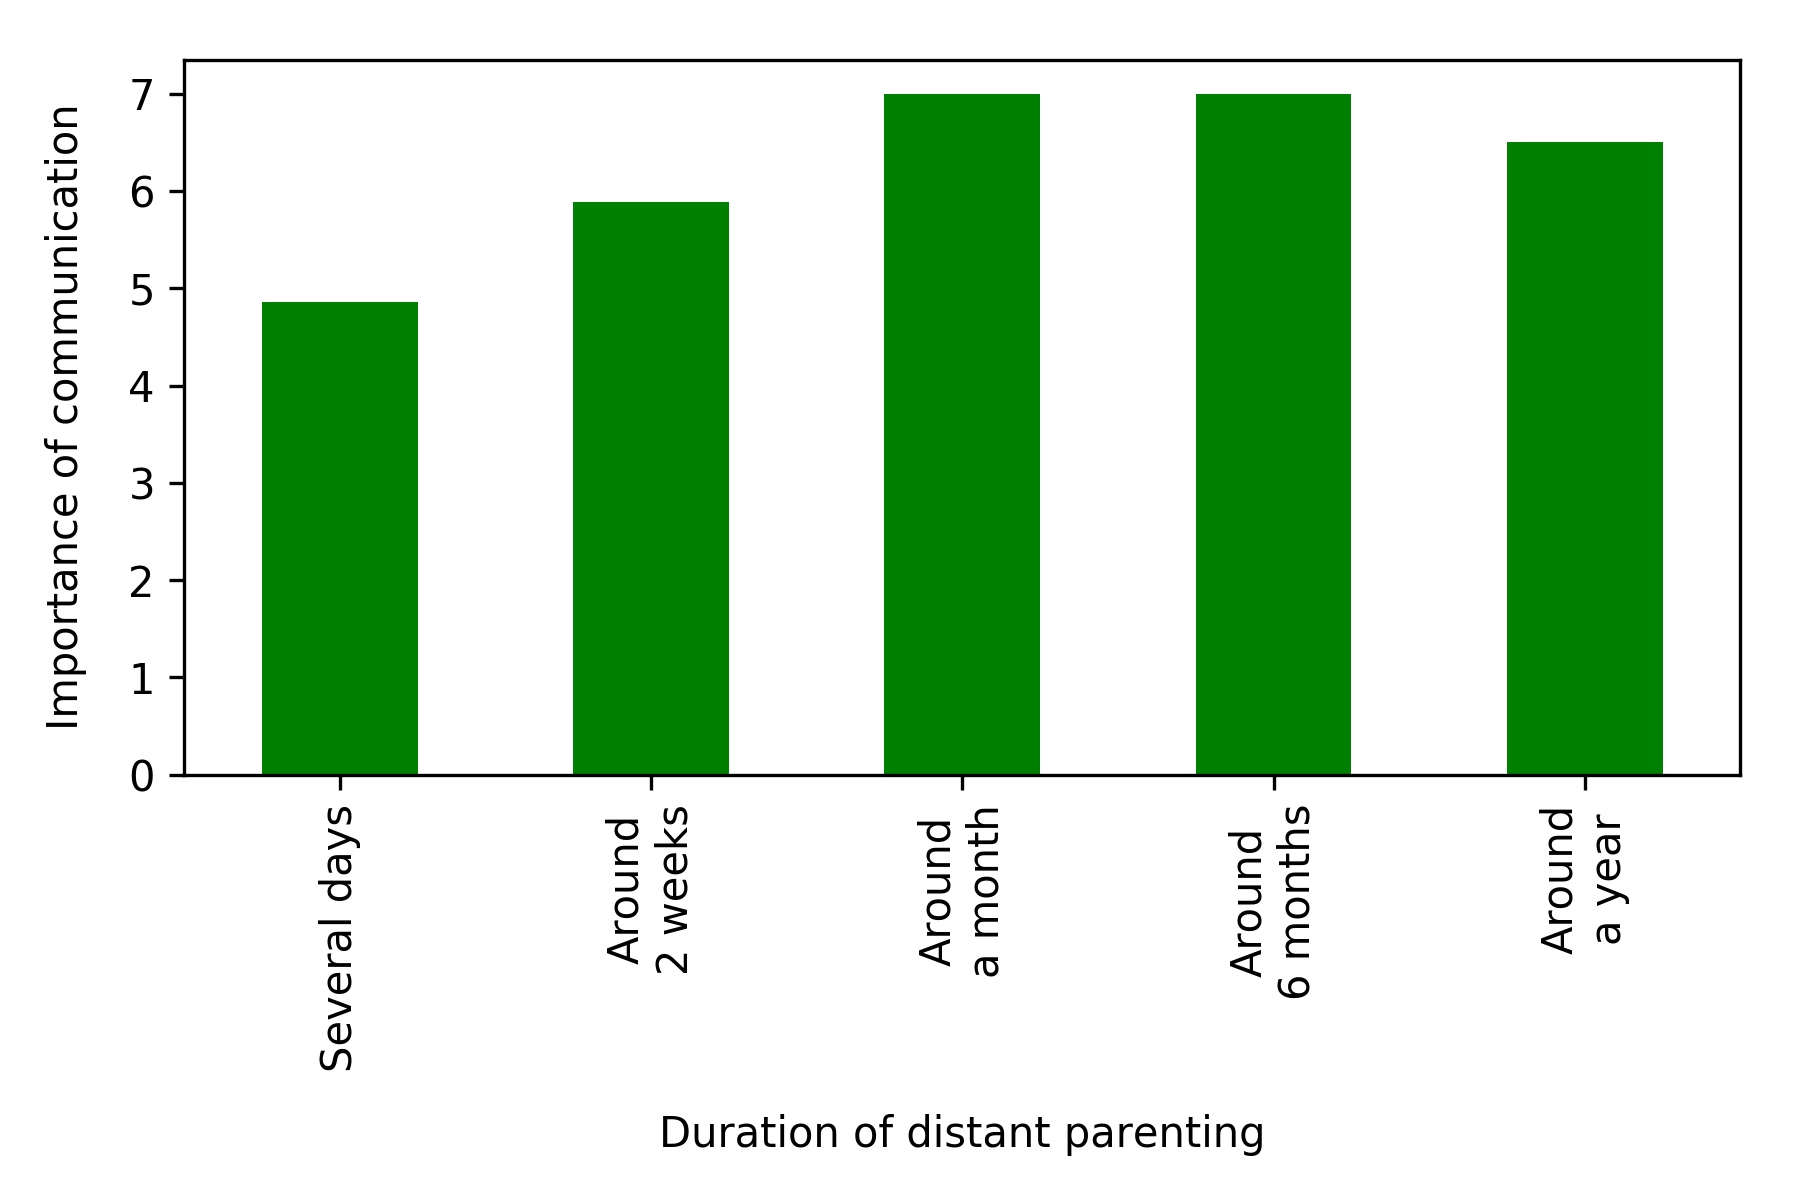
\includegraphics[scale=0.58]{plots/plot_5.png}
    \caption{Importance of communication from the parent point according to duration of distant-parenting experience}
    \label{fig:plot_5}
\end{figure}

\begin{figure}[h!]
    \centering
    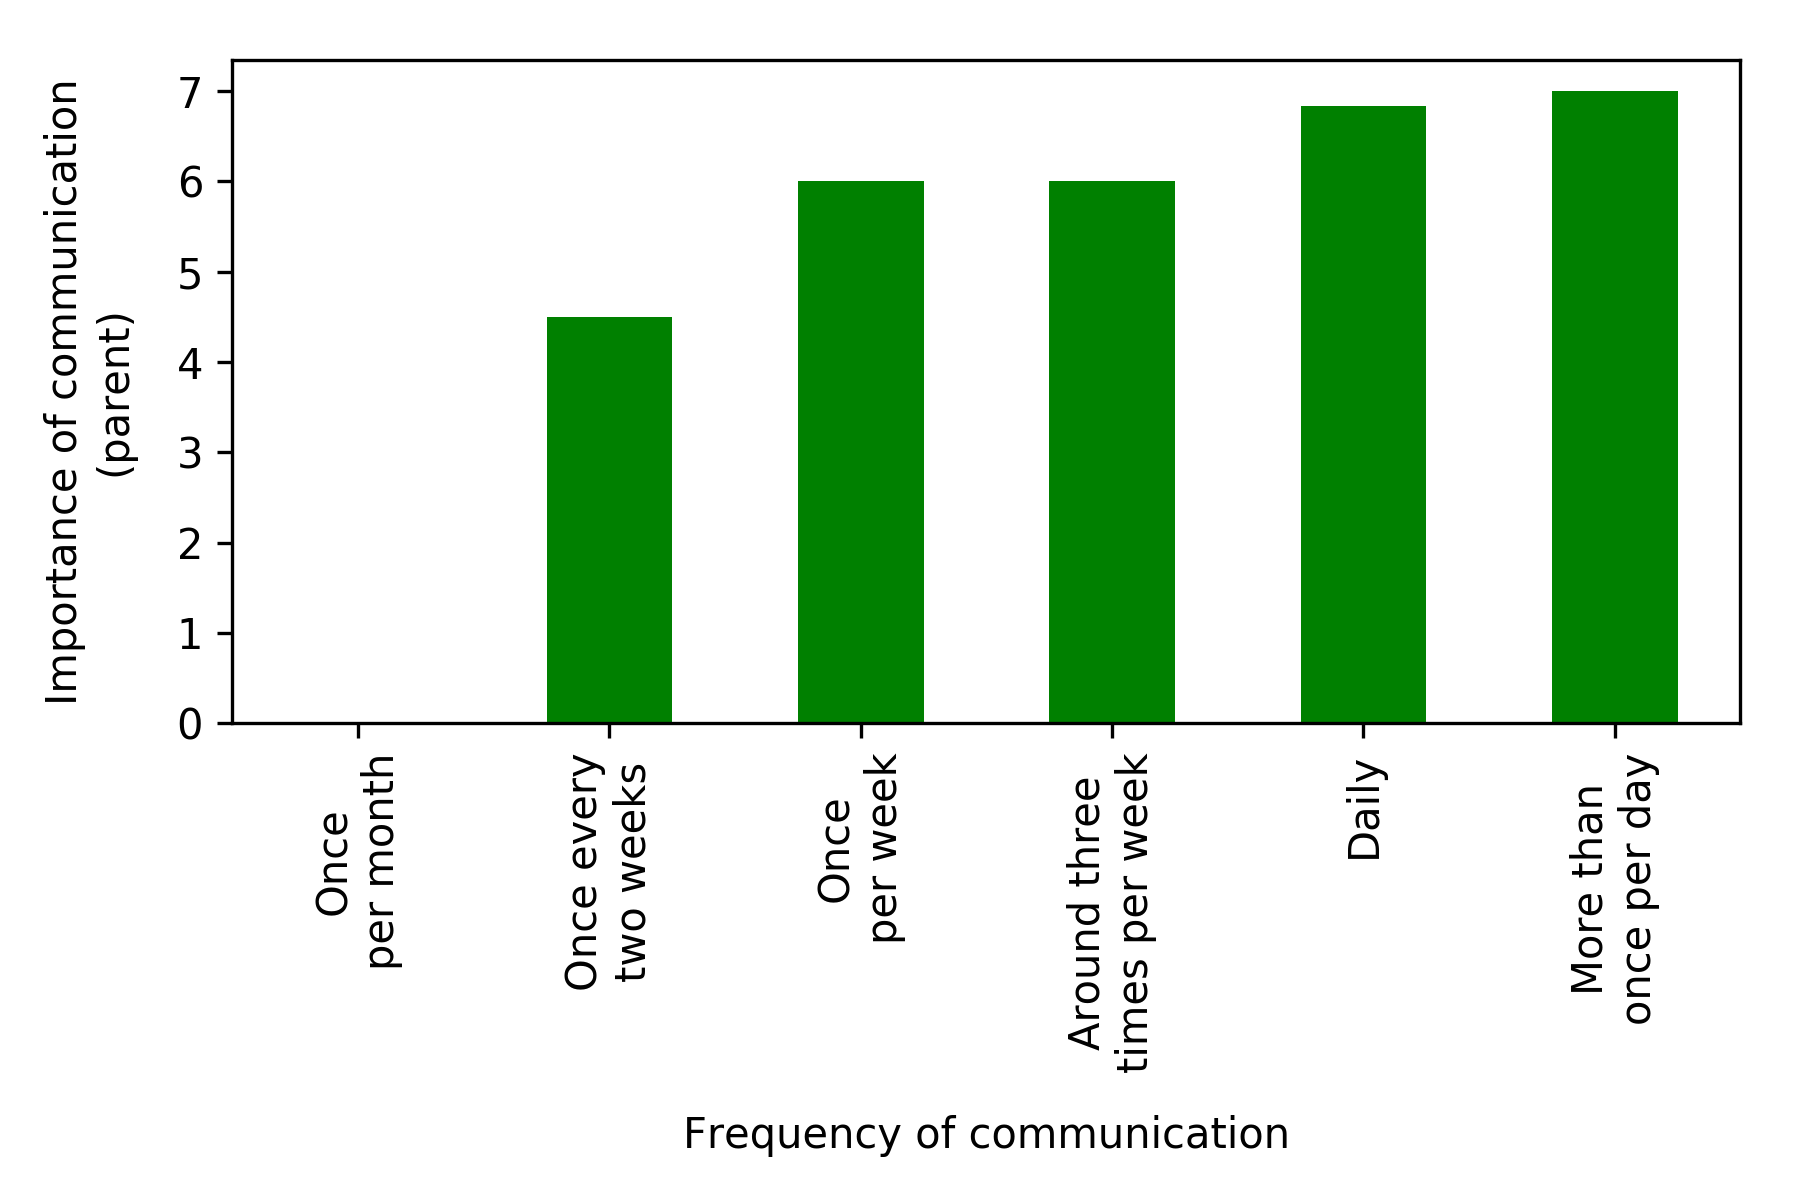
\includegraphics[scale=0.58]{plots/plot_8.png}
    \caption{Importance of communication from the parent point according to frequency of communication during distant-parenting experience}
    \label{fig:plot_8}
\end{figure}


\subsection{Interview protocol}
\label{appendix:interview_protocol}

The following interview protocol has been prepared for the research on “Communication Technologies for Left-Behind Children in Rural China”, in the scope of the “Global perspectives, local realities” SHS course. To continue our research on the Chinese field, by interviewing parents of left behind children, our assumptions could be tested and eventually further analyzed.

\vspace{4pt}
Please, fill in the missing informations as follows before starting the interview session:

Author: Matteo Yann Feo \& Simone Sanso

Session length: 40 minutes 

Participant Name: \hfill \_\_\_\_\_\_\_\_\_\_\_\_\_\_\_\_\_\_\_\_\_\_\_  $\leftarrow$ Fill in

Email: \hfill \_\_\_\_\_\_\_\_\_\_\_\_\_\_\_\_\_\_\_\_\_\_\_\_\_\_\_\_\_\_\_\_ $\leftarrow$ Fill in

Time/Date: \hfill \_\_\_\_\_\_\_\_\_\_\_\_\_\_\_\_\_\_\_\_\_\_\_\_\_\_\_\_ $\leftarrow$ Fill in

Location: \hfill \_\_\_\_\_\_\_\_\_\_\_\_\_\_\_\_\_\_\_\_\_\_\_\_\_\_\_\_\_ $\leftarrow$ Fill in

\vspace{6pt}
\subsubsection{Introduction \& Setup (5 mins)}

The session starts with a short introduction to what this interview is about, the context and the background for which it is being conducted. In the meantime, be sure that everything is setup correctly by double checking the following To-Do list:

\begin{todolist}
    \item Setup the recording tools and check if they work correctly.
    \item Prepare note-taking utilities, such as pen and paper.
    \item Verify the environment, being sure to have a relaxed location for the following 40 mins.
    \item In case a beverage is desired in the meantime, be sure to have it ready and available now.
    \item Be sure that your interviewed person has everything needed.
\end{todolist}

The introduction of the interview could be similar to the following one:

"Good morning and thank you for participating! I am Yann. I am studying at EPFL for a master degree in computer science. My main interest for this interview is to understand whether  a  technology  of  communication embedded in a smart toy could be helpful for parents distant from their children. During the interview, I will be having a conversation with you, asking questions that could help me to achieve my curiosity. In the meantime, my partner, will be assisting me by taking some notes. It is important to always remember that we are not evaluating you or your opinions in any way, there are no possible right and wrong answers that you could give. 
Here is how the session is going to proceed. Firstly, we'll break the ice by asking you a few general questions to know each other. We will record this interview, given your consent. We won't ever share this recording nor use it for anything else but pure support for this interview, so that I can go back and review things later to make sure we got everything right. Your name won't ever be linked to any result, so be relaxed and feel free to share your thoughts with us, without any troubles. Keep in mind that this is completely voluntary, the recording can be stopped whenever you want. Thus, if you don't like this idea, please let me know. 
How does all that sound to you? Do you have any questions at this point?"

\begin{todolist}
    \item Ask the interviewee to sign the written consent for recording purposes.
\end{todolist}

\vspace{2pt}
\subsubsection{Demographics \& Background (5 mins)}

This section will help us to create a background of the interviewee, while allowing him/her to start opening up to our questions. Use this session as a warming-up occasion to break the ice, while catching the first important features. Start to note down details on the interviewee, like gender, age, education level, marital status.

\begin{todolist}
    \item Tell us your name, and a little bit about yourself.
    \item Where do you come from?
    \item What is your occupation? Are you studying or working? In both cases, can you tell us something about it?
    \item Where are you currently living? Do you live with someone, or alone? 
\end{todolist}

\vspace{2pt}
\subsubsection{Main questions (20 mins)}

The following questions can be helpful to interpolate your impressions with the interviewee’s feelings and personal stories. Use them carefully as they might be intimidating for some people. Don’t forget to check for nonverbal behaviors, as they might be critical to have a complete idea of who you are interviewing, especially in this part. Note that the most important questions to be answered are marked with an asterisk (*).

\vspace{2pt}
(*) Pre-interview questions about their children :

\begin{todolist}
    \item How many children do you have?
    \item How old are they?
    \item What gender are they?
    \item Where do you they live?
    \item With who are they staying in your home village? (Lonely, with one of both parents, with grandparents or other relatives)
\end{todolist}

Main interview questions about the interviewed parent :

\begin{todolist}
    \item (*) How often and for how long do you come back home? 
    \item What is the main reason why you live far away from your children?
    \item How do you feel about this situation, not living with your children?
    \item Remember the last time you went back to your home village, how was the contact with your children? Was the meeting with your children as before you left them?
    \item During your childhood, have you ever experienced living far away from one of your parents? If yes, for how long? How did you live the situation? Could you tell us what was the main reason of your parent to out-migrate? How was the contact when meeting again with your parent? Could you communicate together, at that time, while being distant? (Check for non-verbal reactions while interviewee showcase personal experience)
    \item How common is your situation of distant parenting? Do you know any other persons in the same situation as you? How do they live it?
    \item (*) How would you define the importance of living with your children? In your case, is there a trade off between living with your children and having a job position? If yes, imagine that you could live in an ideal world, what would be the best solution? Would you rather work in your home village or be able to bring your children in town?
    \item (*) Do you own electronic devices? If yes, which ones? (Smartphone, computer, more…)
    \item (*) Do your children in your home village own electronic devices? If not, would they have the opportunity to use any? (Neighbourhood, school, etc.)
    \item (*) Do you use electronic devices to contact your children? If yes, how often? In general, are you calling your children when you have time? Or do they also get in touch with you, on their initiative?
    \item (*) From 0 to 7, how would you define the importance of communicating with your children? (0: insignificant, 4: neutral, 7: essential) (Check for non-verbal reactions while interviewee showcase personal experience)
\end{todolist}

\vspace{2pt}
\subsubsection{Interviewee's "show and tell" prototype (8 mins)}

This section is practical and allows us to showcase our project, related to the issue of distant parenting. In the context of CHIC (China Hardware Innovation Camp), a plush toy that encourages social interaction between parents and children, in a distant situation. It is a very resourceful moment, as it could bring additional and authentic feedback on a novel user scenario.

The explanation of the prototype could be similar to the following one:

"We have been working on this prototype. It is a plush toy that encourages social interaction, by having remotely turned on LEDs and sounds from a mobile application. Parents and children can therefore stay longer connected. Letting your children know when you think about them will help you stay 'toygether'\texttrademark."

Showcase the prototype and how it works with the mobile application.

\begin{todolist}
    \item What do you think about the idea?
    \item In your opinion, which are the positive and negative aspects?
    \item If you had the possibility to try this technology, would you be interested?
    \item What would you modify to improve it?
\end{todolist}

\vspace{2pt}
\subsubsection{Closing (2 mins)}

Thank the user at the end for participating to the session. Offer the possibility to ask any kind of question the interviewee might want to address you.  This is his/her time to wear the interviewer's shoes in your regards.

If the interviewee has no additional question, the interview is officially finished. Thank again your interviewee for the time and availability to participate to this session. Underline how useful his/her help has been for the project.
Turn off the recording tools only when you are completely sure that nothing will be added. It is important to not miss anything, so better have some extra recording to cut later.

Take some time to, directly after the end of the interview, write down some impressions you may have about the session. It is important to note down very early impressions about both verbal and physical languages, before they are forgotten. Those are the most authentic resources to get.




\subsection{List of contacts}
\label{appendix:contacts_list}
Below are listed all the contacts that have been reached, to spread as much as possible the survey.

\begin{itemize}
\item AFS programs for adolescents (15-18 years old): \\
Duration: 1 year \\
Kernstrasse 57, CH-8004 Zurich \\
Tel: +41 21 323 19 19 \\
Email: hello@afs.ch \\
https://www.afs.ch/fr/programmes-scolaires/ 

\vspace{4pt}
\item Canada-France exchange (16 years old): \\
Duration : 3 weeks \\
College of Jeanne d'Arc, 15 Rue du Chanoine Brun, 68100 Mulhouse, France \\
Tel: +33 3 89 45 36 31 \\
www.ejda.fr/ 

\vspace{4pt}
\item International exchange programs (14-18 years old): \\
Duration: 1 year \\
Rue Centrale 15, 1003 Lausanne \\
Tel: +41 800 822 811 \\
https://www.efswiss.ch/fr/highschool/ 

\vspace{4pt}
\item National observatory of the Erasmus + impact (1 year or 6 months): \\
Email: observatoire@agence-erasmus.fr \\
http://www.agence-erasmus.fr/page/observatoire/

\vspace{4pt}
\item Journal of international mobility:\\
Email: revue@agence-erasmus.fr \\
https://www.agence-erasmus.fr/page/JIM

\vspace{4pt}
\item Exchange program Brigitte Sauzay (14-17 years old): \\
Duration: 3 months in a host family in Germany and welcome 3 months in the family in France \\
https://www.ofaj.org/contact.html 

\vspace{4pt}
\item Internal exchanges and language stays in Switzerland (14-17 years old): \\
Duration: 1 year \\
College of Delémont, Avenue Station 7, 2800 Delémont \\
Tel: +41 32 421 00 70 \\
Email: info@coldel.org \\
http://www.college-delemont.ch/fr/Aide-aux-eleves/Echanges-et-sejours-linguistiques/Echanges-et-sejours-linguistiques.html \\
Cantonal manager of linguistic exchanges: \\
Patrice KAMBER, Pâquerettes 2, 2822 Courroux \\
- Prof: 032 435 65 92 / Private: 032 422 83 62 

\vspace{4pt}
\item Language Exchange and Mobility - DIP Geneva: \\
Catherine Fernandez Sonino: Head of Exchange \& Mobility DIP of the Cantonal Office for Language Exchange and Mobility \\
Chemin de l'Echo 5a, 1213 Onex \\
Email: catherine.fernandez@etat.ge.ch \\
Tel: +41 22 327 06 43, +41 79 175 56 46 \\
https://edu.ge.ch/site/elem/ 

\vspace{4pt}
\item Service of primary and secondary schools of Lausanne: \\
Place Chauderon 9, 5th floor, PO Box 5032, 1002 Lausanne \\
Tel: +41 21 315 64 11 - Fax: +41 21 315 60 04 \\
Email: seps@lausanne.ch \\
http://www.lausanne.ch/etablissements-scolaires/ 

\vspace{4pt}
\item Summer camp of Neuchatel:\\
Gisèle Nicaty \\
Quartier du Milieu 86, 2127 Les Bayards \\
Tel: +41 79 288 50 41, +41 32 866 17 29\\
Email: giroud.p-a@bluewin.ch\\
http://www.echanges-scolaires.com/index.php/fr/

\vspace{4pt}
\item Summer camp of the Grandes-Roches: \\
1348 le Brassus \\
Tel: +41 21 845 66 90 \\
Email: camps@asime.ch \\
http://www.grandesroches.ch/home 

\vspace{4pt}
\item Association of the Gros-de-Vaud Holiday Camp: \\
Mrs Florence Ethenoz \\
Chemin du Petit Record 60, 1040 Echallens \\
Tel: +41 21 881 10 76 \\
Email: info@colo-gros-de-vaud.ch \\
http://www.colo-gros-de-vaud.ch/clubdesk/www

\vspace{4pt}
\item Summer camp 4Fun: \\
Email: airfred@hotmail.com \\
http://4-fun.ch/ 

\vspace{4pt}
\item Summer camp CPV: \\
Swiss Village Street 14, PO Box 72, 1211 Geneva 8 \\
Tel: +41 22 809 49 79 \\
Email: info@camps.ch \\
http://www.camps.ch/fr/accueil 

\vspace{4pt}
\item Scouts of the Sacred Heart: \\
Jeanne Voruz \& Anne Thiébaud \\
Tel: +41 79 844 92 74 \& +41 79 284 50 38 \\
Email: cg@sacrescout.ch \\
http://www.sacrescout.ch/ 

\vspace{4pt}
\item Village Camps: \\
PO Box 1425, Rue de la Morache 14, 1260 Nyon 1 \\
Tel: +41 22 990 9400 \\
Email: camps@villagecamps.com \\
www.villagecamps.com

\vspace{4pt}
\item Alpadia Language Schools: \\
Grand-Rue 42, PO Box 1206, 1820 Montreux\\
Tel: +41 21 621 88 88\\
Email: info@alpadia.com\\
https://www.alpadia.com/fr/ 

\vspace{4pt}
\item Carol Panchaud Educom sàrl: \\
26 Route of Givrins, CH - 1276 Gingins\\
Tel: +41 22 776 69 15 \\
Email: carolpanchaud@educom.ch \\
http://educom.ch/fr

\vspace{4pt}
\item Caritas-Youth: \\
11, Jean-Violette Street, 1205 Geneva\\
Tel: +41 22 708 04 04\\
Email: info@caritas-jeunesse.ch\\
http://www.caritas-jeunesse.ch/

\vspace{4pt}
\item Holiday Camp St. Gervais: \\
CP 1337, 1211 Geneva 1\\
Tel: +41 78 896 71 84\\
Email: info@colonie-saint-gervais.ch\\
http://www.colonie-saint-gervais.ch/

\vspace{4pt}
\item Summer Camp of Ravoire - Camp Plein Soleil: \\
PO Box 87, CH-1920 Martigny 1\\
Email: info@camp-pleinsoleil.ch

\vspace{4pt}
\item Yverdon-les-Bains youth service and social cohesion: \\
Rue de Neuchâtel 2, 1400 Yverdon-les-Bains\\
Tel: +41 24 423 69 11\\
Email: vacances@yverdon-les-bains.ch\\
http://www.yverdon-les-bains.ch/prestations-deladministration/jeunesse-et-cohesion-sociale/enfanceetfamille/colonies-dete-et-dautomne/

\vspace{4pt}
\item fRilingue GmbH: \\
Stöckackerstrasse 93, 3018 Bern\\
Tel: +41 26 321 34 34 \\
Email: info@frilingue.com

\vspace{4pt}
\item Star Sports: \\
Path of Verger 2, PO Box 101, 1304 Cossonay-Ville\\
Tel: +41 79 356 44 61\\
Email: info@starsports.ch\\
http://www.starsports.ch/

\vspace{4pt}
\item Cap Loisirs Foundation: \\
34, Boulevard de Saint-Georges, 1205 Geneva\\
Tel: +41 22 731 86 00\\
Email: caploisirs@caploisirs.ch\\
http://www.caploisirs.ch/

\vspace{4pt}
\item SCE Holidays \& Events: \\
Rue de Lausanne 58, 1950 Sion\\
Tel: +41 79 693.33.64\\
Email: info@lescamps.ch\\
https://www.lescamps.ch/\\

\end{itemize}



% References of the Report
\thispagestyle{empty}
\vspace{1cm}
\begin{thebibliography}{9}
\addcontentsline{toc}{section}{References}

\bibitem{lab3-report} 
\textit{Lab 3.0 : Camera \& LCD conceptual design}. \\
CS-473 EPFL. Matteo Yann Feo \& Simone Aron Sanso. November 28th, 2017

\bibitem{lcd-controller} 
\textit{ILI9341 - a-Si TFT LCD Single Chip Driver 240RGBx320 Resolution and 262K color}. 
Rev. 1.11. ILI TECHNOLOGY CORP.

\bibitem{lcd-display} 
\textit{LT24 User Manual}. 
Altera. June 2015
 
\bibitem{avalon-interface} 
\textit{Avalon® Interface Specifications}.
MNL-AVABUSREF. Intel. May 2017.
 
\bibitem{fifo} 
\textit{Single- and Dual-Clock FIFO Megafunction}.
Rev. 4.0. Altera. May 2007.

\end{thebibliography}

\end{document}


\documentclass[a4paper,12pt]{article}

%% Layout
\usepackage[utf8]{inputenc}
\usepackage{palatino}
\usepackage[T1]{fontenc}
\usepackage[8pt]{extsizes}

\usepackage{geometry}
\geometry{
    a4paper,
    total={170mm,257mm},
    left=30mm,
    right=30mm,
    top=30mm,
    bottom=30mm,
 } 

%% Useful packages
\usepackage{amsmath}
\usepackage{amssymb}
\usepackage{mathtools}
\usepackage{microtype}

\usepackage[usenames, dvipsnames]{xcolor}
\usepackage{graphicx}
\usepackage{wrapfig}
\usepackage{subfig}
\usepackage{tabularx}
\usepackage{float}
\usepackage{caption}
\usepackage{multirow}
\usepackage{color, colortbl}
\usepackage{enumerate}

\usepackage{hyperref}
\usepackage{url}

\usepackage[english]{babel}
\usepackage{units}

\usepackage{textcomp}
\usepackage{titling}
\usepackage{blindtext}
\usepackage{listings}

\usepackage{braket}
\usepackage{rotating}

%\setlength{\droptitle}{-4em}     % Eliminate the default vertical space
%\addtolength{\droptitle}{-4pt}

\title{
    \centering
	
\includegraphics[width=0.5\textwidth]{images/Logo_EPFL.png}
    \\[1cm]
	\Huge China Hardware Innovation Camp\\[1cm]
    \huge Semester project report\\
    \rule{3.5cm}{0.9pt}\\[0.5cm]
    \huge HUM - 498 \vfill
    \normalsize
}

\author{
    \textbf{Laboratory group:}\\\\
    Chloe Dickson - \texttt{\href{mailto:chloe.dickson@epfl.ch}{simone.sanso@epfl.ch}} \\
    Matteo Yann Feo -    \texttt{\href{mailto:matteo.feo@epfl.ch}{matteo.feo@epfl.ch}} \\
    Simone Aron Sanso - \texttt{\href{mailto:simone.sanso@epfl.ch}{simone.sanso@epfl.ch}} \\\\
}

\date{\vfill \today}

\lstdefinestyle{Python}{
  language=Python,                % choose the language of the code
  numbers=left,                   % where to put the line-numbers
  stepnumber=1,                   % the step between two line-numbers.        
  numbersep=5pt,                  % how far the line-numbers are from the code
  backgroundcolor=\color{white},  % choose the background color. You must add \usepackage{color}
  showspaces=false,               % show spaces adding particular underscores
  showstringspaces=false,         % underline spaces within strings
  showtabs=false,                 % show tabs within strings adding particular underscores
  tabsize=2,                      % sets default tabsize to 2 spaces
  captionpos=b,                   % sets the caption-position to bottom
  breaklines=true,                % sets automatic line breaking
  breakatwhitespace=true,         % sets if automatic breaks should only happen at whitespace
  frame=single, 
  basicstyle=\ttfamily,
  keywordstyle=\color{Green}\bfseries,
  stringstyle=\color{red}\ttfamily,
  commentstyle=\color{OliveGreen}\ttfamily,
  %morecomment=[l][\color{magenta}]{\#}
}


\begin{document}
\maketitle
\thispagestyle{empty}

\newpage
\thispagestyle{empty}
\setcounter{page}{0}

\tableofcontents

\documentclass[a4paper,12pt]{article}

%% Layout
\usepackage[utf8]{inputenc}
\usepackage{palatino}
\usepackage[T1]{fontenc}
\usepackage[8pt]{extsizes}

\usepackage{geometry}
\geometry{
    a4paper,
    total={170mm,257mm},
    left=30mm,
    right=30mm,
    top=30mm,
    bottom=30mm,
 } 

%% Useful packages
\usepackage{amsmath}
\usepackage{amssymb}
\usepackage{mathtools}
\usepackage{microtype}

\usepackage[usenames, dvipsnames]{xcolor}
\usepackage{graphicx}
\usepackage{wrapfig}
\usepackage{subfig}
\usepackage{tabularx}
\usepackage{float}
\usepackage{caption}
\usepackage{multirow}
\usepackage{color, colortbl}
\usepackage{enumerate}

\usepackage{hyperref}
\usepackage{url}

\usepackage[english]{babel}
\usepackage{units}

\usepackage{textcomp}
\usepackage{titling}
\usepackage{blindtext}
\usepackage{listings}

\usepackage{braket}
\usepackage{rotating}

%\setlength{\droptitle}{-4em}     % Eliminate the default vertical space
%\addtolength{\droptitle}{-4pt}

\title{
    \centering
	
\includegraphics[width=0.5\textwidth]{images/Logo_EPFL.png}
    \\[1cm]
	\Huge China Hardware Innovation Camp\\[1cm]
    \huge Semester project report\\
    \rule{3.5cm}{0.9pt}\\[0.5cm]
    \huge HUM - 498 \vfill
    \normalsize
}

\author{
    \textbf{Laboratory group:}\\\\
    Chloe Dickson - \texttt{\href{mailto:chloe.dickson@epfl.ch}{simone.sanso@epfl.ch}} \\
    Matteo Yann Feo -    \texttt{\href{mailto:matteo.feo@epfl.ch}{matteo.feo@epfl.ch}} \\
    Simone Aron Sanso - \texttt{\href{mailto:simone.sanso@epfl.ch}{simone.sanso@epfl.ch}} \\\\
}

\date{\vfill \today}

\lstdefinestyle{Python}{
  language=Python,                % choose the language of the code
  numbers=left,                   % where to put the line-numbers
  stepnumber=1,                   % the step between two line-numbers.        
  numbersep=5pt,                  % how far the line-numbers are from the code
  backgroundcolor=\color{white},  % choose the background color. You must add \usepackage{color}
  showspaces=false,               % show spaces adding particular underscores
  showstringspaces=false,         % underline spaces within strings
  showtabs=false,                 % show tabs within strings adding particular underscores
  tabsize=2,                      % sets default tabsize to 2 spaces
  captionpos=b,                   % sets the caption-position to bottom
  breaklines=true,                % sets automatic line breaking
  breakatwhitespace=true,         % sets if automatic breaks should only happen at whitespace
  frame=single, 
  basicstyle=\ttfamily,
  keywordstyle=\color{Green}\bfseries,
  stringstyle=\color{red}\ttfamily,
  commentstyle=\color{OliveGreen}\ttfamily,
  %morecomment=[l][\color{magenta}]{\#}
}


\begin{document}
\maketitle
\thispagestyle{empty}

\newpage
\thispagestyle{empty}
\setcounter{page}{0}

\tableofcontents

\input{sections/1_introduction/main.tex}

\input{sections/2_structure/main.tex}
    \input{sections/2_structure/subsection_A.tex}
    \input{sections/2_structure/subsection_B.tex}
    \input{sections/2_structure/subsection_C.tex}
    
\input{sections/3_images_tables/main.tex}

\input{sections/4_code/main.tex}

\input{sections/5_conclusion/main.tex}

\input{appendix.tex}

\input{bibliography.tex}

\end{document}


\documentclass[a4paper,12pt]{article}

%% Layout
\usepackage[utf8]{inputenc}
\usepackage{palatino}
\usepackage[T1]{fontenc}
\usepackage[8pt]{extsizes}

\usepackage{geometry}
\geometry{
    a4paper,
    total={170mm,257mm},
    left=30mm,
    right=30mm,
    top=30mm,
    bottom=30mm,
 } 

%% Useful packages
\usepackage{amsmath}
\usepackage{amssymb}
\usepackage{mathtools}
\usepackage{microtype}

\usepackage[usenames, dvipsnames]{xcolor}
\usepackage{graphicx}
\usepackage{wrapfig}
\usepackage{subfig}
\usepackage{tabularx}
\usepackage{float}
\usepackage{caption}
\usepackage{multirow}
\usepackage{color, colortbl}
\usepackage{enumerate}

\usepackage{hyperref}
\usepackage{url}

\usepackage[english]{babel}
\usepackage{units}

\usepackage{textcomp}
\usepackage{titling}
\usepackage{blindtext}
\usepackage{listings}

\usepackage{braket}
\usepackage{rotating}

%\setlength{\droptitle}{-4em}     % Eliminate the default vertical space
%\addtolength{\droptitle}{-4pt}

\title{
    \centering
	
\includegraphics[width=0.5\textwidth]{images/Logo_EPFL.png}
    \\[1cm]
	\Huge China Hardware Innovation Camp\\[1cm]
    \huge Semester project report\\
    \rule{3.5cm}{0.9pt}\\[0.5cm]
    \huge HUM - 498 \vfill
    \normalsize
}

\author{
    \textbf{Laboratory group:}\\\\
    Chloe Dickson - \texttt{\href{mailto:chloe.dickson@epfl.ch}{simone.sanso@epfl.ch}} \\
    Matteo Yann Feo -    \texttt{\href{mailto:matteo.feo@epfl.ch}{matteo.feo@epfl.ch}} \\
    Simone Aron Sanso - \texttt{\href{mailto:simone.sanso@epfl.ch}{simone.sanso@epfl.ch}} \\\\
}

\date{\vfill \today}

\lstdefinestyle{Python}{
  language=Python,                % choose the language of the code
  numbers=left,                   % where to put the line-numbers
  stepnumber=1,                   % the step between two line-numbers.        
  numbersep=5pt,                  % how far the line-numbers are from the code
  backgroundcolor=\color{white},  % choose the background color. You must add \usepackage{color}
  showspaces=false,               % show spaces adding particular underscores
  showstringspaces=false,         % underline spaces within strings
  showtabs=false,                 % show tabs within strings adding particular underscores
  tabsize=2,                      % sets default tabsize to 2 spaces
  captionpos=b,                   % sets the caption-position to bottom
  breaklines=true,                % sets automatic line breaking
  breakatwhitespace=true,         % sets if automatic breaks should only happen at whitespace
  frame=single, 
  basicstyle=\ttfamily,
  keywordstyle=\color{Green}\bfseries,
  stringstyle=\color{red}\ttfamily,
  commentstyle=\color{OliveGreen}\ttfamily,
  %morecomment=[l][\color{magenta}]{\#}
}


\begin{document}
\maketitle
\thispagestyle{empty}

\newpage
\thispagestyle{empty}
\setcounter{page}{0}

\tableofcontents

\input{sections/1_introduction/main.tex}

\input{sections/2_structure/main.tex}
    \input{sections/2_structure/subsection_A.tex}
    \input{sections/2_structure/subsection_B.tex}
    \input{sections/2_structure/subsection_C.tex}
    
\input{sections/3_images_tables/main.tex}

\input{sections/4_code/main.tex}

\input{sections/5_conclusion/main.tex}

\input{appendix.tex}

\input{bibliography.tex}

\end{document}

    %\newpage
\subsection{Subsection A}
\label{subsec:A} 

This is the first subsection. I am saved into a file \textit{subsection\_A.tex} in the same folder as my main file. Pay attention to the format in the label tag in order to reference to the subsection elsewhere. The subsection is called in the main file of the whole document !

\medskip Nunc pulvinar, risus sed gravida pretium, eros tellus vehicula turpis, eget bibendum nisi dolor sed erat. Pellentesque sit amet orci sed ligula dictum cursus. Morbi gravida ligula sapien, non tristique orci semper id. Ut sollicitudin est ut nisi eleifend sollicitudin. Vivamus blandit congue risus id porttitor. Donec sed blandit mauris. Integer est leo, dapibus sed felis et, vulputate sagittis enim. Quisque eget purus vitae metus placerat rhoncus. Nulla eget lacus nec felis tincidunt suscipit ac eget tellus. Ut at augue fermentum, mattis justo sed, consectetur quam. Donec blandit euismod nisi ac auctor.
    %\newpage
\subsection{Subsection B}
\label{subsec:B} 

This is the second subsection. I am also saved into a file \textit{subsection\_B.tex} in the same folder as my main file. Pay attention to the format in the label tag in order to reference to the subsection elsewhere. The subsection is called in the main file of the whole document !

\medskip Nunc pulvinar, risus sed gravida pretium, eros tellus vehicula turpis, eget bibendum nisi dolor sed erat. Pellentesque sit amet orci sed ligula dictum cursus. Morbi gravida ligula sapien, non tristique orci semper id. Ut sollicitudin est ut nisi eleifend sollicitudin. Vivamus blandit congue risus id porttitor. Donec sed blandit mauris. Integer est leo, dapibus sed felis et, vulputate sagittis enim. Quisque eget purus vitae metus placerat rhoncus. Nulla eget lacus nec felis tincidunt suscipit ac eget tellus. Ut at augue fermentum, mattis justo sed, consectetur quam. Donec blandit euismod nisi ac auctor.
    %\newpage
\subsection{Subsection C}
\label{subsec:C} 

Okay, you got it by now ;-)
    
\documentclass[a4paper,12pt]{article}

%% Layout
\usepackage[utf8]{inputenc}
\usepackage{palatino}
\usepackage[T1]{fontenc}
\usepackage[8pt]{extsizes}

\usepackage{geometry}
\geometry{
    a4paper,
    total={170mm,257mm},
    left=30mm,
    right=30mm,
    top=30mm,
    bottom=30mm,
 } 

%% Useful packages
\usepackage{amsmath}
\usepackage{amssymb}
\usepackage{mathtools}
\usepackage{microtype}

\usepackage[usenames, dvipsnames]{xcolor}
\usepackage{graphicx}
\usepackage{wrapfig}
\usepackage{subfig}
\usepackage{tabularx}
\usepackage{float}
\usepackage{caption}
\usepackage{multirow}
\usepackage{color, colortbl}
\usepackage{enumerate}

\usepackage{hyperref}
\usepackage{url}

\usepackage[english]{babel}
\usepackage{units}

\usepackage{textcomp}
\usepackage{titling}
\usepackage{blindtext}
\usepackage{listings}

\usepackage{braket}
\usepackage{rotating}

%\setlength{\droptitle}{-4em}     % Eliminate the default vertical space
%\addtolength{\droptitle}{-4pt}

\title{
    \centering
	
\includegraphics[width=0.5\textwidth]{images/Logo_EPFL.png}
    \\[1cm]
	\Huge China Hardware Innovation Camp\\[1cm]
    \huge Semester project report\\
    \rule{3.5cm}{0.9pt}\\[0.5cm]
    \huge HUM - 498 \vfill
    \normalsize
}

\author{
    \textbf{Laboratory group:}\\\\
    Chloe Dickson - \texttt{\href{mailto:chloe.dickson@epfl.ch}{simone.sanso@epfl.ch}} \\
    Matteo Yann Feo -    \texttt{\href{mailto:matteo.feo@epfl.ch}{matteo.feo@epfl.ch}} \\
    Simone Aron Sanso - \texttt{\href{mailto:simone.sanso@epfl.ch}{simone.sanso@epfl.ch}} \\\\
}

\date{\vfill \today}

\lstdefinestyle{Python}{
  language=Python,                % choose the language of the code
  numbers=left,                   % where to put the line-numbers
  stepnumber=1,                   % the step between two line-numbers.        
  numbersep=5pt,                  % how far the line-numbers are from the code
  backgroundcolor=\color{white},  % choose the background color. You must add \usepackage{color}
  showspaces=false,               % show spaces adding particular underscores
  showstringspaces=false,         % underline spaces within strings
  showtabs=false,                 % show tabs within strings adding particular underscores
  tabsize=2,                      % sets default tabsize to 2 spaces
  captionpos=b,                   % sets the caption-position to bottom
  breaklines=true,                % sets automatic line breaking
  breakatwhitespace=true,         % sets if automatic breaks should only happen at whitespace
  frame=single, 
  basicstyle=\ttfamily,
  keywordstyle=\color{Green}\bfseries,
  stringstyle=\color{red}\ttfamily,
  commentstyle=\color{OliveGreen}\ttfamily,
  %morecomment=[l][\color{magenta}]{\#}
}


\begin{document}
\maketitle
\thispagestyle{empty}

\newpage
\thispagestyle{empty}
\setcounter{page}{0}

\tableofcontents

\input{sections/1_introduction/main.tex}

\input{sections/2_structure/main.tex}
    \input{sections/2_structure/subsection_A.tex}
    \input{sections/2_structure/subsection_B.tex}
    \input{sections/2_structure/subsection_C.tex}
    
\input{sections/3_images_tables/main.tex}

\input{sections/4_code/main.tex}

\input{sections/5_conclusion/main.tex}

\input{appendix.tex}

\input{bibliography.tex}

\end{document}


\documentclass[a4paper,12pt]{article}

%% Layout
\usepackage[utf8]{inputenc}
\usepackage{palatino}
\usepackage[T1]{fontenc}
\usepackage[8pt]{extsizes}

\usepackage{geometry}
\geometry{
    a4paper,
    total={170mm,257mm},
    left=30mm,
    right=30mm,
    top=30mm,
    bottom=30mm,
 } 

%% Useful packages
\usepackage{amsmath}
\usepackage{amssymb}
\usepackage{mathtools}
\usepackage{microtype}

\usepackage[usenames, dvipsnames]{xcolor}
\usepackage{graphicx}
\usepackage{wrapfig}
\usepackage{subfig}
\usepackage{tabularx}
\usepackage{float}
\usepackage{caption}
\usepackage{multirow}
\usepackage{color, colortbl}
\usepackage{enumerate}

\usepackage{hyperref}
\usepackage{url}

\usepackage[english]{babel}
\usepackage{units}

\usepackage{textcomp}
\usepackage{titling}
\usepackage{blindtext}
\usepackage{listings}

\usepackage{braket}
\usepackage{rotating}

%\setlength{\droptitle}{-4em}     % Eliminate the default vertical space
%\addtolength{\droptitle}{-4pt}

\title{
    \centering
	
\includegraphics[width=0.5\textwidth]{images/Logo_EPFL.png}
    \\[1cm]
	\Huge China Hardware Innovation Camp\\[1cm]
    \huge Semester project report\\
    \rule{3.5cm}{0.9pt}\\[0.5cm]
    \huge HUM - 498 \vfill
    \normalsize
}

\author{
    \textbf{Laboratory group:}\\\\
    Chloe Dickson - \texttt{\href{mailto:chloe.dickson@epfl.ch}{simone.sanso@epfl.ch}} \\
    Matteo Yann Feo -    \texttt{\href{mailto:matteo.feo@epfl.ch}{matteo.feo@epfl.ch}} \\
    Simone Aron Sanso - \texttt{\href{mailto:simone.sanso@epfl.ch}{simone.sanso@epfl.ch}} \\\\
}

\date{\vfill \today}

\lstdefinestyle{Python}{
  language=Python,                % choose the language of the code
  numbers=left,                   % where to put the line-numbers
  stepnumber=1,                   % the step between two line-numbers.        
  numbersep=5pt,                  % how far the line-numbers are from the code
  backgroundcolor=\color{white},  % choose the background color. You must add \usepackage{color}
  showspaces=false,               % show spaces adding particular underscores
  showstringspaces=false,         % underline spaces within strings
  showtabs=false,                 % show tabs within strings adding particular underscores
  tabsize=2,                      % sets default tabsize to 2 spaces
  captionpos=b,                   % sets the caption-position to bottom
  breaklines=true,                % sets automatic line breaking
  breakatwhitespace=true,         % sets if automatic breaks should only happen at whitespace
  frame=single, 
  basicstyle=\ttfamily,
  keywordstyle=\color{Green}\bfseries,
  stringstyle=\color{red}\ttfamily,
  commentstyle=\color{OliveGreen}\ttfamily,
  %morecomment=[l][\color{magenta}]{\#}
}


\begin{document}
\maketitle
\thispagestyle{empty}

\newpage
\thispagestyle{empty}
\setcounter{page}{0}

\tableofcontents

\input{sections/1_introduction/main.tex}

\input{sections/2_structure/main.tex}
    \input{sections/2_structure/subsection_A.tex}
    \input{sections/2_structure/subsection_B.tex}
    \input{sections/2_structure/subsection_C.tex}
    
\input{sections/3_images_tables/main.tex}

\input{sections/4_code/main.tex}

\input{sections/5_conclusion/main.tex}

\input{appendix.tex}

\input{bibliography.tex}

\end{document}


\documentclass[a4paper,12pt]{article}

%% Layout
\usepackage[utf8]{inputenc}
\usepackage{palatino}
\usepackage[T1]{fontenc}
\usepackage[8pt]{extsizes}

\usepackage{geometry}
\geometry{
    a4paper,
    total={170mm,257mm},
    left=30mm,
    right=30mm,
    top=30mm,
    bottom=30mm,
 } 

%% Useful packages
\usepackage{amsmath}
\usepackage{amssymb}
\usepackage{mathtools}
\usepackage{microtype}

\usepackage[usenames, dvipsnames]{xcolor}
\usepackage{graphicx}
\usepackage{wrapfig}
\usepackage{subfig}
\usepackage{tabularx}
\usepackage{float}
\usepackage{caption}
\usepackage{multirow}
\usepackage{color, colortbl}
\usepackage{enumerate}

\usepackage{hyperref}
\usepackage{url}

\usepackage[english]{babel}
\usepackage{units}

\usepackage{textcomp}
\usepackage{titling}
\usepackage{blindtext}
\usepackage{listings}

\usepackage{braket}
\usepackage{rotating}

%\setlength{\droptitle}{-4em}     % Eliminate the default vertical space
%\addtolength{\droptitle}{-4pt}

\title{
    \centering
	
\includegraphics[width=0.5\textwidth]{images/Logo_EPFL.png}
    \\[1cm]
	\Huge China Hardware Innovation Camp\\[1cm]
    \huge Semester project report\\
    \rule{3.5cm}{0.9pt}\\[0.5cm]
    \huge HUM - 498 \vfill
    \normalsize
}

\author{
    \textbf{Laboratory group:}\\\\
    Chloe Dickson - \texttt{\href{mailto:chloe.dickson@epfl.ch}{simone.sanso@epfl.ch}} \\
    Matteo Yann Feo -    \texttt{\href{mailto:matteo.feo@epfl.ch}{matteo.feo@epfl.ch}} \\
    Simone Aron Sanso - \texttt{\href{mailto:simone.sanso@epfl.ch}{simone.sanso@epfl.ch}} \\\\
}

\date{\vfill \today}

\lstdefinestyle{Python}{
  language=Python,                % choose the language of the code
  numbers=left,                   % where to put the line-numbers
  stepnumber=1,                   % the step between two line-numbers.        
  numbersep=5pt,                  % how far the line-numbers are from the code
  backgroundcolor=\color{white},  % choose the background color. You must add \usepackage{color}
  showspaces=false,               % show spaces adding particular underscores
  showstringspaces=false,         % underline spaces within strings
  showtabs=false,                 % show tabs within strings adding particular underscores
  tabsize=2,                      % sets default tabsize to 2 spaces
  captionpos=b,                   % sets the caption-position to bottom
  breaklines=true,                % sets automatic line breaking
  breakatwhitespace=true,         % sets if automatic breaks should only happen at whitespace
  frame=single, 
  basicstyle=\ttfamily,
  keywordstyle=\color{Green}\bfseries,
  stringstyle=\color{red}\ttfamily,
  commentstyle=\color{OliveGreen}\ttfamily,
  %morecomment=[l][\color{magenta}]{\#}
}


\begin{document}
\maketitle
\thispagestyle{empty}

\newpage
\thispagestyle{empty}
\setcounter{page}{0}

\tableofcontents

\input{sections/1_introduction/main.tex}

\input{sections/2_structure/main.tex}
    \input{sections/2_structure/subsection_A.tex}
    \input{sections/2_structure/subsection_B.tex}
    \input{sections/2_structure/subsection_C.tex}
    
\input{sections/3_images_tables/main.tex}

\input{sections/4_code/main.tex}

\input{sections/5_conclusion/main.tex}

\input{appendix.tex}

\input{bibliography.tex}

\end{document}


% Appendix of the Report
\appendix

In the following appendix are presented the questions of the survey (... a list of figures and tables) to the reader.

\subsection{Questions of the survey}
\label{appendix:survey_questions}
In this section is shown how the participants were questioned towards the survey. Only the questions in English will be shown here, skipping the French translations.

\medskip \textit{Form about communication technologies :} \\
Realizing a research project about social sciences within EPFL University (Lausanne), we would like to understand the importance of communication between parents and children, when they are at a distance during a continuous period of time.

\vspace{4pt}
1. In what language would like to answer this form?

2. To contextualize, we seek either :

- parents of a child having spent a period of time away from the household,

- children, teenagers and young adults having spent a period of time away from their family.

After having read the description above, do you qualify yourself as a parent or a child?

\vspace{4pt}
\noindent - If "parent" was selected question 2: 

3.a. Are you the mother or the father?

4.a. Have you already been separated from your child for at least 3 days? (Exchange semester abroad, holidays, summer camp, boy-scout, etc.)

5.a. If there were more than one experience of distance parenting, please consider the earliest one of them through the rest of the form (when you were the youngest). What is the reason why your child was distant from you? 

6.a. For how long have you been distant from your child?

7.a. How old was your child at that time?

8.a. What is your child's gender?

9.a. How often did you use a communication technology with your distant child? (Text messages, phone calls, video chat, etc.)

10.a. What kind of information did you seek from communicating with your distant child?

11.a. How would you define the importance of being able to communicate with your distant child?

\vspace{4pt}
\noindent - If "child" was selected question 2: 

3.b. Have you already been separated from your family for at least 3 days? (Exchange semester abroad, holidays, summer camp, boy-scout, etc.)

3.b. If there were more than one experience of separation from your family, please consider the earliest one of them through the rest of the form (when you were the youngest). What is the reason why you were distant from your family? 

4.b. For how long have you been away?

5.b. How old were you at that time?

6.b. What is your gender?

7.b. How often did you use a communication technology with your family? (Text messages, phone calls, video chat, etc.)

8.b. What kind of information did you seek from communicating with your family?

9.b. How would you define the importance of being able to communicate with your family?


\subsection{Additional plots of the results}
\label{appendix:additional-plots}

The following plots have been computed for the analysis of the data collected via the survey on distant-parenting. This appendix contains a set of plots that didn't need particular attention during the discussion, but can still be source of investigation.

\begin{figure}[h!]
    \centering
    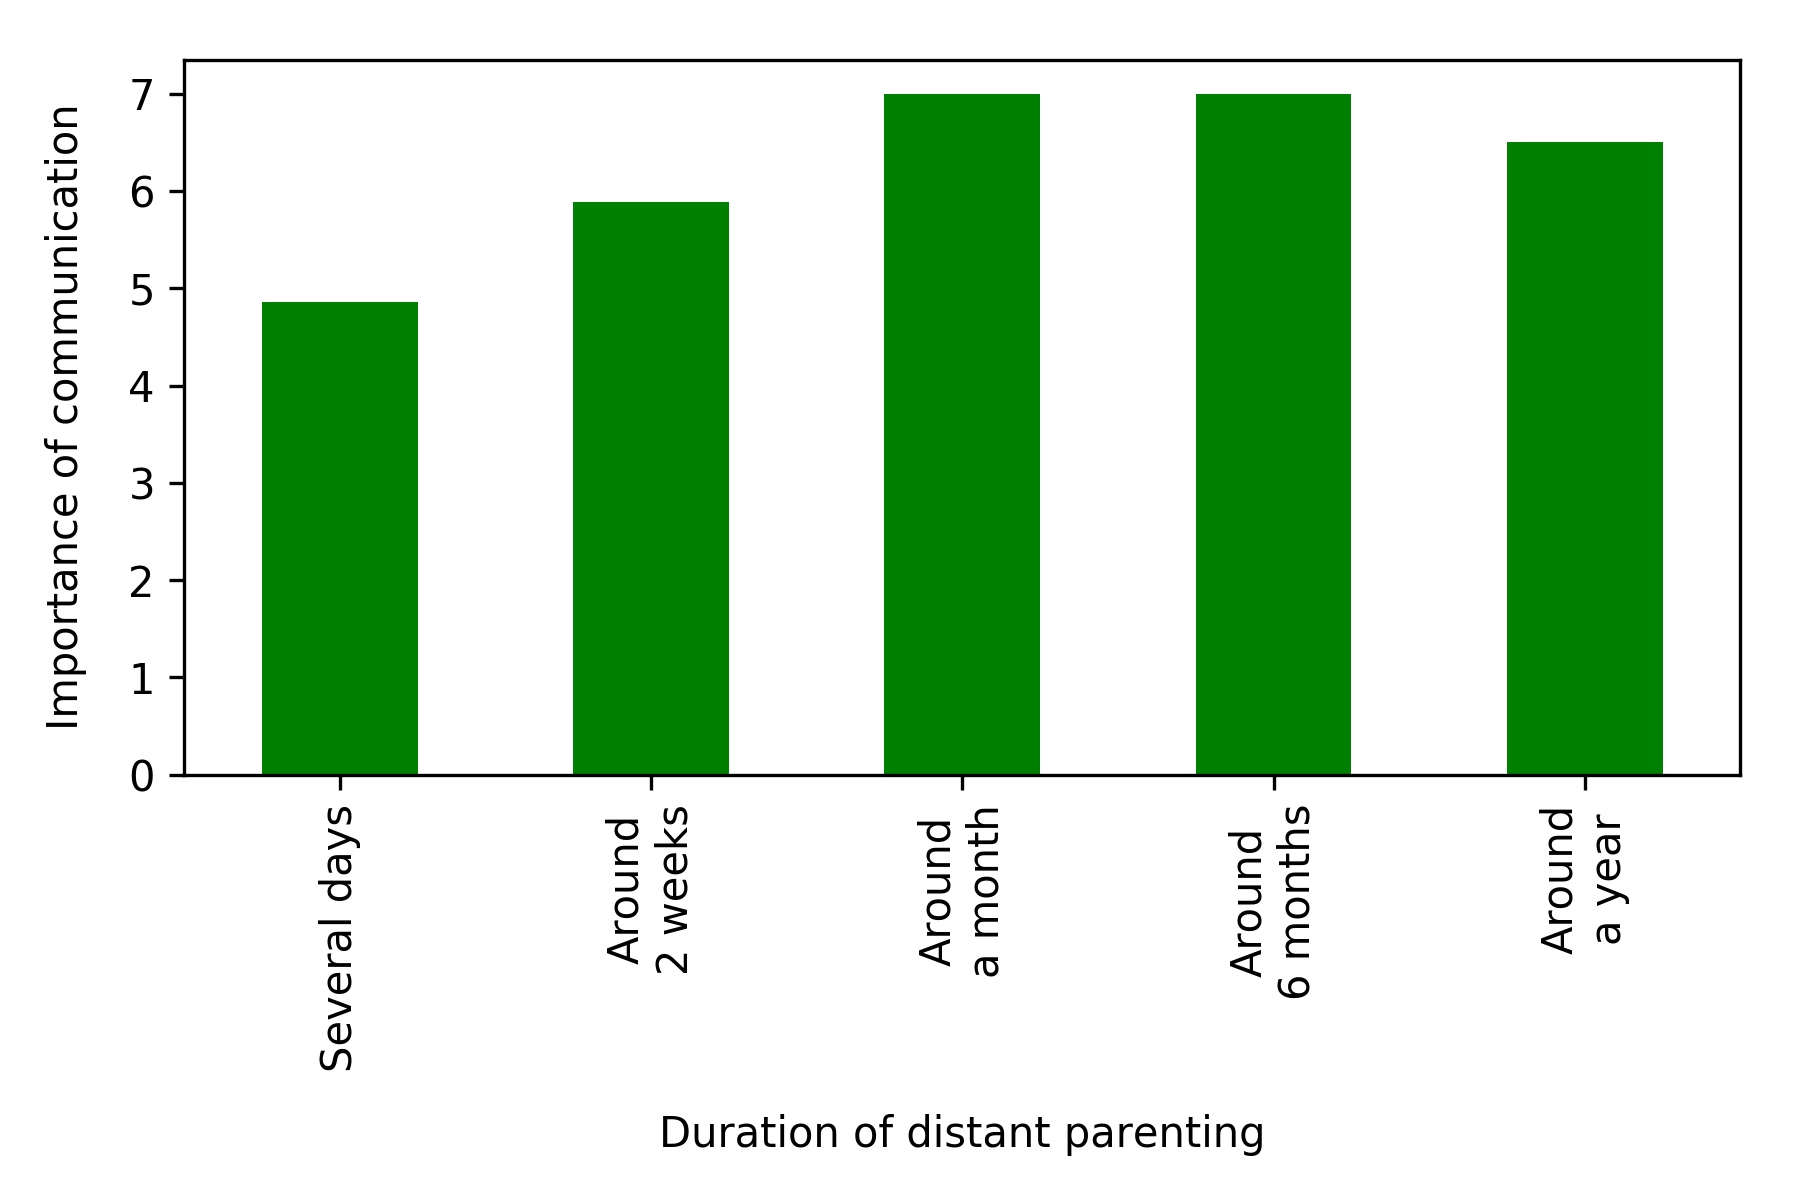
\includegraphics[scale=0.58]{plots/plot_5.png}
    \caption{Importance of communication from the parent point according to duration of distant-parenting experience}
    \label{fig:plot_5}
\end{figure}

\begin{figure}[h!]
    \centering
    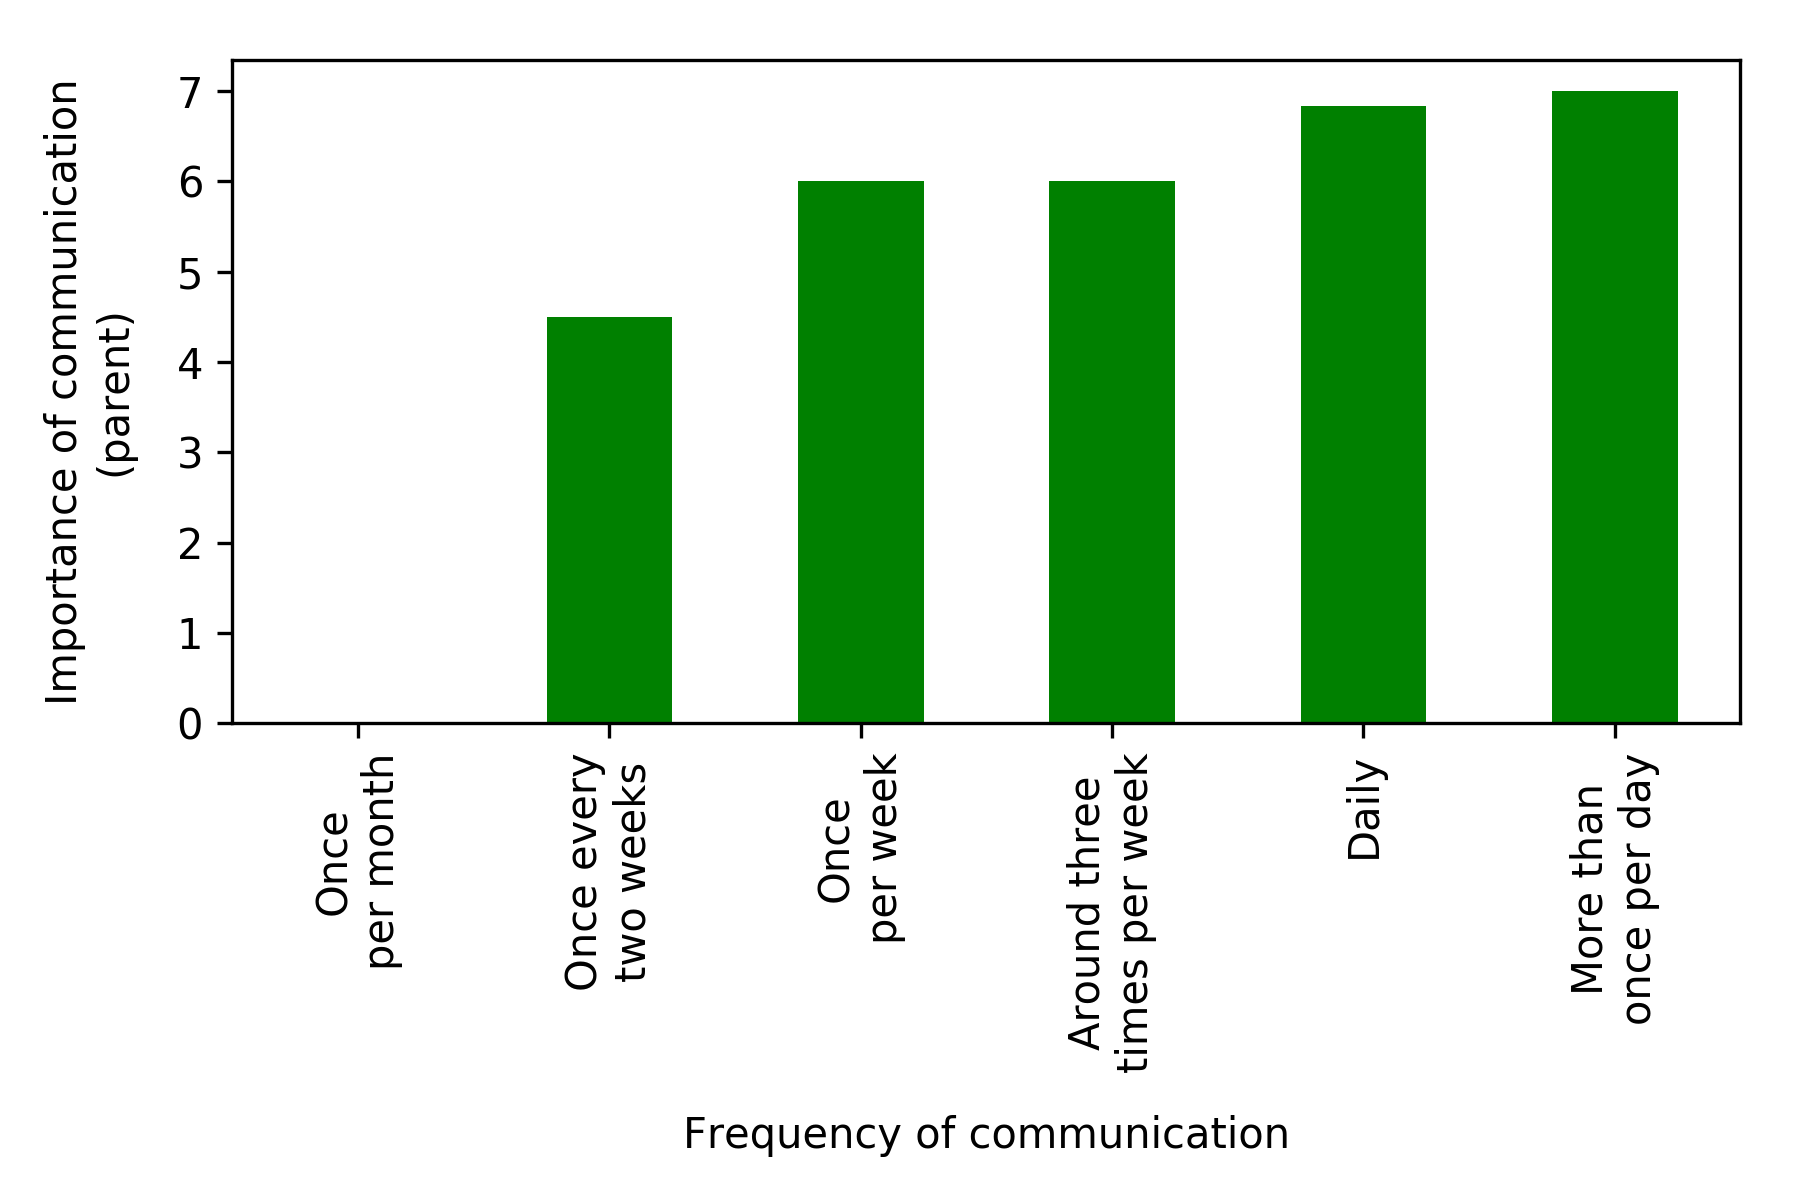
\includegraphics[scale=0.58]{plots/plot_8.png}
    \caption{Importance of communication from the parent point according to frequency of communication during distant-parenting experience}
    \label{fig:plot_8}
\end{figure}


\subsection{Interview protocol}
\label{appendix:interview_protocol}

The following interview protocol has been prepared for the research on “Communication Technologies for Left-Behind Children in Rural China”, in the scope of the “Global perspectives, local realities” SHS course. To continue our research on the Chinese field, by interviewing parents of left behind children, our assumptions could be tested and eventually further analyzed.

\vspace{4pt}
Please, fill in the missing informations as follows before starting the interview session:

Author: Matteo Yann Feo \& Simone Sanso

Session length: 40 minutes 

Participant Name: \hfill \_\_\_\_\_\_\_\_\_\_\_\_\_\_\_\_\_\_\_\_\_\_\_  $\leftarrow$ Fill in

Email: \hfill \_\_\_\_\_\_\_\_\_\_\_\_\_\_\_\_\_\_\_\_\_\_\_\_\_\_\_\_\_\_\_\_ $\leftarrow$ Fill in

Time/Date: \hfill \_\_\_\_\_\_\_\_\_\_\_\_\_\_\_\_\_\_\_\_\_\_\_\_\_\_\_\_ $\leftarrow$ Fill in

Location: \hfill \_\_\_\_\_\_\_\_\_\_\_\_\_\_\_\_\_\_\_\_\_\_\_\_\_\_\_\_\_ $\leftarrow$ Fill in

\vspace{6pt}
\subsubsection{Introduction \& Setup (5 mins)}

The session starts with a short introduction to what this interview is about, the context and the background for which it is being conducted. In the meantime, be sure that everything is setup correctly by double checking the following To-Do list:

\begin{todolist}
    \item Setup the recording tools and check if they work correctly.
    \item Prepare note-taking utilities, such as pen and paper.
    \item Verify the environment, being sure to have a relaxed location for the following 40 mins.
    \item In case a beverage is desired in the meantime, be sure to have it ready and available now.
    \item Be sure that your interviewed person has everything needed.
\end{todolist}

The introduction of the interview could be similar to the following one:

"Good morning and thank you for participating! I am Yann. I am studying at EPFL for a master degree in computer science. My main interest for this interview is to understand whether  a  technology  of  communication embedded in a smart toy could be helpful for parents distant from their children. During the interview, I will be having a conversation with you, asking questions that could help me to achieve my curiosity. In the meantime, my partner, will be assisting me by taking some notes. It is important to always remember that we are not evaluating you or your opinions in any way, there are no possible right and wrong answers that you could give. 
Here is how the session is going to proceed. Firstly, we'll break the ice by asking you a few general questions to know each other. We will record this interview, given your consent. We won't ever share this recording nor use it for anything else but pure support for this interview, so that I can go back and review things later to make sure we got everything right. Your name won't ever be linked to any result, so be relaxed and feel free to share your thoughts with us, without any troubles. Keep in mind that this is completely voluntary, the recording can be stopped whenever you want. Thus, if you don't like this idea, please let me know. 
How does all that sound to you? Do you have any questions at this point?"

\begin{todolist}
    \item Ask the interviewee to sign the written consent for recording purposes.
\end{todolist}

\vspace{2pt}
\subsubsection{Demographics \& Background (5 mins)}

This section will help us to create a background of the interviewee, while allowing him/her to start opening up to our questions. Use this session as a warming-up occasion to break the ice, while catching the first important features. Start to note down details on the interviewee, like gender, age, education level, marital status.

\begin{todolist}
    \item Tell us your name, and a little bit about yourself.
    \item Where do you come from?
    \item What is your occupation? Are you studying or working? In both cases, can you tell us something about it?
    \item Where are you currently living? Do you live with someone, or alone? 
\end{todolist}

\vspace{2pt}
\subsubsection{Main questions (20 mins)}

The following questions can be helpful to interpolate your impressions with the interviewee’s feelings and personal stories. Use them carefully as they might be intimidating for some people. Don’t forget to check for nonverbal behaviors, as they might be critical to have a complete idea of who you are interviewing, especially in this part. Note that the most important questions to be answered are marked with an asterisk (*).

\vspace{2pt}
(*) Pre-interview questions about their children :

\begin{todolist}
    \item How many children do you have?
    \item How old are they?
    \item What gender are they?
    \item Where do you they live?
    \item With who are they staying in your home village? (Lonely, with one of both parents, with grandparents or other relatives)
\end{todolist}

Main interview questions about the interviewed parent :

\begin{todolist}
    \item (*) How often and for how long do you come back home? 
    \item What is the main reason why you live far away from your children?
    \item How do you feel about this situation, not living with your children?
    \item Remember the last time you went back to your home village, how was the contact with your children? Was the meeting with your children as before you left them?
    \item During your childhood, have you ever experienced living far away from one of your parents? If yes, for how long? How did you live the situation? Could you tell us what was the main reason of your parent to out-migrate? How was the contact when meeting again with your parent? Could you communicate together, at that time, while being distant? (Check for non-verbal reactions while interviewee showcase personal experience)
    \item How common is your situation of distant parenting? Do you know any other persons in the same situation as you? How do they live it?
    \item (*) How would you define the importance of living with your children? In your case, is there a trade off between living with your children and having a job position? If yes, imagine that you could live in an ideal world, what would be the best solution? Would you rather work in your home village or be able to bring your children in town?
    \item (*) Do you own electronic devices? If yes, which ones? (Smartphone, computer, more…)
    \item (*) Do your children in your home village own electronic devices? If not, would they have the opportunity to use any? (Neighbourhood, school, etc.)
    \item (*) Do you use electronic devices to contact your children? If yes, how often? In general, are you calling your children when you have time? Or do they also get in touch with you, on their initiative?
    \item (*) From 0 to 7, how would you define the importance of communicating with your children? (0: insignificant, 4: neutral, 7: essential) (Check for non-verbal reactions while interviewee showcase personal experience)
\end{todolist}

\vspace{2pt}
\subsubsection{Interviewee's "show and tell" prototype (8 mins)}

This section is practical and allows us to showcase our project, related to the issue of distant parenting. In the context of CHIC (China Hardware Innovation Camp), a plush toy that encourages social interaction between parents and children, in a distant situation. It is a very resourceful moment, as it could bring additional and authentic feedback on a novel user scenario.

The explanation of the prototype could be similar to the following one:

"We have been working on this prototype. It is a plush toy that encourages social interaction, by having remotely turned on LEDs and sounds from a mobile application. Parents and children can therefore stay longer connected. Letting your children know when you think about them will help you stay 'toygether'\texttrademark."

Showcase the prototype and how it works with the mobile application.

\begin{todolist}
    \item What do you think about the idea?
    \item In your opinion, which are the positive and negative aspects?
    \item If you had the possibility to try this technology, would you be interested?
    \item What would you modify to improve it?
\end{todolist}

\vspace{2pt}
\subsubsection{Closing (2 mins)}

Thank the user at the end for participating to the session. Offer the possibility to ask any kind of question the interviewee might want to address you.  This is his/her time to wear the interviewer's shoes in your regards.

If the interviewee has no additional question, the interview is officially finished. Thank again your interviewee for the time and availability to participate to this session. Underline how useful his/her help has been for the project.
Turn off the recording tools only when you are completely sure that nothing will be added. It is important to not miss anything, so better have some extra recording to cut later.

Take some time to, directly after the end of the interview, write down some impressions you may have about the session. It is important to note down very early impressions about both verbal and physical languages, before they are forgotten. Those are the most authentic resources to get.




\subsection{List of contacts}
\label{appendix:contacts_list}
Below are listed all the contacts that have been reached, to spread as much as possible the survey.

\begin{itemize}
\item AFS programs for adolescents (15-18 years old): \\
Duration: 1 year \\
Kernstrasse 57, CH-8004 Zurich \\
Tel: +41 21 323 19 19 \\
Email: hello@afs.ch \\
https://www.afs.ch/fr/programmes-scolaires/ 

\vspace{4pt}
\item Canada-France exchange (16 years old): \\
Duration : 3 weeks \\
College of Jeanne d'Arc, 15 Rue du Chanoine Brun, 68100 Mulhouse, France \\
Tel: +33 3 89 45 36 31 \\
www.ejda.fr/ 

\vspace{4pt}
\item International exchange programs (14-18 years old): \\
Duration: 1 year \\
Rue Centrale 15, 1003 Lausanne \\
Tel: +41 800 822 811 \\
https://www.efswiss.ch/fr/highschool/ 

\vspace{4pt}
\item National observatory of the Erasmus + impact (1 year or 6 months): \\
Email: observatoire@agence-erasmus.fr \\
http://www.agence-erasmus.fr/page/observatoire/

\vspace{4pt}
\item Journal of international mobility:\\
Email: revue@agence-erasmus.fr \\
https://www.agence-erasmus.fr/page/JIM

\vspace{4pt}
\item Exchange program Brigitte Sauzay (14-17 years old): \\
Duration: 3 months in a host family in Germany and welcome 3 months in the family in France \\
https://www.ofaj.org/contact.html 

\vspace{4pt}
\item Internal exchanges and language stays in Switzerland (14-17 years old): \\
Duration: 1 year \\
College of Delémont, Avenue Station 7, 2800 Delémont \\
Tel: +41 32 421 00 70 \\
Email: info@coldel.org \\
http://www.college-delemont.ch/fr/Aide-aux-eleves/Echanges-et-sejours-linguistiques/Echanges-et-sejours-linguistiques.html \\
Cantonal manager of linguistic exchanges: \\
Patrice KAMBER, Pâquerettes 2, 2822 Courroux \\
- Prof: 032 435 65 92 / Private: 032 422 83 62 

\vspace{4pt}
\item Language Exchange and Mobility - DIP Geneva: \\
Catherine Fernandez Sonino: Head of Exchange \& Mobility DIP of the Cantonal Office for Language Exchange and Mobility \\
Chemin de l'Echo 5a, 1213 Onex \\
Email: catherine.fernandez@etat.ge.ch \\
Tel: +41 22 327 06 43, +41 79 175 56 46 \\
https://edu.ge.ch/site/elem/ 

\vspace{4pt}
\item Service of primary and secondary schools of Lausanne: \\
Place Chauderon 9, 5th floor, PO Box 5032, 1002 Lausanne \\
Tel: +41 21 315 64 11 - Fax: +41 21 315 60 04 \\
Email: seps@lausanne.ch \\
http://www.lausanne.ch/etablissements-scolaires/ 

\vspace{4pt}
\item Summer camp of Neuchatel:\\
Gisèle Nicaty \\
Quartier du Milieu 86, 2127 Les Bayards \\
Tel: +41 79 288 50 41, +41 32 866 17 29\\
Email: giroud.p-a@bluewin.ch\\
http://www.echanges-scolaires.com/index.php/fr/

\vspace{4pt}
\item Summer camp of the Grandes-Roches: \\
1348 le Brassus \\
Tel: +41 21 845 66 90 \\
Email: camps@asime.ch \\
http://www.grandesroches.ch/home 

\vspace{4pt}
\item Association of the Gros-de-Vaud Holiday Camp: \\
Mrs Florence Ethenoz \\
Chemin du Petit Record 60, 1040 Echallens \\
Tel: +41 21 881 10 76 \\
Email: info@colo-gros-de-vaud.ch \\
http://www.colo-gros-de-vaud.ch/clubdesk/www

\vspace{4pt}
\item Summer camp 4Fun: \\
Email: airfred@hotmail.com \\
http://4-fun.ch/ 

\vspace{4pt}
\item Summer camp CPV: \\
Swiss Village Street 14, PO Box 72, 1211 Geneva 8 \\
Tel: +41 22 809 49 79 \\
Email: info@camps.ch \\
http://www.camps.ch/fr/accueil 

\vspace{4pt}
\item Scouts of the Sacred Heart: \\
Jeanne Voruz \& Anne Thiébaud \\
Tel: +41 79 844 92 74 \& +41 79 284 50 38 \\
Email: cg@sacrescout.ch \\
http://www.sacrescout.ch/ 

\vspace{4pt}
\item Village Camps: \\
PO Box 1425, Rue de la Morache 14, 1260 Nyon 1 \\
Tel: +41 22 990 9400 \\
Email: camps@villagecamps.com \\
www.villagecamps.com

\vspace{4pt}
\item Alpadia Language Schools: \\
Grand-Rue 42, PO Box 1206, 1820 Montreux\\
Tel: +41 21 621 88 88\\
Email: info@alpadia.com\\
https://www.alpadia.com/fr/ 

\vspace{4pt}
\item Carol Panchaud Educom sàrl: \\
26 Route of Givrins, CH - 1276 Gingins\\
Tel: +41 22 776 69 15 \\
Email: carolpanchaud@educom.ch \\
http://educom.ch/fr

\vspace{4pt}
\item Caritas-Youth: \\
11, Jean-Violette Street, 1205 Geneva\\
Tel: +41 22 708 04 04\\
Email: info@caritas-jeunesse.ch\\
http://www.caritas-jeunesse.ch/

\vspace{4pt}
\item Holiday Camp St. Gervais: \\
CP 1337, 1211 Geneva 1\\
Tel: +41 78 896 71 84\\
Email: info@colonie-saint-gervais.ch\\
http://www.colonie-saint-gervais.ch/

\vspace{4pt}
\item Summer Camp of Ravoire - Camp Plein Soleil: \\
PO Box 87, CH-1920 Martigny 1\\
Email: info@camp-pleinsoleil.ch

\vspace{4pt}
\item Yverdon-les-Bains youth service and social cohesion: \\
Rue de Neuchâtel 2, 1400 Yverdon-les-Bains\\
Tel: +41 24 423 69 11\\
Email: vacances@yverdon-les-bains.ch\\
http://www.yverdon-les-bains.ch/prestations-deladministration/jeunesse-et-cohesion-sociale/enfanceetfamille/colonies-dete-et-dautomne/

\vspace{4pt}
\item fRilingue GmbH: \\
Stöckackerstrasse 93, 3018 Bern\\
Tel: +41 26 321 34 34 \\
Email: info@frilingue.com

\vspace{4pt}
\item Star Sports: \\
Path of Verger 2, PO Box 101, 1304 Cossonay-Ville\\
Tel: +41 79 356 44 61\\
Email: info@starsports.ch\\
http://www.starsports.ch/

\vspace{4pt}
\item Cap Loisirs Foundation: \\
34, Boulevard de Saint-Georges, 1205 Geneva\\
Tel: +41 22 731 86 00\\
Email: caploisirs@caploisirs.ch\\
http://www.caploisirs.ch/

\vspace{4pt}
\item SCE Holidays \& Events: \\
Rue de Lausanne 58, 1950 Sion\\
Tel: +41 79 693.33.64\\
Email: info@lescamps.ch\\
https://www.lescamps.ch/\\

\end{itemize}



% References of the Report
\thispagestyle{empty}
\vspace{1cm}
\begin{thebibliography}{9}
\addcontentsline{toc}{section}{References}

\bibitem{lab3-report} 
\textit{Lab 3.0 : Camera \& LCD conceptual design}. \\
CS-473 EPFL. Matteo Yann Feo \& Simone Aron Sanso. November 28th, 2017

\bibitem{lcd-controller} 
\textit{ILI9341 - a-Si TFT LCD Single Chip Driver 240RGBx320 Resolution and 262K color}. 
Rev. 1.11. ILI TECHNOLOGY CORP.

\bibitem{lcd-display} 
\textit{LT24 User Manual}. 
Altera. June 2015
 
\bibitem{avalon-interface} 
\textit{Avalon® Interface Specifications}.
MNL-AVABUSREF. Intel. May 2017.
 
\bibitem{fifo} 
\textit{Single- and Dual-Clock FIFO Megafunction}.
Rev. 4.0. Altera. May 2007.

\end{thebibliography}

\end{document}

    %\newpage
\subsection{Subsection A}
\label{subsec:A} 

This is the first subsection. I am saved into a file \textit{subsection\_A.tex} in the same folder as my main file. Pay attention to the format in the label tag in order to reference to the subsection elsewhere. The subsection is called in the main file of the whole document !

\medskip Nunc pulvinar, risus sed gravida pretium, eros tellus vehicula turpis, eget bibendum nisi dolor sed erat. Pellentesque sit amet orci sed ligula dictum cursus. Morbi gravida ligula sapien, non tristique orci semper id. Ut sollicitudin est ut nisi eleifend sollicitudin. Vivamus blandit congue risus id porttitor. Donec sed blandit mauris. Integer est leo, dapibus sed felis et, vulputate sagittis enim. Quisque eget purus vitae metus placerat rhoncus. Nulla eget lacus nec felis tincidunt suscipit ac eget tellus. Ut at augue fermentum, mattis justo sed, consectetur quam. Donec blandit euismod nisi ac auctor.
    %\newpage
\subsection{Subsection B}
\label{subsec:B} 

This is the second subsection. I am also saved into a file \textit{subsection\_B.tex} in the same folder as my main file. Pay attention to the format in the label tag in order to reference to the subsection elsewhere. The subsection is called in the main file of the whole document !

\medskip Nunc pulvinar, risus sed gravida pretium, eros tellus vehicula turpis, eget bibendum nisi dolor sed erat. Pellentesque sit amet orci sed ligula dictum cursus. Morbi gravida ligula sapien, non tristique orci semper id. Ut sollicitudin est ut nisi eleifend sollicitudin. Vivamus blandit congue risus id porttitor. Donec sed blandit mauris. Integer est leo, dapibus sed felis et, vulputate sagittis enim. Quisque eget purus vitae metus placerat rhoncus. Nulla eget lacus nec felis tincidunt suscipit ac eget tellus. Ut at augue fermentum, mattis justo sed, consectetur quam. Donec blandit euismod nisi ac auctor.
    %\newpage
\subsection{Subsection C}
\label{subsec:C} 

Okay, you got it by now ;-)
    
\documentclass[a4paper,12pt]{article}

%% Layout
\usepackage[utf8]{inputenc}
\usepackage{palatino}
\usepackage[T1]{fontenc}
\usepackage[8pt]{extsizes}

\usepackage{geometry}
\geometry{
    a4paper,
    total={170mm,257mm},
    left=30mm,
    right=30mm,
    top=30mm,
    bottom=30mm,
 } 

%% Useful packages
\usepackage{amsmath}
\usepackage{amssymb}
\usepackage{mathtools}
\usepackage{microtype}

\usepackage[usenames, dvipsnames]{xcolor}
\usepackage{graphicx}
\usepackage{wrapfig}
\usepackage{subfig}
\usepackage{tabularx}
\usepackage{float}
\usepackage{caption}
\usepackage{multirow}
\usepackage{color, colortbl}
\usepackage{enumerate}

\usepackage{hyperref}
\usepackage{url}

\usepackage[english]{babel}
\usepackage{units}

\usepackage{textcomp}
\usepackage{titling}
\usepackage{blindtext}
\usepackage{listings}

\usepackage{braket}
\usepackage{rotating}

%\setlength{\droptitle}{-4em}     % Eliminate the default vertical space
%\addtolength{\droptitle}{-4pt}

\title{
    \centering
	
\includegraphics[width=0.5\textwidth]{images/Logo_EPFL.png}
    \\[1cm]
	\Huge China Hardware Innovation Camp\\[1cm]
    \huge Semester project report\\
    \rule{3.5cm}{0.9pt}\\[0.5cm]
    \huge HUM - 498 \vfill
    \normalsize
}

\author{
    \textbf{Laboratory group:}\\\\
    Chloe Dickson - \texttt{\href{mailto:chloe.dickson@epfl.ch}{simone.sanso@epfl.ch}} \\
    Matteo Yann Feo -    \texttt{\href{mailto:matteo.feo@epfl.ch}{matteo.feo@epfl.ch}} \\
    Simone Aron Sanso - \texttt{\href{mailto:simone.sanso@epfl.ch}{simone.sanso@epfl.ch}} \\\\
}

\date{\vfill \today}

\lstdefinestyle{Python}{
  language=Python,                % choose the language of the code
  numbers=left,                   % where to put the line-numbers
  stepnumber=1,                   % the step between two line-numbers.        
  numbersep=5pt,                  % how far the line-numbers are from the code
  backgroundcolor=\color{white},  % choose the background color. You must add \usepackage{color}
  showspaces=false,               % show spaces adding particular underscores
  showstringspaces=false,         % underline spaces within strings
  showtabs=false,                 % show tabs within strings adding particular underscores
  tabsize=2,                      % sets default tabsize to 2 spaces
  captionpos=b,                   % sets the caption-position to bottom
  breaklines=true,                % sets automatic line breaking
  breakatwhitespace=true,         % sets if automatic breaks should only happen at whitespace
  frame=single, 
  basicstyle=\ttfamily,
  keywordstyle=\color{Green}\bfseries,
  stringstyle=\color{red}\ttfamily,
  commentstyle=\color{OliveGreen}\ttfamily,
  %morecomment=[l][\color{magenta}]{\#}
}


\begin{document}
\maketitle
\thispagestyle{empty}

\newpage
\thispagestyle{empty}
\setcounter{page}{0}

\tableofcontents

\documentclass[a4paper,12pt]{article}

%% Layout
\usepackage[utf8]{inputenc}
\usepackage{palatino}
\usepackage[T1]{fontenc}
\usepackage[8pt]{extsizes}

\usepackage{geometry}
\geometry{
    a4paper,
    total={170mm,257mm},
    left=30mm,
    right=30mm,
    top=30mm,
    bottom=30mm,
 } 

%% Useful packages
\usepackage{amsmath}
\usepackage{amssymb}
\usepackage{mathtools}
\usepackage{microtype}

\usepackage[usenames, dvipsnames]{xcolor}
\usepackage{graphicx}
\usepackage{wrapfig}
\usepackage{subfig}
\usepackage{tabularx}
\usepackage{float}
\usepackage{caption}
\usepackage{multirow}
\usepackage{color, colortbl}
\usepackage{enumerate}

\usepackage{hyperref}
\usepackage{url}

\usepackage[english]{babel}
\usepackage{units}

\usepackage{textcomp}
\usepackage{titling}
\usepackage{blindtext}
\usepackage{listings}

\usepackage{braket}
\usepackage{rotating}

%\setlength{\droptitle}{-4em}     % Eliminate the default vertical space
%\addtolength{\droptitle}{-4pt}

\title{
    \centering
	
\includegraphics[width=0.5\textwidth]{images/Logo_EPFL.png}
    \\[1cm]
	\Huge China Hardware Innovation Camp\\[1cm]
    \huge Semester project report\\
    \rule{3.5cm}{0.9pt}\\[0.5cm]
    \huge HUM - 498 \vfill
    \normalsize
}

\author{
    \textbf{Laboratory group:}\\\\
    Chloe Dickson - \texttt{\href{mailto:chloe.dickson@epfl.ch}{simone.sanso@epfl.ch}} \\
    Matteo Yann Feo -    \texttt{\href{mailto:matteo.feo@epfl.ch}{matteo.feo@epfl.ch}} \\
    Simone Aron Sanso - \texttt{\href{mailto:simone.sanso@epfl.ch}{simone.sanso@epfl.ch}} \\\\
}

\date{\vfill \today}

\lstdefinestyle{Python}{
  language=Python,                % choose the language of the code
  numbers=left,                   % where to put the line-numbers
  stepnumber=1,                   % the step between two line-numbers.        
  numbersep=5pt,                  % how far the line-numbers are from the code
  backgroundcolor=\color{white},  % choose the background color. You must add \usepackage{color}
  showspaces=false,               % show spaces adding particular underscores
  showstringspaces=false,         % underline spaces within strings
  showtabs=false,                 % show tabs within strings adding particular underscores
  tabsize=2,                      % sets default tabsize to 2 spaces
  captionpos=b,                   % sets the caption-position to bottom
  breaklines=true,                % sets automatic line breaking
  breakatwhitespace=true,         % sets if automatic breaks should only happen at whitespace
  frame=single, 
  basicstyle=\ttfamily,
  keywordstyle=\color{Green}\bfseries,
  stringstyle=\color{red}\ttfamily,
  commentstyle=\color{OliveGreen}\ttfamily,
  %morecomment=[l][\color{magenta}]{\#}
}


\begin{document}
\maketitle
\thispagestyle{empty}

\newpage
\thispagestyle{empty}
\setcounter{page}{0}

\tableofcontents

\input{sections/1_introduction/main.tex}

\input{sections/2_structure/main.tex}
    \input{sections/2_structure/subsection_A.tex}
    \input{sections/2_structure/subsection_B.tex}
    \input{sections/2_structure/subsection_C.tex}
    
\input{sections/3_images_tables/main.tex}

\input{sections/4_code/main.tex}

\input{sections/5_conclusion/main.tex}

\input{appendix.tex}

\input{bibliography.tex}

\end{document}


\documentclass[a4paper,12pt]{article}

%% Layout
\usepackage[utf8]{inputenc}
\usepackage{palatino}
\usepackage[T1]{fontenc}
\usepackage[8pt]{extsizes}

\usepackage{geometry}
\geometry{
    a4paper,
    total={170mm,257mm},
    left=30mm,
    right=30mm,
    top=30mm,
    bottom=30mm,
 } 

%% Useful packages
\usepackage{amsmath}
\usepackage{amssymb}
\usepackage{mathtools}
\usepackage{microtype}

\usepackage[usenames, dvipsnames]{xcolor}
\usepackage{graphicx}
\usepackage{wrapfig}
\usepackage{subfig}
\usepackage{tabularx}
\usepackage{float}
\usepackage{caption}
\usepackage{multirow}
\usepackage{color, colortbl}
\usepackage{enumerate}

\usepackage{hyperref}
\usepackage{url}

\usepackage[english]{babel}
\usepackage{units}

\usepackage{textcomp}
\usepackage{titling}
\usepackage{blindtext}
\usepackage{listings}

\usepackage{braket}
\usepackage{rotating}

%\setlength{\droptitle}{-4em}     % Eliminate the default vertical space
%\addtolength{\droptitle}{-4pt}

\title{
    \centering
	
\includegraphics[width=0.5\textwidth]{images/Logo_EPFL.png}
    \\[1cm]
	\Huge China Hardware Innovation Camp\\[1cm]
    \huge Semester project report\\
    \rule{3.5cm}{0.9pt}\\[0.5cm]
    \huge HUM - 498 \vfill
    \normalsize
}

\author{
    \textbf{Laboratory group:}\\\\
    Chloe Dickson - \texttt{\href{mailto:chloe.dickson@epfl.ch}{simone.sanso@epfl.ch}} \\
    Matteo Yann Feo -    \texttt{\href{mailto:matteo.feo@epfl.ch}{matteo.feo@epfl.ch}} \\
    Simone Aron Sanso - \texttt{\href{mailto:simone.sanso@epfl.ch}{simone.sanso@epfl.ch}} \\\\
}

\date{\vfill \today}

\lstdefinestyle{Python}{
  language=Python,                % choose the language of the code
  numbers=left,                   % where to put the line-numbers
  stepnumber=1,                   % the step between two line-numbers.        
  numbersep=5pt,                  % how far the line-numbers are from the code
  backgroundcolor=\color{white},  % choose the background color. You must add \usepackage{color}
  showspaces=false,               % show spaces adding particular underscores
  showstringspaces=false,         % underline spaces within strings
  showtabs=false,                 % show tabs within strings adding particular underscores
  tabsize=2,                      % sets default tabsize to 2 spaces
  captionpos=b,                   % sets the caption-position to bottom
  breaklines=true,                % sets automatic line breaking
  breakatwhitespace=true,         % sets if automatic breaks should only happen at whitespace
  frame=single, 
  basicstyle=\ttfamily,
  keywordstyle=\color{Green}\bfseries,
  stringstyle=\color{red}\ttfamily,
  commentstyle=\color{OliveGreen}\ttfamily,
  %morecomment=[l][\color{magenta}]{\#}
}


\begin{document}
\maketitle
\thispagestyle{empty}

\newpage
\thispagestyle{empty}
\setcounter{page}{0}

\tableofcontents

\input{sections/1_introduction/main.tex}

\input{sections/2_structure/main.tex}
    \input{sections/2_structure/subsection_A.tex}
    \input{sections/2_structure/subsection_B.tex}
    \input{sections/2_structure/subsection_C.tex}
    
\input{sections/3_images_tables/main.tex}

\input{sections/4_code/main.tex}

\input{sections/5_conclusion/main.tex}

\input{appendix.tex}

\input{bibliography.tex}

\end{document}

    %\newpage
\subsection{Subsection A}
\label{subsec:A} 

This is the first subsection. I am saved into a file \textit{subsection\_A.tex} in the same folder as my main file. Pay attention to the format in the label tag in order to reference to the subsection elsewhere. The subsection is called in the main file of the whole document !

\medskip Nunc pulvinar, risus sed gravida pretium, eros tellus vehicula turpis, eget bibendum nisi dolor sed erat. Pellentesque sit amet orci sed ligula dictum cursus. Morbi gravida ligula sapien, non tristique orci semper id. Ut sollicitudin est ut nisi eleifend sollicitudin. Vivamus blandit congue risus id porttitor. Donec sed blandit mauris. Integer est leo, dapibus sed felis et, vulputate sagittis enim. Quisque eget purus vitae metus placerat rhoncus. Nulla eget lacus nec felis tincidunt suscipit ac eget tellus. Ut at augue fermentum, mattis justo sed, consectetur quam. Donec blandit euismod nisi ac auctor.
    %\newpage
\subsection{Subsection B}
\label{subsec:B} 

This is the second subsection. I am also saved into a file \textit{subsection\_B.tex} in the same folder as my main file. Pay attention to the format in the label tag in order to reference to the subsection elsewhere. The subsection is called in the main file of the whole document !

\medskip Nunc pulvinar, risus sed gravida pretium, eros tellus vehicula turpis, eget bibendum nisi dolor sed erat. Pellentesque sit amet orci sed ligula dictum cursus. Morbi gravida ligula sapien, non tristique orci semper id. Ut sollicitudin est ut nisi eleifend sollicitudin. Vivamus blandit congue risus id porttitor. Donec sed blandit mauris. Integer est leo, dapibus sed felis et, vulputate sagittis enim. Quisque eget purus vitae metus placerat rhoncus. Nulla eget lacus nec felis tincidunt suscipit ac eget tellus. Ut at augue fermentum, mattis justo sed, consectetur quam. Donec blandit euismod nisi ac auctor.
    %\newpage
\subsection{Subsection C}
\label{subsec:C} 

Okay, you got it by now ;-)
    
\documentclass[a4paper,12pt]{article}

%% Layout
\usepackage[utf8]{inputenc}
\usepackage{palatino}
\usepackage[T1]{fontenc}
\usepackage[8pt]{extsizes}

\usepackage{geometry}
\geometry{
    a4paper,
    total={170mm,257mm},
    left=30mm,
    right=30mm,
    top=30mm,
    bottom=30mm,
 } 

%% Useful packages
\usepackage{amsmath}
\usepackage{amssymb}
\usepackage{mathtools}
\usepackage{microtype}

\usepackage[usenames, dvipsnames]{xcolor}
\usepackage{graphicx}
\usepackage{wrapfig}
\usepackage{subfig}
\usepackage{tabularx}
\usepackage{float}
\usepackage{caption}
\usepackage{multirow}
\usepackage{color, colortbl}
\usepackage{enumerate}

\usepackage{hyperref}
\usepackage{url}

\usepackage[english]{babel}
\usepackage{units}

\usepackage{textcomp}
\usepackage{titling}
\usepackage{blindtext}
\usepackage{listings}

\usepackage{braket}
\usepackage{rotating}

%\setlength{\droptitle}{-4em}     % Eliminate the default vertical space
%\addtolength{\droptitle}{-4pt}

\title{
    \centering
	
\includegraphics[width=0.5\textwidth]{images/Logo_EPFL.png}
    \\[1cm]
	\Huge China Hardware Innovation Camp\\[1cm]
    \huge Semester project report\\
    \rule{3.5cm}{0.9pt}\\[0.5cm]
    \huge HUM - 498 \vfill
    \normalsize
}

\author{
    \textbf{Laboratory group:}\\\\
    Chloe Dickson - \texttt{\href{mailto:chloe.dickson@epfl.ch}{simone.sanso@epfl.ch}} \\
    Matteo Yann Feo -    \texttt{\href{mailto:matteo.feo@epfl.ch}{matteo.feo@epfl.ch}} \\
    Simone Aron Sanso - \texttt{\href{mailto:simone.sanso@epfl.ch}{simone.sanso@epfl.ch}} \\\\
}

\date{\vfill \today}

\lstdefinestyle{Python}{
  language=Python,                % choose the language of the code
  numbers=left,                   % where to put the line-numbers
  stepnumber=1,                   % the step between two line-numbers.        
  numbersep=5pt,                  % how far the line-numbers are from the code
  backgroundcolor=\color{white},  % choose the background color. You must add \usepackage{color}
  showspaces=false,               % show spaces adding particular underscores
  showstringspaces=false,         % underline spaces within strings
  showtabs=false,                 % show tabs within strings adding particular underscores
  tabsize=2,                      % sets default tabsize to 2 spaces
  captionpos=b,                   % sets the caption-position to bottom
  breaklines=true,                % sets automatic line breaking
  breakatwhitespace=true,         % sets if automatic breaks should only happen at whitespace
  frame=single, 
  basicstyle=\ttfamily,
  keywordstyle=\color{Green}\bfseries,
  stringstyle=\color{red}\ttfamily,
  commentstyle=\color{OliveGreen}\ttfamily,
  %morecomment=[l][\color{magenta}]{\#}
}


\begin{document}
\maketitle
\thispagestyle{empty}

\newpage
\thispagestyle{empty}
\setcounter{page}{0}

\tableofcontents

\input{sections/1_introduction/main.tex}

\input{sections/2_structure/main.tex}
    \input{sections/2_structure/subsection_A.tex}
    \input{sections/2_structure/subsection_B.tex}
    \input{sections/2_structure/subsection_C.tex}
    
\input{sections/3_images_tables/main.tex}

\input{sections/4_code/main.tex}

\input{sections/5_conclusion/main.tex}

\input{appendix.tex}

\input{bibliography.tex}

\end{document}


\documentclass[a4paper,12pt]{article}

%% Layout
\usepackage[utf8]{inputenc}
\usepackage{palatino}
\usepackage[T1]{fontenc}
\usepackage[8pt]{extsizes}

\usepackage{geometry}
\geometry{
    a4paper,
    total={170mm,257mm},
    left=30mm,
    right=30mm,
    top=30mm,
    bottom=30mm,
 } 

%% Useful packages
\usepackage{amsmath}
\usepackage{amssymb}
\usepackage{mathtools}
\usepackage{microtype}

\usepackage[usenames, dvipsnames]{xcolor}
\usepackage{graphicx}
\usepackage{wrapfig}
\usepackage{subfig}
\usepackage{tabularx}
\usepackage{float}
\usepackage{caption}
\usepackage{multirow}
\usepackage{color, colortbl}
\usepackage{enumerate}

\usepackage{hyperref}
\usepackage{url}

\usepackage[english]{babel}
\usepackage{units}

\usepackage{textcomp}
\usepackage{titling}
\usepackage{blindtext}
\usepackage{listings}

\usepackage{braket}
\usepackage{rotating}

%\setlength{\droptitle}{-4em}     % Eliminate the default vertical space
%\addtolength{\droptitle}{-4pt}

\title{
    \centering
	
\includegraphics[width=0.5\textwidth]{images/Logo_EPFL.png}
    \\[1cm]
	\Huge China Hardware Innovation Camp\\[1cm]
    \huge Semester project report\\
    \rule{3.5cm}{0.9pt}\\[0.5cm]
    \huge HUM - 498 \vfill
    \normalsize
}

\author{
    \textbf{Laboratory group:}\\\\
    Chloe Dickson - \texttt{\href{mailto:chloe.dickson@epfl.ch}{simone.sanso@epfl.ch}} \\
    Matteo Yann Feo -    \texttt{\href{mailto:matteo.feo@epfl.ch}{matteo.feo@epfl.ch}} \\
    Simone Aron Sanso - \texttt{\href{mailto:simone.sanso@epfl.ch}{simone.sanso@epfl.ch}} \\\\
}

\date{\vfill \today}

\lstdefinestyle{Python}{
  language=Python,                % choose the language of the code
  numbers=left,                   % where to put the line-numbers
  stepnumber=1,                   % the step between two line-numbers.        
  numbersep=5pt,                  % how far the line-numbers are from the code
  backgroundcolor=\color{white},  % choose the background color. You must add \usepackage{color}
  showspaces=false,               % show spaces adding particular underscores
  showstringspaces=false,         % underline spaces within strings
  showtabs=false,                 % show tabs within strings adding particular underscores
  tabsize=2,                      % sets default tabsize to 2 spaces
  captionpos=b,                   % sets the caption-position to bottom
  breaklines=true,                % sets automatic line breaking
  breakatwhitespace=true,         % sets if automatic breaks should only happen at whitespace
  frame=single, 
  basicstyle=\ttfamily,
  keywordstyle=\color{Green}\bfseries,
  stringstyle=\color{red}\ttfamily,
  commentstyle=\color{OliveGreen}\ttfamily,
  %morecomment=[l][\color{magenta}]{\#}
}


\begin{document}
\maketitle
\thispagestyle{empty}

\newpage
\thispagestyle{empty}
\setcounter{page}{0}

\tableofcontents

\input{sections/1_introduction/main.tex}

\input{sections/2_structure/main.tex}
    \input{sections/2_structure/subsection_A.tex}
    \input{sections/2_structure/subsection_B.tex}
    \input{sections/2_structure/subsection_C.tex}
    
\input{sections/3_images_tables/main.tex}

\input{sections/4_code/main.tex}

\input{sections/5_conclusion/main.tex}

\input{appendix.tex}

\input{bibliography.tex}

\end{document}


\documentclass[a4paper,12pt]{article}

%% Layout
\usepackage[utf8]{inputenc}
\usepackage{palatino}
\usepackage[T1]{fontenc}
\usepackage[8pt]{extsizes}

\usepackage{geometry}
\geometry{
    a4paper,
    total={170mm,257mm},
    left=30mm,
    right=30mm,
    top=30mm,
    bottom=30mm,
 } 

%% Useful packages
\usepackage{amsmath}
\usepackage{amssymb}
\usepackage{mathtools}
\usepackage{microtype}

\usepackage[usenames, dvipsnames]{xcolor}
\usepackage{graphicx}
\usepackage{wrapfig}
\usepackage{subfig}
\usepackage{tabularx}
\usepackage{float}
\usepackage{caption}
\usepackage{multirow}
\usepackage{color, colortbl}
\usepackage{enumerate}

\usepackage{hyperref}
\usepackage{url}

\usepackage[english]{babel}
\usepackage{units}

\usepackage{textcomp}
\usepackage{titling}
\usepackage{blindtext}
\usepackage{listings}

\usepackage{braket}
\usepackage{rotating}

%\setlength{\droptitle}{-4em}     % Eliminate the default vertical space
%\addtolength{\droptitle}{-4pt}

\title{
    \centering
	
\includegraphics[width=0.5\textwidth]{images/Logo_EPFL.png}
    \\[1cm]
	\Huge China Hardware Innovation Camp\\[1cm]
    \huge Semester project report\\
    \rule{3.5cm}{0.9pt}\\[0.5cm]
    \huge HUM - 498 \vfill
    \normalsize
}

\author{
    \textbf{Laboratory group:}\\\\
    Chloe Dickson - \texttt{\href{mailto:chloe.dickson@epfl.ch}{simone.sanso@epfl.ch}} \\
    Matteo Yann Feo -    \texttt{\href{mailto:matteo.feo@epfl.ch}{matteo.feo@epfl.ch}} \\
    Simone Aron Sanso - \texttt{\href{mailto:simone.sanso@epfl.ch}{simone.sanso@epfl.ch}} \\\\
}

\date{\vfill \today}

\lstdefinestyle{Python}{
  language=Python,                % choose the language of the code
  numbers=left,                   % where to put the line-numbers
  stepnumber=1,                   % the step between two line-numbers.        
  numbersep=5pt,                  % how far the line-numbers are from the code
  backgroundcolor=\color{white},  % choose the background color. You must add \usepackage{color}
  showspaces=false,               % show spaces adding particular underscores
  showstringspaces=false,         % underline spaces within strings
  showtabs=false,                 % show tabs within strings adding particular underscores
  tabsize=2,                      % sets default tabsize to 2 spaces
  captionpos=b,                   % sets the caption-position to bottom
  breaklines=true,                % sets automatic line breaking
  breakatwhitespace=true,         % sets if automatic breaks should only happen at whitespace
  frame=single, 
  basicstyle=\ttfamily,
  keywordstyle=\color{Green}\bfseries,
  stringstyle=\color{red}\ttfamily,
  commentstyle=\color{OliveGreen}\ttfamily,
  %morecomment=[l][\color{magenta}]{\#}
}


\begin{document}
\maketitle
\thispagestyle{empty}

\newpage
\thispagestyle{empty}
\setcounter{page}{0}

\tableofcontents

\input{sections/1_introduction/main.tex}

\input{sections/2_structure/main.tex}
    \input{sections/2_structure/subsection_A.tex}
    \input{sections/2_structure/subsection_B.tex}
    \input{sections/2_structure/subsection_C.tex}
    
\input{sections/3_images_tables/main.tex}

\input{sections/4_code/main.tex}

\input{sections/5_conclusion/main.tex}

\input{appendix.tex}

\input{bibliography.tex}

\end{document}


% Appendix of the Report
\appendix

In the following appendix are presented the questions of the survey (... a list of figures and tables) to the reader.

\subsection{Questions of the survey}
\label{appendix:survey_questions}
In this section is shown how the participants were questioned towards the survey. Only the questions in English will be shown here, skipping the French translations.

\medskip \textit{Form about communication technologies :} \\
Realizing a research project about social sciences within EPFL University (Lausanne), we would like to understand the importance of communication between parents and children, when they are at a distance during a continuous period of time.

\vspace{4pt}
1. In what language would like to answer this form?

2. To contextualize, we seek either :

- parents of a child having spent a period of time away from the household,

- children, teenagers and young adults having spent a period of time away from their family.

After having read the description above, do you qualify yourself as a parent or a child?

\vspace{4pt}
\noindent - If "parent" was selected question 2: 

3.a. Are you the mother or the father?

4.a. Have you already been separated from your child for at least 3 days? (Exchange semester abroad, holidays, summer camp, boy-scout, etc.)

5.a. If there were more than one experience of distance parenting, please consider the earliest one of them through the rest of the form (when you were the youngest). What is the reason why your child was distant from you? 

6.a. For how long have you been distant from your child?

7.a. How old was your child at that time?

8.a. What is your child's gender?

9.a. How often did you use a communication technology with your distant child? (Text messages, phone calls, video chat, etc.)

10.a. What kind of information did you seek from communicating with your distant child?

11.a. How would you define the importance of being able to communicate with your distant child?

\vspace{4pt}
\noindent - If "child" was selected question 2: 

3.b. Have you already been separated from your family for at least 3 days? (Exchange semester abroad, holidays, summer camp, boy-scout, etc.)

3.b. If there were more than one experience of separation from your family, please consider the earliest one of them through the rest of the form (when you were the youngest). What is the reason why you were distant from your family? 

4.b. For how long have you been away?

5.b. How old were you at that time?

6.b. What is your gender?

7.b. How often did you use a communication technology with your family? (Text messages, phone calls, video chat, etc.)

8.b. What kind of information did you seek from communicating with your family?

9.b. How would you define the importance of being able to communicate with your family?


\subsection{Additional plots of the results}
\label{appendix:additional-plots}

The following plots have been computed for the analysis of the data collected via the survey on distant-parenting. This appendix contains a set of plots that didn't need particular attention during the discussion, but can still be source of investigation.

\begin{figure}[h!]
    \centering
    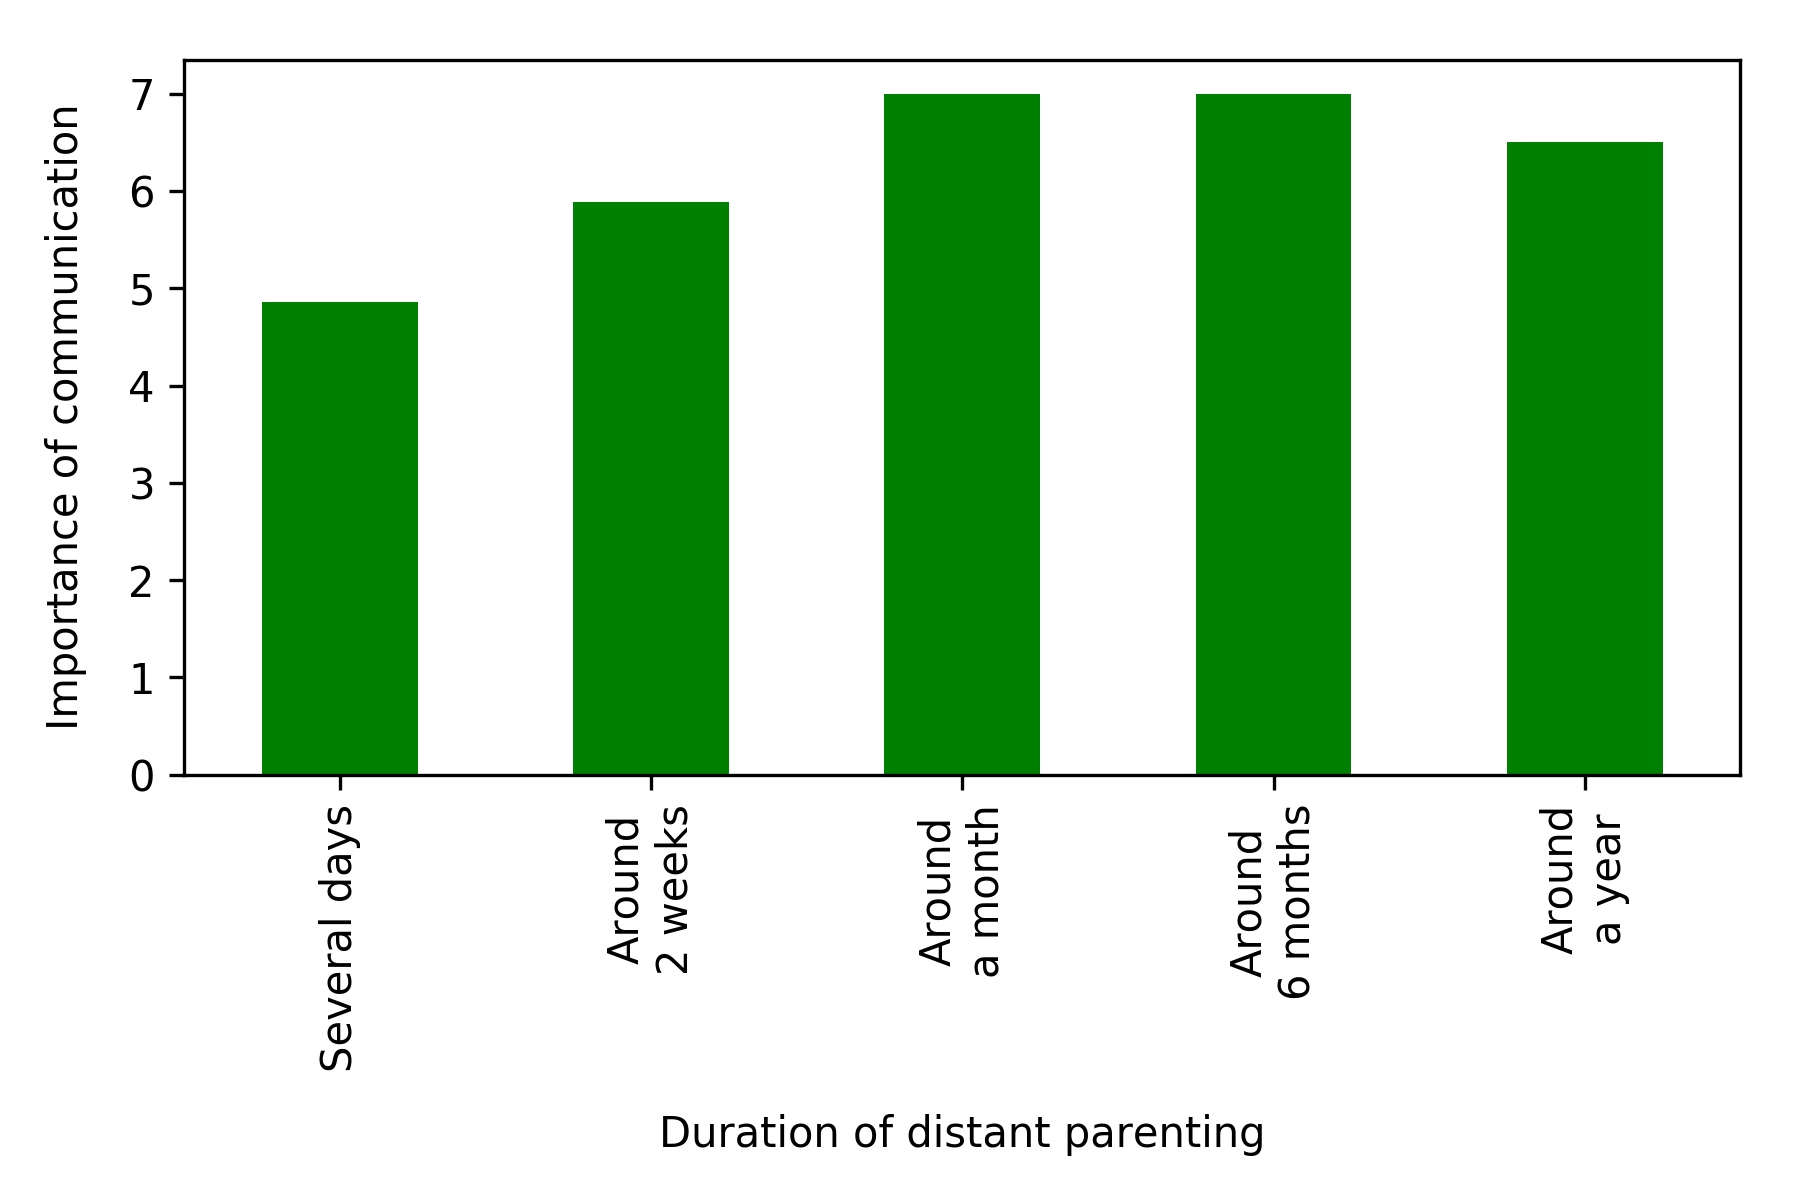
\includegraphics[scale=0.58]{plots/plot_5.png}
    \caption{Importance of communication from the parent point according to duration of distant-parenting experience}
    \label{fig:plot_5}
\end{figure}

\begin{figure}[h!]
    \centering
    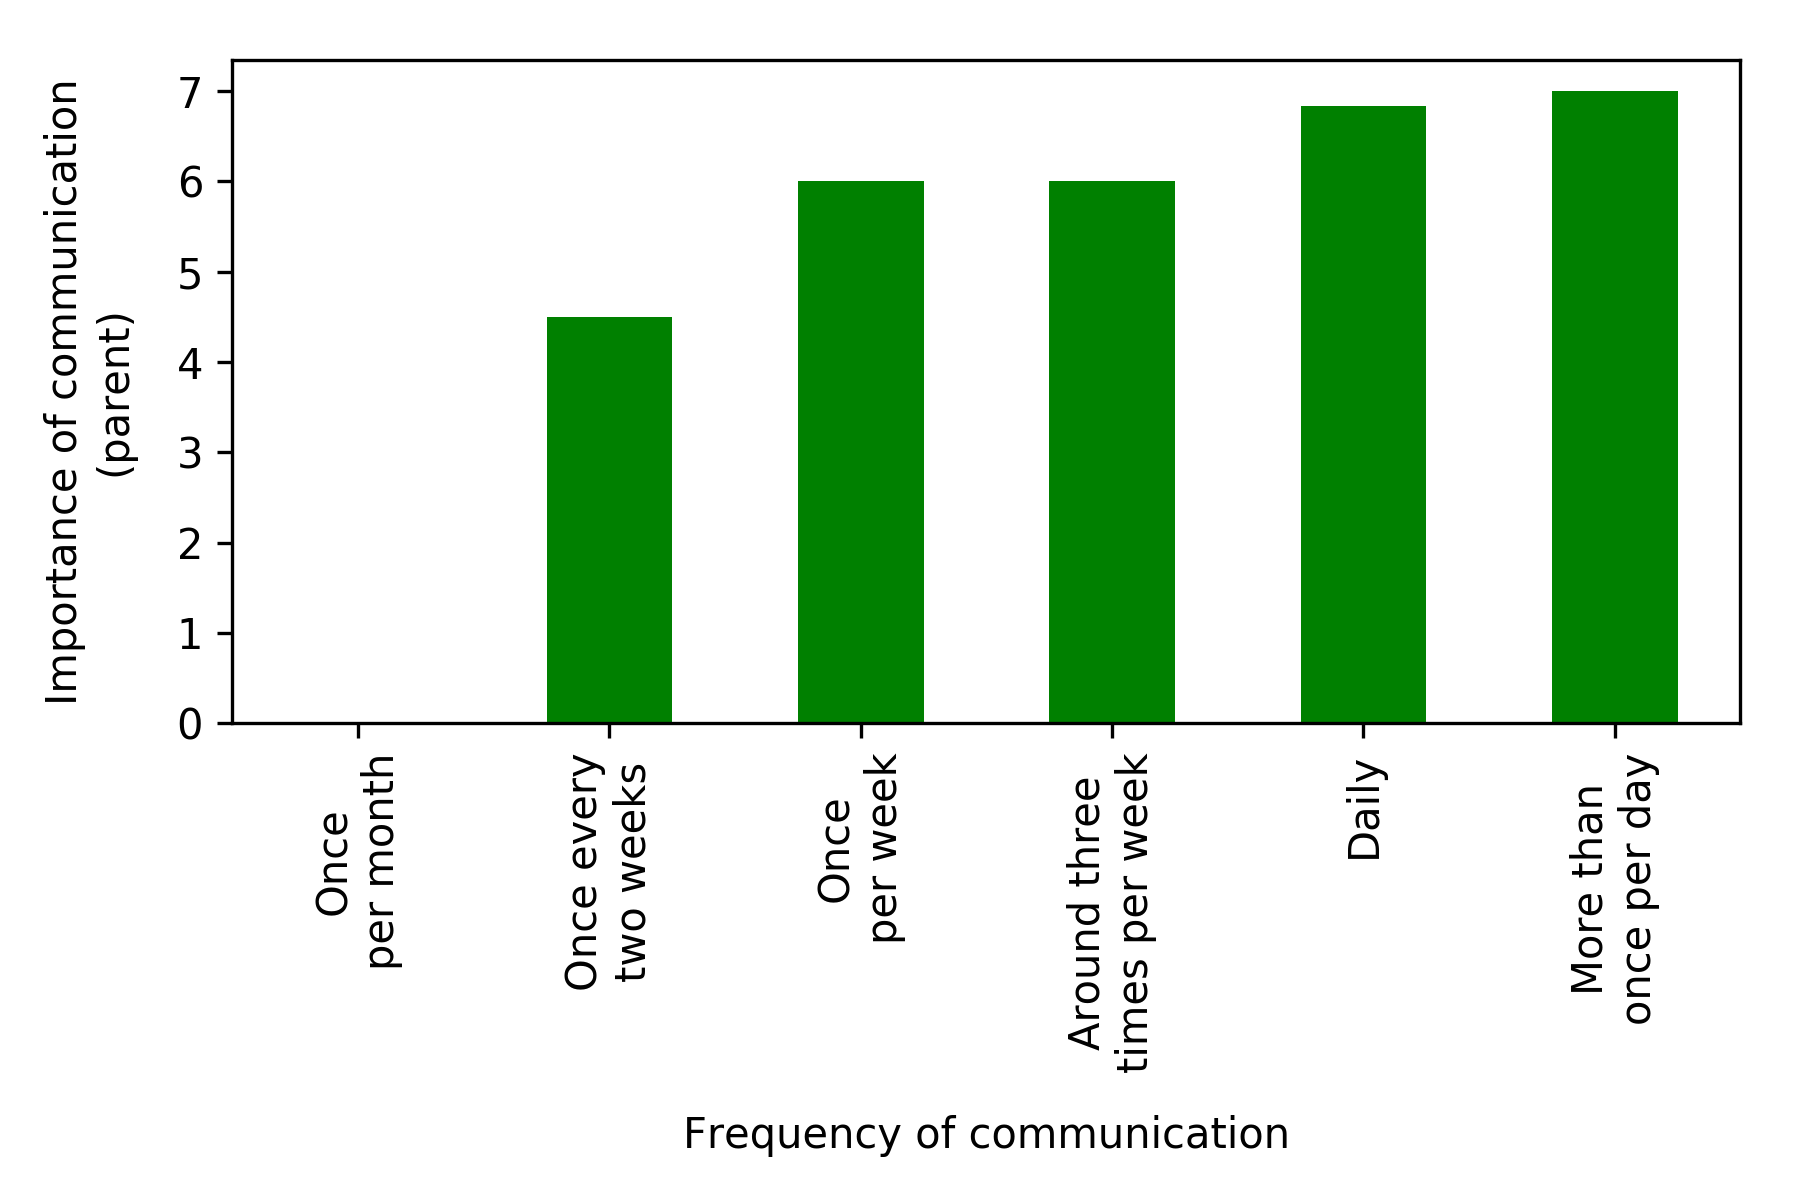
\includegraphics[scale=0.58]{plots/plot_8.png}
    \caption{Importance of communication from the parent point according to frequency of communication during distant-parenting experience}
    \label{fig:plot_8}
\end{figure}


\subsection{Interview protocol}
\label{appendix:interview_protocol}

The following interview protocol has been prepared for the research on “Communication Technologies for Left-Behind Children in Rural China”, in the scope of the “Global perspectives, local realities” SHS course. To continue our research on the Chinese field, by interviewing parents of left behind children, our assumptions could be tested and eventually further analyzed.

\vspace{4pt}
Please, fill in the missing informations as follows before starting the interview session:

Author: Matteo Yann Feo \& Simone Sanso

Session length: 40 minutes 

Participant Name: \hfill \_\_\_\_\_\_\_\_\_\_\_\_\_\_\_\_\_\_\_\_\_\_\_  $\leftarrow$ Fill in

Email: \hfill \_\_\_\_\_\_\_\_\_\_\_\_\_\_\_\_\_\_\_\_\_\_\_\_\_\_\_\_\_\_\_\_ $\leftarrow$ Fill in

Time/Date: \hfill \_\_\_\_\_\_\_\_\_\_\_\_\_\_\_\_\_\_\_\_\_\_\_\_\_\_\_\_ $\leftarrow$ Fill in

Location: \hfill \_\_\_\_\_\_\_\_\_\_\_\_\_\_\_\_\_\_\_\_\_\_\_\_\_\_\_\_\_ $\leftarrow$ Fill in

\vspace{6pt}
\subsubsection{Introduction \& Setup (5 mins)}

The session starts with a short introduction to what this interview is about, the context and the background for which it is being conducted. In the meantime, be sure that everything is setup correctly by double checking the following To-Do list:

\begin{todolist}
    \item Setup the recording tools and check if they work correctly.
    \item Prepare note-taking utilities, such as pen and paper.
    \item Verify the environment, being sure to have a relaxed location for the following 40 mins.
    \item In case a beverage is desired in the meantime, be sure to have it ready and available now.
    \item Be sure that your interviewed person has everything needed.
\end{todolist}

The introduction of the interview could be similar to the following one:

"Good morning and thank you for participating! I am Yann. I am studying at EPFL for a master degree in computer science. My main interest for this interview is to understand whether  a  technology  of  communication embedded in a smart toy could be helpful for parents distant from their children. During the interview, I will be having a conversation with you, asking questions that could help me to achieve my curiosity. In the meantime, my partner, will be assisting me by taking some notes. It is important to always remember that we are not evaluating you or your opinions in any way, there are no possible right and wrong answers that you could give. 
Here is how the session is going to proceed. Firstly, we'll break the ice by asking you a few general questions to know each other. We will record this interview, given your consent. We won't ever share this recording nor use it for anything else but pure support for this interview, so that I can go back and review things later to make sure we got everything right. Your name won't ever be linked to any result, so be relaxed and feel free to share your thoughts with us, without any troubles. Keep in mind that this is completely voluntary, the recording can be stopped whenever you want. Thus, if you don't like this idea, please let me know. 
How does all that sound to you? Do you have any questions at this point?"

\begin{todolist}
    \item Ask the interviewee to sign the written consent for recording purposes.
\end{todolist}

\vspace{2pt}
\subsubsection{Demographics \& Background (5 mins)}

This section will help us to create a background of the interviewee, while allowing him/her to start opening up to our questions. Use this session as a warming-up occasion to break the ice, while catching the first important features. Start to note down details on the interviewee, like gender, age, education level, marital status.

\begin{todolist}
    \item Tell us your name, and a little bit about yourself.
    \item Where do you come from?
    \item What is your occupation? Are you studying or working? In both cases, can you tell us something about it?
    \item Where are you currently living? Do you live with someone, or alone? 
\end{todolist}

\vspace{2pt}
\subsubsection{Main questions (20 mins)}

The following questions can be helpful to interpolate your impressions with the interviewee’s feelings and personal stories. Use them carefully as they might be intimidating for some people. Don’t forget to check for nonverbal behaviors, as they might be critical to have a complete idea of who you are interviewing, especially in this part. Note that the most important questions to be answered are marked with an asterisk (*).

\vspace{2pt}
(*) Pre-interview questions about their children :

\begin{todolist}
    \item How many children do you have?
    \item How old are they?
    \item What gender are they?
    \item Where do you they live?
    \item With who are they staying in your home village? (Lonely, with one of both parents, with grandparents or other relatives)
\end{todolist}

Main interview questions about the interviewed parent :

\begin{todolist}
    \item (*) How often and for how long do you come back home? 
    \item What is the main reason why you live far away from your children?
    \item How do you feel about this situation, not living with your children?
    \item Remember the last time you went back to your home village, how was the contact with your children? Was the meeting with your children as before you left them?
    \item During your childhood, have you ever experienced living far away from one of your parents? If yes, for how long? How did you live the situation? Could you tell us what was the main reason of your parent to out-migrate? How was the contact when meeting again with your parent? Could you communicate together, at that time, while being distant? (Check for non-verbal reactions while interviewee showcase personal experience)
    \item How common is your situation of distant parenting? Do you know any other persons in the same situation as you? How do they live it?
    \item (*) How would you define the importance of living with your children? In your case, is there a trade off between living with your children and having a job position? If yes, imagine that you could live in an ideal world, what would be the best solution? Would you rather work in your home village or be able to bring your children in town?
    \item (*) Do you own electronic devices? If yes, which ones? (Smartphone, computer, more…)
    \item (*) Do your children in your home village own electronic devices? If not, would they have the opportunity to use any? (Neighbourhood, school, etc.)
    \item (*) Do you use electronic devices to contact your children? If yes, how often? In general, are you calling your children when you have time? Or do they also get in touch with you, on their initiative?
    \item (*) From 0 to 7, how would you define the importance of communicating with your children? (0: insignificant, 4: neutral, 7: essential) (Check for non-verbal reactions while interviewee showcase personal experience)
\end{todolist}

\vspace{2pt}
\subsubsection{Interviewee's "show and tell" prototype (8 mins)}

This section is practical and allows us to showcase our project, related to the issue of distant parenting. In the context of CHIC (China Hardware Innovation Camp), a plush toy that encourages social interaction between parents and children, in a distant situation. It is a very resourceful moment, as it could bring additional and authentic feedback on a novel user scenario.

The explanation of the prototype could be similar to the following one:

"We have been working on this prototype. It is a plush toy that encourages social interaction, by having remotely turned on LEDs and sounds from a mobile application. Parents and children can therefore stay longer connected. Letting your children know when you think about them will help you stay 'toygether'\texttrademark."

Showcase the prototype and how it works with the mobile application.

\begin{todolist}
    \item What do you think about the idea?
    \item In your opinion, which are the positive and negative aspects?
    \item If you had the possibility to try this technology, would you be interested?
    \item What would you modify to improve it?
\end{todolist}

\vspace{2pt}
\subsubsection{Closing (2 mins)}

Thank the user at the end for participating to the session. Offer the possibility to ask any kind of question the interviewee might want to address you.  This is his/her time to wear the interviewer's shoes in your regards.

If the interviewee has no additional question, the interview is officially finished. Thank again your interviewee for the time and availability to participate to this session. Underline how useful his/her help has been for the project.
Turn off the recording tools only when you are completely sure that nothing will be added. It is important to not miss anything, so better have some extra recording to cut later.

Take some time to, directly after the end of the interview, write down some impressions you may have about the session. It is important to note down very early impressions about both verbal and physical languages, before they are forgotten. Those are the most authentic resources to get.




\subsection{List of contacts}
\label{appendix:contacts_list}
Below are listed all the contacts that have been reached, to spread as much as possible the survey.

\begin{itemize}
\item AFS programs for adolescents (15-18 years old): \\
Duration: 1 year \\
Kernstrasse 57, CH-8004 Zurich \\
Tel: +41 21 323 19 19 \\
Email: hello@afs.ch \\
https://www.afs.ch/fr/programmes-scolaires/ 

\vspace{4pt}
\item Canada-France exchange (16 years old): \\
Duration : 3 weeks \\
College of Jeanne d'Arc, 15 Rue du Chanoine Brun, 68100 Mulhouse, France \\
Tel: +33 3 89 45 36 31 \\
www.ejda.fr/ 

\vspace{4pt}
\item International exchange programs (14-18 years old): \\
Duration: 1 year \\
Rue Centrale 15, 1003 Lausanne \\
Tel: +41 800 822 811 \\
https://www.efswiss.ch/fr/highschool/ 

\vspace{4pt}
\item National observatory of the Erasmus + impact (1 year or 6 months): \\
Email: observatoire@agence-erasmus.fr \\
http://www.agence-erasmus.fr/page/observatoire/

\vspace{4pt}
\item Journal of international mobility:\\
Email: revue@agence-erasmus.fr \\
https://www.agence-erasmus.fr/page/JIM

\vspace{4pt}
\item Exchange program Brigitte Sauzay (14-17 years old): \\
Duration: 3 months in a host family in Germany and welcome 3 months in the family in France \\
https://www.ofaj.org/contact.html 

\vspace{4pt}
\item Internal exchanges and language stays in Switzerland (14-17 years old): \\
Duration: 1 year \\
College of Delémont, Avenue Station 7, 2800 Delémont \\
Tel: +41 32 421 00 70 \\
Email: info@coldel.org \\
http://www.college-delemont.ch/fr/Aide-aux-eleves/Echanges-et-sejours-linguistiques/Echanges-et-sejours-linguistiques.html \\
Cantonal manager of linguistic exchanges: \\
Patrice KAMBER, Pâquerettes 2, 2822 Courroux \\
- Prof: 032 435 65 92 / Private: 032 422 83 62 

\vspace{4pt}
\item Language Exchange and Mobility - DIP Geneva: \\
Catherine Fernandez Sonino: Head of Exchange \& Mobility DIP of the Cantonal Office for Language Exchange and Mobility \\
Chemin de l'Echo 5a, 1213 Onex \\
Email: catherine.fernandez@etat.ge.ch \\
Tel: +41 22 327 06 43, +41 79 175 56 46 \\
https://edu.ge.ch/site/elem/ 

\vspace{4pt}
\item Service of primary and secondary schools of Lausanne: \\
Place Chauderon 9, 5th floor, PO Box 5032, 1002 Lausanne \\
Tel: +41 21 315 64 11 - Fax: +41 21 315 60 04 \\
Email: seps@lausanne.ch \\
http://www.lausanne.ch/etablissements-scolaires/ 

\vspace{4pt}
\item Summer camp of Neuchatel:\\
Gisèle Nicaty \\
Quartier du Milieu 86, 2127 Les Bayards \\
Tel: +41 79 288 50 41, +41 32 866 17 29\\
Email: giroud.p-a@bluewin.ch\\
http://www.echanges-scolaires.com/index.php/fr/

\vspace{4pt}
\item Summer camp of the Grandes-Roches: \\
1348 le Brassus \\
Tel: +41 21 845 66 90 \\
Email: camps@asime.ch \\
http://www.grandesroches.ch/home 

\vspace{4pt}
\item Association of the Gros-de-Vaud Holiday Camp: \\
Mrs Florence Ethenoz \\
Chemin du Petit Record 60, 1040 Echallens \\
Tel: +41 21 881 10 76 \\
Email: info@colo-gros-de-vaud.ch \\
http://www.colo-gros-de-vaud.ch/clubdesk/www

\vspace{4pt}
\item Summer camp 4Fun: \\
Email: airfred@hotmail.com \\
http://4-fun.ch/ 

\vspace{4pt}
\item Summer camp CPV: \\
Swiss Village Street 14, PO Box 72, 1211 Geneva 8 \\
Tel: +41 22 809 49 79 \\
Email: info@camps.ch \\
http://www.camps.ch/fr/accueil 

\vspace{4pt}
\item Scouts of the Sacred Heart: \\
Jeanne Voruz \& Anne Thiébaud \\
Tel: +41 79 844 92 74 \& +41 79 284 50 38 \\
Email: cg@sacrescout.ch \\
http://www.sacrescout.ch/ 

\vspace{4pt}
\item Village Camps: \\
PO Box 1425, Rue de la Morache 14, 1260 Nyon 1 \\
Tel: +41 22 990 9400 \\
Email: camps@villagecamps.com \\
www.villagecamps.com

\vspace{4pt}
\item Alpadia Language Schools: \\
Grand-Rue 42, PO Box 1206, 1820 Montreux\\
Tel: +41 21 621 88 88\\
Email: info@alpadia.com\\
https://www.alpadia.com/fr/ 

\vspace{4pt}
\item Carol Panchaud Educom sàrl: \\
26 Route of Givrins, CH - 1276 Gingins\\
Tel: +41 22 776 69 15 \\
Email: carolpanchaud@educom.ch \\
http://educom.ch/fr

\vspace{4pt}
\item Caritas-Youth: \\
11, Jean-Violette Street, 1205 Geneva\\
Tel: +41 22 708 04 04\\
Email: info@caritas-jeunesse.ch\\
http://www.caritas-jeunesse.ch/

\vspace{4pt}
\item Holiday Camp St. Gervais: \\
CP 1337, 1211 Geneva 1\\
Tel: +41 78 896 71 84\\
Email: info@colonie-saint-gervais.ch\\
http://www.colonie-saint-gervais.ch/

\vspace{4pt}
\item Summer Camp of Ravoire - Camp Plein Soleil: \\
PO Box 87, CH-1920 Martigny 1\\
Email: info@camp-pleinsoleil.ch

\vspace{4pt}
\item Yverdon-les-Bains youth service and social cohesion: \\
Rue de Neuchâtel 2, 1400 Yverdon-les-Bains\\
Tel: +41 24 423 69 11\\
Email: vacances@yverdon-les-bains.ch\\
http://www.yverdon-les-bains.ch/prestations-deladministration/jeunesse-et-cohesion-sociale/enfanceetfamille/colonies-dete-et-dautomne/

\vspace{4pt}
\item fRilingue GmbH: \\
Stöckackerstrasse 93, 3018 Bern\\
Tel: +41 26 321 34 34 \\
Email: info@frilingue.com

\vspace{4pt}
\item Star Sports: \\
Path of Verger 2, PO Box 101, 1304 Cossonay-Ville\\
Tel: +41 79 356 44 61\\
Email: info@starsports.ch\\
http://www.starsports.ch/

\vspace{4pt}
\item Cap Loisirs Foundation: \\
34, Boulevard de Saint-Georges, 1205 Geneva\\
Tel: +41 22 731 86 00\\
Email: caploisirs@caploisirs.ch\\
http://www.caploisirs.ch/

\vspace{4pt}
\item SCE Holidays \& Events: \\
Rue de Lausanne 58, 1950 Sion\\
Tel: +41 79 693.33.64\\
Email: info@lescamps.ch\\
https://www.lescamps.ch/\\

\end{itemize}



% References of the Report
\thispagestyle{empty}
\vspace{1cm}
\begin{thebibliography}{9}
\addcontentsline{toc}{section}{References}

\bibitem{lab3-report} 
\textit{Lab 3.0 : Camera \& LCD conceptual design}. \\
CS-473 EPFL. Matteo Yann Feo \& Simone Aron Sanso. November 28th, 2017

\bibitem{lcd-controller} 
\textit{ILI9341 - a-Si TFT LCD Single Chip Driver 240RGBx320 Resolution and 262K color}. 
Rev. 1.11. ILI TECHNOLOGY CORP.

\bibitem{lcd-display} 
\textit{LT24 User Manual}. 
Altera. June 2015
 
\bibitem{avalon-interface} 
\textit{Avalon® Interface Specifications}.
MNL-AVABUSREF. Intel. May 2017.
 
\bibitem{fifo} 
\textit{Single- and Dual-Clock FIFO Megafunction}.
Rev. 4.0. Altera. May 2007.

\end{thebibliography}

\end{document}


\documentclass[a4paper,12pt]{article}

%% Layout
\usepackage[utf8]{inputenc}
\usepackage{palatino}
\usepackage[T1]{fontenc}
\usepackage[8pt]{extsizes}

\usepackage{geometry}
\geometry{
    a4paper,
    total={170mm,257mm},
    left=30mm,
    right=30mm,
    top=30mm,
    bottom=30mm,
 } 

%% Useful packages
\usepackage{amsmath}
\usepackage{amssymb}
\usepackage{mathtools}
\usepackage{microtype}

\usepackage[usenames, dvipsnames]{xcolor}
\usepackage{graphicx}
\usepackage{wrapfig}
\usepackage{subfig}
\usepackage{tabularx}
\usepackage{float}
\usepackage{caption}
\usepackage{multirow}
\usepackage{color, colortbl}
\usepackage{enumerate}

\usepackage{hyperref}
\usepackage{url}

\usepackage[english]{babel}
\usepackage{units}

\usepackage{textcomp}
\usepackage{titling}
\usepackage{blindtext}
\usepackage{listings}

\usepackage{braket}
\usepackage{rotating}

%\setlength{\droptitle}{-4em}     % Eliminate the default vertical space
%\addtolength{\droptitle}{-4pt}

\title{
    \centering
	
\includegraphics[width=0.5\textwidth]{images/Logo_EPFL.png}
    \\[1cm]
	\Huge China Hardware Innovation Camp\\[1cm]
    \huge Semester project report\\
    \rule{3.5cm}{0.9pt}\\[0.5cm]
    \huge HUM - 498 \vfill
    \normalsize
}

\author{
    \textbf{Laboratory group:}\\\\
    Chloe Dickson - \texttt{\href{mailto:chloe.dickson@epfl.ch}{simone.sanso@epfl.ch}} \\
    Matteo Yann Feo -    \texttt{\href{mailto:matteo.feo@epfl.ch}{matteo.feo@epfl.ch}} \\
    Simone Aron Sanso - \texttt{\href{mailto:simone.sanso@epfl.ch}{simone.sanso@epfl.ch}} \\\\
}

\date{\vfill \today}

\lstdefinestyle{Python}{
  language=Python,                % choose the language of the code
  numbers=left,                   % where to put the line-numbers
  stepnumber=1,                   % the step between two line-numbers.        
  numbersep=5pt,                  % how far the line-numbers are from the code
  backgroundcolor=\color{white},  % choose the background color. You must add \usepackage{color}
  showspaces=false,               % show spaces adding particular underscores
  showstringspaces=false,         % underline spaces within strings
  showtabs=false,                 % show tabs within strings adding particular underscores
  tabsize=2,                      % sets default tabsize to 2 spaces
  captionpos=b,                   % sets the caption-position to bottom
  breaklines=true,                % sets automatic line breaking
  breakatwhitespace=true,         % sets if automatic breaks should only happen at whitespace
  frame=single, 
  basicstyle=\ttfamily,
  keywordstyle=\color{Green}\bfseries,
  stringstyle=\color{red}\ttfamily,
  commentstyle=\color{OliveGreen}\ttfamily,
  %morecomment=[l][\color{magenta}]{\#}
}


\begin{document}
\maketitle
\thispagestyle{empty}

\newpage
\thispagestyle{empty}
\setcounter{page}{0}

\tableofcontents

\documentclass[a4paper,12pt]{article}

%% Layout
\usepackage[utf8]{inputenc}
\usepackage{palatino}
\usepackage[T1]{fontenc}
\usepackage[8pt]{extsizes}

\usepackage{geometry}
\geometry{
    a4paper,
    total={170mm,257mm},
    left=30mm,
    right=30mm,
    top=30mm,
    bottom=30mm,
 } 

%% Useful packages
\usepackage{amsmath}
\usepackage{amssymb}
\usepackage{mathtools}
\usepackage{microtype}

\usepackage[usenames, dvipsnames]{xcolor}
\usepackage{graphicx}
\usepackage{wrapfig}
\usepackage{subfig}
\usepackage{tabularx}
\usepackage{float}
\usepackage{caption}
\usepackage{multirow}
\usepackage{color, colortbl}
\usepackage{enumerate}

\usepackage{hyperref}
\usepackage{url}

\usepackage[english]{babel}
\usepackage{units}

\usepackage{textcomp}
\usepackage{titling}
\usepackage{blindtext}
\usepackage{listings}

\usepackage{braket}
\usepackage{rotating}

%\setlength{\droptitle}{-4em}     % Eliminate the default vertical space
%\addtolength{\droptitle}{-4pt}

\title{
    \centering
	
\includegraphics[width=0.5\textwidth]{images/Logo_EPFL.png}
    \\[1cm]
	\Huge China Hardware Innovation Camp\\[1cm]
    \huge Semester project report\\
    \rule{3.5cm}{0.9pt}\\[0.5cm]
    \huge HUM - 498 \vfill
    \normalsize
}

\author{
    \textbf{Laboratory group:}\\\\
    Chloe Dickson - \texttt{\href{mailto:chloe.dickson@epfl.ch}{simone.sanso@epfl.ch}} \\
    Matteo Yann Feo -    \texttt{\href{mailto:matteo.feo@epfl.ch}{matteo.feo@epfl.ch}} \\
    Simone Aron Sanso - \texttt{\href{mailto:simone.sanso@epfl.ch}{simone.sanso@epfl.ch}} \\\\
}

\date{\vfill \today}

\lstdefinestyle{Python}{
  language=Python,                % choose the language of the code
  numbers=left,                   % where to put the line-numbers
  stepnumber=1,                   % the step between two line-numbers.        
  numbersep=5pt,                  % how far the line-numbers are from the code
  backgroundcolor=\color{white},  % choose the background color. You must add \usepackage{color}
  showspaces=false,               % show spaces adding particular underscores
  showstringspaces=false,         % underline spaces within strings
  showtabs=false,                 % show tabs within strings adding particular underscores
  tabsize=2,                      % sets default tabsize to 2 spaces
  captionpos=b,                   % sets the caption-position to bottom
  breaklines=true,                % sets automatic line breaking
  breakatwhitespace=true,         % sets if automatic breaks should only happen at whitespace
  frame=single, 
  basicstyle=\ttfamily,
  keywordstyle=\color{Green}\bfseries,
  stringstyle=\color{red}\ttfamily,
  commentstyle=\color{OliveGreen}\ttfamily,
  %morecomment=[l][\color{magenta}]{\#}
}


\begin{document}
\maketitle
\thispagestyle{empty}

\newpage
\thispagestyle{empty}
\setcounter{page}{0}

\tableofcontents

\input{sections/1_introduction/main.tex}

\input{sections/2_structure/main.tex}
    \input{sections/2_structure/subsection_A.tex}
    \input{sections/2_structure/subsection_B.tex}
    \input{sections/2_structure/subsection_C.tex}
    
\input{sections/3_images_tables/main.tex}

\input{sections/4_code/main.tex}

\input{sections/5_conclusion/main.tex}

\input{appendix.tex}

\input{bibliography.tex}

\end{document}


\documentclass[a4paper,12pt]{article}

%% Layout
\usepackage[utf8]{inputenc}
\usepackage{palatino}
\usepackage[T1]{fontenc}
\usepackage[8pt]{extsizes}

\usepackage{geometry}
\geometry{
    a4paper,
    total={170mm,257mm},
    left=30mm,
    right=30mm,
    top=30mm,
    bottom=30mm,
 } 

%% Useful packages
\usepackage{amsmath}
\usepackage{amssymb}
\usepackage{mathtools}
\usepackage{microtype}

\usepackage[usenames, dvipsnames]{xcolor}
\usepackage{graphicx}
\usepackage{wrapfig}
\usepackage{subfig}
\usepackage{tabularx}
\usepackage{float}
\usepackage{caption}
\usepackage{multirow}
\usepackage{color, colortbl}
\usepackage{enumerate}

\usepackage{hyperref}
\usepackage{url}

\usepackage[english]{babel}
\usepackage{units}

\usepackage{textcomp}
\usepackage{titling}
\usepackage{blindtext}
\usepackage{listings}

\usepackage{braket}
\usepackage{rotating}

%\setlength{\droptitle}{-4em}     % Eliminate the default vertical space
%\addtolength{\droptitle}{-4pt}

\title{
    \centering
	
\includegraphics[width=0.5\textwidth]{images/Logo_EPFL.png}
    \\[1cm]
	\Huge China Hardware Innovation Camp\\[1cm]
    \huge Semester project report\\
    \rule{3.5cm}{0.9pt}\\[0.5cm]
    \huge HUM - 498 \vfill
    \normalsize
}

\author{
    \textbf{Laboratory group:}\\\\
    Chloe Dickson - \texttt{\href{mailto:chloe.dickson@epfl.ch}{simone.sanso@epfl.ch}} \\
    Matteo Yann Feo -    \texttt{\href{mailto:matteo.feo@epfl.ch}{matteo.feo@epfl.ch}} \\
    Simone Aron Sanso - \texttt{\href{mailto:simone.sanso@epfl.ch}{simone.sanso@epfl.ch}} \\\\
}

\date{\vfill \today}

\lstdefinestyle{Python}{
  language=Python,                % choose the language of the code
  numbers=left,                   % where to put the line-numbers
  stepnumber=1,                   % the step between two line-numbers.        
  numbersep=5pt,                  % how far the line-numbers are from the code
  backgroundcolor=\color{white},  % choose the background color. You must add \usepackage{color}
  showspaces=false,               % show spaces adding particular underscores
  showstringspaces=false,         % underline spaces within strings
  showtabs=false,                 % show tabs within strings adding particular underscores
  tabsize=2,                      % sets default tabsize to 2 spaces
  captionpos=b,                   % sets the caption-position to bottom
  breaklines=true,                % sets automatic line breaking
  breakatwhitespace=true,         % sets if automatic breaks should only happen at whitespace
  frame=single, 
  basicstyle=\ttfamily,
  keywordstyle=\color{Green}\bfseries,
  stringstyle=\color{red}\ttfamily,
  commentstyle=\color{OliveGreen}\ttfamily,
  %morecomment=[l][\color{magenta}]{\#}
}


\begin{document}
\maketitle
\thispagestyle{empty}

\newpage
\thispagestyle{empty}
\setcounter{page}{0}

\tableofcontents

\input{sections/1_introduction/main.tex}

\input{sections/2_structure/main.tex}
    \input{sections/2_structure/subsection_A.tex}
    \input{sections/2_structure/subsection_B.tex}
    \input{sections/2_structure/subsection_C.tex}
    
\input{sections/3_images_tables/main.tex}

\input{sections/4_code/main.tex}

\input{sections/5_conclusion/main.tex}

\input{appendix.tex}

\input{bibliography.tex}

\end{document}

    %\newpage
\subsection{Subsection A}
\label{subsec:A} 

This is the first subsection. I am saved into a file \textit{subsection\_A.tex} in the same folder as my main file. Pay attention to the format in the label tag in order to reference to the subsection elsewhere. The subsection is called in the main file of the whole document !

\medskip Nunc pulvinar, risus sed gravida pretium, eros tellus vehicula turpis, eget bibendum nisi dolor sed erat. Pellentesque sit amet orci sed ligula dictum cursus. Morbi gravida ligula sapien, non tristique orci semper id. Ut sollicitudin est ut nisi eleifend sollicitudin. Vivamus blandit congue risus id porttitor. Donec sed blandit mauris. Integer est leo, dapibus sed felis et, vulputate sagittis enim. Quisque eget purus vitae metus placerat rhoncus. Nulla eget lacus nec felis tincidunt suscipit ac eget tellus. Ut at augue fermentum, mattis justo sed, consectetur quam. Donec blandit euismod nisi ac auctor.
    %\newpage
\subsection{Subsection B}
\label{subsec:B} 

This is the second subsection. I am also saved into a file \textit{subsection\_B.tex} in the same folder as my main file. Pay attention to the format in the label tag in order to reference to the subsection elsewhere. The subsection is called in the main file of the whole document !

\medskip Nunc pulvinar, risus sed gravida pretium, eros tellus vehicula turpis, eget bibendum nisi dolor sed erat. Pellentesque sit amet orci sed ligula dictum cursus. Morbi gravida ligula sapien, non tristique orci semper id. Ut sollicitudin est ut nisi eleifend sollicitudin. Vivamus blandit congue risus id porttitor. Donec sed blandit mauris. Integer est leo, dapibus sed felis et, vulputate sagittis enim. Quisque eget purus vitae metus placerat rhoncus. Nulla eget lacus nec felis tincidunt suscipit ac eget tellus. Ut at augue fermentum, mattis justo sed, consectetur quam. Donec blandit euismod nisi ac auctor.
    %\newpage
\subsection{Subsection C}
\label{subsec:C} 

Okay, you got it by now ;-)
    
\documentclass[a4paper,12pt]{article}

%% Layout
\usepackage[utf8]{inputenc}
\usepackage{palatino}
\usepackage[T1]{fontenc}
\usepackage[8pt]{extsizes}

\usepackage{geometry}
\geometry{
    a4paper,
    total={170mm,257mm},
    left=30mm,
    right=30mm,
    top=30mm,
    bottom=30mm,
 } 

%% Useful packages
\usepackage{amsmath}
\usepackage{amssymb}
\usepackage{mathtools}
\usepackage{microtype}

\usepackage[usenames, dvipsnames]{xcolor}
\usepackage{graphicx}
\usepackage{wrapfig}
\usepackage{subfig}
\usepackage{tabularx}
\usepackage{float}
\usepackage{caption}
\usepackage{multirow}
\usepackage{color, colortbl}
\usepackage{enumerate}

\usepackage{hyperref}
\usepackage{url}

\usepackage[english]{babel}
\usepackage{units}

\usepackage{textcomp}
\usepackage{titling}
\usepackage{blindtext}
\usepackage{listings}

\usepackage{braket}
\usepackage{rotating}

%\setlength{\droptitle}{-4em}     % Eliminate the default vertical space
%\addtolength{\droptitle}{-4pt}

\title{
    \centering
	
\includegraphics[width=0.5\textwidth]{images/Logo_EPFL.png}
    \\[1cm]
	\Huge China Hardware Innovation Camp\\[1cm]
    \huge Semester project report\\
    \rule{3.5cm}{0.9pt}\\[0.5cm]
    \huge HUM - 498 \vfill
    \normalsize
}

\author{
    \textbf{Laboratory group:}\\\\
    Chloe Dickson - \texttt{\href{mailto:chloe.dickson@epfl.ch}{simone.sanso@epfl.ch}} \\
    Matteo Yann Feo -    \texttt{\href{mailto:matteo.feo@epfl.ch}{matteo.feo@epfl.ch}} \\
    Simone Aron Sanso - \texttt{\href{mailto:simone.sanso@epfl.ch}{simone.sanso@epfl.ch}} \\\\
}

\date{\vfill \today}

\lstdefinestyle{Python}{
  language=Python,                % choose the language of the code
  numbers=left,                   % where to put the line-numbers
  stepnumber=1,                   % the step between two line-numbers.        
  numbersep=5pt,                  % how far the line-numbers are from the code
  backgroundcolor=\color{white},  % choose the background color. You must add \usepackage{color}
  showspaces=false,               % show spaces adding particular underscores
  showstringspaces=false,         % underline spaces within strings
  showtabs=false,                 % show tabs within strings adding particular underscores
  tabsize=2,                      % sets default tabsize to 2 spaces
  captionpos=b,                   % sets the caption-position to bottom
  breaklines=true,                % sets automatic line breaking
  breakatwhitespace=true,         % sets if automatic breaks should only happen at whitespace
  frame=single, 
  basicstyle=\ttfamily,
  keywordstyle=\color{Green}\bfseries,
  stringstyle=\color{red}\ttfamily,
  commentstyle=\color{OliveGreen}\ttfamily,
  %morecomment=[l][\color{magenta}]{\#}
}


\begin{document}
\maketitle
\thispagestyle{empty}

\newpage
\thispagestyle{empty}
\setcounter{page}{0}

\tableofcontents

\input{sections/1_introduction/main.tex}

\input{sections/2_structure/main.tex}
    \input{sections/2_structure/subsection_A.tex}
    \input{sections/2_structure/subsection_B.tex}
    \input{sections/2_structure/subsection_C.tex}
    
\input{sections/3_images_tables/main.tex}

\input{sections/4_code/main.tex}

\input{sections/5_conclusion/main.tex}

\input{appendix.tex}

\input{bibliography.tex}

\end{document}


\documentclass[a4paper,12pt]{article}

%% Layout
\usepackage[utf8]{inputenc}
\usepackage{palatino}
\usepackage[T1]{fontenc}
\usepackage[8pt]{extsizes}

\usepackage{geometry}
\geometry{
    a4paper,
    total={170mm,257mm},
    left=30mm,
    right=30mm,
    top=30mm,
    bottom=30mm,
 } 

%% Useful packages
\usepackage{amsmath}
\usepackage{amssymb}
\usepackage{mathtools}
\usepackage{microtype}

\usepackage[usenames, dvipsnames]{xcolor}
\usepackage{graphicx}
\usepackage{wrapfig}
\usepackage{subfig}
\usepackage{tabularx}
\usepackage{float}
\usepackage{caption}
\usepackage{multirow}
\usepackage{color, colortbl}
\usepackage{enumerate}

\usepackage{hyperref}
\usepackage{url}

\usepackage[english]{babel}
\usepackage{units}

\usepackage{textcomp}
\usepackage{titling}
\usepackage{blindtext}
\usepackage{listings}

\usepackage{braket}
\usepackage{rotating}

%\setlength{\droptitle}{-4em}     % Eliminate the default vertical space
%\addtolength{\droptitle}{-4pt}

\title{
    \centering
	
\includegraphics[width=0.5\textwidth]{images/Logo_EPFL.png}
    \\[1cm]
	\Huge China Hardware Innovation Camp\\[1cm]
    \huge Semester project report\\
    \rule{3.5cm}{0.9pt}\\[0.5cm]
    \huge HUM - 498 \vfill
    \normalsize
}

\author{
    \textbf{Laboratory group:}\\\\
    Chloe Dickson - \texttt{\href{mailto:chloe.dickson@epfl.ch}{simone.sanso@epfl.ch}} \\
    Matteo Yann Feo -    \texttt{\href{mailto:matteo.feo@epfl.ch}{matteo.feo@epfl.ch}} \\
    Simone Aron Sanso - \texttt{\href{mailto:simone.sanso@epfl.ch}{simone.sanso@epfl.ch}} \\\\
}

\date{\vfill \today}

\lstdefinestyle{Python}{
  language=Python,                % choose the language of the code
  numbers=left,                   % where to put the line-numbers
  stepnumber=1,                   % the step between two line-numbers.        
  numbersep=5pt,                  % how far the line-numbers are from the code
  backgroundcolor=\color{white},  % choose the background color. You must add \usepackage{color}
  showspaces=false,               % show spaces adding particular underscores
  showstringspaces=false,         % underline spaces within strings
  showtabs=false,                 % show tabs within strings adding particular underscores
  tabsize=2,                      % sets default tabsize to 2 spaces
  captionpos=b,                   % sets the caption-position to bottom
  breaklines=true,                % sets automatic line breaking
  breakatwhitespace=true,         % sets if automatic breaks should only happen at whitespace
  frame=single, 
  basicstyle=\ttfamily,
  keywordstyle=\color{Green}\bfseries,
  stringstyle=\color{red}\ttfamily,
  commentstyle=\color{OliveGreen}\ttfamily,
  %morecomment=[l][\color{magenta}]{\#}
}


\begin{document}
\maketitle
\thispagestyle{empty}

\newpage
\thispagestyle{empty}
\setcounter{page}{0}

\tableofcontents

\input{sections/1_introduction/main.tex}

\input{sections/2_structure/main.tex}
    \input{sections/2_structure/subsection_A.tex}
    \input{sections/2_structure/subsection_B.tex}
    \input{sections/2_structure/subsection_C.tex}
    
\input{sections/3_images_tables/main.tex}

\input{sections/4_code/main.tex}

\input{sections/5_conclusion/main.tex}

\input{appendix.tex}

\input{bibliography.tex}

\end{document}


\documentclass[a4paper,12pt]{article}

%% Layout
\usepackage[utf8]{inputenc}
\usepackage{palatino}
\usepackage[T1]{fontenc}
\usepackage[8pt]{extsizes}

\usepackage{geometry}
\geometry{
    a4paper,
    total={170mm,257mm},
    left=30mm,
    right=30mm,
    top=30mm,
    bottom=30mm,
 } 

%% Useful packages
\usepackage{amsmath}
\usepackage{amssymb}
\usepackage{mathtools}
\usepackage{microtype}

\usepackage[usenames, dvipsnames]{xcolor}
\usepackage{graphicx}
\usepackage{wrapfig}
\usepackage{subfig}
\usepackage{tabularx}
\usepackage{float}
\usepackage{caption}
\usepackage{multirow}
\usepackage{color, colortbl}
\usepackage{enumerate}

\usepackage{hyperref}
\usepackage{url}

\usepackage[english]{babel}
\usepackage{units}

\usepackage{textcomp}
\usepackage{titling}
\usepackage{blindtext}
\usepackage{listings}

\usepackage{braket}
\usepackage{rotating}

%\setlength{\droptitle}{-4em}     % Eliminate the default vertical space
%\addtolength{\droptitle}{-4pt}

\title{
    \centering
	
\includegraphics[width=0.5\textwidth]{images/Logo_EPFL.png}
    \\[1cm]
	\Huge China Hardware Innovation Camp\\[1cm]
    \huge Semester project report\\
    \rule{3.5cm}{0.9pt}\\[0.5cm]
    \huge HUM - 498 \vfill
    \normalsize
}

\author{
    \textbf{Laboratory group:}\\\\
    Chloe Dickson - \texttt{\href{mailto:chloe.dickson@epfl.ch}{simone.sanso@epfl.ch}} \\
    Matteo Yann Feo -    \texttt{\href{mailto:matteo.feo@epfl.ch}{matteo.feo@epfl.ch}} \\
    Simone Aron Sanso - \texttt{\href{mailto:simone.sanso@epfl.ch}{simone.sanso@epfl.ch}} \\\\
}

\date{\vfill \today}

\lstdefinestyle{Python}{
  language=Python,                % choose the language of the code
  numbers=left,                   % where to put the line-numbers
  stepnumber=1,                   % the step between two line-numbers.        
  numbersep=5pt,                  % how far the line-numbers are from the code
  backgroundcolor=\color{white},  % choose the background color. You must add \usepackage{color}
  showspaces=false,               % show spaces adding particular underscores
  showstringspaces=false,         % underline spaces within strings
  showtabs=false,                 % show tabs within strings adding particular underscores
  tabsize=2,                      % sets default tabsize to 2 spaces
  captionpos=b,                   % sets the caption-position to bottom
  breaklines=true,                % sets automatic line breaking
  breakatwhitespace=true,         % sets if automatic breaks should only happen at whitespace
  frame=single, 
  basicstyle=\ttfamily,
  keywordstyle=\color{Green}\bfseries,
  stringstyle=\color{red}\ttfamily,
  commentstyle=\color{OliveGreen}\ttfamily,
  %morecomment=[l][\color{magenta}]{\#}
}


\begin{document}
\maketitle
\thispagestyle{empty}

\newpage
\thispagestyle{empty}
\setcounter{page}{0}

\tableofcontents

\input{sections/1_introduction/main.tex}

\input{sections/2_structure/main.tex}
    \input{sections/2_structure/subsection_A.tex}
    \input{sections/2_structure/subsection_B.tex}
    \input{sections/2_structure/subsection_C.tex}
    
\input{sections/3_images_tables/main.tex}

\input{sections/4_code/main.tex}

\input{sections/5_conclusion/main.tex}

\input{appendix.tex}

\input{bibliography.tex}

\end{document}


% Appendix of the Report
\appendix

In the following appendix are presented the questions of the survey (... a list of figures and tables) to the reader.

\subsection{Questions of the survey}
\label{appendix:survey_questions}
In this section is shown how the participants were questioned towards the survey. Only the questions in English will be shown here, skipping the French translations.

\medskip \textit{Form about communication technologies :} \\
Realizing a research project about social sciences within EPFL University (Lausanne), we would like to understand the importance of communication between parents and children, when they are at a distance during a continuous period of time.

\vspace{4pt}
1. In what language would like to answer this form?

2. To contextualize, we seek either :

- parents of a child having spent a period of time away from the household,

- children, teenagers and young adults having spent a period of time away from their family.

After having read the description above, do you qualify yourself as a parent or a child?

\vspace{4pt}
\noindent - If "parent" was selected question 2: 

3.a. Are you the mother or the father?

4.a. Have you already been separated from your child for at least 3 days? (Exchange semester abroad, holidays, summer camp, boy-scout, etc.)

5.a. If there were more than one experience of distance parenting, please consider the earliest one of them through the rest of the form (when you were the youngest). What is the reason why your child was distant from you? 

6.a. For how long have you been distant from your child?

7.a. How old was your child at that time?

8.a. What is your child's gender?

9.a. How often did you use a communication technology with your distant child? (Text messages, phone calls, video chat, etc.)

10.a. What kind of information did you seek from communicating with your distant child?

11.a. How would you define the importance of being able to communicate with your distant child?

\vspace{4pt}
\noindent - If "child" was selected question 2: 

3.b. Have you already been separated from your family for at least 3 days? (Exchange semester abroad, holidays, summer camp, boy-scout, etc.)

3.b. If there were more than one experience of separation from your family, please consider the earliest one of them through the rest of the form (when you were the youngest). What is the reason why you were distant from your family? 

4.b. For how long have you been away?

5.b. How old were you at that time?

6.b. What is your gender?

7.b. How often did you use a communication technology with your family? (Text messages, phone calls, video chat, etc.)

8.b. What kind of information did you seek from communicating with your family?

9.b. How would you define the importance of being able to communicate with your family?


\subsection{Additional plots of the results}
\label{appendix:additional-plots}

The following plots have been computed for the analysis of the data collected via the survey on distant-parenting. This appendix contains a set of plots that didn't need particular attention during the discussion, but can still be source of investigation.

\begin{figure}[h!]
    \centering
    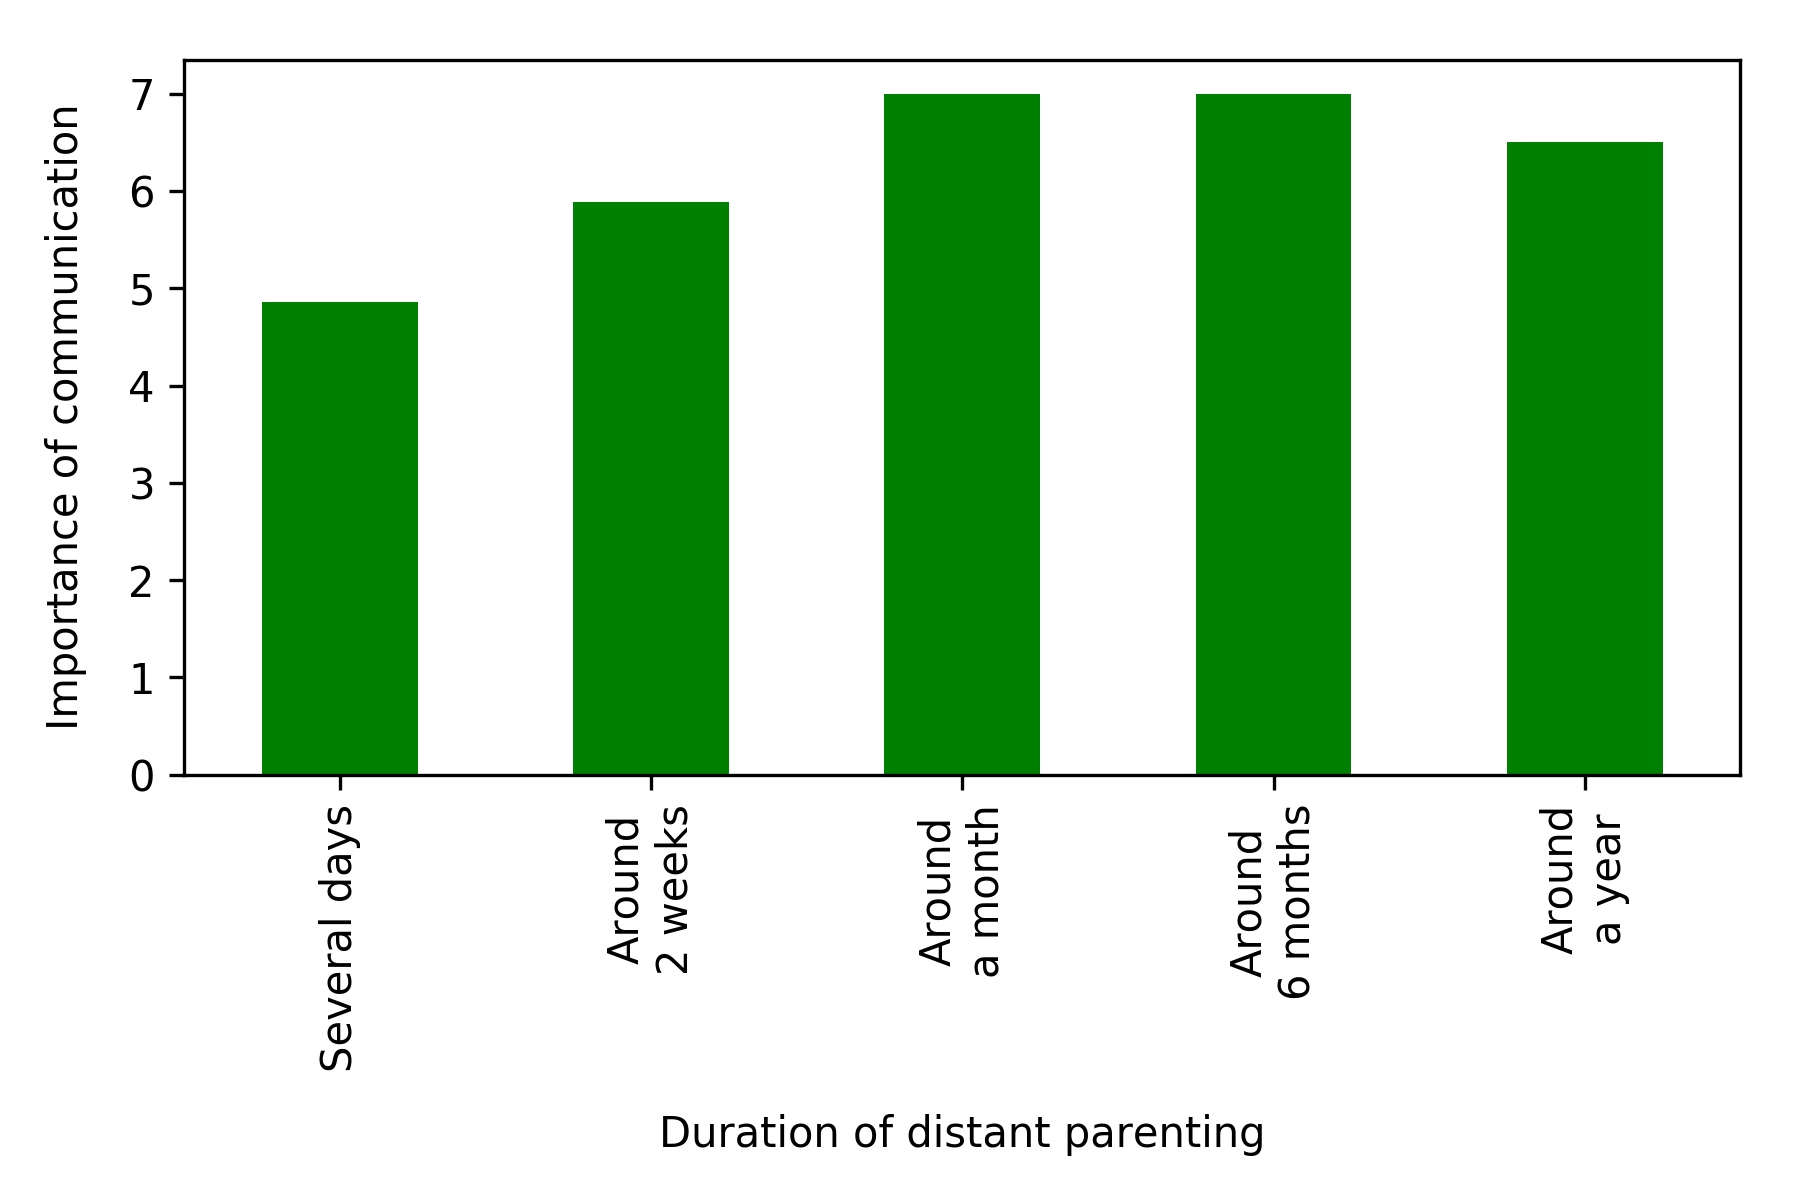
\includegraphics[scale=0.58]{plots/plot_5.png}
    \caption{Importance of communication from the parent point according to duration of distant-parenting experience}
    \label{fig:plot_5}
\end{figure}

\begin{figure}[h!]
    \centering
    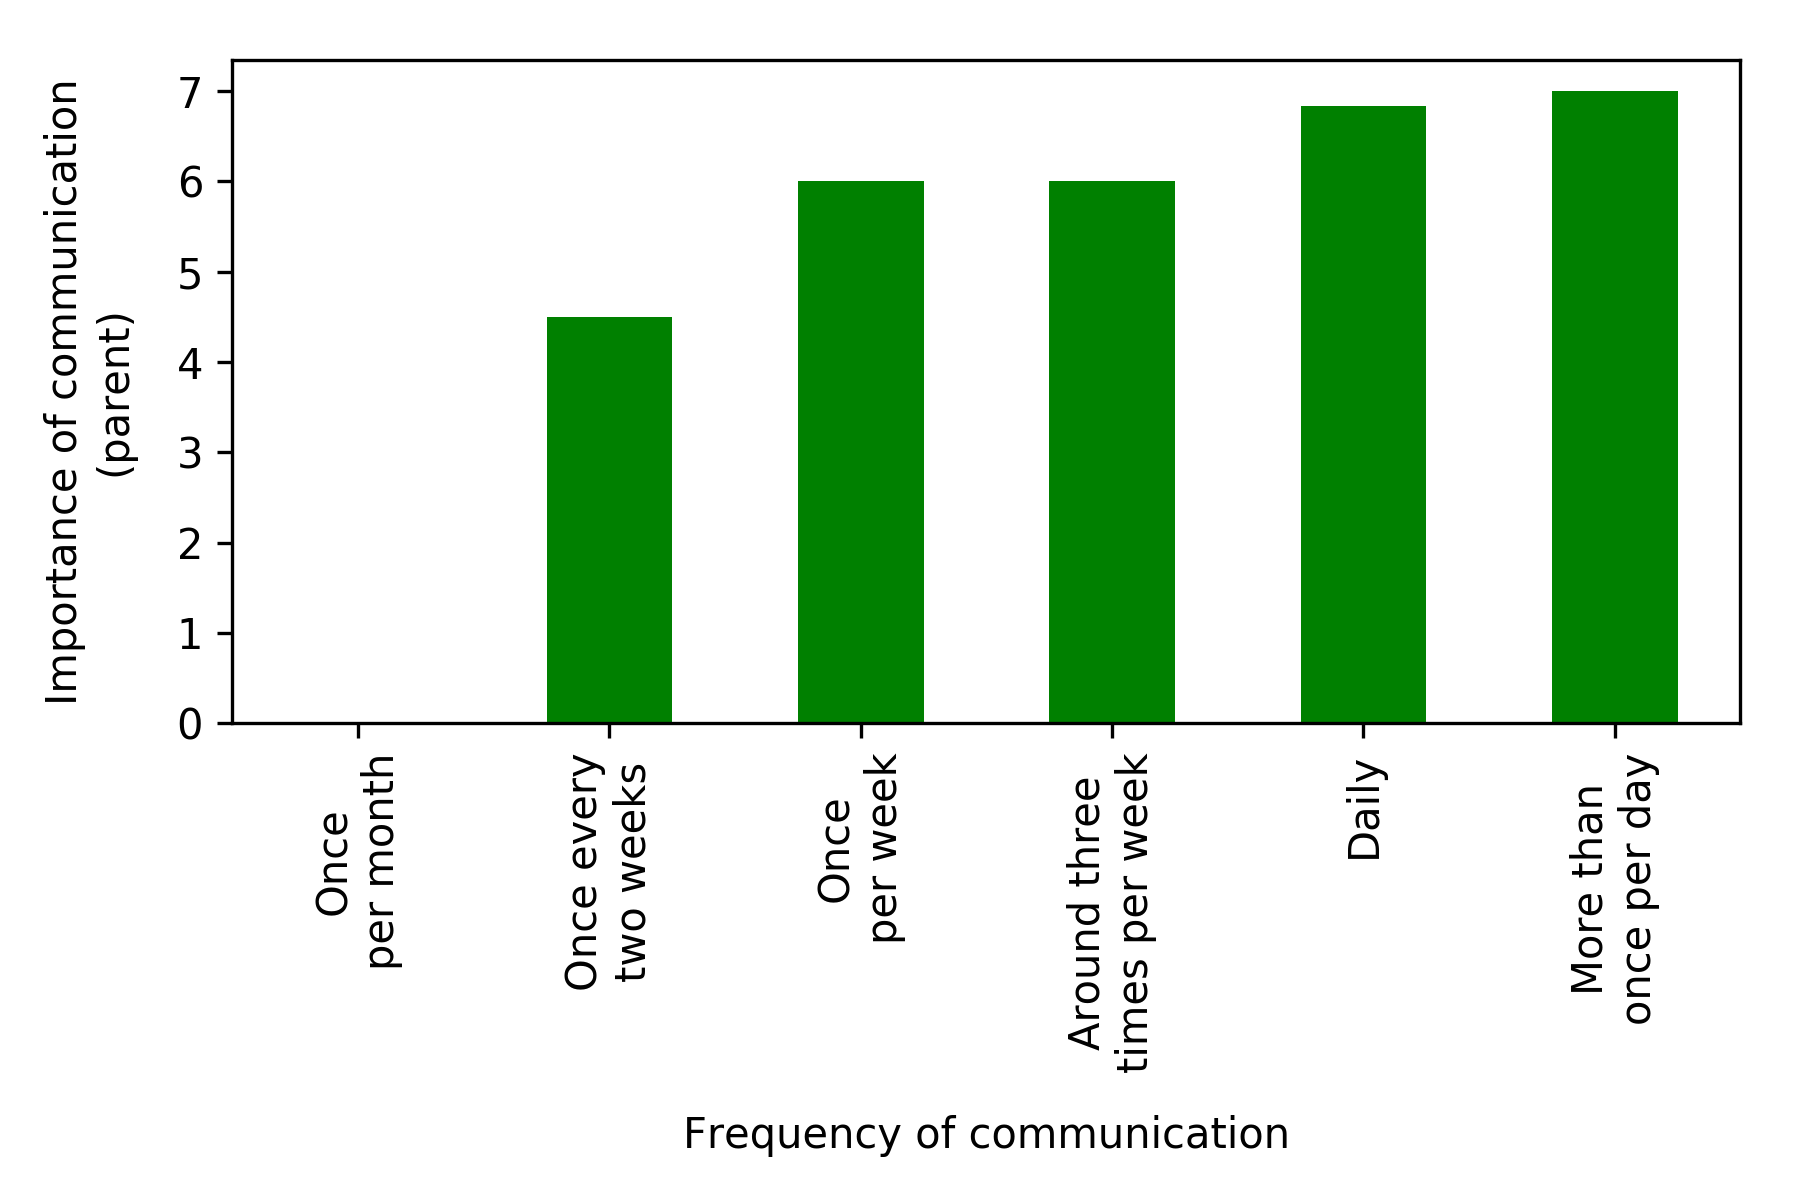
\includegraphics[scale=0.58]{plots/plot_8.png}
    \caption{Importance of communication from the parent point according to frequency of communication during distant-parenting experience}
    \label{fig:plot_8}
\end{figure}


\subsection{Interview protocol}
\label{appendix:interview_protocol}

The following interview protocol has been prepared for the research on “Communication Technologies for Left-Behind Children in Rural China”, in the scope of the “Global perspectives, local realities” SHS course. To continue our research on the Chinese field, by interviewing parents of left behind children, our assumptions could be tested and eventually further analyzed.

\vspace{4pt}
Please, fill in the missing informations as follows before starting the interview session:

Author: Matteo Yann Feo \& Simone Sanso

Session length: 40 minutes 

Participant Name: \hfill \_\_\_\_\_\_\_\_\_\_\_\_\_\_\_\_\_\_\_\_\_\_\_  $\leftarrow$ Fill in

Email: \hfill \_\_\_\_\_\_\_\_\_\_\_\_\_\_\_\_\_\_\_\_\_\_\_\_\_\_\_\_\_\_\_\_ $\leftarrow$ Fill in

Time/Date: \hfill \_\_\_\_\_\_\_\_\_\_\_\_\_\_\_\_\_\_\_\_\_\_\_\_\_\_\_\_ $\leftarrow$ Fill in

Location: \hfill \_\_\_\_\_\_\_\_\_\_\_\_\_\_\_\_\_\_\_\_\_\_\_\_\_\_\_\_\_ $\leftarrow$ Fill in

\vspace{6pt}
\subsubsection{Introduction \& Setup (5 mins)}

The session starts with a short introduction to what this interview is about, the context and the background for which it is being conducted. In the meantime, be sure that everything is setup correctly by double checking the following To-Do list:

\begin{todolist}
    \item Setup the recording tools and check if they work correctly.
    \item Prepare note-taking utilities, such as pen and paper.
    \item Verify the environment, being sure to have a relaxed location for the following 40 mins.
    \item In case a beverage is desired in the meantime, be sure to have it ready and available now.
    \item Be sure that your interviewed person has everything needed.
\end{todolist}

The introduction of the interview could be similar to the following one:

"Good morning and thank you for participating! I am Yann. I am studying at EPFL for a master degree in computer science. My main interest for this interview is to understand whether  a  technology  of  communication embedded in a smart toy could be helpful for parents distant from their children. During the interview, I will be having a conversation with you, asking questions that could help me to achieve my curiosity. In the meantime, my partner, will be assisting me by taking some notes. It is important to always remember that we are not evaluating you or your opinions in any way, there are no possible right and wrong answers that you could give. 
Here is how the session is going to proceed. Firstly, we'll break the ice by asking you a few general questions to know each other. We will record this interview, given your consent. We won't ever share this recording nor use it for anything else but pure support for this interview, so that I can go back and review things later to make sure we got everything right. Your name won't ever be linked to any result, so be relaxed and feel free to share your thoughts with us, without any troubles. Keep in mind that this is completely voluntary, the recording can be stopped whenever you want. Thus, if you don't like this idea, please let me know. 
How does all that sound to you? Do you have any questions at this point?"

\begin{todolist}
    \item Ask the interviewee to sign the written consent for recording purposes.
\end{todolist}

\vspace{2pt}
\subsubsection{Demographics \& Background (5 mins)}

This section will help us to create a background of the interviewee, while allowing him/her to start opening up to our questions. Use this session as a warming-up occasion to break the ice, while catching the first important features. Start to note down details on the interviewee, like gender, age, education level, marital status.

\begin{todolist}
    \item Tell us your name, and a little bit about yourself.
    \item Where do you come from?
    \item What is your occupation? Are you studying or working? In both cases, can you tell us something about it?
    \item Where are you currently living? Do you live with someone, or alone? 
\end{todolist}

\vspace{2pt}
\subsubsection{Main questions (20 mins)}

The following questions can be helpful to interpolate your impressions with the interviewee’s feelings and personal stories. Use them carefully as they might be intimidating for some people. Don’t forget to check for nonverbal behaviors, as they might be critical to have a complete idea of who you are interviewing, especially in this part. Note that the most important questions to be answered are marked with an asterisk (*).

\vspace{2pt}
(*) Pre-interview questions about their children :

\begin{todolist}
    \item How many children do you have?
    \item How old are they?
    \item What gender are they?
    \item Where do you they live?
    \item With who are they staying in your home village? (Lonely, with one of both parents, with grandparents or other relatives)
\end{todolist}

Main interview questions about the interviewed parent :

\begin{todolist}
    \item (*) How often and for how long do you come back home? 
    \item What is the main reason why you live far away from your children?
    \item How do you feel about this situation, not living with your children?
    \item Remember the last time you went back to your home village, how was the contact with your children? Was the meeting with your children as before you left them?
    \item During your childhood, have you ever experienced living far away from one of your parents? If yes, for how long? How did you live the situation? Could you tell us what was the main reason of your parent to out-migrate? How was the contact when meeting again with your parent? Could you communicate together, at that time, while being distant? (Check for non-verbal reactions while interviewee showcase personal experience)
    \item How common is your situation of distant parenting? Do you know any other persons in the same situation as you? How do they live it?
    \item (*) How would you define the importance of living with your children? In your case, is there a trade off between living with your children and having a job position? If yes, imagine that you could live in an ideal world, what would be the best solution? Would you rather work in your home village or be able to bring your children in town?
    \item (*) Do you own electronic devices? If yes, which ones? (Smartphone, computer, more…)
    \item (*) Do your children in your home village own electronic devices? If not, would they have the opportunity to use any? (Neighbourhood, school, etc.)
    \item (*) Do you use electronic devices to contact your children? If yes, how often? In general, are you calling your children when you have time? Or do they also get in touch with you, on their initiative?
    \item (*) From 0 to 7, how would you define the importance of communicating with your children? (0: insignificant, 4: neutral, 7: essential) (Check for non-verbal reactions while interviewee showcase personal experience)
\end{todolist}

\vspace{2pt}
\subsubsection{Interviewee's "show and tell" prototype (8 mins)}

This section is practical and allows us to showcase our project, related to the issue of distant parenting. In the context of CHIC (China Hardware Innovation Camp), a plush toy that encourages social interaction between parents and children, in a distant situation. It is a very resourceful moment, as it could bring additional and authentic feedback on a novel user scenario.

The explanation of the prototype could be similar to the following one:

"We have been working on this prototype. It is a plush toy that encourages social interaction, by having remotely turned on LEDs and sounds from a mobile application. Parents and children can therefore stay longer connected. Letting your children know when you think about them will help you stay 'toygether'\texttrademark."

Showcase the prototype and how it works with the mobile application.

\begin{todolist}
    \item What do you think about the idea?
    \item In your opinion, which are the positive and negative aspects?
    \item If you had the possibility to try this technology, would you be interested?
    \item What would you modify to improve it?
\end{todolist}

\vspace{2pt}
\subsubsection{Closing (2 mins)}

Thank the user at the end for participating to the session. Offer the possibility to ask any kind of question the interviewee might want to address you.  This is his/her time to wear the interviewer's shoes in your regards.

If the interviewee has no additional question, the interview is officially finished. Thank again your interviewee for the time and availability to participate to this session. Underline how useful his/her help has been for the project.
Turn off the recording tools only when you are completely sure that nothing will be added. It is important to not miss anything, so better have some extra recording to cut later.

Take some time to, directly after the end of the interview, write down some impressions you may have about the session. It is important to note down very early impressions about both verbal and physical languages, before they are forgotten. Those are the most authentic resources to get.




\subsection{List of contacts}
\label{appendix:contacts_list}
Below are listed all the contacts that have been reached, to spread as much as possible the survey.

\begin{itemize}
\item AFS programs for adolescents (15-18 years old): \\
Duration: 1 year \\
Kernstrasse 57, CH-8004 Zurich \\
Tel: +41 21 323 19 19 \\
Email: hello@afs.ch \\
https://www.afs.ch/fr/programmes-scolaires/ 

\vspace{4pt}
\item Canada-France exchange (16 years old): \\
Duration : 3 weeks \\
College of Jeanne d'Arc, 15 Rue du Chanoine Brun, 68100 Mulhouse, France \\
Tel: +33 3 89 45 36 31 \\
www.ejda.fr/ 

\vspace{4pt}
\item International exchange programs (14-18 years old): \\
Duration: 1 year \\
Rue Centrale 15, 1003 Lausanne \\
Tel: +41 800 822 811 \\
https://www.efswiss.ch/fr/highschool/ 

\vspace{4pt}
\item National observatory of the Erasmus + impact (1 year or 6 months): \\
Email: observatoire@agence-erasmus.fr \\
http://www.agence-erasmus.fr/page/observatoire/

\vspace{4pt}
\item Journal of international mobility:\\
Email: revue@agence-erasmus.fr \\
https://www.agence-erasmus.fr/page/JIM

\vspace{4pt}
\item Exchange program Brigitte Sauzay (14-17 years old): \\
Duration: 3 months in a host family in Germany and welcome 3 months in the family in France \\
https://www.ofaj.org/contact.html 

\vspace{4pt}
\item Internal exchanges and language stays in Switzerland (14-17 years old): \\
Duration: 1 year \\
College of Delémont, Avenue Station 7, 2800 Delémont \\
Tel: +41 32 421 00 70 \\
Email: info@coldel.org \\
http://www.college-delemont.ch/fr/Aide-aux-eleves/Echanges-et-sejours-linguistiques/Echanges-et-sejours-linguistiques.html \\
Cantonal manager of linguistic exchanges: \\
Patrice KAMBER, Pâquerettes 2, 2822 Courroux \\
- Prof: 032 435 65 92 / Private: 032 422 83 62 

\vspace{4pt}
\item Language Exchange and Mobility - DIP Geneva: \\
Catherine Fernandez Sonino: Head of Exchange \& Mobility DIP of the Cantonal Office for Language Exchange and Mobility \\
Chemin de l'Echo 5a, 1213 Onex \\
Email: catherine.fernandez@etat.ge.ch \\
Tel: +41 22 327 06 43, +41 79 175 56 46 \\
https://edu.ge.ch/site/elem/ 

\vspace{4pt}
\item Service of primary and secondary schools of Lausanne: \\
Place Chauderon 9, 5th floor, PO Box 5032, 1002 Lausanne \\
Tel: +41 21 315 64 11 - Fax: +41 21 315 60 04 \\
Email: seps@lausanne.ch \\
http://www.lausanne.ch/etablissements-scolaires/ 

\vspace{4pt}
\item Summer camp of Neuchatel:\\
Gisèle Nicaty \\
Quartier du Milieu 86, 2127 Les Bayards \\
Tel: +41 79 288 50 41, +41 32 866 17 29\\
Email: giroud.p-a@bluewin.ch\\
http://www.echanges-scolaires.com/index.php/fr/

\vspace{4pt}
\item Summer camp of the Grandes-Roches: \\
1348 le Brassus \\
Tel: +41 21 845 66 90 \\
Email: camps@asime.ch \\
http://www.grandesroches.ch/home 

\vspace{4pt}
\item Association of the Gros-de-Vaud Holiday Camp: \\
Mrs Florence Ethenoz \\
Chemin du Petit Record 60, 1040 Echallens \\
Tel: +41 21 881 10 76 \\
Email: info@colo-gros-de-vaud.ch \\
http://www.colo-gros-de-vaud.ch/clubdesk/www

\vspace{4pt}
\item Summer camp 4Fun: \\
Email: airfred@hotmail.com \\
http://4-fun.ch/ 

\vspace{4pt}
\item Summer camp CPV: \\
Swiss Village Street 14, PO Box 72, 1211 Geneva 8 \\
Tel: +41 22 809 49 79 \\
Email: info@camps.ch \\
http://www.camps.ch/fr/accueil 

\vspace{4pt}
\item Scouts of the Sacred Heart: \\
Jeanne Voruz \& Anne Thiébaud \\
Tel: +41 79 844 92 74 \& +41 79 284 50 38 \\
Email: cg@sacrescout.ch \\
http://www.sacrescout.ch/ 

\vspace{4pt}
\item Village Camps: \\
PO Box 1425, Rue de la Morache 14, 1260 Nyon 1 \\
Tel: +41 22 990 9400 \\
Email: camps@villagecamps.com \\
www.villagecamps.com

\vspace{4pt}
\item Alpadia Language Schools: \\
Grand-Rue 42, PO Box 1206, 1820 Montreux\\
Tel: +41 21 621 88 88\\
Email: info@alpadia.com\\
https://www.alpadia.com/fr/ 

\vspace{4pt}
\item Carol Panchaud Educom sàrl: \\
26 Route of Givrins, CH - 1276 Gingins\\
Tel: +41 22 776 69 15 \\
Email: carolpanchaud@educom.ch \\
http://educom.ch/fr

\vspace{4pt}
\item Caritas-Youth: \\
11, Jean-Violette Street, 1205 Geneva\\
Tel: +41 22 708 04 04\\
Email: info@caritas-jeunesse.ch\\
http://www.caritas-jeunesse.ch/

\vspace{4pt}
\item Holiday Camp St. Gervais: \\
CP 1337, 1211 Geneva 1\\
Tel: +41 78 896 71 84\\
Email: info@colonie-saint-gervais.ch\\
http://www.colonie-saint-gervais.ch/

\vspace{4pt}
\item Summer Camp of Ravoire - Camp Plein Soleil: \\
PO Box 87, CH-1920 Martigny 1\\
Email: info@camp-pleinsoleil.ch

\vspace{4pt}
\item Yverdon-les-Bains youth service and social cohesion: \\
Rue de Neuchâtel 2, 1400 Yverdon-les-Bains\\
Tel: +41 24 423 69 11\\
Email: vacances@yverdon-les-bains.ch\\
http://www.yverdon-les-bains.ch/prestations-deladministration/jeunesse-et-cohesion-sociale/enfanceetfamille/colonies-dete-et-dautomne/

\vspace{4pt}
\item fRilingue GmbH: \\
Stöckackerstrasse 93, 3018 Bern\\
Tel: +41 26 321 34 34 \\
Email: info@frilingue.com

\vspace{4pt}
\item Star Sports: \\
Path of Verger 2, PO Box 101, 1304 Cossonay-Ville\\
Tel: +41 79 356 44 61\\
Email: info@starsports.ch\\
http://www.starsports.ch/

\vspace{4pt}
\item Cap Loisirs Foundation: \\
34, Boulevard de Saint-Georges, 1205 Geneva\\
Tel: +41 22 731 86 00\\
Email: caploisirs@caploisirs.ch\\
http://www.caploisirs.ch/

\vspace{4pt}
\item SCE Holidays \& Events: \\
Rue de Lausanne 58, 1950 Sion\\
Tel: +41 79 693.33.64\\
Email: info@lescamps.ch\\
https://www.lescamps.ch/\\

\end{itemize}



% References of the Report
\thispagestyle{empty}
\vspace{1cm}
\begin{thebibliography}{9}
\addcontentsline{toc}{section}{References}

\bibitem{lab3-report} 
\textit{Lab 3.0 : Camera \& LCD conceptual design}. \\
CS-473 EPFL. Matteo Yann Feo \& Simone Aron Sanso. November 28th, 2017

\bibitem{lcd-controller} 
\textit{ILI9341 - a-Si TFT LCD Single Chip Driver 240RGBx320 Resolution and 262K color}. 
Rev. 1.11. ILI TECHNOLOGY CORP.

\bibitem{lcd-display} 
\textit{LT24 User Manual}. 
Altera. June 2015
 
\bibitem{avalon-interface} 
\textit{Avalon® Interface Specifications}.
MNL-AVABUSREF. Intel. May 2017.
 
\bibitem{fifo} 
\textit{Single- and Dual-Clock FIFO Megafunction}.
Rev. 4.0. Altera. May 2007.

\end{thebibliography}

\end{document}


\documentclass[a4paper,12pt]{article}

%% Layout
\usepackage[utf8]{inputenc}
\usepackage{palatino}
\usepackage[T1]{fontenc}
\usepackage[8pt]{extsizes}

\usepackage{geometry}
\geometry{
    a4paper,
    total={170mm,257mm},
    left=30mm,
    right=30mm,
    top=30mm,
    bottom=30mm,
 } 

%% Useful packages
\usepackage{amsmath}
\usepackage{amssymb}
\usepackage{mathtools}
\usepackage{microtype}

\usepackage[usenames, dvipsnames]{xcolor}
\usepackage{graphicx}
\usepackage{wrapfig}
\usepackage{subfig}
\usepackage{tabularx}
\usepackage{float}
\usepackage{caption}
\usepackage{multirow}
\usepackage{color, colortbl}
\usepackage{enumerate}

\usepackage{hyperref}
\usepackage{url}

\usepackage[english]{babel}
\usepackage{units}

\usepackage{textcomp}
\usepackage{titling}
\usepackage{blindtext}
\usepackage{listings}

\usepackage{braket}
\usepackage{rotating}

%\setlength{\droptitle}{-4em}     % Eliminate the default vertical space
%\addtolength{\droptitle}{-4pt}

\title{
    \centering
	
\includegraphics[width=0.5\textwidth]{images/Logo_EPFL.png}
    \\[1cm]
	\Huge China Hardware Innovation Camp\\[1cm]
    \huge Semester project report\\
    \rule{3.5cm}{0.9pt}\\[0.5cm]
    \huge HUM - 498 \vfill
    \normalsize
}

\author{
    \textbf{Laboratory group:}\\\\
    Chloe Dickson - \texttt{\href{mailto:chloe.dickson@epfl.ch}{simone.sanso@epfl.ch}} \\
    Matteo Yann Feo -    \texttt{\href{mailto:matteo.feo@epfl.ch}{matteo.feo@epfl.ch}} \\
    Simone Aron Sanso - \texttt{\href{mailto:simone.sanso@epfl.ch}{simone.sanso@epfl.ch}} \\\\
}

\date{\vfill \today}

\lstdefinestyle{Python}{
  language=Python,                % choose the language of the code
  numbers=left,                   % where to put the line-numbers
  stepnumber=1,                   % the step between two line-numbers.        
  numbersep=5pt,                  % how far the line-numbers are from the code
  backgroundcolor=\color{white},  % choose the background color. You must add \usepackage{color}
  showspaces=false,               % show spaces adding particular underscores
  showstringspaces=false,         % underline spaces within strings
  showtabs=false,                 % show tabs within strings adding particular underscores
  tabsize=2,                      % sets default tabsize to 2 spaces
  captionpos=b,                   % sets the caption-position to bottom
  breaklines=true,                % sets automatic line breaking
  breakatwhitespace=true,         % sets if automatic breaks should only happen at whitespace
  frame=single, 
  basicstyle=\ttfamily,
  keywordstyle=\color{Green}\bfseries,
  stringstyle=\color{red}\ttfamily,
  commentstyle=\color{OliveGreen}\ttfamily,
  %morecomment=[l][\color{magenta}]{\#}
}


\begin{document}
\maketitle
\thispagestyle{empty}

\newpage
\thispagestyle{empty}
\setcounter{page}{0}

\tableofcontents

\documentclass[a4paper,12pt]{article}

%% Layout
\usepackage[utf8]{inputenc}
\usepackage{palatino}
\usepackage[T1]{fontenc}
\usepackage[8pt]{extsizes}

\usepackage{geometry}
\geometry{
    a4paper,
    total={170mm,257mm},
    left=30mm,
    right=30mm,
    top=30mm,
    bottom=30mm,
 } 

%% Useful packages
\usepackage{amsmath}
\usepackage{amssymb}
\usepackage{mathtools}
\usepackage{microtype}

\usepackage[usenames, dvipsnames]{xcolor}
\usepackage{graphicx}
\usepackage{wrapfig}
\usepackage{subfig}
\usepackage{tabularx}
\usepackage{float}
\usepackage{caption}
\usepackage{multirow}
\usepackage{color, colortbl}
\usepackage{enumerate}

\usepackage{hyperref}
\usepackage{url}

\usepackage[english]{babel}
\usepackage{units}

\usepackage{textcomp}
\usepackage{titling}
\usepackage{blindtext}
\usepackage{listings}

\usepackage{braket}
\usepackage{rotating}

%\setlength{\droptitle}{-4em}     % Eliminate the default vertical space
%\addtolength{\droptitle}{-4pt}

\title{
    \centering
	
\includegraphics[width=0.5\textwidth]{images/Logo_EPFL.png}
    \\[1cm]
	\Huge China Hardware Innovation Camp\\[1cm]
    \huge Semester project report\\
    \rule{3.5cm}{0.9pt}\\[0.5cm]
    \huge HUM - 498 \vfill
    \normalsize
}

\author{
    \textbf{Laboratory group:}\\\\
    Chloe Dickson - \texttt{\href{mailto:chloe.dickson@epfl.ch}{simone.sanso@epfl.ch}} \\
    Matteo Yann Feo -    \texttt{\href{mailto:matteo.feo@epfl.ch}{matteo.feo@epfl.ch}} \\
    Simone Aron Sanso - \texttt{\href{mailto:simone.sanso@epfl.ch}{simone.sanso@epfl.ch}} \\\\
}

\date{\vfill \today}

\lstdefinestyle{Python}{
  language=Python,                % choose the language of the code
  numbers=left,                   % where to put the line-numbers
  stepnumber=1,                   % the step between two line-numbers.        
  numbersep=5pt,                  % how far the line-numbers are from the code
  backgroundcolor=\color{white},  % choose the background color. You must add \usepackage{color}
  showspaces=false,               % show spaces adding particular underscores
  showstringspaces=false,         % underline spaces within strings
  showtabs=false,                 % show tabs within strings adding particular underscores
  tabsize=2,                      % sets default tabsize to 2 spaces
  captionpos=b,                   % sets the caption-position to bottom
  breaklines=true,                % sets automatic line breaking
  breakatwhitespace=true,         % sets if automatic breaks should only happen at whitespace
  frame=single, 
  basicstyle=\ttfamily,
  keywordstyle=\color{Green}\bfseries,
  stringstyle=\color{red}\ttfamily,
  commentstyle=\color{OliveGreen}\ttfamily,
  %morecomment=[l][\color{magenta}]{\#}
}


\begin{document}
\maketitle
\thispagestyle{empty}

\newpage
\thispagestyle{empty}
\setcounter{page}{0}

\tableofcontents

\input{sections/1_introduction/main.tex}

\input{sections/2_structure/main.tex}
    \input{sections/2_structure/subsection_A.tex}
    \input{sections/2_structure/subsection_B.tex}
    \input{sections/2_structure/subsection_C.tex}
    
\input{sections/3_images_tables/main.tex}

\input{sections/4_code/main.tex}

\input{sections/5_conclusion/main.tex}

\input{appendix.tex}

\input{bibliography.tex}

\end{document}


\documentclass[a4paper,12pt]{article}

%% Layout
\usepackage[utf8]{inputenc}
\usepackage{palatino}
\usepackage[T1]{fontenc}
\usepackage[8pt]{extsizes}

\usepackage{geometry}
\geometry{
    a4paper,
    total={170mm,257mm},
    left=30mm,
    right=30mm,
    top=30mm,
    bottom=30mm,
 } 

%% Useful packages
\usepackage{amsmath}
\usepackage{amssymb}
\usepackage{mathtools}
\usepackage{microtype}

\usepackage[usenames, dvipsnames]{xcolor}
\usepackage{graphicx}
\usepackage{wrapfig}
\usepackage{subfig}
\usepackage{tabularx}
\usepackage{float}
\usepackage{caption}
\usepackage{multirow}
\usepackage{color, colortbl}
\usepackage{enumerate}

\usepackage{hyperref}
\usepackage{url}

\usepackage[english]{babel}
\usepackage{units}

\usepackage{textcomp}
\usepackage{titling}
\usepackage{blindtext}
\usepackage{listings}

\usepackage{braket}
\usepackage{rotating}

%\setlength{\droptitle}{-4em}     % Eliminate the default vertical space
%\addtolength{\droptitle}{-4pt}

\title{
    \centering
	
\includegraphics[width=0.5\textwidth]{images/Logo_EPFL.png}
    \\[1cm]
	\Huge China Hardware Innovation Camp\\[1cm]
    \huge Semester project report\\
    \rule{3.5cm}{0.9pt}\\[0.5cm]
    \huge HUM - 498 \vfill
    \normalsize
}

\author{
    \textbf{Laboratory group:}\\\\
    Chloe Dickson - \texttt{\href{mailto:chloe.dickson@epfl.ch}{simone.sanso@epfl.ch}} \\
    Matteo Yann Feo -    \texttt{\href{mailto:matteo.feo@epfl.ch}{matteo.feo@epfl.ch}} \\
    Simone Aron Sanso - \texttt{\href{mailto:simone.sanso@epfl.ch}{simone.sanso@epfl.ch}} \\\\
}

\date{\vfill \today}

\lstdefinestyle{Python}{
  language=Python,                % choose the language of the code
  numbers=left,                   % where to put the line-numbers
  stepnumber=1,                   % the step between two line-numbers.        
  numbersep=5pt,                  % how far the line-numbers are from the code
  backgroundcolor=\color{white},  % choose the background color. You must add \usepackage{color}
  showspaces=false,               % show spaces adding particular underscores
  showstringspaces=false,         % underline spaces within strings
  showtabs=false,                 % show tabs within strings adding particular underscores
  tabsize=2,                      % sets default tabsize to 2 spaces
  captionpos=b,                   % sets the caption-position to bottom
  breaklines=true,                % sets automatic line breaking
  breakatwhitespace=true,         % sets if automatic breaks should only happen at whitespace
  frame=single, 
  basicstyle=\ttfamily,
  keywordstyle=\color{Green}\bfseries,
  stringstyle=\color{red}\ttfamily,
  commentstyle=\color{OliveGreen}\ttfamily,
  %morecomment=[l][\color{magenta}]{\#}
}


\begin{document}
\maketitle
\thispagestyle{empty}

\newpage
\thispagestyle{empty}
\setcounter{page}{0}

\tableofcontents

\input{sections/1_introduction/main.tex}

\input{sections/2_structure/main.tex}
    \input{sections/2_structure/subsection_A.tex}
    \input{sections/2_structure/subsection_B.tex}
    \input{sections/2_structure/subsection_C.tex}
    
\input{sections/3_images_tables/main.tex}

\input{sections/4_code/main.tex}

\input{sections/5_conclusion/main.tex}

\input{appendix.tex}

\input{bibliography.tex}

\end{document}

    %\newpage
\subsection{Subsection A}
\label{subsec:A} 

This is the first subsection. I am saved into a file \textit{subsection\_A.tex} in the same folder as my main file. Pay attention to the format in the label tag in order to reference to the subsection elsewhere. The subsection is called in the main file of the whole document !

\medskip Nunc pulvinar, risus sed gravida pretium, eros tellus vehicula turpis, eget bibendum nisi dolor sed erat. Pellentesque sit amet orci sed ligula dictum cursus. Morbi gravida ligula sapien, non tristique orci semper id. Ut sollicitudin est ut nisi eleifend sollicitudin. Vivamus blandit congue risus id porttitor. Donec sed blandit mauris. Integer est leo, dapibus sed felis et, vulputate sagittis enim. Quisque eget purus vitae metus placerat rhoncus. Nulla eget lacus nec felis tincidunt suscipit ac eget tellus. Ut at augue fermentum, mattis justo sed, consectetur quam. Donec blandit euismod nisi ac auctor.
    %\newpage
\subsection{Subsection B}
\label{subsec:B} 

This is the second subsection. I am also saved into a file \textit{subsection\_B.tex} in the same folder as my main file. Pay attention to the format in the label tag in order to reference to the subsection elsewhere. The subsection is called in the main file of the whole document !

\medskip Nunc pulvinar, risus sed gravida pretium, eros tellus vehicula turpis, eget bibendum nisi dolor sed erat. Pellentesque sit amet orci sed ligula dictum cursus. Morbi gravida ligula sapien, non tristique orci semper id. Ut sollicitudin est ut nisi eleifend sollicitudin. Vivamus blandit congue risus id porttitor. Donec sed blandit mauris. Integer est leo, dapibus sed felis et, vulputate sagittis enim. Quisque eget purus vitae metus placerat rhoncus. Nulla eget lacus nec felis tincidunt suscipit ac eget tellus. Ut at augue fermentum, mattis justo sed, consectetur quam. Donec blandit euismod nisi ac auctor.
    %\newpage
\subsection{Subsection C}
\label{subsec:C} 

Okay, you got it by now ;-)
    
\documentclass[a4paper,12pt]{article}

%% Layout
\usepackage[utf8]{inputenc}
\usepackage{palatino}
\usepackage[T1]{fontenc}
\usepackage[8pt]{extsizes}

\usepackage{geometry}
\geometry{
    a4paper,
    total={170mm,257mm},
    left=30mm,
    right=30mm,
    top=30mm,
    bottom=30mm,
 } 

%% Useful packages
\usepackage{amsmath}
\usepackage{amssymb}
\usepackage{mathtools}
\usepackage{microtype}

\usepackage[usenames, dvipsnames]{xcolor}
\usepackage{graphicx}
\usepackage{wrapfig}
\usepackage{subfig}
\usepackage{tabularx}
\usepackage{float}
\usepackage{caption}
\usepackage{multirow}
\usepackage{color, colortbl}
\usepackage{enumerate}

\usepackage{hyperref}
\usepackage{url}

\usepackage[english]{babel}
\usepackage{units}

\usepackage{textcomp}
\usepackage{titling}
\usepackage{blindtext}
\usepackage{listings}

\usepackage{braket}
\usepackage{rotating}

%\setlength{\droptitle}{-4em}     % Eliminate the default vertical space
%\addtolength{\droptitle}{-4pt}

\title{
    \centering
	
\includegraphics[width=0.5\textwidth]{images/Logo_EPFL.png}
    \\[1cm]
	\Huge China Hardware Innovation Camp\\[1cm]
    \huge Semester project report\\
    \rule{3.5cm}{0.9pt}\\[0.5cm]
    \huge HUM - 498 \vfill
    \normalsize
}

\author{
    \textbf{Laboratory group:}\\\\
    Chloe Dickson - \texttt{\href{mailto:chloe.dickson@epfl.ch}{simone.sanso@epfl.ch}} \\
    Matteo Yann Feo -    \texttt{\href{mailto:matteo.feo@epfl.ch}{matteo.feo@epfl.ch}} \\
    Simone Aron Sanso - \texttt{\href{mailto:simone.sanso@epfl.ch}{simone.sanso@epfl.ch}} \\\\
}

\date{\vfill \today}

\lstdefinestyle{Python}{
  language=Python,                % choose the language of the code
  numbers=left,                   % where to put the line-numbers
  stepnumber=1,                   % the step between two line-numbers.        
  numbersep=5pt,                  % how far the line-numbers are from the code
  backgroundcolor=\color{white},  % choose the background color. You must add \usepackage{color}
  showspaces=false,               % show spaces adding particular underscores
  showstringspaces=false,         % underline spaces within strings
  showtabs=false,                 % show tabs within strings adding particular underscores
  tabsize=2,                      % sets default tabsize to 2 spaces
  captionpos=b,                   % sets the caption-position to bottom
  breaklines=true,                % sets automatic line breaking
  breakatwhitespace=true,         % sets if automatic breaks should only happen at whitespace
  frame=single, 
  basicstyle=\ttfamily,
  keywordstyle=\color{Green}\bfseries,
  stringstyle=\color{red}\ttfamily,
  commentstyle=\color{OliveGreen}\ttfamily,
  %morecomment=[l][\color{magenta}]{\#}
}


\begin{document}
\maketitle
\thispagestyle{empty}

\newpage
\thispagestyle{empty}
\setcounter{page}{0}

\tableofcontents

\input{sections/1_introduction/main.tex}

\input{sections/2_structure/main.tex}
    \input{sections/2_structure/subsection_A.tex}
    \input{sections/2_structure/subsection_B.tex}
    \input{sections/2_structure/subsection_C.tex}
    
\input{sections/3_images_tables/main.tex}

\input{sections/4_code/main.tex}

\input{sections/5_conclusion/main.tex}

\input{appendix.tex}

\input{bibliography.tex}

\end{document}


\documentclass[a4paper,12pt]{article}

%% Layout
\usepackage[utf8]{inputenc}
\usepackage{palatino}
\usepackage[T1]{fontenc}
\usepackage[8pt]{extsizes}

\usepackage{geometry}
\geometry{
    a4paper,
    total={170mm,257mm},
    left=30mm,
    right=30mm,
    top=30mm,
    bottom=30mm,
 } 

%% Useful packages
\usepackage{amsmath}
\usepackage{amssymb}
\usepackage{mathtools}
\usepackage{microtype}

\usepackage[usenames, dvipsnames]{xcolor}
\usepackage{graphicx}
\usepackage{wrapfig}
\usepackage{subfig}
\usepackage{tabularx}
\usepackage{float}
\usepackage{caption}
\usepackage{multirow}
\usepackage{color, colortbl}
\usepackage{enumerate}

\usepackage{hyperref}
\usepackage{url}

\usepackage[english]{babel}
\usepackage{units}

\usepackage{textcomp}
\usepackage{titling}
\usepackage{blindtext}
\usepackage{listings}

\usepackage{braket}
\usepackage{rotating}

%\setlength{\droptitle}{-4em}     % Eliminate the default vertical space
%\addtolength{\droptitle}{-4pt}

\title{
    \centering
	
\includegraphics[width=0.5\textwidth]{images/Logo_EPFL.png}
    \\[1cm]
	\Huge China Hardware Innovation Camp\\[1cm]
    \huge Semester project report\\
    \rule{3.5cm}{0.9pt}\\[0.5cm]
    \huge HUM - 498 \vfill
    \normalsize
}

\author{
    \textbf{Laboratory group:}\\\\
    Chloe Dickson - \texttt{\href{mailto:chloe.dickson@epfl.ch}{simone.sanso@epfl.ch}} \\
    Matteo Yann Feo -    \texttt{\href{mailto:matteo.feo@epfl.ch}{matteo.feo@epfl.ch}} \\
    Simone Aron Sanso - \texttt{\href{mailto:simone.sanso@epfl.ch}{simone.sanso@epfl.ch}} \\\\
}

\date{\vfill \today}

\lstdefinestyle{Python}{
  language=Python,                % choose the language of the code
  numbers=left,                   % where to put the line-numbers
  stepnumber=1,                   % the step between two line-numbers.        
  numbersep=5pt,                  % how far the line-numbers are from the code
  backgroundcolor=\color{white},  % choose the background color. You must add \usepackage{color}
  showspaces=false,               % show spaces adding particular underscores
  showstringspaces=false,         % underline spaces within strings
  showtabs=false,                 % show tabs within strings adding particular underscores
  tabsize=2,                      % sets default tabsize to 2 spaces
  captionpos=b,                   % sets the caption-position to bottom
  breaklines=true,                % sets automatic line breaking
  breakatwhitespace=true,         % sets if automatic breaks should only happen at whitespace
  frame=single, 
  basicstyle=\ttfamily,
  keywordstyle=\color{Green}\bfseries,
  stringstyle=\color{red}\ttfamily,
  commentstyle=\color{OliveGreen}\ttfamily,
  %morecomment=[l][\color{magenta}]{\#}
}


\begin{document}
\maketitle
\thispagestyle{empty}

\newpage
\thispagestyle{empty}
\setcounter{page}{0}

\tableofcontents

\input{sections/1_introduction/main.tex}

\input{sections/2_structure/main.tex}
    \input{sections/2_structure/subsection_A.tex}
    \input{sections/2_structure/subsection_B.tex}
    \input{sections/2_structure/subsection_C.tex}
    
\input{sections/3_images_tables/main.tex}

\input{sections/4_code/main.tex}

\input{sections/5_conclusion/main.tex}

\input{appendix.tex}

\input{bibliography.tex}

\end{document}


\documentclass[a4paper,12pt]{article}

%% Layout
\usepackage[utf8]{inputenc}
\usepackage{palatino}
\usepackage[T1]{fontenc}
\usepackage[8pt]{extsizes}

\usepackage{geometry}
\geometry{
    a4paper,
    total={170mm,257mm},
    left=30mm,
    right=30mm,
    top=30mm,
    bottom=30mm,
 } 

%% Useful packages
\usepackage{amsmath}
\usepackage{amssymb}
\usepackage{mathtools}
\usepackage{microtype}

\usepackage[usenames, dvipsnames]{xcolor}
\usepackage{graphicx}
\usepackage{wrapfig}
\usepackage{subfig}
\usepackage{tabularx}
\usepackage{float}
\usepackage{caption}
\usepackage{multirow}
\usepackage{color, colortbl}
\usepackage{enumerate}

\usepackage{hyperref}
\usepackage{url}

\usepackage[english]{babel}
\usepackage{units}

\usepackage{textcomp}
\usepackage{titling}
\usepackage{blindtext}
\usepackage{listings}

\usepackage{braket}
\usepackage{rotating}

%\setlength{\droptitle}{-4em}     % Eliminate the default vertical space
%\addtolength{\droptitle}{-4pt}

\title{
    \centering
	
\includegraphics[width=0.5\textwidth]{images/Logo_EPFL.png}
    \\[1cm]
	\Huge China Hardware Innovation Camp\\[1cm]
    \huge Semester project report\\
    \rule{3.5cm}{0.9pt}\\[0.5cm]
    \huge HUM - 498 \vfill
    \normalsize
}

\author{
    \textbf{Laboratory group:}\\\\
    Chloe Dickson - \texttt{\href{mailto:chloe.dickson@epfl.ch}{simone.sanso@epfl.ch}} \\
    Matteo Yann Feo -    \texttt{\href{mailto:matteo.feo@epfl.ch}{matteo.feo@epfl.ch}} \\
    Simone Aron Sanso - \texttt{\href{mailto:simone.sanso@epfl.ch}{simone.sanso@epfl.ch}} \\\\
}

\date{\vfill \today}

\lstdefinestyle{Python}{
  language=Python,                % choose the language of the code
  numbers=left,                   % where to put the line-numbers
  stepnumber=1,                   % the step between two line-numbers.        
  numbersep=5pt,                  % how far the line-numbers are from the code
  backgroundcolor=\color{white},  % choose the background color. You must add \usepackage{color}
  showspaces=false,               % show spaces adding particular underscores
  showstringspaces=false,         % underline spaces within strings
  showtabs=false,                 % show tabs within strings adding particular underscores
  tabsize=2,                      % sets default tabsize to 2 spaces
  captionpos=b,                   % sets the caption-position to bottom
  breaklines=true,                % sets automatic line breaking
  breakatwhitespace=true,         % sets if automatic breaks should only happen at whitespace
  frame=single, 
  basicstyle=\ttfamily,
  keywordstyle=\color{Green}\bfseries,
  stringstyle=\color{red}\ttfamily,
  commentstyle=\color{OliveGreen}\ttfamily,
  %morecomment=[l][\color{magenta}]{\#}
}


\begin{document}
\maketitle
\thispagestyle{empty}

\newpage
\thispagestyle{empty}
\setcounter{page}{0}

\tableofcontents

\input{sections/1_introduction/main.tex}

\input{sections/2_structure/main.tex}
    \input{sections/2_structure/subsection_A.tex}
    \input{sections/2_structure/subsection_B.tex}
    \input{sections/2_structure/subsection_C.tex}
    
\input{sections/3_images_tables/main.tex}

\input{sections/4_code/main.tex}

\input{sections/5_conclusion/main.tex}

\input{appendix.tex}

\input{bibliography.tex}

\end{document}


% Appendix of the Report
\appendix

In the following appendix are presented the questions of the survey (... a list of figures and tables) to the reader.

\subsection{Questions of the survey}
\label{appendix:survey_questions}
In this section is shown how the participants were questioned towards the survey. Only the questions in English will be shown here, skipping the French translations.

\medskip \textit{Form about communication technologies :} \\
Realizing a research project about social sciences within EPFL University (Lausanne), we would like to understand the importance of communication between parents and children, when they are at a distance during a continuous period of time.

\vspace{4pt}
1. In what language would like to answer this form?

2. To contextualize, we seek either :

- parents of a child having spent a period of time away from the household,

- children, teenagers and young adults having spent a period of time away from their family.

After having read the description above, do you qualify yourself as a parent or a child?

\vspace{4pt}
\noindent - If "parent" was selected question 2: 

3.a. Are you the mother or the father?

4.a. Have you already been separated from your child for at least 3 days? (Exchange semester abroad, holidays, summer camp, boy-scout, etc.)

5.a. If there were more than one experience of distance parenting, please consider the earliest one of them through the rest of the form (when you were the youngest). What is the reason why your child was distant from you? 

6.a. For how long have you been distant from your child?

7.a. How old was your child at that time?

8.a. What is your child's gender?

9.a. How often did you use a communication technology with your distant child? (Text messages, phone calls, video chat, etc.)

10.a. What kind of information did you seek from communicating with your distant child?

11.a. How would you define the importance of being able to communicate with your distant child?

\vspace{4pt}
\noindent - If "child" was selected question 2: 

3.b. Have you already been separated from your family for at least 3 days? (Exchange semester abroad, holidays, summer camp, boy-scout, etc.)

3.b. If there were more than one experience of separation from your family, please consider the earliest one of them through the rest of the form (when you were the youngest). What is the reason why you were distant from your family? 

4.b. For how long have you been away?

5.b. How old were you at that time?

6.b. What is your gender?

7.b. How often did you use a communication technology with your family? (Text messages, phone calls, video chat, etc.)

8.b. What kind of information did you seek from communicating with your family?

9.b. How would you define the importance of being able to communicate with your family?


\subsection{Additional plots of the results}
\label{appendix:additional-plots}

The following plots have been computed for the analysis of the data collected via the survey on distant-parenting. This appendix contains a set of plots that didn't need particular attention during the discussion, but can still be source of investigation.

\begin{figure}[h!]
    \centering
    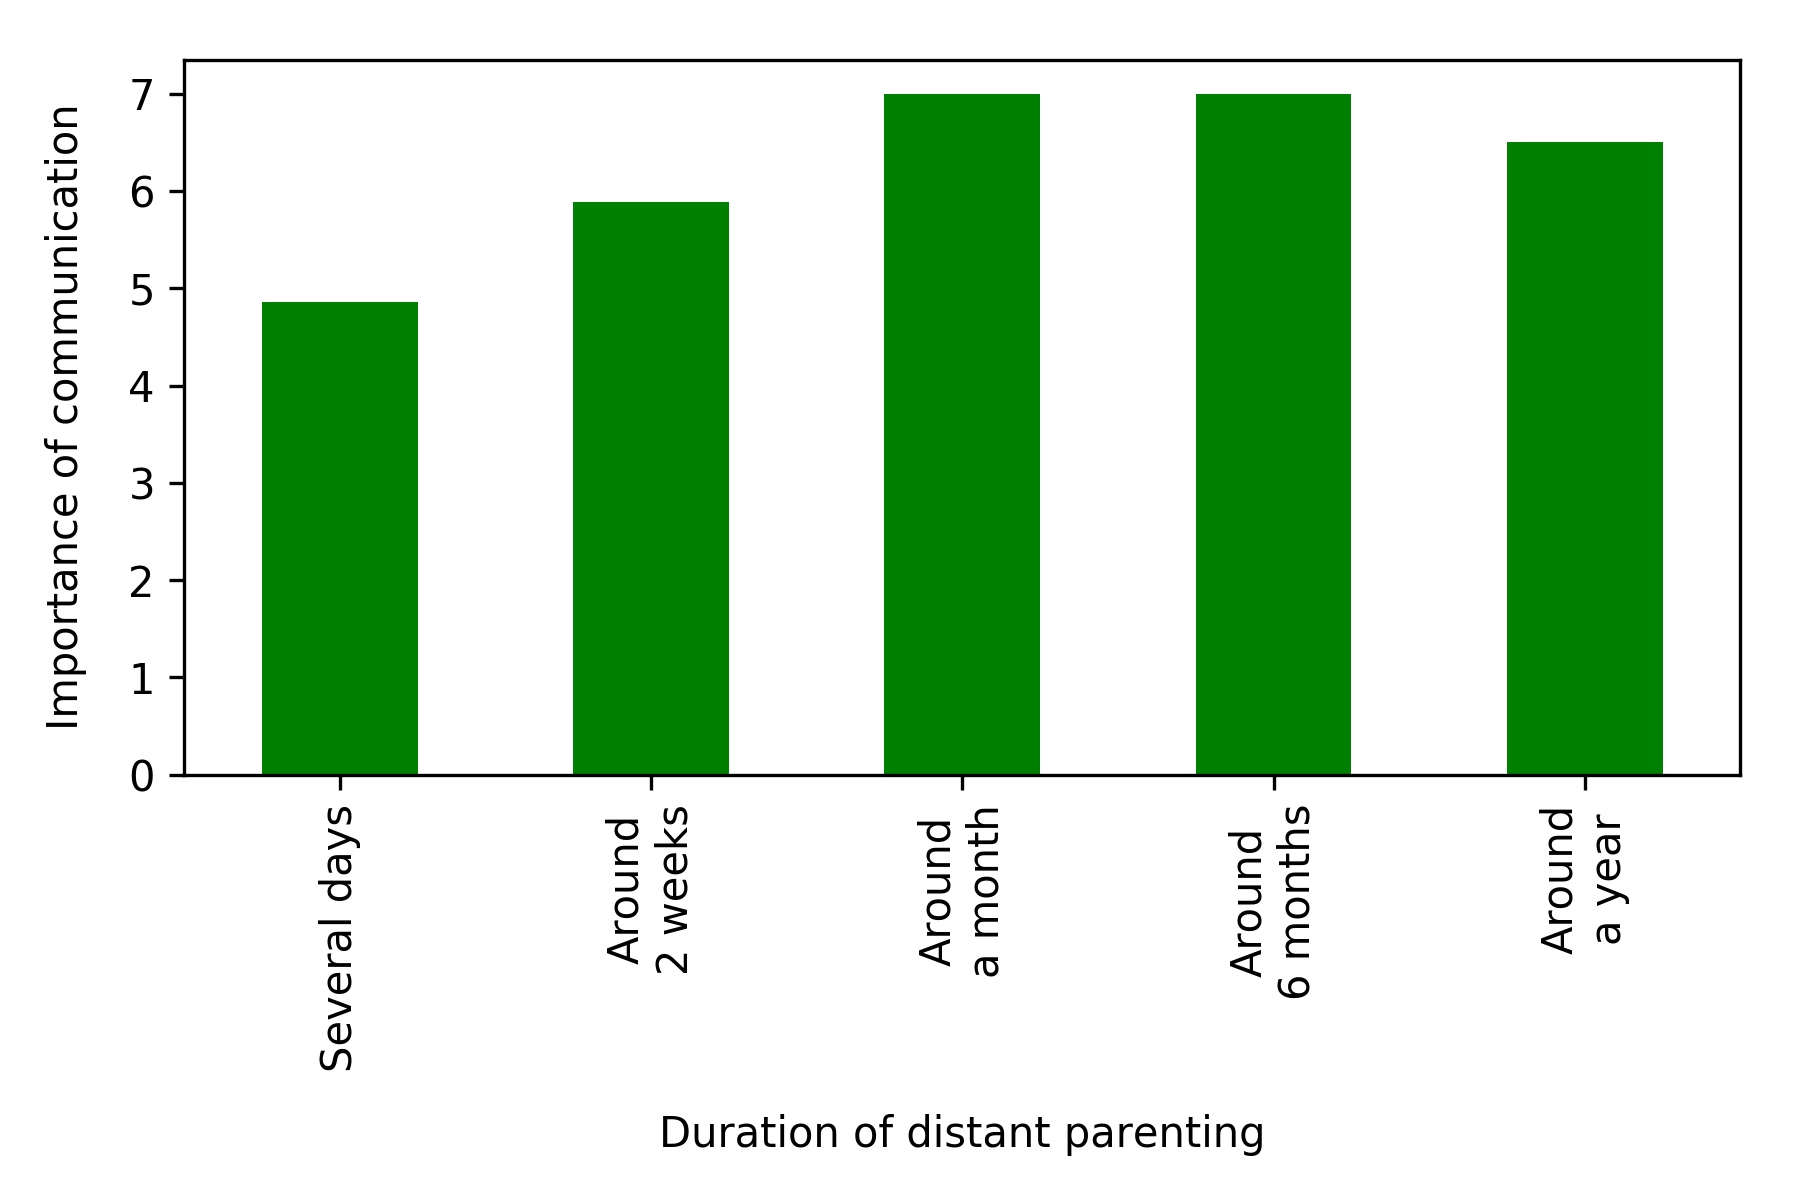
\includegraphics[scale=0.58]{plots/plot_5.png}
    \caption{Importance of communication from the parent point according to duration of distant-parenting experience}
    \label{fig:plot_5}
\end{figure}

\begin{figure}[h!]
    \centering
    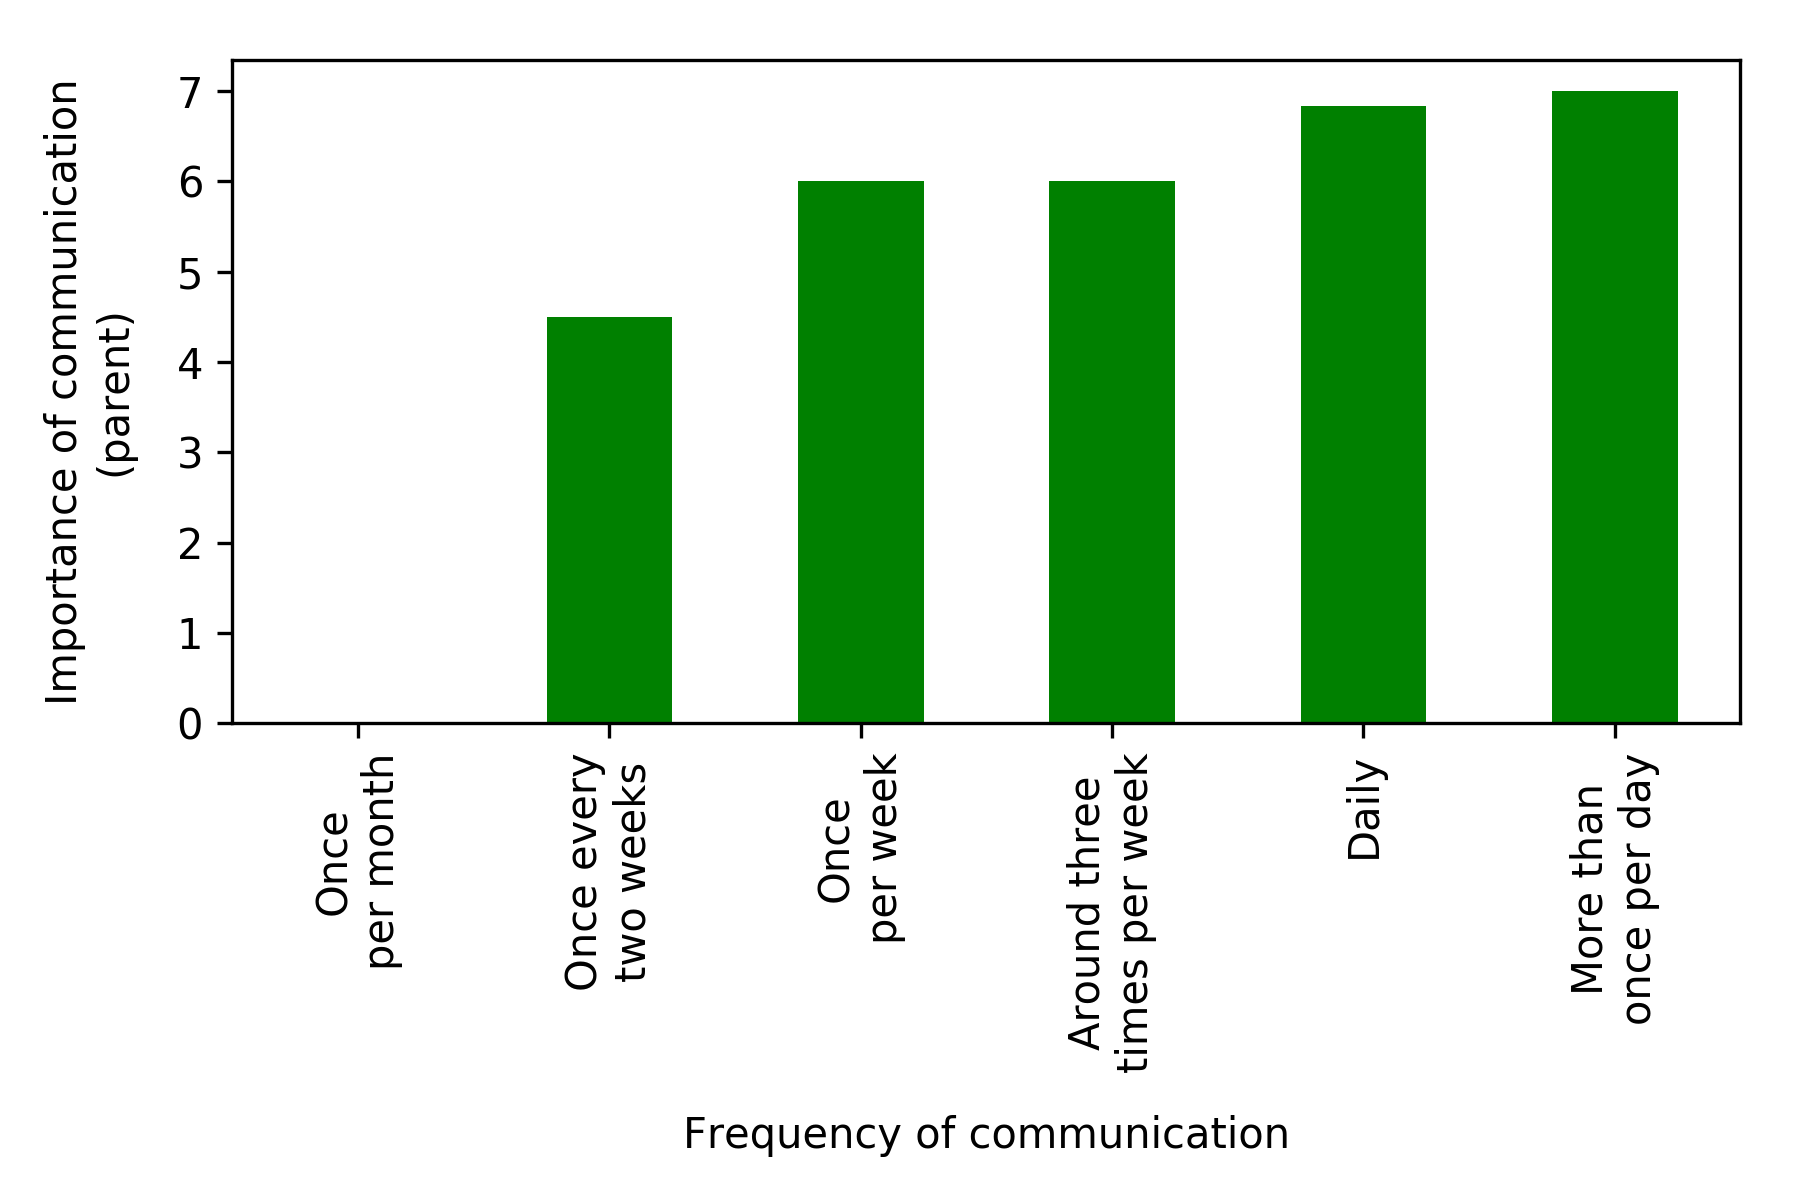
\includegraphics[scale=0.58]{plots/plot_8.png}
    \caption{Importance of communication from the parent point according to frequency of communication during distant-parenting experience}
    \label{fig:plot_8}
\end{figure}


\subsection{Interview protocol}
\label{appendix:interview_protocol}

The following interview protocol has been prepared for the research on “Communication Technologies for Left-Behind Children in Rural China”, in the scope of the “Global perspectives, local realities” SHS course. To continue our research on the Chinese field, by interviewing parents of left behind children, our assumptions could be tested and eventually further analyzed.

\vspace{4pt}
Please, fill in the missing informations as follows before starting the interview session:

Author: Matteo Yann Feo \& Simone Sanso

Session length: 40 minutes 

Participant Name: \hfill \_\_\_\_\_\_\_\_\_\_\_\_\_\_\_\_\_\_\_\_\_\_\_  $\leftarrow$ Fill in

Email: \hfill \_\_\_\_\_\_\_\_\_\_\_\_\_\_\_\_\_\_\_\_\_\_\_\_\_\_\_\_\_\_\_\_ $\leftarrow$ Fill in

Time/Date: \hfill \_\_\_\_\_\_\_\_\_\_\_\_\_\_\_\_\_\_\_\_\_\_\_\_\_\_\_\_ $\leftarrow$ Fill in

Location: \hfill \_\_\_\_\_\_\_\_\_\_\_\_\_\_\_\_\_\_\_\_\_\_\_\_\_\_\_\_\_ $\leftarrow$ Fill in

\vspace{6pt}
\subsubsection{Introduction \& Setup (5 mins)}

The session starts with a short introduction to what this interview is about, the context and the background for which it is being conducted. In the meantime, be sure that everything is setup correctly by double checking the following To-Do list:

\begin{todolist}
    \item Setup the recording tools and check if they work correctly.
    \item Prepare note-taking utilities, such as pen and paper.
    \item Verify the environment, being sure to have a relaxed location for the following 40 mins.
    \item In case a beverage is desired in the meantime, be sure to have it ready and available now.
    \item Be sure that your interviewed person has everything needed.
\end{todolist}

The introduction of the interview could be similar to the following one:

"Good morning and thank you for participating! I am Yann. I am studying at EPFL for a master degree in computer science. My main interest for this interview is to understand whether  a  technology  of  communication embedded in a smart toy could be helpful for parents distant from their children. During the interview, I will be having a conversation with you, asking questions that could help me to achieve my curiosity. In the meantime, my partner, will be assisting me by taking some notes. It is important to always remember that we are not evaluating you or your opinions in any way, there are no possible right and wrong answers that you could give. 
Here is how the session is going to proceed. Firstly, we'll break the ice by asking you a few general questions to know each other. We will record this interview, given your consent. We won't ever share this recording nor use it for anything else but pure support for this interview, so that I can go back and review things later to make sure we got everything right. Your name won't ever be linked to any result, so be relaxed and feel free to share your thoughts with us, without any troubles. Keep in mind that this is completely voluntary, the recording can be stopped whenever you want. Thus, if you don't like this idea, please let me know. 
How does all that sound to you? Do you have any questions at this point?"

\begin{todolist}
    \item Ask the interviewee to sign the written consent for recording purposes.
\end{todolist}

\vspace{2pt}
\subsubsection{Demographics \& Background (5 mins)}

This section will help us to create a background of the interviewee, while allowing him/her to start opening up to our questions. Use this session as a warming-up occasion to break the ice, while catching the first important features. Start to note down details on the interviewee, like gender, age, education level, marital status.

\begin{todolist}
    \item Tell us your name, and a little bit about yourself.
    \item Where do you come from?
    \item What is your occupation? Are you studying or working? In both cases, can you tell us something about it?
    \item Where are you currently living? Do you live with someone, or alone? 
\end{todolist}

\vspace{2pt}
\subsubsection{Main questions (20 mins)}

The following questions can be helpful to interpolate your impressions with the interviewee’s feelings and personal stories. Use them carefully as they might be intimidating for some people. Don’t forget to check for nonverbal behaviors, as they might be critical to have a complete idea of who you are interviewing, especially in this part. Note that the most important questions to be answered are marked with an asterisk (*).

\vspace{2pt}
(*) Pre-interview questions about their children :

\begin{todolist}
    \item How many children do you have?
    \item How old are they?
    \item What gender are they?
    \item Where do you they live?
    \item With who are they staying in your home village? (Lonely, with one of both parents, with grandparents or other relatives)
\end{todolist}

Main interview questions about the interviewed parent :

\begin{todolist}
    \item (*) How often and for how long do you come back home? 
    \item What is the main reason why you live far away from your children?
    \item How do you feel about this situation, not living with your children?
    \item Remember the last time you went back to your home village, how was the contact with your children? Was the meeting with your children as before you left them?
    \item During your childhood, have you ever experienced living far away from one of your parents? If yes, for how long? How did you live the situation? Could you tell us what was the main reason of your parent to out-migrate? How was the contact when meeting again with your parent? Could you communicate together, at that time, while being distant? (Check for non-verbal reactions while interviewee showcase personal experience)
    \item How common is your situation of distant parenting? Do you know any other persons in the same situation as you? How do they live it?
    \item (*) How would you define the importance of living with your children? In your case, is there a trade off between living with your children and having a job position? If yes, imagine that you could live in an ideal world, what would be the best solution? Would you rather work in your home village or be able to bring your children in town?
    \item (*) Do you own electronic devices? If yes, which ones? (Smartphone, computer, more…)
    \item (*) Do your children in your home village own electronic devices? If not, would they have the opportunity to use any? (Neighbourhood, school, etc.)
    \item (*) Do you use electronic devices to contact your children? If yes, how often? In general, are you calling your children when you have time? Or do they also get in touch with you, on their initiative?
    \item (*) From 0 to 7, how would you define the importance of communicating with your children? (0: insignificant, 4: neutral, 7: essential) (Check for non-verbal reactions while interviewee showcase personal experience)
\end{todolist}

\vspace{2pt}
\subsubsection{Interviewee's "show and tell" prototype (8 mins)}

This section is practical and allows us to showcase our project, related to the issue of distant parenting. In the context of CHIC (China Hardware Innovation Camp), a plush toy that encourages social interaction between parents and children, in a distant situation. It is a very resourceful moment, as it could bring additional and authentic feedback on a novel user scenario.

The explanation of the prototype could be similar to the following one:

"We have been working on this prototype. It is a plush toy that encourages social interaction, by having remotely turned on LEDs and sounds from a mobile application. Parents and children can therefore stay longer connected. Letting your children know when you think about them will help you stay 'toygether'\texttrademark."

Showcase the prototype and how it works with the mobile application.

\begin{todolist}
    \item What do you think about the idea?
    \item In your opinion, which are the positive and negative aspects?
    \item If you had the possibility to try this technology, would you be interested?
    \item What would you modify to improve it?
\end{todolist}

\vspace{2pt}
\subsubsection{Closing (2 mins)}

Thank the user at the end for participating to the session. Offer the possibility to ask any kind of question the interviewee might want to address you.  This is his/her time to wear the interviewer's shoes in your regards.

If the interviewee has no additional question, the interview is officially finished. Thank again your interviewee for the time and availability to participate to this session. Underline how useful his/her help has been for the project.
Turn off the recording tools only when you are completely sure that nothing will be added. It is important to not miss anything, so better have some extra recording to cut later.

Take some time to, directly after the end of the interview, write down some impressions you may have about the session. It is important to note down very early impressions about both verbal and physical languages, before they are forgotten. Those are the most authentic resources to get.




\subsection{List of contacts}
\label{appendix:contacts_list}
Below are listed all the contacts that have been reached, to spread as much as possible the survey.

\begin{itemize}
\item AFS programs for adolescents (15-18 years old): \\
Duration: 1 year \\
Kernstrasse 57, CH-8004 Zurich \\
Tel: +41 21 323 19 19 \\
Email: hello@afs.ch \\
https://www.afs.ch/fr/programmes-scolaires/ 

\vspace{4pt}
\item Canada-France exchange (16 years old): \\
Duration : 3 weeks \\
College of Jeanne d'Arc, 15 Rue du Chanoine Brun, 68100 Mulhouse, France \\
Tel: +33 3 89 45 36 31 \\
www.ejda.fr/ 

\vspace{4pt}
\item International exchange programs (14-18 years old): \\
Duration: 1 year \\
Rue Centrale 15, 1003 Lausanne \\
Tel: +41 800 822 811 \\
https://www.efswiss.ch/fr/highschool/ 

\vspace{4pt}
\item National observatory of the Erasmus + impact (1 year or 6 months): \\
Email: observatoire@agence-erasmus.fr \\
http://www.agence-erasmus.fr/page/observatoire/

\vspace{4pt}
\item Journal of international mobility:\\
Email: revue@agence-erasmus.fr \\
https://www.agence-erasmus.fr/page/JIM

\vspace{4pt}
\item Exchange program Brigitte Sauzay (14-17 years old): \\
Duration: 3 months in a host family in Germany and welcome 3 months in the family in France \\
https://www.ofaj.org/contact.html 

\vspace{4pt}
\item Internal exchanges and language stays in Switzerland (14-17 years old): \\
Duration: 1 year \\
College of Delémont, Avenue Station 7, 2800 Delémont \\
Tel: +41 32 421 00 70 \\
Email: info@coldel.org \\
http://www.college-delemont.ch/fr/Aide-aux-eleves/Echanges-et-sejours-linguistiques/Echanges-et-sejours-linguistiques.html \\
Cantonal manager of linguistic exchanges: \\
Patrice KAMBER, Pâquerettes 2, 2822 Courroux \\
- Prof: 032 435 65 92 / Private: 032 422 83 62 

\vspace{4pt}
\item Language Exchange and Mobility - DIP Geneva: \\
Catherine Fernandez Sonino: Head of Exchange \& Mobility DIP of the Cantonal Office for Language Exchange and Mobility \\
Chemin de l'Echo 5a, 1213 Onex \\
Email: catherine.fernandez@etat.ge.ch \\
Tel: +41 22 327 06 43, +41 79 175 56 46 \\
https://edu.ge.ch/site/elem/ 

\vspace{4pt}
\item Service of primary and secondary schools of Lausanne: \\
Place Chauderon 9, 5th floor, PO Box 5032, 1002 Lausanne \\
Tel: +41 21 315 64 11 - Fax: +41 21 315 60 04 \\
Email: seps@lausanne.ch \\
http://www.lausanne.ch/etablissements-scolaires/ 

\vspace{4pt}
\item Summer camp of Neuchatel:\\
Gisèle Nicaty \\
Quartier du Milieu 86, 2127 Les Bayards \\
Tel: +41 79 288 50 41, +41 32 866 17 29\\
Email: giroud.p-a@bluewin.ch\\
http://www.echanges-scolaires.com/index.php/fr/

\vspace{4pt}
\item Summer camp of the Grandes-Roches: \\
1348 le Brassus \\
Tel: +41 21 845 66 90 \\
Email: camps@asime.ch \\
http://www.grandesroches.ch/home 

\vspace{4pt}
\item Association of the Gros-de-Vaud Holiday Camp: \\
Mrs Florence Ethenoz \\
Chemin du Petit Record 60, 1040 Echallens \\
Tel: +41 21 881 10 76 \\
Email: info@colo-gros-de-vaud.ch \\
http://www.colo-gros-de-vaud.ch/clubdesk/www

\vspace{4pt}
\item Summer camp 4Fun: \\
Email: airfred@hotmail.com \\
http://4-fun.ch/ 

\vspace{4pt}
\item Summer camp CPV: \\
Swiss Village Street 14, PO Box 72, 1211 Geneva 8 \\
Tel: +41 22 809 49 79 \\
Email: info@camps.ch \\
http://www.camps.ch/fr/accueil 

\vspace{4pt}
\item Scouts of the Sacred Heart: \\
Jeanne Voruz \& Anne Thiébaud \\
Tel: +41 79 844 92 74 \& +41 79 284 50 38 \\
Email: cg@sacrescout.ch \\
http://www.sacrescout.ch/ 

\vspace{4pt}
\item Village Camps: \\
PO Box 1425, Rue de la Morache 14, 1260 Nyon 1 \\
Tel: +41 22 990 9400 \\
Email: camps@villagecamps.com \\
www.villagecamps.com

\vspace{4pt}
\item Alpadia Language Schools: \\
Grand-Rue 42, PO Box 1206, 1820 Montreux\\
Tel: +41 21 621 88 88\\
Email: info@alpadia.com\\
https://www.alpadia.com/fr/ 

\vspace{4pt}
\item Carol Panchaud Educom sàrl: \\
26 Route of Givrins, CH - 1276 Gingins\\
Tel: +41 22 776 69 15 \\
Email: carolpanchaud@educom.ch \\
http://educom.ch/fr

\vspace{4pt}
\item Caritas-Youth: \\
11, Jean-Violette Street, 1205 Geneva\\
Tel: +41 22 708 04 04\\
Email: info@caritas-jeunesse.ch\\
http://www.caritas-jeunesse.ch/

\vspace{4pt}
\item Holiday Camp St. Gervais: \\
CP 1337, 1211 Geneva 1\\
Tel: +41 78 896 71 84\\
Email: info@colonie-saint-gervais.ch\\
http://www.colonie-saint-gervais.ch/

\vspace{4pt}
\item Summer Camp of Ravoire - Camp Plein Soleil: \\
PO Box 87, CH-1920 Martigny 1\\
Email: info@camp-pleinsoleil.ch

\vspace{4pt}
\item Yverdon-les-Bains youth service and social cohesion: \\
Rue de Neuchâtel 2, 1400 Yverdon-les-Bains\\
Tel: +41 24 423 69 11\\
Email: vacances@yverdon-les-bains.ch\\
http://www.yverdon-les-bains.ch/prestations-deladministration/jeunesse-et-cohesion-sociale/enfanceetfamille/colonies-dete-et-dautomne/

\vspace{4pt}
\item fRilingue GmbH: \\
Stöckackerstrasse 93, 3018 Bern\\
Tel: +41 26 321 34 34 \\
Email: info@frilingue.com

\vspace{4pt}
\item Star Sports: \\
Path of Verger 2, PO Box 101, 1304 Cossonay-Ville\\
Tel: +41 79 356 44 61\\
Email: info@starsports.ch\\
http://www.starsports.ch/

\vspace{4pt}
\item Cap Loisirs Foundation: \\
34, Boulevard de Saint-Georges, 1205 Geneva\\
Tel: +41 22 731 86 00\\
Email: caploisirs@caploisirs.ch\\
http://www.caploisirs.ch/

\vspace{4pt}
\item SCE Holidays \& Events: \\
Rue de Lausanne 58, 1950 Sion\\
Tel: +41 79 693.33.64\\
Email: info@lescamps.ch\\
https://www.lescamps.ch/\\

\end{itemize}



% References of the Report
\thispagestyle{empty}
\vspace{1cm}
\begin{thebibliography}{9}
\addcontentsline{toc}{section}{References}

\bibitem{lab3-report} 
\textit{Lab 3.0 : Camera \& LCD conceptual design}. \\
CS-473 EPFL. Matteo Yann Feo \& Simone Aron Sanso. November 28th, 2017

\bibitem{lcd-controller} 
\textit{ILI9341 - a-Si TFT LCD Single Chip Driver 240RGBx320 Resolution and 262K color}. 
Rev. 1.11. ILI TECHNOLOGY CORP.

\bibitem{lcd-display} 
\textit{LT24 User Manual}. 
Altera. June 2015
 
\bibitem{avalon-interface} 
\textit{Avalon® Interface Specifications}.
MNL-AVABUSREF. Intel. May 2017.
 
\bibitem{fifo} 
\textit{Single- and Dual-Clock FIFO Megafunction}.
Rev. 4.0. Altera. May 2007.

\end{thebibliography}

\end{document}


% Appendix of the Report
\appendix

In the following appendix are presented the questions of the survey (... a list of figures and tables) to the reader.

\subsection{Questions of the survey}
\label{appendix:survey_questions}
In this section is shown how the participants were questioned towards the survey. Only the questions in English will be shown here, skipping the French translations.

\medskip \textit{Form about communication technologies :} \\
Realizing a research project about social sciences within EPFL University (Lausanne), we would like to understand the importance of communication between parents and children, when they are at a distance during a continuous period of time.

\vspace{4pt}
1. In what language would like to answer this form?

2. To contextualize, we seek either :

- parents of a child having spent a period of time away from the household,

- children, teenagers and young adults having spent a period of time away from their family.

After having read the description above, do you qualify yourself as a parent or a child?

\vspace{4pt}
\noindent - If "parent" was selected question 2: 

3.a. Are you the mother or the father?

4.a. Have you already been separated from your child for at least 3 days? (Exchange semester abroad, holidays, summer camp, boy-scout, etc.)

5.a. If there were more than one experience of distance parenting, please consider the earliest one of them through the rest of the form (when you were the youngest). What is the reason why your child was distant from you? 

6.a. For how long have you been distant from your child?

7.a. How old was your child at that time?

8.a. What is your child's gender?

9.a. How often did you use a communication technology with your distant child? (Text messages, phone calls, video chat, etc.)

10.a. What kind of information did you seek from communicating with your distant child?

11.a. How would you define the importance of being able to communicate with your distant child?

\vspace{4pt}
\noindent - If "child" was selected question 2: 

3.b. Have you already been separated from your family for at least 3 days? (Exchange semester abroad, holidays, summer camp, boy-scout, etc.)

3.b. If there were more than one experience of separation from your family, please consider the earliest one of them through the rest of the form (when you were the youngest). What is the reason why you were distant from your family? 

4.b. For how long have you been away?

5.b. How old were you at that time?

6.b. What is your gender?

7.b. How often did you use a communication technology with your family? (Text messages, phone calls, video chat, etc.)

8.b. What kind of information did you seek from communicating with your family?

9.b. How would you define the importance of being able to communicate with your family?


\subsection{Additional plots of the results}
\label{appendix:additional-plots}

The following plots have been computed for the analysis of the data collected via the survey on distant-parenting. This appendix contains a set of plots that didn't need particular attention during the discussion, but can still be source of investigation.

\begin{figure}[h!]
    \centering
    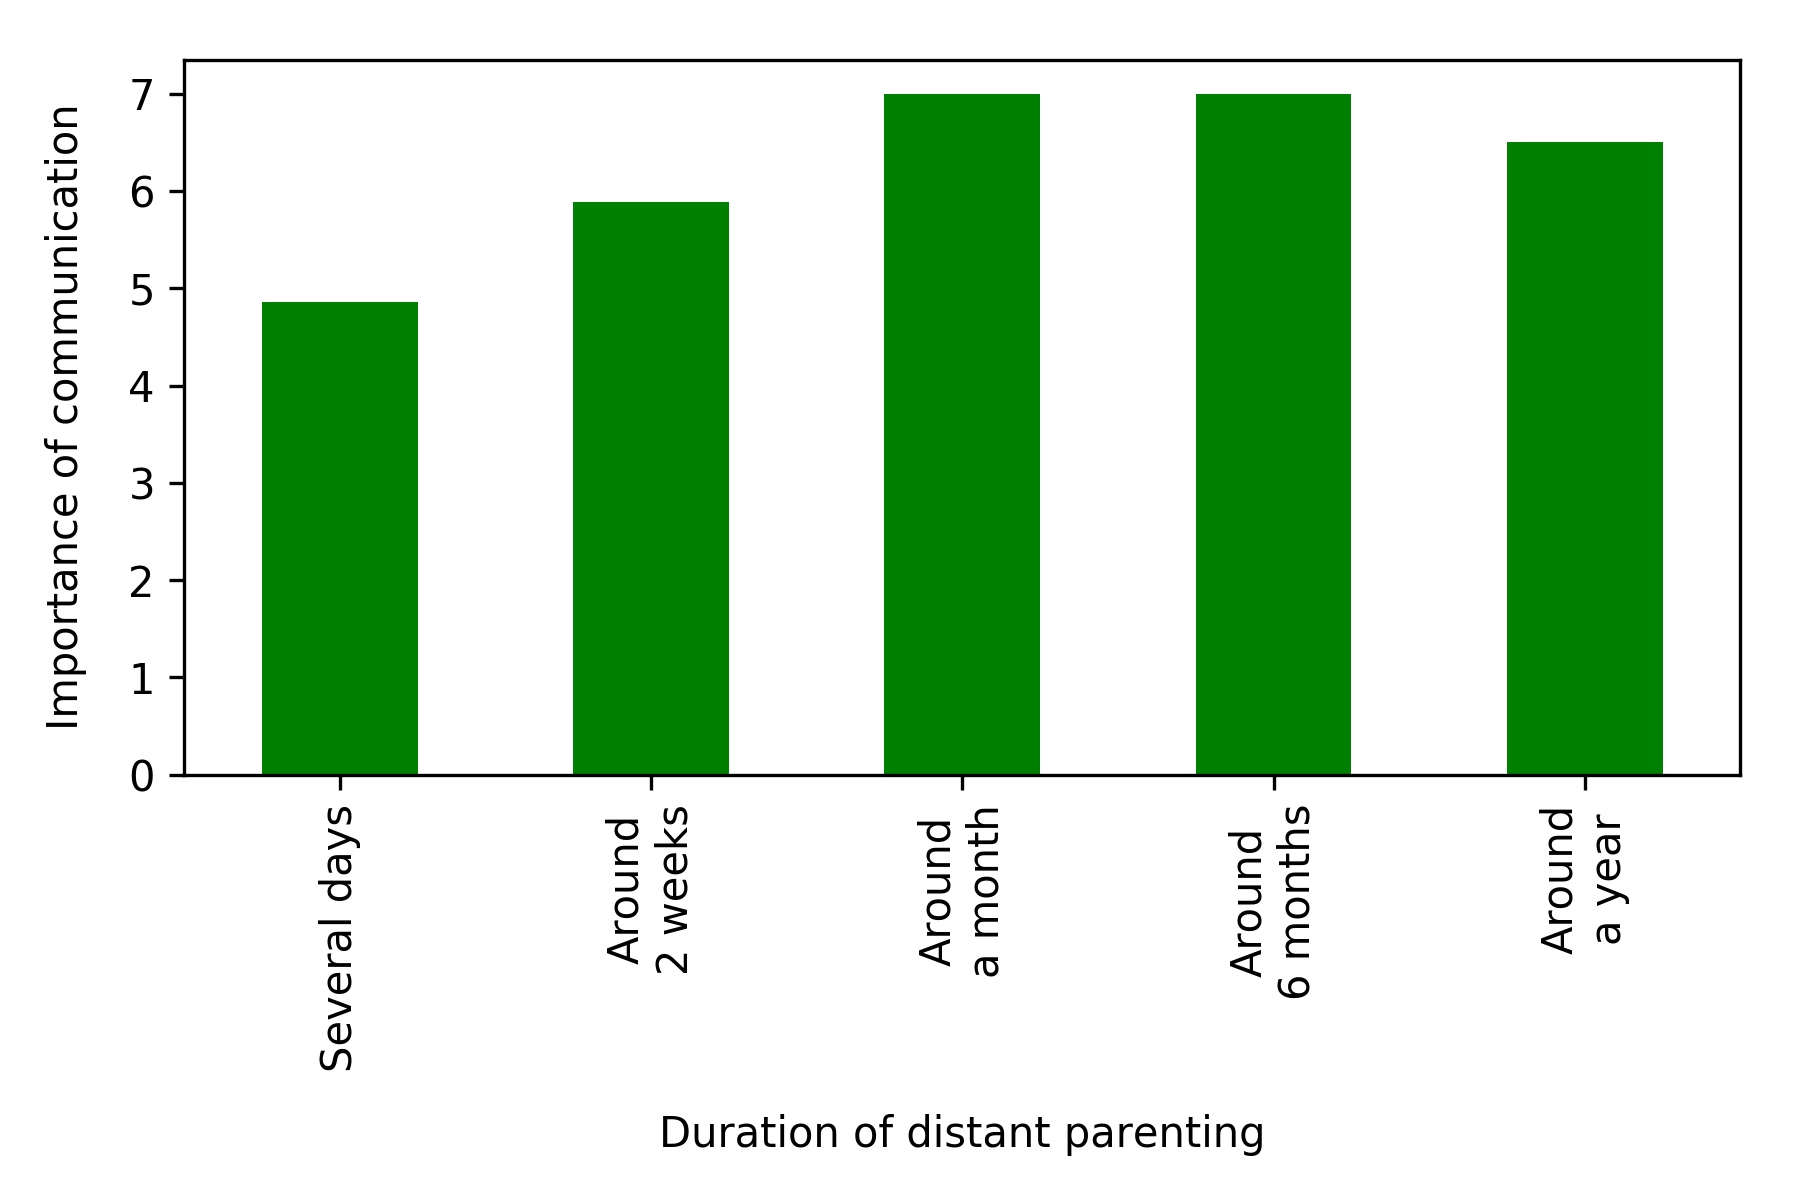
\includegraphics[scale=0.58]{plots/plot_5.png}
    \caption{Importance of communication from the parent point according to duration of distant-parenting experience}
    \label{fig:plot_5}
\end{figure}

\begin{figure}[h!]
    \centering
    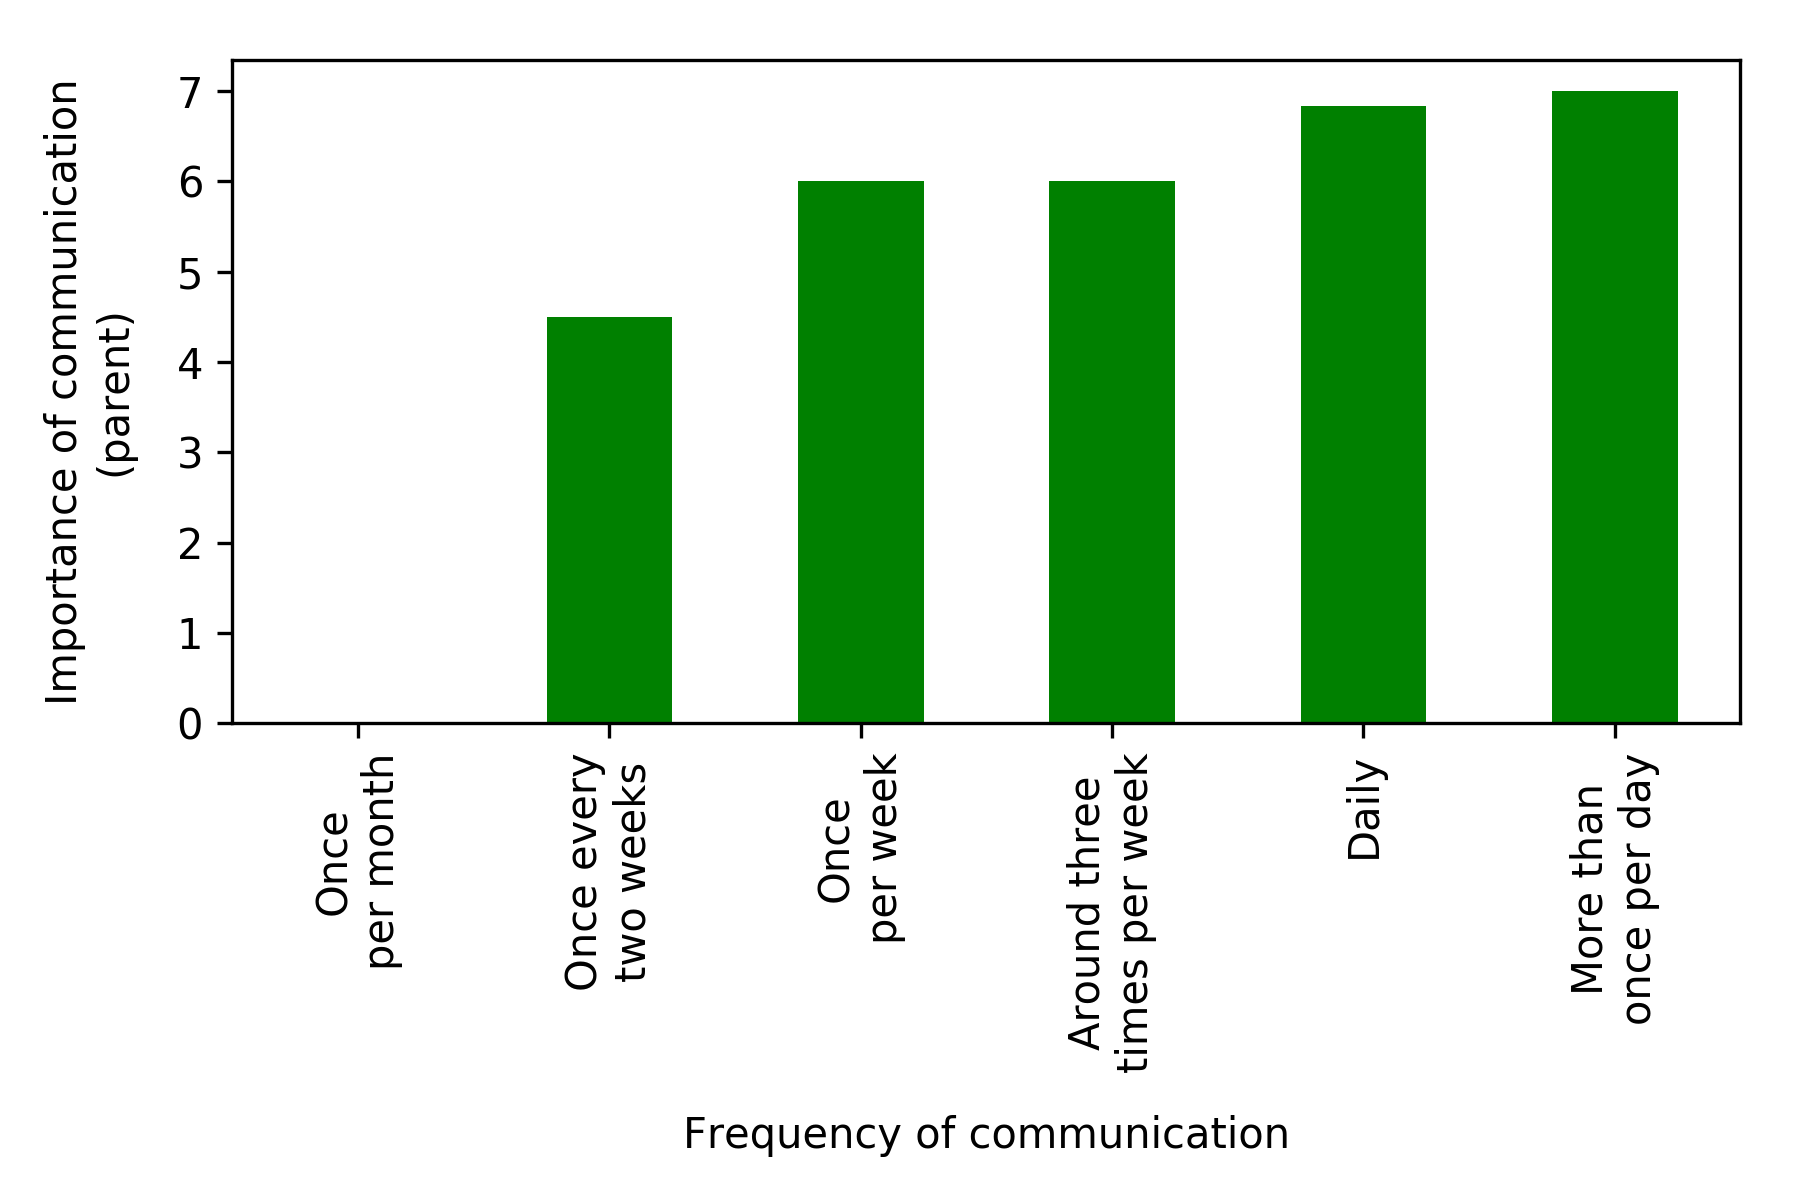
\includegraphics[scale=0.58]{plots/plot_8.png}
    \caption{Importance of communication from the parent point according to frequency of communication during distant-parenting experience}
    \label{fig:plot_8}
\end{figure}


\subsection{Interview protocol}
\label{appendix:interview_protocol}

The following interview protocol has been prepared for the research on “Communication Technologies for Left-Behind Children in Rural China”, in the scope of the “Global perspectives, local realities” SHS course. To continue our research on the Chinese field, by interviewing parents of left behind children, our assumptions could be tested and eventually further analyzed.

\vspace{4pt}
Please, fill in the missing informations as follows before starting the interview session:

Author: Matteo Yann Feo \& Simone Sanso

Session length: 40 minutes 

Participant Name: \hfill \_\_\_\_\_\_\_\_\_\_\_\_\_\_\_\_\_\_\_\_\_\_\_  $\leftarrow$ Fill in

Email: \hfill \_\_\_\_\_\_\_\_\_\_\_\_\_\_\_\_\_\_\_\_\_\_\_\_\_\_\_\_\_\_\_\_ $\leftarrow$ Fill in

Time/Date: \hfill \_\_\_\_\_\_\_\_\_\_\_\_\_\_\_\_\_\_\_\_\_\_\_\_\_\_\_\_ $\leftarrow$ Fill in

Location: \hfill \_\_\_\_\_\_\_\_\_\_\_\_\_\_\_\_\_\_\_\_\_\_\_\_\_\_\_\_\_ $\leftarrow$ Fill in

\vspace{6pt}
\subsubsection{Introduction \& Setup (5 mins)}

The session starts with a short introduction to what this interview is about, the context and the background for which it is being conducted. In the meantime, be sure that everything is setup correctly by double checking the following To-Do list:

\begin{todolist}
    \item Setup the recording tools and check if they work correctly.
    \item Prepare note-taking utilities, such as pen and paper.
    \item Verify the environment, being sure to have a relaxed location for the following 40 mins.
    \item In case a beverage is desired in the meantime, be sure to have it ready and available now.
    \item Be sure that your interviewed person has everything needed.
\end{todolist}

The introduction of the interview could be similar to the following one:

"Good morning and thank you for participating! I am Yann. I am studying at EPFL for a master degree in computer science. My main interest for this interview is to understand whether  a  technology  of  communication embedded in a smart toy could be helpful for parents distant from their children. During the interview, I will be having a conversation with you, asking questions that could help me to achieve my curiosity. In the meantime, my partner, will be assisting me by taking some notes. It is important to always remember that we are not evaluating you or your opinions in any way, there are no possible right and wrong answers that you could give. 
Here is how the session is going to proceed. Firstly, we'll break the ice by asking you a few general questions to know each other. We will record this interview, given your consent. We won't ever share this recording nor use it for anything else but pure support for this interview, so that I can go back and review things later to make sure we got everything right. Your name won't ever be linked to any result, so be relaxed and feel free to share your thoughts with us, without any troubles. Keep in mind that this is completely voluntary, the recording can be stopped whenever you want. Thus, if you don't like this idea, please let me know. 
How does all that sound to you? Do you have any questions at this point?"

\begin{todolist}
    \item Ask the interviewee to sign the written consent for recording purposes.
\end{todolist}

\vspace{2pt}
\subsubsection{Demographics \& Background (5 mins)}

This section will help us to create a background of the interviewee, while allowing him/her to start opening up to our questions. Use this session as a warming-up occasion to break the ice, while catching the first important features. Start to note down details on the interviewee, like gender, age, education level, marital status.

\begin{todolist}
    \item Tell us your name, and a little bit about yourself.
    \item Where do you come from?
    \item What is your occupation? Are you studying or working? In both cases, can you tell us something about it?
    \item Where are you currently living? Do you live with someone, or alone? 
\end{todolist}

\vspace{2pt}
\subsubsection{Main questions (20 mins)}

The following questions can be helpful to interpolate your impressions with the interviewee’s feelings and personal stories. Use them carefully as they might be intimidating for some people. Don’t forget to check for nonverbal behaviors, as they might be critical to have a complete idea of who you are interviewing, especially in this part. Note that the most important questions to be answered are marked with an asterisk (*).

\vspace{2pt}
(*) Pre-interview questions about their children :

\begin{todolist}
    \item How many children do you have?
    \item How old are they?
    \item What gender are they?
    \item Where do you they live?
    \item With who are they staying in your home village? (Lonely, with one of both parents, with grandparents or other relatives)
\end{todolist}

Main interview questions about the interviewed parent :

\begin{todolist}
    \item (*) How often and for how long do you come back home? 
    \item What is the main reason why you live far away from your children?
    \item How do you feel about this situation, not living with your children?
    \item Remember the last time you went back to your home village, how was the contact with your children? Was the meeting with your children as before you left them?
    \item During your childhood, have you ever experienced living far away from one of your parents? If yes, for how long? How did you live the situation? Could you tell us what was the main reason of your parent to out-migrate? How was the contact when meeting again with your parent? Could you communicate together, at that time, while being distant? (Check for non-verbal reactions while interviewee showcase personal experience)
    \item How common is your situation of distant parenting? Do you know any other persons in the same situation as you? How do they live it?
    \item (*) How would you define the importance of living with your children? In your case, is there a trade off between living with your children and having a job position? If yes, imagine that you could live in an ideal world, what would be the best solution? Would you rather work in your home village or be able to bring your children in town?
    \item (*) Do you own electronic devices? If yes, which ones? (Smartphone, computer, more…)
    \item (*) Do your children in your home village own electronic devices? If not, would they have the opportunity to use any? (Neighbourhood, school, etc.)
    \item (*) Do you use electronic devices to contact your children? If yes, how often? In general, are you calling your children when you have time? Or do they also get in touch with you, on their initiative?
    \item (*) From 0 to 7, how would you define the importance of communicating with your children? (0: insignificant, 4: neutral, 7: essential) (Check for non-verbal reactions while interviewee showcase personal experience)
\end{todolist}

\vspace{2pt}
\subsubsection{Interviewee's "show and tell" prototype (8 mins)}

This section is practical and allows us to showcase our project, related to the issue of distant parenting. In the context of CHIC (China Hardware Innovation Camp), a plush toy that encourages social interaction between parents and children, in a distant situation. It is a very resourceful moment, as it could bring additional and authentic feedback on a novel user scenario.

The explanation of the prototype could be similar to the following one:

"We have been working on this prototype. It is a plush toy that encourages social interaction, by having remotely turned on LEDs and sounds from a mobile application. Parents and children can therefore stay longer connected. Letting your children know when you think about them will help you stay 'toygether'\texttrademark."

Showcase the prototype and how it works with the mobile application.

\begin{todolist}
    \item What do you think about the idea?
    \item In your opinion, which are the positive and negative aspects?
    \item If you had the possibility to try this technology, would you be interested?
    \item What would you modify to improve it?
\end{todolist}

\vspace{2pt}
\subsubsection{Closing (2 mins)}

Thank the user at the end for participating to the session. Offer the possibility to ask any kind of question the interviewee might want to address you.  This is his/her time to wear the interviewer's shoes in your regards.

If the interviewee has no additional question, the interview is officially finished. Thank again your interviewee for the time and availability to participate to this session. Underline how useful his/her help has been for the project.
Turn off the recording tools only when you are completely sure that nothing will be added. It is important to not miss anything, so better have some extra recording to cut later.

Take some time to, directly after the end of the interview, write down some impressions you may have about the session. It is important to note down very early impressions about both verbal and physical languages, before they are forgotten. Those are the most authentic resources to get.




\subsection{List of contacts}
\label{appendix:contacts_list}
Below are listed all the contacts that have been reached, to spread as much as possible the survey.

\begin{itemize}
\item AFS programs for adolescents (15-18 years old): \\
Duration: 1 year \\
Kernstrasse 57, CH-8004 Zurich \\
Tel: +41 21 323 19 19 \\
Email: hello@afs.ch \\
https://www.afs.ch/fr/programmes-scolaires/ 

\vspace{4pt}
\item Canada-France exchange (16 years old): \\
Duration : 3 weeks \\
College of Jeanne d'Arc, 15 Rue du Chanoine Brun, 68100 Mulhouse, France \\
Tel: +33 3 89 45 36 31 \\
www.ejda.fr/ 

\vspace{4pt}
\item International exchange programs (14-18 years old): \\
Duration: 1 year \\
Rue Centrale 15, 1003 Lausanne \\
Tel: +41 800 822 811 \\
https://www.efswiss.ch/fr/highschool/ 

\vspace{4pt}
\item National observatory of the Erasmus + impact (1 year or 6 months): \\
Email: observatoire@agence-erasmus.fr \\
http://www.agence-erasmus.fr/page/observatoire/

\vspace{4pt}
\item Journal of international mobility:\\
Email: revue@agence-erasmus.fr \\
https://www.agence-erasmus.fr/page/JIM

\vspace{4pt}
\item Exchange program Brigitte Sauzay (14-17 years old): \\
Duration: 3 months in a host family in Germany and welcome 3 months in the family in France \\
https://www.ofaj.org/contact.html 

\vspace{4pt}
\item Internal exchanges and language stays in Switzerland (14-17 years old): \\
Duration: 1 year \\
College of Delémont, Avenue Station 7, 2800 Delémont \\
Tel: +41 32 421 00 70 \\
Email: info@coldel.org \\
http://www.college-delemont.ch/fr/Aide-aux-eleves/Echanges-et-sejours-linguistiques/Echanges-et-sejours-linguistiques.html \\
Cantonal manager of linguistic exchanges: \\
Patrice KAMBER, Pâquerettes 2, 2822 Courroux \\
- Prof: 032 435 65 92 / Private: 032 422 83 62 

\vspace{4pt}
\item Language Exchange and Mobility - DIP Geneva: \\
Catherine Fernandez Sonino: Head of Exchange \& Mobility DIP of the Cantonal Office for Language Exchange and Mobility \\
Chemin de l'Echo 5a, 1213 Onex \\
Email: catherine.fernandez@etat.ge.ch \\
Tel: +41 22 327 06 43, +41 79 175 56 46 \\
https://edu.ge.ch/site/elem/ 

\vspace{4pt}
\item Service of primary and secondary schools of Lausanne: \\
Place Chauderon 9, 5th floor, PO Box 5032, 1002 Lausanne \\
Tel: +41 21 315 64 11 - Fax: +41 21 315 60 04 \\
Email: seps@lausanne.ch \\
http://www.lausanne.ch/etablissements-scolaires/ 

\vspace{4pt}
\item Summer camp of Neuchatel:\\
Gisèle Nicaty \\
Quartier du Milieu 86, 2127 Les Bayards \\
Tel: +41 79 288 50 41, +41 32 866 17 29\\
Email: giroud.p-a@bluewin.ch\\
http://www.echanges-scolaires.com/index.php/fr/

\vspace{4pt}
\item Summer camp of the Grandes-Roches: \\
1348 le Brassus \\
Tel: +41 21 845 66 90 \\
Email: camps@asime.ch \\
http://www.grandesroches.ch/home 

\vspace{4pt}
\item Association of the Gros-de-Vaud Holiday Camp: \\
Mrs Florence Ethenoz \\
Chemin du Petit Record 60, 1040 Echallens \\
Tel: +41 21 881 10 76 \\
Email: info@colo-gros-de-vaud.ch \\
http://www.colo-gros-de-vaud.ch/clubdesk/www

\vspace{4pt}
\item Summer camp 4Fun: \\
Email: airfred@hotmail.com \\
http://4-fun.ch/ 

\vspace{4pt}
\item Summer camp CPV: \\
Swiss Village Street 14, PO Box 72, 1211 Geneva 8 \\
Tel: +41 22 809 49 79 \\
Email: info@camps.ch \\
http://www.camps.ch/fr/accueil 

\vspace{4pt}
\item Scouts of the Sacred Heart: \\
Jeanne Voruz \& Anne Thiébaud \\
Tel: +41 79 844 92 74 \& +41 79 284 50 38 \\
Email: cg@sacrescout.ch \\
http://www.sacrescout.ch/ 

\vspace{4pt}
\item Village Camps: \\
PO Box 1425, Rue de la Morache 14, 1260 Nyon 1 \\
Tel: +41 22 990 9400 \\
Email: camps@villagecamps.com \\
www.villagecamps.com

\vspace{4pt}
\item Alpadia Language Schools: \\
Grand-Rue 42, PO Box 1206, 1820 Montreux\\
Tel: +41 21 621 88 88\\
Email: info@alpadia.com\\
https://www.alpadia.com/fr/ 

\vspace{4pt}
\item Carol Panchaud Educom sàrl: \\
26 Route of Givrins, CH - 1276 Gingins\\
Tel: +41 22 776 69 15 \\
Email: carolpanchaud@educom.ch \\
http://educom.ch/fr

\vspace{4pt}
\item Caritas-Youth: \\
11, Jean-Violette Street, 1205 Geneva\\
Tel: +41 22 708 04 04\\
Email: info@caritas-jeunesse.ch\\
http://www.caritas-jeunesse.ch/

\vspace{4pt}
\item Holiday Camp St. Gervais: \\
CP 1337, 1211 Geneva 1\\
Tel: +41 78 896 71 84\\
Email: info@colonie-saint-gervais.ch\\
http://www.colonie-saint-gervais.ch/

\vspace{4pt}
\item Summer Camp of Ravoire - Camp Plein Soleil: \\
PO Box 87, CH-1920 Martigny 1\\
Email: info@camp-pleinsoleil.ch

\vspace{4pt}
\item Yverdon-les-Bains youth service and social cohesion: \\
Rue de Neuchâtel 2, 1400 Yverdon-les-Bains\\
Tel: +41 24 423 69 11\\
Email: vacances@yverdon-les-bains.ch\\
http://www.yverdon-les-bains.ch/prestations-deladministration/jeunesse-et-cohesion-sociale/enfanceetfamille/colonies-dete-et-dautomne/

\vspace{4pt}
\item fRilingue GmbH: \\
Stöckackerstrasse 93, 3018 Bern\\
Tel: +41 26 321 34 34 \\
Email: info@frilingue.com

\vspace{4pt}
\item Star Sports: \\
Path of Verger 2, PO Box 101, 1304 Cossonay-Ville\\
Tel: +41 79 356 44 61\\
Email: info@starsports.ch\\
http://www.starsports.ch/

\vspace{4pt}
\item Cap Loisirs Foundation: \\
34, Boulevard de Saint-Georges, 1205 Geneva\\
Tel: +41 22 731 86 00\\
Email: caploisirs@caploisirs.ch\\
http://www.caploisirs.ch/

\vspace{4pt}
\item SCE Holidays \& Events: \\
Rue de Lausanne 58, 1950 Sion\\
Tel: +41 79 693.33.64\\
Email: info@lescamps.ch\\
https://www.lescamps.ch/\\

\end{itemize}



% References of the Report
\thispagestyle{empty}
\vspace{1cm}
\begin{thebibliography}{9}
\addcontentsline{toc}{section}{References}

\bibitem{lab3-report} 
\textit{Lab 3.0 : Camera \& LCD conceptual design}. \\
CS-473 EPFL. Matteo Yann Feo \& Simone Aron Sanso. November 28th, 2017

\bibitem{lcd-controller} 
\textit{ILI9341 - a-Si TFT LCD Single Chip Driver 240RGBx320 Resolution and 262K color}. 
Rev. 1.11. ILI TECHNOLOGY CORP.

\bibitem{lcd-display} 
\textit{LT24 User Manual}. 
Altera. June 2015
 
\bibitem{avalon-interface} 
\textit{Avalon® Interface Specifications}.
MNL-AVABUSREF. Intel. May 2017.
 
\bibitem{fifo} 
\textit{Single- and Dual-Clock FIFO Megafunction}.
Rev. 4.0. Altera. May 2007.

\end{thebibliography}

\end{document}


\documentclass[a4paper,12pt]{article}

%% Layout
\usepackage[utf8]{inputenc}
\usepackage{palatino}
\usepackage[T1]{fontenc}
\usepackage[8pt]{extsizes}

\usepackage{geometry}
\geometry{
    a4paper,
    total={170mm,257mm},
    left=30mm,
    right=30mm,
    top=30mm,
    bottom=30mm,
 } 

%% Useful packages
\usepackage{amsmath}
\usepackage{amssymb}
\usepackage{mathtools}
\usepackage{microtype}

\usepackage[usenames, dvipsnames]{xcolor}
\usepackage{graphicx}
\usepackage{wrapfig}
\usepackage{subfig}
\usepackage{tabularx}
\usepackage{float}
\usepackage{caption}
\usepackage{multirow}
\usepackage{color, colortbl}
\usepackage{enumerate}

\usepackage{hyperref}
\usepackage{url}

\usepackage[english]{babel}
\usepackage{units}

\usepackage{textcomp}
\usepackage{titling}
\usepackage{blindtext}
\usepackage{listings}

\usepackage{braket}
\usepackage{rotating}

%\setlength{\droptitle}{-4em}     % Eliminate the default vertical space
%\addtolength{\droptitle}{-4pt}

\title{
    \centering
	
\includegraphics[width=0.5\textwidth]{images/Logo_EPFL.png}
    \\[1cm]
	\Huge China Hardware Innovation Camp\\[1cm]
    \huge Semester project report\\
    \rule{3.5cm}{0.9pt}\\[0.5cm]
    \huge HUM - 498 \vfill
    \normalsize
}

\author{
    \textbf{Laboratory group:}\\\\
    Chloe Dickson - \texttt{\href{mailto:chloe.dickson@epfl.ch}{simone.sanso@epfl.ch}} \\
    Matteo Yann Feo -    \texttt{\href{mailto:matteo.feo@epfl.ch}{matteo.feo@epfl.ch}} \\
    Simone Aron Sanso - \texttt{\href{mailto:simone.sanso@epfl.ch}{simone.sanso@epfl.ch}} \\\\
}

\date{\vfill \today}

\lstdefinestyle{Python}{
  language=Python,                % choose the language of the code
  numbers=left,                   % where to put the line-numbers
  stepnumber=1,                   % the step between two line-numbers.        
  numbersep=5pt,                  % how far the line-numbers are from the code
  backgroundcolor=\color{white},  % choose the background color. You must add \usepackage{color}
  showspaces=false,               % show spaces adding particular underscores
  showstringspaces=false,         % underline spaces within strings
  showtabs=false,                 % show tabs within strings adding particular underscores
  tabsize=2,                      % sets default tabsize to 2 spaces
  captionpos=b,                   % sets the caption-position to bottom
  breaklines=true,                % sets automatic line breaking
  breakatwhitespace=true,         % sets if automatic breaks should only happen at whitespace
  frame=single, 
  basicstyle=\ttfamily,
  keywordstyle=\color{Green}\bfseries,
  stringstyle=\color{red}\ttfamily,
  commentstyle=\color{OliveGreen}\ttfamily,
  %morecomment=[l][\color{magenta}]{\#}
}


\begin{document}
\maketitle
\thispagestyle{empty}

\newpage
\thispagestyle{empty}
\setcounter{page}{0}

\tableofcontents

\documentclass[a4paper,12pt]{article}

%% Layout
\usepackage[utf8]{inputenc}
\usepackage{palatino}
\usepackage[T1]{fontenc}
\usepackage[8pt]{extsizes}

\usepackage{geometry}
\geometry{
    a4paper,
    total={170mm,257mm},
    left=30mm,
    right=30mm,
    top=30mm,
    bottom=30mm,
 } 

%% Useful packages
\usepackage{amsmath}
\usepackage{amssymb}
\usepackage{mathtools}
\usepackage{microtype}

\usepackage[usenames, dvipsnames]{xcolor}
\usepackage{graphicx}
\usepackage{wrapfig}
\usepackage{subfig}
\usepackage{tabularx}
\usepackage{float}
\usepackage{caption}
\usepackage{multirow}
\usepackage{color, colortbl}
\usepackage{enumerate}

\usepackage{hyperref}
\usepackage{url}

\usepackage[english]{babel}
\usepackage{units}

\usepackage{textcomp}
\usepackage{titling}
\usepackage{blindtext}
\usepackage{listings}

\usepackage{braket}
\usepackage{rotating}

%\setlength{\droptitle}{-4em}     % Eliminate the default vertical space
%\addtolength{\droptitle}{-4pt}

\title{
    \centering
	
\includegraphics[width=0.5\textwidth]{images/Logo_EPFL.png}
    \\[1cm]
	\Huge China Hardware Innovation Camp\\[1cm]
    \huge Semester project report\\
    \rule{3.5cm}{0.9pt}\\[0.5cm]
    \huge HUM - 498 \vfill
    \normalsize
}

\author{
    \textbf{Laboratory group:}\\\\
    Chloe Dickson - \texttt{\href{mailto:chloe.dickson@epfl.ch}{simone.sanso@epfl.ch}} \\
    Matteo Yann Feo -    \texttt{\href{mailto:matteo.feo@epfl.ch}{matteo.feo@epfl.ch}} \\
    Simone Aron Sanso - \texttt{\href{mailto:simone.sanso@epfl.ch}{simone.sanso@epfl.ch}} \\\\
}

\date{\vfill \today}

\lstdefinestyle{Python}{
  language=Python,                % choose the language of the code
  numbers=left,                   % where to put the line-numbers
  stepnumber=1,                   % the step between two line-numbers.        
  numbersep=5pt,                  % how far the line-numbers are from the code
  backgroundcolor=\color{white},  % choose the background color. You must add \usepackage{color}
  showspaces=false,               % show spaces adding particular underscores
  showstringspaces=false,         % underline spaces within strings
  showtabs=false,                 % show tabs within strings adding particular underscores
  tabsize=2,                      % sets default tabsize to 2 spaces
  captionpos=b,                   % sets the caption-position to bottom
  breaklines=true,                % sets automatic line breaking
  breakatwhitespace=true,         % sets if automatic breaks should only happen at whitespace
  frame=single, 
  basicstyle=\ttfamily,
  keywordstyle=\color{Green}\bfseries,
  stringstyle=\color{red}\ttfamily,
  commentstyle=\color{OliveGreen}\ttfamily,
  %morecomment=[l][\color{magenta}]{\#}
}


\begin{document}
\maketitle
\thispagestyle{empty}

\newpage
\thispagestyle{empty}
\setcounter{page}{0}

\tableofcontents

\documentclass[a4paper,12pt]{article}

%% Layout
\usepackage[utf8]{inputenc}
\usepackage{palatino}
\usepackage[T1]{fontenc}
\usepackage[8pt]{extsizes}

\usepackage{geometry}
\geometry{
    a4paper,
    total={170mm,257mm},
    left=30mm,
    right=30mm,
    top=30mm,
    bottom=30mm,
 } 

%% Useful packages
\usepackage{amsmath}
\usepackage{amssymb}
\usepackage{mathtools}
\usepackage{microtype}

\usepackage[usenames, dvipsnames]{xcolor}
\usepackage{graphicx}
\usepackage{wrapfig}
\usepackage{subfig}
\usepackage{tabularx}
\usepackage{float}
\usepackage{caption}
\usepackage{multirow}
\usepackage{color, colortbl}
\usepackage{enumerate}

\usepackage{hyperref}
\usepackage{url}

\usepackage[english]{babel}
\usepackage{units}

\usepackage{textcomp}
\usepackage{titling}
\usepackage{blindtext}
\usepackage{listings}

\usepackage{braket}
\usepackage{rotating}

%\setlength{\droptitle}{-4em}     % Eliminate the default vertical space
%\addtolength{\droptitle}{-4pt}

\title{
    \centering
	
\includegraphics[width=0.5\textwidth]{images/Logo_EPFL.png}
    \\[1cm]
	\Huge China Hardware Innovation Camp\\[1cm]
    \huge Semester project report\\
    \rule{3.5cm}{0.9pt}\\[0.5cm]
    \huge HUM - 498 \vfill
    \normalsize
}

\author{
    \textbf{Laboratory group:}\\\\
    Chloe Dickson - \texttt{\href{mailto:chloe.dickson@epfl.ch}{simone.sanso@epfl.ch}} \\
    Matteo Yann Feo -    \texttt{\href{mailto:matteo.feo@epfl.ch}{matteo.feo@epfl.ch}} \\
    Simone Aron Sanso - \texttt{\href{mailto:simone.sanso@epfl.ch}{simone.sanso@epfl.ch}} \\\\
}

\date{\vfill \today}

\lstdefinestyle{Python}{
  language=Python,                % choose the language of the code
  numbers=left,                   % where to put the line-numbers
  stepnumber=1,                   % the step between two line-numbers.        
  numbersep=5pt,                  % how far the line-numbers are from the code
  backgroundcolor=\color{white},  % choose the background color. You must add \usepackage{color}
  showspaces=false,               % show spaces adding particular underscores
  showstringspaces=false,         % underline spaces within strings
  showtabs=false,                 % show tabs within strings adding particular underscores
  tabsize=2,                      % sets default tabsize to 2 spaces
  captionpos=b,                   % sets the caption-position to bottom
  breaklines=true,                % sets automatic line breaking
  breakatwhitespace=true,         % sets if automatic breaks should only happen at whitespace
  frame=single, 
  basicstyle=\ttfamily,
  keywordstyle=\color{Green}\bfseries,
  stringstyle=\color{red}\ttfamily,
  commentstyle=\color{OliveGreen}\ttfamily,
  %morecomment=[l][\color{magenta}]{\#}
}


\begin{document}
\maketitle
\thispagestyle{empty}

\newpage
\thispagestyle{empty}
\setcounter{page}{0}

\tableofcontents

\input{sections/1_introduction/main.tex}

\input{sections/2_structure/main.tex}
    \input{sections/2_structure/subsection_A.tex}
    \input{sections/2_structure/subsection_B.tex}
    \input{sections/2_structure/subsection_C.tex}
    
\input{sections/3_images_tables/main.tex}

\input{sections/4_code/main.tex}

\input{sections/5_conclusion/main.tex}

\input{appendix.tex}

\input{bibliography.tex}

\end{document}


\documentclass[a4paper,12pt]{article}

%% Layout
\usepackage[utf8]{inputenc}
\usepackage{palatino}
\usepackage[T1]{fontenc}
\usepackage[8pt]{extsizes}

\usepackage{geometry}
\geometry{
    a4paper,
    total={170mm,257mm},
    left=30mm,
    right=30mm,
    top=30mm,
    bottom=30mm,
 } 

%% Useful packages
\usepackage{amsmath}
\usepackage{amssymb}
\usepackage{mathtools}
\usepackage{microtype}

\usepackage[usenames, dvipsnames]{xcolor}
\usepackage{graphicx}
\usepackage{wrapfig}
\usepackage{subfig}
\usepackage{tabularx}
\usepackage{float}
\usepackage{caption}
\usepackage{multirow}
\usepackage{color, colortbl}
\usepackage{enumerate}

\usepackage{hyperref}
\usepackage{url}

\usepackage[english]{babel}
\usepackage{units}

\usepackage{textcomp}
\usepackage{titling}
\usepackage{blindtext}
\usepackage{listings}

\usepackage{braket}
\usepackage{rotating}

%\setlength{\droptitle}{-4em}     % Eliminate the default vertical space
%\addtolength{\droptitle}{-4pt}

\title{
    \centering
	
\includegraphics[width=0.5\textwidth]{images/Logo_EPFL.png}
    \\[1cm]
	\Huge China Hardware Innovation Camp\\[1cm]
    \huge Semester project report\\
    \rule{3.5cm}{0.9pt}\\[0.5cm]
    \huge HUM - 498 \vfill
    \normalsize
}

\author{
    \textbf{Laboratory group:}\\\\
    Chloe Dickson - \texttt{\href{mailto:chloe.dickson@epfl.ch}{simone.sanso@epfl.ch}} \\
    Matteo Yann Feo -    \texttt{\href{mailto:matteo.feo@epfl.ch}{matteo.feo@epfl.ch}} \\
    Simone Aron Sanso - \texttt{\href{mailto:simone.sanso@epfl.ch}{simone.sanso@epfl.ch}} \\\\
}

\date{\vfill \today}

\lstdefinestyle{Python}{
  language=Python,                % choose the language of the code
  numbers=left,                   % where to put the line-numbers
  stepnumber=1,                   % the step between two line-numbers.        
  numbersep=5pt,                  % how far the line-numbers are from the code
  backgroundcolor=\color{white},  % choose the background color. You must add \usepackage{color}
  showspaces=false,               % show spaces adding particular underscores
  showstringspaces=false,         % underline spaces within strings
  showtabs=false,                 % show tabs within strings adding particular underscores
  tabsize=2,                      % sets default tabsize to 2 spaces
  captionpos=b,                   % sets the caption-position to bottom
  breaklines=true,                % sets automatic line breaking
  breakatwhitespace=true,         % sets if automatic breaks should only happen at whitespace
  frame=single, 
  basicstyle=\ttfamily,
  keywordstyle=\color{Green}\bfseries,
  stringstyle=\color{red}\ttfamily,
  commentstyle=\color{OliveGreen}\ttfamily,
  %morecomment=[l][\color{magenta}]{\#}
}


\begin{document}
\maketitle
\thispagestyle{empty}

\newpage
\thispagestyle{empty}
\setcounter{page}{0}

\tableofcontents

\input{sections/1_introduction/main.tex}

\input{sections/2_structure/main.tex}
    \input{sections/2_structure/subsection_A.tex}
    \input{sections/2_structure/subsection_B.tex}
    \input{sections/2_structure/subsection_C.tex}
    
\input{sections/3_images_tables/main.tex}

\input{sections/4_code/main.tex}

\input{sections/5_conclusion/main.tex}

\input{appendix.tex}

\input{bibliography.tex}

\end{document}

    %\newpage
\subsection{Subsection A}
\label{subsec:A} 

This is the first subsection. I am saved into a file \textit{subsection\_A.tex} in the same folder as my main file. Pay attention to the format in the label tag in order to reference to the subsection elsewhere. The subsection is called in the main file of the whole document !

\medskip Nunc pulvinar, risus sed gravida pretium, eros tellus vehicula turpis, eget bibendum nisi dolor sed erat. Pellentesque sit amet orci sed ligula dictum cursus. Morbi gravida ligula sapien, non tristique orci semper id. Ut sollicitudin est ut nisi eleifend sollicitudin. Vivamus blandit congue risus id porttitor. Donec sed blandit mauris. Integer est leo, dapibus sed felis et, vulputate sagittis enim. Quisque eget purus vitae metus placerat rhoncus. Nulla eget lacus nec felis tincidunt suscipit ac eget tellus. Ut at augue fermentum, mattis justo sed, consectetur quam. Donec blandit euismod nisi ac auctor.
    %\newpage
\subsection{Subsection B}
\label{subsec:B} 

This is the second subsection. I am also saved into a file \textit{subsection\_B.tex} in the same folder as my main file. Pay attention to the format in the label tag in order to reference to the subsection elsewhere. The subsection is called in the main file of the whole document !

\medskip Nunc pulvinar, risus sed gravida pretium, eros tellus vehicula turpis, eget bibendum nisi dolor sed erat. Pellentesque sit amet orci sed ligula dictum cursus. Morbi gravida ligula sapien, non tristique orci semper id. Ut sollicitudin est ut nisi eleifend sollicitudin. Vivamus blandit congue risus id porttitor. Donec sed blandit mauris. Integer est leo, dapibus sed felis et, vulputate sagittis enim. Quisque eget purus vitae metus placerat rhoncus. Nulla eget lacus nec felis tincidunt suscipit ac eget tellus. Ut at augue fermentum, mattis justo sed, consectetur quam. Donec blandit euismod nisi ac auctor.
    %\newpage
\subsection{Subsection C}
\label{subsec:C} 

Okay, you got it by now ;-)
    
\documentclass[a4paper,12pt]{article}

%% Layout
\usepackage[utf8]{inputenc}
\usepackage{palatino}
\usepackage[T1]{fontenc}
\usepackage[8pt]{extsizes}

\usepackage{geometry}
\geometry{
    a4paper,
    total={170mm,257mm},
    left=30mm,
    right=30mm,
    top=30mm,
    bottom=30mm,
 } 

%% Useful packages
\usepackage{amsmath}
\usepackage{amssymb}
\usepackage{mathtools}
\usepackage{microtype}

\usepackage[usenames, dvipsnames]{xcolor}
\usepackage{graphicx}
\usepackage{wrapfig}
\usepackage{subfig}
\usepackage{tabularx}
\usepackage{float}
\usepackage{caption}
\usepackage{multirow}
\usepackage{color, colortbl}
\usepackage{enumerate}

\usepackage{hyperref}
\usepackage{url}

\usepackage[english]{babel}
\usepackage{units}

\usepackage{textcomp}
\usepackage{titling}
\usepackage{blindtext}
\usepackage{listings}

\usepackage{braket}
\usepackage{rotating}

%\setlength{\droptitle}{-4em}     % Eliminate the default vertical space
%\addtolength{\droptitle}{-4pt}

\title{
    \centering
	
\includegraphics[width=0.5\textwidth]{images/Logo_EPFL.png}
    \\[1cm]
	\Huge China Hardware Innovation Camp\\[1cm]
    \huge Semester project report\\
    \rule{3.5cm}{0.9pt}\\[0.5cm]
    \huge HUM - 498 \vfill
    \normalsize
}

\author{
    \textbf{Laboratory group:}\\\\
    Chloe Dickson - \texttt{\href{mailto:chloe.dickson@epfl.ch}{simone.sanso@epfl.ch}} \\
    Matteo Yann Feo -    \texttt{\href{mailto:matteo.feo@epfl.ch}{matteo.feo@epfl.ch}} \\
    Simone Aron Sanso - \texttt{\href{mailto:simone.sanso@epfl.ch}{simone.sanso@epfl.ch}} \\\\
}

\date{\vfill \today}

\lstdefinestyle{Python}{
  language=Python,                % choose the language of the code
  numbers=left,                   % where to put the line-numbers
  stepnumber=1,                   % the step between two line-numbers.        
  numbersep=5pt,                  % how far the line-numbers are from the code
  backgroundcolor=\color{white},  % choose the background color. You must add \usepackage{color}
  showspaces=false,               % show spaces adding particular underscores
  showstringspaces=false,         % underline spaces within strings
  showtabs=false,                 % show tabs within strings adding particular underscores
  tabsize=2,                      % sets default tabsize to 2 spaces
  captionpos=b,                   % sets the caption-position to bottom
  breaklines=true,                % sets automatic line breaking
  breakatwhitespace=true,         % sets if automatic breaks should only happen at whitespace
  frame=single, 
  basicstyle=\ttfamily,
  keywordstyle=\color{Green}\bfseries,
  stringstyle=\color{red}\ttfamily,
  commentstyle=\color{OliveGreen}\ttfamily,
  %morecomment=[l][\color{magenta}]{\#}
}


\begin{document}
\maketitle
\thispagestyle{empty}

\newpage
\thispagestyle{empty}
\setcounter{page}{0}

\tableofcontents

\input{sections/1_introduction/main.tex}

\input{sections/2_structure/main.tex}
    \input{sections/2_structure/subsection_A.tex}
    \input{sections/2_structure/subsection_B.tex}
    \input{sections/2_structure/subsection_C.tex}
    
\input{sections/3_images_tables/main.tex}

\input{sections/4_code/main.tex}

\input{sections/5_conclusion/main.tex}

\input{appendix.tex}

\input{bibliography.tex}

\end{document}


\documentclass[a4paper,12pt]{article}

%% Layout
\usepackage[utf8]{inputenc}
\usepackage{palatino}
\usepackage[T1]{fontenc}
\usepackage[8pt]{extsizes}

\usepackage{geometry}
\geometry{
    a4paper,
    total={170mm,257mm},
    left=30mm,
    right=30mm,
    top=30mm,
    bottom=30mm,
 } 

%% Useful packages
\usepackage{amsmath}
\usepackage{amssymb}
\usepackage{mathtools}
\usepackage{microtype}

\usepackage[usenames, dvipsnames]{xcolor}
\usepackage{graphicx}
\usepackage{wrapfig}
\usepackage{subfig}
\usepackage{tabularx}
\usepackage{float}
\usepackage{caption}
\usepackage{multirow}
\usepackage{color, colortbl}
\usepackage{enumerate}

\usepackage{hyperref}
\usepackage{url}

\usepackage[english]{babel}
\usepackage{units}

\usepackage{textcomp}
\usepackage{titling}
\usepackage{blindtext}
\usepackage{listings}

\usepackage{braket}
\usepackage{rotating}

%\setlength{\droptitle}{-4em}     % Eliminate the default vertical space
%\addtolength{\droptitle}{-4pt}

\title{
    \centering
	
\includegraphics[width=0.5\textwidth]{images/Logo_EPFL.png}
    \\[1cm]
	\Huge China Hardware Innovation Camp\\[1cm]
    \huge Semester project report\\
    \rule{3.5cm}{0.9pt}\\[0.5cm]
    \huge HUM - 498 \vfill
    \normalsize
}

\author{
    \textbf{Laboratory group:}\\\\
    Chloe Dickson - \texttt{\href{mailto:chloe.dickson@epfl.ch}{simone.sanso@epfl.ch}} \\
    Matteo Yann Feo -    \texttt{\href{mailto:matteo.feo@epfl.ch}{matteo.feo@epfl.ch}} \\
    Simone Aron Sanso - \texttt{\href{mailto:simone.sanso@epfl.ch}{simone.sanso@epfl.ch}} \\\\
}

\date{\vfill \today}

\lstdefinestyle{Python}{
  language=Python,                % choose the language of the code
  numbers=left,                   % where to put the line-numbers
  stepnumber=1,                   % the step between two line-numbers.        
  numbersep=5pt,                  % how far the line-numbers are from the code
  backgroundcolor=\color{white},  % choose the background color. You must add \usepackage{color}
  showspaces=false,               % show spaces adding particular underscores
  showstringspaces=false,         % underline spaces within strings
  showtabs=false,                 % show tabs within strings adding particular underscores
  tabsize=2,                      % sets default tabsize to 2 spaces
  captionpos=b,                   % sets the caption-position to bottom
  breaklines=true,                % sets automatic line breaking
  breakatwhitespace=true,         % sets if automatic breaks should only happen at whitespace
  frame=single, 
  basicstyle=\ttfamily,
  keywordstyle=\color{Green}\bfseries,
  stringstyle=\color{red}\ttfamily,
  commentstyle=\color{OliveGreen}\ttfamily,
  %morecomment=[l][\color{magenta}]{\#}
}


\begin{document}
\maketitle
\thispagestyle{empty}

\newpage
\thispagestyle{empty}
\setcounter{page}{0}

\tableofcontents

\input{sections/1_introduction/main.tex}

\input{sections/2_structure/main.tex}
    \input{sections/2_structure/subsection_A.tex}
    \input{sections/2_structure/subsection_B.tex}
    \input{sections/2_structure/subsection_C.tex}
    
\input{sections/3_images_tables/main.tex}

\input{sections/4_code/main.tex}

\input{sections/5_conclusion/main.tex}

\input{appendix.tex}

\input{bibliography.tex}

\end{document}


\documentclass[a4paper,12pt]{article}

%% Layout
\usepackage[utf8]{inputenc}
\usepackage{palatino}
\usepackage[T1]{fontenc}
\usepackage[8pt]{extsizes}

\usepackage{geometry}
\geometry{
    a4paper,
    total={170mm,257mm},
    left=30mm,
    right=30mm,
    top=30mm,
    bottom=30mm,
 } 

%% Useful packages
\usepackage{amsmath}
\usepackage{amssymb}
\usepackage{mathtools}
\usepackage{microtype}

\usepackage[usenames, dvipsnames]{xcolor}
\usepackage{graphicx}
\usepackage{wrapfig}
\usepackage{subfig}
\usepackage{tabularx}
\usepackage{float}
\usepackage{caption}
\usepackage{multirow}
\usepackage{color, colortbl}
\usepackage{enumerate}

\usepackage{hyperref}
\usepackage{url}

\usepackage[english]{babel}
\usepackage{units}

\usepackage{textcomp}
\usepackage{titling}
\usepackage{blindtext}
\usepackage{listings}

\usepackage{braket}
\usepackage{rotating}

%\setlength{\droptitle}{-4em}     % Eliminate the default vertical space
%\addtolength{\droptitle}{-4pt}

\title{
    \centering
	\includegraphics[width=0.5\textwidth]{images/Logo_EPFL.png}
    \\[1cm]
	\Huge China Hardware Innovation Camp\\[1cm]
    \huge Semester project report\\
    \rule{3.5cm}{0.9pt}\\[0.5cm]
    \huge HUM - 498 \vfill
    \normalsize
}

\author{
    \textbf{Laboratory group:}\\\\
    Chloe Dickson - \texttt{\href{mailto:chloe.dickson@epfl.ch}{simone.sanso@epfl.ch}} \\
    Matteo Yann Feo -    \texttt{\href{mailto:matteo.feo@epfl.ch}{matteo.feo@epfl.ch}} \\
    Simone Aron Sanso - \texttt{\href{mailto:simone.sanso@epfl.ch}{simone.sanso@epfl.ch}} \\\\
}

\date{\vfill \today}

\lstdefinestyle{Python}{
  language=Python,                % choose the language of the code
  numbers=left,                   % where to put the line-numbers
  stepnumber=1,                   % the step between two line-numbers.        
  numbersep=5pt,                  % how far the line-numbers are from the code
  backgroundcolor=\color{white},  % choose the background color. You must add \usepackage{color}
  showspaces=false,               % show spaces adding particular underscores
  showstringspaces=false,         % underline spaces within strings
  showtabs=false,                 % show tabs within strings adding particular underscores
  tabsize=2,                      % sets default tabsize to 2 spaces
  captionpos=b,                   % sets the caption-position to bottom
  breaklines=true,                % sets automatic line breaking
  breakatwhitespace=true,         % sets if automatic breaks should only happen at whitespace
  frame=single, 
  basicstyle=\ttfamily,
  keywordstyle=\color{Green}\bfseries,
  stringstyle=\color{red}\ttfamily,
  commentstyle=\color{OliveGreen}\ttfamily,
  %morecomment=[l][\color{magenta}]{\#}
}


\begin{document}
\maketitle
\thispagestyle{empty}

\newpage
\thispagestyle{empty}
\setcounter{page}{0}

\tableofcontents

\input{sections/1_introduction/main.tex}

\input{sections/2_structure/main.tex}
    \input{sections/2_structure/subsection_A.tex}
    \input{sections/2_structure/subsection_B.tex}
    \input{sections/2_structure/subsection_C.tex}
    
\input{sections/3_images_tables/main.tex}

\input{sections/4_code/main.tex}

\input{sections/5_conclusion/main.tex}

\input{appendix.tex}

\input{bibliography.tex}

\end{document}


% Appendix of the Report
\appendix

In the following appendix are presented the questions of the survey (... a list of figures and tables) to the reader.

\subsection{Questions of the survey}
\label{appendix:survey_questions}
In this section is shown how the participants were questioned towards the survey. Only the questions in English will be shown here, skipping the French translations.

\medskip \textit{Form about communication technologies :} \\
Realizing a research project about social sciences within EPFL University (Lausanne), we would like to understand the importance of communication between parents and children, when they are at a distance during a continuous period of time.

\vspace{4pt}
1. In what language would like to answer this form?

2. To contextualize, we seek either :

- parents of a child having spent a period of time away from the household,

- children, teenagers and young adults having spent a period of time away from their family.

After having read the description above, do you qualify yourself as a parent or a child?

\vspace{4pt}
\noindent - If "parent" was selected question 2: 

3.a. Are you the mother or the father?

4.a. Have you already been separated from your child for at least 3 days? (Exchange semester abroad, holidays, summer camp, boy-scout, etc.)

5.a. If there were more than one experience of distance parenting, please consider the earliest one of them through the rest of the form (when you were the youngest). What is the reason why your child was distant from you? 

6.a. For how long have you been distant from your child?

7.a. How old was your child at that time?

8.a. What is your child's gender?

9.a. How often did you use a communication technology with your distant child? (Text messages, phone calls, video chat, etc.)

10.a. What kind of information did you seek from communicating with your distant child?

11.a. How would you define the importance of being able to communicate with your distant child?

\vspace{4pt}
\noindent - If "child" was selected question 2: 

3.b. Have you already been separated from your family for at least 3 days? (Exchange semester abroad, holidays, summer camp, boy-scout, etc.)

3.b. If there were more than one experience of separation from your family, please consider the earliest one of them through the rest of the form (when you were the youngest). What is the reason why you were distant from your family? 

4.b. For how long have you been away?

5.b. How old were you at that time?

6.b. What is your gender?

7.b. How often did you use a communication technology with your family? (Text messages, phone calls, video chat, etc.)

8.b. What kind of information did you seek from communicating with your family?

9.b. How would you define the importance of being able to communicate with your family?


\subsection{Additional plots of the results}
\label{appendix:additional-plots}

The following plots have been computed for the analysis of the data collected via the survey on distant-parenting. This appendix contains a set of plots that didn't need particular attention during the discussion, but can still be source of investigation.

\begin{figure}[h!]
    \centering
    \includegraphics[scale=0.58]{plots/plot_5.png}
    \caption{Importance of communication from the parent point according to duration of distant-parenting experience}
    \label{fig:plot_5}
\end{figure}

\begin{figure}[h!]
    \centering
    \includegraphics[scale=0.58]{plots/plot_8.png}
    \caption{Importance of communication from the parent point according to frequency of communication during distant-parenting experience}
    \label{fig:plot_8}
\end{figure}


\subsection{Interview protocol}
\label{appendix:interview_protocol}

The following interview protocol has been prepared for the research on “Communication Technologies for Left-Behind Children in Rural China”, in the scope of the “Global perspectives, local realities” SHS course. To continue our research on the Chinese field, by interviewing parents of left behind children, our assumptions could be tested and eventually further analyzed.

\vspace{4pt}
Please, fill in the missing informations as follows before starting the interview session:

Author: Matteo Yann Feo \& Simone Sanso

Session length: 40 minutes 

Participant Name: \hfill \_\_\_\_\_\_\_\_\_\_\_\_\_\_\_\_\_\_\_\_\_\_\_  $\leftarrow$ Fill in

Email: \hfill \_\_\_\_\_\_\_\_\_\_\_\_\_\_\_\_\_\_\_\_\_\_\_\_\_\_\_\_\_\_\_\_ $\leftarrow$ Fill in

Time/Date: \hfill \_\_\_\_\_\_\_\_\_\_\_\_\_\_\_\_\_\_\_\_\_\_\_\_\_\_\_\_ $\leftarrow$ Fill in

Location: \hfill \_\_\_\_\_\_\_\_\_\_\_\_\_\_\_\_\_\_\_\_\_\_\_\_\_\_\_\_\_ $\leftarrow$ Fill in

\vspace{6pt}
\subsubsection{Introduction \& Setup (5 mins)}

The session starts with a short introduction to what this interview is about, the context and the background for which it is being conducted. In the meantime, be sure that everything is setup correctly by double checking the following To-Do list:

\begin{todolist}
    \item Setup the recording tools and check if they work correctly.
    \item Prepare note-taking utilities, such as pen and paper.
    \item Verify the environment, being sure to have a relaxed location for the following 40 mins.
    \item In case a beverage is desired in the meantime, be sure to have it ready and available now.
    \item Be sure that your interviewed person has everything needed.
\end{todolist}

The introduction of the interview could be similar to the following one:

"Good morning and thank you for participating! I am Yann. I am studying at EPFL for a master degree in computer science. My main interest for this interview is to understand whether  a  technology  of  communication embedded in a smart toy could be helpful for parents distant from their children. During the interview, I will be having a conversation with you, asking questions that could help me to achieve my curiosity. In the meantime, my partner, will be assisting me by taking some notes. It is important to always remember that we are not evaluating you or your opinions in any way, there are no possible right and wrong answers that you could give. 
Here is how the session is going to proceed. Firstly, we'll break the ice by asking you a few general questions to know each other. We will record this interview, given your consent. We won't ever share this recording nor use it for anything else but pure support for this interview, so that I can go back and review things later to make sure we got everything right. Your name won't ever be linked to any result, so be relaxed and feel free to share your thoughts with us, without any troubles. Keep in mind that this is completely voluntary, the recording can be stopped whenever you want. Thus, if you don't like this idea, please let me know. 
How does all that sound to you? Do you have any questions at this point?"

\begin{todolist}
    \item Ask the interviewee to sign the written consent for recording purposes.
\end{todolist}

\vspace{2pt}
\subsubsection{Demographics \& Background (5 mins)}

This section will help us to create a background of the interviewee, while allowing him/her to start opening up to our questions. Use this session as a warming-up occasion to break the ice, while catching the first important features. Start to note down details on the interviewee, like gender, age, education level, marital status.

\begin{todolist}
    \item Tell us your name, and a little bit about yourself.
    \item Where do you come from?
    \item What is your occupation? Are you studying or working? In both cases, can you tell us something about it?
    \item Where are you currently living? Do you live with someone, or alone? 
\end{todolist}

\vspace{2pt}
\subsubsection{Main questions (20 mins)}

The following questions can be helpful to interpolate your impressions with the interviewee’s feelings and personal stories. Use them carefully as they might be intimidating for some people. Don’t forget to check for nonverbal behaviors, as they might be critical to have a complete idea of who you are interviewing, especially in this part. Note that the most important questions to be answered are marked with an asterisk (*).

\vspace{2pt}
(*) Pre-interview questions about their children :

\begin{todolist}
    \item How many children do you have?
    \item How old are they?
    \item What gender are they?
    \item Where do you they live?
    \item With who are they staying in your home village? (Lonely, with one of both parents, with grandparents or other relatives)
\end{todolist}

Main interview questions about the interviewed parent :

\begin{todolist}
    \item (*) How often and for how long do you come back home? 
    \item What is the main reason why you live far away from your children?
    \item How do you feel about this situation, not living with your children?
    \item Remember the last time you went back to your home village, how was the contact with your children? Was the meeting with your children as before you left them?
    \item During your childhood, have you ever experienced living far away from one of your parents? If yes, for how long? How did you live the situation? Could you tell us what was the main reason of your parent to out-migrate? How was the contact when meeting again with your parent? Could you communicate together, at that time, while being distant? (Check for non-verbal reactions while interviewee showcase personal experience)
    \item How common is your situation of distant parenting? Do you know any other persons in the same situation as you? How do they live it?
    \item (*) How would you define the importance of living with your children? In your case, is there a trade off between living with your children and having a job position? If yes, imagine that you could live in an ideal world, what would be the best solution? Would you rather work in your home village or be able to bring your children in town?
    \item (*) Do you own electronic devices? If yes, which ones? (Smartphone, computer, more…)
    \item (*) Do your children in your home village own electronic devices? If not, would they have the opportunity to use any? (Neighbourhood, school, etc.)
    \item (*) Do you use electronic devices to contact your children? If yes, how often? In general, are you calling your children when you have time? Or do they also get in touch with you, on their initiative?
    \item (*) From 0 to 7, how would you define the importance of communicating with your children? (0: insignificant, 4: neutral, 7: essential) (Check for non-verbal reactions while interviewee showcase personal experience)
\end{todolist}

\vspace{2pt}
\subsubsection{Interviewee's "show and tell" prototype (8 mins)}

This section is practical and allows us to showcase our project, related to the issue of distant parenting. In the context of CHIC (China Hardware Innovation Camp), a plush toy that encourages social interaction between parents and children, in a distant situation. It is a very resourceful moment, as it could bring additional and authentic feedback on a novel user scenario.

The explanation of the prototype could be similar to the following one:

"We have been working on this prototype. It is a plush toy that encourages social interaction, by having remotely turned on LEDs and sounds from a mobile application. Parents and children can therefore stay longer connected. Letting your children know when you think about them will help you stay 'toygether'\texttrademark."

Showcase the prototype and how it works with the mobile application.

\begin{todolist}
    \item What do you think about the idea?
    \item In your opinion, which are the positive and negative aspects?
    \item If you had the possibility to try this technology, would you be interested?
    \item What would you modify to improve it?
\end{todolist}

\vspace{2pt}
\subsubsection{Closing (2 mins)}

Thank the user at the end for participating to the session. Offer the possibility to ask any kind of question the interviewee might want to address you.  This is his/her time to wear the interviewer's shoes in your regards.

If the interviewee has no additional question, the interview is officially finished. Thank again your interviewee for the time and availability to participate to this session. Underline how useful his/her help has been for the project.
Turn off the recording tools only when you are completely sure that nothing will be added. It is important to not miss anything, so better have some extra recording to cut later.

Take some time to, directly after the end of the interview, write down some impressions you may have about the session. It is important to note down very early impressions about both verbal and physical languages, before they are forgotten. Those are the most authentic resources to get.




\subsection{List of contacts}
\label{appendix:contacts_list}
Below are listed all the contacts that have been reached, to spread as much as possible the survey.

\begin{itemize}
\item AFS programs for adolescents (15-18 years old): \\
Duration: 1 year \\
Kernstrasse 57, CH-8004 Zurich \\
Tel: +41 21 323 19 19 \\
Email: hello@afs.ch \\
https://www.afs.ch/fr/programmes-scolaires/ 

\vspace{4pt}
\item Canada-France exchange (16 years old): \\
Duration : 3 weeks \\
College of Jeanne d'Arc, 15 Rue du Chanoine Brun, 68100 Mulhouse, France \\
Tel: +33 3 89 45 36 31 \\
www.ejda.fr/ 

\vspace{4pt}
\item International exchange programs (14-18 years old): \\
Duration: 1 year \\
Rue Centrale 15, 1003 Lausanne \\
Tel: +41 800 822 811 \\
https://www.efswiss.ch/fr/highschool/ 

\vspace{4pt}
\item National observatory of the Erasmus + impact (1 year or 6 months): \\
Email: observatoire@agence-erasmus.fr \\
http://www.agence-erasmus.fr/page/observatoire/

\vspace{4pt}
\item Journal of international mobility:\\
Email: revue@agence-erasmus.fr \\
https://www.agence-erasmus.fr/page/JIM

\vspace{4pt}
\item Exchange program Brigitte Sauzay (14-17 years old): \\
Duration: 3 months in a host family in Germany and welcome 3 months in the family in France \\
https://www.ofaj.org/contact.html 

\vspace{4pt}
\item Internal exchanges and language stays in Switzerland (14-17 years old): \\
Duration: 1 year \\
College of Delémont, Avenue Station 7, 2800 Delémont \\
Tel: +41 32 421 00 70 \\
Email: info@coldel.org \\
http://www.college-delemont.ch/fr/Aide-aux-eleves/Echanges-et-sejours-linguistiques/Echanges-et-sejours-linguistiques.html \\
Cantonal manager of linguistic exchanges: \\
Patrice KAMBER, Pâquerettes 2, 2822 Courroux \\
- Prof: 032 435 65 92 / Private: 032 422 83 62 

\vspace{4pt}
\item Language Exchange and Mobility - DIP Geneva: \\
Catherine Fernandez Sonino: Head of Exchange \& Mobility DIP of the Cantonal Office for Language Exchange and Mobility \\
Chemin de l'Echo 5a, 1213 Onex \\
Email: catherine.fernandez@etat.ge.ch \\
Tel: +41 22 327 06 43, +41 79 175 56 46 \\
https://edu.ge.ch/site/elem/ 

\vspace{4pt}
\item Service of primary and secondary schools of Lausanne: \\
Place Chauderon 9, 5th floor, PO Box 5032, 1002 Lausanne \\
Tel: +41 21 315 64 11 - Fax: +41 21 315 60 04 \\
Email: seps@lausanne.ch \\
http://www.lausanne.ch/etablissements-scolaires/ 

\vspace{4pt}
\item Summer camp of Neuchatel:\\
Gisèle Nicaty \\
Quartier du Milieu 86, 2127 Les Bayards \\
Tel: +41 79 288 50 41, +41 32 866 17 29\\
Email: giroud.p-a@bluewin.ch\\
http://www.echanges-scolaires.com/index.php/fr/

\vspace{4pt}
\item Summer camp of the Grandes-Roches: \\
1348 le Brassus \\
Tel: +41 21 845 66 90 \\
Email: camps@asime.ch \\
http://www.grandesroches.ch/home 

\vspace{4pt}
\item Association of the Gros-de-Vaud Holiday Camp: \\
Mrs Florence Ethenoz \\
Chemin du Petit Record 60, 1040 Echallens \\
Tel: +41 21 881 10 76 \\
Email: info@colo-gros-de-vaud.ch \\
http://www.colo-gros-de-vaud.ch/clubdesk/www

\vspace{4pt}
\item Summer camp 4Fun: \\
Email: airfred@hotmail.com \\
http://4-fun.ch/ 

\vspace{4pt}
\item Summer camp CPV: \\
Swiss Village Street 14, PO Box 72, 1211 Geneva 8 \\
Tel: +41 22 809 49 79 \\
Email: info@camps.ch \\
http://www.camps.ch/fr/accueil 

\vspace{4pt}
\item Scouts of the Sacred Heart: \\
Jeanne Voruz \& Anne Thiébaud \\
Tel: +41 79 844 92 74 \& +41 79 284 50 38 \\
Email: cg@sacrescout.ch \\
http://www.sacrescout.ch/ 

\vspace{4pt}
\item Village Camps: \\
PO Box 1425, Rue de la Morache 14, 1260 Nyon 1 \\
Tel: +41 22 990 9400 \\
Email: camps@villagecamps.com \\
www.villagecamps.com

\vspace{4pt}
\item Alpadia Language Schools: \\
Grand-Rue 42, PO Box 1206, 1820 Montreux\\
Tel: +41 21 621 88 88\\
Email: info@alpadia.com\\
https://www.alpadia.com/fr/ 

\vspace{4pt}
\item Carol Panchaud Educom sàrl: \\
26 Route of Givrins, CH - 1276 Gingins\\
Tel: +41 22 776 69 15 \\
Email: carolpanchaud@educom.ch \\
http://educom.ch/fr

\vspace{4pt}
\item Caritas-Youth: \\
11, Jean-Violette Street, 1205 Geneva\\
Tel: +41 22 708 04 04\\
Email: info@caritas-jeunesse.ch\\
http://www.caritas-jeunesse.ch/

\vspace{4pt}
\item Holiday Camp St. Gervais: \\
CP 1337, 1211 Geneva 1\\
Tel: +41 78 896 71 84\\
Email: info@colonie-saint-gervais.ch\\
http://www.colonie-saint-gervais.ch/

\vspace{4pt}
\item Summer Camp of Ravoire - Camp Plein Soleil: \\
PO Box 87, CH-1920 Martigny 1\\
Email: info@camp-pleinsoleil.ch

\vspace{4pt}
\item Yverdon-les-Bains youth service and social cohesion: \\
Rue de Neuchâtel 2, 1400 Yverdon-les-Bains\\
Tel: +41 24 423 69 11\\
Email: vacances@yverdon-les-bains.ch\\
http://www.yverdon-les-bains.ch/prestations-deladministration/jeunesse-et-cohesion-sociale/enfanceetfamille/colonies-dete-et-dautomne/

\vspace{4pt}
\item fRilingue GmbH: \\
Stöckackerstrasse 93, 3018 Bern\\
Tel: +41 26 321 34 34 \\
Email: info@frilingue.com

\vspace{4pt}
\item Star Sports: \\
Path of Verger 2, PO Box 101, 1304 Cossonay-Ville\\
Tel: +41 79 356 44 61\\
Email: info@starsports.ch\\
http://www.starsports.ch/

\vspace{4pt}
\item Cap Loisirs Foundation: \\
34, Boulevard de Saint-Georges, 1205 Geneva\\
Tel: +41 22 731 86 00\\
Email: caploisirs@caploisirs.ch\\
http://www.caploisirs.ch/

\vspace{4pt}
\item SCE Holidays \& Events: \\
Rue de Lausanne 58, 1950 Sion\\
Tel: +41 79 693.33.64\\
Email: info@lescamps.ch\\
https://www.lescamps.ch/\\

\end{itemize}



% References of the Report
\thispagestyle{empty}
\vspace{1cm}
\begin{thebibliography}{9}
\addcontentsline{toc}{section}{References}

\bibitem{lab3-report} 
\textit{Lab 3.0 : Camera \& LCD conceptual design}. \\
CS-473 EPFL. Matteo Yann Feo \& Simone Aron Sanso. November 28th, 2017

\bibitem{lcd-controller} 
\textit{ILI9341 - a-Si TFT LCD Single Chip Driver 240RGBx320 Resolution and 262K color}. 
Rev. 1.11. ILI TECHNOLOGY CORP.

\bibitem{lcd-display} 
\textit{LT24 User Manual}. 
Altera. June 2015
 
\bibitem{avalon-interface} 
\textit{Avalon® Interface Specifications}.
MNL-AVABUSREF. Intel. May 2017.
 
\bibitem{fifo} 
\textit{Single- and Dual-Clock FIFO Megafunction}.
Rev. 4.0. Altera. May 2007.

\end{thebibliography}

\end{document}


\documentclass[a4paper,12pt]{article}

%% Layout
\usepackage[utf8]{inputenc}
\usepackage{palatino}
\usepackage[T1]{fontenc}
\usepackage[8pt]{extsizes}

\usepackage{geometry}
\geometry{
    a4paper,
    total={170mm,257mm},
    left=30mm,
    right=30mm,
    top=30mm,
    bottom=30mm,
 } 

%% Useful packages
\usepackage{amsmath}
\usepackage{amssymb}
\usepackage{mathtools}
\usepackage{microtype}

\usepackage[usenames, dvipsnames]{xcolor}
\usepackage{graphicx}
\usepackage{wrapfig}
\usepackage{subfig}
\usepackage{tabularx}
\usepackage{float}
\usepackage{caption}
\usepackage{multirow}
\usepackage{color, colortbl}
\usepackage{enumerate}

\usepackage{hyperref}
\usepackage{url}

\usepackage[english]{babel}
\usepackage{units}

\usepackage{textcomp}
\usepackage{titling}
\usepackage{blindtext}
\usepackage{listings}

\usepackage{braket}
\usepackage{rotating}

%\setlength{\droptitle}{-4em}     % Eliminate the default vertical space
%\addtolength{\droptitle}{-4pt}

\title{
    \centering
	\includegraphics[width=0.5\textwidth]{images/Logo_EPFL.png}
    \\[1cm]
	\Huge China Hardware Innovation Camp\\[1cm]
    \huge Semester project report\\
    \rule{3.5cm}{0.9pt}\\[0.5cm]
    \huge HUM - 498 \vfill
    \normalsize
}

\author{
    \textbf{Laboratory group:}\\\\
    Chloe Dickson - \texttt{\href{mailto:chloe.dickson@epfl.ch}{simone.sanso@epfl.ch}} \\
    Matteo Yann Feo -    \texttt{\href{mailto:matteo.feo@epfl.ch}{matteo.feo@epfl.ch}} \\
    Simone Aron Sanso - \texttt{\href{mailto:simone.sanso@epfl.ch}{simone.sanso@epfl.ch}} \\\\
}

\date{\vfill \today}

\lstdefinestyle{Python}{
  language=Python,                % choose the language of the code
  numbers=left,                   % where to put the line-numbers
  stepnumber=1,                   % the step between two line-numbers.        
  numbersep=5pt,                  % how far the line-numbers are from the code
  backgroundcolor=\color{white},  % choose the background color. You must add \usepackage{color}
  showspaces=false,               % show spaces adding particular underscores
  showstringspaces=false,         % underline spaces within strings
  showtabs=false,                 % show tabs within strings adding particular underscores
  tabsize=2,                      % sets default tabsize to 2 spaces
  captionpos=b,                   % sets the caption-position to bottom
  breaklines=true,                % sets automatic line breaking
  breakatwhitespace=true,         % sets if automatic breaks should only happen at whitespace
  frame=single, 
  basicstyle=\ttfamily,
  keywordstyle=\color{Green}\bfseries,
  stringstyle=\color{red}\ttfamily,
  commentstyle=\color{OliveGreen}\ttfamily,
  %morecomment=[l][\color{magenta}]{\#}
}


\begin{document}
\maketitle
\thispagestyle{empty}

\newpage
\thispagestyle{empty}
\setcounter{page}{0}

\tableofcontents

\documentclass[a4paper,12pt]{article}

%% Layout
\usepackage[utf8]{inputenc}
\usepackage{palatino}
\usepackage[T1]{fontenc}
\usepackage[8pt]{extsizes}

\usepackage{geometry}
\geometry{
    a4paper,
    total={170mm,257mm},
    left=30mm,
    right=30mm,
    top=30mm,
    bottom=30mm,
 } 

%% Useful packages
\usepackage{amsmath}
\usepackage{amssymb}
\usepackage{mathtools}
\usepackage{microtype}

\usepackage[usenames, dvipsnames]{xcolor}
\usepackage{graphicx}
\usepackage{wrapfig}
\usepackage{subfig}
\usepackage{tabularx}
\usepackage{float}
\usepackage{caption}
\usepackage{multirow}
\usepackage{color, colortbl}
\usepackage{enumerate}

\usepackage{hyperref}
\usepackage{url}

\usepackage[english]{babel}
\usepackage{units}

\usepackage{textcomp}
\usepackage{titling}
\usepackage{blindtext}
\usepackage{listings}

\usepackage{braket}
\usepackage{rotating}

%\setlength{\droptitle}{-4em}     % Eliminate the default vertical space
%\addtolength{\droptitle}{-4pt}

\title{
    \centering
	\includegraphics[width=0.5\textwidth]{images/Logo_EPFL.png}
    \\[1cm]
	\Huge China Hardware Innovation Camp\\[1cm]
    \huge Semester project report\\
    \rule{3.5cm}{0.9pt}\\[0.5cm]
    \huge HUM - 498 \vfill
    \normalsize
}

\author{
    \textbf{Laboratory group:}\\\\
    Chloe Dickson - \texttt{\href{mailto:chloe.dickson@epfl.ch}{simone.sanso@epfl.ch}} \\
    Matteo Yann Feo -    \texttt{\href{mailto:matteo.feo@epfl.ch}{matteo.feo@epfl.ch}} \\
    Simone Aron Sanso - \texttt{\href{mailto:simone.sanso@epfl.ch}{simone.sanso@epfl.ch}} \\\\
}

\date{\vfill \today}

\lstdefinestyle{Python}{
  language=Python,                % choose the language of the code
  numbers=left,                   % where to put the line-numbers
  stepnumber=1,                   % the step between two line-numbers.        
  numbersep=5pt,                  % how far the line-numbers are from the code
  backgroundcolor=\color{white},  % choose the background color. You must add \usepackage{color}
  showspaces=false,               % show spaces adding particular underscores
  showstringspaces=false,         % underline spaces within strings
  showtabs=false,                 % show tabs within strings adding particular underscores
  tabsize=2,                      % sets default tabsize to 2 spaces
  captionpos=b,                   % sets the caption-position to bottom
  breaklines=true,                % sets automatic line breaking
  breakatwhitespace=true,         % sets if automatic breaks should only happen at whitespace
  frame=single, 
  basicstyle=\ttfamily,
  keywordstyle=\color{Green}\bfseries,
  stringstyle=\color{red}\ttfamily,
  commentstyle=\color{OliveGreen}\ttfamily,
  %morecomment=[l][\color{magenta}]{\#}
}


\begin{document}
\maketitle
\thispagestyle{empty}

\newpage
\thispagestyle{empty}
\setcounter{page}{0}

\tableofcontents

\input{sections/1_introduction/main.tex}

\input{sections/2_structure/main.tex}
    \input{sections/2_structure/subsection_A.tex}
    \input{sections/2_structure/subsection_B.tex}
    \input{sections/2_structure/subsection_C.tex}
    
\input{sections/3_images_tables/main.tex}

\input{sections/4_code/main.tex}

\input{sections/5_conclusion/main.tex}

\input{appendix.tex}

\input{bibliography.tex}

\end{document}


\documentclass[a4paper,12pt]{article}

%% Layout
\usepackage[utf8]{inputenc}
\usepackage{palatino}
\usepackage[T1]{fontenc}
\usepackage[8pt]{extsizes}

\usepackage{geometry}
\geometry{
    a4paper,
    total={170mm,257mm},
    left=30mm,
    right=30mm,
    top=30mm,
    bottom=30mm,
 } 

%% Useful packages
\usepackage{amsmath}
\usepackage{amssymb}
\usepackage{mathtools}
\usepackage{microtype}

\usepackage[usenames, dvipsnames]{xcolor}
\usepackage{graphicx}
\usepackage{wrapfig}
\usepackage{subfig}
\usepackage{tabularx}
\usepackage{float}
\usepackage{caption}
\usepackage{multirow}
\usepackage{color, colortbl}
\usepackage{enumerate}

\usepackage{hyperref}
\usepackage{url}

\usepackage[english]{babel}
\usepackage{units}

\usepackage{textcomp}
\usepackage{titling}
\usepackage{blindtext}
\usepackage{listings}

\usepackage{braket}
\usepackage{rotating}

%\setlength{\droptitle}{-4em}     % Eliminate the default vertical space
%\addtolength{\droptitle}{-4pt}

\title{
    \centering
	\includegraphics[width=0.5\textwidth]{images/Logo_EPFL.png}
    \\[1cm]
	\Huge China Hardware Innovation Camp\\[1cm]
    \huge Semester project report\\
    \rule{3.5cm}{0.9pt}\\[0.5cm]
    \huge HUM - 498 \vfill
    \normalsize
}

\author{
    \textbf{Laboratory group:}\\\\
    Chloe Dickson - \texttt{\href{mailto:chloe.dickson@epfl.ch}{simone.sanso@epfl.ch}} \\
    Matteo Yann Feo -    \texttt{\href{mailto:matteo.feo@epfl.ch}{matteo.feo@epfl.ch}} \\
    Simone Aron Sanso - \texttt{\href{mailto:simone.sanso@epfl.ch}{simone.sanso@epfl.ch}} \\\\
}

\date{\vfill \today}

\lstdefinestyle{Python}{
  language=Python,                % choose the language of the code
  numbers=left,                   % where to put the line-numbers
  stepnumber=1,                   % the step between two line-numbers.        
  numbersep=5pt,                  % how far the line-numbers are from the code
  backgroundcolor=\color{white},  % choose the background color. You must add \usepackage{color}
  showspaces=false,               % show spaces adding particular underscores
  showstringspaces=false,         % underline spaces within strings
  showtabs=false,                 % show tabs within strings adding particular underscores
  tabsize=2,                      % sets default tabsize to 2 spaces
  captionpos=b,                   % sets the caption-position to bottom
  breaklines=true,                % sets automatic line breaking
  breakatwhitespace=true,         % sets if automatic breaks should only happen at whitespace
  frame=single, 
  basicstyle=\ttfamily,
  keywordstyle=\color{Green}\bfseries,
  stringstyle=\color{red}\ttfamily,
  commentstyle=\color{OliveGreen}\ttfamily,
  %morecomment=[l][\color{magenta}]{\#}
}


\begin{document}
\maketitle
\thispagestyle{empty}

\newpage
\thispagestyle{empty}
\setcounter{page}{0}

\tableofcontents

\input{sections/1_introduction/main.tex}

\input{sections/2_structure/main.tex}
    \input{sections/2_structure/subsection_A.tex}
    \input{sections/2_structure/subsection_B.tex}
    \input{sections/2_structure/subsection_C.tex}
    
\input{sections/3_images_tables/main.tex}

\input{sections/4_code/main.tex}

\input{sections/5_conclusion/main.tex}

\input{appendix.tex}

\input{bibliography.tex}

\end{document}

    %\newpage
\subsection{Subsection A}
\label{subsec:A} 

This is the first subsection. I am saved into a file \textit{subsection\_A.tex} in the same folder as my main file. Pay attention to the format in the label tag in order to reference to the subsection elsewhere. The subsection is called in the main file of the whole document !

\medskip Nunc pulvinar, risus sed gravida pretium, eros tellus vehicula turpis, eget bibendum nisi dolor sed erat. Pellentesque sit amet orci sed ligula dictum cursus. Morbi gravida ligula sapien, non tristique orci semper id. Ut sollicitudin est ut nisi eleifend sollicitudin. Vivamus blandit congue risus id porttitor. Donec sed blandit mauris. Integer est leo, dapibus sed felis et, vulputate sagittis enim. Quisque eget purus vitae metus placerat rhoncus. Nulla eget lacus nec felis tincidunt suscipit ac eget tellus. Ut at augue fermentum, mattis justo sed, consectetur quam. Donec blandit euismod nisi ac auctor.
    %\newpage
\subsection{Subsection B}
\label{subsec:B} 

This is the second subsection. I am also saved into a file \textit{subsection\_B.tex} in the same folder as my main file. Pay attention to the format in the label tag in order to reference to the subsection elsewhere. The subsection is called in the main file of the whole document !

\medskip Nunc pulvinar, risus sed gravida pretium, eros tellus vehicula turpis, eget bibendum nisi dolor sed erat. Pellentesque sit amet orci sed ligula dictum cursus. Morbi gravida ligula sapien, non tristique orci semper id. Ut sollicitudin est ut nisi eleifend sollicitudin. Vivamus blandit congue risus id porttitor. Donec sed blandit mauris. Integer est leo, dapibus sed felis et, vulputate sagittis enim. Quisque eget purus vitae metus placerat rhoncus. Nulla eget lacus nec felis tincidunt suscipit ac eget tellus. Ut at augue fermentum, mattis justo sed, consectetur quam. Donec blandit euismod nisi ac auctor.
    %\newpage
\subsection{Subsection C}
\label{subsec:C} 

Okay, you got it by now ;-)
    
\documentclass[a4paper,12pt]{article}

%% Layout
\usepackage[utf8]{inputenc}
\usepackage{palatino}
\usepackage[T1]{fontenc}
\usepackage[8pt]{extsizes}

\usepackage{geometry}
\geometry{
    a4paper,
    total={170mm,257mm},
    left=30mm,
    right=30mm,
    top=30mm,
    bottom=30mm,
 } 

%% Useful packages
\usepackage{amsmath}
\usepackage{amssymb}
\usepackage{mathtools}
\usepackage{microtype}

\usepackage[usenames, dvipsnames]{xcolor}
\usepackage{graphicx}
\usepackage{wrapfig}
\usepackage{subfig}
\usepackage{tabularx}
\usepackage{float}
\usepackage{caption}
\usepackage{multirow}
\usepackage{color, colortbl}
\usepackage{enumerate}

\usepackage{hyperref}
\usepackage{url}

\usepackage[english]{babel}
\usepackage{units}

\usepackage{textcomp}
\usepackage{titling}
\usepackage{blindtext}
\usepackage{listings}

\usepackage{braket}
\usepackage{rotating}

%\setlength{\droptitle}{-4em}     % Eliminate the default vertical space
%\addtolength{\droptitle}{-4pt}

\title{
    \centering
	\includegraphics[width=0.5\textwidth]{images/Logo_EPFL.png}
    \\[1cm]
	\Huge China Hardware Innovation Camp\\[1cm]
    \huge Semester project report\\
    \rule{3.5cm}{0.9pt}\\[0.5cm]
    \huge HUM - 498 \vfill
    \normalsize
}

\author{
    \textbf{Laboratory group:}\\\\
    Chloe Dickson - \texttt{\href{mailto:chloe.dickson@epfl.ch}{simone.sanso@epfl.ch}} \\
    Matteo Yann Feo -    \texttt{\href{mailto:matteo.feo@epfl.ch}{matteo.feo@epfl.ch}} \\
    Simone Aron Sanso - \texttt{\href{mailto:simone.sanso@epfl.ch}{simone.sanso@epfl.ch}} \\\\
}

\date{\vfill \today}

\lstdefinestyle{Python}{
  language=Python,                % choose the language of the code
  numbers=left,                   % where to put the line-numbers
  stepnumber=1,                   % the step between two line-numbers.        
  numbersep=5pt,                  % how far the line-numbers are from the code
  backgroundcolor=\color{white},  % choose the background color. You must add \usepackage{color}
  showspaces=false,               % show spaces adding particular underscores
  showstringspaces=false,         % underline spaces within strings
  showtabs=false,                 % show tabs within strings adding particular underscores
  tabsize=2,                      % sets default tabsize to 2 spaces
  captionpos=b,                   % sets the caption-position to bottom
  breaklines=true,                % sets automatic line breaking
  breakatwhitespace=true,         % sets if automatic breaks should only happen at whitespace
  frame=single, 
  basicstyle=\ttfamily,
  keywordstyle=\color{Green}\bfseries,
  stringstyle=\color{red}\ttfamily,
  commentstyle=\color{OliveGreen}\ttfamily,
  %morecomment=[l][\color{magenta}]{\#}
}


\begin{document}
\maketitle
\thispagestyle{empty}

\newpage
\thispagestyle{empty}
\setcounter{page}{0}

\tableofcontents

\input{sections/1_introduction/main.tex}

\input{sections/2_structure/main.tex}
    \input{sections/2_structure/subsection_A.tex}
    \input{sections/2_structure/subsection_B.tex}
    \input{sections/2_structure/subsection_C.tex}
    
\input{sections/3_images_tables/main.tex}

\input{sections/4_code/main.tex}

\input{sections/5_conclusion/main.tex}

\input{appendix.tex}

\input{bibliography.tex}

\end{document}


\documentclass[a4paper,12pt]{article}

%% Layout
\usepackage[utf8]{inputenc}
\usepackage{palatino}
\usepackage[T1]{fontenc}
\usepackage[8pt]{extsizes}

\usepackage{geometry}
\geometry{
    a4paper,
    total={170mm,257mm},
    left=30mm,
    right=30mm,
    top=30mm,
    bottom=30mm,
 } 

%% Useful packages
\usepackage{amsmath}
\usepackage{amssymb}
\usepackage{mathtools}
\usepackage{microtype}

\usepackage[usenames, dvipsnames]{xcolor}
\usepackage{graphicx}
\usepackage{wrapfig}
\usepackage{subfig}
\usepackage{tabularx}
\usepackage{float}
\usepackage{caption}
\usepackage{multirow}
\usepackage{color, colortbl}
\usepackage{enumerate}

\usepackage{hyperref}
\usepackage{url}

\usepackage[english]{babel}
\usepackage{units}

\usepackage{textcomp}
\usepackage{titling}
\usepackage{blindtext}
\usepackage{listings}

\usepackage{braket}
\usepackage{rotating}

%\setlength{\droptitle}{-4em}     % Eliminate the default vertical space
%\addtolength{\droptitle}{-4pt}

\title{
    \centering
	\includegraphics[width=0.5\textwidth]{images/Logo_EPFL.png}
    \\[1cm]
	\Huge China Hardware Innovation Camp\\[1cm]
    \huge Semester project report\\
    \rule{3.5cm}{0.9pt}\\[0.5cm]
    \huge HUM - 498 \vfill
    \normalsize
}

\author{
    \textbf{Laboratory group:}\\\\
    Chloe Dickson - \texttt{\href{mailto:chloe.dickson@epfl.ch}{simone.sanso@epfl.ch}} \\
    Matteo Yann Feo -    \texttt{\href{mailto:matteo.feo@epfl.ch}{matteo.feo@epfl.ch}} \\
    Simone Aron Sanso - \texttt{\href{mailto:simone.sanso@epfl.ch}{simone.sanso@epfl.ch}} \\\\
}

\date{\vfill \today}

\lstdefinestyle{Python}{
  language=Python,                % choose the language of the code
  numbers=left,                   % where to put the line-numbers
  stepnumber=1,                   % the step between two line-numbers.        
  numbersep=5pt,                  % how far the line-numbers are from the code
  backgroundcolor=\color{white},  % choose the background color. You must add \usepackage{color}
  showspaces=false,               % show spaces adding particular underscores
  showstringspaces=false,         % underline spaces within strings
  showtabs=false,                 % show tabs within strings adding particular underscores
  tabsize=2,                      % sets default tabsize to 2 spaces
  captionpos=b,                   % sets the caption-position to bottom
  breaklines=true,                % sets automatic line breaking
  breakatwhitespace=true,         % sets if automatic breaks should only happen at whitespace
  frame=single, 
  basicstyle=\ttfamily,
  keywordstyle=\color{Green}\bfseries,
  stringstyle=\color{red}\ttfamily,
  commentstyle=\color{OliveGreen}\ttfamily,
  %morecomment=[l][\color{magenta}]{\#}
}


\begin{document}
\maketitle
\thispagestyle{empty}

\newpage
\thispagestyle{empty}
\setcounter{page}{0}

\tableofcontents

\input{sections/1_introduction/main.tex}

\input{sections/2_structure/main.tex}
    \input{sections/2_structure/subsection_A.tex}
    \input{sections/2_structure/subsection_B.tex}
    \input{sections/2_structure/subsection_C.tex}
    
\input{sections/3_images_tables/main.tex}

\input{sections/4_code/main.tex}

\input{sections/5_conclusion/main.tex}

\input{appendix.tex}

\input{bibliography.tex}

\end{document}


\documentclass[a4paper,12pt]{article}

%% Layout
\usepackage[utf8]{inputenc}
\usepackage{palatino}
\usepackage[T1]{fontenc}
\usepackage[8pt]{extsizes}

\usepackage{geometry}
\geometry{
    a4paper,
    total={170mm,257mm},
    left=30mm,
    right=30mm,
    top=30mm,
    bottom=30mm,
 } 

%% Useful packages
\usepackage{amsmath}
\usepackage{amssymb}
\usepackage{mathtools}
\usepackage{microtype}

\usepackage[usenames, dvipsnames]{xcolor}
\usepackage{graphicx}
\usepackage{wrapfig}
\usepackage{subfig}
\usepackage{tabularx}
\usepackage{float}
\usepackage{caption}
\usepackage{multirow}
\usepackage{color, colortbl}
\usepackage{enumerate}

\usepackage{hyperref}
\usepackage{url}

\usepackage[english]{babel}
\usepackage{units}

\usepackage{textcomp}
\usepackage{titling}
\usepackage{blindtext}
\usepackage{listings}

\usepackage{braket}
\usepackage{rotating}

%\setlength{\droptitle}{-4em}     % Eliminate the default vertical space
%\addtolength{\droptitle}{-4pt}

\title{
    \centering
	\includegraphics[width=0.5\textwidth]{images/Logo_EPFL.png}
    \\[1cm]
	\Huge China Hardware Innovation Camp\\[1cm]
    \huge Semester project report\\
    \rule{3.5cm}{0.9pt}\\[0.5cm]
    \huge HUM - 498 \vfill
    \normalsize
}

\author{
    \textbf{Laboratory group:}\\\\
    Chloe Dickson - \texttt{\href{mailto:chloe.dickson@epfl.ch}{simone.sanso@epfl.ch}} \\
    Matteo Yann Feo -    \texttt{\href{mailto:matteo.feo@epfl.ch}{matteo.feo@epfl.ch}} \\
    Simone Aron Sanso - \texttt{\href{mailto:simone.sanso@epfl.ch}{simone.sanso@epfl.ch}} \\\\
}

\date{\vfill \today}

\lstdefinestyle{Python}{
  language=Python,                % choose the language of the code
  numbers=left,                   % where to put the line-numbers
  stepnumber=1,                   % the step between two line-numbers.        
  numbersep=5pt,                  % how far the line-numbers are from the code
  backgroundcolor=\color{white},  % choose the background color. You must add \usepackage{color}
  showspaces=false,               % show spaces adding particular underscores
  showstringspaces=false,         % underline spaces within strings
  showtabs=false,                 % show tabs within strings adding particular underscores
  tabsize=2,                      % sets default tabsize to 2 spaces
  captionpos=b,                   % sets the caption-position to bottom
  breaklines=true,                % sets automatic line breaking
  breakatwhitespace=true,         % sets if automatic breaks should only happen at whitespace
  frame=single, 
  basicstyle=\ttfamily,
  keywordstyle=\color{Green}\bfseries,
  stringstyle=\color{red}\ttfamily,
  commentstyle=\color{OliveGreen}\ttfamily,
  %morecomment=[l][\color{magenta}]{\#}
}


\begin{document}
\maketitle
\thispagestyle{empty}

\newpage
\thispagestyle{empty}
\setcounter{page}{0}

\tableofcontents

\input{sections/1_introduction/main.tex}

\input{sections/2_structure/main.tex}
    \input{sections/2_structure/subsection_A.tex}
    \input{sections/2_structure/subsection_B.tex}
    \input{sections/2_structure/subsection_C.tex}
    
\input{sections/3_images_tables/main.tex}

\input{sections/4_code/main.tex}

\input{sections/5_conclusion/main.tex}

\input{appendix.tex}

\input{bibliography.tex}

\end{document}


% Appendix of the Report
\appendix

In the following appendix are presented the questions of the survey (... a list of figures and tables) to the reader.

\subsection{Questions of the survey}
\label{appendix:survey_questions}
In this section is shown how the participants were questioned towards the survey. Only the questions in English will be shown here, skipping the French translations.

\medskip \textit{Form about communication technologies :} \\
Realizing a research project about social sciences within EPFL University (Lausanne), we would like to understand the importance of communication between parents and children, when they are at a distance during a continuous period of time.

\vspace{4pt}
1. In what language would like to answer this form?

2. To contextualize, we seek either :

- parents of a child having spent a period of time away from the household,

- children, teenagers and young adults having spent a period of time away from their family.

After having read the description above, do you qualify yourself as a parent or a child?

\vspace{4pt}
\noindent - If "parent" was selected question 2: 

3.a. Are you the mother or the father?

4.a. Have you already been separated from your child for at least 3 days? (Exchange semester abroad, holidays, summer camp, boy-scout, etc.)

5.a. If there were more than one experience of distance parenting, please consider the earliest one of them through the rest of the form (when you were the youngest). What is the reason why your child was distant from you? 

6.a. For how long have you been distant from your child?

7.a. How old was your child at that time?

8.a. What is your child's gender?

9.a. How often did you use a communication technology with your distant child? (Text messages, phone calls, video chat, etc.)

10.a. What kind of information did you seek from communicating with your distant child?

11.a. How would you define the importance of being able to communicate with your distant child?

\vspace{4pt}
\noindent - If "child" was selected question 2: 

3.b. Have you already been separated from your family for at least 3 days? (Exchange semester abroad, holidays, summer camp, boy-scout, etc.)

3.b. If there were more than one experience of separation from your family, please consider the earliest one of them through the rest of the form (when you were the youngest). What is the reason why you were distant from your family? 

4.b. For how long have you been away?

5.b. How old were you at that time?

6.b. What is your gender?

7.b. How often did you use a communication technology with your family? (Text messages, phone calls, video chat, etc.)

8.b. What kind of information did you seek from communicating with your family?

9.b. How would you define the importance of being able to communicate with your family?


\subsection{Additional plots of the results}
\label{appendix:additional-plots}

The following plots have been computed for the analysis of the data collected via the survey on distant-parenting. This appendix contains a set of plots that didn't need particular attention during the discussion, but can still be source of investigation.

\begin{figure}[h!]
    \centering
    \includegraphics[scale=0.58]{plots/plot_5.png}
    \caption{Importance of communication from the parent point according to duration of distant-parenting experience}
    \label{fig:plot_5}
\end{figure}

\begin{figure}[h!]
    \centering
    \includegraphics[scale=0.58]{plots/plot_8.png}
    \caption{Importance of communication from the parent point according to frequency of communication during distant-parenting experience}
    \label{fig:plot_8}
\end{figure}


\subsection{Interview protocol}
\label{appendix:interview_protocol}

The following interview protocol has been prepared for the research on “Communication Technologies for Left-Behind Children in Rural China”, in the scope of the “Global perspectives, local realities” SHS course. To continue our research on the Chinese field, by interviewing parents of left behind children, our assumptions could be tested and eventually further analyzed.

\vspace{4pt}
Please, fill in the missing informations as follows before starting the interview session:

Author: Matteo Yann Feo \& Simone Sanso

Session length: 40 minutes 

Participant Name: \hfill \_\_\_\_\_\_\_\_\_\_\_\_\_\_\_\_\_\_\_\_\_\_\_  $\leftarrow$ Fill in

Email: \hfill \_\_\_\_\_\_\_\_\_\_\_\_\_\_\_\_\_\_\_\_\_\_\_\_\_\_\_\_\_\_\_\_ $\leftarrow$ Fill in

Time/Date: \hfill \_\_\_\_\_\_\_\_\_\_\_\_\_\_\_\_\_\_\_\_\_\_\_\_\_\_\_\_ $\leftarrow$ Fill in

Location: \hfill \_\_\_\_\_\_\_\_\_\_\_\_\_\_\_\_\_\_\_\_\_\_\_\_\_\_\_\_\_ $\leftarrow$ Fill in

\vspace{6pt}
\subsubsection{Introduction \& Setup (5 mins)}

The session starts with a short introduction to what this interview is about, the context and the background for which it is being conducted. In the meantime, be sure that everything is setup correctly by double checking the following To-Do list:

\begin{todolist}
    \item Setup the recording tools and check if they work correctly.
    \item Prepare note-taking utilities, such as pen and paper.
    \item Verify the environment, being sure to have a relaxed location for the following 40 mins.
    \item In case a beverage is desired in the meantime, be sure to have it ready and available now.
    \item Be sure that your interviewed person has everything needed.
\end{todolist}

The introduction of the interview could be similar to the following one:

"Good morning and thank you for participating! I am Yann. I am studying at EPFL for a master degree in computer science. My main interest for this interview is to understand whether  a  technology  of  communication embedded in a smart toy could be helpful for parents distant from their children. During the interview, I will be having a conversation with you, asking questions that could help me to achieve my curiosity. In the meantime, my partner, will be assisting me by taking some notes. It is important to always remember that we are not evaluating you or your opinions in any way, there are no possible right and wrong answers that you could give. 
Here is how the session is going to proceed. Firstly, we'll break the ice by asking you a few general questions to know each other. We will record this interview, given your consent. We won't ever share this recording nor use it for anything else but pure support for this interview, so that I can go back and review things later to make sure we got everything right. Your name won't ever be linked to any result, so be relaxed and feel free to share your thoughts with us, without any troubles. Keep in mind that this is completely voluntary, the recording can be stopped whenever you want. Thus, if you don't like this idea, please let me know. 
How does all that sound to you? Do you have any questions at this point?"

\begin{todolist}
    \item Ask the interviewee to sign the written consent for recording purposes.
\end{todolist}

\vspace{2pt}
\subsubsection{Demographics \& Background (5 mins)}

This section will help us to create a background of the interviewee, while allowing him/her to start opening up to our questions. Use this session as a warming-up occasion to break the ice, while catching the first important features. Start to note down details on the interviewee, like gender, age, education level, marital status.

\begin{todolist}
    \item Tell us your name, and a little bit about yourself.
    \item Where do you come from?
    \item What is your occupation? Are you studying or working? In both cases, can you tell us something about it?
    \item Where are you currently living? Do you live with someone, or alone? 
\end{todolist}

\vspace{2pt}
\subsubsection{Main questions (20 mins)}

The following questions can be helpful to interpolate your impressions with the interviewee’s feelings and personal stories. Use them carefully as they might be intimidating for some people. Don’t forget to check for nonverbal behaviors, as they might be critical to have a complete idea of who you are interviewing, especially in this part. Note that the most important questions to be answered are marked with an asterisk (*).

\vspace{2pt}
(*) Pre-interview questions about their children :

\begin{todolist}
    \item How many children do you have?
    \item How old are they?
    \item What gender are they?
    \item Where do you they live?
    \item With who are they staying in your home village? (Lonely, with one of both parents, with grandparents or other relatives)
\end{todolist}

Main interview questions about the interviewed parent :

\begin{todolist}
    \item (*) How often and for how long do you come back home? 
    \item What is the main reason why you live far away from your children?
    \item How do you feel about this situation, not living with your children?
    \item Remember the last time you went back to your home village, how was the contact with your children? Was the meeting with your children as before you left them?
    \item During your childhood, have you ever experienced living far away from one of your parents? If yes, for how long? How did you live the situation? Could you tell us what was the main reason of your parent to out-migrate? How was the contact when meeting again with your parent? Could you communicate together, at that time, while being distant? (Check for non-verbal reactions while interviewee showcase personal experience)
    \item How common is your situation of distant parenting? Do you know any other persons in the same situation as you? How do they live it?
    \item (*) How would you define the importance of living with your children? In your case, is there a trade off between living with your children and having a job position? If yes, imagine that you could live in an ideal world, what would be the best solution? Would you rather work in your home village or be able to bring your children in town?
    \item (*) Do you own electronic devices? If yes, which ones? (Smartphone, computer, more…)
    \item (*) Do your children in your home village own electronic devices? If not, would they have the opportunity to use any? (Neighbourhood, school, etc.)
    \item (*) Do you use electronic devices to contact your children? If yes, how often? In general, are you calling your children when you have time? Or do they also get in touch with you, on their initiative?
    \item (*) From 0 to 7, how would you define the importance of communicating with your children? (0: insignificant, 4: neutral, 7: essential) (Check for non-verbal reactions while interviewee showcase personal experience)
\end{todolist}

\vspace{2pt}
\subsubsection{Interviewee's "show and tell" prototype (8 mins)}

This section is practical and allows us to showcase our project, related to the issue of distant parenting. In the context of CHIC (China Hardware Innovation Camp), a plush toy that encourages social interaction between parents and children, in a distant situation. It is a very resourceful moment, as it could bring additional and authentic feedback on a novel user scenario.

The explanation of the prototype could be similar to the following one:

"We have been working on this prototype. It is a plush toy that encourages social interaction, by having remotely turned on LEDs and sounds from a mobile application. Parents and children can therefore stay longer connected. Letting your children know when you think about them will help you stay 'toygether'\texttrademark."

Showcase the prototype and how it works with the mobile application.

\begin{todolist}
    \item What do you think about the idea?
    \item In your opinion, which are the positive and negative aspects?
    \item If you had the possibility to try this technology, would you be interested?
    \item What would you modify to improve it?
\end{todolist}

\vspace{2pt}
\subsubsection{Closing (2 mins)}

Thank the user at the end for participating to the session. Offer the possibility to ask any kind of question the interviewee might want to address you.  This is his/her time to wear the interviewer's shoes in your regards.

If the interviewee has no additional question, the interview is officially finished. Thank again your interviewee for the time and availability to participate to this session. Underline how useful his/her help has been for the project.
Turn off the recording tools only when you are completely sure that nothing will be added. It is important to not miss anything, so better have some extra recording to cut later.

Take some time to, directly after the end of the interview, write down some impressions you may have about the session. It is important to note down very early impressions about both verbal and physical languages, before they are forgotten. Those are the most authentic resources to get.




\subsection{List of contacts}
\label{appendix:contacts_list}
Below are listed all the contacts that have been reached, to spread as much as possible the survey.

\begin{itemize}
\item AFS programs for adolescents (15-18 years old): \\
Duration: 1 year \\
Kernstrasse 57, CH-8004 Zurich \\
Tel: +41 21 323 19 19 \\
Email: hello@afs.ch \\
https://www.afs.ch/fr/programmes-scolaires/ 

\vspace{4pt}
\item Canada-France exchange (16 years old): \\
Duration : 3 weeks \\
College of Jeanne d'Arc, 15 Rue du Chanoine Brun, 68100 Mulhouse, France \\
Tel: +33 3 89 45 36 31 \\
www.ejda.fr/ 

\vspace{4pt}
\item International exchange programs (14-18 years old): \\
Duration: 1 year \\
Rue Centrale 15, 1003 Lausanne \\
Tel: +41 800 822 811 \\
https://www.efswiss.ch/fr/highschool/ 

\vspace{4pt}
\item National observatory of the Erasmus + impact (1 year or 6 months): \\
Email: observatoire@agence-erasmus.fr \\
http://www.agence-erasmus.fr/page/observatoire/

\vspace{4pt}
\item Journal of international mobility:\\
Email: revue@agence-erasmus.fr \\
https://www.agence-erasmus.fr/page/JIM

\vspace{4pt}
\item Exchange program Brigitte Sauzay (14-17 years old): \\
Duration: 3 months in a host family in Germany and welcome 3 months in the family in France \\
https://www.ofaj.org/contact.html 

\vspace{4pt}
\item Internal exchanges and language stays in Switzerland (14-17 years old): \\
Duration: 1 year \\
College of Delémont, Avenue Station 7, 2800 Delémont \\
Tel: +41 32 421 00 70 \\
Email: info@coldel.org \\
http://www.college-delemont.ch/fr/Aide-aux-eleves/Echanges-et-sejours-linguistiques/Echanges-et-sejours-linguistiques.html \\
Cantonal manager of linguistic exchanges: \\
Patrice KAMBER, Pâquerettes 2, 2822 Courroux \\
- Prof: 032 435 65 92 / Private: 032 422 83 62 

\vspace{4pt}
\item Language Exchange and Mobility - DIP Geneva: \\
Catherine Fernandez Sonino: Head of Exchange \& Mobility DIP of the Cantonal Office for Language Exchange and Mobility \\
Chemin de l'Echo 5a, 1213 Onex \\
Email: catherine.fernandez@etat.ge.ch \\
Tel: +41 22 327 06 43, +41 79 175 56 46 \\
https://edu.ge.ch/site/elem/ 

\vspace{4pt}
\item Service of primary and secondary schools of Lausanne: \\
Place Chauderon 9, 5th floor, PO Box 5032, 1002 Lausanne \\
Tel: +41 21 315 64 11 - Fax: +41 21 315 60 04 \\
Email: seps@lausanne.ch \\
http://www.lausanne.ch/etablissements-scolaires/ 

\vspace{4pt}
\item Summer camp of Neuchatel:\\
Gisèle Nicaty \\
Quartier du Milieu 86, 2127 Les Bayards \\
Tel: +41 79 288 50 41, +41 32 866 17 29\\
Email: giroud.p-a@bluewin.ch\\
http://www.echanges-scolaires.com/index.php/fr/

\vspace{4pt}
\item Summer camp of the Grandes-Roches: \\
1348 le Brassus \\
Tel: +41 21 845 66 90 \\
Email: camps@asime.ch \\
http://www.grandesroches.ch/home 

\vspace{4pt}
\item Association of the Gros-de-Vaud Holiday Camp: \\
Mrs Florence Ethenoz \\
Chemin du Petit Record 60, 1040 Echallens \\
Tel: +41 21 881 10 76 \\
Email: info@colo-gros-de-vaud.ch \\
http://www.colo-gros-de-vaud.ch/clubdesk/www

\vspace{4pt}
\item Summer camp 4Fun: \\
Email: airfred@hotmail.com \\
http://4-fun.ch/ 

\vspace{4pt}
\item Summer camp CPV: \\
Swiss Village Street 14, PO Box 72, 1211 Geneva 8 \\
Tel: +41 22 809 49 79 \\
Email: info@camps.ch \\
http://www.camps.ch/fr/accueil 

\vspace{4pt}
\item Scouts of the Sacred Heart: \\
Jeanne Voruz \& Anne Thiébaud \\
Tel: +41 79 844 92 74 \& +41 79 284 50 38 \\
Email: cg@sacrescout.ch \\
http://www.sacrescout.ch/ 

\vspace{4pt}
\item Village Camps: \\
PO Box 1425, Rue de la Morache 14, 1260 Nyon 1 \\
Tel: +41 22 990 9400 \\
Email: camps@villagecamps.com \\
www.villagecamps.com

\vspace{4pt}
\item Alpadia Language Schools: \\
Grand-Rue 42, PO Box 1206, 1820 Montreux\\
Tel: +41 21 621 88 88\\
Email: info@alpadia.com\\
https://www.alpadia.com/fr/ 

\vspace{4pt}
\item Carol Panchaud Educom sàrl: \\
26 Route of Givrins, CH - 1276 Gingins\\
Tel: +41 22 776 69 15 \\
Email: carolpanchaud@educom.ch \\
http://educom.ch/fr

\vspace{4pt}
\item Caritas-Youth: \\
11, Jean-Violette Street, 1205 Geneva\\
Tel: +41 22 708 04 04\\
Email: info@caritas-jeunesse.ch\\
http://www.caritas-jeunesse.ch/

\vspace{4pt}
\item Holiday Camp St. Gervais: \\
CP 1337, 1211 Geneva 1\\
Tel: +41 78 896 71 84\\
Email: info@colonie-saint-gervais.ch\\
http://www.colonie-saint-gervais.ch/

\vspace{4pt}
\item Summer Camp of Ravoire - Camp Plein Soleil: \\
PO Box 87, CH-1920 Martigny 1\\
Email: info@camp-pleinsoleil.ch

\vspace{4pt}
\item Yverdon-les-Bains youth service and social cohesion: \\
Rue de Neuchâtel 2, 1400 Yverdon-les-Bains\\
Tel: +41 24 423 69 11\\
Email: vacances@yverdon-les-bains.ch\\
http://www.yverdon-les-bains.ch/prestations-deladministration/jeunesse-et-cohesion-sociale/enfanceetfamille/colonies-dete-et-dautomne/

\vspace{4pt}
\item fRilingue GmbH: \\
Stöckackerstrasse 93, 3018 Bern\\
Tel: +41 26 321 34 34 \\
Email: info@frilingue.com

\vspace{4pt}
\item Star Sports: \\
Path of Verger 2, PO Box 101, 1304 Cossonay-Ville\\
Tel: +41 79 356 44 61\\
Email: info@starsports.ch\\
http://www.starsports.ch/

\vspace{4pt}
\item Cap Loisirs Foundation: \\
34, Boulevard de Saint-Georges, 1205 Geneva\\
Tel: +41 22 731 86 00\\
Email: caploisirs@caploisirs.ch\\
http://www.caploisirs.ch/

\vspace{4pt}
\item SCE Holidays \& Events: \\
Rue de Lausanne 58, 1950 Sion\\
Tel: +41 79 693.33.64\\
Email: info@lescamps.ch\\
https://www.lescamps.ch/\\

\end{itemize}



% References of the Report
\thispagestyle{empty}
\vspace{1cm}
\begin{thebibliography}{9}
\addcontentsline{toc}{section}{References}

\bibitem{lab3-report} 
\textit{Lab 3.0 : Camera \& LCD conceptual design}. \\
CS-473 EPFL. Matteo Yann Feo \& Simone Aron Sanso. November 28th, 2017

\bibitem{lcd-controller} 
\textit{ILI9341 - a-Si TFT LCD Single Chip Driver 240RGBx320 Resolution and 262K color}. 
Rev. 1.11. ILI TECHNOLOGY CORP.

\bibitem{lcd-display} 
\textit{LT24 User Manual}. 
Altera. June 2015
 
\bibitem{avalon-interface} 
\textit{Avalon® Interface Specifications}.
MNL-AVABUSREF. Intel. May 2017.
 
\bibitem{fifo} 
\textit{Single- and Dual-Clock FIFO Megafunction}.
Rev. 4.0. Altera. May 2007.

\end{thebibliography}

\end{document}

    %\newpage
\subsection{Subsection A}
\label{subsec:A} 

This is the first subsection. I am saved into a file \textit{subsection\_A.tex} in the same folder as my main file. Pay attention to the format in the label tag in order to reference to the subsection elsewhere. The subsection is called in the main file of the whole document !

\medskip Nunc pulvinar, risus sed gravida pretium, eros tellus vehicula turpis, eget bibendum nisi dolor sed erat. Pellentesque sit amet orci sed ligula dictum cursus. Morbi gravida ligula sapien, non tristique orci semper id. Ut sollicitudin est ut nisi eleifend sollicitudin. Vivamus blandit congue risus id porttitor. Donec sed blandit mauris. Integer est leo, dapibus sed felis et, vulputate sagittis enim. Quisque eget purus vitae metus placerat rhoncus. Nulla eget lacus nec felis tincidunt suscipit ac eget tellus. Ut at augue fermentum, mattis justo sed, consectetur quam. Donec blandit euismod nisi ac auctor.
    %\newpage
\subsection{Subsection B}
\label{subsec:B} 

This is the second subsection. I am also saved into a file \textit{subsection\_B.tex} in the same folder as my main file. Pay attention to the format in the label tag in order to reference to the subsection elsewhere. The subsection is called in the main file of the whole document !

\medskip Nunc pulvinar, risus sed gravida pretium, eros tellus vehicula turpis, eget bibendum nisi dolor sed erat. Pellentesque sit amet orci sed ligula dictum cursus. Morbi gravida ligula sapien, non tristique orci semper id. Ut sollicitudin est ut nisi eleifend sollicitudin. Vivamus blandit congue risus id porttitor. Donec sed blandit mauris. Integer est leo, dapibus sed felis et, vulputate sagittis enim. Quisque eget purus vitae metus placerat rhoncus. Nulla eget lacus nec felis tincidunt suscipit ac eget tellus. Ut at augue fermentum, mattis justo sed, consectetur quam. Donec blandit euismod nisi ac auctor.
    %\newpage
\subsection{Subsection C}
\label{subsec:C} 

Okay, you got it by now ;-)
    
\documentclass[a4paper,12pt]{article}

%% Layout
\usepackage[utf8]{inputenc}
\usepackage{palatino}
\usepackage[T1]{fontenc}
\usepackage[8pt]{extsizes}

\usepackage{geometry}
\geometry{
    a4paper,
    total={170mm,257mm},
    left=30mm,
    right=30mm,
    top=30mm,
    bottom=30mm,
 } 

%% Useful packages
\usepackage{amsmath}
\usepackage{amssymb}
\usepackage{mathtools}
\usepackage{microtype}

\usepackage[usenames, dvipsnames]{xcolor}
\usepackage{graphicx}
\usepackage{wrapfig}
\usepackage{subfig}
\usepackage{tabularx}
\usepackage{float}
\usepackage{caption}
\usepackage{multirow}
\usepackage{color, colortbl}
\usepackage{enumerate}

\usepackage{hyperref}
\usepackage{url}

\usepackage[english]{babel}
\usepackage{units}

\usepackage{textcomp}
\usepackage{titling}
\usepackage{blindtext}
\usepackage{listings}

\usepackage{braket}
\usepackage{rotating}

%\setlength{\droptitle}{-4em}     % Eliminate the default vertical space
%\addtolength{\droptitle}{-4pt}

\title{
    \centering
	\includegraphics[width=0.5\textwidth]{images/Logo_EPFL.png}
    \\[1cm]
	\Huge China Hardware Innovation Camp\\[1cm]
    \huge Semester project report\\
    \rule{3.5cm}{0.9pt}\\[0.5cm]
    \huge HUM - 498 \vfill
    \normalsize
}

\author{
    \textbf{Laboratory group:}\\\\
    Chloe Dickson - \texttt{\href{mailto:chloe.dickson@epfl.ch}{simone.sanso@epfl.ch}} \\
    Matteo Yann Feo -    \texttt{\href{mailto:matteo.feo@epfl.ch}{matteo.feo@epfl.ch}} \\
    Simone Aron Sanso - \texttt{\href{mailto:simone.sanso@epfl.ch}{simone.sanso@epfl.ch}} \\\\
}

\date{\vfill \today}

\lstdefinestyle{Python}{
  language=Python,                % choose the language of the code
  numbers=left,                   % where to put the line-numbers
  stepnumber=1,                   % the step between two line-numbers.        
  numbersep=5pt,                  % how far the line-numbers are from the code
  backgroundcolor=\color{white},  % choose the background color. You must add \usepackage{color}
  showspaces=false,               % show spaces adding particular underscores
  showstringspaces=false,         % underline spaces within strings
  showtabs=false,                 % show tabs within strings adding particular underscores
  tabsize=2,                      % sets default tabsize to 2 spaces
  captionpos=b,                   % sets the caption-position to bottom
  breaklines=true,                % sets automatic line breaking
  breakatwhitespace=true,         % sets if automatic breaks should only happen at whitespace
  frame=single, 
  basicstyle=\ttfamily,
  keywordstyle=\color{Green}\bfseries,
  stringstyle=\color{red}\ttfamily,
  commentstyle=\color{OliveGreen}\ttfamily,
  %morecomment=[l][\color{magenta}]{\#}
}


\begin{document}
\maketitle
\thispagestyle{empty}

\newpage
\thispagestyle{empty}
\setcounter{page}{0}

\tableofcontents

\documentclass[a4paper,12pt]{article}

%% Layout
\usepackage[utf8]{inputenc}
\usepackage{palatino}
\usepackage[T1]{fontenc}
\usepackage[8pt]{extsizes}

\usepackage{geometry}
\geometry{
    a4paper,
    total={170mm,257mm},
    left=30mm,
    right=30mm,
    top=30mm,
    bottom=30mm,
 } 

%% Useful packages
\usepackage{amsmath}
\usepackage{amssymb}
\usepackage{mathtools}
\usepackage{microtype}

\usepackage[usenames, dvipsnames]{xcolor}
\usepackage{graphicx}
\usepackage{wrapfig}
\usepackage{subfig}
\usepackage{tabularx}
\usepackage{float}
\usepackage{caption}
\usepackage{multirow}
\usepackage{color, colortbl}
\usepackage{enumerate}

\usepackage{hyperref}
\usepackage{url}

\usepackage[english]{babel}
\usepackage{units}

\usepackage{textcomp}
\usepackage{titling}
\usepackage{blindtext}
\usepackage{listings}

\usepackage{braket}
\usepackage{rotating}

%\setlength{\droptitle}{-4em}     % Eliminate the default vertical space
%\addtolength{\droptitle}{-4pt}

\title{
    \centering
	\includegraphics[width=0.5\textwidth]{images/Logo_EPFL.png}
    \\[1cm]
	\Huge China Hardware Innovation Camp\\[1cm]
    \huge Semester project report\\
    \rule{3.5cm}{0.9pt}\\[0.5cm]
    \huge HUM - 498 \vfill
    \normalsize
}

\author{
    \textbf{Laboratory group:}\\\\
    Chloe Dickson - \texttt{\href{mailto:chloe.dickson@epfl.ch}{simone.sanso@epfl.ch}} \\
    Matteo Yann Feo -    \texttt{\href{mailto:matteo.feo@epfl.ch}{matteo.feo@epfl.ch}} \\
    Simone Aron Sanso - \texttt{\href{mailto:simone.sanso@epfl.ch}{simone.sanso@epfl.ch}} \\\\
}

\date{\vfill \today}

\lstdefinestyle{Python}{
  language=Python,                % choose the language of the code
  numbers=left,                   % where to put the line-numbers
  stepnumber=1,                   % the step between two line-numbers.        
  numbersep=5pt,                  % how far the line-numbers are from the code
  backgroundcolor=\color{white},  % choose the background color. You must add \usepackage{color}
  showspaces=false,               % show spaces adding particular underscores
  showstringspaces=false,         % underline spaces within strings
  showtabs=false,                 % show tabs within strings adding particular underscores
  tabsize=2,                      % sets default tabsize to 2 spaces
  captionpos=b,                   % sets the caption-position to bottom
  breaklines=true,                % sets automatic line breaking
  breakatwhitespace=true,         % sets if automatic breaks should only happen at whitespace
  frame=single, 
  basicstyle=\ttfamily,
  keywordstyle=\color{Green}\bfseries,
  stringstyle=\color{red}\ttfamily,
  commentstyle=\color{OliveGreen}\ttfamily,
  %morecomment=[l][\color{magenta}]{\#}
}


\begin{document}
\maketitle
\thispagestyle{empty}

\newpage
\thispagestyle{empty}
\setcounter{page}{0}

\tableofcontents

\input{sections/1_introduction/main.tex}

\input{sections/2_structure/main.tex}
    \input{sections/2_structure/subsection_A.tex}
    \input{sections/2_structure/subsection_B.tex}
    \input{sections/2_structure/subsection_C.tex}
    
\input{sections/3_images_tables/main.tex}

\input{sections/4_code/main.tex}

\input{sections/5_conclusion/main.tex}

\input{appendix.tex}

\input{bibliography.tex}

\end{document}


\documentclass[a4paper,12pt]{article}

%% Layout
\usepackage[utf8]{inputenc}
\usepackage{palatino}
\usepackage[T1]{fontenc}
\usepackage[8pt]{extsizes}

\usepackage{geometry}
\geometry{
    a4paper,
    total={170mm,257mm},
    left=30mm,
    right=30mm,
    top=30mm,
    bottom=30mm,
 } 

%% Useful packages
\usepackage{amsmath}
\usepackage{amssymb}
\usepackage{mathtools}
\usepackage{microtype}

\usepackage[usenames, dvipsnames]{xcolor}
\usepackage{graphicx}
\usepackage{wrapfig}
\usepackage{subfig}
\usepackage{tabularx}
\usepackage{float}
\usepackage{caption}
\usepackage{multirow}
\usepackage{color, colortbl}
\usepackage{enumerate}

\usepackage{hyperref}
\usepackage{url}

\usepackage[english]{babel}
\usepackage{units}

\usepackage{textcomp}
\usepackage{titling}
\usepackage{blindtext}
\usepackage{listings}

\usepackage{braket}
\usepackage{rotating}

%\setlength{\droptitle}{-4em}     % Eliminate the default vertical space
%\addtolength{\droptitle}{-4pt}

\title{
    \centering
	\includegraphics[width=0.5\textwidth]{images/Logo_EPFL.png}
    \\[1cm]
	\Huge China Hardware Innovation Camp\\[1cm]
    \huge Semester project report\\
    \rule{3.5cm}{0.9pt}\\[0.5cm]
    \huge HUM - 498 \vfill
    \normalsize
}

\author{
    \textbf{Laboratory group:}\\\\
    Chloe Dickson - \texttt{\href{mailto:chloe.dickson@epfl.ch}{simone.sanso@epfl.ch}} \\
    Matteo Yann Feo -    \texttt{\href{mailto:matteo.feo@epfl.ch}{matteo.feo@epfl.ch}} \\
    Simone Aron Sanso - \texttt{\href{mailto:simone.sanso@epfl.ch}{simone.sanso@epfl.ch}} \\\\
}

\date{\vfill \today}

\lstdefinestyle{Python}{
  language=Python,                % choose the language of the code
  numbers=left,                   % where to put the line-numbers
  stepnumber=1,                   % the step between two line-numbers.        
  numbersep=5pt,                  % how far the line-numbers are from the code
  backgroundcolor=\color{white},  % choose the background color. You must add \usepackage{color}
  showspaces=false,               % show spaces adding particular underscores
  showstringspaces=false,         % underline spaces within strings
  showtabs=false,                 % show tabs within strings adding particular underscores
  tabsize=2,                      % sets default tabsize to 2 spaces
  captionpos=b,                   % sets the caption-position to bottom
  breaklines=true,                % sets automatic line breaking
  breakatwhitespace=true,         % sets if automatic breaks should only happen at whitespace
  frame=single, 
  basicstyle=\ttfamily,
  keywordstyle=\color{Green}\bfseries,
  stringstyle=\color{red}\ttfamily,
  commentstyle=\color{OliveGreen}\ttfamily,
  %morecomment=[l][\color{magenta}]{\#}
}


\begin{document}
\maketitle
\thispagestyle{empty}

\newpage
\thispagestyle{empty}
\setcounter{page}{0}

\tableofcontents

\input{sections/1_introduction/main.tex}

\input{sections/2_structure/main.tex}
    \input{sections/2_structure/subsection_A.tex}
    \input{sections/2_structure/subsection_B.tex}
    \input{sections/2_structure/subsection_C.tex}
    
\input{sections/3_images_tables/main.tex}

\input{sections/4_code/main.tex}

\input{sections/5_conclusion/main.tex}

\input{appendix.tex}

\input{bibliography.tex}

\end{document}

    %\newpage
\subsection{Subsection A}
\label{subsec:A} 

This is the first subsection. I am saved into a file \textit{subsection\_A.tex} in the same folder as my main file. Pay attention to the format in the label tag in order to reference to the subsection elsewhere. The subsection is called in the main file of the whole document !

\medskip Nunc pulvinar, risus sed gravida pretium, eros tellus vehicula turpis, eget bibendum nisi dolor sed erat. Pellentesque sit amet orci sed ligula dictum cursus. Morbi gravida ligula sapien, non tristique orci semper id. Ut sollicitudin est ut nisi eleifend sollicitudin. Vivamus blandit congue risus id porttitor. Donec sed blandit mauris. Integer est leo, dapibus sed felis et, vulputate sagittis enim. Quisque eget purus vitae metus placerat rhoncus. Nulla eget lacus nec felis tincidunt suscipit ac eget tellus. Ut at augue fermentum, mattis justo sed, consectetur quam. Donec blandit euismod nisi ac auctor.
    %\newpage
\subsection{Subsection B}
\label{subsec:B} 

This is the second subsection. I am also saved into a file \textit{subsection\_B.tex} in the same folder as my main file. Pay attention to the format in the label tag in order to reference to the subsection elsewhere. The subsection is called in the main file of the whole document !

\medskip Nunc pulvinar, risus sed gravida pretium, eros tellus vehicula turpis, eget bibendum nisi dolor sed erat. Pellentesque sit amet orci sed ligula dictum cursus. Morbi gravida ligula sapien, non tristique orci semper id. Ut sollicitudin est ut nisi eleifend sollicitudin. Vivamus blandit congue risus id porttitor. Donec sed blandit mauris. Integer est leo, dapibus sed felis et, vulputate sagittis enim. Quisque eget purus vitae metus placerat rhoncus. Nulla eget lacus nec felis tincidunt suscipit ac eget tellus. Ut at augue fermentum, mattis justo sed, consectetur quam. Donec blandit euismod nisi ac auctor.
    %\newpage
\subsection{Subsection C}
\label{subsec:C} 

Okay, you got it by now ;-)
    
\documentclass[a4paper,12pt]{article}

%% Layout
\usepackage[utf8]{inputenc}
\usepackage{palatino}
\usepackage[T1]{fontenc}
\usepackage[8pt]{extsizes}

\usepackage{geometry}
\geometry{
    a4paper,
    total={170mm,257mm},
    left=30mm,
    right=30mm,
    top=30mm,
    bottom=30mm,
 } 

%% Useful packages
\usepackage{amsmath}
\usepackage{amssymb}
\usepackage{mathtools}
\usepackage{microtype}

\usepackage[usenames, dvipsnames]{xcolor}
\usepackage{graphicx}
\usepackage{wrapfig}
\usepackage{subfig}
\usepackage{tabularx}
\usepackage{float}
\usepackage{caption}
\usepackage{multirow}
\usepackage{color, colortbl}
\usepackage{enumerate}

\usepackage{hyperref}
\usepackage{url}

\usepackage[english]{babel}
\usepackage{units}

\usepackage{textcomp}
\usepackage{titling}
\usepackage{blindtext}
\usepackage{listings}

\usepackage{braket}
\usepackage{rotating}

%\setlength{\droptitle}{-4em}     % Eliminate the default vertical space
%\addtolength{\droptitle}{-4pt}

\title{
    \centering
	\includegraphics[width=0.5\textwidth]{images/Logo_EPFL.png}
    \\[1cm]
	\Huge China Hardware Innovation Camp\\[1cm]
    \huge Semester project report\\
    \rule{3.5cm}{0.9pt}\\[0.5cm]
    \huge HUM - 498 \vfill
    \normalsize
}

\author{
    \textbf{Laboratory group:}\\\\
    Chloe Dickson - \texttt{\href{mailto:chloe.dickson@epfl.ch}{simone.sanso@epfl.ch}} \\
    Matteo Yann Feo -    \texttt{\href{mailto:matteo.feo@epfl.ch}{matteo.feo@epfl.ch}} \\
    Simone Aron Sanso - \texttt{\href{mailto:simone.sanso@epfl.ch}{simone.sanso@epfl.ch}} \\\\
}

\date{\vfill \today}

\lstdefinestyle{Python}{
  language=Python,                % choose the language of the code
  numbers=left,                   % where to put the line-numbers
  stepnumber=1,                   % the step between two line-numbers.        
  numbersep=5pt,                  % how far the line-numbers are from the code
  backgroundcolor=\color{white},  % choose the background color. You must add \usepackage{color}
  showspaces=false,               % show spaces adding particular underscores
  showstringspaces=false,         % underline spaces within strings
  showtabs=false,                 % show tabs within strings adding particular underscores
  tabsize=2,                      % sets default tabsize to 2 spaces
  captionpos=b,                   % sets the caption-position to bottom
  breaklines=true,                % sets automatic line breaking
  breakatwhitespace=true,         % sets if automatic breaks should only happen at whitespace
  frame=single, 
  basicstyle=\ttfamily,
  keywordstyle=\color{Green}\bfseries,
  stringstyle=\color{red}\ttfamily,
  commentstyle=\color{OliveGreen}\ttfamily,
  %morecomment=[l][\color{magenta}]{\#}
}


\begin{document}
\maketitle
\thispagestyle{empty}

\newpage
\thispagestyle{empty}
\setcounter{page}{0}

\tableofcontents

\input{sections/1_introduction/main.tex}

\input{sections/2_structure/main.tex}
    \input{sections/2_structure/subsection_A.tex}
    \input{sections/2_structure/subsection_B.tex}
    \input{sections/2_structure/subsection_C.tex}
    
\input{sections/3_images_tables/main.tex}

\input{sections/4_code/main.tex}

\input{sections/5_conclusion/main.tex}

\input{appendix.tex}

\input{bibliography.tex}

\end{document}


\documentclass[a4paper,12pt]{article}

%% Layout
\usepackage[utf8]{inputenc}
\usepackage{palatino}
\usepackage[T1]{fontenc}
\usepackage[8pt]{extsizes}

\usepackage{geometry}
\geometry{
    a4paper,
    total={170mm,257mm},
    left=30mm,
    right=30mm,
    top=30mm,
    bottom=30mm,
 } 

%% Useful packages
\usepackage{amsmath}
\usepackage{amssymb}
\usepackage{mathtools}
\usepackage{microtype}

\usepackage[usenames, dvipsnames]{xcolor}
\usepackage{graphicx}
\usepackage{wrapfig}
\usepackage{subfig}
\usepackage{tabularx}
\usepackage{float}
\usepackage{caption}
\usepackage{multirow}
\usepackage{color, colortbl}
\usepackage{enumerate}

\usepackage{hyperref}
\usepackage{url}

\usepackage[english]{babel}
\usepackage{units}

\usepackage{textcomp}
\usepackage{titling}
\usepackage{blindtext}
\usepackage{listings}

\usepackage{braket}
\usepackage{rotating}

%\setlength{\droptitle}{-4em}     % Eliminate the default vertical space
%\addtolength{\droptitle}{-4pt}

\title{
    \centering
	\includegraphics[width=0.5\textwidth]{images/Logo_EPFL.png}
    \\[1cm]
	\Huge China Hardware Innovation Camp\\[1cm]
    \huge Semester project report\\
    \rule{3.5cm}{0.9pt}\\[0.5cm]
    \huge HUM - 498 \vfill
    \normalsize
}

\author{
    \textbf{Laboratory group:}\\\\
    Chloe Dickson - \texttt{\href{mailto:chloe.dickson@epfl.ch}{simone.sanso@epfl.ch}} \\
    Matteo Yann Feo -    \texttt{\href{mailto:matteo.feo@epfl.ch}{matteo.feo@epfl.ch}} \\
    Simone Aron Sanso - \texttt{\href{mailto:simone.sanso@epfl.ch}{simone.sanso@epfl.ch}} \\\\
}

\date{\vfill \today}

\lstdefinestyle{Python}{
  language=Python,                % choose the language of the code
  numbers=left,                   % where to put the line-numbers
  stepnumber=1,                   % the step between two line-numbers.        
  numbersep=5pt,                  % how far the line-numbers are from the code
  backgroundcolor=\color{white},  % choose the background color. You must add \usepackage{color}
  showspaces=false,               % show spaces adding particular underscores
  showstringspaces=false,         % underline spaces within strings
  showtabs=false,                 % show tabs within strings adding particular underscores
  tabsize=2,                      % sets default tabsize to 2 spaces
  captionpos=b,                   % sets the caption-position to bottom
  breaklines=true,                % sets automatic line breaking
  breakatwhitespace=true,         % sets if automatic breaks should only happen at whitespace
  frame=single, 
  basicstyle=\ttfamily,
  keywordstyle=\color{Green}\bfseries,
  stringstyle=\color{red}\ttfamily,
  commentstyle=\color{OliveGreen}\ttfamily,
  %morecomment=[l][\color{magenta}]{\#}
}


\begin{document}
\maketitle
\thispagestyle{empty}

\newpage
\thispagestyle{empty}
\setcounter{page}{0}

\tableofcontents

\input{sections/1_introduction/main.tex}

\input{sections/2_structure/main.tex}
    \input{sections/2_structure/subsection_A.tex}
    \input{sections/2_structure/subsection_B.tex}
    \input{sections/2_structure/subsection_C.tex}
    
\input{sections/3_images_tables/main.tex}

\input{sections/4_code/main.tex}

\input{sections/5_conclusion/main.tex}

\input{appendix.tex}

\input{bibliography.tex}

\end{document}


\documentclass[a4paper,12pt]{article}

%% Layout
\usepackage[utf8]{inputenc}
\usepackage{palatino}
\usepackage[T1]{fontenc}
\usepackage[8pt]{extsizes}

\usepackage{geometry}
\geometry{
    a4paper,
    total={170mm,257mm},
    left=30mm,
    right=30mm,
    top=30mm,
    bottom=30mm,
 } 

%% Useful packages
\usepackage{amsmath}
\usepackage{amssymb}
\usepackage{mathtools}
\usepackage{microtype}

\usepackage[usenames, dvipsnames]{xcolor}
\usepackage{graphicx}
\usepackage{wrapfig}
\usepackage{subfig}
\usepackage{tabularx}
\usepackage{float}
\usepackage{caption}
\usepackage{multirow}
\usepackage{color, colortbl}
\usepackage{enumerate}

\usepackage{hyperref}
\usepackage{url}

\usepackage[english]{babel}
\usepackage{units}

\usepackage{textcomp}
\usepackage{titling}
\usepackage{blindtext}
\usepackage{listings}

\usepackage{braket}
\usepackage{rotating}

%\setlength{\droptitle}{-4em}     % Eliminate the default vertical space
%\addtolength{\droptitle}{-4pt}

\title{
    \centering
	\includegraphics[width=0.5\textwidth]{images/Logo_EPFL.png}
    \\[1cm]
	\Huge China Hardware Innovation Camp\\[1cm]
    \huge Semester project report\\
    \rule{3.5cm}{0.9pt}\\[0.5cm]
    \huge HUM - 498 \vfill
    \normalsize
}

\author{
    \textbf{Laboratory group:}\\\\
    Chloe Dickson - \texttt{\href{mailto:chloe.dickson@epfl.ch}{simone.sanso@epfl.ch}} \\
    Matteo Yann Feo -    \texttt{\href{mailto:matteo.feo@epfl.ch}{matteo.feo@epfl.ch}} \\
    Simone Aron Sanso - \texttt{\href{mailto:simone.sanso@epfl.ch}{simone.sanso@epfl.ch}} \\\\
}

\date{\vfill \today}

\lstdefinestyle{Python}{
  language=Python,                % choose the language of the code
  numbers=left,                   % where to put the line-numbers
  stepnumber=1,                   % the step between two line-numbers.        
  numbersep=5pt,                  % how far the line-numbers are from the code
  backgroundcolor=\color{white},  % choose the background color. You must add \usepackage{color}
  showspaces=false,               % show spaces adding particular underscores
  showstringspaces=false,         % underline spaces within strings
  showtabs=false,                 % show tabs within strings adding particular underscores
  tabsize=2,                      % sets default tabsize to 2 spaces
  captionpos=b,                   % sets the caption-position to bottom
  breaklines=true,                % sets automatic line breaking
  breakatwhitespace=true,         % sets if automatic breaks should only happen at whitespace
  frame=single, 
  basicstyle=\ttfamily,
  keywordstyle=\color{Green}\bfseries,
  stringstyle=\color{red}\ttfamily,
  commentstyle=\color{OliveGreen}\ttfamily,
  %morecomment=[l][\color{magenta}]{\#}
}


\begin{document}
\maketitle
\thispagestyle{empty}

\newpage
\thispagestyle{empty}
\setcounter{page}{0}

\tableofcontents

\input{sections/1_introduction/main.tex}

\input{sections/2_structure/main.tex}
    \input{sections/2_structure/subsection_A.tex}
    \input{sections/2_structure/subsection_B.tex}
    \input{sections/2_structure/subsection_C.tex}
    
\input{sections/3_images_tables/main.tex}

\input{sections/4_code/main.tex}

\input{sections/5_conclusion/main.tex}

\input{appendix.tex}

\input{bibliography.tex}

\end{document}


% Appendix of the Report
\appendix

In the following appendix are presented the questions of the survey (... a list of figures and tables) to the reader.

\subsection{Questions of the survey}
\label{appendix:survey_questions}
In this section is shown how the participants were questioned towards the survey. Only the questions in English will be shown here, skipping the French translations.

\medskip \textit{Form about communication technologies :} \\
Realizing a research project about social sciences within EPFL University (Lausanne), we would like to understand the importance of communication between parents and children, when they are at a distance during a continuous period of time.

\vspace{4pt}
1. In what language would like to answer this form?

2. To contextualize, we seek either :

- parents of a child having spent a period of time away from the household,

- children, teenagers and young adults having spent a period of time away from their family.

After having read the description above, do you qualify yourself as a parent or a child?

\vspace{4pt}
\noindent - If "parent" was selected question 2: 

3.a. Are you the mother or the father?

4.a. Have you already been separated from your child for at least 3 days? (Exchange semester abroad, holidays, summer camp, boy-scout, etc.)

5.a. If there were more than one experience of distance parenting, please consider the earliest one of them through the rest of the form (when you were the youngest). What is the reason why your child was distant from you? 

6.a. For how long have you been distant from your child?

7.a. How old was your child at that time?

8.a. What is your child's gender?

9.a. How often did you use a communication technology with your distant child? (Text messages, phone calls, video chat, etc.)

10.a. What kind of information did you seek from communicating with your distant child?

11.a. How would you define the importance of being able to communicate with your distant child?

\vspace{4pt}
\noindent - If "child" was selected question 2: 

3.b. Have you already been separated from your family for at least 3 days? (Exchange semester abroad, holidays, summer camp, boy-scout, etc.)

3.b. If there were more than one experience of separation from your family, please consider the earliest one of them through the rest of the form (when you were the youngest). What is the reason why you were distant from your family? 

4.b. For how long have you been away?

5.b. How old were you at that time?

6.b. What is your gender?

7.b. How often did you use a communication technology with your family? (Text messages, phone calls, video chat, etc.)

8.b. What kind of information did you seek from communicating with your family?

9.b. How would you define the importance of being able to communicate with your family?


\subsection{Additional plots of the results}
\label{appendix:additional-plots}

The following plots have been computed for the analysis of the data collected via the survey on distant-parenting. This appendix contains a set of plots that didn't need particular attention during the discussion, but can still be source of investigation.

\begin{figure}[h!]
    \centering
    \includegraphics[scale=0.58]{plots/plot_5.png}
    \caption{Importance of communication from the parent point according to duration of distant-parenting experience}
    \label{fig:plot_5}
\end{figure}

\begin{figure}[h!]
    \centering
    \includegraphics[scale=0.58]{plots/plot_8.png}
    \caption{Importance of communication from the parent point according to frequency of communication during distant-parenting experience}
    \label{fig:plot_8}
\end{figure}


\subsection{Interview protocol}
\label{appendix:interview_protocol}

The following interview protocol has been prepared for the research on “Communication Technologies for Left-Behind Children in Rural China”, in the scope of the “Global perspectives, local realities” SHS course. To continue our research on the Chinese field, by interviewing parents of left behind children, our assumptions could be tested and eventually further analyzed.

\vspace{4pt}
Please, fill in the missing informations as follows before starting the interview session:

Author: Matteo Yann Feo \& Simone Sanso

Session length: 40 minutes 

Participant Name: \hfill \_\_\_\_\_\_\_\_\_\_\_\_\_\_\_\_\_\_\_\_\_\_\_  $\leftarrow$ Fill in

Email: \hfill \_\_\_\_\_\_\_\_\_\_\_\_\_\_\_\_\_\_\_\_\_\_\_\_\_\_\_\_\_\_\_\_ $\leftarrow$ Fill in

Time/Date: \hfill \_\_\_\_\_\_\_\_\_\_\_\_\_\_\_\_\_\_\_\_\_\_\_\_\_\_\_\_ $\leftarrow$ Fill in

Location: \hfill \_\_\_\_\_\_\_\_\_\_\_\_\_\_\_\_\_\_\_\_\_\_\_\_\_\_\_\_\_ $\leftarrow$ Fill in

\vspace{6pt}
\subsubsection{Introduction \& Setup (5 mins)}

The session starts with a short introduction to what this interview is about, the context and the background for which it is being conducted. In the meantime, be sure that everything is setup correctly by double checking the following To-Do list:

\begin{todolist}
    \item Setup the recording tools and check if they work correctly.
    \item Prepare note-taking utilities, such as pen and paper.
    \item Verify the environment, being sure to have a relaxed location for the following 40 mins.
    \item In case a beverage is desired in the meantime, be sure to have it ready and available now.
    \item Be sure that your interviewed person has everything needed.
\end{todolist}

The introduction of the interview could be similar to the following one:

"Good morning and thank you for participating! I am Yann. I am studying at EPFL for a master degree in computer science. My main interest for this interview is to understand whether  a  technology  of  communication embedded in a smart toy could be helpful for parents distant from their children. During the interview, I will be having a conversation with you, asking questions that could help me to achieve my curiosity. In the meantime, my partner, will be assisting me by taking some notes. It is important to always remember that we are not evaluating you or your opinions in any way, there are no possible right and wrong answers that you could give. 
Here is how the session is going to proceed. Firstly, we'll break the ice by asking you a few general questions to know each other. We will record this interview, given your consent. We won't ever share this recording nor use it for anything else but pure support for this interview, so that I can go back and review things later to make sure we got everything right. Your name won't ever be linked to any result, so be relaxed and feel free to share your thoughts with us, without any troubles. Keep in mind that this is completely voluntary, the recording can be stopped whenever you want. Thus, if you don't like this idea, please let me know. 
How does all that sound to you? Do you have any questions at this point?"

\begin{todolist}
    \item Ask the interviewee to sign the written consent for recording purposes.
\end{todolist}

\vspace{2pt}
\subsubsection{Demographics \& Background (5 mins)}

This section will help us to create a background of the interviewee, while allowing him/her to start opening up to our questions. Use this session as a warming-up occasion to break the ice, while catching the first important features. Start to note down details on the interviewee, like gender, age, education level, marital status.

\begin{todolist}
    \item Tell us your name, and a little bit about yourself.
    \item Where do you come from?
    \item What is your occupation? Are you studying or working? In both cases, can you tell us something about it?
    \item Where are you currently living? Do you live with someone, or alone? 
\end{todolist}

\vspace{2pt}
\subsubsection{Main questions (20 mins)}

The following questions can be helpful to interpolate your impressions with the interviewee’s feelings and personal stories. Use them carefully as they might be intimidating for some people. Don’t forget to check for nonverbal behaviors, as they might be critical to have a complete idea of who you are interviewing, especially in this part. Note that the most important questions to be answered are marked with an asterisk (*).

\vspace{2pt}
(*) Pre-interview questions about their children :

\begin{todolist}
    \item How many children do you have?
    \item How old are they?
    \item What gender are they?
    \item Where do you they live?
    \item With who are they staying in your home village? (Lonely, with one of both parents, with grandparents or other relatives)
\end{todolist}

Main interview questions about the interviewed parent :

\begin{todolist}
    \item (*) How often and for how long do you come back home? 
    \item What is the main reason why you live far away from your children?
    \item How do you feel about this situation, not living with your children?
    \item Remember the last time you went back to your home village, how was the contact with your children? Was the meeting with your children as before you left them?
    \item During your childhood, have you ever experienced living far away from one of your parents? If yes, for how long? How did you live the situation? Could you tell us what was the main reason of your parent to out-migrate? How was the contact when meeting again with your parent? Could you communicate together, at that time, while being distant? (Check for non-verbal reactions while interviewee showcase personal experience)
    \item How common is your situation of distant parenting? Do you know any other persons in the same situation as you? How do they live it?
    \item (*) How would you define the importance of living with your children? In your case, is there a trade off between living with your children and having a job position? If yes, imagine that you could live in an ideal world, what would be the best solution? Would you rather work in your home village or be able to bring your children in town?
    \item (*) Do you own electronic devices? If yes, which ones? (Smartphone, computer, more…)
    \item (*) Do your children in your home village own electronic devices? If not, would they have the opportunity to use any? (Neighbourhood, school, etc.)
    \item (*) Do you use electronic devices to contact your children? If yes, how often? In general, are you calling your children when you have time? Or do they also get in touch with you, on their initiative?
    \item (*) From 0 to 7, how would you define the importance of communicating with your children? (0: insignificant, 4: neutral, 7: essential) (Check for non-verbal reactions while interviewee showcase personal experience)
\end{todolist}

\vspace{2pt}
\subsubsection{Interviewee's "show and tell" prototype (8 mins)}

This section is practical and allows us to showcase our project, related to the issue of distant parenting. In the context of CHIC (China Hardware Innovation Camp), a plush toy that encourages social interaction between parents and children, in a distant situation. It is a very resourceful moment, as it could bring additional and authentic feedback on a novel user scenario.

The explanation of the prototype could be similar to the following one:

"We have been working on this prototype. It is a plush toy that encourages social interaction, by having remotely turned on LEDs and sounds from a mobile application. Parents and children can therefore stay longer connected. Letting your children know when you think about them will help you stay 'toygether'\texttrademark."

Showcase the prototype and how it works with the mobile application.

\begin{todolist}
    \item What do you think about the idea?
    \item In your opinion, which are the positive and negative aspects?
    \item If you had the possibility to try this technology, would you be interested?
    \item What would you modify to improve it?
\end{todolist}

\vspace{2pt}
\subsubsection{Closing (2 mins)}

Thank the user at the end for participating to the session. Offer the possibility to ask any kind of question the interviewee might want to address you.  This is his/her time to wear the interviewer's shoes in your regards.

If the interviewee has no additional question, the interview is officially finished. Thank again your interviewee for the time and availability to participate to this session. Underline how useful his/her help has been for the project.
Turn off the recording tools only when you are completely sure that nothing will be added. It is important to not miss anything, so better have some extra recording to cut later.

Take some time to, directly after the end of the interview, write down some impressions you may have about the session. It is important to note down very early impressions about both verbal and physical languages, before they are forgotten. Those are the most authentic resources to get.




\subsection{List of contacts}
\label{appendix:contacts_list}
Below are listed all the contacts that have been reached, to spread as much as possible the survey.

\begin{itemize}
\item AFS programs for adolescents (15-18 years old): \\
Duration: 1 year \\
Kernstrasse 57, CH-8004 Zurich \\
Tel: +41 21 323 19 19 \\
Email: hello@afs.ch \\
https://www.afs.ch/fr/programmes-scolaires/ 

\vspace{4pt}
\item Canada-France exchange (16 years old): \\
Duration : 3 weeks \\
College of Jeanne d'Arc, 15 Rue du Chanoine Brun, 68100 Mulhouse, France \\
Tel: +33 3 89 45 36 31 \\
www.ejda.fr/ 

\vspace{4pt}
\item International exchange programs (14-18 years old): \\
Duration: 1 year \\
Rue Centrale 15, 1003 Lausanne \\
Tel: +41 800 822 811 \\
https://www.efswiss.ch/fr/highschool/ 

\vspace{4pt}
\item National observatory of the Erasmus + impact (1 year or 6 months): \\
Email: observatoire@agence-erasmus.fr \\
http://www.agence-erasmus.fr/page/observatoire/

\vspace{4pt}
\item Journal of international mobility:\\
Email: revue@agence-erasmus.fr \\
https://www.agence-erasmus.fr/page/JIM

\vspace{4pt}
\item Exchange program Brigitte Sauzay (14-17 years old): \\
Duration: 3 months in a host family in Germany and welcome 3 months in the family in France \\
https://www.ofaj.org/contact.html 

\vspace{4pt}
\item Internal exchanges and language stays in Switzerland (14-17 years old): \\
Duration: 1 year \\
College of Delémont, Avenue Station 7, 2800 Delémont \\
Tel: +41 32 421 00 70 \\
Email: info@coldel.org \\
http://www.college-delemont.ch/fr/Aide-aux-eleves/Echanges-et-sejours-linguistiques/Echanges-et-sejours-linguistiques.html \\
Cantonal manager of linguistic exchanges: \\
Patrice KAMBER, Pâquerettes 2, 2822 Courroux \\
- Prof: 032 435 65 92 / Private: 032 422 83 62 

\vspace{4pt}
\item Language Exchange and Mobility - DIP Geneva: \\
Catherine Fernandez Sonino: Head of Exchange \& Mobility DIP of the Cantonal Office for Language Exchange and Mobility \\
Chemin de l'Echo 5a, 1213 Onex \\
Email: catherine.fernandez@etat.ge.ch \\
Tel: +41 22 327 06 43, +41 79 175 56 46 \\
https://edu.ge.ch/site/elem/ 

\vspace{4pt}
\item Service of primary and secondary schools of Lausanne: \\
Place Chauderon 9, 5th floor, PO Box 5032, 1002 Lausanne \\
Tel: +41 21 315 64 11 - Fax: +41 21 315 60 04 \\
Email: seps@lausanne.ch \\
http://www.lausanne.ch/etablissements-scolaires/ 

\vspace{4pt}
\item Summer camp of Neuchatel:\\
Gisèle Nicaty \\
Quartier du Milieu 86, 2127 Les Bayards \\
Tel: +41 79 288 50 41, +41 32 866 17 29\\
Email: giroud.p-a@bluewin.ch\\
http://www.echanges-scolaires.com/index.php/fr/

\vspace{4pt}
\item Summer camp of the Grandes-Roches: \\
1348 le Brassus \\
Tel: +41 21 845 66 90 \\
Email: camps@asime.ch \\
http://www.grandesroches.ch/home 

\vspace{4pt}
\item Association of the Gros-de-Vaud Holiday Camp: \\
Mrs Florence Ethenoz \\
Chemin du Petit Record 60, 1040 Echallens \\
Tel: +41 21 881 10 76 \\
Email: info@colo-gros-de-vaud.ch \\
http://www.colo-gros-de-vaud.ch/clubdesk/www

\vspace{4pt}
\item Summer camp 4Fun: \\
Email: airfred@hotmail.com \\
http://4-fun.ch/ 

\vspace{4pt}
\item Summer camp CPV: \\
Swiss Village Street 14, PO Box 72, 1211 Geneva 8 \\
Tel: +41 22 809 49 79 \\
Email: info@camps.ch \\
http://www.camps.ch/fr/accueil 

\vspace{4pt}
\item Scouts of the Sacred Heart: \\
Jeanne Voruz \& Anne Thiébaud \\
Tel: +41 79 844 92 74 \& +41 79 284 50 38 \\
Email: cg@sacrescout.ch \\
http://www.sacrescout.ch/ 

\vspace{4pt}
\item Village Camps: \\
PO Box 1425, Rue de la Morache 14, 1260 Nyon 1 \\
Tel: +41 22 990 9400 \\
Email: camps@villagecamps.com \\
www.villagecamps.com

\vspace{4pt}
\item Alpadia Language Schools: \\
Grand-Rue 42, PO Box 1206, 1820 Montreux\\
Tel: +41 21 621 88 88\\
Email: info@alpadia.com\\
https://www.alpadia.com/fr/ 

\vspace{4pt}
\item Carol Panchaud Educom sàrl: \\
26 Route of Givrins, CH - 1276 Gingins\\
Tel: +41 22 776 69 15 \\
Email: carolpanchaud@educom.ch \\
http://educom.ch/fr

\vspace{4pt}
\item Caritas-Youth: \\
11, Jean-Violette Street, 1205 Geneva\\
Tel: +41 22 708 04 04\\
Email: info@caritas-jeunesse.ch\\
http://www.caritas-jeunesse.ch/

\vspace{4pt}
\item Holiday Camp St. Gervais: \\
CP 1337, 1211 Geneva 1\\
Tel: +41 78 896 71 84\\
Email: info@colonie-saint-gervais.ch\\
http://www.colonie-saint-gervais.ch/

\vspace{4pt}
\item Summer Camp of Ravoire - Camp Plein Soleil: \\
PO Box 87, CH-1920 Martigny 1\\
Email: info@camp-pleinsoleil.ch

\vspace{4pt}
\item Yverdon-les-Bains youth service and social cohesion: \\
Rue de Neuchâtel 2, 1400 Yverdon-les-Bains\\
Tel: +41 24 423 69 11\\
Email: vacances@yverdon-les-bains.ch\\
http://www.yverdon-les-bains.ch/prestations-deladministration/jeunesse-et-cohesion-sociale/enfanceetfamille/colonies-dete-et-dautomne/

\vspace{4pt}
\item fRilingue GmbH: \\
Stöckackerstrasse 93, 3018 Bern\\
Tel: +41 26 321 34 34 \\
Email: info@frilingue.com

\vspace{4pt}
\item Star Sports: \\
Path of Verger 2, PO Box 101, 1304 Cossonay-Ville\\
Tel: +41 79 356 44 61\\
Email: info@starsports.ch\\
http://www.starsports.ch/

\vspace{4pt}
\item Cap Loisirs Foundation: \\
34, Boulevard de Saint-Georges, 1205 Geneva\\
Tel: +41 22 731 86 00\\
Email: caploisirs@caploisirs.ch\\
http://www.caploisirs.ch/

\vspace{4pt}
\item SCE Holidays \& Events: \\
Rue de Lausanne 58, 1950 Sion\\
Tel: +41 79 693.33.64\\
Email: info@lescamps.ch\\
https://www.lescamps.ch/\\

\end{itemize}



% References of the Report
\thispagestyle{empty}
\vspace{1cm}
\begin{thebibliography}{9}
\addcontentsline{toc}{section}{References}

\bibitem{lab3-report} 
\textit{Lab 3.0 : Camera \& LCD conceptual design}. \\
CS-473 EPFL. Matteo Yann Feo \& Simone Aron Sanso. November 28th, 2017

\bibitem{lcd-controller} 
\textit{ILI9341 - a-Si TFT LCD Single Chip Driver 240RGBx320 Resolution and 262K color}. 
Rev. 1.11. ILI TECHNOLOGY CORP.

\bibitem{lcd-display} 
\textit{LT24 User Manual}. 
Altera. June 2015
 
\bibitem{avalon-interface} 
\textit{Avalon® Interface Specifications}.
MNL-AVABUSREF. Intel. May 2017.
 
\bibitem{fifo} 
\textit{Single- and Dual-Clock FIFO Megafunction}.
Rev. 4.0. Altera. May 2007.

\end{thebibliography}

\end{document}


\documentclass[a4paper,12pt]{article}

%% Layout
\usepackage[utf8]{inputenc}
\usepackage{palatino}
\usepackage[T1]{fontenc}
\usepackage[8pt]{extsizes}

\usepackage{geometry}
\geometry{
    a4paper,
    total={170mm,257mm},
    left=30mm,
    right=30mm,
    top=30mm,
    bottom=30mm,
 } 

%% Useful packages
\usepackage{amsmath}
\usepackage{amssymb}
\usepackage{mathtools}
\usepackage{microtype}

\usepackage[usenames, dvipsnames]{xcolor}
\usepackage{graphicx}
\usepackage{wrapfig}
\usepackage{subfig}
\usepackage{tabularx}
\usepackage{float}
\usepackage{caption}
\usepackage{multirow}
\usepackage{color, colortbl}
\usepackage{enumerate}

\usepackage{hyperref}
\usepackage{url}

\usepackage[english]{babel}
\usepackage{units}

\usepackage{textcomp}
\usepackage{titling}
\usepackage{blindtext}
\usepackage{listings}

\usepackage{braket}
\usepackage{rotating}

%\setlength{\droptitle}{-4em}     % Eliminate the default vertical space
%\addtolength{\droptitle}{-4pt}

\title{
    \centering
	\includegraphics[width=0.5\textwidth]{images/Logo_EPFL.png}
    \\[1cm]
	\Huge China Hardware Innovation Camp\\[1cm]
    \huge Semester project report\\
    \rule{3.5cm}{0.9pt}\\[0.5cm]
    \huge HUM - 498 \vfill
    \normalsize
}

\author{
    \textbf{Laboratory group:}\\\\
    Chloe Dickson - \texttt{\href{mailto:chloe.dickson@epfl.ch}{simone.sanso@epfl.ch}} \\
    Matteo Yann Feo -    \texttt{\href{mailto:matteo.feo@epfl.ch}{matteo.feo@epfl.ch}} \\
    Simone Aron Sanso - \texttt{\href{mailto:simone.sanso@epfl.ch}{simone.sanso@epfl.ch}} \\\\
}

\date{\vfill \today}

\lstdefinestyle{Python}{
  language=Python,                % choose the language of the code
  numbers=left,                   % where to put the line-numbers
  stepnumber=1,                   % the step between two line-numbers.        
  numbersep=5pt,                  % how far the line-numbers are from the code
  backgroundcolor=\color{white},  % choose the background color. You must add \usepackage{color}
  showspaces=false,               % show spaces adding particular underscores
  showstringspaces=false,         % underline spaces within strings
  showtabs=false,                 % show tabs within strings adding particular underscores
  tabsize=2,                      % sets default tabsize to 2 spaces
  captionpos=b,                   % sets the caption-position to bottom
  breaklines=true,                % sets automatic line breaking
  breakatwhitespace=true,         % sets if automatic breaks should only happen at whitespace
  frame=single, 
  basicstyle=\ttfamily,
  keywordstyle=\color{Green}\bfseries,
  stringstyle=\color{red}\ttfamily,
  commentstyle=\color{OliveGreen}\ttfamily,
  %morecomment=[l][\color{magenta}]{\#}
}


\begin{document}
\maketitle
\thispagestyle{empty}

\newpage
\thispagestyle{empty}
\setcounter{page}{0}

\tableofcontents

\documentclass[a4paper,12pt]{article}

%% Layout
\usepackage[utf8]{inputenc}
\usepackage{palatino}
\usepackage[T1]{fontenc}
\usepackage[8pt]{extsizes}

\usepackage{geometry}
\geometry{
    a4paper,
    total={170mm,257mm},
    left=30mm,
    right=30mm,
    top=30mm,
    bottom=30mm,
 } 

%% Useful packages
\usepackage{amsmath}
\usepackage{amssymb}
\usepackage{mathtools}
\usepackage{microtype}

\usepackage[usenames, dvipsnames]{xcolor}
\usepackage{graphicx}
\usepackage{wrapfig}
\usepackage{subfig}
\usepackage{tabularx}
\usepackage{float}
\usepackage{caption}
\usepackage{multirow}
\usepackage{color, colortbl}
\usepackage{enumerate}

\usepackage{hyperref}
\usepackage{url}

\usepackage[english]{babel}
\usepackage{units}

\usepackage{textcomp}
\usepackage{titling}
\usepackage{blindtext}
\usepackage{listings}

\usepackage{braket}
\usepackage{rotating}

%\setlength{\droptitle}{-4em}     % Eliminate the default vertical space
%\addtolength{\droptitle}{-4pt}

\title{
    \centering
	\includegraphics[width=0.5\textwidth]{images/Logo_EPFL.png}
    \\[1cm]
	\Huge China Hardware Innovation Camp\\[1cm]
    \huge Semester project report\\
    \rule{3.5cm}{0.9pt}\\[0.5cm]
    \huge HUM - 498 \vfill
    \normalsize
}

\author{
    \textbf{Laboratory group:}\\\\
    Chloe Dickson - \texttt{\href{mailto:chloe.dickson@epfl.ch}{simone.sanso@epfl.ch}} \\
    Matteo Yann Feo -    \texttt{\href{mailto:matteo.feo@epfl.ch}{matteo.feo@epfl.ch}} \\
    Simone Aron Sanso - \texttt{\href{mailto:simone.sanso@epfl.ch}{simone.sanso@epfl.ch}} \\\\
}

\date{\vfill \today}

\lstdefinestyle{Python}{
  language=Python,                % choose the language of the code
  numbers=left,                   % where to put the line-numbers
  stepnumber=1,                   % the step between two line-numbers.        
  numbersep=5pt,                  % how far the line-numbers are from the code
  backgroundcolor=\color{white},  % choose the background color. You must add \usepackage{color}
  showspaces=false,               % show spaces adding particular underscores
  showstringspaces=false,         % underline spaces within strings
  showtabs=false,                 % show tabs within strings adding particular underscores
  tabsize=2,                      % sets default tabsize to 2 spaces
  captionpos=b,                   % sets the caption-position to bottom
  breaklines=true,                % sets automatic line breaking
  breakatwhitespace=true,         % sets if automatic breaks should only happen at whitespace
  frame=single, 
  basicstyle=\ttfamily,
  keywordstyle=\color{Green}\bfseries,
  stringstyle=\color{red}\ttfamily,
  commentstyle=\color{OliveGreen}\ttfamily,
  %morecomment=[l][\color{magenta}]{\#}
}


\begin{document}
\maketitle
\thispagestyle{empty}

\newpage
\thispagestyle{empty}
\setcounter{page}{0}

\tableofcontents

\input{sections/1_introduction/main.tex}

\input{sections/2_structure/main.tex}
    \input{sections/2_structure/subsection_A.tex}
    \input{sections/2_structure/subsection_B.tex}
    \input{sections/2_structure/subsection_C.tex}
    
\input{sections/3_images_tables/main.tex}

\input{sections/4_code/main.tex}

\input{sections/5_conclusion/main.tex}

\input{appendix.tex}

\input{bibliography.tex}

\end{document}


\documentclass[a4paper,12pt]{article}

%% Layout
\usepackage[utf8]{inputenc}
\usepackage{palatino}
\usepackage[T1]{fontenc}
\usepackage[8pt]{extsizes}

\usepackage{geometry}
\geometry{
    a4paper,
    total={170mm,257mm},
    left=30mm,
    right=30mm,
    top=30mm,
    bottom=30mm,
 } 

%% Useful packages
\usepackage{amsmath}
\usepackage{amssymb}
\usepackage{mathtools}
\usepackage{microtype}

\usepackage[usenames, dvipsnames]{xcolor}
\usepackage{graphicx}
\usepackage{wrapfig}
\usepackage{subfig}
\usepackage{tabularx}
\usepackage{float}
\usepackage{caption}
\usepackage{multirow}
\usepackage{color, colortbl}
\usepackage{enumerate}

\usepackage{hyperref}
\usepackage{url}

\usepackage[english]{babel}
\usepackage{units}

\usepackage{textcomp}
\usepackage{titling}
\usepackage{blindtext}
\usepackage{listings}

\usepackage{braket}
\usepackage{rotating}

%\setlength{\droptitle}{-4em}     % Eliminate the default vertical space
%\addtolength{\droptitle}{-4pt}

\title{
    \centering
	\includegraphics[width=0.5\textwidth]{images/Logo_EPFL.png}
    \\[1cm]
	\Huge China Hardware Innovation Camp\\[1cm]
    \huge Semester project report\\
    \rule{3.5cm}{0.9pt}\\[0.5cm]
    \huge HUM - 498 \vfill
    \normalsize
}

\author{
    \textbf{Laboratory group:}\\\\
    Chloe Dickson - \texttt{\href{mailto:chloe.dickson@epfl.ch}{simone.sanso@epfl.ch}} \\
    Matteo Yann Feo -    \texttt{\href{mailto:matteo.feo@epfl.ch}{matteo.feo@epfl.ch}} \\
    Simone Aron Sanso - \texttt{\href{mailto:simone.sanso@epfl.ch}{simone.sanso@epfl.ch}} \\\\
}

\date{\vfill \today}

\lstdefinestyle{Python}{
  language=Python,                % choose the language of the code
  numbers=left,                   % where to put the line-numbers
  stepnumber=1,                   % the step between two line-numbers.        
  numbersep=5pt,                  % how far the line-numbers are from the code
  backgroundcolor=\color{white},  % choose the background color. You must add \usepackage{color}
  showspaces=false,               % show spaces adding particular underscores
  showstringspaces=false,         % underline spaces within strings
  showtabs=false,                 % show tabs within strings adding particular underscores
  tabsize=2,                      % sets default tabsize to 2 spaces
  captionpos=b,                   % sets the caption-position to bottom
  breaklines=true,                % sets automatic line breaking
  breakatwhitespace=true,         % sets if automatic breaks should only happen at whitespace
  frame=single, 
  basicstyle=\ttfamily,
  keywordstyle=\color{Green}\bfseries,
  stringstyle=\color{red}\ttfamily,
  commentstyle=\color{OliveGreen}\ttfamily,
  %morecomment=[l][\color{magenta}]{\#}
}


\begin{document}
\maketitle
\thispagestyle{empty}

\newpage
\thispagestyle{empty}
\setcounter{page}{0}

\tableofcontents

\input{sections/1_introduction/main.tex}

\input{sections/2_structure/main.tex}
    \input{sections/2_structure/subsection_A.tex}
    \input{sections/2_structure/subsection_B.tex}
    \input{sections/2_structure/subsection_C.tex}
    
\input{sections/3_images_tables/main.tex}

\input{sections/4_code/main.tex}

\input{sections/5_conclusion/main.tex}

\input{appendix.tex}

\input{bibliography.tex}

\end{document}

    %\newpage
\subsection{Subsection A}
\label{subsec:A} 

This is the first subsection. I am saved into a file \textit{subsection\_A.tex} in the same folder as my main file. Pay attention to the format in the label tag in order to reference to the subsection elsewhere. The subsection is called in the main file of the whole document !

\medskip Nunc pulvinar, risus sed gravida pretium, eros tellus vehicula turpis, eget bibendum nisi dolor sed erat. Pellentesque sit amet orci sed ligula dictum cursus. Morbi gravida ligula sapien, non tristique orci semper id. Ut sollicitudin est ut nisi eleifend sollicitudin. Vivamus blandit congue risus id porttitor. Donec sed blandit mauris. Integer est leo, dapibus sed felis et, vulputate sagittis enim. Quisque eget purus vitae metus placerat rhoncus. Nulla eget lacus nec felis tincidunt suscipit ac eget tellus. Ut at augue fermentum, mattis justo sed, consectetur quam. Donec blandit euismod nisi ac auctor.
    %\newpage
\subsection{Subsection B}
\label{subsec:B} 

This is the second subsection. I am also saved into a file \textit{subsection\_B.tex} in the same folder as my main file. Pay attention to the format in the label tag in order to reference to the subsection elsewhere. The subsection is called in the main file of the whole document !

\medskip Nunc pulvinar, risus sed gravida pretium, eros tellus vehicula turpis, eget bibendum nisi dolor sed erat. Pellentesque sit amet orci sed ligula dictum cursus. Morbi gravida ligula sapien, non tristique orci semper id. Ut sollicitudin est ut nisi eleifend sollicitudin. Vivamus blandit congue risus id porttitor. Donec sed blandit mauris. Integer est leo, dapibus sed felis et, vulputate sagittis enim. Quisque eget purus vitae metus placerat rhoncus. Nulla eget lacus nec felis tincidunt suscipit ac eget tellus. Ut at augue fermentum, mattis justo sed, consectetur quam. Donec blandit euismod nisi ac auctor.
    %\newpage
\subsection{Subsection C}
\label{subsec:C} 

Okay, you got it by now ;-)
    
\documentclass[a4paper,12pt]{article}

%% Layout
\usepackage[utf8]{inputenc}
\usepackage{palatino}
\usepackage[T1]{fontenc}
\usepackage[8pt]{extsizes}

\usepackage{geometry}
\geometry{
    a4paper,
    total={170mm,257mm},
    left=30mm,
    right=30mm,
    top=30mm,
    bottom=30mm,
 } 

%% Useful packages
\usepackage{amsmath}
\usepackage{amssymb}
\usepackage{mathtools}
\usepackage{microtype}

\usepackage[usenames, dvipsnames]{xcolor}
\usepackage{graphicx}
\usepackage{wrapfig}
\usepackage{subfig}
\usepackage{tabularx}
\usepackage{float}
\usepackage{caption}
\usepackage{multirow}
\usepackage{color, colortbl}
\usepackage{enumerate}

\usepackage{hyperref}
\usepackage{url}

\usepackage[english]{babel}
\usepackage{units}

\usepackage{textcomp}
\usepackage{titling}
\usepackage{blindtext}
\usepackage{listings}

\usepackage{braket}
\usepackage{rotating}

%\setlength{\droptitle}{-4em}     % Eliminate the default vertical space
%\addtolength{\droptitle}{-4pt}

\title{
    \centering
	\includegraphics[width=0.5\textwidth]{images/Logo_EPFL.png}
    \\[1cm]
	\Huge China Hardware Innovation Camp\\[1cm]
    \huge Semester project report\\
    \rule{3.5cm}{0.9pt}\\[0.5cm]
    \huge HUM - 498 \vfill
    \normalsize
}

\author{
    \textbf{Laboratory group:}\\\\
    Chloe Dickson - \texttt{\href{mailto:chloe.dickson@epfl.ch}{simone.sanso@epfl.ch}} \\
    Matteo Yann Feo -    \texttt{\href{mailto:matteo.feo@epfl.ch}{matteo.feo@epfl.ch}} \\
    Simone Aron Sanso - \texttt{\href{mailto:simone.sanso@epfl.ch}{simone.sanso@epfl.ch}} \\\\
}

\date{\vfill \today}

\lstdefinestyle{Python}{
  language=Python,                % choose the language of the code
  numbers=left,                   % where to put the line-numbers
  stepnumber=1,                   % the step between two line-numbers.        
  numbersep=5pt,                  % how far the line-numbers are from the code
  backgroundcolor=\color{white},  % choose the background color. You must add \usepackage{color}
  showspaces=false,               % show spaces adding particular underscores
  showstringspaces=false,         % underline spaces within strings
  showtabs=false,                 % show tabs within strings adding particular underscores
  tabsize=2,                      % sets default tabsize to 2 spaces
  captionpos=b,                   % sets the caption-position to bottom
  breaklines=true,                % sets automatic line breaking
  breakatwhitespace=true,         % sets if automatic breaks should only happen at whitespace
  frame=single, 
  basicstyle=\ttfamily,
  keywordstyle=\color{Green}\bfseries,
  stringstyle=\color{red}\ttfamily,
  commentstyle=\color{OliveGreen}\ttfamily,
  %morecomment=[l][\color{magenta}]{\#}
}


\begin{document}
\maketitle
\thispagestyle{empty}

\newpage
\thispagestyle{empty}
\setcounter{page}{0}

\tableofcontents

\input{sections/1_introduction/main.tex}

\input{sections/2_structure/main.tex}
    \input{sections/2_structure/subsection_A.tex}
    \input{sections/2_structure/subsection_B.tex}
    \input{sections/2_structure/subsection_C.tex}
    
\input{sections/3_images_tables/main.tex}

\input{sections/4_code/main.tex}

\input{sections/5_conclusion/main.tex}

\input{appendix.tex}

\input{bibliography.tex}

\end{document}


\documentclass[a4paper,12pt]{article}

%% Layout
\usepackage[utf8]{inputenc}
\usepackage{palatino}
\usepackage[T1]{fontenc}
\usepackage[8pt]{extsizes}

\usepackage{geometry}
\geometry{
    a4paper,
    total={170mm,257mm},
    left=30mm,
    right=30mm,
    top=30mm,
    bottom=30mm,
 } 

%% Useful packages
\usepackage{amsmath}
\usepackage{amssymb}
\usepackage{mathtools}
\usepackage{microtype}

\usepackage[usenames, dvipsnames]{xcolor}
\usepackage{graphicx}
\usepackage{wrapfig}
\usepackage{subfig}
\usepackage{tabularx}
\usepackage{float}
\usepackage{caption}
\usepackage{multirow}
\usepackage{color, colortbl}
\usepackage{enumerate}

\usepackage{hyperref}
\usepackage{url}

\usepackage[english]{babel}
\usepackage{units}

\usepackage{textcomp}
\usepackage{titling}
\usepackage{blindtext}
\usepackage{listings}

\usepackage{braket}
\usepackage{rotating}

%\setlength{\droptitle}{-4em}     % Eliminate the default vertical space
%\addtolength{\droptitle}{-4pt}

\title{
    \centering
	\includegraphics[width=0.5\textwidth]{images/Logo_EPFL.png}
    \\[1cm]
	\Huge China Hardware Innovation Camp\\[1cm]
    \huge Semester project report\\
    \rule{3.5cm}{0.9pt}\\[0.5cm]
    \huge HUM - 498 \vfill
    \normalsize
}

\author{
    \textbf{Laboratory group:}\\\\
    Chloe Dickson - \texttt{\href{mailto:chloe.dickson@epfl.ch}{simone.sanso@epfl.ch}} \\
    Matteo Yann Feo -    \texttt{\href{mailto:matteo.feo@epfl.ch}{matteo.feo@epfl.ch}} \\
    Simone Aron Sanso - \texttt{\href{mailto:simone.sanso@epfl.ch}{simone.sanso@epfl.ch}} \\\\
}

\date{\vfill \today}

\lstdefinestyle{Python}{
  language=Python,                % choose the language of the code
  numbers=left,                   % where to put the line-numbers
  stepnumber=1,                   % the step between two line-numbers.        
  numbersep=5pt,                  % how far the line-numbers are from the code
  backgroundcolor=\color{white},  % choose the background color. You must add \usepackage{color}
  showspaces=false,               % show spaces adding particular underscores
  showstringspaces=false,         % underline spaces within strings
  showtabs=false,                 % show tabs within strings adding particular underscores
  tabsize=2,                      % sets default tabsize to 2 spaces
  captionpos=b,                   % sets the caption-position to bottom
  breaklines=true,                % sets automatic line breaking
  breakatwhitespace=true,         % sets if automatic breaks should only happen at whitespace
  frame=single, 
  basicstyle=\ttfamily,
  keywordstyle=\color{Green}\bfseries,
  stringstyle=\color{red}\ttfamily,
  commentstyle=\color{OliveGreen}\ttfamily,
  %morecomment=[l][\color{magenta}]{\#}
}


\begin{document}
\maketitle
\thispagestyle{empty}

\newpage
\thispagestyle{empty}
\setcounter{page}{0}

\tableofcontents

\input{sections/1_introduction/main.tex}

\input{sections/2_structure/main.tex}
    \input{sections/2_structure/subsection_A.tex}
    \input{sections/2_structure/subsection_B.tex}
    \input{sections/2_structure/subsection_C.tex}
    
\input{sections/3_images_tables/main.tex}

\input{sections/4_code/main.tex}

\input{sections/5_conclusion/main.tex}

\input{appendix.tex}

\input{bibliography.tex}

\end{document}


\documentclass[a4paper,12pt]{article}

%% Layout
\usepackage[utf8]{inputenc}
\usepackage{palatino}
\usepackage[T1]{fontenc}
\usepackage[8pt]{extsizes}

\usepackage{geometry}
\geometry{
    a4paper,
    total={170mm,257mm},
    left=30mm,
    right=30mm,
    top=30mm,
    bottom=30mm,
 } 

%% Useful packages
\usepackage{amsmath}
\usepackage{amssymb}
\usepackage{mathtools}
\usepackage{microtype}

\usepackage[usenames, dvipsnames]{xcolor}
\usepackage{graphicx}
\usepackage{wrapfig}
\usepackage{subfig}
\usepackage{tabularx}
\usepackage{float}
\usepackage{caption}
\usepackage{multirow}
\usepackage{color, colortbl}
\usepackage{enumerate}

\usepackage{hyperref}
\usepackage{url}

\usepackage[english]{babel}
\usepackage{units}

\usepackage{textcomp}
\usepackage{titling}
\usepackage{blindtext}
\usepackage{listings}

\usepackage{braket}
\usepackage{rotating}

%\setlength{\droptitle}{-4em}     % Eliminate the default vertical space
%\addtolength{\droptitle}{-4pt}

\title{
    \centering
	\includegraphics[width=0.5\textwidth]{images/Logo_EPFL.png}
    \\[1cm]
	\Huge China Hardware Innovation Camp\\[1cm]
    \huge Semester project report\\
    \rule{3.5cm}{0.9pt}\\[0.5cm]
    \huge HUM - 498 \vfill
    \normalsize
}

\author{
    \textbf{Laboratory group:}\\\\
    Chloe Dickson - \texttt{\href{mailto:chloe.dickson@epfl.ch}{simone.sanso@epfl.ch}} \\
    Matteo Yann Feo -    \texttt{\href{mailto:matteo.feo@epfl.ch}{matteo.feo@epfl.ch}} \\
    Simone Aron Sanso - \texttt{\href{mailto:simone.sanso@epfl.ch}{simone.sanso@epfl.ch}} \\\\
}

\date{\vfill \today}

\lstdefinestyle{Python}{
  language=Python,                % choose the language of the code
  numbers=left,                   % where to put the line-numbers
  stepnumber=1,                   % the step between two line-numbers.        
  numbersep=5pt,                  % how far the line-numbers are from the code
  backgroundcolor=\color{white},  % choose the background color. You must add \usepackage{color}
  showspaces=false,               % show spaces adding particular underscores
  showstringspaces=false,         % underline spaces within strings
  showtabs=false,                 % show tabs within strings adding particular underscores
  tabsize=2,                      % sets default tabsize to 2 spaces
  captionpos=b,                   % sets the caption-position to bottom
  breaklines=true,                % sets automatic line breaking
  breakatwhitespace=true,         % sets if automatic breaks should only happen at whitespace
  frame=single, 
  basicstyle=\ttfamily,
  keywordstyle=\color{Green}\bfseries,
  stringstyle=\color{red}\ttfamily,
  commentstyle=\color{OliveGreen}\ttfamily,
  %morecomment=[l][\color{magenta}]{\#}
}


\begin{document}
\maketitle
\thispagestyle{empty}

\newpage
\thispagestyle{empty}
\setcounter{page}{0}

\tableofcontents

\input{sections/1_introduction/main.tex}

\input{sections/2_structure/main.tex}
    \input{sections/2_structure/subsection_A.tex}
    \input{sections/2_structure/subsection_B.tex}
    \input{sections/2_structure/subsection_C.tex}
    
\input{sections/3_images_tables/main.tex}

\input{sections/4_code/main.tex}

\input{sections/5_conclusion/main.tex}

\input{appendix.tex}

\input{bibliography.tex}

\end{document}


% Appendix of the Report
\appendix

In the following appendix are presented the questions of the survey (... a list of figures and tables) to the reader.

\subsection{Questions of the survey}
\label{appendix:survey_questions}
In this section is shown how the participants were questioned towards the survey. Only the questions in English will be shown here, skipping the French translations.

\medskip \textit{Form about communication technologies :} \\
Realizing a research project about social sciences within EPFL University (Lausanne), we would like to understand the importance of communication between parents and children, when they are at a distance during a continuous period of time.

\vspace{4pt}
1. In what language would like to answer this form?

2. To contextualize, we seek either :

- parents of a child having spent a period of time away from the household,

- children, teenagers and young adults having spent a period of time away from their family.

After having read the description above, do you qualify yourself as a parent or a child?

\vspace{4pt}
\noindent - If "parent" was selected question 2: 

3.a. Are you the mother or the father?

4.a. Have you already been separated from your child for at least 3 days? (Exchange semester abroad, holidays, summer camp, boy-scout, etc.)

5.a. If there were more than one experience of distance parenting, please consider the earliest one of them through the rest of the form (when you were the youngest). What is the reason why your child was distant from you? 

6.a. For how long have you been distant from your child?

7.a. How old was your child at that time?

8.a. What is your child's gender?

9.a. How often did you use a communication technology with your distant child? (Text messages, phone calls, video chat, etc.)

10.a. What kind of information did you seek from communicating with your distant child?

11.a. How would you define the importance of being able to communicate with your distant child?

\vspace{4pt}
\noindent - If "child" was selected question 2: 

3.b. Have you already been separated from your family for at least 3 days? (Exchange semester abroad, holidays, summer camp, boy-scout, etc.)

3.b. If there were more than one experience of separation from your family, please consider the earliest one of them through the rest of the form (when you were the youngest). What is the reason why you were distant from your family? 

4.b. For how long have you been away?

5.b. How old were you at that time?

6.b. What is your gender?

7.b. How often did you use a communication technology with your family? (Text messages, phone calls, video chat, etc.)

8.b. What kind of information did you seek from communicating with your family?

9.b. How would you define the importance of being able to communicate with your family?


\subsection{Additional plots of the results}
\label{appendix:additional-plots}

The following plots have been computed for the analysis of the data collected via the survey on distant-parenting. This appendix contains a set of plots that didn't need particular attention during the discussion, but can still be source of investigation.

\begin{figure}[h!]
    \centering
    \includegraphics[scale=0.58]{plots/plot_5.png}
    \caption{Importance of communication from the parent point according to duration of distant-parenting experience}
    \label{fig:plot_5}
\end{figure}

\begin{figure}[h!]
    \centering
    \includegraphics[scale=0.58]{plots/plot_8.png}
    \caption{Importance of communication from the parent point according to frequency of communication during distant-parenting experience}
    \label{fig:plot_8}
\end{figure}


\subsection{Interview protocol}
\label{appendix:interview_protocol}

The following interview protocol has been prepared for the research on “Communication Technologies for Left-Behind Children in Rural China”, in the scope of the “Global perspectives, local realities” SHS course. To continue our research on the Chinese field, by interviewing parents of left behind children, our assumptions could be tested and eventually further analyzed.

\vspace{4pt}
Please, fill in the missing informations as follows before starting the interview session:

Author: Matteo Yann Feo \& Simone Sanso

Session length: 40 minutes 

Participant Name: \hfill \_\_\_\_\_\_\_\_\_\_\_\_\_\_\_\_\_\_\_\_\_\_\_  $\leftarrow$ Fill in

Email: \hfill \_\_\_\_\_\_\_\_\_\_\_\_\_\_\_\_\_\_\_\_\_\_\_\_\_\_\_\_\_\_\_\_ $\leftarrow$ Fill in

Time/Date: \hfill \_\_\_\_\_\_\_\_\_\_\_\_\_\_\_\_\_\_\_\_\_\_\_\_\_\_\_\_ $\leftarrow$ Fill in

Location: \hfill \_\_\_\_\_\_\_\_\_\_\_\_\_\_\_\_\_\_\_\_\_\_\_\_\_\_\_\_\_ $\leftarrow$ Fill in

\vspace{6pt}
\subsubsection{Introduction \& Setup (5 mins)}

The session starts with a short introduction to what this interview is about, the context and the background for which it is being conducted. In the meantime, be sure that everything is setup correctly by double checking the following To-Do list:

\begin{todolist}
    \item Setup the recording tools and check if they work correctly.
    \item Prepare note-taking utilities, such as pen and paper.
    \item Verify the environment, being sure to have a relaxed location for the following 40 mins.
    \item In case a beverage is desired in the meantime, be sure to have it ready and available now.
    \item Be sure that your interviewed person has everything needed.
\end{todolist}

The introduction of the interview could be similar to the following one:

"Good morning and thank you for participating! I am Yann. I am studying at EPFL for a master degree in computer science. My main interest for this interview is to understand whether  a  technology  of  communication embedded in a smart toy could be helpful for parents distant from their children. During the interview, I will be having a conversation with you, asking questions that could help me to achieve my curiosity. In the meantime, my partner, will be assisting me by taking some notes. It is important to always remember that we are not evaluating you or your opinions in any way, there are no possible right and wrong answers that you could give. 
Here is how the session is going to proceed. Firstly, we'll break the ice by asking you a few general questions to know each other. We will record this interview, given your consent. We won't ever share this recording nor use it for anything else but pure support for this interview, so that I can go back and review things later to make sure we got everything right. Your name won't ever be linked to any result, so be relaxed and feel free to share your thoughts with us, without any troubles. Keep in mind that this is completely voluntary, the recording can be stopped whenever you want. Thus, if you don't like this idea, please let me know. 
How does all that sound to you? Do you have any questions at this point?"

\begin{todolist}
    \item Ask the interviewee to sign the written consent for recording purposes.
\end{todolist}

\vspace{2pt}
\subsubsection{Demographics \& Background (5 mins)}

This section will help us to create a background of the interviewee, while allowing him/her to start opening up to our questions. Use this session as a warming-up occasion to break the ice, while catching the first important features. Start to note down details on the interviewee, like gender, age, education level, marital status.

\begin{todolist}
    \item Tell us your name, and a little bit about yourself.
    \item Where do you come from?
    \item What is your occupation? Are you studying or working? In both cases, can you tell us something about it?
    \item Where are you currently living? Do you live with someone, or alone? 
\end{todolist}

\vspace{2pt}
\subsubsection{Main questions (20 mins)}

The following questions can be helpful to interpolate your impressions with the interviewee’s feelings and personal stories. Use them carefully as they might be intimidating for some people. Don’t forget to check for nonverbal behaviors, as they might be critical to have a complete idea of who you are interviewing, especially in this part. Note that the most important questions to be answered are marked with an asterisk (*).

\vspace{2pt}
(*) Pre-interview questions about their children :

\begin{todolist}
    \item How many children do you have?
    \item How old are they?
    \item What gender are they?
    \item Where do you they live?
    \item With who are they staying in your home village? (Lonely, with one of both parents, with grandparents or other relatives)
\end{todolist}

Main interview questions about the interviewed parent :

\begin{todolist}
    \item (*) How often and for how long do you come back home? 
    \item What is the main reason why you live far away from your children?
    \item How do you feel about this situation, not living with your children?
    \item Remember the last time you went back to your home village, how was the contact with your children? Was the meeting with your children as before you left them?
    \item During your childhood, have you ever experienced living far away from one of your parents? If yes, for how long? How did you live the situation? Could you tell us what was the main reason of your parent to out-migrate? How was the contact when meeting again with your parent? Could you communicate together, at that time, while being distant? (Check for non-verbal reactions while interviewee showcase personal experience)
    \item How common is your situation of distant parenting? Do you know any other persons in the same situation as you? How do they live it?
    \item (*) How would you define the importance of living with your children? In your case, is there a trade off between living with your children and having a job position? If yes, imagine that you could live in an ideal world, what would be the best solution? Would you rather work in your home village or be able to bring your children in town?
    \item (*) Do you own electronic devices? If yes, which ones? (Smartphone, computer, more…)
    \item (*) Do your children in your home village own electronic devices? If not, would they have the opportunity to use any? (Neighbourhood, school, etc.)
    \item (*) Do you use electronic devices to contact your children? If yes, how often? In general, are you calling your children when you have time? Or do they also get in touch with you, on their initiative?
    \item (*) From 0 to 7, how would you define the importance of communicating with your children? (0: insignificant, 4: neutral, 7: essential) (Check for non-verbal reactions while interviewee showcase personal experience)
\end{todolist}

\vspace{2pt}
\subsubsection{Interviewee's "show and tell" prototype (8 mins)}

This section is practical and allows us to showcase our project, related to the issue of distant parenting. In the context of CHIC (China Hardware Innovation Camp), a plush toy that encourages social interaction between parents and children, in a distant situation. It is a very resourceful moment, as it could bring additional and authentic feedback on a novel user scenario.

The explanation of the prototype could be similar to the following one:

"We have been working on this prototype. It is a plush toy that encourages social interaction, by having remotely turned on LEDs and sounds from a mobile application. Parents and children can therefore stay longer connected. Letting your children know when you think about them will help you stay 'toygether'\texttrademark."

Showcase the prototype and how it works with the mobile application.

\begin{todolist}
    \item What do you think about the idea?
    \item In your opinion, which are the positive and negative aspects?
    \item If you had the possibility to try this technology, would you be interested?
    \item What would you modify to improve it?
\end{todolist}

\vspace{2pt}
\subsubsection{Closing (2 mins)}

Thank the user at the end for participating to the session. Offer the possibility to ask any kind of question the interviewee might want to address you.  This is his/her time to wear the interviewer's shoes in your regards.

If the interviewee has no additional question, the interview is officially finished. Thank again your interviewee for the time and availability to participate to this session. Underline how useful his/her help has been for the project.
Turn off the recording tools only when you are completely sure that nothing will be added. It is important to not miss anything, so better have some extra recording to cut later.

Take some time to, directly after the end of the interview, write down some impressions you may have about the session. It is important to note down very early impressions about both verbal and physical languages, before they are forgotten. Those are the most authentic resources to get.




\subsection{List of contacts}
\label{appendix:contacts_list}
Below are listed all the contacts that have been reached, to spread as much as possible the survey.

\begin{itemize}
\item AFS programs for adolescents (15-18 years old): \\
Duration: 1 year \\
Kernstrasse 57, CH-8004 Zurich \\
Tel: +41 21 323 19 19 \\
Email: hello@afs.ch \\
https://www.afs.ch/fr/programmes-scolaires/ 

\vspace{4pt}
\item Canada-France exchange (16 years old): \\
Duration : 3 weeks \\
College of Jeanne d'Arc, 15 Rue du Chanoine Brun, 68100 Mulhouse, France \\
Tel: +33 3 89 45 36 31 \\
www.ejda.fr/ 

\vspace{4pt}
\item International exchange programs (14-18 years old): \\
Duration: 1 year \\
Rue Centrale 15, 1003 Lausanne \\
Tel: +41 800 822 811 \\
https://www.efswiss.ch/fr/highschool/ 

\vspace{4pt}
\item National observatory of the Erasmus + impact (1 year or 6 months): \\
Email: observatoire@agence-erasmus.fr \\
http://www.agence-erasmus.fr/page/observatoire/

\vspace{4pt}
\item Journal of international mobility:\\
Email: revue@agence-erasmus.fr \\
https://www.agence-erasmus.fr/page/JIM

\vspace{4pt}
\item Exchange program Brigitte Sauzay (14-17 years old): \\
Duration: 3 months in a host family in Germany and welcome 3 months in the family in France \\
https://www.ofaj.org/contact.html 

\vspace{4pt}
\item Internal exchanges and language stays in Switzerland (14-17 years old): \\
Duration: 1 year \\
College of Delémont, Avenue Station 7, 2800 Delémont \\
Tel: +41 32 421 00 70 \\
Email: info@coldel.org \\
http://www.college-delemont.ch/fr/Aide-aux-eleves/Echanges-et-sejours-linguistiques/Echanges-et-sejours-linguistiques.html \\
Cantonal manager of linguistic exchanges: \\
Patrice KAMBER, Pâquerettes 2, 2822 Courroux \\
- Prof: 032 435 65 92 / Private: 032 422 83 62 

\vspace{4pt}
\item Language Exchange and Mobility - DIP Geneva: \\
Catherine Fernandez Sonino: Head of Exchange \& Mobility DIP of the Cantonal Office for Language Exchange and Mobility \\
Chemin de l'Echo 5a, 1213 Onex \\
Email: catherine.fernandez@etat.ge.ch \\
Tel: +41 22 327 06 43, +41 79 175 56 46 \\
https://edu.ge.ch/site/elem/ 

\vspace{4pt}
\item Service of primary and secondary schools of Lausanne: \\
Place Chauderon 9, 5th floor, PO Box 5032, 1002 Lausanne \\
Tel: +41 21 315 64 11 - Fax: +41 21 315 60 04 \\
Email: seps@lausanne.ch \\
http://www.lausanne.ch/etablissements-scolaires/ 

\vspace{4pt}
\item Summer camp of Neuchatel:\\
Gisèle Nicaty \\
Quartier du Milieu 86, 2127 Les Bayards \\
Tel: +41 79 288 50 41, +41 32 866 17 29\\
Email: giroud.p-a@bluewin.ch\\
http://www.echanges-scolaires.com/index.php/fr/

\vspace{4pt}
\item Summer camp of the Grandes-Roches: \\
1348 le Brassus \\
Tel: +41 21 845 66 90 \\
Email: camps@asime.ch \\
http://www.grandesroches.ch/home 

\vspace{4pt}
\item Association of the Gros-de-Vaud Holiday Camp: \\
Mrs Florence Ethenoz \\
Chemin du Petit Record 60, 1040 Echallens \\
Tel: +41 21 881 10 76 \\
Email: info@colo-gros-de-vaud.ch \\
http://www.colo-gros-de-vaud.ch/clubdesk/www

\vspace{4pt}
\item Summer camp 4Fun: \\
Email: airfred@hotmail.com \\
http://4-fun.ch/ 

\vspace{4pt}
\item Summer camp CPV: \\
Swiss Village Street 14, PO Box 72, 1211 Geneva 8 \\
Tel: +41 22 809 49 79 \\
Email: info@camps.ch \\
http://www.camps.ch/fr/accueil 

\vspace{4pt}
\item Scouts of the Sacred Heart: \\
Jeanne Voruz \& Anne Thiébaud \\
Tel: +41 79 844 92 74 \& +41 79 284 50 38 \\
Email: cg@sacrescout.ch \\
http://www.sacrescout.ch/ 

\vspace{4pt}
\item Village Camps: \\
PO Box 1425, Rue de la Morache 14, 1260 Nyon 1 \\
Tel: +41 22 990 9400 \\
Email: camps@villagecamps.com \\
www.villagecamps.com

\vspace{4pt}
\item Alpadia Language Schools: \\
Grand-Rue 42, PO Box 1206, 1820 Montreux\\
Tel: +41 21 621 88 88\\
Email: info@alpadia.com\\
https://www.alpadia.com/fr/ 

\vspace{4pt}
\item Carol Panchaud Educom sàrl: \\
26 Route of Givrins, CH - 1276 Gingins\\
Tel: +41 22 776 69 15 \\
Email: carolpanchaud@educom.ch \\
http://educom.ch/fr

\vspace{4pt}
\item Caritas-Youth: \\
11, Jean-Violette Street, 1205 Geneva\\
Tel: +41 22 708 04 04\\
Email: info@caritas-jeunesse.ch\\
http://www.caritas-jeunesse.ch/

\vspace{4pt}
\item Holiday Camp St. Gervais: \\
CP 1337, 1211 Geneva 1\\
Tel: +41 78 896 71 84\\
Email: info@colonie-saint-gervais.ch\\
http://www.colonie-saint-gervais.ch/

\vspace{4pt}
\item Summer Camp of Ravoire - Camp Plein Soleil: \\
PO Box 87, CH-1920 Martigny 1\\
Email: info@camp-pleinsoleil.ch

\vspace{4pt}
\item Yverdon-les-Bains youth service and social cohesion: \\
Rue de Neuchâtel 2, 1400 Yverdon-les-Bains\\
Tel: +41 24 423 69 11\\
Email: vacances@yverdon-les-bains.ch\\
http://www.yverdon-les-bains.ch/prestations-deladministration/jeunesse-et-cohesion-sociale/enfanceetfamille/colonies-dete-et-dautomne/

\vspace{4pt}
\item fRilingue GmbH: \\
Stöckackerstrasse 93, 3018 Bern\\
Tel: +41 26 321 34 34 \\
Email: info@frilingue.com

\vspace{4pt}
\item Star Sports: \\
Path of Verger 2, PO Box 101, 1304 Cossonay-Ville\\
Tel: +41 79 356 44 61\\
Email: info@starsports.ch\\
http://www.starsports.ch/

\vspace{4pt}
\item Cap Loisirs Foundation: \\
34, Boulevard de Saint-Georges, 1205 Geneva\\
Tel: +41 22 731 86 00\\
Email: caploisirs@caploisirs.ch\\
http://www.caploisirs.ch/

\vspace{4pt}
\item SCE Holidays \& Events: \\
Rue de Lausanne 58, 1950 Sion\\
Tel: +41 79 693.33.64\\
Email: info@lescamps.ch\\
https://www.lescamps.ch/\\

\end{itemize}



% References of the Report
\thispagestyle{empty}
\vspace{1cm}
\begin{thebibliography}{9}
\addcontentsline{toc}{section}{References}

\bibitem{lab3-report} 
\textit{Lab 3.0 : Camera \& LCD conceptual design}. \\
CS-473 EPFL. Matteo Yann Feo \& Simone Aron Sanso. November 28th, 2017

\bibitem{lcd-controller} 
\textit{ILI9341 - a-Si TFT LCD Single Chip Driver 240RGBx320 Resolution and 262K color}. 
Rev. 1.11. ILI TECHNOLOGY CORP.

\bibitem{lcd-display} 
\textit{LT24 User Manual}. 
Altera. June 2015
 
\bibitem{avalon-interface} 
\textit{Avalon® Interface Specifications}.
MNL-AVABUSREF. Intel. May 2017.
 
\bibitem{fifo} 
\textit{Single- and Dual-Clock FIFO Megafunction}.
Rev. 4.0. Altera. May 2007.

\end{thebibliography}

\end{document}


\documentclass[a4paper,12pt]{article}

%% Layout
\usepackage[utf8]{inputenc}
\usepackage{palatino}
\usepackage[T1]{fontenc}
\usepackage[8pt]{extsizes}

\usepackage{geometry}
\geometry{
    a4paper,
    total={170mm,257mm},
    left=30mm,
    right=30mm,
    top=30mm,
    bottom=30mm,
 } 

%% Useful packages
\usepackage{amsmath}
\usepackage{amssymb}
\usepackage{mathtools}
\usepackage{microtype}

\usepackage[usenames, dvipsnames]{xcolor}
\usepackage{graphicx}
\usepackage{wrapfig}
\usepackage{subfig}
\usepackage{tabularx}
\usepackage{float}
\usepackage{caption}
\usepackage{multirow}
\usepackage{color, colortbl}
\usepackage{enumerate}

\usepackage{hyperref}
\usepackage{url}

\usepackage[english]{babel}
\usepackage{units}

\usepackage{textcomp}
\usepackage{titling}
\usepackage{blindtext}
\usepackage{listings}

\usepackage{braket}
\usepackage{rotating}

%\setlength{\droptitle}{-4em}     % Eliminate the default vertical space
%\addtolength{\droptitle}{-4pt}

\title{
    \centering
	\includegraphics[width=0.5\textwidth]{images/Logo_EPFL.png}
    \\[1cm]
	\Huge China Hardware Innovation Camp\\[1cm]
    \huge Semester project report\\
    \rule{3.5cm}{0.9pt}\\[0.5cm]
    \huge HUM - 498 \vfill
    \normalsize
}

\author{
    \textbf{Laboratory group:}\\\\
    Chloe Dickson - \texttt{\href{mailto:chloe.dickson@epfl.ch}{simone.sanso@epfl.ch}} \\
    Matteo Yann Feo -    \texttt{\href{mailto:matteo.feo@epfl.ch}{matteo.feo@epfl.ch}} \\
    Simone Aron Sanso - \texttt{\href{mailto:simone.sanso@epfl.ch}{simone.sanso@epfl.ch}} \\\\
}

\date{\vfill \today}

\lstdefinestyle{Python}{
  language=Python,                % choose the language of the code
  numbers=left,                   % where to put the line-numbers
  stepnumber=1,                   % the step between two line-numbers.        
  numbersep=5pt,                  % how far the line-numbers are from the code
  backgroundcolor=\color{white},  % choose the background color. You must add \usepackage{color}
  showspaces=false,               % show spaces adding particular underscores
  showstringspaces=false,         % underline spaces within strings
  showtabs=false,                 % show tabs within strings adding particular underscores
  tabsize=2,                      % sets default tabsize to 2 spaces
  captionpos=b,                   % sets the caption-position to bottom
  breaklines=true,                % sets automatic line breaking
  breakatwhitespace=true,         % sets if automatic breaks should only happen at whitespace
  frame=single, 
  basicstyle=\ttfamily,
  keywordstyle=\color{Green}\bfseries,
  stringstyle=\color{red}\ttfamily,
  commentstyle=\color{OliveGreen}\ttfamily,
  %morecomment=[l][\color{magenta}]{\#}
}


\begin{document}
\maketitle
\thispagestyle{empty}

\newpage
\thispagestyle{empty}
\setcounter{page}{0}

\tableofcontents

\documentclass[a4paper,12pt]{article}

%% Layout
\usepackage[utf8]{inputenc}
\usepackage{palatino}
\usepackage[T1]{fontenc}
\usepackage[8pt]{extsizes}

\usepackage{geometry}
\geometry{
    a4paper,
    total={170mm,257mm},
    left=30mm,
    right=30mm,
    top=30mm,
    bottom=30mm,
 } 

%% Useful packages
\usepackage{amsmath}
\usepackage{amssymb}
\usepackage{mathtools}
\usepackage{microtype}

\usepackage[usenames, dvipsnames]{xcolor}
\usepackage{graphicx}
\usepackage{wrapfig}
\usepackage{subfig}
\usepackage{tabularx}
\usepackage{float}
\usepackage{caption}
\usepackage{multirow}
\usepackage{color, colortbl}
\usepackage{enumerate}

\usepackage{hyperref}
\usepackage{url}

\usepackage[english]{babel}
\usepackage{units}

\usepackage{textcomp}
\usepackage{titling}
\usepackage{blindtext}
\usepackage{listings}

\usepackage{braket}
\usepackage{rotating}

%\setlength{\droptitle}{-4em}     % Eliminate the default vertical space
%\addtolength{\droptitle}{-4pt}

\title{
    \centering
	\includegraphics[width=0.5\textwidth]{images/Logo_EPFL.png}
    \\[1cm]
	\Huge China Hardware Innovation Camp\\[1cm]
    \huge Semester project report\\
    \rule{3.5cm}{0.9pt}\\[0.5cm]
    \huge HUM - 498 \vfill
    \normalsize
}

\author{
    \textbf{Laboratory group:}\\\\
    Chloe Dickson - \texttt{\href{mailto:chloe.dickson@epfl.ch}{simone.sanso@epfl.ch}} \\
    Matteo Yann Feo -    \texttt{\href{mailto:matteo.feo@epfl.ch}{matteo.feo@epfl.ch}} \\
    Simone Aron Sanso - \texttt{\href{mailto:simone.sanso@epfl.ch}{simone.sanso@epfl.ch}} \\\\
}

\date{\vfill \today}

\lstdefinestyle{Python}{
  language=Python,                % choose the language of the code
  numbers=left,                   % where to put the line-numbers
  stepnumber=1,                   % the step between two line-numbers.        
  numbersep=5pt,                  % how far the line-numbers are from the code
  backgroundcolor=\color{white},  % choose the background color. You must add \usepackage{color}
  showspaces=false,               % show spaces adding particular underscores
  showstringspaces=false,         % underline spaces within strings
  showtabs=false,                 % show tabs within strings adding particular underscores
  tabsize=2,                      % sets default tabsize to 2 spaces
  captionpos=b,                   % sets the caption-position to bottom
  breaklines=true,                % sets automatic line breaking
  breakatwhitespace=true,         % sets if automatic breaks should only happen at whitespace
  frame=single, 
  basicstyle=\ttfamily,
  keywordstyle=\color{Green}\bfseries,
  stringstyle=\color{red}\ttfamily,
  commentstyle=\color{OliveGreen}\ttfamily,
  %morecomment=[l][\color{magenta}]{\#}
}


\begin{document}
\maketitle
\thispagestyle{empty}

\newpage
\thispagestyle{empty}
\setcounter{page}{0}

\tableofcontents

\input{sections/1_introduction/main.tex}

\input{sections/2_structure/main.tex}
    \input{sections/2_structure/subsection_A.tex}
    \input{sections/2_structure/subsection_B.tex}
    \input{sections/2_structure/subsection_C.tex}
    
\input{sections/3_images_tables/main.tex}

\input{sections/4_code/main.tex}

\input{sections/5_conclusion/main.tex}

\input{appendix.tex}

\input{bibliography.tex}

\end{document}


\documentclass[a4paper,12pt]{article}

%% Layout
\usepackage[utf8]{inputenc}
\usepackage{palatino}
\usepackage[T1]{fontenc}
\usepackage[8pt]{extsizes}

\usepackage{geometry}
\geometry{
    a4paper,
    total={170mm,257mm},
    left=30mm,
    right=30mm,
    top=30mm,
    bottom=30mm,
 } 

%% Useful packages
\usepackage{amsmath}
\usepackage{amssymb}
\usepackage{mathtools}
\usepackage{microtype}

\usepackage[usenames, dvipsnames]{xcolor}
\usepackage{graphicx}
\usepackage{wrapfig}
\usepackage{subfig}
\usepackage{tabularx}
\usepackage{float}
\usepackage{caption}
\usepackage{multirow}
\usepackage{color, colortbl}
\usepackage{enumerate}

\usepackage{hyperref}
\usepackage{url}

\usepackage[english]{babel}
\usepackage{units}

\usepackage{textcomp}
\usepackage{titling}
\usepackage{blindtext}
\usepackage{listings}

\usepackage{braket}
\usepackage{rotating}

%\setlength{\droptitle}{-4em}     % Eliminate the default vertical space
%\addtolength{\droptitle}{-4pt}

\title{
    \centering
	\includegraphics[width=0.5\textwidth]{images/Logo_EPFL.png}
    \\[1cm]
	\Huge China Hardware Innovation Camp\\[1cm]
    \huge Semester project report\\
    \rule{3.5cm}{0.9pt}\\[0.5cm]
    \huge HUM - 498 \vfill
    \normalsize
}

\author{
    \textbf{Laboratory group:}\\\\
    Chloe Dickson - \texttt{\href{mailto:chloe.dickson@epfl.ch}{simone.sanso@epfl.ch}} \\
    Matteo Yann Feo -    \texttt{\href{mailto:matteo.feo@epfl.ch}{matteo.feo@epfl.ch}} \\
    Simone Aron Sanso - \texttt{\href{mailto:simone.sanso@epfl.ch}{simone.sanso@epfl.ch}} \\\\
}

\date{\vfill \today}

\lstdefinestyle{Python}{
  language=Python,                % choose the language of the code
  numbers=left,                   % where to put the line-numbers
  stepnumber=1,                   % the step between two line-numbers.        
  numbersep=5pt,                  % how far the line-numbers are from the code
  backgroundcolor=\color{white},  % choose the background color. You must add \usepackage{color}
  showspaces=false,               % show spaces adding particular underscores
  showstringspaces=false,         % underline spaces within strings
  showtabs=false,                 % show tabs within strings adding particular underscores
  tabsize=2,                      % sets default tabsize to 2 spaces
  captionpos=b,                   % sets the caption-position to bottom
  breaklines=true,                % sets automatic line breaking
  breakatwhitespace=true,         % sets if automatic breaks should only happen at whitespace
  frame=single, 
  basicstyle=\ttfamily,
  keywordstyle=\color{Green}\bfseries,
  stringstyle=\color{red}\ttfamily,
  commentstyle=\color{OliveGreen}\ttfamily,
  %morecomment=[l][\color{magenta}]{\#}
}


\begin{document}
\maketitle
\thispagestyle{empty}

\newpage
\thispagestyle{empty}
\setcounter{page}{0}

\tableofcontents

\input{sections/1_introduction/main.tex}

\input{sections/2_structure/main.tex}
    \input{sections/2_structure/subsection_A.tex}
    \input{sections/2_structure/subsection_B.tex}
    \input{sections/2_structure/subsection_C.tex}
    
\input{sections/3_images_tables/main.tex}

\input{sections/4_code/main.tex}

\input{sections/5_conclusion/main.tex}

\input{appendix.tex}

\input{bibliography.tex}

\end{document}

    %\newpage
\subsection{Subsection A}
\label{subsec:A} 

This is the first subsection. I am saved into a file \textit{subsection\_A.tex} in the same folder as my main file. Pay attention to the format in the label tag in order to reference to the subsection elsewhere. The subsection is called in the main file of the whole document !

\medskip Nunc pulvinar, risus sed gravida pretium, eros tellus vehicula turpis, eget bibendum nisi dolor sed erat. Pellentesque sit amet orci sed ligula dictum cursus. Morbi gravida ligula sapien, non tristique orci semper id. Ut sollicitudin est ut nisi eleifend sollicitudin. Vivamus blandit congue risus id porttitor. Donec sed blandit mauris. Integer est leo, dapibus sed felis et, vulputate sagittis enim. Quisque eget purus vitae metus placerat rhoncus. Nulla eget lacus nec felis tincidunt suscipit ac eget tellus. Ut at augue fermentum, mattis justo sed, consectetur quam. Donec blandit euismod nisi ac auctor.
    %\newpage
\subsection{Subsection B}
\label{subsec:B} 

This is the second subsection. I am also saved into a file \textit{subsection\_B.tex} in the same folder as my main file. Pay attention to the format in the label tag in order to reference to the subsection elsewhere. The subsection is called in the main file of the whole document !

\medskip Nunc pulvinar, risus sed gravida pretium, eros tellus vehicula turpis, eget bibendum nisi dolor sed erat. Pellentesque sit amet orci sed ligula dictum cursus. Morbi gravida ligula sapien, non tristique orci semper id. Ut sollicitudin est ut nisi eleifend sollicitudin. Vivamus blandit congue risus id porttitor. Donec sed blandit mauris. Integer est leo, dapibus sed felis et, vulputate sagittis enim. Quisque eget purus vitae metus placerat rhoncus. Nulla eget lacus nec felis tincidunt suscipit ac eget tellus. Ut at augue fermentum, mattis justo sed, consectetur quam. Donec blandit euismod nisi ac auctor.
    %\newpage
\subsection{Subsection C}
\label{subsec:C} 

Okay, you got it by now ;-)
    
\documentclass[a4paper,12pt]{article}

%% Layout
\usepackage[utf8]{inputenc}
\usepackage{palatino}
\usepackage[T1]{fontenc}
\usepackage[8pt]{extsizes}

\usepackage{geometry}
\geometry{
    a4paper,
    total={170mm,257mm},
    left=30mm,
    right=30mm,
    top=30mm,
    bottom=30mm,
 } 

%% Useful packages
\usepackage{amsmath}
\usepackage{amssymb}
\usepackage{mathtools}
\usepackage{microtype}

\usepackage[usenames, dvipsnames]{xcolor}
\usepackage{graphicx}
\usepackage{wrapfig}
\usepackage{subfig}
\usepackage{tabularx}
\usepackage{float}
\usepackage{caption}
\usepackage{multirow}
\usepackage{color, colortbl}
\usepackage{enumerate}

\usepackage{hyperref}
\usepackage{url}

\usepackage[english]{babel}
\usepackage{units}

\usepackage{textcomp}
\usepackage{titling}
\usepackage{blindtext}
\usepackage{listings}

\usepackage{braket}
\usepackage{rotating}

%\setlength{\droptitle}{-4em}     % Eliminate the default vertical space
%\addtolength{\droptitle}{-4pt}

\title{
    \centering
	\includegraphics[width=0.5\textwidth]{images/Logo_EPFL.png}
    \\[1cm]
	\Huge China Hardware Innovation Camp\\[1cm]
    \huge Semester project report\\
    \rule{3.5cm}{0.9pt}\\[0.5cm]
    \huge HUM - 498 \vfill
    \normalsize
}

\author{
    \textbf{Laboratory group:}\\\\
    Chloe Dickson - \texttt{\href{mailto:chloe.dickson@epfl.ch}{simone.sanso@epfl.ch}} \\
    Matteo Yann Feo -    \texttt{\href{mailto:matteo.feo@epfl.ch}{matteo.feo@epfl.ch}} \\
    Simone Aron Sanso - \texttt{\href{mailto:simone.sanso@epfl.ch}{simone.sanso@epfl.ch}} \\\\
}

\date{\vfill \today}

\lstdefinestyle{Python}{
  language=Python,                % choose the language of the code
  numbers=left,                   % where to put the line-numbers
  stepnumber=1,                   % the step between two line-numbers.        
  numbersep=5pt,                  % how far the line-numbers are from the code
  backgroundcolor=\color{white},  % choose the background color. You must add \usepackage{color}
  showspaces=false,               % show spaces adding particular underscores
  showstringspaces=false,         % underline spaces within strings
  showtabs=false,                 % show tabs within strings adding particular underscores
  tabsize=2,                      % sets default tabsize to 2 spaces
  captionpos=b,                   % sets the caption-position to bottom
  breaklines=true,                % sets automatic line breaking
  breakatwhitespace=true,         % sets if automatic breaks should only happen at whitespace
  frame=single, 
  basicstyle=\ttfamily,
  keywordstyle=\color{Green}\bfseries,
  stringstyle=\color{red}\ttfamily,
  commentstyle=\color{OliveGreen}\ttfamily,
  %morecomment=[l][\color{magenta}]{\#}
}


\begin{document}
\maketitle
\thispagestyle{empty}

\newpage
\thispagestyle{empty}
\setcounter{page}{0}

\tableofcontents

\input{sections/1_introduction/main.tex}

\input{sections/2_structure/main.tex}
    \input{sections/2_structure/subsection_A.tex}
    \input{sections/2_structure/subsection_B.tex}
    \input{sections/2_structure/subsection_C.tex}
    
\input{sections/3_images_tables/main.tex}

\input{sections/4_code/main.tex}

\input{sections/5_conclusion/main.tex}

\input{appendix.tex}

\input{bibliography.tex}

\end{document}


\documentclass[a4paper,12pt]{article}

%% Layout
\usepackage[utf8]{inputenc}
\usepackage{palatino}
\usepackage[T1]{fontenc}
\usepackage[8pt]{extsizes}

\usepackage{geometry}
\geometry{
    a4paper,
    total={170mm,257mm},
    left=30mm,
    right=30mm,
    top=30mm,
    bottom=30mm,
 } 

%% Useful packages
\usepackage{amsmath}
\usepackage{amssymb}
\usepackage{mathtools}
\usepackage{microtype}

\usepackage[usenames, dvipsnames]{xcolor}
\usepackage{graphicx}
\usepackage{wrapfig}
\usepackage{subfig}
\usepackage{tabularx}
\usepackage{float}
\usepackage{caption}
\usepackage{multirow}
\usepackage{color, colortbl}
\usepackage{enumerate}

\usepackage{hyperref}
\usepackage{url}

\usepackage[english]{babel}
\usepackage{units}

\usepackage{textcomp}
\usepackage{titling}
\usepackage{blindtext}
\usepackage{listings}

\usepackage{braket}
\usepackage{rotating}

%\setlength{\droptitle}{-4em}     % Eliminate the default vertical space
%\addtolength{\droptitle}{-4pt}

\title{
    \centering
	\includegraphics[width=0.5\textwidth]{images/Logo_EPFL.png}
    \\[1cm]
	\Huge China Hardware Innovation Camp\\[1cm]
    \huge Semester project report\\
    \rule{3.5cm}{0.9pt}\\[0.5cm]
    \huge HUM - 498 \vfill
    \normalsize
}

\author{
    \textbf{Laboratory group:}\\\\
    Chloe Dickson - \texttt{\href{mailto:chloe.dickson@epfl.ch}{simone.sanso@epfl.ch}} \\
    Matteo Yann Feo -    \texttt{\href{mailto:matteo.feo@epfl.ch}{matteo.feo@epfl.ch}} \\
    Simone Aron Sanso - \texttt{\href{mailto:simone.sanso@epfl.ch}{simone.sanso@epfl.ch}} \\\\
}

\date{\vfill \today}

\lstdefinestyle{Python}{
  language=Python,                % choose the language of the code
  numbers=left,                   % where to put the line-numbers
  stepnumber=1,                   % the step between two line-numbers.        
  numbersep=5pt,                  % how far the line-numbers are from the code
  backgroundcolor=\color{white},  % choose the background color. You must add \usepackage{color}
  showspaces=false,               % show spaces adding particular underscores
  showstringspaces=false,         % underline spaces within strings
  showtabs=false,                 % show tabs within strings adding particular underscores
  tabsize=2,                      % sets default tabsize to 2 spaces
  captionpos=b,                   % sets the caption-position to bottom
  breaklines=true,                % sets automatic line breaking
  breakatwhitespace=true,         % sets if automatic breaks should only happen at whitespace
  frame=single, 
  basicstyle=\ttfamily,
  keywordstyle=\color{Green}\bfseries,
  stringstyle=\color{red}\ttfamily,
  commentstyle=\color{OliveGreen}\ttfamily,
  %morecomment=[l][\color{magenta}]{\#}
}


\begin{document}
\maketitle
\thispagestyle{empty}

\newpage
\thispagestyle{empty}
\setcounter{page}{0}

\tableofcontents

\input{sections/1_introduction/main.tex}

\input{sections/2_structure/main.tex}
    \input{sections/2_structure/subsection_A.tex}
    \input{sections/2_structure/subsection_B.tex}
    \input{sections/2_structure/subsection_C.tex}
    
\input{sections/3_images_tables/main.tex}

\input{sections/4_code/main.tex}

\input{sections/5_conclusion/main.tex}

\input{appendix.tex}

\input{bibliography.tex}

\end{document}


\documentclass[a4paper,12pt]{article}

%% Layout
\usepackage[utf8]{inputenc}
\usepackage{palatino}
\usepackage[T1]{fontenc}
\usepackage[8pt]{extsizes}

\usepackage{geometry}
\geometry{
    a4paper,
    total={170mm,257mm},
    left=30mm,
    right=30mm,
    top=30mm,
    bottom=30mm,
 } 

%% Useful packages
\usepackage{amsmath}
\usepackage{amssymb}
\usepackage{mathtools}
\usepackage{microtype}

\usepackage[usenames, dvipsnames]{xcolor}
\usepackage{graphicx}
\usepackage{wrapfig}
\usepackage{subfig}
\usepackage{tabularx}
\usepackage{float}
\usepackage{caption}
\usepackage{multirow}
\usepackage{color, colortbl}
\usepackage{enumerate}

\usepackage{hyperref}
\usepackage{url}

\usepackage[english]{babel}
\usepackage{units}

\usepackage{textcomp}
\usepackage{titling}
\usepackage{blindtext}
\usepackage{listings}

\usepackage{braket}
\usepackage{rotating}

%\setlength{\droptitle}{-4em}     % Eliminate the default vertical space
%\addtolength{\droptitle}{-4pt}

\title{
    \centering
	\includegraphics[width=0.5\textwidth]{images/Logo_EPFL.png}
    \\[1cm]
	\Huge China Hardware Innovation Camp\\[1cm]
    \huge Semester project report\\
    \rule{3.5cm}{0.9pt}\\[0.5cm]
    \huge HUM - 498 \vfill
    \normalsize
}

\author{
    \textbf{Laboratory group:}\\\\
    Chloe Dickson - \texttt{\href{mailto:chloe.dickson@epfl.ch}{simone.sanso@epfl.ch}} \\
    Matteo Yann Feo -    \texttt{\href{mailto:matteo.feo@epfl.ch}{matteo.feo@epfl.ch}} \\
    Simone Aron Sanso - \texttt{\href{mailto:simone.sanso@epfl.ch}{simone.sanso@epfl.ch}} \\\\
}

\date{\vfill \today}

\lstdefinestyle{Python}{
  language=Python,                % choose the language of the code
  numbers=left,                   % where to put the line-numbers
  stepnumber=1,                   % the step between two line-numbers.        
  numbersep=5pt,                  % how far the line-numbers are from the code
  backgroundcolor=\color{white},  % choose the background color. You must add \usepackage{color}
  showspaces=false,               % show spaces adding particular underscores
  showstringspaces=false,         % underline spaces within strings
  showtabs=false,                 % show tabs within strings adding particular underscores
  tabsize=2,                      % sets default tabsize to 2 spaces
  captionpos=b,                   % sets the caption-position to bottom
  breaklines=true,                % sets automatic line breaking
  breakatwhitespace=true,         % sets if automatic breaks should only happen at whitespace
  frame=single, 
  basicstyle=\ttfamily,
  keywordstyle=\color{Green}\bfseries,
  stringstyle=\color{red}\ttfamily,
  commentstyle=\color{OliveGreen}\ttfamily,
  %morecomment=[l][\color{magenta}]{\#}
}


\begin{document}
\maketitle
\thispagestyle{empty}

\newpage
\thispagestyle{empty}
\setcounter{page}{0}

\tableofcontents

\input{sections/1_introduction/main.tex}

\input{sections/2_structure/main.tex}
    \input{sections/2_structure/subsection_A.tex}
    \input{sections/2_structure/subsection_B.tex}
    \input{sections/2_structure/subsection_C.tex}
    
\input{sections/3_images_tables/main.tex}

\input{sections/4_code/main.tex}

\input{sections/5_conclusion/main.tex}

\input{appendix.tex}

\input{bibliography.tex}

\end{document}


% Appendix of the Report
\appendix

In the following appendix are presented the questions of the survey (... a list of figures and tables) to the reader.

\subsection{Questions of the survey}
\label{appendix:survey_questions}
In this section is shown how the participants were questioned towards the survey. Only the questions in English will be shown here, skipping the French translations.

\medskip \textit{Form about communication technologies :} \\
Realizing a research project about social sciences within EPFL University (Lausanne), we would like to understand the importance of communication between parents and children, when they are at a distance during a continuous period of time.

\vspace{4pt}
1. In what language would like to answer this form?

2. To contextualize, we seek either :

- parents of a child having spent a period of time away from the household,

- children, teenagers and young adults having spent a period of time away from their family.

After having read the description above, do you qualify yourself as a parent or a child?

\vspace{4pt}
\noindent - If "parent" was selected question 2: 

3.a. Are you the mother or the father?

4.a. Have you already been separated from your child for at least 3 days? (Exchange semester abroad, holidays, summer camp, boy-scout, etc.)

5.a. If there were more than one experience of distance parenting, please consider the earliest one of them through the rest of the form (when you were the youngest). What is the reason why your child was distant from you? 

6.a. For how long have you been distant from your child?

7.a. How old was your child at that time?

8.a. What is your child's gender?

9.a. How often did you use a communication technology with your distant child? (Text messages, phone calls, video chat, etc.)

10.a. What kind of information did you seek from communicating with your distant child?

11.a. How would you define the importance of being able to communicate with your distant child?

\vspace{4pt}
\noindent - If "child" was selected question 2: 

3.b. Have you already been separated from your family for at least 3 days? (Exchange semester abroad, holidays, summer camp, boy-scout, etc.)

3.b. If there were more than one experience of separation from your family, please consider the earliest one of them through the rest of the form (when you were the youngest). What is the reason why you were distant from your family? 

4.b. For how long have you been away?

5.b. How old were you at that time?

6.b. What is your gender?

7.b. How often did you use a communication technology with your family? (Text messages, phone calls, video chat, etc.)

8.b. What kind of information did you seek from communicating with your family?

9.b. How would you define the importance of being able to communicate with your family?


\subsection{Additional plots of the results}
\label{appendix:additional-plots}

The following plots have been computed for the analysis of the data collected via the survey on distant-parenting. This appendix contains a set of plots that didn't need particular attention during the discussion, but can still be source of investigation.

\begin{figure}[h!]
    \centering
    \includegraphics[scale=0.58]{plots/plot_5.png}
    \caption{Importance of communication from the parent point according to duration of distant-parenting experience}
    \label{fig:plot_5}
\end{figure}

\begin{figure}[h!]
    \centering
    \includegraphics[scale=0.58]{plots/plot_8.png}
    \caption{Importance of communication from the parent point according to frequency of communication during distant-parenting experience}
    \label{fig:plot_8}
\end{figure}


\subsection{Interview protocol}
\label{appendix:interview_protocol}

The following interview protocol has been prepared for the research on “Communication Technologies for Left-Behind Children in Rural China”, in the scope of the “Global perspectives, local realities” SHS course. To continue our research on the Chinese field, by interviewing parents of left behind children, our assumptions could be tested and eventually further analyzed.

\vspace{4pt}
Please, fill in the missing informations as follows before starting the interview session:

Author: Matteo Yann Feo \& Simone Sanso

Session length: 40 minutes 

Participant Name: \hfill \_\_\_\_\_\_\_\_\_\_\_\_\_\_\_\_\_\_\_\_\_\_\_  $\leftarrow$ Fill in

Email: \hfill \_\_\_\_\_\_\_\_\_\_\_\_\_\_\_\_\_\_\_\_\_\_\_\_\_\_\_\_\_\_\_\_ $\leftarrow$ Fill in

Time/Date: \hfill \_\_\_\_\_\_\_\_\_\_\_\_\_\_\_\_\_\_\_\_\_\_\_\_\_\_\_\_ $\leftarrow$ Fill in

Location: \hfill \_\_\_\_\_\_\_\_\_\_\_\_\_\_\_\_\_\_\_\_\_\_\_\_\_\_\_\_\_ $\leftarrow$ Fill in

\vspace{6pt}
\subsubsection{Introduction \& Setup (5 mins)}

The session starts with a short introduction to what this interview is about, the context and the background for which it is being conducted. In the meantime, be sure that everything is setup correctly by double checking the following To-Do list:

\begin{todolist}
    \item Setup the recording tools and check if they work correctly.
    \item Prepare note-taking utilities, such as pen and paper.
    \item Verify the environment, being sure to have a relaxed location for the following 40 mins.
    \item In case a beverage is desired in the meantime, be sure to have it ready and available now.
    \item Be sure that your interviewed person has everything needed.
\end{todolist}

The introduction of the interview could be similar to the following one:

"Good morning and thank you for participating! I am Yann. I am studying at EPFL for a master degree in computer science. My main interest for this interview is to understand whether  a  technology  of  communication embedded in a smart toy could be helpful for parents distant from their children. During the interview, I will be having a conversation with you, asking questions that could help me to achieve my curiosity. In the meantime, my partner, will be assisting me by taking some notes. It is important to always remember that we are not evaluating you or your opinions in any way, there are no possible right and wrong answers that you could give. 
Here is how the session is going to proceed. Firstly, we'll break the ice by asking you a few general questions to know each other. We will record this interview, given your consent. We won't ever share this recording nor use it for anything else but pure support for this interview, so that I can go back and review things later to make sure we got everything right. Your name won't ever be linked to any result, so be relaxed and feel free to share your thoughts with us, without any troubles. Keep in mind that this is completely voluntary, the recording can be stopped whenever you want. Thus, if you don't like this idea, please let me know. 
How does all that sound to you? Do you have any questions at this point?"

\begin{todolist}
    \item Ask the interviewee to sign the written consent for recording purposes.
\end{todolist}

\vspace{2pt}
\subsubsection{Demographics \& Background (5 mins)}

This section will help us to create a background of the interviewee, while allowing him/her to start opening up to our questions. Use this session as a warming-up occasion to break the ice, while catching the first important features. Start to note down details on the interviewee, like gender, age, education level, marital status.

\begin{todolist}
    \item Tell us your name, and a little bit about yourself.
    \item Where do you come from?
    \item What is your occupation? Are you studying or working? In both cases, can you tell us something about it?
    \item Where are you currently living? Do you live with someone, or alone? 
\end{todolist}

\vspace{2pt}
\subsubsection{Main questions (20 mins)}

The following questions can be helpful to interpolate your impressions with the interviewee’s feelings and personal stories. Use them carefully as they might be intimidating for some people. Don’t forget to check for nonverbal behaviors, as they might be critical to have a complete idea of who you are interviewing, especially in this part. Note that the most important questions to be answered are marked with an asterisk (*).

\vspace{2pt}
(*) Pre-interview questions about their children :

\begin{todolist}
    \item How many children do you have?
    \item How old are they?
    \item What gender are they?
    \item Where do you they live?
    \item With who are they staying in your home village? (Lonely, with one of both parents, with grandparents or other relatives)
\end{todolist}

Main interview questions about the interviewed parent :

\begin{todolist}
    \item (*) How often and for how long do you come back home? 
    \item What is the main reason why you live far away from your children?
    \item How do you feel about this situation, not living with your children?
    \item Remember the last time you went back to your home village, how was the contact with your children? Was the meeting with your children as before you left them?
    \item During your childhood, have you ever experienced living far away from one of your parents? If yes, for how long? How did you live the situation? Could you tell us what was the main reason of your parent to out-migrate? How was the contact when meeting again with your parent? Could you communicate together, at that time, while being distant? (Check for non-verbal reactions while interviewee showcase personal experience)
    \item How common is your situation of distant parenting? Do you know any other persons in the same situation as you? How do they live it?
    \item (*) How would you define the importance of living with your children? In your case, is there a trade off between living with your children and having a job position? If yes, imagine that you could live in an ideal world, what would be the best solution? Would you rather work in your home village or be able to bring your children in town?
    \item (*) Do you own electronic devices? If yes, which ones? (Smartphone, computer, more…)
    \item (*) Do your children in your home village own electronic devices? If not, would they have the opportunity to use any? (Neighbourhood, school, etc.)
    \item (*) Do you use electronic devices to contact your children? If yes, how often? In general, are you calling your children when you have time? Or do they also get in touch with you, on their initiative?
    \item (*) From 0 to 7, how would you define the importance of communicating with your children? (0: insignificant, 4: neutral, 7: essential) (Check for non-verbal reactions while interviewee showcase personal experience)
\end{todolist}

\vspace{2pt}
\subsubsection{Interviewee's "show and tell" prototype (8 mins)}

This section is practical and allows us to showcase our project, related to the issue of distant parenting. In the context of CHIC (China Hardware Innovation Camp), a plush toy that encourages social interaction between parents and children, in a distant situation. It is a very resourceful moment, as it could bring additional and authentic feedback on a novel user scenario.

The explanation of the prototype could be similar to the following one:

"We have been working on this prototype. It is a plush toy that encourages social interaction, by having remotely turned on LEDs and sounds from a mobile application. Parents and children can therefore stay longer connected. Letting your children know when you think about them will help you stay 'toygether'\texttrademark."

Showcase the prototype and how it works with the mobile application.

\begin{todolist}
    \item What do you think about the idea?
    \item In your opinion, which are the positive and negative aspects?
    \item If you had the possibility to try this technology, would you be interested?
    \item What would you modify to improve it?
\end{todolist}

\vspace{2pt}
\subsubsection{Closing (2 mins)}

Thank the user at the end for participating to the session. Offer the possibility to ask any kind of question the interviewee might want to address you.  This is his/her time to wear the interviewer's shoes in your regards.

If the interviewee has no additional question, the interview is officially finished. Thank again your interviewee for the time and availability to participate to this session. Underline how useful his/her help has been for the project.
Turn off the recording tools only when you are completely sure that nothing will be added. It is important to not miss anything, so better have some extra recording to cut later.

Take some time to, directly after the end of the interview, write down some impressions you may have about the session. It is important to note down very early impressions about both verbal and physical languages, before they are forgotten. Those are the most authentic resources to get.




\subsection{List of contacts}
\label{appendix:contacts_list}
Below are listed all the contacts that have been reached, to spread as much as possible the survey.

\begin{itemize}
\item AFS programs for adolescents (15-18 years old): \\
Duration: 1 year \\
Kernstrasse 57, CH-8004 Zurich \\
Tel: +41 21 323 19 19 \\
Email: hello@afs.ch \\
https://www.afs.ch/fr/programmes-scolaires/ 

\vspace{4pt}
\item Canada-France exchange (16 years old): \\
Duration : 3 weeks \\
College of Jeanne d'Arc, 15 Rue du Chanoine Brun, 68100 Mulhouse, France \\
Tel: +33 3 89 45 36 31 \\
www.ejda.fr/ 

\vspace{4pt}
\item International exchange programs (14-18 years old): \\
Duration: 1 year \\
Rue Centrale 15, 1003 Lausanne \\
Tel: +41 800 822 811 \\
https://www.efswiss.ch/fr/highschool/ 

\vspace{4pt}
\item National observatory of the Erasmus + impact (1 year or 6 months): \\
Email: observatoire@agence-erasmus.fr \\
http://www.agence-erasmus.fr/page/observatoire/

\vspace{4pt}
\item Journal of international mobility:\\
Email: revue@agence-erasmus.fr \\
https://www.agence-erasmus.fr/page/JIM

\vspace{4pt}
\item Exchange program Brigitte Sauzay (14-17 years old): \\
Duration: 3 months in a host family in Germany and welcome 3 months in the family in France \\
https://www.ofaj.org/contact.html 

\vspace{4pt}
\item Internal exchanges and language stays in Switzerland (14-17 years old): \\
Duration: 1 year \\
College of Delémont, Avenue Station 7, 2800 Delémont \\
Tel: +41 32 421 00 70 \\
Email: info@coldel.org \\
http://www.college-delemont.ch/fr/Aide-aux-eleves/Echanges-et-sejours-linguistiques/Echanges-et-sejours-linguistiques.html \\
Cantonal manager of linguistic exchanges: \\
Patrice KAMBER, Pâquerettes 2, 2822 Courroux \\
- Prof: 032 435 65 92 / Private: 032 422 83 62 

\vspace{4pt}
\item Language Exchange and Mobility - DIP Geneva: \\
Catherine Fernandez Sonino: Head of Exchange \& Mobility DIP of the Cantonal Office for Language Exchange and Mobility \\
Chemin de l'Echo 5a, 1213 Onex \\
Email: catherine.fernandez@etat.ge.ch \\
Tel: +41 22 327 06 43, +41 79 175 56 46 \\
https://edu.ge.ch/site/elem/ 

\vspace{4pt}
\item Service of primary and secondary schools of Lausanne: \\
Place Chauderon 9, 5th floor, PO Box 5032, 1002 Lausanne \\
Tel: +41 21 315 64 11 - Fax: +41 21 315 60 04 \\
Email: seps@lausanne.ch \\
http://www.lausanne.ch/etablissements-scolaires/ 

\vspace{4pt}
\item Summer camp of Neuchatel:\\
Gisèle Nicaty \\
Quartier du Milieu 86, 2127 Les Bayards \\
Tel: +41 79 288 50 41, +41 32 866 17 29\\
Email: giroud.p-a@bluewin.ch\\
http://www.echanges-scolaires.com/index.php/fr/

\vspace{4pt}
\item Summer camp of the Grandes-Roches: \\
1348 le Brassus \\
Tel: +41 21 845 66 90 \\
Email: camps@asime.ch \\
http://www.grandesroches.ch/home 

\vspace{4pt}
\item Association of the Gros-de-Vaud Holiday Camp: \\
Mrs Florence Ethenoz \\
Chemin du Petit Record 60, 1040 Echallens \\
Tel: +41 21 881 10 76 \\
Email: info@colo-gros-de-vaud.ch \\
http://www.colo-gros-de-vaud.ch/clubdesk/www

\vspace{4pt}
\item Summer camp 4Fun: \\
Email: airfred@hotmail.com \\
http://4-fun.ch/ 

\vspace{4pt}
\item Summer camp CPV: \\
Swiss Village Street 14, PO Box 72, 1211 Geneva 8 \\
Tel: +41 22 809 49 79 \\
Email: info@camps.ch \\
http://www.camps.ch/fr/accueil 

\vspace{4pt}
\item Scouts of the Sacred Heart: \\
Jeanne Voruz \& Anne Thiébaud \\
Tel: +41 79 844 92 74 \& +41 79 284 50 38 \\
Email: cg@sacrescout.ch \\
http://www.sacrescout.ch/ 

\vspace{4pt}
\item Village Camps: \\
PO Box 1425, Rue de la Morache 14, 1260 Nyon 1 \\
Tel: +41 22 990 9400 \\
Email: camps@villagecamps.com \\
www.villagecamps.com

\vspace{4pt}
\item Alpadia Language Schools: \\
Grand-Rue 42, PO Box 1206, 1820 Montreux\\
Tel: +41 21 621 88 88\\
Email: info@alpadia.com\\
https://www.alpadia.com/fr/ 

\vspace{4pt}
\item Carol Panchaud Educom sàrl: \\
26 Route of Givrins, CH - 1276 Gingins\\
Tel: +41 22 776 69 15 \\
Email: carolpanchaud@educom.ch \\
http://educom.ch/fr

\vspace{4pt}
\item Caritas-Youth: \\
11, Jean-Violette Street, 1205 Geneva\\
Tel: +41 22 708 04 04\\
Email: info@caritas-jeunesse.ch\\
http://www.caritas-jeunesse.ch/

\vspace{4pt}
\item Holiday Camp St. Gervais: \\
CP 1337, 1211 Geneva 1\\
Tel: +41 78 896 71 84\\
Email: info@colonie-saint-gervais.ch\\
http://www.colonie-saint-gervais.ch/

\vspace{4pt}
\item Summer Camp of Ravoire - Camp Plein Soleil: \\
PO Box 87, CH-1920 Martigny 1\\
Email: info@camp-pleinsoleil.ch

\vspace{4pt}
\item Yverdon-les-Bains youth service and social cohesion: \\
Rue de Neuchâtel 2, 1400 Yverdon-les-Bains\\
Tel: +41 24 423 69 11\\
Email: vacances@yverdon-les-bains.ch\\
http://www.yverdon-les-bains.ch/prestations-deladministration/jeunesse-et-cohesion-sociale/enfanceetfamille/colonies-dete-et-dautomne/

\vspace{4pt}
\item fRilingue GmbH: \\
Stöckackerstrasse 93, 3018 Bern\\
Tel: +41 26 321 34 34 \\
Email: info@frilingue.com

\vspace{4pt}
\item Star Sports: \\
Path of Verger 2, PO Box 101, 1304 Cossonay-Ville\\
Tel: +41 79 356 44 61\\
Email: info@starsports.ch\\
http://www.starsports.ch/

\vspace{4pt}
\item Cap Loisirs Foundation: \\
34, Boulevard de Saint-Georges, 1205 Geneva\\
Tel: +41 22 731 86 00\\
Email: caploisirs@caploisirs.ch\\
http://www.caploisirs.ch/

\vspace{4pt}
\item SCE Holidays \& Events: \\
Rue de Lausanne 58, 1950 Sion\\
Tel: +41 79 693.33.64\\
Email: info@lescamps.ch\\
https://www.lescamps.ch/\\

\end{itemize}



% References of the Report
\thispagestyle{empty}
\vspace{1cm}
\begin{thebibliography}{9}
\addcontentsline{toc}{section}{References}

\bibitem{lab3-report} 
\textit{Lab 3.0 : Camera \& LCD conceptual design}. \\
CS-473 EPFL. Matteo Yann Feo \& Simone Aron Sanso. November 28th, 2017

\bibitem{lcd-controller} 
\textit{ILI9341 - a-Si TFT LCD Single Chip Driver 240RGBx320 Resolution and 262K color}. 
Rev. 1.11. ILI TECHNOLOGY CORP.

\bibitem{lcd-display} 
\textit{LT24 User Manual}. 
Altera. June 2015
 
\bibitem{avalon-interface} 
\textit{Avalon® Interface Specifications}.
MNL-AVABUSREF. Intel. May 2017.
 
\bibitem{fifo} 
\textit{Single- and Dual-Clock FIFO Megafunction}.
Rev. 4.0. Altera. May 2007.

\end{thebibliography}

\end{document}


% Appendix of the Report
\appendix

In the following appendix are presented the questions of the survey (... a list of figures and tables) to the reader.

\subsection{Questions of the survey}
\label{appendix:survey_questions}
In this section is shown how the participants were questioned towards the survey. Only the questions in English will be shown here, skipping the French translations.

\medskip \textit{Form about communication technologies :} \\
Realizing a research project about social sciences within EPFL University (Lausanne), we would like to understand the importance of communication between parents and children, when they are at a distance during a continuous period of time.

\vspace{4pt}
1. In what language would like to answer this form?

2. To contextualize, we seek either :

- parents of a child having spent a period of time away from the household,

- children, teenagers and young adults having spent a period of time away from their family.

After having read the description above, do you qualify yourself as a parent or a child?

\vspace{4pt}
\noindent - If "parent" was selected question 2: 

3.a. Are you the mother or the father?

4.a. Have you already been separated from your child for at least 3 days? (Exchange semester abroad, holidays, summer camp, boy-scout, etc.)

5.a. If there were more than one experience of distance parenting, please consider the earliest one of them through the rest of the form (when you were the youngest). What is the reason why your child was distant from you? 

6.a. For how long have you been distant from your child?

7.a. How old was your child at that time?

8.a. What is your child's gender?

9.a. How often did you use a communication technology with your distant child? (Text messages, phone calls, video chat, etc.)

10.a. What kind of information did you seek from communicating with your distant child?

11.a. How would you define the importance of being able to communicate with your distant child?

\vspace{4pt}
\noindent - If "child" was selected question 2: 

3.b. Have you already been separated from your family for at least 3 days? (Exchange semester abroad, holidays, summer camp, boy-scout, etc.)

3.b. If there were more than one experience of separation from your family, please consider the earliest one of them through the rest of the form (when you were the youngest). What is the reason why you were distant from your family? 

4.b. For how long have you been away?

5.b. How old were you at that time?

6.b. What is your gender?

7.b. How often did you use a communication technology with your family? (Text messages, phone calls, video chat, etc.)

8.b. What kind of information did you seek from communicating with your family?

9.b. How would you define the importance of being able to communicate with your family?


\subsection{Additional plots of the results}
\label{appendix:additional-plots}

The following plots have been computed for the analysis of the data collected via the survey on distant-parenting. This appendix contains a set of plots that didn't need particular attention during the discussion, but can still be source of investigation.

\begin{figure}[h!]
    \centering
    \includegraphics[scale=0.58]{plots/plot_5.png}
    \caption{Importance of communication from the parent point according to duration of distant-parenting experience}
    \label{fig:plot_5}
\end{figure}

\begin{figure}[h!]
    \centering
    \includegraphics[scale=0.58]{plots/plot_8.png}
    \caption{Importance of communication from the parent point according to frequency of communication during distant-parenting experience}
    \label{fig:plot_8}
\end{figure}


\subsection{Interview protocol}
\label{appendix:interview_protocol}

The following interview protocol has been prepared for the research on “Communication Technologies for Left-Behind Children in Rural China”, in the scope of the “Global perspectives, local realities” SHS course. To continue our research on the Chinese field, by interviewing parents of left behind children, our assumptions could be tested and eventually further analyzed.

\vspace{4pt}
Please, fill in the missing informations as follows before starting the interview session:

Author: Matteo Yann Feo \& Simone Sanso

Session length: 40 minutes 

Participant Name: \hfill \_\_\_\_\_\_\_\_\_\_\_\_\_\_\_\_\_\_\_\_\_\_\_  $\leftarrow$ Fill in

Email: \hfill \_\_\_\_\_\_\_\_\_\_\_\_\_\_\_\_\_\_\_\_\_\_\_\_\_\_\_\_\_\_\_\_ $\leftarrow$ Fill in

Time/Date: \hfill \_\_\_\_\_\_\_\_\_\_\_\_\_\_\_\_\_\_\_\_\_\_\_\_\_\_\_\_ $\leftarrow$ Fill in

Location: \hfill \_\_\_\_\_\_\_\_\_\_\_\_\_\_\_\_\_\_\_\_\_\_\_\_\_\_\_\_\_ $\leftarrow$ Fill in

\vspace{6pt}
\subsubsection{Introduction \& Setup (5 mins)}

The session starts with a short introduction to what this interview is about, the context and the background for which it is being conducted. In the meantime, be sure that everything is setup correctly by double checking the following To-Do list:

\begin{todolist}
    \item Setup the recording tools and check if they work correctly.
    \item Prepare note-taking utilities, such as pen and paper.
    \item Verify the environment, being sure to have a relaxed location for the following 40 mins.
    \item In case a beverage is desired in the meantime, be sure to have it ready and available now.
    \item Be sure that your interviewed person has everything needed.
\end{todolist}

The introduction of the interview could be similar to the following one:

"Good morning and thank you for participating! I am Yann. I am studying at EPFL for a master degree in computer science. My main interest for this interview is to understand whether  a  technology  of  communication embedded in a smart toy could be helpful for parents distant from their children. During the interview, I will be having a conversation with you, asking questions that could help me to achieve my curiosity. In the meantime, my partner, will be assisting me by taking some notes. It is important to always remember that we are not evaluating you or your opinions in any way, there are no possible right and wrong answers that you could give. 
Here is how the session is going to proceed. Firstly, we'll break the ice by asking you a few general questions to know each other. We will record this interview, given your consent. We won't ever share this recording nor use it for anything else but pure support for this interview, so that I can go back and review things later to make sure we got everything right. Your name won't ever be linked to any result, so be relaxed and feel free to share your thoughts with us, without any troubles. Keep in mind that this is completely voluntary, the recording can be stopped whenever you want. Thus, if you don't like this idea, please let me know. 
How does all that sound to you? Do you have any questions at this point?"

\begin{todolist}
    \item Ask the interviewee to sign the written consent for recording purposes.
\end{todolist}

\vspace{2pt}
\subsubsection{Demographics \& Background (5 mins)}

This section will help us to create a background of the interviewee, while allowing him/her to start opening up to our questions. Use this session as a warming-up occasion to break the ice, while catching the first important features. Start to note down details on the interviewee, like gender, age, education level, marital status.

\begin{todolist}
    \item Tell us your name, and a little bit about yourself.
    \item Where do you come from?
    \item What is your occupation? Are you studying or working? In both cases, can you tell us something about it?
    \item Where are you currently living? Do you live with someone, or alone? 
\end{todolist}

\vspace{2pt}
\subsubsection{Main questions (20 mins)}

The following questions can be helpful to interpolate your impressions with the interviewee’s feelings and personal stories. Use them carefully as they might be intimidating for some people. Don’t forget to check for nonverbal behaviors, as they might be critical to have a complete idea of who you are interviewing, especially in this part. Note that the most important questions to be answered are marked with an asterisk (*).

\vspace{2pt}
(*) Pre-interview questions about their children :

\begin{todolist}
    \item How many children do you have?
    \item How old are they?
    \item What gender are they?
    \item Where do you they live?
    \item With who are they staying in your home village? (Lonely, with one of both parents, with grandparents or other relatives)
\end{todolist}

Main interview questions about the interviewed parent :

\begin{todolist}
    \item (*) How often and for how long do you come back home? 
    \item What is the main reason why you live far away from your children?
    \item How do you feel about this situation, not living with your children?
    \item Remember the last time you went back to your home village, how was the contact with your children? Was the meeting with your children as before you left them?
    \item During your childhood, have you ever experienced living far away from one of your parents? If yes, for how long? How did you live the situation? Could you tell us what was the main reason of your parent to out-migrate? How was the contact when meeting again with your parent? Could you communicate together, at that time, while being distant? (Check for non-verbal reactions while interviewee showcase personal experience)
    \item How common is your situation of distant parenting? Do you know any other persons in the same situation as you? How do they live it?
    \item (*) How would you define the importance of living with your children? In your case, is there a trade off between living with your children and having a job position? If yes, imagine that you could live in an ideal world, what would be the best solution? Would you rather work in your home village or be able to bring your children in town?
    \item (*) Do you own electronic devices? If yes, which ones? (Smartphone, computer, more…)
    \item (*) Do your children in your home village own electronic devices? If not, would they have the opportunity to use any? (Neighbourhood, school, etc.)
    \item (*) Do you use electronic devices to contact your children? If yes, how often? In general, are you calling your children when you have time? Or do they also get in touch with you, on their initiative?
    \item (*) From 0 to 7, how would you define the importance of communicating with your children? (0: insignificant, 4: neutral, 7: essential) (Check for non-verbal reactions while interviewee showcase personal experience)
\end{todolist}

\vspace{2pt}
\subsubsection{Interviewee's "show and tell" prototype (8 mins)}

This section is practical and allows us to showcase our project, related to the issue of distant parenting. In the context of CHIC (China Hardware Innovation Camp), a plush toy that encourages social interaction between parents and children, in a distant situation. It is a very resourceful moment, as it could bring additional and authentic feedback on a novel user scenario.

The explanation of the prototype could be similar to the following one:

"We have been working on this prototype. It is a plush toy that encourages social interaction, by having remotely turned on LEDs and sounds from a mobile application. Parents and children can therefore stay longer connected. Letting your children know when you think about them will help you stay 'toygether'\texttrademark."

Showcase the prototype and how it works with the mobile application.

\begin{todolist}
    \item What do you think about the idea?
    \item In your opinion, which are the positive and negative aspects?
    \item If you had the possibility to try this technology, would you be interested?
    \item What would you modify to improve it?
\end{todolist}

\vspace{2pt}
\subsubsection{Closing (2 mins)}

Thank the user at the end for participating to the session. Offer the possibility to ask any kind of question the interviewee might want to address you.  This is his/her time to wear the interviewer's shoes in your regards.

If the interviewee has no additional question, the interview is officially finished. Thank again your interviewee for the time and availability to participate to this session. Underline how useful his/her help has been for the project.
Turn off the recording tools only when you are completely sure that nothing will be added. It is important to not miss anything, so better have some extra recording to cut later.

Take some time to, directly after the end of the interview, write down some impressions you may have about the session. It is important to note down very early impressions about both verbal and physical languages, before they are forgotten. Those are the most authentic resources to get.




\subsection{List of contacts}
\label{appendix:contacts_list}
Below are listed all the contacts that have been reached, to spread as much as possible the survey.

\begin{itemize}
\item AFS programs for adolescents (15-18 years old): \\
Duration: 1 year \\
Kernstrasse 57, CH-8004 Zurich \\
Tel: +41 21 323 19 19 \\
Email: hello@afs.ch \\
https://www.afs.ch/fr/programmes-scolaires/ 

\vspace{4pt}
\item Canada-France exchange (16 years old): \\
Duration : 3 weeks \\
College of Jeanne d'Arc, 15 Rue du Chanoine Brun, 68100 Mulhouse, France \\
Tel: +33 3 89 45 36 31 \\
www.ejda.fr/ 

\vspace{4pt}
\item International exchange programs (14-18 years old): \\
Duration: 1 year \\
Rue Centrale 15, 1003 Lausanne \\
Tel: +41 800 822 811 \\
https://www.efswiss.ch/fr/highschool/ 

\vspace{4pt}
\item National observatory of the Erasmus + impact (1 year or 6 months): \\
Email: observatoire@agence-erasmus.fr \\
http://www.agence-erasmus.fr/page/observatoire/

\vspace{4pt}
\item Journal of international mobility:\\
Email: revue@agence-erasmus.fr \\
https://www.agence-erasmus.fr/page/JIM

\vspace{4pt}
\item Exchange program Brigitte Sauzay (14-17 years old): \\
Duration: 3 months in a host family in Germany and welcome 3 months in the family in France \\
https://www.ofaj.org/contact.html 

\vspace{4pt}
\item Internal exchanges and language stays in Switzerland (14-17 years old): \\
Duration: 1 year \\
College of Delémont, Avenue Station 7, 2800 Delémont \\
Tel: +41 32 421 00 70 \\
Email: info@coldel.org \\
http://www.college-delemont.ch/fr/Aide-aux-eleves/Echanges-et-sejours-linguistiques/Echanges-et-sejours-linguistiques.html \\
Cantonal manager of linguistic exchanges: \\
Patrice KAMBER, Pâquerettes 2, 2822 Courroux \\
- Prof: 032 435 65 92 / Private: 032 422 83 62 

\vspace{4pt}
\item Language Exchange and Mobility - DIP Geneva: \\
Catherine Fernandez Sonino: Head of Exchange \& Mobility DIP of the Cantonal Office for Language Exchange and Mobility \\
Chemin de l'Echo 5a, 1213 Onex \\
Email: catherine.fernandez@etat.ge.ch \\
Tel: +41 22 327 06 43, +41 79 175 56 46 \\
https://edu.ge.ch/site/elem/ 

\vspace{4pt}
\item Service of primary and secondary schools of Lausanne: \\
Place Chauderon 9, 5th floor, PO Box 5032, 1002 Lausanne \\
Tel: +41 21 315 64 11 - Fax: +41 21 315 60 04 \\
Email: seps@lausanne.ch \\
http://www.lausanne.ch/etablissements-scolaires/ 

\vspace{4pt}
\item Summer camp of Neuchatel:\\
Gisèle Nicaty \\
Quartier du Milieu 86, 2127 Les Bayards \\
Tel: +41 79 288 50 41, +41 32 866 17 29\\
Email: giroud.p-a@bluewin.ch\\
http://www.echanges-scolaires.com/index.php/fr/

\vspace{4pt}
\item Summer camp of the Grandes-Roches: \\
1348 le Brassus \\
Tel: +41 21 845 66 90 \\
Email: camps@asime.ch \\
http://www.grandesroches.ch/home 

\vspace{4pt}
\item Association of the Gros-de-Vaud Holiday Camp: \\
Mrs Florence Ethenoz \\
Chemin du Petit Record 60, 1040 Echallens \\
Tel: +41 21 881 10 76 \\
Email: info@colo-gros-de-vaud.ch \\
http://www.colo-gros-de-vaud.ch/clubdesk/www

\vspace{4pt}
\item Summer camp 4Fun: \\
Email: airfred@hotmail.com \\
http://4-fun.ch/ 

\vspace{4pt}
\item Summer camp CPV: \\
Swiss Village Street 14, PO Box 72, 1211 Geneva 8 \\
Tel: +41 22 809 49 79 \\
Email: info@camps.ch \\
http://www.camps.ch/fr/accueil 

\vspace{4pt}
\item Scouts of the Sacred Heart: \\
Jeanne Voruz \& Anne Thiébaud \\
Tel: +41 79 844 92 74 \& +41 79 284 50 38 \\
Email: cg@sacrescout.ch \\
http://www.sacrescout.ch/ 

\vspace{4pt}
\item Village Camps: \\
PO Box 1425, Rue de la Morache 14, 1260 Nyon 1 \\
Tel: +41 22 990 9400 \\
Email: camps@villagecamps.com \\
www.villagecamps.com

\vspace{4pt}
\item Alpadia Language Schools: \\
Grand-Rue 42, PO Box 1206, 1820 Montreux\\
Tel: +41 21 621 88 88\\
Email: info@alpadia.com\\
https://www.alpadia.com/fr/ 

\vspace{4pt}
\item Carol Panchaud Educom sàrl: \\
26 Route of Givrins, CH - 1276 Gingins\\
Tel: +41 22 776 69 15 \\
Email: carolpanchaud@educom.ch \\
http://educom.ch/fr

\vspace{4pt}
\item Caritas-Youth: \\
11, Jean-Violette Street, 1205 Geneva\\
Tel: +41 22 708 04 04\\
Email: info@caritas-jeunesse.ch\\
http://www.caritas-jeunesse.ch/

\vspace{4pt}
\item Holiday Camp St. Gervais: \\
CP 1337, 1211 Geneva 1\\
Tel: +41 78 896 71 84\\
Email: info@colonie-saint-gervais.ch\\
http://www.colonie-saint-gervais.ch/

\vspace{4pt}
\item Summer Camp of Ravoire - Camp Plein Soleil: \\
PO Box 87, CH-1920 Martigny 1\\
Email: info@camp-pleinsoleil.ch

\vspace{4pt}
\item Yverdon-les-Bains youth service and social cohesion: \\
Rue de Neuchâtel 2, 1400 Yverdon-les-Bains\\
Tel: +41 24 423 69 11\\
Email: vacances@yverdon-les-bains.ch\\
http://www.yverdon-les-bains.ch/prestations-deladministration/jeunesse-et-cohesion-sociale/enfanceetfamille/colonies-dete-et-dautomne/

\vspace{4pt}
\item fRilingue GmbH: \\
Stöckackerstrasse 93, 3018 Bern\\
Tel: +41 26 321 34 34 \\
Email: info@frilingue.com

\vspace{4pt}
\item Star Sports: \\
Path of Verger 2, PO Box 101, 1304 Cossonay-Ville\\
Tel: +41 79 356 44 61\\
Email: info@starsports.ch\\
http://www.starsports.ch/

\vspace{4pt}
\item Cap Loisirs Foundation: \\
34, Boulevard de Saint-Georges, 1205 Geneva\\
Tel: +41 22 731 86 00\\
Email: caploisirs@caploisirs.ch\\
http://www.caploisirs.ch/

\vspace{4pt}
\item SCE Holidays \& Events: \\
Rue de Lausanne 58, 1950 Sion\\
Tel: +41 79 693.33.64\\
Email: info@lescamps.ch\\
https://www.lescamps.ch/\\

\end{itemize}



% References of the Report
\thispagestyle{empty}
\vspace{1cm}
\begin{thebibliography}{9}
\addcontentsline{toc}{section}{References}

\bibitem{lab3-report} 
\textit{Lab 3.0 : Camera \& LCD conceptual design}. \\
CS-473 EPFL. Matteo Yann Feo \& Simone Aron Sanso. November 28th, 2017

\bibitem{lcd-controller} 
\textit{ILI9341 - a-Si TFT LCD Single Chip Driver 240RGBx320 Resolution and 262K color}. 
Rev. 1.11. ILI TECHNOLOGY CORP.

\bibitem{lcd-display} 
\textit{LT24 User Manual}. 
Altera. June 2015
 
\bibitem{avalon-interface} 
\textit{Avalon® Interface Specifications}.
MNL-AVABUSREF. Intel. May 2017.
 
\bibitem{fifo} 
\textit{Single- and Dual-Clock FIFO Megafunction}.
Rev. 4.0. Altera. May 2007.

\end{thebibliography}

\end{document}


\newpage
\section{Electronic engineering}
\label{sec:ee}

In this section will be presented the work related on the electronic field.

\medskip First, the hardware subsection will explore the development kit selection, before highlighting the ESP32 capabilities and its electronic characteristics. 
    
\subsection{Hardware}
\label{subsec:hardware} 

This subsection will explain how the project was started, to be able to rapidly prototype the main functions to allow interacting with the electronics of the plush toy.

\subsubsection{Initial breadboard solution \& development kit selection}
\label{subsubsec:hardware/development_kit_selection} 

To quickly start prototyping the firmware of the plush toy, a breadboard solution was needed as fast as possible. To this end, several development kits have been explored.

\medskip The first breadboard solution is presented figure \ref{fig:EE_Arduino_breadboard_solution}.

\begin{figure}[H]
    \centering
    \includegraphics[width=0.5\textwidth]{images/EE_Arduino_breadboard_solution.png}
    \caption{First breadboard solution with Arduino (realized with \textit{fritzing})}
    \label{fig:EE_Arduino_breadboard_solution}
\end{figure}

This early breadboard solution was equipped of the following electronic components : 

\begin{itemize}
    \item an Arduino UNO (Rev3) - ICSP board, based on the ATmega328 microcontroller,
    \item an Arduino WiFly Shield, to equip the system with 802.11b/g wireless connection,
    \item a triple axis accelerometer breakout - ADXL335, for sensing three-dimensional accelerations,
    \item a breakout board for Electret microphone, with a 100x opamp to amplify the recorded sounds,
    \item a tri-color LED with red, green and blue inside, for the visual interaction between the plush toy and the child,
    \item and a generic pushbutton, to be able to have a tactile interaction, again between the plush toy and the child. 
\end{itemize}

At that stage of ideation, the plush toy was supposed to record the child and allow the parents or the caregivers listening to the kid. 

\medskip Figure \ref{fig:EE_Arduino_block_diagram} illustrates the block diagram related to this early breadboard solution.

\begin{figure}[H]
    \centering
    \includegraphics[width=0.6\textwidth]{images/EE_Arduino_block_diagram.png}
    \caption{First breadboard solution with Arduino}
    \label{fig:EE_Arduino_block_diagram}
\end{figure}

As it can be seen from figure \ref{fig:EE_Arduino_block_diagram}, the microcontroller would communicate with the Wi-Fi module via the SPI protocol and with the accelerometer module via I2C.There would have been a flash memory to store the voice recordings of the child. Obviously, the system would have also been equipped of a tri-color LED, a pushbutton and a microphone, as previously illustrated \ref{fig:EE_Arduino_breadboard_solution}.

\medskip After seeking for related work on toys with this recording feature, it has been understood that it was not only too invasive for the child's privacy, but also very risky on the cyber-security domain (\cite{mcreynolds2017toys}). Therefore, the recording feature has been abandoned. The electronics in care of the interaction between the plush toy and the child have also been largely enhanced, through the use of capacitive soft sensors (more details section \ref{sec:me}).

\medskip The final development kit that has been used is the ESP32-DevKitC, shown figure \ref{fig:ESP32-DevKitC}. 

\begin{figure}[H]
    \centering
    \includegraphics[width=0.6\textwidth]{images/EE_wifi_BLE.PNG}
    \caption{ESP32-DevKitC}
    \label{fig:ESP32-DevKitC}
\end{figure}




\subsubsection{ESP32 Capabilities \& final breadboard solution}
\label{subsubsec:hardware/esp32_capabilities} 

The reasons of this choice of development kit can be even more clearly seen with the following comparison.

\begin{table}[ht]
\centering
\caption{Comparison of ESP32, ESP8266 and Arduino UNO boards capabilities (\cite{esp32futureelectronics})}
\label{tab:Comparison_ESP32_ArduinoUNO}
\begin{tabular}{|p{5cm}|p{3cm}|p{3cm}|p{3.5cm}|}
\hline
\textbf{SPECS/BOARD} & \textbf{ESP32}           & \textbf{ESP8266}    & \textbf{ARDUINO UNO} \\ \hline \hline
Number of Cores      & 2                        & 1                   & 1                    \\ \hline
Architecture         & 32 Bit                   & 32 Bit              & 8 Bit                \\ \hline
CPU Frequency        & 160 MHz                  & 80 MHz              & 16 MHz               \\ \hline
WiFi                 & YES                      & YES                 & NO                   \\ \hline
Bluetooth            & YES                      & NO                  & NO                   \\ \hline
RAM                  & 512 KB                   & 160 KB              & 2 KB                 \\ \hline
FLASH                & 16 MB                    & 16 MB               & 32 KB                \\ \hline
GPIO pins            & 36                       & 17                  & 14                   \\ \hline
Busses               & SPI, I2C, UART, I2S, CAN & SPI, I2C, UART, I2S & SPI, I2C, UART       \\ \hline
ADC pins             & 18                       & 1                   & 6                    \\ \hline
DAC pins             & 2                        & 0                   & 0                    \\ \hline
\end{tabular}
\end{table}

\medskip Various capabilities of the ESP32-DevKitC are developed here below.

\begin{description}[align=left]
    \item[CPU architecture] The ESP32-DevKitC has a 32-bit double core CPU, one dedicated for the wireless (Wi-Fi and Bluetooth) and the other for the logic and control.
    \item[GPIO pins] There are up to 16 channels of PWM-capable pins, for dimming LEDs or controlling motors. Up to 10 channels feature capacitive touch sensors.
    \item[UART] There are two UART interfaces to load code serially, feature flow control and support IrDA (Infrared Data Association).
    \item[I2C, SPI, I2S] There are two I2C and four SPI interfaces to hook up all types of sensors and peripherals, plus two I2S interfaces for connecting digital audio devices.
    \item[Analog-to-Digital Converter (ADC)] With up to 18 channels of 12-bit signals, the ADC range can be set, in firmware, to either 0-1V, 0-1.4V, 0-2V, or 0-4V.
    \item[Digital-to-Analog Converter (DAC)] There are two 8-bit DACs to produce true analog voltages.
\end{description}

\medskip Thus, this development kit allows rapid prototyping and flexibility with its Wi-Fi and BLE (Bluetooth Low Energy) connectivity. The firmware is easy to program, thanks to its Arduino IDE (integrated development environment) compatibility and its peripherals. 

\newpage Figure \ref{fig:ESP32-DevKitC_functional_overview} shows the key components of the ESP32-DevKitC.

\begin{figure}[H]
    \centering
    \includegraphics[width=0.6\textwidth]{images/EE_esp32-devkitc-functional-overview.jpg}
    \caption{ESP32-DevKitC functional overview (\cite{esp32gettingstartedguide})}
    \label{fig:ESP32-DevKitC_functional_overview}
\end{figure}

Its micro USB port and the boot button allow an easy connectivity to program the ESP32 microcontroller, embedded inside the ESP-WROOM-32 unit. The development kit already includes a USB-UART bridge, translating the program coming from the computer, via USB, to the microcontroller in UART protocol. The EN pushbutton "ENables" to reset the microcontroller, starting again the program from the first line of code. The ESP32-WROVER optional space has not been used, since it is a different microcontroller chip, longer than the ESP-WROOM-32. 

\medskip The large number of available input/output pins were very useful to develop our final breadboard solution, shown figure \ref{fig:ESP32_breadboard_solution}.

\begin{figure}[H]
    \centering
    \includegraphics[width=0.6\textwidth]{images/EE_ESP32_breadboard_solution.png}
    \caption{Final breadboard solution using ESP32-DevKitC}
    \label{fig:ESP32_breadboard_solution}
\end{figure}

The main addition with the initial breadboard solution, illustrated figure \ref{fig:EE_Arduino_breadboard_solution}, is the presence of capacitive textile sensors instead of pushbuttons. This replacement definitely enhanced the user experience of the child, eventually interacting by simply touching the paws of the plush toy. At that stage of the project, the shape was not defined yet and could have represented any animal, like other mainstream teddybears.

\medskip Another replacement on the hardware side was to remove the microphone, initially supposed to record the child's voice. Instead, a miniature speaker (figure \ref{fig:MiniatureSpeaker}) has been added, to be able to play sounds for every LED that lights up. 

\begin{figure}[H]
    \centering
    \includegraphics[width=0.3\textwidth]{images/EE_MiniatureSpeaker.PNG}
    \caption{Miniature speaker of 2 grams, 16 mm diameter and 3.5 mm depth (\cite{minispeakerspec})}
    \label{fig:MiniatureSpeaker}
\end{figure}

The tri-color LEDs that have been used for our final product are the APA102C (figure \ref{fig:APA102C}).

\begin{figure}[H]
    \centering
    \includegraphics[width=0.6\textwidth]{images/EE_APA102C.PNG}
    \caption{LED strip of tri-color RGB LEDs APA102C (\cite{ledstripspec})}
    \label{fig:APA102C}
\end{figure}

\noindent SDI/SDO : Serial Data Input/Output \newline CKI/CKO : Clock Input/Output \newline GND : Ground -- VCC : 5V

\medskip As illustrated above, the main advantage of these LEDs is their capability of commanding a strip of N LEDs with only 2 command signals (SDI and CKI). More information on their functioning will be provided subsection \ref{subsec:fw/Functions/LEDs}.


\newpage
\subsubsection{Electronic characteristics}
\label{subsubsec:hardware/electronic_characteristics} 

Now will be described the different power modes, available on the ESP32 microcontroller, allowing a reduction of power consumption depending on the state of the ESP32 microprocessor.

\begin{figure}[H]
    \centering
    \includegraphics[width=0.6\textwidth]{images/EE_PowerModes.PNG}
    \caption{Power modes of the ESP32 microprocessor (\cite{esp32techrefmanual})}
    \label{fig:power_modes}
\end{figure}

\begin{figure}[H]
    \centering
    \includegraphics[width=0.8\textwidth]{images/EE_PowerConsumption.PNG}
    \caption{Power consumption by power modes (\cite{esp32datasheet})}
    \label{fig:power_consumption}
\end{figure}

\begin{figure}[H]
    \centering
    \includegraphics[width=0.8\textwidth]{images/EE_PowerConsumption2.PNG}
    \caption{Radio frequency power consumption specifications  (\cite{esp32datasheet})}
    \label{fig:power_consumption2}
\end{figure}

\newpage From figures \ref{fig:power_modes}, \ref{fig:power_consumption} and \ref{fig:power_consumption2} have been extracted the values of power consumption for the estimation of the battery life.

\begin{itemize}
    \item Powering 9 LEDs APA102C, drawing 20 mA of constant current each, requires to output $I_{LEDs} = 9*20 = 180$ mA (\cite{ledstripspec}).
    \item The maximum power of the miniature speaker is 1 W, which corresponds to $I_{speaker} = 200$ mA of current consumption for a voltage output of 5 V.
    \item During Wi-Fi transmissions, the microcontroller requires from 180 to 240 mA. Considering the largest possible current consumption : $I_{WiFi} = 240$ mA.
    \item When the ESP32 enter the \textit{deep-sleep} mode, the microcontroller only requires \\$I_{DeepSleep} = 0.15$ mA.
\end{itemize}

\medskip From these values, the maximal and minimal current consumption values are:

\begin{gather}
    I_{max} = I_{LEDs} + I_{speaker} + I_{WiFi} = 180 + 200 + 240 = 620 \text{ mA} \\ \notag\\
    I_{min} = I_{DeepSleep} = 0.15 \text{ mA} 
\end{gather}

\medskip Using an \textit{Energizer} EN22 non-rechargeable battery (figure \ref{fig:recharg_battery}), with a 9V nominal voltage and a battery capacity of $Cap = 625$ mAh, the maximal and minimal battery lifetime have been estimated as follows.

\begin{gather}
    T_{max} = \frac{Cap}{I_{min}} = \frac{625}{0.15} = 4166.67 \textit{ h} = 173.6 \text{ days} = 5.8 \text{ months}\\ \notag \\
    T_{min} = \frac{Cap}{I_{max}} = \frac{625}{620} = 1.0 \textit{ h}
\end{gather}

These numbers need to be considered as a range of battery lifetime. The LEDs have been considered all simultaneously lighted on with maximal brightness and the speaker on maximal power. Also, the Wi-Fi has been considered continuously transmitting.

\medskip In the prototyping phase, an \textit{Energizer} NH22-175 rechargeable battery will be preferred, to ease the testing procedure. With a capacity of 175 mAh, $T_{max} = 6.9$ weeks and $T_{min} = 16.9$ min.

\begin{figure}[H]
    \centering
    \includegraphics[width=0.30\textwidth]{images/EE_Battery.JPG}
    \caption{NH22-175 rechargeable battery (\cite{batterydatasheet}) on the left and EN22 non-rechargeable battery (\cite{battery2datasheet}) on the right}
    \label{fig:recharg_battery}
\end{figure}



    \newpage
\subsection{Main PCB}
\label{subsec:main_pcb} 

In this section will be presented the work related to the design of the main PCB (printed circuit board), where the main electronics of the plush toy will be integrated.

\subsubsection{Features \& schematics}
\label{subsubsec:main_pcb/features&schematics} 

The first step, to begin with, was to allocate each electronic peripheral with the pins of the ESP-WROOM-32. Figure \ref{fig:pins_allocation} summarises the pin organisation in a table, where every peripheral corresponds to a colour. The "type" column shows if the pin is used for power ('P'), input ('I') or output ('O') signals. The pin number is indicated by the 'No.' column.

\begin{figure}[H]
    \centering
    \includegraphics[width=0.72\textwidth]{images/EE_PinsallocationESPWROOM32-Sheet1.pdf}
    \caption{ESP-WROOM-32 pins allocation}
    \label{fig:pins_allocation}
\end{figure}

Once this work was done, the electronic schematic of the main PCB could be started. Based on the schematic of the ESP32-DevKitC (\cite{esp32devkitcschematic}), allowing existing functionality to be kept in the design of the main PCB. 

\medskip The main features of the design will be explored below.

\paragraph{ESP32 Module} As previously mentioned, the ESP-WROOM-32 is the main module of the main PCB, since the intelligence of the plush toy is stored on this component. C21 and C22 are decoupling capacitors, cancelling eventual small fluctuations of the input power (3V3).

\begin{figure}[H]
    \centering
    \includegraphics[width=0.9\textwidth]{images/EE_ESP32Module.PNG}
    \caption{ESP32 module schematic}
    \label{fig:ESP32_module_schematic}
\end{figure}

\paragraph{Power supply} As can be seen figure \ref{fig:power_supply_schematic}, two different constant voltages are needed in our electronic assembly. The LEDs APA102C require an input voltage of 5V, while the rest of the electronic components need 3V3. Therefore, the ACT4060A step down converter has been used, with 2A of output current (\cite{act4060adatasheet}) in order to supply enough power for all the 9 LEDs. On another hand, the LM1117 low-dropout linear regulator has been used to ensure a 3V3 voltage translation with 800 mA of output current (\cite{lm1117datasheet}), either from the 5V voltage coming from the micro-USB, or from the outputted voltage of the ACT4060A component.

\begin{figure}[H]
    \centering
    \includegraphics[width=0.9\textwidth]{images/EE_PowerSupply.PNG}
    \caption{Power supply schematic}
    \label{fig:power_supply_schematic}
\end{figure}


\paragraph{Micro USB \& USB-UART} The component on the top left corner of figure \ref{fig:MicroUSB&USB-UART_schematic} is the micro-USB connector. The two S8050-G-NPN transistor allow to program the microcontroller. Holding down the Boot button and pressing the EN button initiates the firmware download mode (refer to figure \ref{fig:SwitchButtons_schematic}). Then, the user can download firmware through the serial port. Finally, the CP2102N-GQFN24 component corresponds to the USB-to-UART bridge controller (\cite{cp2102datasheet}).

\begin{figure}[H]
    \centering
    \includegraphics[width=0.9\textwidth]{images/EE_MicroUSB&USB-UART.PNG}
    \caption{Micro USB \& USB-UART schematic}
    \label{fig:MicroUSB&USB-UART_schematic}
\end{figure}

\paragraph{LEDs Voltage Translation} As already explained previously, the LEDs APA102C require an input voltage of 5V, also for the command signals. Therefore, two SN74LVC2T45 components, dual-bit and dual-supply bus transceiver with configurable voltage translation (\cite{sn74lvc2t45datasheet}), have been used to translate the voltage from the microcontroller at 3V3, to 5V.

\begin{figure}[H]
    \centering
    \includegraphics[width=0.9\textwidth]{images/EE_LEDsVoltageTranslation2.PNG}
    \caption{LEDs voltage translation schematic}
    \label{fig:LEDsVoltageTranslation_schematic}
\end{figure}


\paragraph{Switch Buttons} Two switch buttons PTS645 are used for the boot and the EN/reset of the microcontroller, as mentioned previously.

\begin{figure}[H]
    \centering
    \includegraphics[width=0.9\textwidth]{images/EE_SwitchButtons.PNG}
    \caption{Switch buttons schematic}
    \label{fig:SwitchButtons_schematic}
\end{figure}


\paragraph{Connectors} Two connectors of 21 pins are interface the PCB with the battery supplying 9V power, the LED strip and the capacitive touch sensors. All the signals that have been doubled are here for debug purposes and design constraints. In fact, a wide pitch between two pins to be connected with textile wires was needed to prevent them intersecting each other, thus avoiding short circuits.

\begin{figure}[H]
    \centering
    \includegraphics[width=0.9\textwidth]{images/EE_Connectors.PNG}
    \caption{Connectors schematic}
    \label{fig:connectors_schematic}
\end{figure}

The full schematic can be found in appendix, figure \ref{fig:main_pcb_schematic}.


\subsubsection{Bill of materials (BOM)}
\label{subsubsec:main_pcb/bill_of_materials} 

The resulting bill of materials is tabulated figure \ref{fig:BOM}. 

\begin{figure}[H]
    \centering
    \includegraphics[width=0.9\textwidth]{images/EE_BOM.png}
    \caption{Electronic bill of materials}
    \label{fig:BOM}
\end{figure}

\subsubsection{Main PCB design}
\label{subsubsec:main_pcb/design} 

Once the schematic has been finalized, the components could be placed on the PCB, before routing them together.

\medskip Figure \ref{fig:PCB_2D} illustrates a 2D view of the main PCB, 67.18 mm long and 40.08 mm wide. The red background shows the ground polygon, avoiding to route the ground of each component.

\begin{figure}[H]
    \centering
    \includegraphics[width=0.7\textwidth]{images/EE_PCB_2D.PNG}
    \caption{Two-dimensional view of the main PCB (realized on \textit{Altium Designer})}
    \label{fig:PCB_2D}
\end{figure}

Figure \ref{fig:PCB_3D} demonstrates the final result of the main PCB design.

\begin{figure}[H]
    \centering
    \includegraphics[width=0.7\textwidth]{images/EE_PCB_3D.PNG}
    \caption{Three-dimensional view of the main PCB (realized on \textit{Altium Designer})}
    \label{fig:PCB_3D}
\end{figure}
    \newpage
\subsection{Detachable module}
\label{subsec:detachable_module} 

\subsubsection{Functionality}
\label{subsubsec:detachable_module/functionality} 

\subsubsection{Schematic}
\label{subsubsec:detachable_module/schematic} 

\subsubsection{Detachable module design}
\label{subsubsec:detachable_module/design} 

\newpage
%\setcounter{page}{99}
\section{Mechanical engineering}
\label{sec:me}

A connected plush toy is not a common engineering project. We achieved good results by collaborating closely with the ECAL designers, in particular Chloe and Marjane worked together on the plush toy, soft PCB and blackbox design. \\
In addition to "regular" project tasks such as designing a PCB and housing, we had to design a plush toy, and more importantly, soft electronics that would be integrated inside the plush toy without being felt by the child. Designing electronics with textile comes with its own specific challenges, such as ensuring the flexibility of all components while avoiding short circuits from non-insulated "cables" made from conductive threads or avoiding interferences in capacitive touch sensors.  

%\missingfigure[]{Illustration of all components/parts: Blackbox, Soft PCB, Plush toy, capacitive touch sensors}

\begin{figure}[ht]
    \centering
    \includegraphics[width=0.8\textwidth]{images/HW/proto2_soft.PNG}
    \caption{Second prototype of our connected plush toy, as presented at MS5.}
    \label{fig:proto2_kid}
\end{figure}

\subsection{Prototyping iterations}

\subsubsection{First iteration: MS4}

Our first iteration of the soft PCB had stuffing between each layer of the soft PCB. The capacitive touch sensors were made out of sewn conductive fabric connected with conductive thread to connection pads. These pads were connected to the microcontroller board through safety pin connectors as pictured in Fig. \ref{fig:proto1}. As we only had SMD LEDs, we added sewable legs to connect them to the soft PCB, but they were too rigid and broke easily resulting in only one LED working on the first prototype.


\begin{figure}[ht]
    \centering
    \includegraphics[width=0.4\textwidth, angle=90]{images/HW/proto1_connectors.jpg}
    \caption{First iteration of the soft PCB for MS4}
    \label{fig:proto1}
\end{figure}



\subsubsection{Second iteration: MS5}

For our second iteration of the soft PCB prototype, we decided to keep the soft PCB in two flat layers, one for sensors and one for LEDs, with an insulating layer in between. The touch sensors were made out of heat-bond conductive fabric \cite{heatbond}. The LEDs and sensors were connected with conductive thread, which was tied to crimp pins in housing ensuring proper connectivity with the microcontroller board. 
For the demonstration, we made a separate prototype with touch sensors painting on textile and two LED strips, as seen in Figure \ref{fig:proto2_fun}. This prototype was fully functional and reactive for proper interactions.
\paragraph{Issues}The conductive thread was very painful and long to sew to the soft PCB, as every connection (nearly a hundred ones) had to be tied with a knot. Moreover, the thread frayed at its extremities creating short-circuits, thus only half of the LEDs worked. The close proximity of the touch sensors and connecting threads sometimes caused interference between sensors.
\paragraph{Possible solutions} For our next prototype, we will experiment with heat-bond tracks as shown in Fig. \ref{fig:heat_tracks} or solderable conductive thread. These would be less susceptible to fraying and be more easily manufacturable as they do not require tying knots for each connection and can be machine sewn for the conducive thread. We will also experiment with ground planes or ground threads around the conductive touch sensors to limit interferences. 


\begin{figure}[ht]
    \centering
    \subfloat[Soft PCB on second prototype: LEDs layer\label{fig:proto2_LEDs}]{\includegraphics[width=0.27\textwidth, angle=90]{images/HW/softPCB_LEDs2.jpg}}\hfill
    \subfloat[Soft PCB on second prototype: sensors layer\label{fig:proto2_sensors}]{\includegraphics[width=0.4\textwidth, angle=0]{images/HW/softPCB_sensors2.jpg}}\hfill
    \subfloat[Crimp pins in housing\label{fig:proto2_connectors}]{\includegraphics[width=0.3\textwidth, angle=90]{images/HW/proto2_connectors.jpg}}\hfill
    \subfloat[Interactive prototype\label{fig:proto2_fun}]{\includegraphics[width=0.55\textwidth]{images/HW/proto2_elec.PNG}}\hfill
    \caption{Second iteration of the soft PCB for MS5}
    \label{fig:proto2}
\end{figure}

\subsection{Blackbox design}
The 3D modelling of the blackbox was carried on by Marjane as part of her industrial design tasks. However, we collaborated closely on brainstorming, defining shapes, connectivity and positioning of the blackbox in the prototype. 

\begin{figure}[ht]
    \centering
    \subfloat[3D rendering\label{fig:blackbox_3D}]{\includegraphics[width=0.35\textwidth]{images/HW/blackbox_v1.png}}\hfill
    \subfloat[3D printed blackbox with 3D printed PCB\label{fig:blackbox_v1}]{\includegraphics[width=0.6\textwidth]{images/HW/blackbox_3D.jpg}}\hfill
    \caption{First iteration of the blackbox design, including PCB, battery and loudspeaker}
    \label{fig:blackbox}
\end{figure}

\paragraph{Blackbox description} The blackbox holds the PCB, battery and speaker. It connects
to the Soft PCB through a secondary PCB breaking out the pin connections into textile conductors. The blackbox should be easily removable by the caretaker, giving easy access to the battery for replacement/recharging and be easy to connect to the the soft PCB. In our current version, the blackbox is connected to the soft pcb through pins; in a future version a more user-friendly connector will be considered.

\paragraph{Textile considerations}
The blackbox has to fit inside of a plush toy and be as little intrusive as possible. We decided to make the blackbox in a rounded, elongated ("banana") shape following the curves of the plush toy. A pocket accessible through a zipper is designed to hold the blackbox and define the connections with the soft PCB.

\begin{figure}[ht]
    \centering
    \includegraphics[width=0.6\textwidth]{images/HW/proto2_layers.jpg}
    \caption{Layers of the second prototype: outer skin, plush stuffing and soft PCB}
    \label{fig:p2_layers}
\end{figure}

    \paragraph{PCB design}
In our current version of the PCB (iteration 1), we decided to break out the circuit with many pins to keep prototyping options open for connectivity of hard to soft interfaces. The main PCB is linked to the Soft PCB through a secondary hard PCB, attached to the textile, to which conductive threads are tied, linking the elements (LED, sensors).
    
To achieve the smallest possible form factor, we decided to re-desing the shape of the PCB for a future version according to the desired shape of the blackbox. For this, we take into consideration the hard/soft connections, buttons, positioning of connectors, battery and speaker elements. 


\subsection{Soft PCB}\label{sec:softPCB} The "soft PCB" is a 3-layer, 2D fabric "PCB" with a first layer of textile and conductive touch pads, an insulating layer and a second textile layer with LEDs and conductive thread or textile conductor tracks linking the LEDs. The tracks are connected to pins in the current version of the prototype and will be linked to the secondary PCB in the next iteration of the prototype. In a future iteration of the prototype, we will consider a more compact, robust and user-friendly connector such as the one presented in Figure \ref{fig:fp_connector}.


\begin{figure}[H]
    \centering
    \subfloat[Textile capacitive sensors on soft PCB\label{fig:soft_capa}]{\includegraphics[width=0.47\textwidth]{images/HW/softPCB_sensors2.jpg}}\hfill
    \subfloat[Conductive thread linking the LEDs\label{fig:soft_threads}] {\includegraphics[width=0.47\textwidth]{images/HW/softPCB_LED_thread.jpg}}\hfill
    \caption{Details of top and lower layers of soft PCB} 
    \label{fig:soft_pcb}
\end{figure}

\subsubsection{Washability} Our goal for the plush toy is to be fully machine-washable once the blackbox is removed. The electronics (LEDs, connectors) would ideally be sealed in silicon while the textiles can endure a small number of washing cycles.

\subsubsection{Manufacturing options} For the first two prototypes, the LEDs were hand sewn to the soft PCB. The touch sensor pads were either machine sewn or heat-bonded to the textile support. As it is, the soft PCB takes several hours of tedious handwork to manufacture. We are currently experimenting with using the heat-bond conductive fabric on both sides of the soft PCB on which LEDs will be directly soldered (Fig. \ref{fig:heat_tracks}). Currently, this setup has been successfully tested with tracks slightly thinner than 1mm. However, the soldered connections prove to be very rigid compared to the textile support and may require strengthening.

\begin{figure}[ht]
    \centering
    \includegraphics[width=0.6\textwidth, angle=-90]{images/HW/heatbond_tracks2.jpg}
    \caption{Test sample of heat-bonded conductive tracks}
    \label{fig:heat_tracks}
\end{figure}

\subsection{Soft sensors}
    \subsubsection{ESP32 integrated capacitive touch sensors}
In our project, we take advantage of the ESP32's built-in capacitive touch sensors. These are linked to conductive textile pads on the soft PCB. 
\medskip
Touch pad sensing on the ESP32 is handled by a hardware-implemented finite state machine (FSM). Touch pad sensing data can be obtained through checking registers in firmware or interruptions triggered by touch which can also wake up the CPU from deep sleep.

\paragraph{ESP32's capacitive touch sensors' working principle} 
The capacitance of each sensor is periodically charged then discharged. The swing slope is affected by touch, as a touched sensor has a high capacitance compared to an untouched one. At each swing, the sensor emits an output pulse. The microcontroller compares the pulse count during a constant measuring time interval, giving an indicator of touch.

As capacitance is proportional to area, our wide touch sensors are less sensitive than small touch pads for which the ESP32's touch sensors were designed.

\begin{figure}[ht]
    \centering
    \includegraphics[scale=0.8]{images/FW/esp_touchsensor.PNG}
    \caption{ESP32 built-in touch sensor}
    \label{fig:esp_touchsens}
\end{figure}

\newpage
    \subsubsection{Prototyping design}
For our prototypes, we have experimented with different test codes, different materials and different touch pad designs.

\paragraph{Touch pad design} For initial prototyping, we used simple cables connected to the microcontroller's pins. The tips of the cables could be touched triggering the touch sensors. We then used conductive fabric and conductive paint for prototyping touch pad design and interactions. The materials used for prototyping are described below.

\medskip
In the prototype for MS4, we had large conductive sensors made out of woven conductive textile \cite{conductivefabric}, as seen in figure \ref{fig:proto1}. In the second prototype, in order to reduce the area and increase the capacity of the touch sensors, we used cut-out heat-bond conductive pads \cite{heatbond} as illustrated in figure \ref{fig:proto2_sensors}.

\paragraph{Conductive materials} We experimented with conductive thread \cite{conductivethread}, knit and woven textile from Adafruit \cite{conductivefabric}, conductive paint from Bare Conductive \cite{bareconductive} and heat-bond conductive fabric from Less EMF \cite{heatbond}. The latter is the best in terms of manufacturability as it can easily be fixed to the soft PCB fabric and is not susceptible to fraying and creating short circuits. The conductive paint is great for prototyping and fixing small connectivity issues but is water-soluble so it will not be considered as a reliable manufacturing option for the prototype (if sealed in acrylic it may be considered, especially for manufacturing speed such as in silk-screen printing). 

    \subsubsection{Experimenting with soft sensors} 
We experimented several types of soft sensors and materials: bend sensors with Velostat \cite{velostat}; stretch and pressure sensors with Eontex \cite{eontex} and a potentiometer thread from Adafruit. After considering manufacturability, ease of integration, repeatability, interaction possibilities and costs, we decided to keep only the touch/press sensors.

\paragraph{Velostat bend sensor} The bend sensor, pictured in \ref{fig:softsens_bend}, was inspired byAdafruit's handcrafting guide for textile sensors \cite{textile_sensors}, page 7. The design is basically a piece of velostat resistive sheet "sandwiched" in between two layers of fabric with one layer connected to the ground, the other connected in parallel with a 50ohm resistor to an ADC input pin. As the resistivity of the velostat layer reduces when bent, the built-on analog-to-digital converter was able to pick up bending of the sensor translating as change in resistance. 
\newline However promising in results, this soft sensor was put aside as our designers couldn't find an appealing was to use them in the plush toy. Results from the test scenario can be found in appendix \ref{fig:velostat_graph}.

\paragraph{Eontex stretch sensor} In a similar way to Velostat, Eontex's resistance goes down linearly as the fabric is stretched. For this sensor, pictured in \ref{fig:softsens_stretch}, we connected one extremity to the ground and one to the ADC pin in parallel with a 50 ohm resistor. This sensor exhibited great properties when stretched, but had low repeatability, limiting the possible applications of this kind of sensors.  Results from the test scenario can be found in appendix \ref{fig:eontex_graph}.


\begin{figure}[H]
    \centering
    \subfloat[Velostat bend sensor\label{fig:softsens_bend}]{\includegraphics[width=0.47\textwidth]{images/HW/softsens_bend.jpg}}\hfill
    \subfloat[Eontex stretch sensor\label{fig:softsens_stretch}] {\includegraphics[width=0.47\textwidth]{images/HW/softsens_stretch.jpg}}\hfill
    \caption{Examples of two other soft sensors we experimented with} 
    \label{fig:softsens}
\end{figure}

\subsection{Hard <-> Soft interfaces}
In our first prototype, we used banana cables attached to safety pins to ensure connectivity of the textile pads to the microcontroller. The second prototype had crimp pins attached to the conductive threads, illustrated in Figure \ref{fig:proto2_connectors}. The third prototype (MS6) will probably have the conductive threads/textile tracks attached to the secondary PCB.

\subsection{Next steps} For China or the next semester, we would like to have a compact, robust and user-friendly connector. Such connector could be designed with pogo pins on one side (PCB or textile) and connecting pads on the opposite side to ensure proper connectivity in a user-friendly and compact packaging. This design has been inspired by the connectors for different modules found in the Fairphone (Fig. \ref{fig:fp}).

\begin{figure}[H]
    \centering
    \subfloat[Pogo pin connector\label{fig:fp_connector}]{\includegraphics[width=0.4\textwidth, angle=90]{images/HW/FP_connector.jpg}}\hfill
    \subfloat[Connector with LED element\label{fig:fp_LED}] {\includegraphics[width=0.4\textwidth, angle=-90]{images/HW/FP_connect_LED.jpg}}\hfill
    \caption{Example of pogo pin connector from the Fairphone's electronics} 
    \label{fig:fp}
\end{figure}

\newpage
\section{Firmware engineering - Chloe }
\label{sec:fw}


\subsection{Firmware architecture}

\begin{figure}[ht]
    \centering
    \includegraphics[width=\textwidth]{images/FW/FW_architecture.PNG}
    \caption{Firmware architecture diagram with units and libraries}
    \label{fig:FW_architecture}
\end{figure}

The chosen architecture for our Arduino program is illustrated in Figure \ref{fig:FW_architecture}. The main file (NAPaC\_FW.ino) calls each separate unit which may call eachother depending on the implemented functions.
Each unit is conceived as a "library", with its setup function and functions relative to a hardware component or interaction.

\begin{description}[align=left]
\item  [NAPaC\_FW.ino] Used as the main file for our firmware. Runs through setup functions for each unit then calls the other functions (game interaction) from the loop. 
\item [LEDs.ino] Based on the APA102 library, this unit defines LED pins and sets up LED strips and output pins during setup. In this unit, we define principal actions for LEDs such as turning on in defined colour, blinking, and turning on the LEDs in appropriate colours according to the game steps defined in figure \ref{fig:game_diagram}.
\item[Messages.ino] This unit defines the "alphabet" in accordance with the communication protocol defined in Table \ref{tab:comm_message}. This unit also holds functions for sending defined interaction messages to the server.
\item[Server.ino] The Server module had functions for connecting to the server, reading and sending messages as well as close server connection. 
\item[Games.ino] The Games unit is the main file for interactions. It has functions defining a solo game and the game with parents, and keeps record of the Zone status (off, on, colour) for the plush toy. It also has functions defining the beginning and end of game sessions which interact with the server to open and close games.
\item[CapaSens.ino] In this unit, we set up the capacitive touch sensors and define the touch status with the touch library provided by ESP32. 
\item[Sound.ino] The Sound unit enables the microcontroller to play sounds through the buzzer. We have defined the standard Western muscial scale (Do-Re-Mi-...) and implemented several sound tests and jingles for the games. 
\end{description}



    \subsubsection{Choice of coding environment}
After experimenting with both ESP32 Eclipse framework and the Arduino environment, we decided to chose Arduino as our coding platform for the widely available examples and ease of programming.
    \paragraph{Libraries}
In our project, we use libraries for the APA102 LEDs, WiFi configuration and capacitive touch sensors. Their main parameters and working principles are described below. 
    
\subsection{Description of Functions}

\subsubsection{NAPaC\_FW}

\paragraph{Setup}
The setup function runs through the induvidual setup functions of each unit: LEDs, Capacitive Sensors, Sound. It then proceeds to find WiFi SmartConfig (or connect to WiFi using an existing one), connects to server then sends a "presentation" message to the server sending its ID.

\lstinputlisting[style=Arduino, firstline=13, lastline=26]{code_snippets/arduino/NAPaC_FW.ino}

\paragraph{Main Loop}
In the main loop, the program waits for a message requesting the beginning of a game session. In a final version of the firmware we could expect functions such as checking for child's presence, sleep mode, etc. 

\lstinputlisting[style=Arduino, firstline=28]{code_snippets/arduino/NAPaC_FW.ino}

\subsubsection{Messages}
The messages unit is used to deal with sending messages to the server. These messages are defined in Section \ref{subsec:communication}. 

\paragraph{Alphabet setup}
This snippet of code sets up the characters required form the communication protocol. 
\lstinputlisting[style=Arduino, firstline=19, lastline=22]{code_snippets/arduino/Messages.ino}


\begin{description}[align=left]
\item[first\_message] The microcontroller sends a message to the server with its unique identifier, allowing the server to link it with its IP address.
\lstinputlisting[style=Arduino, firstline=35, lastline=39]{code_snippets/arduino/Messages.ino}
\item[accept\_game\_message] Sends the 2002 message meaning the child has accepted the parent's game request
\lstinputlisting[style=Arduino, firstline=42, lastline=47]{code_snippets/arduino/Messages.ino}
\item[LED\_on\_message] Sends message 2003 with LED ID of LED turned on by the child
\lstinputlisting[style=Arduino, firstline=50, lastline=57]{code_snippets/arduino/Messages.ino}
\item[LED\_off\_message] Sends message 2004 with LED ID of LED turned off by the child. This message is very similar to message 2003 above. 
%\lstinputlisting[style=Arduino, firstline=60, lastline=67]{code_snippets/arduino/Messages.ino}
\item[hello] Prints a welcoming message to serial.
\end{description}


\subsubsection{WiFi connectivity and Server communication}\label{subsec:fw/Functions/WiFi}
We use SmartConfig to send the WiFi configuration to the microcontroller from the parent's smartphone. The WiFi configuration can also be save to the program for easier programming. 
Our goal for China or next semester is to save a new SmartConfig to the EEPROM memory then retrieve it upon launch to connect to a known WiFi network. 
    
\paragraph{WiFi Smartconfig}
The Arduino SmartConfig libraries allow us to easily connect to a WiFi with configuration send by a nearby smartphone.
\lstinputlisting[style=Arduino, firstline=9, lastline=35]{code_snippets/arduino/WiFi.ino}

%The following function allows the microcontroller to connect to a hardcoded WiFi network. Our goal for China is to save a previously received configuration to the EEPROM, retrieve it then connect to the WiFi network using this configuration.  
%\lstinputlisting[style=Arduino, firstline=37, lastline=53]{code_snippets/arduino/WiFi.ino}


\paragraph{Connection to server}
The code below allows the microcontroller to connect to the server in order to enable communications with the parent's smartphone. 
\lstinputlisting[style=Arduino, firstline=7, lastline=31]{code_snippets/arduino/Server.ino}

\paragraph{Read message from server} This function reads a message sent by the parent's smartphone and transmitted through the server. It reads the message and saves it into a string that it returns. 
\lstinputlisting[style=Arduino, firstline=38, lastline=53]{code_snippets/arduino/Server.ino}

\subsubsection{Games}
The main part of our firmware and most visible to the user is the "game" interaction. For now, we have set one type of interaction, or one game, but could imagine implementing other ones. A solo game is also available for testing. Figure \ref{fig:game_diagram} presents the flowchart for the game interaction. The goal of the "game" is that either the parent or child can chose to turn on one or several LEDs which will also light up on the game partner's device. A sound corresponding to the zone will also be played. The LEDs turn on the colour of the player who turned them on and the other player can turn them off and then on in their colour. 

\begin{figure}[ht]
    \centering
    \includegraphics[width=\textwidth]{images/FW/FW_game_diagram.png}
    \caption{Flowchart for game interaction}
    \label{fig:game_diagram}
\end{figure}

\begin{description}[align=left]
\item
\end{description}

\subsubsection{Capacitive touch sensors}\label{sec:capa_sens}

The capacitive touch sensors are crucial for the child's interaction with the plush toy. The functions used in the firmware are listed below. In the prototype presented in MS5, we only distinguished between touched and untouched, but hope to find the right settings to have a better sensitivity to different kinds of touching or pressing through the skin and plush stuffing. 

\paragraph{CapaSens Functions} 

\begin{description}[align=left]
\item[setup\_capa] Sets up the capacitive touch sensor pins as inputs then reads the initial value of each touch sensor.
\item[touch\_read\_value(touch\_id)] Reads the value on sensor of given ID. 
\item[capa\_touched(touch\_id)] Returns PRESSED if the touch sensor is being touched or RELEASED if not. Further improvement would include different states of touch (touch, light press or strong press).
\item[presence] Returns 1 if any sensor is touched, meaning the child is holding or playing with the plush toy.
\item[test\_touch\_values] Test function which prints the sensor values in serial.
\item[test\_if\_touched] Test function printing in serial the ID and value of any touched sensor.
 \ldots  
\end{description}
    
\paragraph{Influence of sensing parameters}
The ESP32 built-in capacitive sensors have three parameters (illustrated in Fig. \ref{fig:esp_touchparameters}) that can be set by the user: measure time, voltage range and charge/discharge speed. These parameters will affect the sensitivity of the touch sensors. A slow charge/discharge cycle will lead to less sensitivity while a fast cycle will lead to a high sensitivity. We still need to find the right set of parameters to ensure detection of touch through textile layer while limiting the risk of false positives and interference between sensors. With the right set of parameters, we will be able to detect and differentiate touch and press on a single touch sensor through layers of fabric. 

\begin{figure}[ht]
    \centering
    \includegraphics[width=0.8\textwidth]{images/FW/touch_parameters.jpg}
    \caption{ESP32 built-in touch sensor parameters}
    \label{fig:esp_touchparameters}
\end{figure}

\begin{figure}[ht]
    \centering
    \includegraphics[width=\textwidth]{images/FW/capa_squeeze_table_multi.png}
    \caption{Test values for different touch/squeeze patterns with different users}
    \label{fig:esp_touchtest}
\end{figure}



\subsubsection{LEDs}\label{subsec:fw/Functions/LEDs}
    
\begin{figure}[H]
    \centering
    \subfloat[\label{fig:CHIC1}]{\includegraphics[width=0.6\textwidth]{images/FW/APA102.png}}\hfill
    \subfloat[\label{fig:APA102_1}] {\includegraphics[width=0.8\textwidth]{images/FW/APA102_2.jpg}}\hfill
    \caption{APA102 communication protocol} 
    \label{fig:APA102}
\end{figure}   
   
\subsubsection{Capacitive touch sensors}
The Arduino environment does not allow easy tweaking of the capacitive touch sensors described in \ref{sec:capa_sens}. This can be done in C programs available from the ESP32 GitHub. We are still testing the parameters to find the right sensitivity and parameters, which depend on the shape and connections of the touch sensors.


    \subsubsection{Sound}
The Arduino Tone function and sound libraries have not been implemented yet for ESP32. In order to circumvent this problem, we use ESP32's LED PWN abilities to control our buzzer (described in Section \ref{subsubsec:hardware/esp32_capabilities}). With the PWM, the duty cycle and frequency can be set. We used a fixed duty cycle (which influences the loudness of sound) and used the frequency parameter to set up tones.


\lstinputlisting[style=Arduino, firstline=29, lastline=45]{code_snippets/arduino/Sound.ino}


\subsection{Next steps - functions to be implemented}
    \subsubsection{WiFi save Smartconfig in EEPROM}
    \subsubsection{Sleep functions}
    \subsubsection{Sound settings and implementing a proper loudspeaker}
    \subsubsection{Capacitive sensors calibration and touch/squeeze recognition}
    \subsubsection{Error checking}
    
    
    


\documentclass[a4paper,12pt]{article}

%% Layout
\usepackage[utf8]{inputenc}
\usepackage{palatino}
\usepackage[T1]{fontenc}
\usepackage[8pt]{extsizes}

\usepackage{geometry}
\geometry{
    a4paper,
    total={170mm,257mm},
    left=30mm,
    right=30mm,
    top=30mm,
    bottom=30mm,
 } 

%% Useful packages
\usepackage{amsmath}
\usepackage{amssymb}
\usepackage{mathtools}
\usepackage{microtype}

\usepackage[usenames, dvipsnames]{xcolor}
\usepackage{graphicx}
\usepackage{wrapfig}
\usepackage{subfig}
\usepackage{tabularx}
\usepackage{float}
\usepackage{caption}
\usepackage{multirow}
\usepackage{color, colortbl}
\usepackage{enumerate}

\usepackage{hyperref}
\usepackage{url}

\usepackage[english]{babel}
\usepackage{units}

\usepackage{textcomp}
\usepackage{titling}
\usepackage{blindtext}
\usepackage{listings}

\usepackage{braket}
\usepackage{rotating}

%\setlength{\droptitle}{-4em}     % Eliminate the default vertical space
%\addtolength{\droptitle}{-4pt}

\title{
    \centering
	\includegraphics[width=0.5\textwidth]{images/Logo_EPFL.png}
    \\[1cm]
	\Huge China Hardware Innovation Camp\\[1cm]
    \huge Semester project report\\
    \rule{3.5cm}{0.9pt}\\[0.5cm]
    \huge HUM - 498 \vfill
    \normalsize
}

\author{
    \textbf{Laboratory group:}\\\\
    Chloe Dickson - \texttt{\href{mailto:chloe.dickson@epfl.ch}{simone.sanso@epfl.ch}} \\
    Matteo Yann Feo -    \texttt{\href{mailto:matteo.feo@epfl.ch}{matteo.feo@epfl.ch}} \\
    Simone Aron Sanso - \texttt{\href{mailto:simone.sanso@epfl.ch}{simone.sanso@epfl.ch}} \\\\
}

\date{\vfill \today}

\lstdefinestyle{Python}{
  language=Python,                % choose the language of the code
  numbers=left,                   % where to put the line-numbers
  stepnumber=1,                   % the step between two line-numbers.        
  numbersep=5pt,                  % how far the line-numbers are from the code
  backgroundcolor=\color{white},  % choose the background color. You must add \usepackage{color}
  showspaces=false,               % show spaces adding particular underscores
  showstringspaces=false,         % underline spaces within strings
  showtabs=false,                 % show tabs within strings adding particular underscores
  tabsize=2,                      % sets default tabsize to 2 spaces
  captionpos=b,                   % sets the caption-position to bottom
  breaklines=true,                % sets automatic line breaking
  breakatwhitespace=true,         % sets if automatic breaks should only happen at whitespace
  frame=single, 
  basicstyle=\ttfamily,
  keywordstyle=\color{Green}\bfseries,
  stringstyle=\color{red}\ttfamily,
  commentstyle=\color{OliveGreen}\ttfamily,
  %morecomment=[l][\color{magenta}]{\#}
}


\begin{document}
\maketitle
\thispagestyle{empty}

\newpage
\thispagestyle{empty}
\setcounter{page}{0}

\tableofcontents

\documentclass[a4paper,12pt]{article}

%% Layout
\usepackage[utf8]{inputenc}
\usepackage{palatino}
\usepackage[T1]{fontenc}
\usepackage[8pt]{extsizes}

\usepackage{geometry}
\geometry{
    a4paper,
    total={170mm,257mm},
    left=30mm,
    right=30mm,
    top=30mm,
    bottom=30mm,
 } 

%% Useful packages
\usepackage{amsmath}
\usepackage{amssymb}
\usepackage{mathtools}
\usepackage{microtype}

\usepackage[usenames, dvipsnames]{xcolor}
\usepackage{graphicx}
\usepackage{wrapfig}
\usepackage{subfig}
\usepackage{tabularx}
\usepackage{float}
\usepackage{caption}
\usepackage{multirow}
\usepackage{color, colortbl}
\usepackage{enumerate}

\usepackage{hyperref}
\usepackage{url}

\usepackage[english]{babel}
\usepackage{units}

\usepackage{textcomp}
\usepackage{titling}
\usepackage{blindtext}
\usepackage{listings}

\usepackage{braket}
\usepackage{rotating}

%\setlength{\droptitle}{-4em}     % Eliminate the default vertical space
%\addtolength{\droptitle}{-4pt}

\title{
    \centering
	\includegraphics[width=0.5\textwidth]{images/Logo_EPFL.png}
    \\[1cm]
	\Huge China Hardware Innovation Camp\\[1cm]
    \huge Semester project report\\
    \rule{3.5cm}{0.9pt}\\[0.5cm]
    \huge HUM - 498 \vfill
    \normalsize
}

\author{
    \textbf{Laboratory group:}\\\\
    Chloe Dickson - \texttt{\href{mailto:chloe.dickson@epfl.ch}{simone.sanso@epfl.ch}} \\
    Matteo Yann Feo -    \texttt{\href{mailto:matteo.feo@epfl.ch}{matteo.feo@epfl.ch}} \\
    Simone Aron Sanso - \texttt{\href{mailto:simone.sanso@epfl.ch}{simone.sanso@epfl.ch}} \\\\
}

\date{\vfill \today}

\lstdefinestyle{Python}{
  language=Python,                % choose the language of the code
  numbers=left,                   % where to put the line-numbers
  stepnumber=1,                   % the step between two line-numbers.        
  numbersep=5pt,                  % how far the line-numbers are from the code
  backgroundcolor=\color{white},  % choose the background color. You must add \usepackage{color}
  showspaces=false,               % show spaces adding particular underscores
  showstringspaces=false,         % underline spaces within strings
  showtabs=false,                 % show tabs within strings adding particular underscores
  tabsize=2,                      % sets default tabsize to 2 spaces
  captionpos=b,                   % sets the caption-position to bottom
  breaklines=true,                % sets automatic line breaking
  breakatwhitespace=true,         % sets if automatic breaks should only happen at whitespace
  frame=single, 
  basicstyle=\ttfamily,
  keywordstyle=\color{Green}\bfseries,
  stringstyle=\color{red}\ttfamily,
  commentstyle=\color{OliveGreen}\ttfamily,
  %morecomment=[l][\color{magenta}]{\#}
}


\begin{document}
\maketitle
\thispagestyle{empty}

\newpage
\thispagestyle{empty}
\setcounter{page}{0}

\tableofcontents

\documentclass[a4paper,12pt]{article}

%% Layout
\usepackage[utf8]{inputenc}
\usepackage{palatino}
\usepackage[T1]{fontenc}
\usepackage[8pt]{extsizes}

\usepackage{geometry}
\geometry{
    a4paper,
    total={170mm,257mm},
    left=30mm,
    right=30mm,
    top=30mm,
    bottom=30mm,
 } 

%% Useful packages
\usepackage{amsmath}
\usepackage{amssymb}
\usepackage{mathtools}
\usepackage{microtype}

\usepackage[usenames, dvipsnames]{xcolor}
\usepackage{graphicx}
\usepackage{wrapfig}
\usepackage{subfig}
\usepackage{tabularx}
\usepackage{float}
\usepackage{caption}
\usepackage{multirow}
\usepackage{color, colortbl}
\usepackage{enumerate}

\usepackage{hyperref}
\usepackage{url}

\usepackage[english]{babel}
\usepackage{units}

\usepackage{textcomp}
\usepackage{titling}
\usepackage{blindtext}
\usepackage{listings}

\usepackage{braket}
\usepackage{rotating}

%\setlength{\droptitle}{-4em}     % Eliminate the default vertical space
%\addtolength{\droptitle}{-4pt}

\title{
    \centering
	\includegraphics[width=0.5\textwidth]{images/Logo_EPFL.png}
    \\[1cm]
	\Huge China Hardware Innovation Camp\\[1cm]
    \huge Semester project report\\
    \rule{3.5cm}{0.9pt}\\[0.5cm]
    \huge HUM - 498 \vfill
    \normalsize
}

\author{
    \textbf{Laboratory group:}\\\\
    Chloe Dickson - \texttt{\href{mailto:chloe.dickson@epfl.ch}{simone.sanso@epfl.ch}} \\
    Matteo Yann Feo -    \texttt{\href{mailto:matteo.feo@epfl.ch}{matteo.feo@epfl.ch}} \\
    Simone Aron Sanso - \texttt{\href{mailto:simone.sanso@epfl.ch}{simone.sanso@epfl.ch}} \\\\
}

\date{\vfill \today}

\lstdefinestyle{Python}{
  language=Python,                % choose the language of the code
  numbers=left,                   % where to put the line-numbers
  stepnumber=1,                   % the step between two line-numbers.        
  numbersep=5pt,                  % how far the line-numbers are from the code
  backgroundcolor=\color{white},  % choose the background color. You must add \usepackage{color}
  showspaces=false,               % show spaces adding particular underscores
  showstringspaces=false,         % underline spaces within strings
  showtabs=false,                 % show tabs within strings adding particular underscores
  tabsize=2,                      % sets default tabsize to 2 spaces
  captionpos=b,                   % sets the caption-position to bottom
  breaklines=true,                % sets automatic line breaking
  breakatwhitespace=true,         % sets if automatic breaks should only happen at whitespace
  frame=single, 
  basicstyle=\ttfamily,
  keywordstyle=\color{Green}\bfseries,
  stringstyle=\color{red}\ttfamily,
  commentstyle=\color{OliveGreen}\ttfamily,
  %morecomment=[l][\color{magenta}]{\#}
}


\begin{document}
\maketitle
\thispagestyle{empty}

\newpage
\thispagestyle{empty}
\setcounter{page}{0}

\tableofcontents

\input{sections/1_introduction/main.tex}

\input{sections/2_structure/main.tex}
    \input{sections/2_structure/subsection_A.tex}
    \input{sections/2_structure/subsection_B.tex}
    \input{sections/2_structure/subsection_C.tex}
    
\input{sections/3_images_tables/main.tex}

\input{sections/4_code/main.tex}

\input{sections/5_conclusion/main.tex}

\input{appendix.tex}

\input{bibliography.tex}

\end{document}


\documentclass[a4paper,12pt]{article}

%% Layout
\usepackage[utf8]{inputenc}
\usepackage{palatino}
\usepackage[T1]{fontenc}
\usepackage[8pt]{extsizes}

\usepackage{geometry}
\geometry{
    a4paper,
    total={170mm,257mm},
    left=30mm,
    right=30mm,
    top=30mm,
    bottom=30mm,
 } 

%% Useful packages
\usepackage{amsmath}
\usepackage{amssymb}
\usepackage{mathtools}
\usepackage{microtype}

\usepackage[usenames, dvipsnames]{xcolor}
\usepackage{graphicx}
\usepackage{wrapfig}
\usepackage{subfig}
\usepackage{tabularx}
\usepackage{float}
\usepackage{caption}
\usepackage{multirow}
\usepackage{color, colortbl}
\usepackage{enumerate}

\usepackage{hyperref}
\usepackage{url}

\usepackage[english]{babel}
\usepackage{units}

\usepackage{textcomp}
\usepackage{titling}
\usepackage{blindtext}
\usepackage{listings}

\usepackage{braket}
\usepackage{rotating}

%\setlength{\droptitle}{-4em}     % Eliminate the default vertical space
%\addtolength{\droptitle}{-4pt}

\title{
    \centering
	\includegraphics[width=0.5\textwidth]{images/Logo_EPFL.png}
    \\[1cm]
	\Huge China Hardware Innovation Camp\\[1cm]
    \huge Semester project report\\
    \rule{3.5cm}{0.9pt}\\[0.5cm]
    \huge HUM - 498 \vfill
    \normalsize
}

\author{
    \textbf{Laboratory group:}\\\\
    Chloe Dickson - \texttt{\href{mailto:chloe.dickson@epfl.ch}{simone.sanso@epfl.ch}} \\
    Matteo Yann Feo -    \texttt{\href{mailto:matteo.feo@epfl.ch}{matteo.feo@epfl.ch}} \\
    Simone Aron Sanso - \texttt{\href{mailto:simone.sanso@epfl.ch}{simone.sanso@epfl.ch}} \\\\
}

\date{\vfill \today}

\lstdefinestyle{Python}{
  language=Python,                % choose the language of the code
  numbers=left,                   % where to put the line-numbers
  stepnumber=1,                   % the step between two line-numbers.        
  numbersep=5pt,                  % how far the line-numbers are from the code
  backgroundcolor=\color{white},  % choose the background color. You must add \usepackage{color}
  showspaces=false,               % show spaces adding particular underscores
  showstringspaces=false,         % underline spaces within strings
  showtabs=false,                 % show tabs within strings adding particular underscores
  tabsize=2,                      % sets default tabsize to 2 spaces
  captionpos=b,                   % sets the caption-position to bottom
  breaklines=true,                % sets automatic line breaking
  breakatwhitespace=true,         % sets if automatic breaks should only happen at whitespace
  frame=single, 
  basicstyle=\ttfamily,
  keywordstyle=\color{Green}\bfseries,
  stringstyle=\color{red}\ttfamily,
  commentstyle=\color{OliveGreen}\ttfamily,
  %morecomment=[l][\color{magenta}]{\#}
}


\begin{document}
\maketitle
\thispagestyle{empty}

\newpage
\thispagestyle{empty}
\setcounter{page}{0}

\tableofcontents

\input{sections/1_introduction/main.tex}

\input{sections/2_structure/main.tex}
    \input{sections/2_structure/subsection_A.tex}
    \input{sections/2_structure/subsection_B.tex}
    \input{sections/2_structure/subsection_C.tex}
    
\input{sections/3_images_tables/main.tex}

\input{sections/4_code/main.tex}

\input{sections/5_conclusion/main.tex}

\input{appendix.tex}

\input{bibliography.tex}

\end{document}

    %\newpage
\subsection{Subsection A}
\label{subsec:A} 

This is the first subsection. I am saved into a file \textit{subsection\_A.tex} in the same folder as my main file. Pay attention to the format in the label tag in order to reference to the subsection elsewhere. The subsection is called in the main file of the whole document !

\medskip Nunc pulvinar, risus sed gravida pretium, eros tellus vehicula turpis, eget bibendum nisi dolor sed erat. Pellentesque sit amet orci sed ligula dictum cursus. Morbi gravida ligula sapien, non tristique orci semper id. Ut sollicitudin est ut nisi eleifend sollicitudin. Vivamus blandit congue risus id porttitor. Donec sed blandit mauris. Integer est leo, dapibus sed felis et, vulputate sagittis enim. Quisque eget purus vitae metus placerat rhoncus. Nulla eget lacus nec felis tincidunt suscipit ac eget tellus. Ut at augue fermentum, mattis justo sed, consectetur quam. Donec blandit euismod nisi ac auctor.
    %\newpage
\subsection{Subsection B}
\label{subsec:B} 

This is the second subsection. I am also saved into a file \textit{subsection\_B.tex} in the same folder as my main file. Pay attention to the format in the label tag in order to reference to the subsection elsewhere. The subsection is called in the main file of the whole document !

\medskip Nunc pulvinar, risus sed gravida pretium, eros tellus vehicula turpis, eget bibendum nisi dolor sed erat. Pellentesque sit amet orci sed ligula dictum cursus. Morbi gravida ligula sapien, non tristique orci semper id. Ut sollicitudin est ut nisi eleifend sollicitudin. Vivamus blandit congue risus id porttitor. Donec sed blandit mauris. Integer est leo, dapibus sed felis et, vulputate sagittis enim. Quisque eget purus vitae metus placerat rhoncus. Nulla eget lacus nec felis tincidunt suscipit ac eget tellus. Ut at augue fermentum, mattis justo sed, consectetur quam. Donec blandit euismod nisi ac auctor.
    %\newpage
\subsection{Subsection C}
\label{subsec:C} 

Okay, you got it by now ;-)
    
\documentclass[a4paper,12pt]{article}

%% Layout
\usepackage[utf8]{inputenc}
\usepackage{palatino}
\usepackage[T1]{fontenc}
\usepackage[8pt]{extsizes}

\usepackage{geometry}
\geometry{
    a4paper,
    total={170mm,257mm},
    left=30mm,
    right=30mm,
    top=30mm,
    bottom=30mm,
 } 

%% Useful packages
\usepackage{amsmath}
\usepackage{amssymb}
\usepackage{mathtools}
\usepackage{microtype}

\usepackage[usenames, dvipsnames]{xcolor}
\usepackage{graphicx}
\usepackage{wrapfig}
\usepackage{subfig}
\usepackage{tabularx}
\usepackage{float}
\usepackage{caption}
\usepackage{multirow}
\usepackage{color, colortbl}
\usepackage{enumerate}

\usepackage{hyperref}
\usepackage{url}

\usepackage[english]{babel}
\usepackage{units}

\usepackage{textcomp}
\usepackage{titling}
\usepackage{blindtext}
\usepackage{listings}

\usepackage{braket}
\usepackage{rotating}

%\setlength{\droptitle}{-4em}     % Eliminate the default vertical space
%\addtolength{\droptitle}{-4pt}

\title{
    \centering
	\includegraphics[width=0.5\textwidth]{images/Logo_EPFL.png}
    \\[1cm]
	\Huge China Hardware Innovation Camp\\[1cm]
    \huge Semester project report\\
    \rule{3.5cm}{0.9pt}\\[0.5cm]
    \huge HUM - 498 \vfill
    \normalsize
}

\author{
    \textbf{Laboratory group:}\\\\
    Chloe Dickson - \texttt{\href{mailto:chloe.dickson@epfl.ch}{simone.sanso@epfl.ch}} \\
    Matteo Yann Feo -    \texttt{\href{mailto:matteo.feo@epfl.ch}{matteo.feo@epfl.ch}} \\
    Simone Aron Sanso - \texttt{\href{mailto:simone.sanso@epfl.ch}{simone.sanso@epfl.ch}} \\\\
}

\date{\vfill \today}

\lstdefinestyle{Python}{
  language=Python,                % choose the language of the code
  numbers=left,                   % where to put the line-numbers
  stepnumber=1,                   % the step between two line-numbers.        
  numbersep=5pt,                  % how far the line-numbers are from the code
  backgroundcolor=\color{white},  % choose the background color. You must add \usepackage{color}
  showspaces=false,               % show spaces adding particular underscores
  showstringspaces=false,         % underline spaces within strings
  showtabs=false,                 % show tabs within strings adding particular underscores
  tabsize=2,                      % sets default tabsize to 2 spaces
  captionpos=b,                   % sets the caption-position to bottom
  breaklines=true,                % sets automatic line breaking
  breakatwhitespace=true,         % sets if automatic breaks should only happen at whitespace
  frame=single, 
  basicstyle=\ttfamily,
  keywordstyle=\color{Green}\bfseries,
  stringstyle=\color{red}\ttfamily,
  commentstyle=\color{OliveGreen}\ttfamily,
  %morecomment=[l][\color{magenta}]{\#}
}


\begin{document}
\maketitle
\thispagestyle{empty}

\newpage
\thispagestyle{empty}
\setcounter{page}{0}

\tableofcontents

\input{sections/1_introduction/main.tex}

\input{sections/2_structure/main.tex}
    \input{sections/2_structure/subsection_A.tex}
    \input{sections/2_structure/subsection_B.tex}
    \input{sections/2_structure/subsection_C.tex}
    
\input{sections/3_images_tables/main.tex}

\input{sections/4_code/main.tex}

\input{sections/5_conclusion/main.tex}

\input{appendix.tex}

\input{bibliography.tex}

\end{document}


\documentclass[a4paper,12pt]{article}

%% Layout
\usepackage[utf8]{inputenc}
\usepackage{palatino}
\usepackage[T1]{fontenc}
\usepackage[8pt]{extsizes}

\usepackage{geometry}
\geometry{
    a4paper,
    total={170mm,257mm},
    left=30mm,
    right=30mm,
    top=30mm,
    bottom=30mm,
 } 

%% Useful packages
\usepackage{amsmath}
\usepackage{amssymb}
\usepackage{mathtools}
\usepackage{microtype}

\usepackage[usenames, dvipsnames]{xcolor}
\usepackage{graphicx}
\usepackage{wrapfig}
\usepackage{subfig}
\usepackage{tabularx}
\usepackage{float}
\usepackage{caption}
\usepackage{multirow}
\usepackage{color, colortbl}
\usepackage{enumerate}

\usepackage{hyperref}
\usepackage{url}

\usepackage[english]{babel}
\usepackage{units}

\usepackage{textcomp}
\usepackage{titling}
\usepackage{blindtext}
\usepackage{listings}

\usepackage{braket}
\usepackage{rotating}

%\setlength{\droptitle}{-4em}     % Eliminate the default vertical space
%\addtolength{\droptitle}{-4pt}

\title{
    \centering
	\includegraphics[width=0.5\textwidth]{images/Logo_EPFL.png}
    \\[1cm]
	\Huge China Hardware Innovation Camp\\[1cm]
    \huge Semester project report\\
    \rule{3.5cm}{0.9pt}\\[0.5cm]
    \huge HUM - 498 \vfill
    \normalsize
}

\author{
    \textbf{Laboratory group:}\\\\
    Chloe Dickson - \texttt{\href{mailto:chloe.dickson@epfl.ch}{simone.sanso@epfl.ch}} \\
    Matteo Yann Feo -    \texttt{\href{mailto:matteo.feo@epfl.ch}{matteo.feo@epfl.ch}} \\
    Simone Aron Sanso - \texttt{\href{mailto:simone.sanso@epfl.ch}{simone.sanso@epfl.ch}} \\\\
}

\date{\vfill \today}

\lstdefinestyle{Python}{
  language=Python,                % choose the language of the code
  numbers=left,                   % where to put the line-numbers
  stepnumber=1,                   % the step between two line-numbers.        
  numbersep=5pt,                  % how far the line-numbers are from the code
  backgroundcolor=\color{white},  % choose the background color. You must add \usepackage{color}
  showspaces=false,               % show spaces adding particular underscores
  showstringspaces=false,         % underline spaces within strings
  showtabs=false,                 % show tabs within strings adding particular underscores
  tabsize=2,                      % sets default tabsize to 2 spaces
  captionpos=b,                   % sets the caption-position to bottom
  breaklines=true,                % sets automatic line breaking
  breakatwhitespace=true,         % sets if automatic breaks should only happen at whitespace
  frame=single, 
  basicstyle=\ttfamily,
  keywordstyle=\color{Green}\bfseries,
  stringstyle=\color{red}\ttfamily,
  commentstyle=\color{OliveGreen}\ttfamily,
  %morecomment=[l][\color{magenta}]{\#}
}


\begin{document}
\maketitle
\thispagestyle{empty}

\newpage
\thispagestyle{empty}
\setcounter{page}{0}

\tableofcontents

\input{sections/1_introduction/main.tex}

\input{sections/2_structure/main.tex}
    \input{sections/2_structure/subsection_A.tex}
    \input{sections/2_structure/subsection_B.tex}
    \input{sections/2_structure/subsection_C.tex}
    
\input{sections/3_images_tables/main.tex}

\input{sections/4_code/main.tex}

\input{sections/5_conclusion/main.tex}

\input{appendix.tex}

\input{bibliography.tex}

\end{document}


\documentclass[a4paper,12pt]{article}

%% Layout
\usepackage[utf8]{inputenc}
\usepackage{palatino}
\usepackage[T1]{fontenc}
\usepackage[8pt]{extsizes}

\usepackage{geometry}
\geometry{
    a4paper,
    total={170mm,257mm},
    left=30mm,
    right=30mm,
    top=30mm,
    bottom=30mm,
 } 

%% Useful packages
\usepackage{amsmath}
\usepackage{amssymb}
\usepackage{mathtools}
\usepackage{microtype}

\usepackage[usenames, dvipsnames]{xcolor}
\usepackage{graphicx}
\usepackage{wrapfig}
\usepackage{subfig}
\usepackage{tabularx}
\usepackage{float}
\usepackage{caption}
\usepackage{multirow}
\usepackage{color, colortbl}
\usepackage{enumerate}

\usepackage{hyperref}
\usepackage{url}

\usepackage[english]{babel}
\usepackage{units}

\usepackage{textcomp}
\usepackage{titling}
\usepackage{blindtext}
\usepackage{listings}

\usepackage{braket}
\usepackage{rotating}

%\setlength{\droptitle}{-4em}     % Eliminate the default vertical space
%\addtolength{\droptitle}{-4pt}

\title{
    \centering
	\includegraphics[width=0.5\textwidth]{images/Logo_EPFL.png}
    \\[1cm]
	\Huge China Hardware Innovation Camp\\[1cm]
    \huge Semester project report\\
    \rule{3.5cm}{0.9pt}\\[0.5cm]
    \huge HUM - 498 \vfill
    \normalsize
}

\author{
    \textbf{Laboratory group:}\\\\
    Chloe Dickson - \texttt{\href{mailto:chloe.dickson@epfl.ch}{simone.sanso@epfl.ch}} \\
    Matteo Yann Feo -    \texttt{\href{mailto:matteo.feo@epfl.ch}{matteo.feo@epfl.ch}} \\
    Simone Aron Sanso - \texttt{\href{mailto:simone.sanso@epfl.ch}{simone.sanso@epfl.ch}} \\\\
}

\date{\vfill \today}

\lstdefinestyle{Python}{
  language=Python,                % choose the language of the code
  numbers=left,                   % where to put the line-numbers
  stepnumber=1,                   % the step between two line-numbers.        
  numbersep=5pt,                  % how far the line-numbers are from the code
  backgroundcolor=\color{white},  % choose the background color. You must add \usepackage{color}
  showspaces=false,               % show spaces adding particular underscores
  showstringspaces=false,         % underline spaces within strings
  showtabs=false,                 % show tabs within strings adding particular underscores
  tabsize=2,                      % sets default tabsize to 2 spaces
  captionpos=b,                   % sets the caption-position to bottom
  breaklines=true,                % sets automatic line breaking
  breakatwhitespace=true,         % sets if automatic breaks should only happen at whitespace
  frame=single, 
  basicstyle=\ttfamily,
  keywordstyle=\color{Green}\bfseries,
  stringstyle=\color{red}\ttfamily,
  commentstyle=\color{OliveGreen}\ttfamily,
  %morecomment=[l][\color{magenta}]{\#}
}


\begin{document}
\maketitle
\thispagestyle{empty}

\newpage
\thispagestyle{empty}
\setcounter{page}{0}

\tableofcontents

\input{sections/1_introduction/main.tex}

\input{sections/2_structure/main.tex}
    \input{sections/2_structure/subsection_A.tex}
    \input{sections/2_structure/subsection_B.tex}
    \input{sections/2_structure/subsection_C.tex}
    
\input{sections/3_images_tables/main.tex}

\input{sections/4_code/main.tex}

\input{sections/5_conclusion/main.tex}

\input{appendix.tex}

\input{bibliography.tex}

\end{document}


% Appendix of the Report
\appendix

In the following appendix are presented the questions of the survey (... a list of figures and tables) to the reader.

\subsection{Questions of the survey}
\label{appendix:survey_questions}
In this section is shown how the participants were questioned towards the survey. Only the questions in English will be shown here, skipping the French translations.

\medskip \textit{Form about communication technologies :} \\
Realizing a research project about social sciences within EPFL University (Lausanne), we would like to understand the importance of communication between parents and children, when they are at a distance during a continuous period of time.

\vspace{4pt}
1. In what language would like to answer this form?

2. To contextualize, we seek either :

- parents of a child having spent a period of time away from the household,

- children, teenagers and young adults having spent a period of time away from their family.

After having read the description above, do you qualify yourself as a parent or a child?

\vspace{4pt}
\noindent - If "parent" was selected question 2: 

3.a. Are you the mother or the father?

4.a. Have you already been separated from your child for at least 3 days? (Exchange semester abroad, holidays, summer camp, boy-scout, etc.)

5.a. If there were more than one experience of distance parenting, please consider the earliest one of them through the rest of the form (when you were the youngest). What is the reason why your child was distant from you? 

6.a. For how long have you been distant from your child?

7.a. How old was your child at that time?

8.a. What is your child's gender?

9.a. How often did you use a communication technology with your distant child? (Text messages, phone calls, video chat, etc.)

10.a. What kind of information did you seek from communicating with your distant child?

11.a. How would you define the importance of being able to communicate with your distant child?

\vspace{4pt}
\noindent - If "child" was selected question 2: 

3.b. Have you already been separated from your family for at least 3 days? (Exchange semester abroad, holidays, summer camp, boy-scout, etc.)

3.b. If there were more than one experience of separation from your family, please consider the earliest one of them through the rest of the form (when you were the youngest). What is the reason why you were distant from your family? 

4.b. For how long have you been away?

5.b. How old were you at that time?

6.b. What is your gender?

7.b. How often did you use a communication technology with your family? (Text messages, phone calls, video chat, etc.)

8.b. What kind of information did you seek from communicating with your family?

9.b. How would you define the importance of being able to communicate with your family?


\subsection{Additional plots of the results}
\label{appendix:additional-plots}

The following plots have been computed for the analysis of the data collected via the survey on distant-parenting. This appendix contains a set of plots that didn't need particular attention during the discussion, but can still be source of investigation.

\begin{figure}[h!]
    \centering
    \includegraphics[scale=0.58]{plots/plot_5.png}
    \caption{Importance of communication from the parent point according to duration of distant-parenting experience}
    \label{fig:plot_5}
\end{figure}

\begin{figure}[h!]
    \centering
    \includegraphics[scale=0.58]{plots/plot_8.png}
    \caption{Importance of communication from the parent point according to frequency of communication during distant-parenting experience}
    \label{fig:plot_8}
\end{figure}


\subsection{Interview protocol}
\label{appendix:interview_protocol}

The following interview protocol has been prepared for the research on “Communication Technologies for Left-Behind Children in Rural China”, in the scope of the “Global perspectives, local realities” SHS course. To continue our research on the Chinese field, by interviewing parents of left behind children, our assumptions could be tested and eventually further analyzed.

\vspace{4pt}
Please, fill in the missing informations as follows before starting the interview session:

Author: Matteo Yann Feo \& Simone Sanso

Session length: 40 minutes 

Participant Name: \hfill \_\_\_\_\_\_\_\_\_\_\_\_\_\_\_\_\_\_\_\_\_\_\_  $\leftarrow$ Fill in

Email: \hfill \_\_\_\_\_\_\_\_\_\_\_\_\_\_\_\_\_\_\_\_\_\_\_\_\_\_\_\_\_\_\_\_ $\leftarrow$ Fill in

Time/Date: \hfill \_\_\_\_\_\_\_\_\_\_\_\_\_\_\_\_\_\_\_\_\_\_\_\_\_\_\_\_ $\leftarrow$ Fill in

Location: \hfill \_\_\_\_\_\_\_\_\_\_\_\_\_\_\_\_\_\_\_\_\_\_\_\_\_\_\_\_\_ $\leftarrow$ Fill in

\vspace{6pt}
\subsubsection{Introduction \& Setup (5 mins)}

The session starts with a short introduction to what this interview is about, the context and the background for which it is being conducted. In the meantime, be sure that everything is setup correctly by double checking the following To-Do list:

\begin{todolist}
    \item Setup the recording tools and check if they work correctly.
    \item Prepare note-taking utilities, such as pen and paper.
    \item Verify the environment, being sure to have a relaxed location for the following 40 mins.
    \item In case a beverage is desired in the meantime, be sure to have it ready and available now.
    \item Be sure that your interviewed person has everything needed.
\end{todolist}

The introduction of the interview could be similar to the following one:

"Good morning and thank you for participating! I am Yann. I am studying at EPFL for a master degree in computer science. My main interest for this interview is to understand whether  a  technology  of  communication embedded in a smart toy could be helpful for parents distant from their children. During the interview, I will be having a conversation with you, asking questions that could help me to achieve my curiosity. In the meantime, my partner, will be assisting me by taking some notes. It is important to always remember that we are not evaluating you or your opinions in any way, there are no possible right and wrong answers that you could give. 
Here is how the session is going to proceed. Firstly, we'll break the ice by asking you a few general questions to know each other. We will record this interview, given your consent. We won't ever share this recording nor use it for anything else but pure support for this interview, so that I can go back and review things later to make sure we got everything right. Your name won't ever be linked to any result, so be relaxed and feel free to share your thoughts with us, without any troubles. Keep in mind that this is completely voluntary, the recording can be stopped whenever you want. Thus, if you don't like this idea, please let me know. 
How does all that sound to you? Do you have any questions at this point?"

\begin{todolist}
    \item Ask the interviewee to sign the written consent for recording purposes.
\end{todolist}

\vspace{2pt}
\subsubsection{Demographics \& Background (5 mins)}

This section will help us to create a background of the interviewee, while allowing him/her to start opening up to our questions. Use this session as a warming-up occasion to break the ice, while catching the first important features. Start to note down details on the interviewee, like gender, age, education level, marital status.

\begin{todolist}
    \item Tell us your name, and a little bit about yourself.
    \item Where do you come from?
    \item What is your occupation? Are you studying or working? In both cases, can you tell us something about it?
    \item Where are you currently living? Do you live with someone, or alone? 
\end{todolist}

\vspace{2pt}
\subsubsection{Main questions (20 mins)}

The following questions can be helpful to interpolate your impressions with the interviewee’s feelings and personal stories. Use them carefully as they might be intimidating for some people. Don’t forget to check for nonverbal behaviors, as they might be critical to have a complete idea of who you are interviewing, especially in this part. Note that the most important questions to be answered are marked with an asterisk (*).

\vspace{2pt}
(*) Pre-interview questions about their children :

\begin{todolist}
    \item How many children do you have?
    \item How old are they?
    \item What gender are they?
    \item Where do you they live?
    \item With who are they staying in your home village? (Lonely, with one of both parents, with grandparents or other relatives)
\end{todolist}

Main interview questions about the interviewed parent :

\begin{todolist}
    \item (*) How often and for how long do you come back home? 
    \item What is the main reason why you live far away from your children?
    \item How do you feel about this situation, not living with your children?
    \item Remember the last time you went back to your home village, how was the contact with your children? Was the meeting with your children as before you left them?
    \item During your childhood, have you ever experienced living far away from one of your parents? If yes, for how long? How did you live the situation? Could you tell us what was the main reason of your parent to out-migrate? How was the contact when meeting again with your parent? Could you communicate together, at that time, while being distant? (Check for non-verbal reactions while interviewee showcase personal experience)
    \item How common is your situation of distant parenting? Do you know any other persons in the same situation as you? How do they live it?
    \item (*) How would you define the importance of living with your children? In your case, is there a trade off between living with your children and having a job position? If yes, imagine that you could live in an ideal world, what would be the best solution? Would you rather work in your home village or be able to bring your children in town?
    \item (*) Do you own electronic devices? If yes, which ones? (Smartphone, computer, more…)
    \item (*) Do your children in your home village own electronic devices? If not, would they have the opportunity to use any? (Neighbourhood, school, etc.)
    \item (*) Do you use electronic devices to contact your children? If yes, how often? In general, are you calling your children when you have time? Or do they also get in touch with you, on their initiative?
    \item (*) From 0 to 7, how would you define the importance of communicating with your children? (0: insignificant, 4: neutral, 7: essential) (Check for non-verbal reactions while interviewee showcase personal experience)
\end{todolist}

\vspace{2pt}
\subsubsection{Interviewee's "show and tell" prototype (8 mins)}

This section is practical and allows us to showcase our project, related to the issue of distant parenting. In the context of CHIC (China Hardware Innovation Camp), a plush toy that encourages social interaction between parents and children, in a distant situation. It is a very resourceful moment, as it could bring additional and authentic feedback on a novel user scenario.

The explanation of the prototype could be similar to the following one:

"We have been working on this prototype. It is a plush toy that encourages social interaction, by having remotely turned on LEDs and sounds from a mobile application. Parents and children can therefore stay longer connected. Letting your children know when you think about them will help you stay 'toygether'\texttrademark."

Showcase the prototype and how it works with the mobile application.

\begin{todolist}
    \item What do you think about the idea?
    \item In your opinion, which are the positive and negative aspects?
    \item If you had the possibility to try this technology, would you be interested?
    \item What would you modify to improve it?
\end{todolist}

\vspace{2pt}
\subsubsection{Closing (2 mins)}

Thank the user at the end for participating to the session. Offer the possibility to ask any kind of question the interviewee might want to address you.  This is his/her time to wear the interviewer's shoes in your regards.

If the interviewee has no additional question, the interview is officially finished. Thank again your interviewee for the time and availability to participate to this session. Underline how useful his/her help has been for the project.
Turn off the recording tools only when you are completely sure that nothing will be added. It is important to not miss anything, so better have some extra recording to cut later.

Take some time to, directly after the end of the interview, write down some impressions you may have about the session. It is important to note down very early impressions about both verbal and physical languages, before they are forgotten. Those are the most authentic resources to get.




\subsection{List of contacts}
\label{appendix:contacts_list}
Below are listed all the contacts that have been reached, to spread as much as possible the survey.

\begin{itemize}
\item AFS programs for adolescents (15-18 years old): \\
Duration: 1 year \\
Kernstrasse 57, CH-8004 Zurich \\
Tel: +41 21 323 19 19 \\
Email: hello@afs.ch \\
https://www.afs.ch/fr/programmes-scolaires/ 

\vspace{4pt}
\item Canada-France exchange (16 years old): \\
Duration : 3 weeks \\
College of Jeanne d'Arc, 15 Rue du Chanoine Brun, 68100 Mulhouse, France \\
Tel: +33 3 89 45 36 31 \\
www.ejda.fr/ 

\vspace{4pt}
\item International exchange programs (14-18 years old): \\
Duration: 1 year \\
Rue Centrale 15, 1003 Lausanne \\
Tel: +41 800 822 811 \\
https://www.efswiss.ch/fr/highschool/ 

\vspace{4pt}
\item National observatory of the Erasmus + impact (1 year or 6 months): \\
Email: observatoire@agence-erasmus.fr \\
http://www.agence-erasmus.fr/page/observatoire/

\vspace{4pt}
\item Journal of international mobility:\\
Email: revue@agence-erasmus.fr \\
https://www.agence-erasmus.fr/page/JIM

\vspace{4pt}
\item Exchange program Brigitte Sauzay (14-17 years old): \\
Duration: 3 months in a host family in Germany and welcome 3 months in the family in France \\
https://www.ofaj.org/contact.html 

\vspace{4pt}
\item Internal exchanges and language stays in Switzerland (14-17 years old): \\
Duration: 1 year \\
College of Delémont, Avenue Station 7, 2800 Delémont \\
Tel: +41 32 421 00 70 \\
Email: info@coldel.org \\
http://www.college-delemont.ch/fr/Aide-aux-eleves/Echanges-et-sejours-linguistiques/Echanges-et-sejours-linguistiques.html \\
Cantonal manager of linguistic exchanges: \\
Patrice KAMBER, Pâquerettes 2, 2822 Courroux \\
- Prof: 032 435 65 92 / Private: 032 422 83 62 

\vspace{4pt}
\item Language Exchange and Mobility - DIP Geneva: \\
Catherine Fernandez Sonino: Head of Exchange \& Mobility DIP of the Cantonal Office for Language Exchange and Mobility \\
Chemin de l'Echo 5a, 1213 Onex \\
Email: catherine.fernandez@etat.ge.ch \\
Tel: +41 22 327 06 43, +41 79 175 56 46 \\
https://edu.ge.ch/site/elem/ 

\vspace{4pt}
\item Service of primary and secondary schools of Lausanne: \\
Place Chauderon 9, 5th floor, PO Box 5032, 1002 Lausanne \\
Tel: +41 21 315 64 11 - Fax: +41 21 315 60 04 \\
Email: seps@lausanne.ch \\
http://www.lausanne.ch/etablissements-scolaires/ 

\vspace{4pt}
\item Summer camp of Neuchatel:\\
Gisèle Nicaty \\
Quartier du Milieu 86, 2127 Les Bayards \\
Tel: +41 79 288 50 41, +41 32 866 17 29\\
Email: giroud.p-a@bluewin.ch\\
http://www.echanges-scolaires.com/index.php/fr/

\vspace{4pt}
\item Summer camp of the Grandes-Roches: \\
1348 le Brassus \\
Tel: +41 21 845 66 90 \\
Email: camps@asime.ch \\
http://www.grandesroches.ch/home 

\vspace{4pt}
\item Association of the Gros-de-Vaud Holiday Camp: \\
Mrs Florence Ethenoz \\
Chemin du Petit Record 60, 1040 Echallens \\
Tel: +41 21 881 10 76 \\
Email: info@colo-gros-de-vaud.ch \\
http://www.colo-gros-de-vaud.ch/clubdesk/www

\vspace{4pt}
\item Summer camp 4Fun: \\
Email: airfred@hotmail.com \\
http://4-fun.ch/ 

\vspace{4pt}
\item Summer camp CPV: \\
Swiss Village Street 14, PO Box 72, 1211 Geneva 8 \\
Tel: +41 22 809 49 79 \\
Email: info@camps.ch \\
http://www.camps.ch/fr/accueil 

\vspace{4pt}
\item Scouts of the Sacred Heart: \\
Jeanne Voruz \& Anne Thiébaud \\
Tel: +41 79 844 92 74 \& +41 79 284 50 38 \\
Email: cg@sacrescout.ch \\
http://www.sacrescout.ch/ 

\vspace{4pt}
\item Village Camps: \\
PO Box 1425, Rue de la Morache 14, 1260 Nyon 1 \\
Tel: +41 22 990 9400 \\
Email: camps@villagecamps.com \\
www.villagecamps.com

\vspace{4pt}
\item Alpadia Language Schools: \\
Grand-Rue 42, PO Box 1206, 1820 Montreux\\
Tel: +41 21 621 88 88\\
Email: info@alpadia.com\\
https://www.alpadia.com/fr/ 

\vspace{4pt}
\item Carol Panchaud Educom sàrl: \\
26 Route of Givrins, CH - 1276 Gingins\\
Tel: +41 22 776 69 15 \\
Email: carolpanchaud@educom.ch \\
http://educom.ch/fr

\vspace{4pt}
\item Caritas-Youth: \\
11, Jean-Violette Street, 1205 Geneva\\
Tel: +41 22 708 04 04\\
Email: info@caritas-jeunesse.ch\\
http://www.caritas-jeunesse.ch/

\vspace{4pt}
\item Holiday Camp St. Gervais: \\
CP 1337, 1211 Geneva 1\\
Tel: +41 78 896 71 84\\
Email: info@colonie-saint-gervais.ch\\
http://www.colonie-saint-gervais.ch/

\vspace{4pt}
\item Summer Camp of Ravoire - Camp Plein Soleil: \\
PO Box 87, CH-1920 Martigny 1\\
Email: info@camp-pleinsoleil.ch

\vspace{4pt}
\item Yverdon-les-Bains youth service and social cohesion: \\
Rue de Neuchâtel 2, 1400 Yverdon-les-Bains\\
Tel: +41 24 423 69 11\\
Email: vacances@yverdon-les-bains.ch\\
http://www.yverdon-les-bains.ch/prestations-deladministration/jeunesse-et-cohesion-sociale/enfanceetfamille/colonies-dete-et-dautomne/

\vspace{4pt}
\item fRilingue GmbH: \\
Stöckackerstrasse 93, 3018 Bern\\
Tel: +41 26 321 34 34 \\
Email: info@frilingue.com

\vspace{4pt}
\item Star Sports: \\
Path of Verger 2, PO Box 101, 1304 Cossonay-Ville\\
Tel: +41 79 356 44 61\\
Email: info@starsports.ch\\
http://www.starsports.ch/

\vspace{4pt}
\item Cap Loisirs Foundation: \\
34, Boulevard de Saint-Georges, 1205 Geneva\\
Tel: +41 22 731 86 00\\
Email: caploisirs@caploisirs.ch\\
http://www.caploisirs.ch/

\vspace{4pt}
\item SCE Holidays \& Events: \\
Rue de Lausanne 58, 1950 Sion\\
Tel: +41 79 693.33.64\\
Email: info@lescamps.ch\\
https://www.lescamps.ch/\\

\end{itemize}



% References of the Report
\thispagestyle{empty}
\vspace{1cm}
\begin{thebibliography}{9}
\addcontentsline{toc}{section}{References}

\bibitem{lab3-report} 
\textit{Lab 3.0 : Camera \& LCD conceptual design}. \\
CS-473 EPFL. Matteo Yann Feo \& Simone Aron Sanso. November 28th, 2017

\bibitem{lcd-controller} 
\textit{ILI9341 - a-Si TFT LCD Single Chip Driver 240RGBx320 Resolution and 262K color}. 
Rev. 1.11. ILI TECHNOLOGY CORP.

\bibitem{lcd-display} 
\textit{LT24 User Manual}. 
Altera. June 2015
 
\bibitem{avalon-interface} 
\textit{Avalon® Interface Specifications}.
MNL-AVABUSREF. Intel. May 2017.
 
\bibitem{fifo} 
\textit{Single- and Dual-Clock FIFO Megafunction}.
Rev. 4.0. Altera. May 2007.

\end{thebibliography}

\end{document}


\documentclass[a4paper,12pt]{article}

%% Layout
\usepackage[utf8]{inputenc}
\usepackage{palatino}
\usepackage[T1]{fontenc}
\usepackage[8pt]{extsizes}

\usepackage{geometry}
\geometry{
    a4paper,
    total={170mm,257mm},
    left=30mm,
    right=30mm,
    top=30mm,
    bottom=30mm,
 } 

%% Useful packages
\usepackage{amsmath}
\usepackage{amssymb}
\usepackage{mathtools}
\usepackage{microtype}

\usepackage[usenames, dvipsnames]{xcolor}
\usepackage{graphicx}
\usepackage{wrapfig}
\usepackage{subfig}
\usepackage{tabularx}
\usepackage{float}
\usepackage{caption}
\usepackage{multirow}
\usepackage{color, colortbl}
\usepackage{enumerate}

\usepackage{hyperref}
\usepackage{url}

\usepackage[english]{babel}
\usepackage{units}

\usepackage{textcomp}
\usepackage{titling}
\usepackage{blindtext}
\usepackage{listings}

\usepackage{braket}
\usepackage{rotating}

%\setlength{\droptitle}{-4em}     % Eliminate the default vertical space
%\addtolength{\droptitle}{-4pt}

\title{
    \centering
	\includegraphics[width=0.5\textwidth]{images/Logo_EPFL.png}
    \\[1cm]
	\Huge China Hardware Innovation Camp\\[1cm]
    \huge Semester project report\\
    \rule{3.5cm}{0.9pt}\\[0.5cm]
    \huge HUM - 498 \vfill
    \normalsize
}

\author{
    \textbf{Laboratory group:}\\\\
    Chloe Dickson - \texttt{\href{mailto:chloe.dickson@epfl.ch}{simone.sanso@epfl.ch}} \\
    Matteo Yann Feo -    \texttt{\href{mailto:matteo.feo@epfl.ch}{matteo.feo@epfl.ch}} \\
    Simone Aron Sanso - \texttt{\href{mailto:simone.sanso@epfl.ch}{simone.sanso@epfl.ch}} \\\\
}

\date{\vfill \today}

\lstdefinestyle{Python}{
  language=Python,                % choose the language of the code
  numbers=left,                   % where to put the line-numbers
  stepnumber=1,                   % the step between two line-numbers.        
  numbersep=5pt,                  % how far the line-numbers are from the code
  backgroundcolor=\color{white},  % choose the background color. You must add \usepackage{color}
  showspaces=false,               % show spaces adding particular underscores
  showstringspaces=false,         % underline spaces within strings
  showtabs=false,                 % show tabs within strings adding particular underscores
  tabsize=2,                      % sets default tabsize to 2 spaces
  captionpos=b,                   % sets the caption-position to bottom
  breaklines=true,                % sets automatic line breaking
  breakatwhitespace=true,         % sets if automatic breaks should only happen at whitespace
  frame=single, 
  basicstyle=\ttfamily,
  keywordstyle=\color{Green}\bfseries,
  stringstyle=\color{red}\ttfamily,
  commentstyle=\color{OliveGreen}\ttfamily,
  %morecomment=[l][\color{magenta}]{\#}
}


\begin{document}
\maketitle
\thispagestyle{empty}

\newpage
\thispagestyle{empty}
\setcounter{page}{0}

\tableofcontents

\documentclass[a4paper,12pt]{article}

%% Layout
\usepackage[utf8]{inputenc}
\usepackage{palatino}
\usepackage[T1]{fontenc}
\usepackage[8pt]{extsizes}

\usepackage{geometry}
\geometry{
    a4paper,
    total={170mm,257mm},
    left=30mm,
    right=30mm,
    top=30mm,
    bottom=30mm,
 } 

%% Useful packages
\usepackage{amsmath}
\usepackage{amssymb}
\usepackage{mathtools}
\usepackage{microtype}

\usepackage[usenames, dvipsnames]{xcolor}
\usepackage{graphicx}
\usepackage{wrapfig}
\usepackage{subfig}
\usepackage{tabularx}
\usepackage{float}
\usepackage{caption}
\usepackage{multirow}
\usepackage{color, colortbl}
\usepackage{enumerate}

\usepackage{hyperref}
\usepackage{url}

\usepackage[english]{babel}
\usepackage{units}

\usepackage{textcomp}
\usepackage{titling}
\usepackage{blindtext}
\usepackage{listings}

\usepackage{braket}
\usepackage{rotating}

%\setlength{\droptitle}{-4em}     % Eliminate the default vertical space
%\addtolength{\droptitle}{-4pt}

\title{
    \centering
	\includegraphics[width=0.5\textwidth]{images/Logo_EPFL.png}
    \\[1cm]
	\Huge China Hardware Innovation Camp\\[1cm]
    \huge Semester project report\\
    \rule{3.5cm}{0.9pt}\\[0.5cm]
    \huge HUM - 498 \vfill
    \normalsize
}

\author{
    \textbf{Laboratory group:}\\\\
    Chloe Dickson - \texttt{\href{mailto:chloe.dickson@epfl.ch}{simone.sanso@epfl.ch}} \\
    Matteo Yann Feo -    \texttt{\href{mailto:matteo.feo@epfl.ch}{matteo.feo@epfl.ch}} \\
    Simone Aron Sanso - \texttt{\href{mailto:simone.sanso@epfl.ch}{simone.sanso@epfl.ch}} \\\\
}

\date{\vfill \today}

\lstdefinestyle{Python}{
  language=Python,                % choose the language of the code
  numbers=left,                   % where to put the line-numbers
  stepnumber=1,                   % the step between two line-numbers.        
  numbersep=5pt,                  % how far the line-numbers are from the code
  backgroundcolor=\color{white},  % choose the background color. You must add \usepackage{color}
  showspaces=false,               % show spaces adding particular underscores
  showstringspaces=false,         % underline spaces within strings
  showtabs=false,                 % show tabs within strings adding particular underscores
  tabsize=2,                      % sets default tabsize to 2 spaces
  captionpos=b,                   % sets the caption-position to bottom
  breaklines=true,                % sets automatic line breaking
  breakatwhitespace=true,         % sets if automatic breaks should only happen at whitespace
  frame=single, 
  basicstyle=\ttfamily,
  keywordstyle=\color{Green}\bfseries,
  stringstyle=\color{red}\ttfamily,
  commentstyle=\color{OliveGreen}\ttfamily,
  %morecomment=[l][\color{magenta}]{\#}
}


\begin{document}
\maketitle
\thispagestyle{empty}

\newpage
\thispagestyle{empty}
\setcounter{page}{0}

\tableofcontents

\input{sections/1_introduction/main.tex}

\input{sections/2_structure/main.tex}
    \input{sections/2_structure/subsection_A.tex}
    \input{sections/2_structure/subsection_B.tex}
    \input{sections/2_structure/subsection_C.tex}
    
\input{sections/3_images_tables/main.tex}

\input{sections/4_code/main.tex}

\input{sections/5_conclusion/main.tex}

\input{appendix.tex}

\input{bibliography.tex}

\end{document}


\documentclass[a4paper,12pt]{article}

%% Layout
\usepackage[utf8]{inputenc}
\usepackage{palatino}
\usepackage[T1]{fontenc}
\usepackage[8pt]{extsizes}

\usepackage{geometry}
\geometry{
    a4paper,
    total={170mm,257mm},
    left=30mm,
    right=30mm,
    top=30mm,
    bottom=30mm,
 } 

%% Useful packages
\usepackage{amsmath}
\usepackage{amssymb}
\usepackage{mathtools}
\usepackage{microtype}

\usepackage[usenames, dvipsnames]{xcolor}
\usepackage{graphicx}
\usepackage{wrapfig}
\usepackage{subfig}
\usepackage{tabularx}
\usepackage{float}
\usepackage{caption}
\usepackage{multirow}
\usepackage{color, colortbl}
\usepackage{enumerate}

\usepackage{hyperref}
\usepackage{url}

\usepackage[english]{babel}
\usepackage{units}

\usepackage{textcomp}
\usepackage{titling}
\usepackage{blindtext}
\usepackage{listings}

\usepackage{braket}
\usepackage{rotating}

%\setlength{\droptitle}{-4em}     % Eliminate the default vertical space
%\addtolength{\droptitle}{-4pt}

\title{
    \centering
	\includegraphics[width=0.5\textwidth]{images/Logo_EPFL.png}
    \\[1cm]
	\Huge China Hardware Innovation Camp\\[1cm]
    \huge Semester project report\\
    \rule{3.5cm}{0.9pt}\\[0.5cm]
    \huge HUM - 498 \vfill
    \normalsize
}

\author{
    \textbf{Laboratory group:}\\\\
    Chloe Dickson - \texttt{\href{mailto:chloe.dickson@epfl.ch}{simone.sanso@epfl.ch}} \\
    Matteo Yann Feo -    \texttt{\href{mailto:matteo.feo@epfl.ch}{matteo.feo@epfl.ch}} \\
    Simone Aron Sanso - \texttt{\href{mailto:simone.sanso@epfl.ch}{simone.sanso@epfl.ch}} \\\\
}

\date{\vfill \today}

\lstdefinestyle{Python}{
  language=Python,                % choose the language of the code
  numbers=left,                   % where to put the line-numbers
  stepnumber=1,                   % the step between two line-numbers.        
  numbersep=5pt,                  % how far the line-numbers are from the code
  backgroundcolor=\color{white},  % choose the background color. You must add \usepackage{color}
  showspaces=false,               % show spaces adding particular underscores
  showstringspaces=false,         % underline spaces within strings
  showtabs=false,                 % show tabs within strings adding particular underscores
  tabsize=2,                      % sets default tabsize to 2 spaces
  captionpos=b,                   % sets the caption-position to bottom
  breaklines=true,                % sets automatic line breaking
  breakatwhitespace=true,         % sets if automatic breaks should only happen at whitespace
  frame=single, 
  basicstyle=\ttfamily,
  keywordstyle=\color{Green}\bfseries,
  stringstyle=\color{red}\ttfamily,
  commentstyle=\color{OliveGreen}\ttfamily,
  %morecomment=[l][\color{magenta}]{\#}
}


\begin{document}
\maketitle
\thispagestyle{empty}

\newpage
\thispagestyle{empty}
\setcounter{page}{0}

\tableofcontents

\input{sections/1_introduction/main.tex}

\input{sections/2_structure/main.tex}
    \input{sections/2_structure/subsection_A.tex}
    \input{sections/2_structure/subsection_B.tex}
    \input{sections/2_structure/subsection_C.tex}
    
\input{sections/3_images_tables/main.tex}

\input{sections/4_code/main.tex}

\input{sections/5_conclusion/main.tex}

\input{appendix.tex}

\input{bibliography.tex}

\end{document}

    %\newpage
\subsection{Subsection A}
\label{subsec:A} 

This is the first subsection. I am saved into a file \textit{subsection\_A.tex} in the same folder as my main file. Pay attention to the format in the label tag in order to reference to the subsection elsewhere. The subsection is called in the main file of the whole document !

\medskip Nunc pulvinar, risus sed gravida pretium, eros tellus vehicula turpis, eget bibendum nisi dolor sed erat. Pellentesque sit amet orci sed ligula dictum cursus. Morbi gravida ligula sapien, non tristique orci semper id. Ut sollicitudin est ut nisi eleifend sollicitudin. Vivamus blandit congue risus id porttitor. Donec sed blandit mauris. Integer est leo, dapibus sed felis et, vulputate sagittis enim. Quisque eget purus vitae metus placerat rhoncus. Nulla eget lacus nec felis tincidunt suscipit ac eget tellus. Ut at augue fermentum, mattis justo sed, consectetur quam. Donec blandit euismod nisi ac auctor.
    %\newpage
\subsection{Subsection B}
\label{subsec:B} 

This is the second subsection. I am also saved into a file \textit{subsection\_B.tex} in the same folder as my main file. Pay attention to the format in the label tag in order to reference to the subsection elsewhere. The subsection is called in the main file of the whole document !

\medskip Nunc pulvinar, risus sed gravida pretium, eros tellus vehicula turpis, eget bibendum nisi dolor sed erat. Pellentesque sit amet orci sed ligula dictum cursus. Morbi gravida ligula sapien, non tristique orci semper id. Ut sollicitudin est ut nisi eleifend sollicitudin. Vivamus blandit congue risus id porttitor. Donec sed blandit mauris. Integer est leo, dapibus sed felis et, vulputate sagittis enim. Quisque eget purus vitae metus placerat rhoncus. Nulla eget lacus nec felis tincidunt suscipit ac eget tellus. Ut at augue fermentum, mattis justo sed, consectetur quam. Donec blandit euismod nisi ac auctor.
    %\newpage
\subsection{Subsection C}
\label{subsec:C} 

Okay, you got it by now ;-)
    
\documentclass[a4paper,12pt]{article}

%% Layout
\usepackage[utf8]{inputenc}
\usepackage{palatino}
\usepackage[T1]{fontenc}
\usepackage[8pt]{extsizes}

\usepackage{geometry}
\geometry{
    a4paper,
    total={170mm,257mm},
    left=30mm,
    right=30mm,
    top=30mm,
    bottom=30mm,
 } 

%% Useful packages
\usepackage{amsmath}
\usepackage{amssymb}
\usepackage{mathtools}
\usepackage{microtype}

\usepackage[usenames, dvipsnames]{xcolor}
\usepackage{graphicx}
\usepackage{wrapfig}
\usepackage{subfig}
\usepackage{tabularx}
\usepackage{float}
\usepackage{caption}
\usepackage{multirow}
\usepackage{color, colortbl}
\usepackage{enumerate}

\usepackage{hyperref}
\usepackage{url}

\usepackage[english]{babel}
\usepackage{units}

\usepackage{textcomp}
\usepackage{titling}
\usepackage{blindtext}
\usepackage{listings}

\usepackage{braket}
\usepackage{rotating}

%\setlength{\droptitle}{-4em}     % Eliminate the default vertical space
%\addtolength{\droptitle}{-4pt}

\title{
    \centering
	\includegraphics[width=0.5\textwidth]{images/Logo_EPFL.png}
    \\[1cm]
	\Huge China Hardware Innovation Camp\\[1cm]
    \huge Semester project report\\
    \rule{3.5cm}{0.9pt}\\[0.5cm]
    \huge HUM - 498 \vfill
    \normalsize
}

\author{
    \textbf{Laboratory group:}\\\\
    Chloe Dickson - \texttt{\href{mailto:chloe.dickson@epfl.ch}{simone.sanso@epfl.ch}} \\
    Matteo Yann Feo -    \texttt{\href{mailto:matteo.feo@epfl.ch}{matteo.feo@epfl.ch}} \\
    Simone Aron Sanso - \texttt{\href{mailto:simone.sanso@epfl.ch}{simone.sanso@epfl.ch}} \\\\
}

\date{\vfill \today}

\lstdefinestyle{Python}{
  language=Python,                % choose the language of the code
  numbers=left,                   % where to put the line-numbers
  stepnumber=1,                   % the step between two line-numbers.        
  numbersep=5pt,                  % how far the line-numbers are from the code
  backgroundcolor=\color{white},  % choose the background color. You must add \usepackage{color}
  showspaces=false,               % show spaces adding particular underscores
  showstringspaces=false,         % underline spaces within strings
  showtabs=false,                 % show tabs within strings adding particular underscores
  tabsize=2,                      % sets default tabsize to 2 spaces
  captionpos=b,                   % sets the caption-position to bottom
  breaklines=true,                % sets automatic line breaking
  breakatwhitespace=true,         % sets if automatic breaks should only happen at whitespace
  frame=single, 
  basicstyle=\ttfamily,
  keywordstyle=\color{Green}\bfseries,
  stringstyle=\color{red}\ttfamily,
  commentstyle=\color{OliveGreen}\ttfamily,
  %morecomment=[l][\color{magenta}]{\#}
}


\begin{document}
\maketitle
\thispagestyle{empty}

\newpage
\thispagestyle{empty}
\setcounter{page}{0}

\tableofcontents

\input{sections/1_introduction/main.tex}

\input{sections/2_structure/main.tex}
    \input{sections/2_structure/subsection_A.tex}
    \input{sections/2_structure/subsection_B.tex}
    \input{sections/2_structure/subsection_C.tex}
    
\input{sections/3_images_tables/main.tex}

\input{sections/4_code/main.tex}

\input{sections/5_conclusion/main.tex}

\input{appendix.tex}

\input{bibliography.tex}

\end{document}


\documentclass[a4paper,12pt]{article}

%% Layout
\usepackage[utf8]{inputenc}
\usepackage{palatino}
\usepackage[T1]{fontenc}
\usepackage[8pt]{extsizes}

\usepackage{geometry}
\geometry{
    a4paper,
    total={170mm,257mm},
    left=30mm,
    right=30mm,
    top=30mm,
    bottom=30mm,
 } 

%% Useful packages
\usepackage{amsmath}
\usepackage{amssymb}
\usepackage{mathtools}
\usepackage{microtype}

\usepackage[usenames, dvipsnames]{xcolor}
\usepackage{graphicx}
\usepackage{wrapfig}
\usepackage{subfig}
\usepackage{tabularx}
\usepackage{float}
\usepackage{caption}
\usepackage{multirow}
\usepackage{color, colortbl}
\usepackage{enumerate}

\usepackage{hyperref}
\usepackage{url}

\usepackage[english]{babel}
\usepackage{units}

\usepackage{textcomp}
\usepackage{titling}
\usepackage{blindtext}
\usepackage{listings}

\usepackage{braket}
\usepackage{rotating}

%\setlength{\droptitle}{-4em}     % Eliminate the default vertical space
%\addtolength{\droptitle}{-4pt}

\title{
    \centering
	\includegraphics[width=0.5\textwidth]{images/Logo_EPFL.png}
    \\[1cm]
	\Huge China Hardware Innovation Camp\\[1cm]
    \huge Semester project report\\
    \rule{3.5cm}{0.9pt}\\[0.5cm]
    \huge HUM - 498 \vfill
    \normalsize
}

\author{
    \textbf{Laboratory group:}\\\\
    Chloe Dickson - \texttt{\href{mailto:chloe.dickson@epfl.ch}{simone.sanso@epfl.ch}} \\
    Matteo Yann Feo -    \texttt{\href{mailto:matteo.feo@epfl.ch}{matteo.feo@epfl.ch}} \\
    Simone Aron Sanso - \texttt{\href{mailto:simone.sanso@epfl.ch}{simone.sanso@epfl.ch}} \\\\
}

\date{\vfill \today}

\lstdefinestyle{Python}{
  language=Python,                % choose the language of the code
  numbers=left,                   % where to put the line-numbers
  stepnumber=1,                   % the step between two line-numbers.        
  numbersep=5pt,                  % how far the line-numbers are from the code
  backgroundcolor=\color{white},  % choose the background color. You must add \usepackage{color}
  showspaces=false,               % show spaces adding particular underscores
  showstringspaces=false,         % underline spaces within strings
  showtabs=false,                 % show tabs within strings adding particular underscores
  tabsize=2,                      % sets default tabsize to 2 spaces
  captionpos=b,                   % sets the caption-position to bottom
  breaklines=true,                % sets automatic line breaking
  breakatwhitespace=true,         % sets if automatic breaks should only happen at whitespace
  frame=single, 
  basicstyle=\ttfamily,
  keywordstyle=\color{Green}\bfseries,
  stringstyle=\color{red}\ttfamily,
  commentstyle=\color{OliveGreen}\ttfamily,
  %morecomment=[l][\color{magenta}]{\#}
}


\begin{document}
\maketitle
\thispagestyle{empty}

\newpage
\thispagestyle{empty}
\setcounter{page}{0}

\tableofcontents

\input{sections/1_introduction/main.tex}

\input{sections/2_structure/main.tex}
    \input{sections/2_structure/subsection_A.tex}
    \input{sections/2_structure/subsection_B.tex}
    \input{sections/2_structure/subsection_C.tex}
    
\input{sections/3_images_tables/main.tex}

\input{sections/4_code/main.tex}

\input{sections/5_conclusion/main.tex}

\input{appendix.tex}

\input{bibliography.tex}

\end{document}


\documentclass[a4paper,12pt]{article}

%% Layout
\usepackage[utf8]{inputenc}
\usepackage{palatino}
\usepackage[T1]{fontenc}
\usepackage[8pt]{extsizes}

\usepackage{geometry}
\geometry{
    a4paper,
    total={170mm,257mm},
    left=30mm,
    right=30mm,
    top=30mm,
    bottom=30mm,
 } 

%% Useful packages
\usepackage{amsmath}
\usepackage{amssymb}
\usepackage{mathtools}
\usepackage{microtype}

\usepackage[usenames, dvipsnames]{xcolor}
\usepackage{graphicx}
\usepackage{wrapfig}
\usepackage{subfig}
\usepackage{tabularx}
\usepackage{float}
\usepackage{caption}
\usepackage{multirow}
\usepackage{color, colortbl}
\usepackage{enumerate}

\usepackage{hyperref}
\usepackage{url}

\usepackage[english]{babel}
\usepackage{units}

\usepackage{textcomp}
\usepackage{titling}
\usepackage{blindtext}
\usepackage{listings}

\usepackage{braket}
\usepackage{rotating}

%\setlength{\droptitle}{-4em}     % Eliminate the default vertical space
%\addtolength{\droptitle}{-4pt}

\title{
    \centering
	\includegraphics[width=0.5\textwidth]{images/Logo_EPFL.png}
    \\[1cm]
	\Huge China Hardware Innovation Camp\\[1cm]
    \huge Semester project report\\
    \rule{3.5cm}{0.9pt}\\[0.5cm]
    \huge HUM - 498 \vfill
    \normalsize
}

\author{
    \textbf{Laboratory group:}\\\\
    Chloe Dickson - \texttt{\href{mailto:chloe.dickson@epfl.ch}{simone.sanso@epfl.ch}} \\
    Matteo Yann Feo -    \texttt{\href{mailto:matteo.feo@epfl.ch}{matteo.feo@epfl.ch}} \\
    Simone Aron Sanso - \texttt{\href{mailto:simone.sanso@epfl.ch}{simone.sanso@epfl.ch}} \\\\
}

\date{\vfill \today}

\lstdefinestyle{Python}{
  language=Python,                % choose the language of the code
  numbers=left,                   % where to put the line-numbers
  stepnumber=1,                   % the step between two line-numbers.        
  numbersep=5pt,                  % how far the line-numbers are from the code
  backgroundcolor=\color{white},  % choose the background color. You must add \usepackage{color}
  showspaces=false,               % show spaces adding particular underscores
  showstringspaces=false,         % underline spaces within strings
  showtabs=false,                 % show tabs within strings adding particular underscores
  tabsize=2,                      % sets default tabsize to 2 spaces
  captionpos=b,                   % sets the caption-position to bottom
  breaklines=true,                % sets automatic line breaking
  breakatwhitespace=true,         % sets if automatic breaks should only happen at whitespace
  frame=single, 
  basicstyle=\ttfamily,
  keywordstyle=\color{Green}\bfseries,
  stringstyle=\color{red}\ttfamily,
  commentstyle=\color{OliveGreen}\ttfamily,
  %morecomment=[l][\color{magenta}]{\#}
}


\begin{document}
\maketitle
\thispagestyle{empty}

\newpage
\thispagestyle{empty}
\setcounter{page}{0}

\tableofcontents

\input{sections/1_introduction/main.tex}

\input{sections/2_structure/main.tex}
    \input{sections/2_structure/subsection_A.tex}
    \input{sections/2_structure/subsection_B.tex}
    \input{sections/2_structure/subsection_C.tex}
    
\input{sections/3_images_tables/main.tex}

\input{sections/4_code/main.tex}

\input{sections/5_conclusion/main.tex}

\input{appendix.tex}

\input{bibliography.tex}

\end{document}


% Appendix of the Report
\appendix

In the following appendix are presented the questions of the survey (... a list of figures and tables) to the reader.

\subsection{Questions of the survey}
\label{appendix:survey_questions}
In this section is shown how the participants were questioned towards the survey. Only the questions in English will be shown here, skipping the French translations.

\medskip \textit{Form about communication technologies :} \\
Realizing a research project about social sciences within EPFL University (Lausanne), we would like to understand the importance of communication between parents and children, when they are at a distance during a continuous period of time.

\vspace{4pt}
1. In what language would like to answer this form?

2. To contextualize, we seek either :

- parents of a child having spent a period of time away from the household,

- children, teenagers and young adults having spent a period of time away from their family.

After having read the description above, do you qualify yourself as a parent or a child?

\vspace{4pt}
\noindent - If "parent" was selected question 2: 

3.a. Are you the mother or the father?

4.a. Have you already been separated from your child for at least 3 days? (Exchange semester abroad, holidays, summer camp, boy-scout, etc.)

5.a. If there were more than one experience of distance parenting, please consider the earliest one of them through the rest of the form (when you were the youngest). What is the reason why your child was distant from you? 

6.a. For how long have you been distant from your child?

7.a. How old was your child at that time?

8.a. What is your child's gender?

9.a. How often did you use a communication technology with your distant child? (Text messages, phone calls, video chat, etc.)

10.a. What kind of information did you seek from communicating with your distant child?

11.a. How would you define the importance of being able to communicate with your distant child?

\vspace{4pt}
\noindent - If "child" was selected question 2: 

3.b. Have you already been separated from your family for at least 3 days? (Exchange semester abroad, holidays, summer camp, boy-scout, etc.)

3.b. If there were more than one experience of separation from your family, please consider the earliest one of them through the rest of the form (when you were the youngest). What is the reason why you were distant from your family? 

4.b. For how long have you been away?

5.b. How old were you at that time?

6.b. What is your gender?

7.b. How often did you use a communication technology with your family? (Text messages, phone calls, video chat, etc.)

8.b. What kind of information did you seek from communicating with your family?

9.b. How would you define the importance of being able to communicate with your family?


\subsection{Additional plots of the results}
\label{appendix:additional-plots}

The following plots have been computed for the analysis of the data collected via the survey on distant-parenting. This appendix contains a set of plots that didn't need particular attention during the discussion, but can still be source of investigation.

\begin{figure}[h!]
    \centering
    \includegraphics[scale=0.58]{plots/plot_5.png}
    \caption{Importance of communication from the parent point according to duration of distant-parenting experience}
    \label{fig:plot_5}
\end{figure}

\begin{figure}[h!]
    \centering
    \includegraphics[scale=0.58]{plots/plot_8.png}
    \caption{Importance of communication from the parent point according to frequency of communication during distant-parenting experience}
    \label{fig:plot_8}
\end{figure}


\subsection{Interview protocol}
\label{appendix:interview_protocol}

The following interview protocol has been prepared for the research on “Communication Technologies for Left-Behind Children in Rural China”, in the scope of the “Global perspectives, local realities” SHS course. To continue our research on the Chinese field, by interviewing parents of left behind children, our assumptions could be tested and eventually further analyzed.

\vspace{4pt}
Please, fill in the missing informations as follows before starting the interview session:

Author: Matteo Yann Feo \& Simone Sanso

Session length: 40 minutes 

Participant Name: \hfill \_\_\_\_\_\_\_\_\_\_\_\_\_\_\_\_\_\_\_\_\_\_\_  $\leftarrow$ Fill in

Email: \hfill \_\_\_\_\_\_\_\_\_\_\_\_\_\_\_\_\_\_\_\_\_\_\_\_\_\_\_\_\_\_\_\_ $\leftarrow$ Fill in

Time/Date: \hfill \_\_\_\_\_\_\_\_\_\_\_\_\_\_\_\_\_\_\_\_\_\_\_\_\_\_\_\_ $\leftarrow$ Fill in

Location: \hfill \_\_\_\_\_\_\_\_\_\_\_\_\_\_\_\_\_\_\_\_\_\_\_\_\_\_\_\_\_ $\leftarrow$ Fill in

\vspace{6pt}
\subsubsection{Introduction \& Setup (5 mins)}

The session starts with a short introduction to what this interview is about, the context and the background for which it is being conducted. In the meantime, be sure that everything is setup correctly by double checking the following To-Do list:

\begin{todolist}
    \item Setup the recording tools and check if they work correctly.
    \item Prepare note-taking utilities, such as pen and paper.
    \item Verify the environment, being sure to have a relaxed location for the following 40 mins.
    \item In case a beverage is desired in the meantime, be sure to have it ready and available now.
    \item Be sure that your interviewed person has everything needed.
\end{todolist}

The introduction of the interview could be similar to the following one:

"Good morning and thank you for participating! I am Yann. I am studying at EPFL for a master degree in computer science. My main interest for this interview is to understand whether  a  technology  of  communication embedded in a smart toy could be helpful for parents distant from their children. During the interview, I will be having a conversation with you, asking questions that could help me to achieve my curiosity. In the meantime, my partner, will be assisting me by taking some notes. It is important to always remember that we are not evaluating you or your opinions in any way, there are no possible right and wrong answers that you could give. 
Here is how the session is going to proceed. Firstly, we'll break the ice by asking you a few general questions to know each other. We will record this interview, given your consent. We won't ever share this recording nor use it for anything else but pure support for this interview, so that I can go back and review things later to make sure we got everything right. Your name won't ever be linked to any result, so be relaxed and feel free to share your thoughts with us, without any troubles. Keep in mind that this is completely voluntary, the recording can be stopped whenever you want. Thus, if you don't like this idea, please let me know. 
How does all that sound to you? Do you have any questions at this point?"

\begin{todolist}
    \item Ask the interviewee to sign the written consent for recording purposes.
\end{todolist}

\vspace{2pt}
\subsubsection{Demographics \& Background (5 mins)}

This section will help us to create a background of the interviewee, while allowing him/her to start opening up to our questions. Use this session as a warming-up occasion to break the ice, while catching the first important features. Start to note down details on the interviewee, like gender, age, education level, marital status.

\begin{todolist}
    \item Tell us your name, and a little bit about yourself.
    \item Where do you come from?
    \item What is your occupation? Are you studying or working? In both cases, can you tell us something about it?
    \item Where are you currently living? Do you live with someone, or alone? 
\end{todolist}

\vspace{2pt}
\subsubsection{Main questions (20 mins)}

The following questions can be helpful to interpolate your impressions with the interviewee’s feelings and personal stories. Use them carefully as they might be intimidating for some people. Don’t forget to check for nonverbal behaviors, as they might be critical to have a complete idea of who you are interviewing, especially in this part. Note that the most important questions to be answered are marked with an asterisk (*).

\vspace{2pt}
(*) Pre-interview questions about their children :

\begin{todolist}
    \item How many children do you have?
    \item How old are they?
    \item What gender are they?
    \item Where do you they live?
    \item With who are they staying in your home village? (Lonely, with one of both parents, with grandparents or other relatives)
\end{todolist}

Main interview questions about the interviewed parent :

\begin{todolist}
    \item (*) How often and for how long do you come back home? 
    \item What is the main reason why you live far away from your children?
    \item How do you feel about this situation, not living with your children?
    \item Remember the last time you went back to your home village, how was the contact with your children? Was the meeting with your children as before you left them?
    \item During your childhood, have you ever experienced living far away from one of your parents? If yes, for how long? How did you live the situation? Could you tell us what was the main reason of your parent to out-migrate? How was the contact when meeting again with your parent? Could you communicate together, at that time, while being distant? (Check for non-verbal reactions while interviewee showcase personal experience)
    \item How common is your situation of distant parenting? Do you know any other persons in the same situation as you? How do they live it?
    \item (*) How would you define the importance of living with your children? In your case, is there a trade off between living with your children and having a job position? If yes, imagine that you could live in an ideal world, what would be the best solution? Would you rather work in your home village or be able to bring your children in town?
    \item (*) Do you own electronic devices? If yes, which ones? (Smartphone, computer, more…)
    \item (*) Do your children in your home village own electronic devices? If not, would they have the opportunity to use any? (Neighbourhood, school, etc.)
    \item (*) Do you use electronic devices to contact your children? If yes, how often? In general, are you calling your children when you have time? Or do they also get in touch with you, on their initiative?
    \item (*) From 0 to 7, how would you define the importance of communicating with your children? (0: insignificant, 4: neutral, 7: essential) (Check for non-verbal reactions while interviewee showcase personal experience)
\end{todolist}

\vspace{2pt}
\subsubsection{Interviewee's "show and tell" prototype (8 mins)}

This section is practical and allows us to showcase our project, related to the issue of distant parenting. In the context of CHIC (China Hardware Innovation Camp), a plush toy that encourages social interaction between parents and children, in a distant situation. It is a very resourceful moment, as it could bring additional and authentic feedback on a novel user scenario.

The explanation of the prototype could be similar to the following one:

"We have been working on this prototype. It is a plush toy that encourages social interaction, by having remotely turned on LEDs and sounds from a mobile application. Parents and children can therefore stay longer connected. Letting your children know when you think about them will help you stay 'toygether'\texttrademark."

Showcase the prototype and how it works with the mobile application.

\begin{todolist}
    \item What do you think about the idea?
    \item In your opinion, which are the positive and negative aspects?
    \item If you had the possibility to try this technology, would you be interested?
    \item What would you modify to improve it?
\end{todolist}

\vspace{2pt}
\subsubsection{Closing (2 mins)}

Thank the user at the end for participating to the session. Offer the possibility to ask any kind of question the interviewee might want to address you.  This is his/her time to wear the interviewer's shoes in your regards.

If the interviewee has no additional question, the interview is officially finished. Thank again your interviewee for the time and availability to participate to this session. Underline how useful his/her help has been for the project.
Turn off the recording tools only when you are completely sure that nothing will be added. It is important to not miss anything, so better have some extra recording to cut later.

Take some time to, directly after the end of the interview, write down some impressions you may have about the session. It is important to note down very early impressions about both verbal and physical languages, before they are forgotten. Those are the most authentic resources to get.




\subsection{List of contacts}
\label{appendix:contacts_list}
Below are listed all the contacts that have been reached, to spread as much as possible the survey.

\begin{itemize}
\item AFS programs for adolescents (15-18 years old): \\
Duration: 1 year \\
Kernstrasse 57, CH-8004 Zurich \\
Tel: +41 21 323 19 19 \\
Email: hello@afs.ch \\
https://www.afs.ch/fr/programmes-scolaires/ 

\vspace{4pt}
\item Canada-France exchange (16 years old): \\
Duration : 3 weeks \\
College of Jeanne d'Arc, 15 Rue du Chanoine Brun, 68100 Mulhouse, France \\
Tel: +33 3 89 45 36 31 \\
www.ejda.fr/ 

\vspace{4pt}
\item International exchange programs (14-18 years old): \\
Duration: 1 year \\
Rue Centrale 15, 1003 Lausanne \\
Tel: +41 800 822 811 \\
https://www.efswiss.ch/fr/highschool/ 

\vspace{4pt}
\item National observatory of the Erasmus + impact (1 year or 6 months): \\
Email: observatoire@agence-erasmus.fr \\
http://www.agence-erasmus.fr/page/observatoire/

\vspace{4pt}
\item Journal of international mobility:\\
Email: revue@agence-erasmus.fr \\
https://www.agence-erasmus.fr/page/JIM

\vspace{4pt}
\item Exchange program Brigitte Sauzay (14-17 years old): \\
Duration: 3 months in a host family in Germany and welcome 3 months in the family in France \\
https://www.ofaj.org/contact.html 

\vspace{4pt}
\item Internal exchanges and language stays in Switzerland (14-17 years old): \\
Duration: 1 year \\
College of Delémont, Avenue Station 7, 2800 Delémont \\
Tel: +41 32 421 00 70 \\
Email: info@coldel.org \\
http://www.college-delemont.ch/fr/Aide-aux-eleves/Echanges-et-sejours-linguistiques/Echanges-et-sejours-linguistiques.html \\
Cantonal manager of linguistic exchanges: \\
Patrice KAMBER, Pâquerettes 2, 2822 Courroux \\
- Prof: 032 435 65 92 / Private: 032 422 83 62 

\vspace{4pt}
\item Language Exchange and Mobility - DIP Geneva: \\
Catherine Fernandez Sonino: Head of Exchange \& Mobility DIP of the Cantonal Office for Language Exchange and Mobility \\
Chemin de l'Echo 5a, 1213 Onex \\
Email: catherine.fernandez@etat.ge.ch \\
Tel: +41 22 327 06 43, +41 79 175 56 46 \\
https://edu.ge.ch/site/elem/ 

\vspace{4pt}
\item Service of primary and secondary schools of Lausanne: \\
Place Chauderon 9, 5th floor, PO Box 5032, 1002 Lausanne \\
Tel: +41 21 315 64 11 - Fax: +41 21 315 60 04 \\
Email: seps@lausanne.ch \\
http://www.lausanne.ch/etablissements-scolaires/ 

\vspace{4pt}
\item Summer camp of Neuchatel:\\
Gisèle Nicaty \\
Quartier du Milieu 86, 2127 Les Bayards \\
Tel: +41 79 288 50 41, +41 32 866 17 29\\
Email: giroud.p-a@bluewin.ch\\
http://www.echanges-scolaires.com/index.php/fr/

\vspace{4pt}
\item Summer camp of the Grandes-Roches: \\
1348 le Brassus \\
Tel: +41 21 845 66 90 \\
Email: camps@asime.ch \\
http://www.grandesroches.ch/home 

\vspace{4pt}
\item Association of the Gros-de-Vaud Holiday Camp: \\
Mrs Florence Ethenoz \\
Chemin du Petit Record 60, 1040 Echallens \\
Tel: +41 21 881 10 76 \\
Email: info@colo-gros-de-vaud.ch \\
http://www.colo-gros-de-vaud.ch/clubdesk/www

\vspace{4pt}
\item Summer camp 4Fun: \\
Email: airfred@hotmail.com \\
http://4-fun.ch/ 

\vspace{4pt}
\item Summer camp CPV: \\
Swiss Village Street 14, PO Box 72, 1211 Geneva 8 \\
Tel: +41 22 809 49 79 \\
Email: info@camps.ch \\
http://www.camps.ch/fr/accueil 

\vspace{4pt}
\item Scouts of the Sacred Heart: \\
Jeanne Voruz \& Anne Thiébaud \\
Tel: +41 79 844 92 74 \& +41 79 284 50 38 \\
Email: cg@sacrescout.ch \\
http://www.sacrescout.ch/ 

\vspace{4pt}
\item Village Camps: \\
PO Box 1425, Rue de la Morache 14, 1260 Nyon 1 \\
Tel: +41 22 990 9400 \\
Email: camps@villagecamps.com \\
www.villagecamps.com

\vspace{4pt}
\item Alpadia Language Schools: \\
Grand-Rue 42, PO Box 1206, 1820 Montreux\\
Tel: +41 21 621 88 88\\
Email: info@alpadia.com\\
https://www.alpadia.com/fr/ 

\vspace{4pt}
\item Carol Panchaud Educom sàrl: \\
26 Route of Givrins, CH - 1276 Gingins\\
Tel: +41 22 776 69 15 \\
Email: carolpanchaud@educom.ch \\
http://educom.ch/fr

\vspace{4pt}
\item Caritas-Youth: \\
11, Jean-Violette Street, 1205 Geneva\\
Tel: +41 22 708 04 04\\
Email: info@caritas-jeunesse.ch\\
http://www.caritas-jeunesse.ch/

\vspace{4pt}
\item Holiday Camp St. Gervais: \\
CP 1337, 1211 Geneva 1\\
Tel: +41 78 896 71 84\\
Email: info@colonie-saint-gervais.ch\\
http://www.colonie-saint-gervais.ch/

\vspace{4pt}
\item Summer Camp of Ravoire - Camp Plein Soleil: \\
PO Box 87, CH-1920 Martigny 1\\
Email: info@camp-pleinsoleil.ch

\vspace{4pt}
\item Yverdon-les-Bains youth service and social cohesion: \\
Rue de Neuchâtel 2, 1400 Yverdon-les-Bains\\
Tel: +41 24 423 69 11\\
Email: vacances@yverdon-les-bains.ch\\
http://www.yverdon-les-bains.ch/prestations-deladministration/jeunesse-et-cohesion-sociale/enfanceetfamille/colonies-dete-et-dautomne/

\vspace{4pt}
\item fRilingue GmbH: \\
Stöckackerstrasse 93, 3018 Bern\\
Tel: +41 26 321 34 34 \\
Email: info@frilingue.com

\vspace{4pt}
\item Star Sports: \\
Path of Verger 2, PO Box 101, 1304 Cossonay-Ville\\
Tel: +41 79 356 44 61\\
Email: info@starsports.ch\\
http://www.starsports.ch/

\vspace{4pt}
\item Cap Loisirs Foundation: \\
34, Boulevard de Saint-Georges, 1205 Geneva\\
Tel: +41 22 731 86 00\\
Email: caploisirs@caploisirs.ch\\
http://www.caploisirs.ch/

\vspace{4pt}
\item SCE Holidays \& Events: \\
Rue de Lausanne 58, 1950 Sion\\
Tel: +41 79 693.33.64\\
Email: info@lescamps.ch\\
https://www.lescamps.ch/\\

\end{itemize}



% References of the Report
\thispagestyle{empty}
\vspace{1cm}
\begin{thebibliography}{9}
\addcontentsline{toc}{section}{References}

\bibitem{lab3-report} 
\textit{Lab 3.0 : Camera \& LCD conceptual design}. \\
CS-473 EPFL. Matteo Yann Feo \& Simone Aron Sanso. November 28th, 2017

\bibitem{lcd-controller} 
\textit{ILI9341 - a-Si TFT LCD Single Chip Driver 240RGBx320 Resolution and 262K color}. 
Rev. 1.11. ILI TECHNOLOGY CORP.

\bibitem{lcd-display} 
\textit{LT24 User Manual}. 
Altera. June 2015
 
\bibitem{avalon-interface} 
\textit{Avalon® Interface Specifications}.
MNL-AVABUSREF. Intel. May 2017.
 
\bibitem{fifo} 
\textit{Single- and Dual-Clock FIFO Megafunction}.
Rev. 4.0. Altera. May 2007.

\end{thebibliography}

\end{document}

    %\newpage
\subsection{Subsection A}
\label{subsec:A} 

This is the first subsection. I am saved into a file \textit{subsection\_A.tex} in the same folder as my main file. Pay attention to the format in the label tag in order to reference to the subsection elsewhere. The subsection is called in the main file of the whole document !

\medskip Nunc pulvinar, risus sed gravida pretium, eros tellus vehicula turpis, eget bibendum nisi dolor sed erat. Pellentesque sit amet orci sed ligula dictum cursus. Morbi gravida ligula sapien, non tristique orci semper id. Ut sollicitudin est ut nisi eleifend sollicitudin. Vivamus blandit congue risus id porttitor. Donec sed blandit mauris. Integer est leo, dapibus sed felis et, vulputate sagittis enim. Quisque eget purus vitae metus placerat rhoncus. Nulla eget lacus nec felis tincidunt suscipit ac eget tellus. Ut at augue fermentum, mattis justo sed, consectetur quam. Donec blandit euismod nisi ac auctor.
    %\newpage
\subsection{Subsection B}
\label{subsec:B} 

This is the second subsection. I am also saved into a file \textit{subsection\_B.tex} in the same folder as my main file. Pay attention to the format in the label tag in order to reference to the subsection elsewhere. The subsection is called in the main file of the whole document !

\medskip Nunc pulvinar, risus sed gravida pretium, eros tellus vehicula turpis, eget bibendum nisi dolor sed erat. Pellentesque sit amet orci sed ligula dictum cursus. Morbi gravida ligula sapien, non tristique orci semper id. Ut sollicitudin est ut nisi eleifend sollicitudin. Vivamus blandit congue risus id porttitor. Donec sed blandit mauris. Integer est leo, dapibus sed felis et, vulputate sagittis enim. Quisque eget purus vitae metus placerat rhoncus. Nulla eget lacus nec felis tincidunt suscipit ac eget tellus. Ut at augue fermentum, mattis justo sed, consectetur quam. Donec blandit euismod nisi ac auctor.
    %\newpage
\subsection{Subsection C}
\label{subsec:C} 

Okay, you got it by now ;-)
    
\documentclass[a4paper,12pt]{article}

%% Layout
\usepackage[utf8]{inputenc}
\usepackage{palatino}
\usepackage[T1]{fontenc}
\usepackage[8pt]{extsizes}

\usepackage{geometry}
\geometry{
    a4paper,
    total={170mm,257mm},
    left=30mm,
    right=30mm,
    top=30mm,
    bottom=30mm,
 } 

%% Useful packages
\usepackage{amsmath}
\usepackage{amssymb}
\usepackage{mathtools}
\usepackage{microtype}

\usepackage[usenames, dvipsnames]{xcolor}
\usepackage{graphicx}
\usepackage{wrapfig}
\usepackage{subfig}
\usepackage{tabularx}
\usepackage{float}
\usepackage{caption}
\usepackage{multirow}
\usepackage{color, colortbl}
\usepackage{enumerate}

\usepackage{hyperref}
\usepackage{url}

\usepackage[english]{babel}
\usepackage{units}

\usepackage{textcomp}
\usepackage{titling}
\usepackage{blindtext}
\usepackage{listings}

\usepackage{braket}
\usepackage{rotating}

%\setlength{\droptitle}{-4em}     % Eliminate the default vertical space
%\addtolength{\droptitle}{-4pt}

\title{
    \centering
	\includegraphics[width=0.5\textwidth]{images/Logo_EPFL.png}
    \\[1cm]
	\Huge China Hardware Innovation Camp\\[1cm]
    \huge Semester project report\\
    \rule{3.5cm}{0.9pt}\\[0.5cm]
    \huge HUM - 498 \vfill
    \normalsize
}

\author{
    \textbf{Laboratory group:}\\\\
    Chloe Dickson - \texttt{\href{mailto:chloe.dickson@epfl.ch}{simone.sanso@epfl.ch}} \\
    Matteo Yann Feo -    \texttt{\href{mailto:matteo.feo@epfl.ch}{matteo.feo@epfl.ch}} \\
    Simone Aron Sanso - \texttt{\href{mailto:simone.sanso@epfl.ch}{simone.sanso@epfl.ch}} \\\\
}

\date{\vfill \today}

\lstdefinestyle{Python}{
  language=Python,                % choose the language of the code
  numbers=left,                   % where to put the line-numbers
  stepnumber=1,                   % the step between two line-numbers.        
  numbersep=5pt,                  % how far the line-numbers are from the code
  backgroundcolor=\color{white},  % choose the background color. You must add \usepackage{color}
  showspaces=false,               % show spaces adding particular underscores
  showstringspaces=false,         % underline spaces within strings
  showtabs=false,                 % show tabs within strings adding particular underscores
  tabsize=2,                      % sets default tabsize to 2 spaces
  captionpos=b,                   % sets the caption-position to bottom
  breaklines=true,                % sets automatic line breaking
  breakatwhitespace=true,         % sets if automatic breaks should only happen at whitespace
  frame=single, 
  basicstyle=\ttfamily,
  keywordstyle=\color{Green}\bfseries,
  stringstyle=\color{red}\ttfamily,
  commentstyle=\color{OliveGreen}\ttfamily,
  %morecomment=[l][\color{magenta}]{\#}
}


\begin{document}
\maketitle
\thispagestyle{empty}

\newpage
\thispagestyle{empty}
\setcounter{page}{0}

\tableofcontents

\documentclass[a4paper,12pt]{article}

%% Layout
\usepackage[utf8]{inputenc}
\usepackage{palatino}
\usepackage[T1]{fontenc}
\usepackage[8pt]{extsizes}

\usepackage{geometry}
\geometry{
    a4paper,
    total={170mm,257mm},
    left=30mm,
    right=30mm,
    top=30mm,
    bottom=30mm,
 } 

%% Useful packages
\usepackage{amsmath}
\usepackage{amssymb}
\usepackage{mathtools}
\usepackage{microtype}

\usepackage[usenames, dvipsnames]{xcolor}
\usepackage{graphicx}
\usepackage{wrapfig}
\usepackage{subfig}
\usepackage{tabularx}
\usepackage{float}
\usepackage{caption}
\usepackage{multirow}
\usepackage{color, colortbl}
\usepackage{enumerate}

\usepackage{hyperref}
\usepackage{url}

\usepackage[english]{babel}
\usepackage{units}

\usepackage{textcomp}
\usepackage{titling}
\usepackage{blindtext}
\usepackage{listings}

\usepackage{braket}
\usepackage{rotating}

%\setlength{\droptitle}{-4em}     % Eliminate the default vertical space
%\addtolength{\droptitle}{-4pt}

\title{
    \centering
	\includegraphics[width=0.5\textwidth]{images/Logo_EPFL.png}
    \\[1cm]
	\Huge China Hardware Innovation Camp\\[1cm]
    \huge Semester project report\\
    \rule{3.5cm}{0.9pt}\\[0.5cm]
    \huge HUM - 498 \vfill
    \normalsize
}

\author{
    \textbf{Laboratory group:}\\\\
    Chloe Dickson - \texttt{\href{mailto:chloe.dickson@epfl.ch}{simone.sanso@epfl.ch}} \\
    Matteo Yann Feo -    \texttt{\href{mailto:matteo.feo@epfl.ch}{matteo.feo@epfl.ch}} \\
    Simone Aron Sanso - \texttt{\href{mailto:simone.sanso@epfl.ch}{simone.sanso@epfl.ch}} \\\\
}

\date{\vfill \today}

\lstdefinestyle{Python}{
  language=Python,                % choose the language of the code
  numbers=left,                   % where to put the line-numbers
  stepnumber=1,                   % the step between two line-numbers.        
  numbersep=5pt,                  % how far the line-numbers are from the code
  backgroundcolor=\color{white},  % choose the background color. You must add \usepackage{color}
  showspaces=false,               % show spaces adding particular underscores
  showstringspaces=false,         % underline spaces within strings
  showtabs=false,                 % show tabs within strings adding particular underscores
  tabsize=2,                      % sets default tabsize to 2 spaces
  captionpos=b,                   % sets the caption-position to bottom
  breaklines=true,                % sets automatic line breaking
  breakatwhitespace=true,         % sets if automatic breaks should only happen at whitespace
  frame=single, 
  basicstyle=\ttfamily,
  keywordstyle=\color{Green}\bfseries,
  stringstyle=\color{red}\ttfamily,
  commentstyle=\color{OliveGreen}\ttfamily,
  %morecomment=[l][\color{magenta}]{\#}
}


\begin{document}
\maketitle
\thispagestyle{empty}

\newpage
\thispagestyle{empty}
\setcounter{page}{0}

\tableofcontents

\input{sections/1_introduction/main.tex}

\input{sections/2_structure/main.tex}
    \input{sections/2_structure/subsection_A.tex}
    \input{sections/2_structure/subsection_B.tex}
    \input{sections/2_structure/subsection_C.tex}
    
\input{sections/3_images_tables/main.tex}

\input{sections/4_code/main.tex}

\input{sections/5_conclusion/main.tex}

\input{appendix.tex}

\input{bibliography.tex}

\end{document}


\documentclass[a4paper,12pt]{article}

%% Layout
\usepackage[utf8]{inputenc}
\usepackage{palatino}
\usepackage[T1]{fontenc}
\usepackage[8pt]{extsizes}

\usepackage{geometry}
\geometry{
    a4paper,
    total={170mm,257mm},
    left=30mm,
    right=30mm,
    top=30mm,
    bottom=30mm,
 } 

%% Useful packages
\usepackage{amsmath}
\usepackage{amssymb}
\usepackage{mathtools}
\usepackage{microtype}

\usepackage[usenames, dvipsnames]{xcolor}
\usepackage{graphicx}
\usepackage{wrapfig}
\usepackage{subfig}
\usepackage{tabularx}
\usepackage{float}
\usepackage{caption}
\usepackage{multirow}
\usepackage{color, colortbl}
\usepackage{enumerate}

\usepackage{hyperref}
\usepackage{url}

\usepackage[english]{babel}
\usepackage{units}

\usepackage{textcomp}
\usepackage{titling}
\usepackage{blindtext}
\usepackage{listings}

\usepackage{braket}
\usepackage{rotating}

%\setlength{\droptitle}{-4em}     % Eliminate the default vertical space
%\addtolength{\droptitle}{-4pt}

\title{
    \centering
	\includegraphics[width=0.5\textwidth]{images/Logo_EPFL.png}
    \\[1cm]
	\Huge China Hardware Innovation Camp\\[1cm]
    \huge Semester project report\\
    \rule{3.5cm}{0.9pt}\\[0.5cm]
    \huge HUM - 498 \vfill
    \normalsize
}

\author{
    \textbf{Laboratory group:}\\\\
    Chloe Dickson - \texttt{\href{mailto:chloe.dickson@epfl.ch}{simone.sanso@epfl.ch}} \\
    Matteo Yann Feo -    \texttt{\href{mailto:matteo.feo@epfl.ch}{matteo.feo@epfl.ch}} \\
    Simone Aron Sanso - \texttt{\href{mailto:simone.sanso@epfl.ch}{simone.sanso@epfl.ch}} \\\\
}

\date{\vfill \today}

\lstdefinestyle{Python}{
  language=Python,                % choose the language of the code
  numbers=left,                   % where to put the line-numbers
  stepnumber=1,                   % the step between two line-numbers.        
  numbersep=5pt,                  % how far the line-numbers are from the code
  backgroundcolor=\color{white},  % choose the background color. You must add \usepackage{color}
  showspaces=false,               % show spaces adding particular underscores
  showstringspaces=false,         % underline spaces within strings
  showtabs=false,                 % show tabs within strings adding particular underscores
  tabsize=2,                      % sets default tabsize to 2 spaces
  captionpos=b,                   % sets the caption-position to bottom
  breaklines=true,                % sets automatic line breaking
  breakatwhitespace=true,         % sets if automatic breaks should only happen at whitespace
  frame=single, 
  basicstyle=\ttfamily,
  keywordstyle=\color{Green}\bfseries,
  stringstyle=\color{red}\ttfamily,
  commentstyle=\color{OliveGreen}\ttfamily,
  %morecomment=[l][\color{magenta}]{\#}
}


\begin{document}
\maketitle
\thispagestyle{empty}

\newpage
\thispagestyle{empty}
\setcounter{page}{0}

\tableofcontents

\input{sections/1_introduction/main.tex}

\input{sections/2_structure/main.tex}
    \input{sections/2_structure/subsection_A.tex}
    \input{sections/2_structure/subsection_B.tex}
    \input{sections/2_structure/subsection_C.tex}
    
\input{sections/3_images_tables/main.tex}

\input{sections/4_code/main.tex}

\input{sections/5_conclusion/main.tex}

\input{appendix.tex}

\input{bibliography.tex}

\end{document}

    %\newpage
\subsection{Subsection A}
\label{subsec:A} 

This is the first subsection. I am saved into a file \textit{subsection\_A.tex} in the same folder as my main file. Pay attention to the format in the label tag in order to reference to the subsection elsewhere. The subsection is called in the main file of the whole document !

\medskip Nunc pulvinar, risus sed gravida pretium, eros tellus vehicula turpis, eget bibendum nisi dolor sed erat. Pellentesque sit amet orci sed ligula dictum cursus. Morbi gravida ligula sapien, non tristique orci semper id. Ut sollicitudin est ut nisi eleifend sollicitudin. Vivamus blandit congue risus id porttitor. Donec sed blandit mauris. Integer est leo, dapibus sed felis et, vulputate sagittis enim. Quisque eget purus vitae metus placerat rhoncus. Nulla eget lacus nec felis tincidunt suscipit ac eget tellus. Ut at augue fermentum, mattis justo sed, consectetur quam. Donec blandit euismod nisi ac auctor.
    %\newpage
\subsection{Subsection B}
\label{subsec:B} 

This is the second subsection. I am also saved into a file \textit{subsection\_B.tex} in the same folder as my main file. Pay attention to the format in the label tag in order to reference to the subsection elsewhere. The subsection is called in the main file of the whole document !

\medskip Nunc pulvinar, risus sed gravida pretium, eros tellus vehicula turpis, eget bibendum nisi dolor sed erat. Pellentesque sit amet orci sed ligula dictum cursus. Morbi gravida ligula sapien, non tristique orci semper id. Ut sollicitudin est ut nisi eleifend sollicitudin. Vivamus blandit congue risus id porttitor. Donec sed blandit mauris. Integer est leo, dapibus sed felis et, vulputate sagittis enim. Quisque eget purus vitae metus placerat rhoncus. Nulla eget lacus nec felis tincidunt suscipit ac eget tellus. Ut at augue fermentum, mattis justo sed, consectetur quam. Donec blandit euismod nisi ac auctor.
    %\newpage
\subsection{Subsection C}
\label{subsec:C} 

Okay, you got it by now ;-)
    
\documentclass[a4paper,12pt]{article}

%% Layout
\usepackage[utf8]{inputenc}
\usepackage{palatino}
\usepackage[T1]{fontenc}
\usepackage[8pt]{extsizes}

\usepackage{geometry}
\geometry{
    a4paper,
    total={170mm,257mm},
    left=30mm,
    right=30mm,
    top=30mm,
    bottom=30mm,
 } 

%% Useful packages
\usepackage{amsmath}
\usepackage{amssymb}
\usepackage{mathtools}
\usepackage{microtype}

\usepackage[usenames, dvipsnames]{xcolor}
\usepackage{graphicx}
\usepackage{wrapfig}
\usepackage{subfig}
\usepackage{tabularx}
\usepackage{float}
\usepackage{caption}
\usepackage{multirow}
\usepackage{color, colortbl}
\usepackage{enumerate}

\usepackage{hyperref}
\usepackage{url}

\usepackage[english]{babel}
\usepackage{units}

\usepackage{textcomp}
\usepackage{titling}
\usepackage{blindtext}
\usepackage{listings}

\usepackage{braket}
\usepackage{rotating}

%\setlength{\droptitle}{-4em}     % Eliminate the default vertical space
%\addtolength{\droptitle}{-4pt}

\title{
    \centering
	\includegraphics[width=0.5\textwidth]{images/Logo_EPFL.png}
    \\[1cm]
	\Huge China Hardware Innovation Camp\\[1cm]
    \huge Semester project report\\
    \rule{3.5cm}{0.9pt}\\[0.5cm]
    \huge HUM - 498 \vfill
    \normalsize
}

\author{
    \textbf{Laboratory group:}\\\\
    Chloe Dickson - \texttt{\href{mailto:chloe.dickson@epfl.ch}{simone.sanso@epfl.ch}} \\
    Matteo Yann Feo -    \texttt{\href{mailto:matteo.feo@epfl.ch}{matteo.feo@epfl.ch}} \\
    Simone Aron Sanso - \texttt{\href{mailto:simone.sanso@epfl.ch}{simone.sanso@epfl.ch}} \\\\
}

\date{\vfill \today}

\lstdefinestyle{Python}{
  language=Python,                % choose the language of the code
  numbers=left,                   % where to put the line-numbers
  stepnumber=1,                   % the step between two line-numbers.        
  numbersep=5pt,                  % how far the line-numbers are from the code
  backgroundcolor=\color{white},  % choose the background color. You must add \usepackage{color}
  showspaces=false,               % show spaces adding particular underscores
  showstringspaces=false,         % underline spaces within strings
  showtabs=false,                 % show tabs within strings adding particular underscores
  tabsize=2,                      % sets default tabsize to 2 spaces
  captionpos=b,                   % sets the caption-position to bottom
  breaklines=true,                % sets automatic line breaking
  breakatwhitespace=true,         % sets if automatic breaks should only happen at whitespace
  frame=single, 
  basicstyle=\ttfamily,
  keywordstyle=\color{Green}\bfseries,
  stringstyle=\color{red}\ttfamily,
  commentstyle=\color{OliveGreen}\ttfamily,
  %morecomment=[l][\color{magenta}]{\#}
}


\begin{document}
\maketitle
\thispagestyle{empty}

\newpage
\thispagestyle{empty}
\setcounter{page}{0}

\tableofcontents

\input{sections/1_introduction/main.tex}

\input{sections/2_structure/main.tex}
    \input{sections/2_structure/subsection_A.tex}
    \input{sections/2_structure/subsection_B.tex}
    \input{sections/2_structure/subsection_C.tex}
    
\input{sections/3_images_tables/main.tex}

\input{sections/4_code/main.tex}

\input{sections/5_conclusion/main.tex}

\input{appendix.tex}

\input{bibliography.tex}

\end{document}


\documentclass[a4paper,12pt]{article}

%% Layout
\usepackage[utf8]{inputenc}
\usepackage{palatino}
\usepackage[T1]{fontenc}
\usepackage[8pt]{extsizes}

\usepackage{geometry}
\geometry{
    a4paper,
    total={170mm,257mm},
    left=30mm,
    right=30mm,
    top=30mm,
    bottom=30mm,
 } 

%% Useful packages
\usepackage{amsmath}
\usepackage{amssymb}
\usepackage{mathtools}
\usepackage{microtype}

\usepackage[usenames, dvipsnames]{xcolor}
\usepackage{graphicx}
\usepackage{wrapfig}
\usepackage{subfig}
\usepackage{tabularx}
\usepackage{float}
\usepackage{caption}
\usepackage{multirow}
\usepackage{color, colortbl}
\usepackage{enumerate}

\usepackage{hyperref}
\usepackage{url}

\usepackage[english]{babel}
\usepackage{units}

\usepackage{textcomp}
\usepackage{titling}
\usepackage{blindtext}
\usepackage{listings}

\usepackage{braket}
\usepackage{rotating}

%\setlength{\droptitle}{-4em}     % Eliminate the default vertical space
%\addtolength{\droptitle}{-4pt}

\title{
    \centering
	\includegraphics[width=0.5\textwidth]{images/Logo_EPFL.png}
    \\[1cm]
	\Huge China Hardware Innovation Camp\\[1cm]
    \huge Semester project report\\
    \rule{3.5cm}{0.9pt}\\[0.5cm]
    \huge HUM - 498 \vfill
    \normalsize
}

\author{
    \textbf{Laboratory group:}\\\\
    Chloe Dickson - \texttt{\href{mailto:chloe.dickson@epfl.ch}{simone.sanso@epfl.ch}} \\
    Matteo Yann Feo -    \texttt{\href{mailto:matteo.feo@epfl.ch}{matteo.feo@epfl.ch}} \\
    Simone Aron Sanso - \texttt{\href{mailto:simone.sanso@epfl.ch}{simone.sanso@epfl.ch}} \\\\
}

\date{\vfill \today}

\lstdefinestyle{Python}{
  language=Python,                % choose the language of the code
  numbers=left,                   % where to put the line-numbers
  stepnumber=1,                   % the step between two line-numbers.        
  numbersep=5pt,                  % how far the line-numbers are from the code
  backgroundcolor=\color{white},  % choose the background color. You must add \usepackage{color}
  showspaces=false,               % show spaces adding particular underscores
  showstringspaces=false,         % underline spaces within strings
  showtabs=false,                 % show tabs within strings adding particular underscores
  tabsize=2,                      % sets default tabsize to 2 spaces
  captionpos=b,                   % sets the caption-position to bottom
  breaklines=true,                % sets automatic line breaking
  breakatwhitespace=true,         % sets if automatic breaks should only happen at whitespace
  frame=single, 
  basicstyle=\ttfamily,
  keywordstyle=\color{Green}\bfseries,
  stringstyle=\color{red}\ttfamily,
  commentstyle=\color{OliveGreen}\ttfamily,
  %morecomment=[l][\color{magenta}]{\#}
}


\begin{document}
\maketitle
\thispagestyle{empty}

\newpage
\thispagestyle{empty}
\setcounter{page}{0}

\tableofcontents

\input{sections/1_introduction/main.tex}

\input{sections/2_structure/main.tex}
    \input{sections/2_structure/subsection_A.tex}
    \input{sections/2_structure/subsection_B.tex}
    \input{sections/2_structure/subsection_C.tex}
    
\input{sections/3_images_tables/main.tex}

\input{sections/4_code/main.tex}

\input{sections/5_conclusion/main.tex}

\input{appendix.tex}

\input{bibliography.tex}

\end{document}


\documentclass[a4paper,12pt]{article}

%% Layout
\usepackage[utf8]{inputenc}
\usepackage{palatino}
\usepackage[T1]{fontenc}
\usepackage[8pt]{extsizes}

\usepackage{geometry}
\geometry{
    a4paper,
    total={170mm,257mm},
    left=30mm,
    right=30mm,
    top=30mm,
    bottom=30mm,
 } 

%% Useful packages
\usepackage{amsmath}
\usepackage{amssymb}
\usepackage{mathtools}
\usepackage{microtype}

\usepackage[usenames, dvipsnames]{xcolor}
\usepackage{graphicx}
\usepackage{wrapfig}
\usepackage{subfig}
\usepackage{tabularx}
\usepackage{float}
\usepackage{caption}
\usepackage{multirow}
\usepackage{color, colortbl}
\usepackage{enumerate}

\usepackage{hyperref}
\usepackage{url}

\usepackage[english]{babel}
\usepackage{units}

\usepackage{textcomp}
\usepackage{titling}
\usepackage{blindtext}
\usepackage{listings}

\usepackage{braket}
\usepackage{rotating}

%\setlength{\droptitle}{-4em}     % Eliminate the default vertical space
%\addtolength{\droptitle}{-4pt}

\title{
    \centering
	\includegraphics[width=0.5\textwidth]{images/Logo_EPFL.png}
    \\[1cm]
	\Huge China Hardware Innovation Camp\\[1cm]
    \huge Semester project report\\
    \rule{3.5cm}{0.9pt}\\[0.5cm]
    \huge HUM - 498 \vfill
    \normalsize
}

\author{
    \textbf{Laboratory group:}\\\\
    Chloe Dickson - \texttt{\href{mailto:chloe.dickson@epfl.ch}{simone.sanso@epfl.ch}} \\
    Matteo Yann Feo -    \texttt{\href{mailto:matteo.feo@epfl.ch}{matteo.feo@epfl.ch}} \\
    Simone Aron Sanso - \texttt{\href{mailto:simone.sanso@epfl.ch}{simone.sanso@epfl.ch}} \\\\
}

\date{\vfill \today}

\lstdefinestyle{Python}{
  language=Python,                % choose the language of the code
  numbers=left,                   % where to put the line-numbers
  stepnumber=1,                   % the step between two line-numbers.        
  numbersep=5pt,                  % how far the line-numbers are from the code
  backgroundcolor=\color{white},  % choose the background color. You must add \usepackage{color}
  showspaces=false,               % show spaces adding particular underscores
  showstringspaces=false,         % underline spaces within strings
  showtabs=false,                 % show tabs within strings adding particular underscores
  tabsize=2,                      % sets default tabsize to 2 spaces
  captionpos=b,                   % sets the caption-position to bottom
  breaklines=true,                % sets automatic line breaking
  breakatwhitespace=true,         % sets if automatic breaks should only happen at whitespace
  frame=single, 
  basicstyle=\ttfamily,
  keywordstyle=\color{Green}\bfseries,
  stringstyle=\color{red}\ttfamily,
  commentstyle=\color{OliveGreen}\ttfamily,
  %morecomment=[l][\color{magenta}]{\#}
}


\begin{document}
\maketitle
\thispagestyle{empty}

\newpage
\thispagestyle{empty}
\setcounter{page}{0}

\tableofcontents

\input{sections/1_introduction/main.tex}

\input{sections/2_structure/main.tex}
    \input{sections/2_structure/subsection_A.tex}
    \input{sections/2_structure/subsection_B.tex}
    \input{sections/2_structure/subsection_C.tex}
    
\input{sections/3_images_tables/main.tex}

\input{sections/4_code/main.tex}

\input{sections/5_conclusion/main.tex}

\input{appendix.tex}

\input{bibliography.tex}

\end{document}


% Appendix of the Report
\appendix

In the following appendix are presented the questions of the survey (... a list of figures and tables) to the reader.

\subsection{Questions of the survey}
\label{appendix:survey_questions}
In this section is shown how the participants were questioned towards the survey. Only the questions in English will be shown here, skipping the French translations.

\medskip \textit{Form about communication technologies :} \\
Realizing a research project about social sciences within EPFL University (Lausanne), we would like to understand the importance of communication between parents and children, when they are at a distance during a continuous period of time.

\vspace{4pt}
1. In what language would like to answer this form?

2. To contextualize, we seek either :

- parents of a child having spent a period of time away from the household,

- children, teenagers and young adults having spent a period of time away from their family.

After having read the description above, do you qualify yourself as a parent or a child?

\vspace{4pt}
\noindent - If "parent" was selected question 2: 

3.a. Are you the mother or the father?

4.a. Have you already been separated from your child for at least 3 days? (Exchange semester abroad, holidays, summer camp, boy-scout, etc.)

5.a. If there were more than one experience of distance parenting, please consider the earliest one of them through the rest of the form (when you were the youngest). What is the reason why your child was distant from you? 

6.a. For how long have you been distant from your child?

7.a. How old was your child at that time?

8.a. What is your child's gender?

9.a. How often did you use a communication technology with your distant child? (Text messages, phone calls, video chat, etc.)

10.a. What kind of information did you seek from communicating with your distant child?

11.a. How would you define the importance of being able to communicate with your distant child?

\vspace{4pt}
\noindent - If "child" was selected question 2: 

3.b. Have you already been separated from your family for at least 3 days? (Exchange semester abroad, holidays, summer camp, boy-scout, etc.)

3.b. If there were more than one experience of separation from your family, please consider the earliest one of them through the rest of the form (when you were the youngest). What is the reason why you were distant from your family? 

4.b. For how long have you been away?

5.b. How old were you at that time?

6.b. What is your gender?

7.b. How often did you use a communication technology with your family? (Text messages, phone calls, video chat, etc.)

8.b. What kind of information did you seek from communicating with your family?

9.b. How would you define the importance of being able to communicate with your family?


\subsection{Additional plots of the results}
\label{appendix:additional-plots}

The following plots have been computed for the analysis of the data collected via the survey on distant-parenting. This appendix contains a set of plots that didn't need particular attention during the discussion, but can still be source of investigation.

\begin{figure}[h!]
    \centering
    \includegraphics[scale=0.58]{plots/plot_5.png}
    \caption{Importance of communication from the parent point according to duration of distant-parenting experience}
    \label{fig:plot_5}
\end{figure}

\begin{figure}[h!]
    \centering
    \includegraphics[scale=0.58]{plots/plot_8.png}
    \caption{Importance of communication from the parent point according to frequency of communication during distant-parenting experience}
    \label{fig:plot_8}
\end{figure}


\subsection{Interview protocol}
\label{appendix:interview_protocol}

The following interview protocol has been prepared for the research on “Communication Technologies for Left-Behind Children in Rural China”, in the scope of the “Global perspectives, local realities” SHS course. To continue our research on the Chinese field, by interviewing parents of left behind children, our assumptions could be tested and eventually further analyzed.

\vspace{4pt}
Please, fill in the missing informations as follows before starting the interview session:

Author: Matteo Yann Feo \& Simone Sanso

Session length: 40 minutes 

Participant Name: \hfill \_\_\_\_\_\_\_\_\_\_\_\_\_\_\_\_\_\_\_\_\_\_\_  $\leftarrow$ Fill in

Email: \hfill \_\_\_\_\_\_\_\_\_\_\_\_\_\_\_\_\_\_\_\_\_\_\_\_\_\_\_\_\_\_\_\_ $\leftarrow$ Fill in

Time/Date: \hfill \_\_\_\_\_\_\_\_\_\_\_\_\_\_\_\_\_\_\_\_\_\_\_\_\_\_\_\_ $\leftarrow$ Fill in

Location: \hfill \_\_\_\_\_\_\_\_\_\_\_\_\_\_\_\_\_\_\_\_\_\_\_\_\_\_\_\_\_ $\leftarrow$ Fill in

\vspace{6pt}
\subsubsection{Introduction \& Setup (5 mins)}

The session starts with a short introduction to what this interview is about, the context and the background for which it is being conducted. In the meantime, be sure that everything is setup correctly by double checking the following To-Do list:

\begin{todolist}
    \item Setup the recording tools and check if they work correctly.
    \item Prepare note-taking utilities, such as pen and paper.
    \item Verify the environment, being sure to have a relaxed location for the following 40 mins.
    \item In case a beverage is desired in the meantime, be sure to have it ready and available now.
    \item Be sure that your interviewed person has everything needed.
\end{todolist}

The introduction of the interview could be similar to the following one:

"Good morning and thank you for participating! I am Yann. I am studying at EPFL for a master degree in computer science. My main interest for this interview is to understand whether  a  technology  of  communication embedded in a smart toy could be helpful for parents distant from their children. During the interview, I will be having a conversation with you, asking questions that could help me to achieve my curiosity. In the meantime, my partner, will be assisting me by taking some notes. It is important to always remember that we are not evaluating you or your opinions in any way, there are no possible right and wrong answers that you could give. 
Here is how the session is going to proceed. Firstly, we'll break the ice by asking you a few general questions to know each other. We will record this interview, given your consent. We won't ever share this recording nor use it for anything else but pure support for this interview, so that I can go back and review things later to make sure we got everything right. Your name won't ever be linked to any result, so be relaxed and feel free to share your thoughts with us, without any troubles. Keep in mind that this is completely voluntary, the recording can be stopped whenever you want. Thus, if you don't like this idea, please let me know. 
How does all that sound to you? Do you have any questions at this point?"

\begin{todolist}
    \item Ask the interviewee to sign the written consent for recording purposes.
\end{todolist}

\vspace{2pt}
\subsubsection{Demographics \& Background (5 mins)}

This section will help us to create a background of the interviewee, while allowing him/her to start opening up to our questions. Use this session as a warming-up occasion to break the ice, while catching the first important features. Start to note down details on the interviewee, like gender, age, education level, marital status.

\begin{todolist}
    \item Tell us your name, and a little bit about yourself.
    \item Where do you come from?
    \item What is your occupation? Are you studying or working? In both cases, can you tell us something about it?
    \item Where are you currently living? Do you live with someone, or alone? 
\end{todolist}

\vspace{2pt}
\subsubsection{Main questions (20 mins)}

The following questions can be helpful to interpolate your impressions with the interviewee’s feelings and personal stories. Use them carefully as they might be intimidating for some people. Don’t forget to check for nonverbal behaviors, as they might be critical to have a complete idea of who you are interviewing, especially in this part. Note that the most important questions to be answered are marked with an asterisk (*).

\vspace{2pt}
(*) Pre-interview questions about their children :

\begin{todolist}
    \item How many children do you have?
    \item How old are they?
    \item What gender are they?
    \item Where do you they live?
    \item With who are they staying in your home village? (Lonely, with one of both parents, with grandparents or other relatives)
\end{todolist}

Main interview questions about the interviewed parent :

\begin{todolist}
    \item (*) How often and for how long do you come back home? 
    \item What is the main reason why you live far away from your children?
    \item How do you feel about this situation, not living with your children?
    \item Remember the last time you went back to your home village, how was the contact with your children? Was the meeting with your children as before you left them?
    \item During your childhood, have you ever experienced living far away from one of your parents? If yes, for how long? How did you live the situation? Could you tell us what was the main reason of your parent to out-migrate? How was the contact when meeting again with your parent? Could you communicate together, at that time, while being distant? (Check for non-verbal reactions while interviewee showcase personal experience)
    \item How common is your situation of distant parenting? Do you know any other persons in the same situation as you? How do they live it?
    \item (*) How would you define the importance of living with your children? In your case, is there a trade off between living with your children and having a job position? If yes, imagine that you could live in an ideal world, what would be the best solution? Would you rather work in your home village or be able to bring your children in town?
    \item (*) Do you own electronic devices? If yes, which ones? (Smartphone, computer, more…)
    \item (*) Do your children in your home village own electronic devices? If not, would they have the opportunity to use any? (Neighbourhood, school, etc.)
    \item (*) Do you use electronic devices to contact your children? If yes, how often? In general, are you calling your children when you have time? Or do they also get in touch with you, on their initiative?
    \item (*) From 0 to 7, how would you define the importance of communicating with your children? (0: insignificant, 4: neutral, 7: essential) (Check for non-verbal reactions while interviewee showcase personal experience)
\end{todolist}

\vspace{2pt}
\subsubsection{Interviewee's "show and tell" prototype (8 mins)}

This section is practical and allows us to showcase our project, related to the issue of distant parenting. In the context of CHIC (China Hardware Innovation Camp), a plush toy that encourages social interaction between parents and children, in a distant situation. It is a very resourceful moment, as it could bring additional and authentic feedback on a novel user scenario.

The explanation of the prototype could be similar to the following one:

"We have been working on this prototype. It is a plush toy that encourages social interaction, by having remotely turned on LEDs and sounds from a mobile application. Parents and children can therefore stay longer connected. Letting your children know when you think about them will help you stay 'toygether'\texttrademark."

Showcase the prototype and how it works with the mobile application.

\begin{todolist}
    \item What do you think about the idea?
    \item In your opinion, which are the positive and negative aspects?
    \item If you had the possibility to try this technology, would you be interested?
    \item What would you modify to improve it?
\end{todolist}

\vspace{2pt}
\subsubsection{Closing (2 mins)}

Thank the user at the end for participating to the session. Offer the possibility to ask any kind of question the interviewee might want to address you.  This is his/her time to wear the interviewer's shoes in your regards.

If the interviewee has no additional question, the interview is officially finished. Thank again your interviewee for the time and availability to participate to this session. Underline how useful his/her help has been for the project.
Turn off the recording tools only when you are completely sure that nothing will be added. It is important to not miss anything, so better have some extra recording to cut later.

Take some time to, directly after the end of the interview, write down some impressions you may have about the session. It is important to note down very early impressions about both verbal and physical languages, before they are forgotten. Those are the most authentic resources to get.




\subsection{List of contacts}
\label{appendix:contacts_list}
Below are listed all the contacts that have been reached, to spread as much as possible the survey.

\begin{itemize}
\item AFS programs for adolescents (15-18 years old): \\
Duration: 1 year \\
Kernstrasse 57, CH-8004 Zurich \\
Tel: +41 21 323 19 19 \\
Email: hello@afs.ch \\
https://www.afs.ch/fr/programmes-scolaires/ 

\vspace{4pt}
\item Canada-France exchange (16 years old): \\
Duration : 3 weeks \\
College of Jeanne d'Arc, 15 Rue du Chanoine Brun, 68100 Mulhouse, France \\
Tel: +33 3 89 45 36 31 \\
www.ejda.fr/ 

\vspace{4pt}
\item International exchange programs (14-18 years old): \\
Duration: 1 year \\
Rue Centrale 15, 1003 Lausanne \\
Tel: +41 800 822 811 \\
https://www.efswiss.ch/fr/highschool/ 

\vspace{4pt}
\item National observatory of the Erasmus + impact (1 year or 6 months): \\
Email: observatoire@agence-erasmus.fr \\
http://www.agence-erasmus.fr/page/observatoire/

\vspace{4pt}
\item Journal of international mobility:\\
Email: revue@agence-erasmus.fr \\
https://www.agence-erasmus.fr/page/JIM

\vspace{4pt}
\item Exchange program Brigitte Sauzay (14-17 years old): \\
Duration: 3 months in a host family in Germany and welcome 3 months in the family in France \\
https://www.ofaj.org/contact.html 

\vspace{4pt}
\item Internal exchanges and language stays in Switzerland (14-17 years old): \\
Duration: 1 year \\
College of Delémont, Avenue Station 7, 2800 Delémont \\
Tel: +41 32 421 00 70 \\
Email: info@coldel.org \\
http://www.college-delemont.ch/fr/Aide-aux-eleves/Echanges-et-sejours-linguistiques/Echanges-et-sejours-linguistiques.html \\
Cantonal manager of linguistic exchanges: \\
Patrice KAMBER, Pâquerettes 2, 2822 Courroux \\
- Prof: 032 435 65 92 / Private: 032 422 83 62 

\vspace{4pt}
\item Language Exchange and Mobility - DIP Geneva: \\
Catherine Fernandez Sonino: Head of Exchange \& Mobility DIP of the Cantonal Office for Language Exchange and Mobility \\
Chemin de l'Echo 5a, 1213 Onex \\
Email: catherine.fernandez@etat.ge.ch \\
Tel: +41 22 327 06 43, +41 79 175 56 46 \\
https://edu.ge.ch/site/elem/ 

\vspace{4pt}
\item Service of primary and secondary schools of Lausanne: \\
Place Chauderon 9, 5th floor, PO Box 5032, 1002 Lausanne \\
Tel: +41 21 315 64 11 - Fax: +41 21 315 60 04 \\
Email: seps@lausanne.ch \\
http://www.lausanne.ch/etablissements-scolaires/ 

\vspace{4pt}
\item Summer camp of Neuchatel:\\
Gisèle Nicaty \\
Quartier du Milieu 86, 2127 Les Bayards \\
Tel: +41 79 288 50 41, +41 32 866 17 29\\
Email: giroud.p-a@bluewin.ch\\
http://www.echanges-scolaires.com/index.php/fr/

\vspace{4pt}
\item Summer camp of the Grandes-Roches: \\
1348 le Brassus \\
Tel: +41 21 845 66 90 \\
Email: camps@asime.ch \\
http://www.grandesroches.ch/home 

\vspace{4pt}
\item Association of the Gros-de-Vaud Holiday Camp: \\
Mrs Florence Ethenoz \\
Chemin du Petit Record 60, 1040 Echallens \\
Tel: +41 21 881 10 76 \\
Email: info@colo-gros-de-vaud.ch \\
http://www.colo-gros-de-vaud.ch/clubdesk/www

\vspace{4pt}
\item Summer camp 4Fun: \\
Email: airfred@hotmail.com \\
http://4-fun.ch/ 

\vspace{4pt}
\item Summer camp CPV: \\
Swiss Village Street 14, PO Box 72, 1211 Geneva 8 \\
Tel: +41 22 809 49 79 \\
Email: info@camps.ch \\
http://www.camps.ch/fr/accueil 

\vspace{4pt}
\item Scouts of the Sacred Heart: \\
Jeanne Voruz \& Anne Thiébaud \\
Tel: +41 79 844 92 74 \& +41 79 284 50 38 \\
Email: cg@sacrescout.ch \\
http://www.sacrescout.ch/ 

\vspace{4pt}
\item Village Camps: \\
PO Box 1425, Rue de la Morache 14, 1260 Nyon 1 \\
Tel: +41 22 990 9400 \\
Email: camps@villagecamps.com \\
www.villagecamps.com

\vspace{4pt}
\item Alpadia Language Schools: \\
Grand-Rue 42, PO Box 1206, 1820 Montreux\\
Tel: +41 21 621 88 88\\
Email: info@alpadia.com\\
https://www.alpadia.com/fr/ 

\vspace{4pt}
\item Carol Panchaud Educom sàrl: \\
26 Route of Givrins, CH - 1276 Gingins\\
Tel: +41 22 776 69 15 \\
Email: carolpanchaud@educom.ch \\
http://educom.ch/fr

\vspace{4pt}
\item Caritas-Youth: \\
11, Jean-Violette Street, 1205 Geneva\\
Tel: +41 22 708 04 04\\
Email: info@caritas-jeunesse.ch\\
http://www.caritas-jeunesse.ch/

\vspace{4pt}
\item Holiday Camp St. Gervais: \\
CP 1337, 1211 Geneva 1\\
Tel: +41 78 896 71 84\\
Email: info@colonie-saint-gervais.ch\\
http://www.colonie-saint-gervais.ch/

\vspace{4pt}
\item Summer Camp of Ravoire - Camp Plein Soleil: \\
PO Box 87, CH-1920 Martigny 1\\
Email: info@camp-pleinsoleil.ch

\vspace{4pt}
\item Yverdon-les-Bains youth service and social cohesion: \\
Rue de Neuchâtel 2, 1400 Yverdon-les-Bains\\
Tel: +41 24 423 69 11\\
Email: vacances@yverdon-les-bains.ch\\
http://www.yverdon-les-bains.ch/prestations-deladministration/jeunesse-et-cohesion-sociale/enfanceetfamille/colonies-dete-et-dautomne/

\vspace{4pt}
\item fRilingue GmbH: \\
Stöckackerstrasse 93, 3018 Bern\\
Tel: +41 26 321 34 34 \\
Email: info@frilingue.com

\vspace{4pt}
\item Star Sports: \\
Path of Verger 2, PO Box 101, 1304 Cossonay-Ville\\
Tel: +41 79 356 44 61\\
Email: info@starsports.ch\\
http://www.starsports.ch/

\vspace{4pt}
\item Cap Loisirs Foundation: \\
34, Boulevard de Saint-Georges, 1205 Geneva\\
Tel: +41 22 731 86 00\\
Email: caploisirs@caploisirs.ch\\
http://www.caploisirs.ch/

\vspace{4pt}
\item SCE Holidays \& Events: \\
Rue de Lausanne 58, 1950 Sion\\
Tel: +41 79 693.33.64\\
Email: info@lescamps.ch\\
https://www.lescamps.ch/\\

\end{itemize}



% References of the Report
\thispagestyle{empty}
\vspace{1cm}
\begin{thebibliography}{9}
\addcontentsline{toc}{section}{References}

\bibitem{lab3-report} 
\textit{Lab 3.0 : Camera \& LCD conceptual design}. \\
CS-473 EPFL. Matteo Yann Feo \& Simone Aron Sanso. November 28th, 2017

\bibitem{lcd-controller} 
\textit{ILI9341 - a-Si TFT LCD Single Chip Driver 240RGBx320 Resolution and 262K color}. 
Rev. 1.11. ILI TECHNOLOGY CORP.

\bibitem{lcd-display} 
\textit{LT24 User Manual}. 
Altera. June 2015
 
\bibitem{avalon-interface} 
\textit{Avalon® Interface Specifications}.
MNL-AVABUSREF. Intel. May 2017.
 
\bibitem{fifo} 
\textit{Single- and Dual-Clock FIFO Megafunction}.
Rev. 4.0. Altera. May 2007.

\end{thebibliography}

\end{document}


\documentclass[a4paper,12pt]{article}

%% Layout
\usepackage[utf8]{inputenc}
\usepackage{palatino}
\usepackage[T1]{fontenc}
\usepackage[8pt]{extsizes}

\usepackage{geometry}
\geometry{
    a4paper,
    total={170mm,257mm},
    left=30mm,
    right=30mm,
    top=30mm,
    bottom=30mm,
 } 

%% Useful packages
\usepackage{amsmath}
\usepackage{amssymb}
\usepackage{mathtools}
\usepackage{microtype}

\usepackage[usenames, dvipsnames]{xcolor}
\usepackage{graphicx}
\usepackage{wrapfig}
\usepackage{subfig}
\usepackage{tabularx}
\usepackage{float}
\usepackage{caption}
\usepackage{multirow}
\usepackage{color, colortbl}
\usepackage{enumerate}

\usepackage{hyperref}
\usepackage{url}

\usepackage[english]{babel}
\usepackage{units}

\usepackage{textcomp}
\usepackage{titling}
\usepackage{blindtext}
\usepackage{listings}

\usepackage{braket}
\usepackage{rotating}

%\setlength{\droptitle}{-4em}     % Eliminate the default vertical space
%\addtolength{\droptitle}{-4pt}

\title{
    \centering
	\includegraphics[width=0.5\textwidth]{images/Logo_EPFL.png}
    \\[1cm]
	\Huge China Hardware Innovation Camp\\[1cm]
    \huge Semester project report\\
    \rule{3.5cm}{0.9pt}\\[0.5cm]
    \huge HUM - 498 \vfill
    \normalsize
}

\author{
    \textbf{Laboratory group:}\\\\
    Chloe Dickson - \texttt{\href{mailto:chloe.dickson@epfl.ch}{simone.sanso@epfl.ch}} \\
    Matteo Yann Feo -    \texttt{\href{mailto:matteo.feo@epfl.ch}{matteo.feo@epfl.ch}} \\
    Simone Aron Sanso - \texttt{\href{mailto:simone.sanso@epfl.ch}{simone.sanso@epfl.ch}} \\\\
}

\date{\vfill \today}

\lstdefinestyle{Python}{
  language=Python,                % choose the language of the code
  numbers=left,                   % where to put the line-numbers
  stepnumber=1,                   % the step between two line-numbers.        
  numbersep=5pt,                  % how far the line-numbers are from the code
  backgroundcolor=\color{white},  % choose the background color. You must add \usepackage{color}
  showspaces=false,               % show spaces adding particular underscores
  showstringspaces=false,         % underline spaces within strings
  showtabs=false,                 % show tabs within strings adding particular underscores
  tabsize=2,                      % sets default tabsize to 2 spaces
  captionpos=b,                   % sets the caption-position to bottom
  breaklines=true,                % sets automatic line breaking
  breakatwhitespace=true,         % sets if automatic breaks should only happen at whitespace
  frame=single, 
  basicstyle=\ttfamily,
  keywordstyle=\color{Green}\bfseries,
  stringstyle=\color{red}\ttfamily,
  commentstyle=\color{OliveGreen}\ttfamily,
  %morecomment=[l][\color{magenta}]{\#}
}


\begin{document}
\maketitle
\thispagestyle{empty}

\newpage
\thispagestyle{empty}
\setcounter{page}{0}

\tableofcontents

\documentclass[a4paper,12pt]{article}

%% Layout
\usepackage[utf8]{inputenc}
\usepackage{palatino}
\usepackage[T1]{fontenc}
\usepackage[8pt]{extsizes}

\usepackage{geometry}
\geometry{
    a4paper,
    total={170mm,257mm},
    left=30mm,
    right=30mm,
    top=30mm,
    bottom=30mm,
 } 

%% Useful packages
\usepackage{amsmath}
\usepackage{amssymb}
\usepackage{mathtools}
\usepackage{microtype}

\usepackage[usenames, dvipsnames]{xcolor}
\usepackage{graphicx}
\usepackage{wrapfig}
\usepackage{subfig}
\usepackage{tabularx}
\usepackage{float}
\usepackage{caption}
\usepackage{multirow}
\usepackage{color, colortbl}
\usepackage{enumerate}

\usepackage{hyperref}
\usepackage{url}

\usepackage[english]{babel}
\usepackage{units}

\usepackage{textcomp}
\usepackage{titling}
\usepackage{blindtext}
\usepackage{listings}

\usepackage{braket}
\usepackage{rotating}

%\setlength{\droptitle}{-4em}     % Eliminate the default vertical space
%\addtolength{\droptitle}{-4pt}

\title{
    \centering
	\includegraphics[width=0.5\textwidth]{images/Logo_EPFL.png}
    \\[1cm]
	\Huge China Hardware Innovation Camp\\[1cm]
    \huge Semester project report\\
    \rule{3.5cm}{0.9pt}\\[0.5cm]
    \huge HUM - 498 \vfill
    \normalsize
}

\author{
    \textbf{Laboratory group:}\\\\
    Chloe Dickson - \texttt{\href{mailto:chloe.dickson@epfl.ch}{simone.sanso@epfl.ch}} \\
    Matteo Yann Feo -    \texttt{\href{mailto:matteo.feo@epfl.ch}{matteo.feo@epfl.ch}} \\
    Simone Aron Sanso - \texttt{\href{mailto:simone.sanso@epfl.ch}{simone.sanso@epfl.ch}} \\\\
}

\date{\vfill \today}

\lstdefinestyle{Python}{
  language=Python,                % choose the language of the code
  numbers=left,                   % where to put the line-numbers
  stepnumber=1,                   % the step between two line-numbers.        
  numbersep=5pt,                  % how far the line-numbers are from the code
  backgroundcolor=\color{white},  % choose the background color. You must add \usepackage{color}
  showspaces=false,               % show spaces adding particular underscores
  showstringspaces=false,         % underline spaces within strings
  showtabs=false,                 % show tabs within strings adding particular underscores
  tabsize=2,                      % sets default tabsize to 2 spaces
  captionpos=b,                   % sets the caption-position to bottom
  breaklines=true,                % sets automatic line breaking
  breakatwhitespace=true,         % sets if automatic breaks should only happen at whitespace
  frame=single, 
  basicstyle=\ttfamily,
  keywordstyle=\color{Green}\bfseries,
  stringstyle=\color{red}\ttfamily,
  commentstyle=\color{OliveGreen}\ttfamily,
  %morecomment=[l][\color{magenta}]{\#}
}


\begin{document}
\maketitle
\thispagestyle{empty}

\newpage
\thispagestyle{empty}
\setcounter{page}{0}

\tableofcontents

\input{sections/1_introduction/main.tex}

\input{sections/2_structure/main.tex}
    \input{sections/2_structure/subsection_A.tex}
    \input{sections/2_structure/subsection_B.tex}
    \input{sections/2_structure/subsection_C.tex}
    
\input{sections/3_images_tables/main.tex}

\input{sections/4_code/main.tex}

\input{sections/5_conclusion/main.tex}

\input{appendix.tex}

\input{bibliography.tex}

\end{document}


\documentclass[a4paper,12pt]{article}

%% Layout
\usepackage[utf8]{inputenc}
\usepackage{palatino}
\usepackage[T1]{fontenc}
\usepackage[8pt]{extsizes}

\usepackage{geometry}
\geometry{
    a4paper,
    total={170mm,257mm},
    left=30mm,
    right=30mm,
    top=30mm,
    bottom=30mm,
 } 

%% Useful packages
\usepackage{amsmath}
\usepackage{amssymb}
\usepackage{mathtools}
\usepackage{microtype}

\usepackage[usenames, dvipsnames]{xcolor}
\usepackage{graphicx}
\usepackage{wrapfig}
\usepackage{subfig}
\usepackage{tabularx}
\usepackage{float}
\usepackage{caption}
\usepackage{multirow}
\usepackage{color, colortbl}
\usepackage{enumerate}

\usepackage{hyperref}
\usepackage{url}

\usepackage[english]{babel}
\usepackage{units}

\usepackage{textcomp}
\usepackage{titling}
\usepackage{blindtext}
\usepackage{listings}

\usepackage{braket}
\usepackage{rotating}

%\setlength{\droptitle}{-4em}     % Eliminate the default vertical space
%\addtolength{\droptitle}{-4pt}

\title{
    \centering
	\includegraphics[width=0.5\textwidth]{images/Logo_EPFL.png}
    \\[1cm]
	\Huge China Hardware Innovation Camp\\[1cm]
    \huge Semester project report\\
    \rule{3.5cm}{0.9pt}\\[0.5cm]
    \huge HUM - 498 \vfill
    \normalsize
}

\author{
    \textbf{Laboratory group:}\\\\
    Chloe Dickson - \texttt{\href{mailto:chloe.dickson@epfl.ch}{simone.sanso@epfl.ch}} \\
    Matteo Yann Feo -    \texttt{\href{mailto:matteo.feo@epfl.ch}{matteo.feo@epfl.ch}} \\
    Simone Aron Sanso - \texttt{\href{mailto:simone.sanso@epfl.ch}{simone.sanso@epfl.ch}} \\\\
}

\date{\vfill \today}

\lstdefinestyle{Python}{
  language=Python,                % choose the language of the code
  numbers=left,                   % where to put the line-numbers
  stepnumber=1,                   % the step between two line-numbers.        
  numbersep=5pt,                  % how far the line-numbers are from the code
  backgroundcolor=\color{white},  % choose the background color. You must add \usepackage{color}
  showspaces=false,               % show spaces adding particular underscores
  showstringspaces=false,         % underline spaces within strings
  showtabs=false,                 % show tabs within strings adding particular underscores
  tabsize=2,                      % sets default tabsize to 2 spaces
  captionpos=b,                   % sets the caption-position to bottom
  breaklines=true,                % sets automatic line breaking
  breakatwhitespace=true,         % sets if automatic breaks should only happen at whitespace
  frame=single, 
  basicstyle=\ttfamily,
  keywordstyle=\color{Green}\bfseries,
  stringstyle=\color{red}\ttfamily,
  commentstyle=\color{OliveGreen}\ttfamily,
  %morecomment=[l][\color{magenta}]{\#}
}


\begin{document}
\maketitle
\thispagestyle{empty}

\newpage
\thispagestyle{empty}
\setcounter{page}{0}

\tableofcontents

\input{sections/1_introduction/main.tex}

\input{sections/2_structure/main.tex}
    \input{sections/2_structure/subsection_A.tex}
    \input{sections/2_structure/subsection_B.tex}
    \input{sections/2_structure/subsection_C.tex}
    
\input{sections/3_images_tables/main.tex}

\input{sections/4_code/main.tex}

\input{sections/5_conclusion/main.tex}

\input{appendix.tex}

\input{bibliography.tex}

\end{document}

    %\newpage
\subsection{Subsection A}
\label{subsec:A} 

This is the first subsection. I am saved into a file \textit{subsection\_A.tex} in the same folder as my main file. Pay attention to the format in the label tag in order to reference to the subsection elsewhere. The subsection is called in the main file of the whole document !

\medskip Nunc pulvinar, risus sed gravida pretium, eros tellus vehicula turpis, eget bibendum nisi dolor sed erat. Pellentesque sit amet orci sed ligula dictum cursus. Morbi gravida ligula sapien, non tristique orci semper id. Ut sollicitudin est ut nisi eleifend sollicitudin. Vivamus blandit congue risus id porttitor. Donec sed blandit mauris. Integer est leo, dapibus sed felis et, vulputate sagittis enim. Quisque eget purus vitae metus placerat rhoncus. Nulla eget lacus nec felis tincidunt suscipit ac eget tellus. Ut at augue fermentum, mattis justo sed, consectetur quam. Donec blandit euismod nisi ac auctor.
    %\newpage
\subsection{Subsection B}
\label{subsec:B} 

This is the second subsection. I am also saved into a file \textit{subsection\_B.tex} in the same folder as my main file. Pay attention to the format in the label tag in order to reference to the subsection elsewhere. The subsection is called in the main file of the whole document !

\medskip Nunc pulvinar, risus sed gravida pretium, eros tellus vehicula turpis, eget bibendum nisi dolor sed erat. Pellentesque sit amet orci sed ligula dictum cursus. Morbi gravida ligula sapien, non tristique orci semper id. Ut sollicitudin est ut nisi eleifend sollicitudin. Vivamus blandit congue risus id porttitor. Donec sed blandit mauris. Integer est leo, dapibus sed felis et, vulputate sagittis enim. Quisque eget purus vitae metus placerat rhoncus. Nulla eget lacus nec felis tincidunt suscipit ac eget tellus. Ut at augue fermentum, mattis justo sed, consectetur quam. Donec blandit euismod nisi ac auctor.
    %\newpage
\subsection{Subsection C}
\label{subsec:C} 

Okay, you got it by now ;-)
    
\documentclass[a4paper,12pt]{article}

%% Layout
\usepackage[utf8]{inputenc}
\usepackage{palatino}
\usepackage[T1]{fontenc}
\usepackage[8pt]{extsizes}

\usepackage{geometry}
\geometry{
    a4paper,
    total={170mm,257mm},
    left=30mm,
    right=30mm,
    top=30mm,
    bottom=30mm,
 } 

%% Useful packages
\usepackage{amsmath}
\usepackage{amssymb}
\usepackage{mathtools}
\usepackage{microtype}

\usepackage[usenames, dvipsnames]{xcolor}
\usepackage{graphicx}
\usepackage{wrapfig}
\usepackage{subfig}
\usepackage{tabularx}
\usepackage{float}
\usepackage{caption}
\usepackage{multirow}
\usepackage{color, colortbl}
\usepackage{enumerate}

\usepackage{hyperref}
\usepackage{url}

\usepackage[english]{babel}
\usepackage{units}

\usepackage{textcomp}
\usepackage{titling}
\usepackage{blindtext}
\usepackage{listings}

\usepackage{braket}
\usepackage{rotating}

%\setlength{\droptitle}{-4em}     % Eliminate the default vertical space
%\addtolength{\droptitle}{-4pt}

\title{
    \centering
	\includegraphics[width=0.5\textwidth]{images/Logo_EPFL.png}
    \\[1cm]
	\Huge China Hardware Innovation Camp\\[1cm]
    \huge Semester project report\\
    \rule{3.5cm}{0.9pt}\\[0.5cm]
    \huge HUM - 498 \vfill
    \normalsize
}

\author{
    \textbf{Laboratory group:}\\\\
    Chloe Dickson - \texttt{\href{mailto:chloe.dickson@epfl.ch}{simone.sanso@epfl.ch}} \\
    Matteo Yann Feo -    \texttt{\href{mailto:matteo.feo@epfl.ch}{matteo.feo@epfl.ch}} \\
    Simone Aron Sanso - \texttt{\href{mailto:simone.sanso@epfl.ch}{simone.sanso@epfl.ch}} \\\\
}

\date{\vfill \today}

\lstdefinestyle{Python}{
  language=Python,                % choose the language of the code
  numbers=left,                   % where to put the line-numbers
  stepnumber=1,                   % the step between two line-numbers.        
  numbersep=5pt,                  % how far the line-numbers are from the code
  backgroundcolor=\color{white},  % choose the background color. You must add \usepackage{color}
  showspaces=false,               % show spaces adding particular underscores
  showstringspaces=false,         % underline spaces within strings
  showtabs=false,                 % show tabs within strings adding particular underscores
  tabsize=2,                      % sets default tabsize to 2 spaces
  captionpos=b,                   % sets the caption-position to bottom
  breaklines=true,                % sets automatic line breaking
  breakatwhitespace=true,         % sets if automatic breaks should only happen at whitespace
  frame=single, 
  basicstyle=\ttfamily,
  keywordstyle=\color{Green}\bfseries,
  stringstyle=\color{red}\ttfamily,
  commentstyle=\color{OliveGreen}\ttfamily,
  %morecomment=[l][\color{magenta}]{\#}
}


\begin{document}
\maketitle
\thispagestyle{empty}

\newpage
\thispagestyle{empty}
\setcounter{page}{0}

\tableofcontents

\input{sections/1_introduction/main.tex}

\input{sections/2_structure/main.tex}
    \input{sections/2_structure/subsection_A.tex}
    \input{sections/2_structure/subsection_B.tex}
    \input{sections/2_structure/subsection_C.tex}
    
\input{sections/3_images_tables/main.tex}

\input{sections/4_code/main.tex}

\input{sections/5_conclusion/main.tex}

\input{appendix.tex}

\input{bibliography.tex}

\end{document}


\documentclass[a4paper,12pt]{article}

%% Layout
\usepackage[utf8]{inputenc}
\usepackage{palatino}
\usepackage[T1]{fontenc}
\usepackage[8pt]{extsizes}

\usepackage{geometry}
\geometry{
    a4paper,
    total={170mm,257mm},
    left=30mm,
    right=30mm,
    top=30mm,
    bottom=30mm,
 } 

%% Useful packages
\usepackage{amsmath}
\usepackage{amssymb}
\usepackage{mathtools}
\usepackage{microtype}

\usepackage[usenames, dvipsnames]{xcolor}
\usepackage{graphicx}
\usepackage{wrapfig}
\usepackage{subfig}
\usepackage{tabularx}
\usepackage{float}
\usepackage{caption}
\usepackage{multirow}
\usepackage{color, colortbl}
\usepackage{enumerate}

\usepackage{hyperref}
\usepackage{url}

\usepackage[english]{babel}
\usepackage{units}

\usepackage{textcomp}
\usepackage{titling}
\usepackage{blindtext}
\usepackage{listings}

\usepackage{braket}
\usepackage{rotating}

%\setlength{\droptitle}{-4em}     % Eliminate the default vertical space
%\addtolength{\droptitle}{-4pt}

\title{
    \centering
	\includegraphics[width=0.5\textwidth]{images/Logo_EPFL.png}
    \\[1cm]
	\Huge China Hardware Innovation Camp\\[1cm]
    \huge Semester project report\\
    \rule{3.5cm}{0.9pt}\\[0.5cm]
    \huge HUM - 498 \vfill
    \normalsize
}

\author{
    \textbf{Laboratory group:}\\\\
    Chloe Dickson - \texttt{\href{mailto:chloe.dickson@epfl.ch}{simone.sanso@epfl.ch}} \\
    Matteo Yann Feo -    \texttt{\href{mailto:matteo.feo@epfl.ch}{matteo.feo@epfl.ch}} \\
    Simone Aron Sanso - \texttt{\href{mailto:simone.sanso@epfl.ch}{simone.sanso@epfl.ch}} \\\\
}

\date{\vfill \today}

\lstdefinestyle{Python}{
  language=Python,                % choose the language of the code
  numbers=left,                   % where to put the line-numbers
  stepnumber=1,                   % the step between two line-numbers.        
  numbersep=5pt,                  % how far the line-numbers are from the code
  backgroundcolor=\color{white},  % choose the background color. You must add \usepackage{color}
  showspaces=false,               % show spaces adding particular underscores
  showstringspaces=false,         % underline spaces within strings
  showtabs=false,                 % show tabs within strings adding particular underscores
  tabsize=2,                      % sets default tabsize to 2 spaces
  captionpos=b,                   % sets the caption-position to bottom
  breaklines=true,                % sets automatic line breaking
  breakatwhitespace=true,         % sets if automatic breaks should only happen at whitespace
  frame=single, 
  basicstyle=\ttfamily,
  keywordstyle=\color{Green}\bfseries,
  stringstyle=\color{red}\ttfamily,
  commentstyle=\color{OliveGreen}\ttfamily,
  %morecomment=[l][\color{magenta}]{\#}
}


\begin{document}
\maketitle
\thispagestyle{empty}

\newpage
\thispagestyle{empty}
\setcounter{page}{0}

\tableofcontents

\input{sections/1_introduction/main.tex}

\input{sections/2_structure/main.tex}
    \input{sections/2_structure/subsection_A.tex}
    \input{sections/2_structure/subsection_B.tex}
    \input{sections/2_structure/subsection_C.tex}
    
\input{sections/3_images_tables/main.tex}

\input{sections/4_code/main.tex}

\input{sections/5_conclusion/main.tex}

\input{appendix.tex}

\input{bibliography.tex}

\end{document}


\documentclass[a4paper,12pt]{article}

%% Layout
\usepackage[utf8]{inputenc}
\usepackage{palatino}
\usepackage[T1]{fontenc}
\usepackage[8pt]{extsizes}

\usepackage{geometry}
\geometry{
    a4paper,
    total={170mm,257mm},
    left=30mm,
    right=30mm,
    top=30mm,
    bottom=30mm,
 } 

%% Useful packages
\usepackage{amsmath}
\usepackage{amssymb}
\usepackage{mathtools}
\usepackage{microtype}

\usepackage[usenames, dvipsnames]{xcolor}
\usepackage{graphicx}
\usepackage{wrapfig}
\usepackage{subfig}
\usepackage{tabularx}
\usepackage{float}
\usepackage{caption}
\usepackage{multirow}
\usepackage{color, colortbl}
\usepackage{enumerate}

\usepackage{hyperref}
\usepackage{url}

\usepackage[english]{babel}
\usepackage{units}

\usepackage{textcomp}
\usepackage{titling}
\usepackage{blindtext}
\usepackage{listings}

\usepackage{braket}
\usepackage{rotating}

%\setlength{\droptitle}{-4em}     % Eliminate the default vertical space
%\addtolength{\droptitle}{-4pt}

\title{
    \centering
	\includegraphics[width=0.5\textwidth]{images/Logo_EPFL.png}
    \\[1cm]
	\Huge China Hardware Innovation Camp\\[1cm]
    \huge Semester project report\\
    \rule{3.5cm}{0.9pt}\\[0.5cm]
    \huge HUM - 498 \vfill
    \normalsize
}

\author{
    \textbf{Laboratory group:}\\\\
    Chloe Dickson - \texttt{\href{mailto:chloe.dickson@epfl.ch}{simone.sanso@epfl.ch}} \\
    Matteo Yann Feo -    \texttt{\href{mailto:matteo.feo@epfl.ch}{matteo.feo@epfl.ch}} \\
    Simone Aron Sanso - \texttt{\href{mailto:simone.sanso@epfl.ch}{simone.sanso@epfl.ch}} \\\\
}

\date{\vfill \today}

\lstdefinestyle{Python}{
  language=Python,                % choose the language of the code
  numbers=left,                   % where to put the line-numbers
  stepnumber=1,                   % the step between two line-numbers.        
  numbersep=5pt,                  % how far the line-numbers are from the code
  backgroundcolor=\color{white},  % choose the background color. You must add \usepackage{color}
  showspaces=false,               % show spaces adding particular underscores
  showstringspaces=false,         % underline spaces within strings
  showtabs=false,                 % show tabs within strings adding particular underscores
  tabsize=2,                      % sets default tabsize to 2 spaces
  captionpos=b,                   % sets the caption-position to bottom
  breaklines=true,                % sets automatic line breaking
  breakatwhitespace=true,         % sets if automatic breaks should only happen at whitespace
  frame=single, 
  basicstyle=\ttfamily,
  keywordstyle=\color{Green}\bfseries,
  stringstyle=\color{red}\ttfamily,
  commentstyle=\color{OliveGreen}\ttfamily,
  %morecomment=[l][\color{magenta}]{\#}
}


\begin{document}
\maketitle
\thispagestyle{empty}

\newpage
\thispagestyle{empty}
\setcounter{page}{0}

\tableofcontents

\input{sections/1_introduction/main.tex}

\input{sections/2_structure/main.tex}
    \input{sections/2_structure/subsection_A.tex}
    \input{sections/2_structure/subsection_B.tex}
    \input{sections/2_structure/subsection_C.tex}
    
\input{sections/3_images_tables/main.tex}

\input{sections/4_code/main.tex}

\input{sections/5_conclusion/main.tex}

\input{appendix.tex}

\input{bibliography.tex}

\end{document}


% Appendix of the Report
\appendix

In the following appendix are presented the questions of the survey (... a list of figures and tables) to the reader.

\subsection{Questions of the survey}
\label{appendix:survey_questions}
In this section is shown how the participants were questioned towards the survey. Only the questions in English will be shown here, skipping the French translations.

\medskip \textit{Form about communication technologies :} \\
Realizing a research project about social sciences within EPFL University (Lausanne), we would like to understand the importance of communication between parents and children, when they are at a distance during a continuous period of time.

\vspace{4pt}
1. In what language would like to answer this form?

2. To contextualize, we seek either :

- parents of a child having spent a period of time away from the household,

- children, teenagers and young adults having spent a period of time away from their family.

After having read the description above, do you qualify yourself as a parent or a child?

\vspace{4pt}
\noindent - If "parent" was selected question 2: 

3.a. Are you the mother or the father?

4.a. Have you already been separated from your child for at least 3 days? (Exchange semester abroad, holidays, summer camp, boy-scout, etc.)

5.a. If there were more than one experience of distance parenting, please consider the earliest one of them through the rest of the form (when you were the youngest). What is the reason why your child was distant from you? 

6.a. For how long have you been distant from your child?

7.a. How old was your child at that time?

8.a. What is your child's gender?

9.a. How often did you use a communication technology with your distant child? (Text messages, phone calls, video chat, etc.)

10.a. What kind of information did you seek from communicating with your distant child?

11.a. How would you define the importance of being able to communicate with your distant child?

\vspace{4pt}
\noindent - If "child" was selected question 2: 

3.b. Have you already been separated from your family for at least 3 days? (Exchange semester abroad, holidays, summer camp, boy-scout, etc.)

3.b. If there were more than one experience of separation from your family, please consider the earliest one of them through the rest of the form (when you were the youngest). What is the reason why you were distant from your family? 

4.b. For how long have you been away?

5.b. How old were you at that time?

6.b. What is your gender?

7.b. How often did you use a communication technology with your family? (Text messages, phone calls, video chat, etc.)

8.b. What kind of information did you seek from communicating with your family?

9.b. How would you define the importance of being able to communicate with your family?


\subsection{Additional plots of the results}
\label{appendix:additional-plots}

The following plots have been computed for the analysis of the data collected via the survey on distant-parenting. This appendix contains a set of plots that didn't need particular attention during the discussion, but can still be source of investigation.

\begin{figure}[h!]
    \centering
    \includegraphics[scale=0.58]{plots/plot_5.png}
    \caption{Importance of communication from the parent point according to duration of distant-parenting experience}
    \label{fig:plot_5}
\end{figure}

\begin{figure}[h!]
    \centering
    \includegraphics[scale=0.58]{plots/plot_8.png}
    \caption{Importance of communication from the parent point according to frequency of communication during distant-parenting experience}
    \label{fig:plot_8}
\end{figure}


\subsection{Interview protocol}
\label{appendix:interview_protocol}

The following interview protocol has been prepared for the research on “Communication Technologies for Left-Behind Children in Rural China”, in the scope of the “Global perspectives, local realities” SHS course. To continue our research on the Chinese field, by interviewing parents of left behind children, our assumptions could be tested and eventually further analyzed.

\vspace{4pt}
Please, fill in the missing informations as follows before starting the interview session:

Author: Matteo Yann Feo \& Simone Sanso

Session length: 40 minutes 

Participant Name: \hfill \_\_\_\_\_\_\_\_\_\_\_\_\_\_\_\_\_\_\_\_\_\_\_  $\leftarrow$ Fill in

Email: \hfill \_\_\_\_\_\_\_\_\_\_\_\_\_\_\_\_\_\_\_\_\_\_\_\_\_\_\_\_\_\_\_\_ $\leftarrow$ Fill in

Time/Date: \hfill \_\_\_\_\_\_\_\_\_\_\_\_\_\_\_\_\_\_\_\_\_\_\_\_\_\_\_\_ $\leftarrow$ Fill in

Location: \hfill \_\_\_\_\_\_\_\_\_\_\_\_\_\_\_\_\_\_\_\_\_\_\_\_\_\_\_\_\_ $\leftarrow$ Fill in

\vspace{6pt}
\subsubsection{Introduction \& Setup (5 mins)}

The session starts with a short introduction to what this interview is about, the context and the background for which it is being conducted. In the meantime, be sure that everything is setup correctly by double checking the following To-Do list:

\begin{todolist}
    \item Setup the recording tools and check if they work correctly.
    \item Prepare note-taking utilities, such as pen and paper.
    \item Verify the environment, being sure to have a relaxed location for the following 40 mins.
    \item In case a beverage is desired in the meantime, be sure to have it ready and available now.
    \item Be sure that your interviewed person has everything needed.
\end{todolist}

The introduction of the interview could be similar to the following one:

"Good morning and thank you for participating! I am Yann. I am studying at EPFL for a master degree in computer science. My main interest for this interview is to understand whether  a  technology  of  communication embedded in a smart toy could be helpful for parents distant from their children. During the interview, I will be having a conversation with you, asking questions that could help me to achieve my curiosity. In the meantime, my partner, will be assisting me by taking some notes. It is important to always remember that we are not evaluating you or your opinions in any way, there are no possible right and wrong answers that you could give. 
Here is how the session is going to proceed. Firstly, we'll break the ice by asking you a few general questions to know each other. We will record this interview, given your consent. We won't ever share this recording nor use it for anything else but pure support for this interview, so that I can go back and review things later to make sure we got everything right. Your name won't ever be linked to any result, so be relaxed and feel free to share your thoughts with us, without any troubles. Keep in mind that this is completely voluntary, the recording can be stopped whenever you want. Thus, if you don't like this idea, please let me know. 
How does all that sound to you? Do you have any questions at this point?"

\begin{todolist}
    \item Ask the interviewee to sign the written consent for recording purposes.
\end{todolist}

\vspace{2pt}
\subsubsection{Demographics \& Background (5 mins)}

This section will help us to create a background of the interviewee, while allowing him/her to start opening up to our questions. Use this session as a warming-up occasion to break the ice, while catching the first important features. Start to note down details on the interviewee, like gender, age, education level, marital status.

\begin{todolist}
    \item Tell us your name, and a little bit about yourself.
    \item Where do you come from?
    \item What is your occupation? Are you studying or working? In both cases, can you tell us something about it?
    \item Where are you currently living? Do you live with someone, or alone? 
\end{todolist}

\vspace{2pt}
\subsubsection{Main questions (20 mins)}

The following questions can be helpful to interpolate your impressions with the interviewee’s feelings and personal stories. Use them carefully as they might be intimidating for some people. Don’t forget to check for nonverbal behaviors, as they might be critical to have a complete idea of who you are interviewing, especially in this part. Note that the most important questions to be answered are marked with an asterisk (*).

\vspace{2pt}
(*) Pre-interview questions about their children :

\begin{todolist}
    \item How many children do you have?
    \item How old are they?
    \item What gender are they?
    \item Where do you they live?
    \item With who are they staying in your home village? (Lonely, with one of both parents, with grandparents or other relatives)
\end{todolist}

Main interview questions about the interviewed parent :

\begin{todolist}
    \item (*) How often and for how long do you come back home? 
    \item What is the main reason why you live far away from your children?
    \item How do you feel about this situation, not living with your children?
    \item Remember the last time you went back to your home village, how was the contact with your children? Was the meeting with your children as before you left them?
    \item During your childhood, have you ever experienced living far away from one of your parents? If yes, for how long? How did you live the situation? Could you tell us what was the main reason of your parent to out-migrate? How was the contact when meeting again with your parent? Could you communicate together, at that time, while being distant? (Check for non-verbal reactions while interviewee showcase personal experience)
    \item How common is your situation of distant parenting? Do you know any other persons in the same situation as you? How do they live it?
    \item (*) How would you define the importance of living with your children? In your case, is there a trade off between living with your children and having a job position? If yes, imagine that you could live in an ideal world, what would be the best solution? Would you rather work in your home village or be able to bring your children in town?
    \item (*) Do you own electronic devices? If yes, which ones? (Smartphone, computer, more…)
    \item (*) Do your children in your home village own electronic devices? If not, would they have the opportunity to use any? (Neighbourhood, school, etc.)
    \item (*) Do you use electronic devices to contact your children? If yes, how often? In general, are you calling your children when you have time? Or do they also get in touch with you, on their initiative?
    \item (*) From 0 to 7, how would you define the importance of communicating with your children? (0: insignificant, 4: neutral, 7: essential) (Check for non-verbal reactions while interviewee showcase personal experience)
\end{todolist}

\vspace{2pt}
\subsubsection{Interviewee's "show and tell" prototype (8 mins)}

This section is practical and allows us to showcase our project, related to the issue of distant parenting. In the context of CHIC (China Hardware Innovation Camp), a plush toy that encourages social interaction between parents and children, in a distant situation. It is a very resourceful moment, as it could bring additional and authentic feedback on a novel user scenario.

The explanation of the prototype could be similar to the following one:

"We have been working on this prototype. It is a plush toy that encourages social interaction, by having remotely turned on LEDs and sounds from a mobile application. Parents and children can therefore stay longer connected. Letting your children know when you think about them will help you stay 'toygether'\texttrademark."

Showcase the prototype and how it works with the mobile application.

\begin{todolist}
    \item What do you think about the idea?
    \item In your opinion, which are the positive and negative aspects?
    \item If you had the possibility to try this technology, would you be interested?
    \item What would you modify to improve it?
\end{todolist}

\vspace{2pt}
\subsubsection{Closing (2 mins)}

Thank the user at the end for participating to the session. Offer the possibility to ask any kind of question the interviewee might want to address you.  This is his/her time to wear the interviewer's shoes in your regards.

If the interviewee has no additional question, the interview is officially finished. Thank again your interviewee for the time and availability to participate to this session. Underline how useful his/her help has been for the project.
Turn off the recording tools only when you are completely sure that nothing will be added. It is important to not miss anything, so better have some extra recording to cut later.

Take some time to, directly after the end of the interview, write down some impressions you may have about the session. It is important to note down very early impressions about both verbal and physical languages, before they are forgotten. Those are the most authentic resources to get.




\subsection{List of contacts}
\label{appendix:contacts_list}
Below are listed all the contacts that have been reached, to spread as much as possible the survey.

\begin{itemize}
\item AFS programs for adolescents (15-18 years old): \\
Duration: 1 year \\
Kernstrasse 57, CH-8004 Zurich \\
Tel: +41 21 323 19 19 \\
Email: hello@afs.ch \\
https://www.afs.ch/fr/programmes-scolaires/ 

\vspace{4pt}
\item Canada-France exchange (16 years old): \\
Duration : 3 weeks \\
College of Jeanne d'Arc, 15 Rue du Chanoine Brun, 68100 Mulhouse, France \\
Tel: +33 3 89 45 36 31 \\
www.ejda.fr/ 

\vspace{4pt}
\item International exchange programs (14-18 years old): \\
Duration: 1 year \\
Rue Centrale 15, 1003 Lausanne \\
Tel: +41 800 822 811 \\
https://www.efswiss.ch/fr/highschool/ 

\vspace{4pt}
\item National observatory of the Erasmus + impact (1 year or 6 months): \\
Email: observatoire@agence-erasmus.fr \\
http://www.agence-erasmus.fr/page/observatoire/

\vspace{4pt}
\item Journal of international mobility:\\
Email: revue@agence-erasmus.fr \\
https://www.agence-erasmus.fr/page/JIM

\vspace{4pt}
\item Exchange program Brigitte Sauzay (14-17 years old): \\
Duration: 3 months in a host family in Germany and welcome 3 months in the family in France \\
https://www.ofaj.org/contact.html 

\vspace{4pt}
\item Internal exchanges and language stays in Switzerland (14-17 years old): \\
Duration: 1 year \\
College of Delémont, Avenue Station 7, 2800 Delémont \\
Tel: +41 32 421 00 70 \\
Email: info@coldel.org \\
http://www.college-delemont.ch/fr/Aide-aux-eleves/Echanges-et-sejours-linguistiques/Echanges-et-sejours-linguistiques.html \\
Cantonal manager of linguistic exchanges: \\
Patrice KAMBER, Pâquerettes 2, 2822 Courroux \\
- Prof: 032 435 65 92 / Private: 032 422 83 62 

\vspace{4pt}
\item Language Exchange and Mobility - DIP Geneva: \\
Catherine Fernandez Sonino: Head of Exchange \& Mobility DIP of the Cantonal Office for Language Exchange and Mobility \\
Chemin de l'Echo 5a, 1213 Onex \\
Email: catherine.fernandez@etat.ge.ch \\
Tel: +41 22 327 06 43, +41 79 175 56 46 \\
https://edu.ge.ch/site/elem/ 

\vspace{4pt}
\item Service of primary and secondary schools of Lausanne: \\
Place Chauderon 9, 5th floor, PO Box 5032, 1002 Lausanne \\
Tel: +41 21 315 64 11 - Fax: +41 21 315 60 04 \\
Email: seps@lausanne.ch \\
http://www.lausanne.ch/etablissements-scolaires/ 

\vspace{4pt}
\item Summer camp of Neuchatel:\\
Gisèle Nicaty \\
Quartier du Milieu 86, 2127 Les Bayards \\
Tel: +41 79 288 50 41, +41 32 866 17 29\\
Email: giroud.p-a@bluewin.ch\\
http://www.echanges-scolaires.com/index.php/fr/

\vspace{4pt}
\item Summer camp of the Grandes-Roches: \\
1348 le Brassus \\
Tel: +41 21 845 66 90 \\
Email: camps@asime.ch \\
http://www.grandesroches.ch/home 

\vspace{4pt}
\item Association of the Gros-de-Vaud Holiday Camp: \\
Mrs Florence Ethenoz \\
Chemin du Petit Record 60, 1040 Echallens \\
Tel: +41 21 881 10 76 \\
Email: info@colo-gros-de-vaud.ch \\
http://www.colo-gros-de-vaud.ch/clubdesk/www

\vspace{4pt}
\item Summer camp 4Fun: \\
Email: airfred@hotmail.com \\
http://4-fun.ch/ 

\vspace{4pt}
\item Summer camp CPV: \\
Swiss Village Street 14, PO Box 72, 1211 Geneva 8 \\
Tel: +41 22 809 49 79 \\
Email: info@camps.ch \\
http://www.camps.ch/fr/accueil 

\vspace{4pt}
\item Scouts of the Sacred Heart: \\
Jeanne Voruz \& Anne Thiébaud \\
Tel: +41 79 844 92 74 \& +41 79 284 50 38 \\
Email: cg@sacrescout.ch \\
http://www.sacrescout.ch/ 

\vspace{4pt}
\item Village Camps: \\
PO Box 1425, Rue de la Morache 14, 1260 Nyon 1 \\
Tel: +41 22 990 9400 \\
Email: camps@villagecamps.com \\
www.villagecamps.com

\vspace{4pt}
\item Alpadia Language Schools: \\
Grand-Rue 42, PO Box 1206, 1820 Montreux\\
Tel: +41 21 621 88 88\\
Email: info@alpadia.com\\
https://www.alpadia.com/fr/ 

\vspace{4pt}
\item Carol Panchaud Educom sàrl: \\
26 Route of Givrins, CH - 1276 Gingins\\
Tel: +41 22 776 69 15 \\
Email: carolpanchaud@educom.ch \\
http://educom.ch/fr

\vspace{4pt}
\item Caritas-Youth: \\
11, Jean-Violette Street, 1205 Geneva\\
Tel: +41 22 708 04 04\\
Email: info@caritas-jeunesse.ch\\
http://www.caritas-jeunesse.ch/

\vspace{4pt}
\item Holiday Camp St. Gervais: \\
CP 1337, 1211 Geneva 1\\
Tel: +41 78 896 71 84\\
Email: info@colonie-saint-gervais.ch\\
http://www.colonie-saint-gervais.ch/

\vspace{4pt}
\item Summer Camp of Ravoire - Camp Plein Soleil: \\
PO Box 87, CH-1920 Martigny 1\\
Email: info@camp-pleinsoleil.ch

\vspace{4pt}
\item Yverdon-les-Bains youth service and social cohesion: \\
Rue de Neuchâtel 2, 1400 Yverdon-les-Bains\\
Tel: +41 24 423 69 11\\
Email: vacances@yverdon-les-bains.ch\\
http://www.yverdon-les-bains.ch/prestations-deladministration/jeunesse-et-cohesion-sociale/enfanceetfamille/colonies-dete-et-dautomne/

\vspace{4pt}
\item fRilingue GmbH: \\
Stöckackerstrasse 93, 3018 Bern\\
Tel: +41 26 321 34 34 \\
Email: info@frilingue.com

\vspace{4pt}
\item Star Sports: \\
Path of Verger 2, PO Box 101, 1304 Cossonay-Ville\\
Tel: +41 79 356 44 61\\
Email: info@starsports.ch\\
http://www.starsports.ch/

\vspace{4pt}
\item Cap Loisirs Foundation: \\
34, Boulevard de Saint-Georges, 1205 Geneva\\
Tel: +41 22 731 86 00\\
Email: caploisirs@caploisirs.ch\\
http://www.caploisirs.ch/

\vspace{4pt}
\item SCE Holidays \& Events: \\
Rue de Lausanne 58, 1950 Sion\\
Tel: +41 79 693.33.64\\
Email: info@lescamps.ch\\
https://www.lescamps.ch/\\

\end{itemize}



% References of the Report
\thispagestyle{empty}
\vspace{1cm}
\begin{thebibliography}{9}
\addcontentsline{toc}{section}{References}

\bibitem{lab3-report} 
\textit{Lab 3.0 : Camera \& LCD conceptual design}. \\
CS-473 EPFL. Matteo Yann Feo \& Simone Aron Sanso. November 28th, 2017

\bibitem{lcd-controller} 
\textit{ILI9341 - a-Si TFT LCD Single Chip Driver 240RGBx320 Resolution and 262K color}. 
Rev. 1.11. ILI TECHNOLOGY CORP.

\bibitem{lcd-display} 
\textit{LT24 User Manual}. 
Altera. June 2015
 
\bibitem{avalon-interface} 
\textit{Avalon® Interface Specifications}.
MNL-AVABUSREF. Intel. May 2017.
 
\bibitem{fifo} 
\textit{Single- and Dual-Clock FIFO Megafunction}.
Rev. 4.0. Altera. May 2007.

\end{thebibliography}

\end{document}


\documentclass[a4paper,12pt]{article}

%% Layout
\usepackage[utf8]{inputenc}
\usepackage{palatino}
\usepackage[T1]{fontenc}
\usepackage[8pt]{extsizes}

\usepackage{geometry}
\geometry{
    a4paper,
    total={170mm,257mm},
    left=30mm,
    right=30mm,
    top=30mm,
    bottom=30mm,
 } 

%% Useful packages
\usepackage{amsmath}
\usepackage{amssymb}
\usepackage{mathtools}
\usepackage{microtype}

\usepackage[usenames, dvipsnames]{xcolor}
\usepackage{graphicx}
\usepackage{wrapfig}
\usepackage{subfig}
\usepackage{tabularx}
\usepackage{float}
\usepackage{caption}
\usepackage{multirow}
\usepackage{color, colortbl}
\usepackage{enumerate}

\usepackage{hyperref}
\usepackage{url}

\usepackage[english]{babel}
\usepackage{units}

\usepackage{textcomp}
\usepackage{titling}
\usepackage{blindtext}
\usepackage{listings}

\usepackage{braket}
\usepackage{rotating}

%\setlength{\droptitle}{-4em}     % Eliminate the default vertical space
%\addtolength{\droptitle}{-4pt}

\title{
    \centering
	\includegraphics[width=0.5\textwidth]{images/Logo_EPFL.png}
    \\[1cm]
	\Huge China Hardware Innovation Camp\\[1cm]
    \huge Semester project report\\
    \rule{3.5cm}{0.9pt}\\[0.5cm]
    \huge HUM - 498 \vfill
    \normalsize
}

\author{
    \textbf{Laboratory group:}\\\\
    Chloe Dickson - \texttt{\href{mailto:chloe.dickson@epfl.ch}{simone.sanso@epfl.ch}} \\
    Matteo Yann Feo -    \texttt{\href{mailto:matteo.feo@epfl.ch}{matteo.feo@epfl.ch}} \\
    Simone Aron Sanso - \texttt{\href{mailto:simone.sanso@epfl.ch}{simone.sanso@epfl.ch}} \\\\
}

\date{\vfill \today}

\lstdefinestyle{Python}{
  language=Python,                % choose the language of the code
  numbers=left,                   % where to put the line-numbers
  stepnumber=1,                   % the step between two line-numbers.        
  numbersep=5pt,                  % how far the line-numbers are from the code
  backgroundcolor=\color{white},  % choose the background color. You must add \usepackage{color}
  showspaces=false,               % show spaces adding particular underscores
  showstringspaces=false,         % underline spaces within strings
  showtabs=false,                 % show tabs within strings adding particular underscores
  tabsize=2,                      % sets default tabsize to 2 spaces
  captionpos=b,                   % sets the caption-position to bottom
  breaklines=true,                % sets automatic line breaking
  breakatwhitespace=true,         % sets if automatic breaks should only happen at whitespace
  frame=single, 
  basicstyle=\ttfamily,
  keywordstyle=\color{Green}\bfseries,
  stringstyle=\color{red}\ttfamily,
  commentstyle=\color{OliveGreen}\ttfamily,
  %morecomment=[l][\color{magenta}]{\#}
}


\begin{document}
\maketitle
\thispagestyle{empty}

\newpage
\thispagestyle{empty}
\setcounter{page}{0}

\tableofcontents

\documentclass[a4paper,12pt]{article}

%% Layout
\usepackage[utf8]{inputenc}
\usepackage{palatino}
\usepackage[T1]{fontenc}
\usepackage[8pt]{extsizes}

\usepackage{geometry}
\geometry{
    a4paper,
    total={170mm,257mm},
    left=30mm,
    right=30mm,
    top=30mm,
    bottom=30mm,
 } 

%% Useful packages
\usepackage{amsmath}
\usepackage{amssymb}
\usepackage{mathtools}
\usepackage{microtype}

\usepackage[usenames, dvipsnames]{xcolor}
\usepackage{graphicx}
\usepackage{wrapfig}
\usepackage{subfig}
\usepackage{tabularx}
\usepackage{float}
\usepackage{caption}
\usepackage{multirow}
\usepackage{color, colortbl}
\usepackage{enumerate}

\usepackage{hyperref}
\usepackage{url}

\usepackage[english]{babel}
\usepackage{units}

\usepackage{textcomp}
\usepackage{titling}
\usepackage{blindtext}
\usepackage{listings}

\usepackage{braket}
\usepackage{rotating}

%\setlength{\droptitle}{-4em}     % Eliminate the default vertical space
%\addtolength{\droptitle}{-4pt}

\title{
    \centering
	\includegraphics[width=0.5\textwidth]{images/Logo_EPFL.png}
    \\[1cm]
	\Huge China Hardware Innovation Camp\\[1cm]
    \huge Semester project report\\
    \rule{3.5cm}{0.9pt}\\[0.5cm]
    \huge HUM - 498 \vfill
    \normalsize
}

\author{
    \textbf{Laboratory group:}\\\\
    Chloe Dickson - \texttt{\href{mailto:chloe.dickson@epfl.ch}{simone.sanso@epfl.ch}} \\
    Matteo Yann Feo -    \texttt{\href{mailto:matteo.feo@epfl.ch}{matteo.feo@epfl.ch}} \\
    Simone Aron Sanso - \texttt{\href{mailto:simone.sanso@epfl.ch}{simone.sanso@epfl.ch}} \\\\
}

\date{\vfill \today}

\lstdefinestyle{Python}{
  language=Python,                % choose the language of the code
  numbers=left,                   % where to put the line-numbers
  stepnumber=1,                   % the step between two line-numbers.        
  numbersep=5pt,                  % how far the line-numbers are from the code
  backgroundcolor=\color{white},  % choose the background color. You must add \usepackage{color}
  showspaces=false,               % show spaces adding particular underscores
  showstringspaces=false,         % underline spaces within strings
  showtabs=false,                 % show tabs within strings adding particular underscores
  tabsize=2,                      % sets default tabsize to 2 spaces
  captionpos=b,                   % sets the caption-position to bottom
  breaklines=true,                % sets automatic line breaking
  breakatwhitespace=true,         % sets if automatic breaks should only happen at whitespace
  frame=single, 
  basicstyle=\ttfamily,
  keywordstyle=\color{Green}\bfseries,
  stringstyle=\color{red}\ttfamily,
  commentstyle=\color{OliveGreen}\ttfamily,
  %morecomment=[l][\color{magenta}]{\#}
}


\begin{document}
\maketitle
\thispagestyle{empty}

\newpage
\thispagestyle{empty}
\setcounter{page}{0}

\tableofcontents

\input{sections/1_introduction/main.tex}

\input{sections/2_structure/main.tex}
    \input{sections/2_structure/subsection_A.tex}
    \input{sections/2_structure/subsection_B.tex}
    \input{sections/2_structure/subsection_C.tex}
    
\input{sections/3_images_tables/main.tex}

\input{sections/4_code/main.tex}

\input{sections/5_conclusion/main.tex}

\input{appendix.tex}

\input{bibliography.tex}

\end{document}


\documentclass[a4paper,12pt]{article}

%% Layout
\usepackage[utf8]{inputenc}
\usepackage{palatino}
\usepackage[T1]{fontenc}
\usepackage[8pt]{extsizes}

\usepackage{geometry}
\geometry{
    a4paper,
    total={170mm,257mm},
    left=30mm,
    right=30mm,
    top=30mm,
    bottom=30mm,
 } 

%% Useful packages
\usepackage{amsmath}
\usepackage{amssymb}
\usepackage{mathtools}
\usepackage{microtype}

\usepackage[usenames, dvipsnames]{xcolor}
\usepackage{graphicx}
\usepackage{wrapfig}
\usepackage{subfig}
\usepackage{tabularx}
\usepackage{float}
\usepackage{caption}
\usepackage{multirow}
\usepackage{color, colortbl}
\usepackage{enumerate}

\usepackage{hyperref}
\usepackage{url}

\usepackage[english]{babel}
\usepackage{units}

\usepackage{textcomp}
\usepackage{titling}
\usepackage{blindtext}
\usepackage{listings}

\usepackage{braket}
\usepackage{rotating}

%\setlength{\droptitle}{-4em}     % Eliminate the default vertical space
%\addtolength{\droptitle}{-4pt}

\title{
    \centering
	\includegraphics[width=0.5\textwidth]{images/Logo_EPFL.png}
    \\[1cm]
	\Huge China Hardware Innovation Camp\\[1cm]
    \huge Semester project report\\
    \rule{3.5cm}{0.9pt}\\[0.5cm]
    \huge HUM - 498 \vfill
    \normalsize
}

\author{
    \textbf{Laboratory group:}\\\\
    Chloe Dickson - \texttt{\href{mailto:chloe.dickson@epfl.ch}{simone.sanso@epfl.ch}} \\
    Matteo Yann Feo -    \texttt{\href{mailto:matteo.feo@epfl.ch}{matteo.feo@epfl.ch}} \\
    Simone Aron Sanso - \texttt{\href{mailto:simone.sanso@epfl.ch}{simone.sanso@epfl.ch}} \\\\
}

\date{\vfill \today}

\lstdefinestyle{Python}{
  language=Python,                % choose the language of the code
  numbers=left,                   % where to put the line-numbers
  stepnumber=1,                   % the step between two line-numbers.        
  numbersep=5pt,                  % how far the line-numbers are from the code
  backgroundcolor=\color{white},  % choose the background color. You must add \usepackage{color}
  showspaces=false,               % show spaces adding particular underscores
  showstringspaces=false,         % underline spaces within strings
  showtabs=false,                 % show tabs within strings adding particular underscores
  tabsize=2,                      % sets default tabsize to 2 spaces
  captionpos=b,                   % sets the caption-position to bottom
  breaklines=true,                % sets automatic line breaking
  breakatwhitespace=true,         % sets if automatic breaks should only happen at whitespace
  frame=single, 
  basicstyle=\ttfamily,
  keywordstyle=\color{Green}\bfseries,
  stringstyle=\color{red}\ttfamily,
  commentstyle=\color{OliveGreen}\ttfamily,
  %morecomment=[l][\color{magenta}]{\#}
}


\begin{document}
\maketitle
\thispagestyle{empty}

\newpage
\thispagestyle{empty}
\setcounter{page}{0}

\tableofcontents

\input{sections/1_introduction/main.tex}

\input{sections/2_structure/main.tex}
    \input{sections/2_structure/subsection_A.tex}
    \input{sections/2_structure/subsection_B.tex}
    \input{sections/2_structure/subsection_C.tex}
    
\input{sections/3_images_tables/main.tex}

\input{sections/4_code/main.tex}

\input{sections/5_conclusion/main.tex}

\input{appendix.tex}

\input{bibliography.tex}

\end{document}

    %\newpage
\subsection{Subsection A}
\label{subsec:A} 

This is the first subsection. I am saved into a file \textit{subsection\_A.tex} in the same folder as my main file. Pay attention to the format in the label tag in order to reference to the subsection elsewhere. The subsection is called in the main file of the whole document !

\medskip Nunc pulvinar, risus sed gravida pretium, eros tellus vehicula turpis, eget bibendum nisi dolor sed erat. Pellentesque sit amet orci sed ligula dictum cursus. Morbi gravida ligula sapien, non tristique orci semper id. Ut sollicitudin est ut nisi eleifend sollicitudin. Vivamus blandit congue risus id porttitor. Donec sed blandit mauris. Integer est leo, dapibus sed felis et, vulputate sagittis enim. Quisque eget purus vitae metus placerat rhoncus. Nulla eget lacus nec felis tincidunt suscipit ac eget tellus. Ut at augue fermentum, mattis justo sed, consectetur quam. Donec blandit euismod nisi ac auctor.
    %\newpage
\subsection{Subsection B}
\label{subsec:B} 

This is the second subsection. I am also saved into a file \textit{subsection\_B.tex} in the same folder as my main file. Pay attention to the format in the label tag in order to reference to the subsection elsewhere. The subsection is called in the main file of the whole document !

\medskip Nunc pulvinar, risus sed gravida pretium, eros tellus vehicula turpis, eget bibendum nisi dolor sed erat. Pellentesque sit amet orci sed ligula dictum cursus. Morbi gravida ligula sapien, non tristique orci semper id. Ut sollicitudin est ut nisi eleifend sollicitudin. Vivamus blandit congue risus id porttitor. Donec sed blandit mauris. Integer est leo, dapibus sed felis et, vulputate sagittis enim. Quisque eget purus vitae metus placerat rhoncus. Nulla eget lacus nec felis tincidunt suscipit ac eget tellus. Ut at augue fermentum, mattis justo sed, consectetur quam. Donec blandit euismod nisi ac auctor.
    %\newpage
\subsection{Subsection C}
\label{subsec:C} 

Okay, you got it by now ;-)
    
\documentclass[a4paper,12pt]{article}

%% Layout
\usepackage[utf8]{inputenc}
\usepackage{palatino}
\usepackage[T1]{fontenc}
\usepackage[8pt]{extsizes}

\usepackage{geometry}
\geometry{
    a4paper,
    total={170mm,257mm},
    left=30mm,
    right=30mm,
    top=30mm,
    bottom=30mm,
 } 

%% Useful packages
\usepackage{amsmath}
\usepackage{amssymb}
\usepackage{mathtools}
\usepackage{microtype}

\usepackage[usenames, dvipsnames]{xcolor}
\usepackage{graphicx}
\usepackage{wrapfig}
\usepackage{subfig}
\usepackage{tabularx}
\usepackage{float}
\usepackage{caption}
\usepackage{multirow}
\usepackage{color, colortbl}
\usepackage{enumerate}

\usepackage{hyperref}
\usepackage{url}

\usepackage[english]{babel}
\usepackage{units}

\usepackage{textcomp}
\usepackage{titling}
\usepackage{blindtext}
\usepackage{listings}

\usepackage{braket}
\usepackage{rotating}

%\setlength{\droptitle}{-4em}     % Eliminate the default vertical space
%\addtolength{\droptitle}{-4pt}

\title{
    \centering
	\includegraphics[width=0.5\textwidth]{images/Logo_EPFL.png}
    \\[1cm]
	\Huge China Hardware Innovation Camp\\[1cm]
    \huge Semester project report\\
    \rule{3.5cm}{0.9pt}\\[0.5cm]
    \huge HUM - 498 \vfill
    \normalsize
}

\author{
    \textbf{Laboratory group:}\\\\
    Chloe Dickson - \texttt{\href{mailto:chloe.dickson@epfl.ch}{simone.sanso@epfl.ch}} \\
    Matteo Yann Feo -    \texttt{\href{mailto:matteo.feo@epfl.ch}{matteo.feo@epfl.ch}} \\
    Simone Aron Sanso - \texttt{\href{mailto:simone.sanso@epfl.ch}{simone.sanso@epfl.ch}} \\\\
}

\date{\vfill \today}

\lstdefinestyle{Python}{
  language=Python,                % choose the language of the code
  numbers=left,                   % where to put the line-numbers
  stepnumber=1,                   % the step between two line-numbers.        
  numbersep=5pt,                  % how far the line-numbers are from the code
  backgroundcolor=\color{white},  % choose the background color. You must add \usepackage{color}
  showspaces=false,               % show spaces adding particular underscores
  showstringspaces=false,         % underline spaces within strings
  showtabs=false,                 % show tabs within strings adding particular underscores
  tabsize=2,                      % sets default tabsize to 2 spaces
  captionpos=b,                   % sets the caption-position to bottom
  breaklines=true,                % sets automatic line breaking
  breakatwhitespace=true,         % sets if automatic breaks should only happen at whitespace
  frame=single, 
  basicstyle=\ttfamily,
  keywordstyle=\color{Green}\bfseries,
  stringstyle=\color{red}\ttfamily,
  commentstyle=\color{OliveGreen}\ttfamily,
  %morecomment=[l][\color{magenta}]{\#}
}


\begin{document}
\maketitle
\thispagestyle{empty}

\newpage
\thispagestyle{empty}
\setcounter{page}{0}

\tableofcontents

\input{sections/1_introduction/main.tex}

\input{sections/2_structure/main.tex}
    \input{sections/2_structure/subsection_A.tex}
    \input{sections/2_structure/subsection_B.tex}
    \input{sections/2_structure/subsection_C.tex}
    
\input{sections/3_images_tables/main.tex}

\input{sections/4_code/main.tex}

\input{sections/5_conclusion/main.tex}

\input{appendix.tex}

\input{bibliography.tex}

\end{document}


\documentclass[a4paper,12pt]{article}

%% Layout
\usepackage[utf8]{inputenc}
\usepackage{palatino}
\usepackage[T1]{fontenc}
\usepackage[8pt]{extsizes}

\usepackage{geometry}
\geometry{
    a4paper,
    total={170mm,257mm},
    left=30mm,
    right=30mm,
    top=30mm,
    bottom=30mm,
 } 

%% Useful packages
\usepackage{amsmath}
\usepackage{amssymb}
\usepackage{mathtools}
\usepackage{microtype}

\usepackage[usenames, dvipsnames]{xcolor}
\usepackage{graphicx}
\usepackage{wrapfig}
\usepackage{subfig}
\usepackage{tabularx}
\usepackage{float}
\usepackage{caption}
\usepackage{multirow}
\usepackage{color, colortbl}
\usepackage{enumerate}

\usepackage{hyperref}
\usepackage{url}

\usepackage[english]{babel}
\usepackage{units}

\usepackage{textcomp}
\usepackage{titling}
\usepackage{blindtext}
\usepackage{listings}

\usepackage{braket}
\usepackage{rotating}

%\setlength{\droptitle}{-4em}     % Eliminate the default vertical space
%\addtolength{\droptitle}{-4pt}

\title{
    \centering
	\includegraphics[width=0.5\textwidth]{images/Logo_EPFL.png}
    \\[1cm]
	\Huge China Hardware Innovation Camp\\[1cm]
    \huge Semester project report\\
    \rule{3.5cm}{0.9pt}\\[0.5cm]
    \huge HUM - 498 \vfill
    \normalsize
}

\author{
    \textbf{Laboratory group:}\\\\
    Chloe Dickson - \texttt{\href{mailto:chloe.dickson@epfl.ch}{simone.sanso@epfl.ch}} \\
    Matteo Yann Feo -    \texttt{\href{mailto:matteo.feo@epfl.ch}{matteo.feo@epfl.ch}} \\
    Simone Aron Sanso - \texttt{\href{mailto:simone.sanso@epfl.ch}{simone.sanso@epfl.ch}} \\\\
}

\date{\vfill \today}

\lstdefinestyle{Python}{
  language=Python,                % choose the language of the code
  numbers=left,                   % where to put the line-numbers
  stepnumber=1,                   % the step between two line-numbers.        
  numbersep=5pt,                  % how far the line-numbers are from the code
  backgroundcolor=\color{white},  % choose the background color. You must add \usepackage{color}
  showspaces=false,               % show spaces adding particular underscores
  showstringspaces=false,         % underline spaces within strings
  showtabs=false,                 % show tabs within strings adding particular underscores
  tabsize=2,                      % sets default tabsize to 2 spaces
  captionpos=b,                   % sets the caption-position to bottom
  breaklines=true,                % sets automatic line breaking
  breakatwhitespace=true,         % sets if automatic breaks should only happen at whitespace
  frame=single, 
  basicstyle=\ttfamily,
  keywordstyle=\color{Green}\bfseries,
  stringstyle=\color{red}\ttfamily,
  commentstyle=\color{OliveGreen}\ttfamily,
  %morecomment=[l][\color{magenta}]{\#}
}


\begin{document}
\maketitle
\thispagestyle{empty}

\newpage
\thispagestyle{empty}
\setcounter{page}{0}

\tableofcontents

\input{sections/1_introduction/main.tex}

\input{sections/2_structure/main.tex}
    \input{sections/2_structure/subsection_A.tex}
    \input{sections/2_structure/subsection_B.tex}
    \input{sections/2_structure/subsection_C.tex}
    
\input{sections/3_images_tables/main.tex}

\input{sections/4_code/main.tex}

\input{sections/5_conclusion/main.tex}

\input{appendix.tex}

\input{bibliography.tex}

\end{document}


\documentclass[a4paper,12pt]{article}

%% Layout
\usepackage[utf8]{inputenc}
\usepackage{palatino}
\usepackage[T1]{fontenc}
\usepackage[8pt]{extsizes}

\usepackage{geometry}
\geometry{
    a4paper,
    total={170mm,257mm},
    left=30mm,
    right=30mm,
    top=30mm,
    bottom=30mm,
 } 

%% Useful packages
\usepackage{amsmath}
\usepackage{amssymb}
\usepackage{mathtools}
\usepackage{microtype}

\usepackage[usenames, dvipsnames]{xcolor}
\usepackage{graphicx}
\usepackage{wrapfig}
\usepackage{subfig}
\usepackage{tabularx}
\usepackage{float}
\usepackage{caption}
\usepackage{multirow}
\usepackage{color, colortbl}
\usepackage{enumerate}

\usepackage{hyperref}
\usepackage{url}

\usepackage[english]{babel}
\usepackage{units}

\usepackage{textcomp}
\usepackage{titling}
\usepackage{blindtext}
\usepackage{listings}

\usepackage{braket}
\usepackage{rotating}

%\setlength{\droptitle}{-4em}     % Eliminate the default vertical space
%\addtolength{\droptitle}{-4pt}

\title{
    \centering
	\includegraphics[width=0.5\textwidth]{images/Logo_EPFL.png}
    \\[1cm]
	\Huge China Hardware Innovation Camp\\[1cm]
    \huge Semester project report\\
    \rule{3.5cm}{0.9pt}\\[0.5cm]
    \huge HUM - 498 \vfill
    \normalsize
}

\author{
    \textbf{Laboratory group:}\\\\
    Chloe Dickson - \texttt{\href{mailto:chloe.dickson@epfl.ch}{simone.sanso@epfl.ch}} \\
    Matteo Yann Feo -    \texttt{\href{mailto:matteo.feo@epfl.ch}{matteo.feo@epfl.ch}} \\
    Simone Aron Sanso - \texttt{\href{mailto:simone.sanso@epfl.ch}{simone.sanso@epfl.ch}} \\\\
}

\date{\vfill \today}

\lstdefinestyle{Python}{
  language=Python,                % choose the language of the code
  numbers=left,                   % where to put the line-numbers
  stepnumber=1,                   % the step between two line-numbers.        
  numbersep=5pt,                  % how far the line-numbers are from the code
  backgroundcolor=\color{white},  % choose the background color. You must add \usepackage{color}
  showspaces=false,               % show spaces adding particular underscores
  showstringspaces=false,         % underline spaces within strings
  showtabs=false,                 % show tabs within strings adding particular underscores
  tabsize=2,                      % sets default tabsize to 2 spaces
  captionpos=b,                   % sets the caption-position to bottom
  breaklines=true,                % sets automatic line breaking
  breakatwhitespace=true,         % sets if automatic breaks should only happen at whitespace
  frame=single, 
  basicstyle=\ttfamily,
  keywordstyle=\color{Green}\bfseries,
  stringstyle=\color{red}\ttfamily,
  commentstyle=\color{OliveGreen}\ttfamily,
  %morecomment=[l][\color{magenta}]{\#}
}


\begin{document}
\maketitle
\thispagestyle{empty}

\newpage
\thispagestyle{empty}
\setcounter{page}{0}

\tableofcontents

\input{sections/1_introduction/main.tex}

\input{sections/2_structure/main.tex}
    \input{sections/2_structure/subsection_A.tex}
    \input{sections/2_structure/subsection_B.tex}
    \input{sections/2_structure/subsection_C.tex}
    
\input{sections/3_images_tables/main.tex}

\input{sections/4_code/main.tex}

\input{sections/5_conclusion/main.tex}

\input{appendix.tex}

\input{bibliography.tex}

\end{document}


% Appendix of the Report
\appendix

In the following appendix are presented the questions of the survey (... a list of figures and tables) to the reader.

\subsection{Questions of the survey}
\label{appendix:survey_questions}
In this section is shown how the participants were questioned towards the survey. Only the questions in English will be shown here, skipping the French translations.

\medskip \textit{Form about communication technologies :} \\
Realizing a research project about social sciences within EPFL University (Lausanne), we would like to understand the importance of communication between parents and children, when they are at a distance during a continuous period of time.

\vspace{4pt}
1. In what language would like to answer this form?

2. To contextualize, we seek either :

- parents of a child having spent a period of time away from the household,

- children, teenagers and young adults having spent a period of time away from their family.

After having read the description above, do you qualify yourself as a parent or a child?

\vspace{4pt}
\noindent - If "parent" was selected question 2: 

3.a. Are you the mother or the father?

4.a. Have you already been separated from your child for at least 3 days? (Exchange semester abroad, holidays, summer camp, boy-scout, etc.)

5.a. If there were more than one experience of distance parenting, please consider the earliest one of them through the rest of the form (when you were the youngest). What is the reason why your child was distant from you? 

6.a. For how long have you been distant from your child?

7.a. How old was your child at that time?

8.a. What is your child's gender?

9.a. How often did you use a communication technology with your distant child? (Text messages, phone calls, video chat, etc.)

10.a. What kind of information did you seek from communicating with your distant child?

11.a. How would you define the importance of being able to communicate with your distant child?

\vspace{4pt}
\noindent - If "child" was selected question 2: 

3.b. Have you already been separated from your family for at least 3 days? (Exchange semester abroad, holidays, summer camp, boy-scout, etc.)

3.b. If there were more than one experience of separation from your family, please consider the earliest one of them through the rest of the form (when you were the youngest). What is the reason why you were distant from your family? 

4.b. For how long have you been away?

5.b. How old were you at that time?

6.b. What is your gender?

7.b. How often did you use a communication technology with your family? (Text messages, phone calls, video chat, etc.)

8.b. What kind of information did you seek from communicating with your family?

9.b. How would you define the importance of being able to communicate with your family?


\subsection{Additional plots of the results}
\label{appendix:additional-plots}

The following plots have been computed for the analysis of the data collected via the survey on distant-parenting. This appendix contains a set of plots that didn't need particular attention during the discussion, but can still be source of investigation.

\begin{figure}[h!]
    \centering
    \includegraphics[scale=0.58]{plots/plot_5.png}
    \caption{Importance of communication from the parent point according to duration of distant-parenting experience}
    \label{fig:plot_5}
\end{figure}

\begin{figure}[h!]
    \centering
    \includegraphics[scale=0.58]{plots/plot_8.png}
    \caption{Importance of communication from the parent point according to frequency of communication during distant-parenting experience}
    \label{fig:plot_8}
\end{figure}


\subsection{Interview protocol}
\label{appendix:interview_protocol}

The following interview protocol has been prepared for the research on “Communication Technologies for Left-Behind Children in Rural China”, in the scope of the “Global perspectives, local realities” SHS course. To continue our research on the Chinese field, by interviewing parents of left behind children, our assumptions could be tested and eventually further analyzed.

\vspace{4pt}
Please, fill in the missing informations as follows before starting the interview session:

Author: Matteo Yann Feo \& Simone Sanso

Session length: 40 minutes 

Participant Name: \hfill \_\_\_\_\_\_\_\_\_\_\_\_\_\_\_\_\_\_\_\_\_\_\_  $\leftarrow$ Fill in

Email: \hfill \_\_\_\_\_\_\_\_\_\_\_\_\_\_\_\_\_\_\_\_\_\_\_\_\_\_\_\_\_\_\_\_ $\leftarrow$ Fill in

Time/Date: \hfill \_\_\_\_\_\_\_\_\_\_\_\_\_\_\_\_\_\_\_\_\_\_\_\_\_\_\_\_ $\leftarrow$ Fill in

Location: \hfill \_\_\_\_\_\_\_\_\_\_\_\_\_\_\_\_\_\_\_\_\_\_\_\_\_\_\_\_\_ $\leftarrow$ Fill in

\vspace{6pt}
\subsubsection{Introduction \& Setup (5 mins)}

The session starts with a short introduction to what this interview is about, the context and the background for which it is being conducted. In the meantime, be sure that everything is setup correctly by double checking the following To-Do list:

\begin{todolist}
    \item Setup the recording tools and check if they work correctly.
    \item Prepare note-taking utilities, such as pen and paper.
    \item Verify the environment, being sure to have a relaxed location for the following 40 mins.
    \item In case a beverage is desired in the meantime, be sure to have it ready and available now.
    \item Be sure that your interviewed person has everything needed.
\end{todolist}

The introduction of the interview could be similar to the following one:

"Good morning and thank you for participating! I am Yann. I am studying at EPFL for a master degree in computer science. My main interest for this interview is to understand whether  a  technology  of  communication embedded in a smart toy could be helpful for parents distant from their children. During the interview, I will be having a conversation with you, asking questions that could help me to achieve my curiosity. In the meantime, my partner, will be assisting me by taking some notes. It is important to always remember that we are not evaluating you or your opinions in any way, there are no possible right and wrong answers that you could give. 
Here is how the session is going to proceed. Firstly, we'll break the ice by asking you a few general questions to know each other. We will record this interview, given your consent. We won't ever share this recording nor use it for anything else but pure support for this interview, so that I can go back and review things later to make sure we got everything right. Your name won't ever be linked to any result, so be relaxed and feel free to share your thoughts with us, without any troubles. Keep in mind that this is completely voluntary, the recording can be stopped whenever you want. Thus, if you don't like this idea, please let me know. 
How does all that sound to you? Do you have any questions at this point?"

\begin{todolist}
    \item Ask the interviewee to sign the written consent for recording purposes.
\end{todolist}

\vspace{2pt}
\subsubsection{Demographics \& Background (5 mins)}

This section will help us to create a background of the interviewee, while allowing him/her to start opening up to our questions. Use this session as a warming-up occasion to break the ice, while catching the first important features. Start to note down details on the interviewee, like gender, age, education level, marital status.

\begin{todolist}
    \item Tell us your name, and a little bit about yourself.
    \item Where do you come from?
    \item What is your occupation? Are you studying or working? In both cases, can you tell us something about it?
    \item Where are you currently living? Do you live with someone, or alone? 
\end{todolist}

\vspace{2pt}
\subsubsection{Main questions (20 mins)}

The following questions can be helpful to interpolate your impressions with the interviewee’s feelings and personal stories. Use them carefully as they might be intimidating for some people. Don’t forget to check for nonverbal behaviors, as they might be critical to have a complete idea of who you are interviewing, especially in this part. Note that the most important questions to be answered are marked with an asterisk (*).

\vspace{2pt}
(*) Pre-interview questions about their children :

\begin{todolist}
    \item How many children do you have?
    \item How old are they?
    \item What gender are they?
    \item Where do you they live?
    \item With who are they staying in your home village? (Lonely, with one of both parents, with grandparents or other relatives)
\end{todolist}

Main interview questions about the interviewed parent :

\begin{todolist}
    \item (*) How often and for how long do you come back home? 
    \item What is the main reason why you live far away from your children?
    \item How do you feel about this situation, not living with your children?
    \item Remember the last time you went back to your home village, how was the contact with your children? Was the meeting with your children as before you left them?
    \item During your childhood, have you ever experienced living far away from one of your parents? If yes, for how long? How did you live the situation? Could you tell us what was the main reason of your parent to out-migrate? How was the contact when meeting again with your parent? Could you communicate together, at that time, while being distant? (Check for non-verbal reactions while interviewee showcase personal experience)
    \item How common is your situation of distant parenting? Do you know any other persons in the same situation as you? How do they live it?
    \item (*) How would you define the importance of living with your children? In your case, is there a trade off between living with your children and having a job position? If yes, imagine that you could live in an ideal world, what would be the best solution? Would you rather work in your home village or be able to bring your children in town?
    \item (*) Do you own electronic devices? If yes, which ones? (Smartphone, computer, more…)
    \item (*) Do your children in your home village own electronic devices? If not, would they have the opportunity to use any? (Neighbourhood, school, etc.)
    \item (*) Do you use electronic devices to contact your children? If yes, how often? In general, are you calling your children when you have time? Or do they also get in touch with you, on their initiative?
    \item (*) From 0 to 7, how would you define the importance of communicating with your children? (0: insignificant, 4: neutral, 7: essential) (Check for non-verbal reactions while interviewee showcase personal experience)
\end{todolist}

\vspace{2pt}
\subsubsection{Interviewee's "show and tell" prototype (8 mins)}

This section is practical and allows us to showcase our project, related to the issue of distant parenting. In the context of CHIC (China Hardware Innovation Camp), a plush toy that encourages social interaction between parents and children, in a distant situation. It is a very resourceful moment, as it could bring additional and authentic feedback on a novel user scenario.

The explanation of the prototype could be similar to the following one:

"We have been working on this prototype. It is a plush toy that encourages social interaction, by having remotely turned on LEDs and sounds from a mobile application. Parents and children can therefore stay longer connected. Letting your children know when you think about them will help you stay 'toygether'\texttrademark."

Showcase the prototype and how it works with the mobile application.

\begin{todolist}
    \item What do you think about the idea?
    \item In your opinion, which are the positive and negative aspects?
    \item If you had the possibility to try this technology, would you be interested?
    \item What would you modify to improve it?
\end{todolist}

\vspace{2pt}
\subsubsection{Closing (2 mins)}

Thank the user at the end for participating to the session. Offer the possibility to ask any kind of question the interviewee might want to address you.  This is his/her time to wear the interviewer's shoes in your regards.

If the interviewee has no additional question, the interview is officially finished. Thank again your interviewee for the time and availability to participate to this session. Underline how useful his/her help has been for the project.
Turn off the recording tools only when you are completely sure that nothing will be added. It is important to not miss anything, so better have some extra recording to cut later.

Take some time to, directly after the end of the interview, write down some impressions you may have about the session. It is important to note down very early impressions about both verbal and physical languages, before they are forgotten. Those are the most authentic resources to get.




\subsection{List of contacts}
\label{appendix:contacts_list}
Below are listed all the contacts that have been reached, to spread as much as possible the survey.

\begin{itemize}
\item AFS programs for adolescents (15-18 years old): \\
Duration: 1 year \\
Kernstrasse 57, CH-8004 Zurich \\
Tel: +41 21 323 19 19 \\
Email: hello@afs.ch \\
https://www.afs.ch/fr/programmes-scolaires/ 

\vspace{4pt}
\item Canada-France exchange (16 years old): \\
Duration : 3 weeks \\
College of Jeanne d'Arc, 15 Rue du Chanoine Brun, 68100 Mulhouse, France \\
Tel: +33 3 89 45 36 31 \\
www.ejda.fr/ 

\vspace{4pt}
\item International exchange programs (14-18 years old): \\
Duration: 1 year \\
Rue Centrale 15, 1003 Lausanne \\
Tel: +41 800 822 811 \\
https://www.efswiss.ch/fr/highschool/ 

\vspace{4pt}
\item National observatory of the Erasmus + impact (1 year or 6 months): \\
Email: observatoire@agence-erasmus.fr \\
http://www.agence-erasmus.fr/page/observatoire/

\vspace{4pt}
\item Journal of international mobility:\\
Email: revue@agence-erasmus.fr \\
https://www.agence-erasmus.fr/page/JIM

\vspace{4pt}
\item Exchange program Brigitte Sauzay (14-17 years old): \\
Duration: 3 months in a host family in Germany and welcome 3 months in the family in France \\
https://www.ofaj.org/contact.html 

\vspace{4pt}
\item Internal exchanges and language stays in Switzerland (14-17 years old): \\
Duration: 1 year \\
College of Delémont, Avenue Station 7, 2800 Delémont \\
Tel: +41 32 421 00 70 \\
Email: info@coldel.org \\
http://www.college-delemont.ch/fr/Aide-aux-eleves/Echanges-et-sejours-linguistiques/Echanges-et-sejours-linguistiques.html \\
Cantonal manager of linguistic exchanges: \\
Patrice KAMBER, Pâquerettes 2, 2822 Courroux \\
- Prof: 032 435 65 92 / Private: 032 422 83 62 

\vspace{4pt}
\item Language Exchange and Mobility - DIP Geneva: \\
Catherine Fernandez Sonino: Head of Exchange \& Mobility DIP of the Cantonal Office for Language Exchange and Mobility \\
Chemin de l'Echo 5a, 1213 Onex \\
Email: catherine.fernandez@etat.ge.ch \\
Tel: +41 22 327 06 43, +41 79 175 56 46 \\
https://edu.ge.ch/site/elem/ 

\vspace{4pt}
\item Service of primary and secondary schools of Lausanne: \\
Place Chauderon 9, 5th floor, PO Box 5032, 1002 Lausanne \\
Tel: +41 21 315 64 11 - Fax: +41 21 315 60 04 \\
Email: seps@lausanne.ch \\
http://www.lausanne.ch/etablissements-scolaires/ 

\vspace{4pt}
\item Summer camp of Neuchatel:\\
Gisèle Nicaty \\
Quartier du Milieu 86, 2127 Les Bayards \\
Tel: +41 79 288 50 41, +41 32 866 17 29\\
Email: giroud.p-a@bluewin.ch\\
http://www.echanges-scolaires.com/index.php/fr/

\vspace{4pt}
\item Summer camp of the Grandes-Roches: \\
1348 le Brassus \\
Tel: +41 21 845 66 90 \\
Email: camps@asime.ch \\
http://www.grandesroches.ch/home 

\vspace{4pt}
\item Association of the Gros-de-Vaud Holiday Camp: \\
Mrs Florence Ethenoz \\
Chemin du Petit Record 60, 1040 Echallens \\
Tel: +41 21 881 10 76 \\
Email: info@colo-gros-de-vaud.ch \\
http://www.colo-gros-de-vaud.ch/clubdesk/www

\vspace{4pt}
\item Summer camp 4Fun: \\
Email: airfred@hotmail.com \\
http://4-fun.ch/ 

\vspace{4pt}
\item Summer camp CPV: \\
Swiss Village Street 14, PO Box 72, 1211 Geneva 8 \\
Tel: +41 22 809 49 79 \\
Email: info@camps.ch \\
http://www.camps.ch/fr/accueil 

\vspace{4pt}
\item Scouts of the Sacred Heart: \\
Jeanne Voruz \& Anne Thiébaud \\
Tel: +41 79 844 92 74 \& +41 79 284 50 38 \\
Email: cg@sacrescout.ch \\
http://www.sacrescout.ch/ 

\vspace{4pt}
\item Village Camps: \\
PO Box 1425, Rue de la Morache 14, 1260 Nyon 1 \\
Tel: +41 22 990 9400 \\
Email: camps@villagecamps.com \\
www.villagecamps.com

\vspace{4pt}
\item Alpadia Language Schools: \\
Grand-Rue 42, PO Box 1206, 1820 Montreux\\
Tel: +41 21 621 88 88\\
Email: info@alpadia.com\\
https://www.alpadia.com/fr/ 

\vspace{4pt}
\item Carol Panchaud Educom sàrl: \\
26 Route of Givrins, CH - 1276 Gingins\\
Tel: +41 22 776 69 15 \\
Email: carolpanchaud@educom.ch \\
http://educom.ch/fr

\vspace{4pt}
\item Caritas-Youth: \\
11, Jean-Violette Street, 1205 Geneva\\
Tel: +41 22 708 04 04\\
Email: info@caritas-jeunesse.ch\\
http://www.caritas-jeunesse.ch/

\vspace{4pt}
\item Holiday Camp St. Gervais: \\
CP 1337, 1211 Geneva 1\\
Tel: +41 78 896 71 84\\
Email: info@colonie-saint-gervais.ch\\
http://www.colonie-saint-gervais.ch/

\vspace{4pt}
\item Summer Camp of Ravoire - Camp Plein Soleil: \\
PO Box 87, CH-1920 Martigny 1\\
Email: info@camp-pleinsoleil.ch

\vspace{4pt}
\item Yverdon-les-Bains youth service and social cohesion: \\
Rue de Neuchâtel 2, 1400 Yverdon-les-Bains\\
Tel: +41 24 423 69 11\\
Email: vacances@yverdon-les-bains.ch\\
http://www.yverdon-les-bains.ch/prestations-deladministration/jeunesse-et-cohesion-sociale/enfanceetfamille/colonies-dete-et-dautomne/

\vspace{4pt}
\item fRilingue GmbH: \\
Stöckackerstrasse 93, 3018 Bern\\
Tel: +41 26 321 34 34 \\
Email: info@frilingue.com

\vspace{4pt}
\item Star Sports: \\
Path of Verger 2, PO Box 101, 1304 Cossonay-Ville\\
Tel: +41 79 356 44 61\\
Email: info@starsports.ch\\
http://www.starsports.ch/

\vspace{4pt}
\item Cap Loisirs Foundation: \\
34, Boulevard de Saint-Georges, 1205 Geneva\\
Tel: +41 22 731 86 00\\
Email: caploisirs@caploisirs.ch\\
http://www.caploisirs.ch/

\vspace{4pt}
\item SCE Holidays \& Events: \\
Rue de Lausanne 58, 1950 Sion\\
Tel: +41 79 693.33.64\\
Email: info@lescamps.ch\\
https://www.lescamps.ch/\\

\end{itemize}



% References of the Report
\thispagestyle{empty}
\vspace{1cm}
\begin{thebibliography}{9}
\addcontentsline{toc}{section}{References}

\bibitem{lab3-report} 
\textit{Lab 3.0 : Camera \& LCD conceptual design}. \\
CS-473 EPFL. Matteo Yann Feo \& Simone Aron Sanso. November 28th, 2017

\bibitem{lcd-controller} 
\textit{ILI9341 - a-Si TFT LCD Single Chip Driver 240RGBx320 Resolution and 262K color}. 
Rev. 1.11. ILI TECHNOLOGY CORP.

\bibitem{lcd-display} 
\textit{LT24 User Manual}. 
Altera. June 2015
 
\bibitem{avalon-interface} 
\textit{Avalon® Interface Specifications}.
MNL-AVABUSREF. Intel. May 2017.
 
\bibitem{fifo} 
\textit{Single- and Dual-Clock FIFO Megafunction}.
Rev. 4.0. Altera. May 2007.

\end{thebibliography}

\end{document}


% Appendix of the Report
\appendix

In the following appendix are presented the questions of the survey (... a list of figures and tables) to the reader.

\subsection{Questions of the survey}
\label{appendix:survey_questions}
In this section is shown how the participants were questioned towards the survey. Only the questions in English will be shown here, skipping the French translations.

\medskip \textit{Form about communication technologies :} \\
Realizing a research project about social sciences within EPFL University (Lausanne), we would like to understand the importance of communication between parents and children, when they are at a distance during a continuous period of time.

\vspace{4pt}
1. In what language would like to answer this form?

2. To contextualize, we seek either :

- parents of a child having spent a period of time away from the household,

- children, teenagers and young adults having spent a period of time away from their family.

After having read the description above, do you qualify yourself as a parent or a child?

\vspace{4pt}
\noindent - If "parent" was selected question 2: 

3.a. Are you the mother or the father?

4.a. Have you already been separated from your child for at least 3 days? (Exchange semester abroad, holidays, summer camp, boy-scout, etc.)

5.a. If there were more than one experience of distance parenting, please consider the earliest one of them through the rest of the form (when you were the youngest). What is the reason why your child was distant from you? 

6.a. For how long have you been distant from your child?

7.a. How old was your child at that time?

8.a. What is your child's gender?

9.a. How often did you use a communication technology with your distant child? (Text messages, phone calls, video chat, etc.)

10.a. What kind of information did you seek from communicating with your distant child?

11.a. How would you define the importance of being able to communicate with your distant child?

\vspace{4pt}
\noindent - If "child" was selected question 2: 

3.b. Have you already been separated from your family for at least 3 days? (Exchange semester abroad, holidays, summer camp, boy-scout, etc.)

3.b. If there were more than one experience of separation from your family, please consider the earliest one of them through the rest of the form (when you were the youngest). What is the reason why you were distant from your family? 

4.b. For how long have you been away?

5.b. How old were you at that time?

6.b. What is your gender?

7.b. How often did you use a communication technology with your family? (Text messages, phone calls, video chat, etc.)

8.b. What kind of information did you seek from communicating with your family?

9.b. How would you define the importance of being able to communicate with your family?


\subsection{Additional plots of the results}
\label{appendix:additional-plots}

The following plots have been computed for the analysis of the data collected via the survey on distant-parenting. This appendix contains a set of plots that didn't need particular attention during the discussion, but can still be source of investigation.

\begin{figure}[h!]
    \centering
    \includegraphics[scale=0.58]{plots/plot_5.png}
    \caption{Importance of communication from the parent point according to duration of distant-parenting experience}
    \label{fig:plot_5}
\end{figure}

\begin{figure}[h!]
    \centering
    \includegraphics[scale=0.58]{plots/plot_8.png}
    \caption{Importance of communication from the parent point according to frequency of communication during distant-parenting experience}
    \label{fig:plot_8}
\end{figure}


\subsection{Interview protocol}
\label{appendix:interview_protocol}

The following interview protocol has been prepared for the research on “Communication Technologies for Left-Behind Children in Rural China”, in the scope of the “Global perspectives, local realities” SHS course. To continue our research on the Chinese field, by interviewing parents of left behind children, our assumptions could be tested and eventually further analyzed.

\vspace{4pt}
Please, fill in the missing informations as follows before starting the interview session:

Author: Matteo Yann Feo \& Simone Sanso

Session length: 40 minutes 

Participant Name: \hfill \_\_\_\_\_\_\_\_\_\_\_\_\_\_\_\_\_\_\_\_\_\_\_  $\leftarrow$ Fill in

Email: \hfill \_\_\_\_\_\_\_\_\_\_\_\_\_\_\_\_\_\_\_\_\_\_\_\_\_\_\_\_\_\_\_\_ $\leftarrow$ Fill in

Time/Date: \hfill \_\_\_\_\_\_\_\_\_\_\_\_\_\_\_\_\_\_\_\_\_\_\_\_\_\_\_\_ $\leftarrow$ Fill in

Location: \hfill \_\_\_\_\_\_\_\_\_\_\_\_\_\_\_\_\_\_\_\_\_\_\_\_\_\_\_\_\_ $\leftarrow$ Fill in

\vspace{6pt}
\subsubsection{Introduction \& Setup (5 mins)}

The session starts with a short introduction to what this interview is about, the context and the background for which it is being conducted. In the meantime, be sure that everything is setup correctly by double checking the following To-Do list:

\begin{todolist}
    \item Setup the recording tools and check if they work correctly.
    \item Prepare note-taking utilities, such as pen and paper.
    \item Verify the environment, being sure to have a relaxed location for the following 40 mins.
    \item In case a beverage is desired in the meantime, be sure to have it ready and available now.
    \item Be sure that your interviewed person has everything needed.
\end{todolist}

The introduction of the interview could be similar to the following one:

"Good morning and thank you for participating! I am Yann. I am studying at EPFL for a master degree in computer science. My main interest for this interview is to understand whether  a  technology  of  communication embedded in a smart toy could be helpful for parents distant from their children. During the interview, I will be having a conversation with you, asking questions that could help me to achieve my curiosity. In the meantime, my partner, will be assisting me by taking some notes. It is important to always remember that we are not evaluating you or your opinions in any way, there are no possible right and wrong answers that you could give. 
Here is how the session is going to proceed. Firstly, we'll break the ice by asking you a few general questions to know each other. We will record this interview, given your consent. We won't ever share this recording nor use it for anything else but pure support for this interview, so that I can go back and review things later to make sure we got everything right. Your name won't ever be linked to any result, so be relaxed and feel free to share your thoughts with us, without any troubles. Keep in mind that this is completely voluntary, the recording can be stopped whenever you want. Thus, if you don't like this idea, please let me know. 
How does all that sound to you? Do you have any questions at this point?"

\begin{todolist}
    \item Ask the interviewee to sign the written consent for recording purposes.
\end{todolist}

\vspace{2pt}
\subsubsection{Demographics \& Background (5 mins)}

This section will help us to create a background of the interviewee, while allowing him/her to start opening up to our questions. Use this session as a warming-up occasion to break the ice, while catching the first important features. Start to note down details on the interviewee, like gender, age, education level, marital status.

\begin{todolist}
    \item Tell us your name, and a little bit about yourself.
    \item Where do you come from?
    \item What is your occupation? Are you studying or working? In both cases, can you tell us something about it?
    \item Where are you currently living? Do you live with someone, or alone? 
\end{todolist}

\vspace{2pt}
\subsubsection{Main questions (20 mins)}

The following questions can be helpful to interpolate your impressions with the interviewee’s feelings and personal stories. Use them carefully as they might be intimidating for some people. Don’t forget to check for nonverbal behaviors, as they might be critical to have a complete idea of who you are interviewing, especially in this part. Note that the most important questions to be answered are marked with an asterisk (*).

\vspace{2pt}
(*) Pre-interview questions about their children :

\begin{todolist}
    \item How many children do you have?
    \item How old are they?
    \item What gender are they?
    \item Where do you they live?
    \item With who are they staying in your home village? (Lonely, with one of both parents, with grandparents or other relatives)
\end{todolist}

Main interview questions about the interviewed parent :

\begin{todolist}
    \item (*) How often and for how long do you come back home? 
    \item What is the main reason why you live far away from your children?
    \item How do you feel about this situation, not living with your children?
    \item Remember the last time you went back to your home village, how was the contact with your children? Was the meeting with your children as before you left them?
    \item During your childhood, have you ever experienced living far away from one of your parents? If yes, for how long? How did you live the situation? Could you tell us what was the main reason of your parent to out-migrate? How was the contact when meeting again with your parent? Could you communicate together, at that time, while being distant? (Check for non-verbal reactions while interviewee showcase personal experience)
    \item How common is your situation of distant parenting? Do you know any other persons in the same situation as you? How do they live it?
    \item (*) How would you define the importance of living with your children? In your case, is there a trade off between living with your children and having a job position? If yes, imagine that you could live in an ideal world, what would be the best solution? Would you rather work in your home village or be able to bring your children in town?
    \item (*) Do you own electronic devices? If yes, which ones? (Smartphone, computer, more…)
    \item (*) Do your children in your home village own electronic devices? If not, would they have the opportunity to use any? (Neighbourhood, school, etc.)
    \item (*) Do you use electronic devices to contact your children? If yes, how often? In general, are you calling your children when you have time? Or do they also get in touch with you, on their initiative?
    \item (*) From 0 to 7, how would you define the importance of communicating with your children? (0: insignificant, 4: neutral, 7: essential) (Check for non-verbal reactions while interviewee showcase personal experience)
\end{todolist}

\vspace{2pt}
\subsubsection{Interviewee's "show and tell" prototype (8 mins)}

This section is practical and allows us to showcase our project, related to the issue of distant parenting. In the context of CHIC (China Hardware Innovation Camp), a plush toy that encourages social interaction between parents and children, in a distant situation. It is a very resourceful moment, as it could bring additional and authentic feedback on a novel user scenario.

The explanation of the prototype could be similar to the following one:

"We have been working on this prototype. It is a plush toy that encourages social interaction, by having remotely turned on LEDs and sounds from a mobile application. Parents and children can therefore stay longer connected. Letting your children know when you think about them will help you stay 'toygether'\texttrademark."

Showcase the prototype and how it works with the mobile application.

\begin{todolist}
    \item What do you think about the idea?
    \item In your opinion, which are the positive and negative aspects?
    \item If you had the possibility to try this technology, would you be interested?
    \item What would you modify to improve it?
\end{todolist}

\vspace{2pt}
\subsubsection{Closing (2 mins)}

Thank the user at the end for participating to the session. Offer the possibility to ask any kind of question the interviewee might want to address you.  This is his/her time to wear the interviewer's shoes in your regards.

If the interviewee has no additional question, the interview is officially finished. Thank again your interviewee for the time and availability to participate to this session. Underline how useful his/her help has been for the project.
Turn off the recording tools only when you are completely sure that nothing will be added. It is important to not miss anything, so better have some extra recording to cut later.

Take some time to, directly after the end of the interview, write down some impressions you may have about the session. It is important to note down very early impressions about both verbal and physical languages, before they are forgotten. Those are the most authentic resources to get.




\subsection{List of contacts}
\label{appendix:contacts_list}
Below are listed all the contacts that have been reached, to spread as much as possible the survey.

\begin{itemize}
\item AFS programs for adolescents (15-18 years old): \\
Duration: 1 year \\
Kernstrasse 57, CH-8004 Zurich \\
Tel: +41 21 323 19 19 \\
Email: hello@afs.ch \\
https://www.afs.ch/fr/programmes-scolaires/ 

\vspace{4pt}
\item Canada-France exchange (16 years old): \\
Duration : 3 weeks \\
College of Jeanne d'Arc, 15 Rue du Chanoine Brun, 68100 Mulhouse, France \\
Tel: +33 3 89 45 36 31 \\
www.ejda.fr/ 

\vspace{4pt}
\item International exchange programs (14-18 years old): \\
Duration: 1 year \\
Rue Centrale 15, 1003 Lausanne \\
Tel: +41 800 822 811 \\
https://www.efswiss.ch/fr/highschool/ 

\vspace{4pt}
\item National observatory of the Erasmus + impact (1 year or 6 months): \\
Email: observatoire@agence-erasmus.fr \\
http://www.agence-erasmus.fr/page/observatoire/

\vspace{4pt}
\item Journal of international mobility:\\
Email: revue@agence-erasmus.fr \\
https://www.agence-erasmus.fr/page/JIM

\vspace{4pt}
\item Exchange program Brigitte Sauzay (14-17 years old): \\
Duration: 3 months in a host family in Germany and welcome 3 months in the family in France \\
https://www.ofaj.org/contact.html 

\vspace{4pt}
\item Internal exchanges and language stays in Switzerland (14-17 years old): \\
Duration: 1 year \\
College of Delémont, Avenue Station 7, 2800 Delémont \\
Tel: +41 32 421 00 70 \\
Email: info@coldel.org \\
http://www.college-delemont.ch/fr/Aide-aux-eleves/Echanges-et-sejours-linguistiques/Echanges-et-sejours-linguistiques.html \\
Cantonal manager of linguistic exchanges: \\
Patrice KAMBER, Pâquerettes 2, 2822 Courroux \\
- Prof: 032 435 65 92 / Private: 032 422 83 62 

\vspace{4pt}
\item Language Exchange and Mobility - DIP Geneva: \\
Catherine Fernandez Sonino: Head of Exchange \& Mobility DIP of the Cantonal Office for Language Exchange and Mobility \\
Chemin de l'Echo 5a, 1213 Onex \\
Email: catherine.fernandez@etat.ge.ch \\
Tel: +41 22 327 06 43, +41 79 175 56 46 \\
https://edu.ge.ch/site/elem/ 

\vspace{4pt}
\item Service of primary and secondary schools of Lausanne: \\
Place Chauderon 9, 5th floor, PO Box 5032, 1002 Lausanne \\
Tel: +41 21 315 64 11 - Fax: +41 21 315 60 04 \\
Email: seps@lausanne.ch \\
http://www.lausanne.ch/etablissements-scolaires/ 

\vspace{4pt}
\item Summer camp of Neuchatel:\\
Gisèle Nicaty \\
Quartier du Milieu 86, 2127 Les Bayards \\
Tel: +41 79 288 50 41, +41 32 866 17 29\\
Email: giroud.p-a@bluewin.ch\\
http://www.echanges-scolaires.com/index.php/fr/

\vspace{4pt}
\item Summer camp of the Grandes-Roches: \\
1348 le Brassus \\
Tel: +41 21 845 66 90 \\
Email: camps@asime.ch \\
http://www.grandesroches.ch/home 

\vspace{4pt}
\item Association of the Gros-de-Vaud Holiday Camp: \\
Mrs Florence Ethenoz \\
Chemin du Petit Record 60, 1040 Echallens \\
Tel: +41 21 881 10 76 \\
Email: info@colo-gros-de-vaud.ch \\
http://www.colo-gros-de-vaud.ch/clubdesk/www

\vspace{4pt}
\item Summer camp 4Fun: \\
Email: airfred@hotmail.com \\
http://4-fun.ch/ 

\vspace{4pt}
\item Summer camp CPV: \\
Swiss Village Street 14, PO Box 72, 1211 Geneva 8 \\
Tel: +41 22 809 49 79 \\
Email: info@camps.ch \\
http://www.camps.ch/fr/accueil 

\vspace{4pt}
\item Scouts of the Sacred Heart: \\
Jeanne Voruz \& Anne Thiébaud \\
Tel: +41 79 844 92 74 \& +41 79 284 50 38 \\
Email: cg@sacrescout.ch \\
http://www.sacrescout.ch/ 

\vspace{4pt}
\item Village Camps: \\
PO Box 1425, Rue de la Morache 14, 1260 Nyon 1 \\
Tel: +41 22 990 9400 \\
Email: camps@villagecamps.com \\
www.villagecamps.com

\vspace{4pt}
\item Alpadia Language Schools: \\
Grand-Rue 42, PO Box 1206, 1820 Montreux\\
Tel: +41 21 621 88 88\\
Email: info@alpadia.com\\
https://www.alpadia.com/fr/ 

\vspace{4pt}
\item Carol Panchaud Educom sàrl: \\
26 Route of Givrins, CH - 1276 Gingins\\
Tel: +41 22 776 69 15 \\
Email: carolpanchaud@educom.ch \\
http://educom.ch/fr

\vspace{4pt}
\item Caritas-Youth: \\
11, Jean-Violette Street, 1205 Geneva\\
Tel: +41 22 708 04 04\\
Email: info@caritas-jeunesse.ch\\
http://www.caritas-jeunesse.ch/

\vspace{4pt}
\item Holiday Camp St. Gervais: \\
CP 1337, 1211 Geneva 1\\
Tel: +41 78 896 71 84\\
Email: info@colonie-saint-gervais.ch\\
http://www.colonie-saint-gervais.ch/

\vspace{4pt}
\item Summer Camp of Ravoire - Camp Plein Soleil: \\
PO Box 87, CH-1920 Martigny 1\\
Email: info@camp-pleinsoleil.ch

\vspace{4pt}
\item Yverdon-les-Bains youth service and social cohesion: \\
Rue de Neuchâtel 2, 1400 Yverdon-les-Bains\\
Tel: +41 24 423 69 11\\
Email: vacances@yverdon-les-bains.ch\\
http://www.yverdon-les-bains.ch/prestations-deladministration/jeunesse-et-cohesion-sociale/enfanceetfamille/colonies-dete-et-dautomne/

\vspace{4pt}
\item fRilingue GmbH: \\
Stöckackerstrasse 93, 3018 Bern\\
Tel: +41 26 321 34 34 \\
Email: info@frilingue.com

\vspace{4pt}
\item Star Sports: \\
Path of Verger 2, PO Box 101, 1304 Cossonay-Ville\\
Tel: +41 79 356 44 61\\
Email: info@starsports.ch\\
http://www.starsports.ch/

\vspace{4pt}
\item Cap Loisirs Foundation: \\
34, Boulevard de Saint-Georges, 1205 Geneva\\
Tel: +41 22 731 86 00\\
Email: caploisirs@caploisirs.ch\\
http://www.caploisirs.ch/

\vspace{4pt}
\item SCE Holidays \& Events: \\
Rue de Lausanne 58, 1950 Sion\\
Tel: +41 79 693.33.64\\
Email: info@lescamps.ch\\
https://www.lescamps.ch/\\

\end{itemize}



% References of the Report
\thispagestyle{empty}
\vspace{1cm}
\begin{thebibliography}{9}
\addcontentsline{toc}{section}{References}

\bibitem{lab3-report} 
\textit{Lab 3.0 : Camera \& LCD conceptual design}. \\
CS-473 EPFL. Matteo Yann Feo \& Simone Aron Sanso. November 28th, 2017

\bibitem{lcd-controller} 
\textit{ILI9341 - a-Si TFT LCD Single Chip Driver 240RGBx320 Resolution and 262K color}. 
Rev. 1.11. ILI TECHNOLOGY CORP.

\bibitem{lcd-display} 
\textit{LT24 User Manual}. 
Altera. June 2015
 
\bibitem{avalon-interface} 
\textit{Avalon® Interface Specifications}.
MNL-AVABUSREF. Intel. May 2017.
 
\bibitem{fifo} 
\textit{Single- and Dual-Clock FIFO Megafunction}.
Rev. 4.0. Altera. May 2007.

\end{thebibliography}

\end{document}

    \newpage
\subsection{The communication protocol definition}
\label{subsec:communication} 

\vspace{0.5cm}
\begin{bytefield}[endianness=little, bitwidth=2.4em]{16}
    \begin{rightwordgroup}{Header}
        \bitheader[lsb=0]{0-15} \\
        \bitbox{1}{STX}
        \bitbox{4}{LENGTH}
        \bitbox{1}{RS}
        \bitbox{4}{DEST}
        \bitbox{1}{RS}
        \bitbox{4}{SOURCE}
        \bitbox{1}{RS}
    \end{rightwordgroup}
    \\ \\
    \begin{rightwordgroup}{Body}
        \bitheader[lsb=16]{16-20} \\
        \bitbox{4}{MSG\_ID}
        \bitbox{1}{RS}
        \bitbox{1}{PC}
        \bitbox{1}{US}
        \bitbox{2}{PAR 1}
        \bitbox{1}{US}
        \bitbox{2}{...}
        \bitbox{1}{US}
        \bitbox{2}{PAR n}
        \bitbox{1}{EOT}
    \end{rightwordgroup}
\end{bytefield}
\vspace{0.5cm}

\noindent
In this first section, the basic standards applied to each message within the communication protocol will be presented. Each data/info exchange between different actors of the system is required to be constructed following those same rule. The result will be a working communication channel for the required application between different modules.

\medskip The diagram above shows the standard composition of a message. Reference numbers have been defined to locate the character position of elements within the not-variable portion of the message. The structure is defined with the support of four ASCII control character: STX (Start of text), EOT (End of transmission), RS (Record separator) and US (Unit separator). Each message must start with the control character STX and end with EOT. This rule delimits the boundaries for each message both client and Server can retrieve from the communication stream. Basic correctness checking could be then implemented by testing these rules on both hands of the channel. The message is substantially made of a sequence of \textbf{records}, each separated from the others by the character RS. Each record contains inside data that is always expressed in Big Endian with reference to the diagram (i.e. the least significant digit of LENGTH is at the 4th character of the message). Records that contain different pieces of data are partitioned in \textbf{units}, each separated by the character US. For example, the last record of the message structure contains the optional parameters that are partitioned in different units for each particular parameter (plus a unit containing the count of parameters inside the message).

\medskip Inside each message it is possible to identify a \textbf{Header} and a \textbf{Body}. The former is extremely static, having a fixed length (16 bytes) and fixed number of records. The Body, on the other hand, contains both a record indicating the kind of message (MSG\_ID) and therefore is fixed in length up to this point, but can be extended with a variable number of parameters to follow. Generally speaking, messages can be found in either one of the following forms.

\vspace{0.5cm}
\begin{bytefield}[endianness=little, bitwidth=2.4em]{16}
    \bitbox{2}{Header}
    \bitbox{4}{MSG\_ID}
    \bitbox{1}{EOT}
    \\ \\
    \bitbox{2}{Header}
    \bitbox{4}{MSG\_ID}
    \bitbox{1}{RS}
    \bitbox{1}{PC}
    \bitbox{1}{US}
    \bitbox{4}{parameter units}
    \bitbox{1}{EOT}
\end{bytefield}
\vspace{0.5cm}

\medskip While the Header can be easily described and implemented, the Body requires an in-depth description of every single function. A list of all defined body-description can be found in the appendix which illustrates each possible MSG\_ID and how it can be built (with or without parameters) for any occurring event (see appendix \ref{appendix:messages_list}). In the following page, a table containing a description of each record/unit is presented as well.

\begin{table}[H]
\centering
\caption{Description of components within a message}
\label{my-label}
\begin{tabular}{|l|l|l|p{10cm}|}
\hline
\textbf{Field} & \textbf{Type} & \textbf{Length} & \textbf{Description}  \\ \hline
STX            & c             & 1               & Byte used to indicate the beginning of any new message. It is represented with the ASCII code 2, the "start of text" character \newline \\
RS             & c             & 1               & Byte used to indicate the separation between two record structures. It is represented with the ASCII code 30, the "record separator" charachter \newline \\
US             & c             & 1               & Byte used to indicate the separation between two unit structures (inside a record). It is represented with the ASCII code 31, the "unit separator" charachter \newline \\
EOT            & c             & 1               & Byte used to indicate the end of any new message. It is presented with the ASCII code 4, the "end of transmission" character \newline \\
LENGTH         & d             & 4               & Record describing the length of the whole message, from STX to EOT included \newline \\
DEST           & d             & 4               & Record describing the unique identifier of the destination. Each identifier is an alphanumeric code composed of a letter (S for server, P for plush toy and U for users on mobile APP) followed by a numeric code \newline \\
SOURCE         & d             & 4               & Record describing the unique identifier of the source. The identifier is defined in the same way as for the destination record \newline \\
MSG\_ID        & d             & 4               & Record describing the content of the message itself via a unique numeric identifier \newline \\ 
PC             & d             & 1               & Byte containing the number of optional parameters contained in the message (without counting PC itself) \newline \\
PAR x          & d             & variable        & Each parameter unit describes a piece of data specific of the message sent. The length is variable as well. Each parameter is divided by a US separator \\ \hline
\end{tabular}
\end{table}
\label{tab:comm_message}

\textbf{Type}

c : ASCII control character, no useful information but required for the structure

d : data record/unit containing useful information of the message

\newpage
The communication protocol has been designed such that the server would act as the middleman between plush toys and Android users. Each interaction between clients will be parsed by the server, which will redirect received messages to the right destination. This design choice brings two main benefits to the system: firstly, each communication is checked for correctness by the server, protecting clients from vulnerability due to bad-constructed messages; secondly, this design introduces a higher level of abstraction for each client, which are not required to deal with networking details (IP address, ports, etc).

\medskip
An example of such abstraction could be illustrated with the so-called "introduction message", labelled with MSG\_ID equal to 0001 (see appendix \ref{appendix:messages_list} for reference). The following illustration represents an example of an introduction message a plush toy could construct upon connecting to the server. In fact, following the protocol, each client is required to send a message to the server (labeled S001 in the example) which contains the MSG\_ID record equal to 0001, as well as the the SOURCE record set to the unique identifier of the client itself. This operation is necessary as we aim to have an environment for which messages sent between clients do not require any networking related information (IP address and port), but could only rely on identifiers (P314, U123).

\begin{center}
    \begin{bytefield}[endianness=little, bitwidth=2.4em]{16}
        \bitbox{1}{STX}
        \bitbox{2}{20}
        \bitbox{1}{RS}
        \bitbox{2}{S001}
        \bitbox{1}{RS}
        \bitbox{2}{P314}
        \bitbox{1}{RS}
        \bitbox{2}{0001}
        \bitbox{1}{EOT}
    \end{bytefield}
\end{center}

The described protocol encourages such abstract identifiers associated with each client (and server). Therefore, upon connecting to the server, clients are supposed to identify themselves with the "introduction message" which will allow a direct matching between the abstraction (P314) and their current network information (xyz.jkw.abc.def), transparent to all actors in the system.

\subsubsection{An example pipeline}
In order to provide a clear description of the adoption of such communication protocol, figure \ref{fig:SE_sequenceDiag} on the following page illustrates a possible pipeline between three actors. The communication is held by a Server (labeled S001) and two clients, a plush toy (P314) and a parent as Android user (U123). The diagram presented has been created by following the UML standard for sequence diagrams.

\medskip
The diagram in figure \ref{fig:SE_sequenceDiag}(a) illustrates message exchanges during the pairing procedure between a parent APP and a toy. To such intent, the parent log-in via the application by typing both required user-name and password. Such information is sent to the server, which will alternatively return either the user identifier or an error code (see appendix \ref{appendix:messages_list}). At this stage, the parent will request to the toy the "pairing privilege". This latter is required to accept such request (for security reasons) by interacting with the touch sensors. If a successful result is obtained before a set timeout, the parent and the toy are associated together and will be able to interact in the future.

\medskip
Finally, the diagram in figure \ref{fig:SE_sequenceDiag}(b) showcases trivial interchanges of messages during a playing session. Parents can initiate a session, which is then accepted by the child by playing with the toy. At this stage, both parent and child can interact with each other by turning on/off LEDs and playing sounds at each end of the channel.

\bigskip
\noindent
\textbf{N.B.} Messages in both diagrams are indicated as "MSG\_ID | PAR\_1 | PAR\_2" for simplicity

\begin{sidewaysfigure}
    \includegraphics[scale=0.58]{images/SE_communication_sequence.png}
    \caption{UML Sequence diagram for a communication pipeline example}
    \label{fig:SE_sequenceDiag}
\end{sidewaysfigure}
    \newpage
\subsection{The TCP Server}
\label{subsec:server} 

In this subsection, we aim to illustrate the overall development of the TCP server operating the \textit{Toygether system}. As already mentioned, the server needs to be designed in order to bridge together plush toys and android users as communication between clients will always pass through the server itself. The software is required to implement the TCP protocol as well as the previously defined guidelines for the communication protocol (see subsection \ref{subsec:communication}).

\begin{figure}[ht]
    \centering
    \includegraphics[scale=0.5]{images/SE_UML_server.png}
    \caption{UML class diagram for the Server software}
    \label{fig:SE_uml_server}
\end{figure}

Figure \ref{fig:SE_uml_server} illustrates, by adopting a UML class diagram, the overall structure of the server software. Thanks to numerous design choices, the complexity of the final architecture has been encapsulated in a relatively low number of constructing blocks. The aim of the upcoming pages will be to introduce each of the three main components of the structure (main server, message and database manager) in further detail, by reporting the reasoning on different implementation decisions encountered.

\newpage
Thanks to a stack diagram, illustrated in figure \ref{fig:SE_stack_server}, the reader can obtain an overview of the dependency levels between functions of the developed result. In particular, in order to implement the software, a choice of libraries has been made to obtain the base-code upon which the project has been built on. Python standard libraries provide capable tools for our needs: firstly, the \textit{socket} library \cite{pythonTCPsocketDoc} predisposes the necessary means to manage a TCP stream of incoming and outgoing communications with different clients; secondly, the \textit{sqlite3} library \cite{pythonSQLite3Doc} offers a collection of APIs to integrate SQL querying with an SQLite database. On top of such libraries, our own components have been defined (see the next pages for further details).

\begin{figure}[ht]
    \centering
    \includegraphics[scale=0.5]{images/SE_server_stack.PNG}
    \caption{Stack diagram for the Server software dependencies}
    \label{fig:SE_stack_server}
\end{figure}

\medskip
Before concluding this general introduction of the server software, an extra detail in regards to the design choices needs to be appointed. Following guidelines in the book "\citetitle{gamma1995design}" by \textcite{gamma1995design} for well-construct software, the server application has been built as a so-called \textbf{Singleton}. This coding design prevents multiple instantiating procedures of the object within the same environment, which would be meaningless in our context. The software is, therefore, enriched with a class-method that transparently handles the design pattern implementation.

\vspace{0.5cm}
\lstinputlisting[style=Python]{code_snippets/python/server_singleton.py}
\vspace{0.5cm}
\lstinputlisting[style=Python]{code_snippets/python/server_singleton_use.py}
\vspace{0.5cm}

\newpage
\subsubsection{The main component: Server manager}
The fundamental operations managed by the server are handled by this main component. The objective of the following paragraphs will be to introduce the reader to all the methodologies applied in order to obtain a TCP server application, capable of handling the traffic of multiple connected clients. While developing the server, particular importance has been given to the design needs illustrated in the previous sections (parallel execution of clients, for example). In order to implement the component, the standard Python socket library has been studied and adopted for tasks of I/O stream management between server and clients.

\medskip
The component is executed by the \textit{start()} function call, which main lines of code are illustrated below. The reader should be aware that, in order to convey programming information without overheads in terms of clarity, parts of the excess code with respect to the basic logic itself (i.e. try-catch clauses, output printing, etc.) have not been reported. In order to obtain a complete overview, the final code can be referenced. The function's task is to initiate an incoming stream for clients which aim to connect to the server afterwards. To this intent, the component predisposes an open stream by binding it to a defined IP address and port, which will then be used as the reference point by connecting clients. For the constructed prototype, the choice of such values has been trivial (IP address equal to 192.168.1.10 and port equal to 6789).

\vspace{0.5cm}
\lstinputlisting[style=Python]{code_snippets/python/server_start.py}
\vspace{0.5cm}

After the initialisation of the stream, the server starts the listening procedure which will wait for an incoming connection. The next code includes a simplified pipeline for such procedure to be accomplished by the server. Whenever a new connection is identified, the server instantiates a socket that will handle all future exchanges. In fact, the server is able to manage multiple clients by keeping track of a unique socket for each of them. Within a socket, the communication between a client and a server is handled via point-to-point methodologies which isolates them from the rest of the environment. Furthermore, in order to parallelize the execution of all socket related tasks by the server, each new incoming connection is assigned to a thread. The parallel programming design allows the software to continue accepting new connections, which as mentioned before halts the main thread until a client is reached, while fully operate with each client and their socket.

\medskip
Due to the parallel environment the server works in, peculiar situations might occur. For instance, multiple clients might request a connection with the server at the same time while the latter has not yet instantiated a thread for the previous connection made. In such situation, a queue is built (in the prototype context with five clients in hold) to shunt the workload. Such queue is dependant on the running system and will be further examined in the future when scaled up solutions will be faced.

\vspace{0.5cm}
\lstinputlisting[style=Python]{code_snippets/python/server_listen.py}
\vspace{0.5cm}

Each client-thread main task is to provide a listener for incoming messages received by such connected client. The communication is managed with a stream of bytes that are recorded by the software until the intended message has been fully broadcast (i.e. the end of transmission marker EOT has been detected, as previously described in \ref{subsec:communication}). Messages are then parsed to determine which possible event they might trigger on the server itself or whether they need to be forwarded to a different client if correctly constructed.

\vspace{0.5cm}
\lstinputlisting[style=Python]{code_snippets/python/server_receive.py}
\vspace{0.5cm}

Although both \textit{parse()} and \textit{send()} functions could be fully explored as well, their execution is trivial compared to the previously presented components. The former provides an inspection of the received message and conditionally execute tasks according to the MSG\_ID contained. The latter, on the other hand, employs the Python library tools to broadcast a string constructed message on the stream. Such operation is handled, as well, in a different threaded execution to avoid interruptions on the receiving task.

\newpage
\subsubsection{The Message component}
The message's structure, introduced during the previous discussion over the communication protocol (see subsection \ref{subsec:communication}), is particularly appropriate to be used in conjunction with the help of the component we are about to illustrate. In fact, the pragmatic definition of records and units that construct each message can be managed by a class, whose attributes are associated with the message's records themselves. For this intent, the message component of the server is built to store \textit{source}, \textit{destination}, \textit{message id} and \textit{parameters} of each new incoming/outgoing communication.

\medskip
Furthermore, the message component becomes extremely useful whenever messages are required to be parsed by the server. The following code, for instance, provides a class-method which allows instantiating of new components via string arguments. In the previous subsection, the \textit{receive()} function of the server would instantiate a message component by using such method: given a correct lecture of the byte-stream (interpreted as a string), the message component can be constructed which would eventually provide easy access to the contained records and parameters.

\vspace{0.5cm}
\lstinputlisting[style=Python]{code_snippets/python/server_message_from_string.py}
\vspace{0.5cm}
\lstinputlisting[style=Python]{code_snippets/python/server_message_from_string_use.py}

\newpage
\subsubsection{The Database Manager component}
The last building block of the server application is composed of a series of functions to manage interactions with the main database. The latter corresponds to the basic data structure needed to store non-volatile information about the system status. 

\begin{figure}[ht]
    \centering
    \includegraphics[scale=0.7]{images/SE_ERdiag.png}
    \caption{Entity relationship diagram for the database structure}
    \label{fig:SE_ERdiag}
\end{figure}

By adopting an Entity-Relationship diagram, Figure \ref{fig:SE_ERdiag} illustrates how the logical structure has been designed. The amount of information (at the present state) is not particularly large. However, it is crucial to store basic information about the system current state, by keeping track of registered users (to allow them sign-in privileges) and associated plush toy (once a pair of android app and toy have been paired together). This detail is of crucial importance for the server, as it covers the second advantage of the communication protocol designed (see section \ref{subsec:communication}). As already mentioned, the advantages of the communication protocol can be identified in both a higher abstraction and a message-forwarding filtering. Therefore, the Database Manager component can be used to consult the database itself, checking that SOURCE and DEST of the message are associated (paired) before forwarding to the destination. This operation filters incorrect or malicious messages, restricting communication to pairs of clients which have authorized the link.

\medskip
The following API has been implemented to correctly face database consultations by the server. Note that the reported list is only an intuition for the reader on the result obtained with this component. The communication with the database has been implemented via SQL and the provided python libraries for reaching the structure itself.

\vspace{0.5cm}
\lstinputlisting[style=Python]{code_snippets/python/server_database_API.py}
    \newpage
\subsection{The Android APP for parents}
\label{subsec:android} 

In this final subsection, we will cover the development of the Android APP. The application has been implemented alongside the advancements provided by Luca, our MID (Media \& Interaction Design) team member, who defined the overall "look\&feel" of the end result. As happened for the conjunctive work between industrial designer and soft electronics/mechanical domains, integration of the disciplines brought along unprecedented constraints. In fact, the final result we obtained required constant trade-offs between user-interaction and development feasibility. Figure \ref{fig:SE_android_overview} showcases the obtained navigability of our application, which will be covered in its main components during the upcoming pages of the report.

\begin{figure}[ht]
    \centering
    \includegraphics[scale=0.4]{images/SE_android_overview.png}
    \caption{Android app overview}
    \label{fig:SE_android_overview}
\end{figure}

\medskip
The objective of the APP, recalling the overview of the \textit{Toygether system} covered in section \ref{sec:sw}, is to fully implement a client for the parent access. To this intent, the Android APP integrates elements we previously mentioned during the development of the plush toy itself (for instance, the interactive game-play). However, the parent APP intrinsically determines a new set of challenges that are correlated with "behind the scenes" set-up taken care by the father or mother upon the first usage. In fact the parent figure, during their experience with the application, is required to, for example, both manage their personal account by procedures of log-in/log-out and provide a pairing pipeline to associate toy and parent together. This challenge has been a major discussion during the process that would design the application and its user-interaction during the different brainstorming addressing the topic.

\medskip
After illustrating how the APP was designed to best implement the client requirements (subsubsection \ref{subsubsec:android-client}), the focus will be given to two major components facilitating the pairing pipeline: the WiFi SmartConfig (\ref{subsubsec:android-smartconfig}) and the QR-code reader (\ref{subsubsec:android-barcode}). Many other functions and efforts during the implementation of the APP won't be described in detail in this report. This decision is associated with our desire to allocate major focus of the report to exploratory and implementing phases that were fundamental to the project. 

\newpage
Following the methodology we adopted to present the server (subsection \ref{subsec:server}), a stack diagram is illustrated in figure \ref{fig:SE_stack_android}. This representation is useful to underline the different dependencies between each component. Moreover, it showcases the adoption of three different libraries/API upon which the customized implementation has been built over. In particular. the Android APP has been developed with the adoption of the followings: the Java socket library \cite{javaTCPsocketDoc} for the client capability; the Barcode API by Google \cite{barcodeAPItutorial} for the QR-code recognition and finally the SmartConfig protocol \cite{smartconfigDoc} designed by EspressIf (manufacturer of the micro-controller inside the plush toy). 

\begin{figure}[ht]
    \centering
    \includegraphics[scale=0.45]{images/SE_android_stack.PNG}
    \caption{Stack diagram for the Android APP dependencies}
    \label{fig:SE_stack_android}
\end{figure}

\subsubsection{A client within the system}
\label{subsubsec:android-client}

The Android APP is required to fully integrate into the \textit{Toygether system} depicted in the previous sections. Thanks to the Java standard library for TCP sockets, this operation has been able to be achieved. The development mostly encountered the same guidelines we introduced during the presentation of the server software. However, due to the usage in the Android architecture, such client component have been implemented following another famous \textit{Design Pattern} by \textcite{gamma1995design}: the \textbf{Observer} pattern.

\begin{figure}[ht]
    \centering
    \includegraphics[scale=0.5]{images/SE_UML_android_observer.png}
    \caption{UML class diagram for the observer pattern in the Android APP}
    \label{fig:SE_UML_android_observer}
\end{figure}

Figure \ref{fig:SE_UML_android_observer} illustrates such pattern in a UML class diagram. During the execution of the application, the user is presented with a graphical user interface (GUI) that is managed by a so-called \textit{View}: a class which task is to bridge the I/O from the user with the back-end execution. In order to produce the intended result for our prototype, the application is required to trigger particular events (change colour to an element of the GUI during playing sessions) upon receiving a message from the server (MSG\_ID equal to 2003 with reference to the communication protocol in appendix \ref{appendix:messages_list}). Therefore, the \textit{View} is designed to be an \textit{Observer} with respect to the \textit{Observable} Client class. The latter, whenever a message is received, notifies such change to the whole list of \textit{Observers} (i.e. the View), which will then parse the message obtained during the automatic call of the \textit{update()} function.

\medskip
The overall implementation of the client component, as already mentioned, does not change too much from what has been introduced with the server software. The two following code-box report to the reader a simplified version (same conventions applied previously regarding try-catch clauses and output prints) of the initialisation function \textit{init()} as well as the \textit{receive()} one. One can notice that the \textit{receive()} implementation uses, as seen for the server, a Message object. Due to the multiple strength identified for such component during the server discussion, the class has been translated to be used in this context too.

\vspace{0.5cm}
\lstinputlisting[style=Java]{code_snippets/kotlin_java/android_client_init.java}
\vspace{0.5cm}
\lstinputlisting[style=Java]{code_snippets/kotlin_java/android_client_receive.java}

\subsubsection{WiFi SmartConfig for trivial connectivity setup}
\label{subsubsec:android-smartconfig} 

The project developed and illustrated in the past sections of the report depicted a connected device in detail. As we have already mentioned while describing the firmware in the subsection \ref{subsec:fw/Functions/WiFi}, the smart plush toy is connected to the \textit{Toygether system} via a WiFi connection. In order to accomplish a successful pairing with the plush toy to a parent device, one need beforehand to set-up the WiFi parameters of the toy such that it can be reached from the Android APP.

\medskip
During the section of WiFi connectivity in the firmware part (section \ref{subsec:fw/Functions/WiFi}), the so-called \texttt{SmartConfig} hot-word has been used. In fact, the real challenge that occurred for both engineering and design point of view has been to implement a pipeline for configuring the micro-controller WiFi module regardless of the limited input (no screen and keyboard for such demanding task). Thanks to the development conducted by EspressIf (manufacturer of the ESP32 micro-controller), we have been introduced to the possibility to configure WiFi details by using the Android APP itself during the first pairing process.

\begin{figure}[ht]
    \centering
    \includegraphics[scale=0.55]{images/SE_android_smartconfig.png}
    \caption{SmartConfig illustration}
    \label{fig:SE_UML_android_smartconfig}
\end{figure}

Figure \ref{fig:SE_UML_android_smartconfig} illustrates the interactions between the plush toy (on the left), the common WiFi router found in most people's homes (on the right) and the android APP itself. The goal is the ability to share the WiFi connection established on the smartphone (previously configured with the router) with the plush toy itself. Such operation is accomplished by the ESP-TOUCH protocol by \textcite{smartconfigDoc}: any WiFi enabled device (the smartphone for instance) can send UDP packets towards the WiFi access point (AP), activated by the micro-controller during this phase. Information about SSID and password of the desired network are encoded into the Length field (see diagram below) of a sequence of such UDP packets retrieved by the micro-controller.

\newcommand{\colorbitbox}[3]{%
\rlap{\bitbox{#2}{\color{#1}\rule{\width}{\height}}}%
\bitbox{#2}{#3}}
\definecolor{lightcyan}{rgb}{0.84,1,1}
\definecolor{lightgreen}{rgb}{0.64,1,0.71}
\definecolor{lightred}{rgb}{1,0.7,0.71}


\begin{center}
    \begin{bytefield}[endianness=little, bitwidth=2.4em]{16}
        \begin{rightwordgroup}{UDP packet}
        \bitbox{2}{6}
        \bitbox{2}{6}
        \colorbitbox{lightgreen}{2}{2}
        \bitbox{2}{3}
        \bitbox{2}{5}
        \bitbox{2}{Variable}
        \bitbox{2}{4}
        \\
        \bitbox{2}{\textbf{DA}}
        \bitbox{2}{\textbf{SA}}
        \colorbitbox{lightgreen}{2}{\textbf{Length}}
        \bitbox{2}{\textbf{LLC}}
        \bitbox{2}{\textbf{SNAP}}
        \bitbox{2}{\textbf{DATA}}
        \bitbox{2}{\textbf{FCS}}
        \end{rightwordgroup}
    \end{bytefield}
\end{center}

The implementation of such protocol is based on the released Android library EspressIf deployed. Thanks to such base-code, both the UDP processing and the data encryption is safely managed. On top of such functions, we have implemented and/or adapted the specific design we needed for our application in basically two classes: the first one will allow the retrieval of data like the SSID and hence covering the right part with respect to figure \ref{fig:SE_UML_android_smartconfig}; on the other hand, the second class will use the EspressIf library to define the required UDP packets with the encoded data to send.

The goal is to give to the reader a general intuition on how such classes have been used to manage a functional \textit{SmartConfig} pipeline. Firstly, the WiFi details (i.e. the SSID of the connected network for instance) need to be retrieved. The following code-boxes illustrates a few basic functions for such task.

\vspace{0.5cm}
\lstinputlisting[style=Java]{code_snippets/kotlin_java/android_smartconfig_getssid.java}
\vspace{0.5cm}
\lstinputlisting[style=Java]{code_snippets/kotlin_java/android_smartconfig_isconnected.java}
\vspace{0.5cm}

Android APIs have been fully exploited to retrieve the information about current networking details of the device. Such implementation allows the user to experience the most trivial setup possible because the information can be automatically provided. During the pairing procedure, the Android APP will require the user to be connected to the home WiFi. The only manual configuration needed will be the input of the WiFi password which cannot be done automatically for security reasons.

\medskip
As soon as the WiFi information required has been correctly retrieved, the implementation of the described ESP-TOUCH protocol can be achieved with the help of the library.

\subsubsection{QR-codes to be scanned}
\label{subsubsec:android-barcode} 

The last building block of the APP that has been explored with major importance is the QR-code reader. In fact, in the communication protocol described in subsection \ref{subsec:communication}, it has been mentioned that each client (plush toy or Android user) would be assigned an unique identifier. Moreover, each interaction is made by constructing messages whose SOURCE and DESTINATION field are only represented by such identifiers, requiring to only keep track of the server network location to function. While the pairing procedure has been already defined with a set of messages within the communication protocol, such interactions require the source client to know the identifier of the intended destination.

\medskip
The final product integrates a QR-code, like the one illustrated in figure \ref{fig:SE_qrcode}, printed on the so-called "blackbox" introduced during the previous sections. Such illustration will be the "ID card" of each plush toy joining a new household, containing all the possible details that are required to uniquely identify the client. Along with the multitude of data that can be encapsulated, the plush toy assigned identifier will be contained. The Android APP can, therefore, retrieve the toy's identifier by scanning the QR-code on the blackbox in order to construct the pairing message request (pipeline illustrated in detail during the communication protocol introduction, figure \ref{fig:SE_sequenceDiag} for reference).

\begin{figure}[ht]
    \centering
    \includegraphics[scale=0.4]{images/frame.png}
    \caption{An example QR-code}
    \label{fig:SE_qrcode}
\end{figure}

\medskip
The Google Camera API from Google \cite{barcodeAPItutorial} provides a customizable set of libraries to facilitate barcode reading tasks. In particular, the API provides the correct tools to efficiently read and decode QR-code data. To this intent, the API can be invoked upon pushing a button inside the current View and running a so-called "Activity-for-result". The upcoming section \ref{subsubsec:android-activities} will draw a clear overview around the concept of Activities in Android development, but the main understanding at this phase is that the current view delegates the QR-code reading procedure to the library and halts for the result to be delivered back.

\vspace{0.5cm}
\lstinputlisting[style=Kotlin]{code_snippets/kotlin_java/android_barcode_start_intent.kt}
\vspace{0.5cm}

Invoking the Google Camera API will activate the camera interface on the Android APP, which will wait for a QR-code to be read. Once such event is triggered, the activity of task will idle and the execution focus will return to the previous one that has been halted for the results to be received back. The following function \textit{onActivityResult()} is automatically invoked in order to handle the data returned. Therefore, the method will check the correctness of the code retrieved in the scanned QR-code and subsequently share it with the next phase of the pairing pipeline. The reader needs to remember that once such code has been retrieved it will be used to communicate with the intended plush toy and accomplish the pairing procedure via the messages described previously.

\vspace{0.5cm}
\lstinputlisting[style=Kotlin]{code_snippets/kotlin_java/android_barcode_result.kt}
\vspace{0.5cm}

\subsubsection{Android Activity management}
\label{subsubsec:android-activities} 

In this final part of the Android overview, we aim to illustrate the important so-called "Activity Life-cycle". This part will be clarifying concepts about Activities introduced in the previous pages and that has been left unexplained to the reader. 

\medskip
Due to intrinsic non-deterministic execution of mobile applications (i.e. the mail APP shows the inbox view when launched from its icon, but shows the mail composition view if called by another app for instance), the coding design cannot be the same as the one usually seen on firmware (based on a main function). The code illustrated in section \ref{sec:fw} has been designed such that execution of it (turning the micro-controller ON) would deterministic-ally start at the same point every time. The Android official documentation defines activities as an object both encapsulated and focused, which provide I/O to the user (i.e. a GUI) for some result. By using activities, the Android APP is partitioned in a collection of isolated running environment, which can be directly be executed (i.e. the compose mail activity can be instantiated without passing through other parts of the code), and thus providing a correct paradigm for the application development. At the beginning of this Android-focused subsection, figure \ref{fig:SE_android_overview} illustrated the general navigability of the developed APP by showing each view. Each of such views, therefore, has been implemented in the application as an activity-object.

\medskip
Each activity inherits from the superclass a set of commonly used functions that will be helpful to handle their life-cycle behaviour later on. Appendix \ref{appendix:activity methods} provides to the reader a complete table of such methods alongside with description of their usage. Activities are usually defined with \textbf{at least} function \textit{onCreate()} and \textit{onPause()} implemented. Figure \ref{fig:SE_android_activities} on the following page illustrates how the life-cycle of activities evolves alongside the different methods used to drive the correct behaviour.

\medskip
In subsubsection \ref{subsubsec:android-client}, the observer pattern has been introduced for its usage between views and the client software. We have illustrated the possibility for a particular view (i.e. an activity according to the current discussion) in the navigability of the APP to become an \textit{Observer} of the client software. Whenever the latter would receive a new incoming message, the view would be notified of such change and receive the message to be parsed. However, we cannot give \textit{Observer} privileges to all activities at the same time for the intended application. According to the communication protocol (see appendix \ref{appendix:messages_list} for reference) once the parent has requested a playing session to the paired plush toy, the latter needs to accept it by sending a message (MSG\_ID equal to 2002) upon having the kid interacting with it. During this time, the parent is presented with a "waiting" activity until such message is not retrieved. During this period, the activity needs to be set to observe the client on hold for an interaction coming from the plush toy. As soon as the playing session is accepted, the "game" activity is proposed to the user in the foreground. In order to enable the interaction with the plush toy in both directions (sending and receiving messages for the game), this new activity needs to become an \textit{Observer} as well. However the "waiting" activity has been pushed to the background by the execution of the game and, therefore, no longer requires to observe the client. The illustrated scenario is implemented by fully exploiting the Activity Life-Cycle described, which enables the application to promptly update its behaviours on activity changes. Following the information in figure \ref{fig:SE_android_activities}, the required design is translated by correctly using functions \textit{onResume()} and \textit{onPause()} as shown in the following code-box.

\vspace{0.5cm}
\lstinputlisting[style=Kotlin]{code_snippets/kotlin_java/android_activity.kt}
\vspace{0.5cm}

\begin{figure}[hbtp]
    \centering
    \includegraphics[scale=0.9]{images/SE_android_activities.png}
    \caption{The life-cycle of an activity in an Android APP}
    \label{fig:SE_android_activities}
\end{figure}
    \newpage
\subsection{Next steps for software}
\label{subsec:software_next} 

In conclusion of this section about the software engineering contribution to the developed project, a few final remarks need to be appointed. The previous pages illustrated a functioning prototype to test the smart plush toy. However, at this phase, many secondary aspects require to be fully explored in the future and we aim to present hereby the future "next steps" planned for the upcoming semester. 

\medskip
In the first place, the crucial goal of the upcoming months would be to enrich the \textit{Toygether system}, illustrated in the introduction (see section \ref{sec:fw}), from a so-called Local Area Network (LAN) to an extensive Wide Area Network (WAN). At the prototyping phase, every actor intercommunicating within the system are required to be connected to the same network location. For such reason, during the demos and tests accomplished this semester, the server would be identified with a local address (192.168.1.10). However, our initial aim with the project was to develop a connected device (i.e. the plush toy) that would communicate with their parent's smartphone whenever they are distant (at work for instance). The final goal will be to have a system that could be globally extended, allowing parents and children to stay connected whatever the geographical location (a parent could be in China while the rest of the family stays in Switzerland for example). To this intent, the upcoming semester will be focused on transporting the server application we developed to a public space on the web, reachable via a DNS from any connected client in the world. Moreover, this would require to instantiate an ever-running execution of such server application to be tested in this new situation.

\medskip
Lastly, we will explore the missing functions of the Android app. In fact, for a prototyping context, the major attention has been given to the interactive session between parents and children. This allowed the team to advance in every domain at a continuous pace. However, many "behind the scenes" aspects are still needed to fully develop and test. Such aspects could be the sign-up of the user, the first pairing with the toy and even the password recovery procedure. Once all those functions will be fully reached in the Android app, a possible iOS version could be envisioned for the future months of development of the software.


\documentclass[a4paper,12pt]{article}

%% Layout
\usepackage[utf8]{inputenc}
\usepackage{palatino}
\usepackage[T1]{fontenc}
\usepackage[8pt]{extsizes}

\usepackage{geometry}
\geometry{
    a4paper,
    total={170mm,257mm},
    left=30mm,
    right=30mm,
    top=30mm,
    bottom=30mm,
 } 

%% Useful packages
\usepackage{amsmath}
\usepackage{amssymb}
\usepackage{mathtools}
\usepackage{microtype}

\usepackage[usenames, dvipsnames]{xcolor}
\usepackage{graphicx}
\usepackage{wrapfig}
\usepackage{subfig}
\usepackage{tabularx}
\usepackage{float}
\usepackage{caption}
\usepackage{multirow}
\usepackage{color, colortbl}
\usepackage{enumerate}

\usepackage{hyperref}
\usepackage{url}

\usepackage[english]{babel}
\usepackage{units}

\usepackage{textcomp}
\usepackage{titling}
\usepackage{blindtext}
\usepackage{listings}

\usepackage{braket}
\usepackage{rotating}

%\setlength{\droptitle}{-4em}     % Eliminate the default vertical space
%\addtolength{\droptitle}{-4pt}

\title{
    \centering
	\includegraphics[width=0.5\textwidth]{images/Logo_EPFL.png}
    \\[1cm]
	\Huge China Hardware Innovation Camp\\[1cm]
    \huge Semester project report\\
    \rule{3.5cm}{0.9pt}\\[0.5cm]
    \huge HUM - 498 \vfill
    \normalsize
}

\author{
    \textbf{Laboratory group:}\\\\
    Chloe Dickson - \texttt{\href{mailto:chloe.dickson@epfl.ch}{simone.sanso@epfl.ch}} \\
    Matteo Yann Feo -    \texttt{\href{mailto:matteo.feo@epfl.ch}{matteo.feo@epfl.ch}} \\
    Simone Aron Sanso - \texttt{\href{mailto:simone.sanso@epfl.ch}{simone.sanso@epfl.ch}} \\\\
}

\date{\vfill \today}

\lstdefinestyle{Python}{
  language=Python,                % choose the language of the code
  numbers=left,                   % where to put the line-numbers
  stepnumber=1,                   % the step between two line-numbers.        
  numbersep=5pt,                  % how far the line-numbers are from the code
  backgroundcolor=\color{white},  % choose the background color. You must add \usepackage{color}
  showspaces=false,               % show spaces adding particular underscores
  showstringspaces=false,         % underline spaces within strings
  showtabs=false,                 % show tabs within strings adding particular underscores
  tabsize=2,                      % sets default tabsize to 2 spaces
  captionpos=b,                   % sets the caption-position to bottom
  breaklines=true,                % sets automatic line breaking
  breakatwhitespace=true,         % sets if automatic breaks should only happen at whitespace
  frame=single, 
  basicstyle=\ttfamily,
  keywordstyle=\color{Green}\bfseries,
  stringstyle=\color{red}\ttfamily,
  commentstyle=\color{OliveGreen}\ttfamily,
  %morecomment=[l][\color{magenta}]{\#}
}


\begin{document}
\maketitle
\thispagestyle{empty}

\newpage
\thispagestyle{empty}
\setcounter{page}{0}

\tableofcontents

\documentclass[a4paper,12pt]{article}

%% Layout
\usepackage[utf8]{inputenc}
\usepackage{palatino}
\usepackage[T1]{fontenc}
\usepackage[8pt]{extsizes}

\usepackage{geometry}
\geometry{
    a4paper,
    total={170mm,257mm},
    left=30mm,
    right=30mm,
    top=30mm,
    bottom=30mm,
 } 

%% Useful packages
\usepackage{amsmath}
\usepackage{amssymb}
\usepackage{mathtools}
\usepackage{microtype}

\usepackage[usenames, dvipsnames]{xcolor}
\usepackage{graphicx}
\usepackage{wrapfig}
\usepackage{subfig}
\usepackage{tabularx}
\usepackage{float}
\usepackage{caption}
\usepackage{multirow}
\usepackage{color, colortbl}
\usepackage{enumerate}

\usepackage{hyperref}
\usepackage{url}

\usepackage[english]{babel}
\usepackage{units}

\usepackage{textcomp}
\usepackage{titling}
\usepackage{blindtext}
\usepackage{listings}

\usepackage{braket}
\usepackage{rotating}

%\setlength{\droptitle}{-4em}     % Eliminate the default vertical space
%\addtolength{\droptitle}{-4pt}

\title{
    \centering
	\includegraphics[width=0.5\textwidth]{images/Logo_EPFL.png}
    \\[1cm]
	\Huge China Hardware Innovation Camp\\[1cm]
    \huge Semester project report\\
    \rule{3.5cm}{0.9pt}\\[0.5cm]
    \huge HUM - 498 \vfill
    \normalsize
}

\author{
    \textbf{Laboratory group:}\\\\
    Chloe Dickson - \texttt{\href{mailto:chloe.dickson@epfl.ch}{simone.sanso@epfl.ch}} \\
    Matteo Yann Feo -    \texttt{\href{mailto:matteo.feo@epfl.ch}{matteo.feo@epfl.ch}} \\
    Simone Aron Sanso - \texttt{\href{mailto:simone.sanso@epfl.ch}{simone.sanso@epfl.ch}} \\\\
}

\date{\vfill \today}

\lstdefinestyle{Python}{
  language=Python,                % choose the language of the code
  numbers=left,                   % where to put the line-numbers
  stepnumber=1,                   % the step between two line-numbers.        
  numbersep=5pt,                  % how far the line-numbers are from the code
  backgroundcolor=\color{white},  % choose the background color. You must add \usepackage{color}
  showspaces=false,               % show spaces adding particular underscores
  showstringspaces=false,         % underline spaces within strings
  showtabs=false,                 % show tabs within strings adding particular underscores
  tabsize=2,                      % sets default tabsize to 2 spaces
  captionpos=b,                   % sets the caption-position to bottom
  breaklines=true,                % sets automatic line breaking
  breakatwhitespace=true,         % sets if automatic breaks should only happen at whitespace
  frame=single, 
  basicstyle=\ttfamily,
  keywordstyle=\color{Green}\bfseries,
  stringstyle=\color{red}\ttfamily,
  commentstyle=\color{OliveGreen}\ttfamily,
  %morecomment=[l][\color{magenta}]{\#}
}


\begin{document}
\maketitle
\thispagestyle{empty}

\newpage
\thispagestyle{empty}
\setcounter{page}{0}

\tableofcontents

\documentclass[a4paper,12pt]{article}

%% Layout
\usepackage[utf8]{inputenc}
\usepackage{palatino}
\usepackage[T1]{fontenc}
\usepackage[8pt]{extsizes}

\usepackage{geometry}
\geometry{
    a4paper,
    total={170mm,257mm},
    left=30mm,
    right=30mm,
    top=30mm,
    bottom=30mm,
 } 

%% Useful packages
\usepackage{amsmath}
\usepackage{amssymb}
\usepackage{mathtools}
\usepackage{microtype}

\usepackage[usenames, dvipsnames]{xcolor}
\usepackage{graphicx}
\usepackage{wrapfig}
\usepackage{subfig}
\usepackage{tabularx}
\usepackage{float}
\usepackage{caption}
\usepackage{multirow}
\usepackage{color, colortbl}
\usepackage{enumerate}

\usepackage{hyperref}
\usepackage{url}

\usepackage[english]{babel}
\usepackage{units}

\usepackage{textcomp}
\usepackage{titling}
\usepackage{blindtext}
\usepackage{listings}

\usepackage{braket}
\usepackage{rotating}

%\setlength{\droptitle}{-4em}     % Eliminate the default vertical space
%\addtolength{\droptitle}{-4pt}

\title{
    \centering
	\includegraphics[width=0.5\textwidth]{images/Logo_EPFL.png}
    \\[1cm]
	\Huge China Hardware Innovation Camp\\[1cm]
    \huge Semester project report\\
    \rule{3.5cm}{0.9pt}\\[0.5cm]
    \huge HUM - 498 \vfill
    \normalsize
}

\author{
    \textbf{Laboratory group:}\\\\
    Chloe Dickson - \texttt{\href{mailto:chloe.dickson@epfl.ch}{simone.sanso@epfl.ch}} \\
    Matteo Yann Feo -    \texttt{\href{mailto:matteo.feo@epfl.ch}{matteo.feo@epfl.ch}} \\
    Simone Aron Sanso - \texttt{\href{mailto:simone.sanso@epfl.ch}{simone.sanso@epfl.ch}} \\\\
}

\date{\vfill \today}

\lstdefinestyle{Python}{
  language=Python,                % choose the language of the code
  numbers=left,                   % where to put the line-numbers
  stepnumber=1,                   % the step between two line-numbers.        
  numbersep=5pt,                  % how far the line-numbers are from the code
  backgroundcolor=\color{white},  % choose the background color. You must add \usepackage{color}
  showspaces=false,               % show spaces adding particular underscores
  showstringspaces=false,         % underline spaces within strings
  showtabs=false,                 % show tabs within strings adding particular underscores
  tabsize=2,                      % sets default tabsize to 2 spaces
  captionpos=b,                   % sets the caption-position to bottom
  breaklines=true,                % sets automatic line breaking
  breakatwhitespace=true,         % sets if automatic breaks should only happen at whitespace
  frame=single, 
  basicstyle=\ttfamily,
  keywordstyle=\color{Green}\bfseries,
  stringstyle=\color{red}\ttfamily,
  commentstyle=\color{OliveGreen}\ttfamily,
  %morecomment=[l][\color{magenta}]{\#}
}


\begin{document}
\maketitle
\thispagestyle{empty}

\newpage
\thispagestyle{empty}
\setcounter{page}{0}

\tableofcontents

\input{sections/1_introduction/main.tex}

\input{sections/2_structure/main.tex}
    \input{sections/2_structure/subsection_A.tex}
    \input{sections/2_structure/subsection_B.tex}
    \input{sections/2_structure/subsection_C.tex}
    
\input{sections/3_images_tables/main.tex}

\input{sections/4_code/main.tex}

\input{sections/5_conclusion/main.tex}

\input{appendix.tex}

\input{bibliography.tex}

\end{document}


\documentclass[a4paper,12pt]{article}

%% Layout
\usepackage[utf8]{inputenc}
\usepackage{palatino}
\usepackage[T1]{fontenc}
\usepackage[8pt]{extsizes}

\usepackage{geometry}
\geometry{
    a4paper,
    total={170mm,257mm},
    left=30mm,
    right=30mm,
    top=30mm,
    bottom=30mm,
 } 

%% Useful packages
\usepackage{amsmath}
\usepackage{amssymb}
\usepackage{mathtools}
\usepackage{microtype}

\usepackage[usenames, dvipsnames]{xcolor}
\usepackage{graphicx}
\usepackage{wrapfig}
\usepackage{subfig}
\usepackage{tabularx}
\usepackage{float}
\usepackage{caption}
\usepackage{multirow}
\usepackage{color, colortbl}
\usepackage{enumerate}

\usepackage{hyperref}
\usepackage{url}

\usepackage[english]{babel}
\usepackage{units}

\usepackage{textcomp}
\usepackage{titling}
\usepackage{blindtext}
\usepackage{listings}

\usepackage{braket}
\usepackage{rotating}

%\setlength{\droptitle}{-4em}     % Eliminate the default vertical space
%\addtolength{\droptitle}{-4pt}

\title{
    \centering
	\includegraphics[width=0.5\textwidth]{images/Logo_EPFL.png}
    \\[1cm]
	\Huge China Hardware Innovation Camp\\[1cm]
    \huge Semester project report\\
    \rule{3.5cm}{0.9pt}\\[0.5cm]
    \huge HUM - 498 \vfill
    \normalsize
}

\author{
    \textbf{Laboratory group:}\\\\
    Chloe Dickson - \texttt{\href{mailto:chloe.dickson@epfl.ch}{simone.sanso@epfl.ch}} \\
    Matteo Yann Feo -    \texttt{\href{mailto:matteo.feo@epfl.ch}{matteo.feo@epfl.ch}} \\
    Simone Aron Sanso - \texttt{\href{mailto:simone.sanso@epfl.ch}{simone.sanso@epfl.ch}} \\\\
}

\date{\vfill \today}

\lstdefinestyle{Python}{
  language=Python,                % choose the language of the code
  numbers=left,                   % where to put the line-numbers
  stepnumber=1,                   % the step between two line-numbers.        
  numbersep=5pt,                  % how far the line-numbers are from the code
  backgroundcolor=\color{white},  % choose the background color. You must add \usepackage{color}
  showspaces=false,               % show spaces adding particular underscores
  showstringspaces=false,         % underline spaces within strings
  showtabs=false,                 % show tabs within strings adding particular underscores
  tabsize=2,                      % sets default tabsize to 2 spaces
  captionpos=b,                   % sets the caption-position to bottom
  breaklines=true,                % sets automatic line breaking
  breakatwhitespace=true,         % sets if automatic breaks should only happen at whitespace
  frame=single, 
  basicstyle=\ttfamily,
  keywordstyle=\color{Green}\bfseries,
  stringstyle=\color{red}\ttfamily,
  commentstyle=\color{OliveGreen}\ttfamily,
  %morecomment=[l][\color{magenta}]{\#}
}


\begin{document}
\maketitle
\thispagestyle{empty}

\newpage
\thispagestyle{empty}
\setcounter{page}{0}

\tableofcontents

\input{sections/1_introduction/main.tex}

\input{sections/2_structure/main.tex}
    \input{sections/2_structure/subsection_A.tex}
    \input{sections/2_structure/subsection_B.tex}
    \input{sections/2_structure/subsection_C.tex}
    
\input{sections/3_images_tables/main.tex}

\input{sections/4_code/main.tex}

\input{sections/5_conclusion/main.tex}

\input{appendix.tex}

\input{bibliography.tex}

\end{document}

    %\newpage
\subsection{Subsection A}
\label{subsec:A} 

This is the first subsection. I am saved into a file \textit{subsection\_A.tex} in the same folder as my main file. Pay attention to the format in the label tag in order to reference to the subsection elsewhere. The subsection is called in the main file of the whole document !

\medskip Nunc pulvinar, risus sed gravida pretium, eros tellus vehicula turpis, eget bibendum nisi dolor sed erat. Pellentesque sit amet orci sed ligula dictum cursus. Morbi gravida ligula sapien, non tristique orci semper id. Ut sollicitudin est ut nisi eleifend sollicitudin. Vivamus blandit congue risus id porttitor. Donec sed blandit mauris. Integer est leo, dapibus sed felis et, vulputate sagittis enim. Quisque eget purus vitae metus placerat rhoncus. Nulla eget lacus nec felis tincidunt suscipit ac eget tellus. Ut at augue fermentum, mattis justo sed, consectetur quam. Donec blandit euismod nisi ac auctor.
    %\newpage
\subsection{Subsection B}
\label{subsec:B} 

This is the second subsection. I am also saved into a file \textit{subsection\_B.tex} in the same folder as my main file. Pay attention to the format in the label tag in order to reference to the subsection elsewhere. The subsection is called in the main file of the whole document !

\medskip Nunc pulvinar, risus sed gravida pretium, eros tellus vehicula turpis, eget bibendum nisi dolor sed erat. Pellentesque sit amet orci sed ligula dictum cursus. Morbi gravida ligula sapien, non tristique orci semper id. Ut sollicitudin est ut nisi eleifend sollicitudin. Vivamus blandit congue risus id porttitor. Donec sed blandit mauris. Integer est leo, dapibus sed felis et, vulputate sagittis enim. Quisque eget purus vitae metus placerat rhoncus. Nulla eget lacus nec felis tincidunt suscipit ac eget tellus. Ut at augue fermentum, mattis justo sed, consectetur quam. Donec blandit euismod nisi ac auctor.
    %\newpage
\subsection{Subsection C}
\label{subsec:C} 

Okay, you got it by now ;-)
    
\documentclass[a4paper,12pt]{article}

%% Layout
\usepackage[utf8]{inputenc}
\usepackage{palatino}
\usepackage[T1]{fontenc}
\usepackage[8pt]{extsizes}

\usepackage{geometry}
\geometry{
    a4paper,
    total={170mm,257mm},
    left=30mm,
    right=30mm,
    top=30mm,
    bottom=30mm,
 } 

%% Useful packages
\usepackage{amsmath}
\usepackage{amssymb}
\usepackage{mathtools}
\usepackage{microtype}

\usepackage[usenames, dvipsnames]{xcolor}
\usepackage{graphicx}
\usepackage{wrapfig}
\usepackage{subfig}
\usepackage{tabularx}
\usepackage{float}
\usepackage{caption}
\usepackage{multirow}
\usepackage{color, colortbl}
\usepackage{enumerate}

\usepackage{hyperref}
\usepackage{url}

\usepackage[english]{babel}
\usepackage{units}

\usepackage{textcomp}
\usepackage{titling}
\usepackage{blindtext}
\usepackage{listings}

\usepackage{braket}
\usepackage{rotating}

%\setlength{\droptitle}{-4em}     % Eliminate the default vertical space
%\addtolength{\droptitle}{-4pt}

\title{
    \centering
	\includegraphics[width=0.5\textwidth]{images/Logo_EPFL.png}
    \\[1cm]
	\Huge China Hardware Innovation Camp\\[1cm]
    \huge Semester project report\\
    \rule{3.5cm}{0.9pt}\\[0.5cm]
    \huge HUM - 498 \vfill
    \normalsize
}

\author{
    \textbf{Laboratory group:}\\\\
    Chloe Dickson - \texttt{\href{mailto:chloe.dickson@epfl.ch}{simone.sanso@epfl.ch}} \\
    Matteo Yann Feo -    \texttt{\href{mailto:matteo.feo@epfl.ch}{matteo.feo@epfl.ch}} \\
    Simone Aron Sanso - \texttt{\href{mailto:simone.sanso@epfl.ch}{simone.sanso@epfl.ch}} \\\\
}

\date{\vfill \today}

\lstdefinestyle{Python}{
  language=Python,                % choose the language of the code
  numbers=left,                   % where to put the line-numbers
  stepnumber=1,                   % the step between two line-numbers.        
  numbersep=5pt,                  % how far the line-numbers are from the code
  backgroundcolor=\color{white},  % choose the background color. You must add \usepackage{color}
  showspaces=false,               % show spaces adding particular underscores
  showstringspaces=false,         % underline spaces within strings
  showtabs=false,                 % show tabs within strings adding particular underscores
  tabsize=2,                      % sets default tabsize to 2 spaces
  captionpos=b,                   % sets the caption-position to bottom
  breaklines=true,                % sets automatic line breaking
  breakatwhitespace=true,         % sets if automatic breaks should only happen at whitespace
  frame=single, 
  basicstyle=\ttfamily,
  keywordstyle=\color{Green}\bfseries,
  stringstyle=\color{red}\ttfamily,
  commentstyle=\color{OliveGreen}\ttfamily,
  %morecomment=[l][\color{magenta}]{\#}
}


\begin{document}
\maketitle
\thispagestyle{empty}

\newpage
\thispagestyle{empty}
\setcounter{page}{0}

\tableofcontents

\input{sections/1_introduction/main.tex}

\input{sections/2_structure/main.tex}
    \input{sections/2_structure/subsection_A.tex}
    \input{sections/2_structure/subsection_B.tex}
    \input{sections/2_structure/subsection_C.tex}
    
\input{sections/3_images_tables/main.tex}

\input{sections/4_code/main.tex}

\input{sections/5_conclusion/main.tex}

\input{appendix.tex}

\input{bibliography.tex}

\end{document}


\documentclass[a4paper,12pt]{article}

%% Layout
\usepackage[utf8]{inputenc}
\usepackage{palatino}
\usepackage[T1]{fontenc}
\usepackage[8pt]{extsizes}

\usepackage{geometry}
\geometry{
    a4paper,
    total={170mm,257mm},
    left=30mm,
    right=30mm,
    top=30mm,
    bottom=30mm,
 } 

%% Useful packages
\usepackage{amsmath}
\usepackage{amssymb}
\usepackage{mathtools}
\usepackage{microtype}

\usepackage[usenames, dvipsnames]{xcolor}
\usepackage{graphicx}
\usepackage{wrapfig}
\usepackage{subfig}
\usepackage{tabularx}
\usepackage{float}
\usepackage{caption}
\usepackage{multirow}
\usepackage{color, colortbl}
\usepackage{enumerate}

\usepackage{hyperref}
\usepackage{url}

\usepackage[english]{babel}
\usepackage{units}

\usepackage{textcomp}
\usepackage{titling}
\usepackage{blindtext}
\usepackage{listings}

\usepackage{braket}
\usepackage{rotating}

%\setlength{\droptitle}{-4em}     % Eliminate the default vertical space
%\addtolength{\droptitle}{-4pt}

\title{
    \centering
	\includegraphics[width=0.5\textwidth]{images/Logo_EPFL.png}
    \\[1cm]
	\Huge China Hardware Innovation Camp\\[1cm]
    \huge Semester project report\\
    \rule{3.5cm}{0.9pt}\\[0.5cm]
    \huge HUM - 498 \vfill
    \normalsize
}

\author{
    \textbf{Laboratory group:}\\\\
    Chloe Dickson - \texttt{\href{mailto:chloe.dickson@epfl.ch}{simone.sanso@epfl.ch}} \\
    Matteo Yann Feo -    \texttt{\href{mailto:matteo.feo@epfl.ch}{matteo.feo@epfl.ch}} \\
    Simone Aron Sanso - \texttt{\href{mailto:simone.sanso@epfl.ch}{simone.sanso@epfl.ch}} \\\\
}

\date{\vfill \today}

\lstdefinestyle{Python}{
  language=Python,                % choose the language of the code
  numbers=left,                   % where to put the line-numbers
  stepnumber=1,                   % the step between two line-numbers.        
  numbersep=5pt,                  % how far the line-numbers are from the code
  backgroundcolor=\color{white},  % choose the background color. You must add \usepackage{color}
  showspaces=false,               % show spaces adding particular underscores
  showstringspaces=false,         % underline spaces within strings
  showtabs=false,                 % show tabs within strings adding particular underscores
  tabsize=2,                      % sets default tabsize to 2 spaces
  captionpos=b,                   % sets the caption-position to bottom
  breaklines=true,                % sets automatic line breaking
  breakatwhitespace=true,         % sets if automatic breaks should only happen at whitespace
  frame=single, 
  basicstyle=\ttfamily,
  keywordstyle=\color{Green}\bfseries,
  stringstyle=\color{red}\ttfamily,
  commentstyle=\color{OliveGreen}\ttfamily,
  %morecomment=[l][\color{magenta}]{\#}
}


\begin{document}
\maketitle
\thispagestyle{empty}

\newpage
\thispagestyle{empty}
\setcounter{page}{0}

\tableofcontents

\input{sections/1_introduction/main.tex}

\input{sections/2_structure/main.tex}
    \input{sections/2_structure/subsection_A.tex}
    \input{sections/2_structure/subsection_B.tex}
    \input{sections/2_structure/subsection_C.tex}
    
\input{sections/3_images_tables/main.tex}

\input{sections/4_code/main.tex}

\input{sections/5_conclusion/main.tex}

\input{appendix.tex}

\input{bibliography.tex}

\end{document}


\documentclass[a4paper,12pt]{article}

%% Layout
\usepackage[utf8]{inputenc}
\usepackage{palatino}
\usepackage[T1]{fontenc}
\usepackage[8pt]{extsizes}

\usepackage{geometry}
\geometry{
    a4paper,
    total={170mm,257mm},
    left=30mm,
    right=30mm,
    top=30mm,
    bottom=30mm,
 } 

%% Useful packages
\usepackage{amsmath}
\usepackage{amssymb}
\usepackage{mathtools}
\usepackage{microtype}

\usepackage[usenames, dvipsnames]{xcolor}
\usepackage{graphicx}
\usepackage{wrapfig}
\usepackage{subfig}
\usepackage{tabularx}
\usepackage{float}
\usepackage{caption}
\usepackage{multirow}
\usepackage{color, colortbl}
\usepackage{enumerate}

\usepackage{hyperref}
\usepackage{url}

\usepackage[english]{babel}
\usepackage{units}

\usepackage{textcomp}
\usepackage{titling}
\usepackage{blindtext}
\usepackage{listings}

\usepackage{braket}
\usepackage{rotating}

%\setlength{\droptitle}{-4em}     % Eliminate the default vertical space
%\addtolength{\droptitle}{-4pt}

\title{
    \centering
	\includegraphics[width=0.5\textwidth]{images/Logo_EPFL.png}
    \\[1cm]
	\Huge China Hardware Innovation Camp\\[1cm]
    \huge Semester project report\\
    \rule{3.5cm}{0.9pt}\\[0.5cm]
    \huge HUM - 498 \vfill
    \normalsize
}

\author{
    \textbf{Laboratory group:}\\\\
    Chloe Dickson - \texttt{\href{mailto:chloe.dickson@epfl.ch}{simone.sanso@epfl.ch}} \\
    Matteo Yann Feo -    \texttt{\href{mailto:matteo.feo@epfl.ch}{matteo.feo@epfl.ch}} \\
    Simone Aron Sanso - \texttt{\href{mailto:simone.sanso@epfl.ch}{simone.sanso@epfl.ch}} \\\\
}

\date{\vfill \today}

\lstdefinestyle{Python}{
  language=Python,                % choose the language of the code
  numbers=left,                   % where to put the line-numbers
  stepnumber=1,                   % the step between two line-numbers.        
  numbersep=5pt,                  % how far the line-numbers are from the code
  backgroundcolor=\color{white},  % choose the background color. You must add \usepackage{color}
  showspaces=false,               % show spaces adding particular underscores
  showstringspaces=false,         % underline spaces within strings
  showtabs=false,                 % show tabs within strings adding particular underscores
  tabsize=2,                      % sets default tabsize to 2 spaces
  captionpos=b,                   % sets the caption-position to bottom
  breaklines=true,                % sets automatic line breaking
  breakatwhitespace=true,         % sets if automatic breaks should only happen at whitespace
  frame=single, 
  basicstyle=\ttfamily,
  keywordstyle=\color{Green}\bfseries,
  stringstyle=\color{red}\ttfamily,
  commentstyle=\color{OliveGreen}\ttfamily,
  %morecomment=[l][\color{magenta}]{\#}
}


\begin{document}
\maketitle
\thispagestyle{empty}

\newpage
\thispagestyle{empty}
\setcounter{page}{0}

\tableofcontents

\input{sections/1_introduction/main.tex}

\input{sections/2_structure/main.tex}
    \input{sections/2_structure/subsection_A.tex}
    \input{sections/2_structure/subsection_B.tex}
    \input{sections/2_structure/subsection_C.tex}
    
\input{sections/3_images_tables/main.tex}

\input{sections/4_code/main.tex}

\input{sections/5_conclusion/main.tex}

\input{appendix.tex}

\input{bibliography.tex}

\end{document}


% Appendix of the Report
\appendix

In the following appendix are presented the questions of the survey (... a list of figures and tables) to the reader.

\subsection{Questions of the survey}
\label{appendix:survey_questions}
In this section is shown how the participants were questioned towards the survey. Only the questions in English will be shown here, skipping the French translations.

\medskip \textit{Form about communication technologies :} \\
Realizing a research project about social sciences within EPFL University (Lausanne), we would like to understand the importance of communication between parents and children, when they are at a distance during a continuous period of time.

\vspace{4pt}
1. In what language would like to answer this form?

2. To contextualize, we seek either :

- parents of a child having spent a period of time away from the household,

- children, teenagers and young adults having spent a period of time away from their family.

After having read the description above, do you qualify yourself as a parent or a child?

\vspace{4pt}
\noindent - If "parent" was selected question 2: 

3.a. Are you the mother or the father?

4.a. Have you already been separated from your child for at least 3 days? (Exchange semester abroad, holidays, summer camp, boy-scout, etc.)

5.a. If there were more than one experience of distance parenting, please consider the earliest one of them through the rest of the form (when you were the youngest). What is the reason why your child was distant from you? 

6.a. For how long have you been distant from your child?

7.a. How old was your child at that time?

8.a. What is your child's gender?

9.a. How often did you use a communication technology with your distant child? (Text messages, phone calls, video chat, etc.)

10.a. What kind of information did you seek from communicating with your distant child?

11.a. How would you define the importance of being able to communicate with your distant child?

\vspace{4pt}
\noindent - If "child" was selected question 2: 

3.b. Have you already been separated from your family for at least 3 days? (Exchange semester abroad, holidays, summer camp, boy-scout, etc.)

3.b. If there were more than one experience of separation from your family, please consider the earliest one of them through the rest of the form (when you were the youngest). What is the reason why you were distant from your family? 

4.b. For how long have you been away?

5.b. How old were you at that time?

6.b. What is your gender?

7.b. How often did you use a communication technology with your family? (Text messages, phone calls, video chat, etc.)

8.b. What kind of information did you seek from communicating with your family?

9.b. How would you define the importance of being able to communicate with your family?


\subsection{Additional plots of the results}
\label{appendix:additional-plots}

The following plots have been computed for the analysis of the data collected via the survey on distant-parenting. This appendix contains a set of plots that didn't need particular attention during the discussion, but can still be source of investigation.

\begin{figure}[h!]
    \centering
    \includegraphics[scale=0.58]{plots/plot_5.png}
    \caption{Importance of communication from the parent point according to duration of distant-parenting experience}
    \label{fig:plot_5}
\end{figure}

\begin{figure}[h!]
    \centering
    \includegraphics[scale=0.58]{plots/plot_8.png}
    \caption{Importance of communication from the parent point according to frequency of communication during distant-parenting experience}
    \label{fig:plot_8}
\end{figure}


\subsection{Interview protocol}
\label{appendix:interview_protocol}

The following interview protocol has been prepared for the research on “Communication Technologies for Left-Behind Children in Rural China”, in the scope of the “Global perspectives, local realities” SHS course. To continue our research on the Chinese field, by interviewing parents of left behind children, our assumptions could be tested and eventually further analyzed.

\vspace{4pt}
Please, fill in the missing informations as follows before starting the interview session:

Author: Matteo Yann Feo \& Simone Sanso

Session length: 40 minutes 

Participant Name: \hfill \_\_\_\_\_\_\_\_\_\_\_\_\_\_\_\_\_\_\_\_\_\_\_  $\leftarrow$ Fill in

Email: \hfill \_\_\_\_\_\_\_\_\_\_\_\_\_\_\_\_\_\_\_\_\_\_\_\_\_\_\_\_\_\_\_\_ $\leftarrow$ Fill in

Time/Date: \hfill \_\_\_\_\_\_\_\_\_\_\_\_\_\_\_\_\_\_\_\_\_\_\_\_\_\_\_\_ $\leftarrow$ Fill in

Location: \hfill \_\_\_\_\_\_\_\_\_\_\_\_\_\_\_\_\_\_\_\_\_\_\_\_\_\_\_\_\_ $\leftarrow$ Fill in

\vspace{6pt}
\subsubsection{Introduction \& Setup (5 mins)}

The session starts with a short introduction to what this interview is about, the context and the background for which it is being conducted. In the meantime, be sure that everything is setup correctly by double checking the following To-Do list:

\begin{todolist}
    \item Setup the recording tools and check if they work correctly.
    \item Prepare note-taking utilities, such as pen and paper.
    \item Verify the environment, being sure to have a relaxed location for the following 40 mins.
    \item In case a beverage is desired in the meantime, be sure to have it ready and available now.
    \item Be sure that your interviewed person has everything needed.
\end{todolist}

The introduction of the interview could be similar to the following one:

"Good morning and thank you for participating! I am Yann. I am studying at EPFL for a master degree in computer science. My main interest for this interview is to understand whether  a  technology  of  communication embedded in a smart toy could be helpful for parents distant from their children. During the interview, I will be having a conversation with you, asking questions that could help me to achieve my curiosity. In the meantime, my partner, will be assisting me by taking some notes. It is important to always remember that we are not evaluating you or your opinions in any way, there are no possible right and wrong answers that you could give. 
Here is how the session is going to proceed. Firstly, we'll break the ice by asking you a few general questions to know each other. We will record this interview, given your consent. We won't ever share this recording nor use it for anything else but pure support for this interview, so that I can go back and review things later to make sure we got everything right. Your name won't ever be linked to any result, so be relaxed and feel free to share your thoughts with us, without any troubles. Keep in mind that this is completely voluntary, the recording can be stopped whenever you want. Thus, if you don't like this idea, please let me know. 
How does all that sound to you? Do you have any questions at this point?"

\begin{todolist}
    \item Ask the interviewee to sign the written consent for recording purposes.
\end{todolist}

\vspace{2pt}
\subsubsection{Demographics \& Background (5 mins)}

This section will help us to create a background of the interviewee, while allowing him/her to start opening up to our questions. Use this session as a warming-up occasion to break the ice, while catching the first important features. Start to note down details on the interviewee, like gender, age, education level, marital status.

\begin{todolist}
    \item Tell us your name, and a little bit about yourself.
    \item Where do you come from?
    \item What is your occupation? Are you studying or working? In both cases, can you tell us something about it?
    \item Where are you currently living? Do you live with someone, or alone? 
\end{todolist}

\vspace{2pt}
\subsubsection{Main questions (20 mins)}

The following questions can be helpful to interpolate your impressions with the interviewee’s feelings and personal stories. Use them carefully as they might be intimidating for some people. Don’t forget to check for nonverbal behaviors, as they might be critical to have a complete idea of who you are interviewing, especially in this part. Note that the most important questions to be answered are marked with an asterisk (*).

\vspace{2pt}
(*) Pre-interview questions about their children :

\begin{todolist}
    \item How many children do you have?
    \item How old are they?
    \item What gender are they?
    \item Where do you they live?
    \item With who are they staying in your home village? (Lonely, with one of both parents, with grandparents or other relatives)
\end{todolist}

Main interview questions about the interviewed parent :

\begin{todolist}
    \item (*) How often and for how long do you come back home? 
    \item What is the main reason why you live far away from your children?
    \item How do you feel about this situation, not living with your children?
    \item Remember the last time you went back to your home village, how was the contact with your children? Was the meeting with your children as before you left them?
    \item During your childhood, have you ever experienced living far away from one of your parents? If yes, for how long? How did you live the situation? Could you tell us what was the main reason of your parent to out-migrate? How was the contact when meeting again with your parent? Could you communicate together, at that time, while being distant? (Check for non-verbal reactions while interviewee showcase personal experience)
    \item How common is your situation of distant parenting? Do you know any other persons in the same situation as you? How do they live it?
    \item (*) How would you define the importance of living with your children? In your case, is there a trade off between living with your children and having a job position? If yes, imagine that you could live in an ideal world, what would be the best solution? Would you rather work in your home village or be able to bring your children in town?
    \item (*) Do you own electronic devices? If yes, which ones? (Smartphone, computer, more…)
    \item (*) Do your children in your home village own electronic devices? If not, would they have the opportunity to use any? (Neighbourhood, school, etc.)
    \item (*) Do you use electronic devices to contact your children? If yes, how often? In general, are you calling your children when you have time? Or do they also get in touch with you, on their initiative?
    \item (*) From 0 to 7, how would you define the importance of communicating with your children? (0: insignificant, 4: neutral, 7: essential) (Check for non-verbal reactions while interviewee showcase personal experience)
\end{todolist}

\vspace{2pt}
\subsubsection{Interviewee's "show and tell" prototype (8 mins)}

This section is practical and allows us to showcase our project, related to the issue of distant parenting. In the context of CHIC (China Hardware Innovation Camp), a plush toy that encourages social interaction between parents and children, in a distant situation. It is a very resourceful moment, as it could bring additional and authentic feedback on a novel user scenario.

The explanation of the prototype could be similar to the following one:

"We have been working on this prototype. It is a plush toy that encourages social interaction, by having remotely turned on LEDs and sounds from a mobile application. Parents and children can therefore stay longer connected. Letting your children know when you think about them will help you stay 'toygether'\texttrademark."

Showcase the prototype and how it works with the mobile application.

\begin{todolist}
    \item What do you think about the idea?
    \item In your opinion, which are the positive and negative aspects?
    \item If you had the possibility to try this technology, would you be interested?
    \item What would you modify to improve it?
\end{todolist}

\vspace{2pt}
\subsubsection{Closing (2 mins)}

Thank the user at the end for participating to the session. Offer the possibility to ask any kind of question the interviewee might want to address you.  This is his/her time to wear the interviewer's shoes in your regards.

If the interviewee has no additional question, the interview is officially finished. Thank again your interviewee for the time and availability to participate to this session. Underline how useful his/her help has been for the project.
Turn off the recording tools only when you are completely sure that nothing will be added. It is important to not miss anything, so better have some extra recording to cut later.

Take some time to, directly after the end of the interview, write down some impressions you may have about the session. It is important to note down very early impressions about both verbal and physical languages, before they are forgotten. Those are the most authentic resources to get.




\subsection{List of contacts}
\label{appendix:contacts_list}
Below are listed all the contacts that have been reached, to spread as much as possible the survey.

\begin{itemize}
\item AFS programs for adolescents (15-18 years old): \\
Duration: 1 year \\
Kernstrasse 57, CH-8004 Zurich \\
Tel: +41 21 323 19 19 \\
Email: hello@afs.ch \\
https://www.afs.ch/fr/programmes-scolaires/ 

\vspace{4pt}
\item Canada-France exchange (16 years old): \\
Duration : 3 weeks \\
College of Jeanne d'Arc, 15 Rue du Chanoine Brun, 68100 Mulhouse, France \\
Tel: +33 3 89 45 36 31 \\
www.ejda.fr/ 

\vspace{4pt}
\item International exchange programs (14-18 years old): \\
Duration: 1 year \\
Rue Centrale 15, 1003 Lausanne \\
Tel: +41 800 822 811 \\
https://www.efswiss.ch/fr/highschool/ 

\vspace{4pt}
\item National observatory of the Erasmus + impact (1 year or 6 months): \\
Email: observatoire@agence-erasmus.fr \\
http://www.agence-erasmus.fr/page/observatoire/

\vspace{4pt}
\item Journal of international mobility:\\
Email: revue@agence-erasmus.fr \\
https://www.agence-erasmus.fr/page/JIM

\vspace{4pt}
\item Exchange program Brigitte Sauzay (14-17 years old): \\
Duration: 3 months in a host family in Germany and welcome 3 months in the family in France \\
https://www.ofaj.org/contact.html 

\vspace{4pt}
\item Internal exchanges and language stays in Switzerland (14-17 years old): \\
Duration: 1 year \\
College of Delémont, Avenue Station 7, 2800 Delémont \\
Tel: +41 32 421 00 70 \\
Email: info@coldel.org \\
http://www.college-delemont.ch/fr/Aide-aux-eleves/Echanges-et-sejours-linguistiques/Echanges-et-sejours-linguistiques.html \\
Cantonal manager of linguistic exchanges: \\
Patrice KAMBER, Pâquerettes 2, 2822 Courroux \\
- Prof: 032 435 65 92 / Private: 032 422 83 62 

\vspace{4pt}
\item Language Exchange and Mobility - DIP Geneva: \\
Catherine Fernandez Sonino: Head of Exchange \& Mobility DIP of the Cantonal Office for Language Exchange and Mobility \\
Chemin de l'Echo 5a, 1213 Onex \\
Email: catherine.fernandez@etat.ge.ch \\
Tel: +41 22 327 06 43, +41 79 175 56 46 \\
https://edu.ge.ch/site/elem/ 

\vspace{4pt}
\item Service of primary and secondary schools of Lausanne: \\
Place Chauderon 9, 5th floor, PO Box 5032, 1002 Lausanne \\
Tel: +41 21 315 64 11 - Fax: +41 21 315 60 04 \\
Email: seps@lausanne.ch \\
http://www.lausanne.ch/etablissements-scolaires/ 

\vspace{4pt}
\item Summer camp of Neuchatel:\\
Gisèle Nicaty \\
Quartier du Milieu 86, 2127 Les Bayards \\
Tel: +41 79 288 50 41, +41 32 866 17 29\\
Email: giroud.p-a@bluewin.ch\\
http://www.echanges-scolaires.com/index.php/fr/

\vspace{4pt}
\item Summer camp of the Grandes-Roches: \\
1348 le Brassus \\
Tel: +41 21 845 66 90 \\
Email: camps@asime.ch \\
http://www.grandesroches.ch/home 

\vspace{4pt}
\item Association of the Gros-de-Vaud Holiday Camp: \\
Mrs Florence Ethenoz \\
Chemin du Petit Record 60, 1040 Echallens \\
Tel: +41 21 881 10 76 \\
Email: info@colo-gros-de-vaud.ch \\
http://www.colo-gros-de-vaud.ch/clubdesk/www

\vspace{4pt}
\item Summer camp 4Fun: \\
Email: airfred@hotmail.com \\
http://4-fun.ch/ 

\vspace{4pt}
\item Summer camp CPV: \\
Swiss Village Street 14, PO Box 72, 1211 Geneva 8 \\
Tel: +41 22 809 49 79 \\
Email: info@camps.ch \\
http://www.camps.ch/fr/accueil 

\vspace{4pt}
\item Scouts of the Sacred Heart: \\
Jeanne Voruz \& Anne Thiébaud \\
Tel: +41 79 844 92 74 \& +41 79 284 50 38 \\
Email: cg@sacrescout.ch \\
http://www.sacrescout.ch/ 

\vspace{4pt}
\item Village Camps: \\
PO Box 1425, Rue de la Morache 14, 1260 Nyon 1 \\
Tel: +41 22 990 9400 \\
Email: camps@villagecamps.com \\
www.villagecamps.com

\vspace{4pt}
\item Alpadia Language Schools: \\
Grand-Rue 42, PO Box 1206, 1820 Montreux\\
Tel: +41 21 621 88 88\\
Email: info@alpadia.com\\
https://www.alpadia.com/fr/ 

\vspace{4pt}
\item Carol Panchaud Educom sàrl: \\
26 Route of Givrins, CH - 1276 Gingins\\
Tel: +41 22 776 69 15 \\
Email: carolpanchaud@educom.ch \\
http://educom.ch/fr

\vspace{4pt}
\item Caritas-Youth: \\
11, Jean-Violette Street, 1205 Geneva\\
Tel: +41 22 708 04 04\\
Email: info@caritas-jeunesse.ch\\
http://www.caritas-jeunesse.ch/

\vspace{4pt}
\item Holiday Camp St. Gervais: \\
CP 1337, 1211 Geneva 1\\
Tel: +41 78 896 71 84\\
Email: info@colonie-saint-gervais.ch\\
http://www.colonie-saint-gervais.ch/

\vspace{4pt}
\item Summer Camp of Ravoire - Camp Plein Soleil: \\
PO Box 87, CH-1920 Martigny 1\\
Email: info@camp-pleinsoleil.ch

\vspace{4pt}
\item Yverdon-les-Bains youth service and social cohesion: \\
Rue de Neuchâtel 2, 1400 Yverdon-les-Bains\\
Tel: +41 24 423 69 11\\
Email: vacances@yverdon-les-bains.ch\\
http://www.yverdon-les-bains.ch/prestations-deladministration/jeunesse-et-cohesion-sociale/enfanceetfamille/colonies-dete-et-dautomne/

\vspace{4pt}
\item fRilingue GmbH: \\
Stöckackerstrasse 93, 3018 Bern\\
Tel: +41 26 321 34 34 \\
Email: info@frilingue.com

\vspace{4pt}
\item Star Sports: \\
Path of Verger 2, PO Box 101, 1304 Cossonay-Ville\\
Tel: +41 79 356 44 61\\
Email: info@starsports.ch\\
http://www.starsports.ch/

\vspace{4pt}
\item Cap Loisirs Foundation: \\
34, Boulevard de Saint-Georges, 1205 Geneva\\
Tel: +41 22 731 86 00\\
Email: caploisirs@caploisirs.ch\\
http://www.caploisirs.ch/

\vspace{4pt}
\item SCE Holidays \& Events: \\
Rue de Lausanne 58, 1950 Sion\\
Tel: +41 79 693.33.64\\
Email: info@lescamps.ch\\
https://www.lescamps.ch/\\

\end{itemize}



% References of the Report
\thispagestyle{empty}
\vspace{1cm}
\begin{thebibliography}{9}
\addcontentsline{toc}{section}{References}

\bibitem{lab3-report} 
\textit{Lab 3.0 : Camera \& LCD conceptual design}. \\
CS-473 EPFL. Matteo Yann Feo \& Simone Aron Sanso. November 28th, 2017

\bibitem{lcd-controller} 
\textit{ILI9341 - a-Si TFT LCD Single Chip Driver 240RGBx320 Resolution and 262K color}. 
Rev. 1.11. ILI TECHNOLOGY CORP.

\bibitem{lcd-display} 
\textit{LT24 User Manual}. 
Altera. June 2015
 
\bibitem{avalon-interface} 
\textit{Avalon® Interface Specifications}.
MNL-AVABUSREF. Intel. May 2017.
 
\bibitem{fifo} 
\textit{Single- and Dual-Clock FIFO Megafunction}.
Rev. 4.0. Altera. May 2007.

\end{thebibliography}

\end{document}


\documentclass[a4paper,12pt]{article}

%% Layout
\usepackage[utf8]{inputenc}
\usepackage{palatino}
\usepackage[T1]{fontenc}
\usepackage[8pt]{extsizes}

\usepackage{geometry}
\geometry{
    a4paper,
    total={170mm,257mm},
    left=30mm,
    right=30mm,
    top=30mm,
    bottom=30mm,
 } 

%% Useful packages
\usepackage{amsmath}
\usepackage{amssymb}
\usepackage{mathtools}
\usepackage{microtype}

\usepackage[usenames, dvipsnames]{xcolor}
\usepackage{graphicx}
\usepackage{wrapfig}
\usepackage{subfig}
\usepackage{tabularx}
\usepackage{float}
\usepackage{caption}
\usepackage{multirow}
\usepackage{color, colortbl}
\usepackage{enumerate}

\usepackage{hyperref}
\usepackage{url}

\usepackage[english]{babel}
\usepackage{units}

\usepackage{textcomp}
\usepackage{titling}
\usepackage{blindtext}
\usepackage{listings}

\usepackage{braket}
\usepackage{rotating}

%\setlength{\droptitle}{-4em}     % Eliminate the default vertical space
%\addtolength{\droptitle}{-4pt}

\title{
    \centering
	\includegraphics[width=0.5\textwidth]{images/Logo_EPFL.png}
    \\[1cm]
	\Huge China Hardware Innovation Camp\\[1cm]
    \huge Semester project report\\
    \rule{3.5cm}{0.9pt}\\[0.5cm]
    \huge HUM - 498 \vfill
    \normalsize
}

\author{
    \textbf{Laboratory group:}\\\\
    Chloe Dickson - \texttt{\href{mailto:chloe.dickson@epfl.ch}{simone.sanso@epfl.ch}} \\
    Matteo Yann Feo -    \texttt{\href{mailto:matteo.feo@epfl.ch}{matteo.feo@epfl.ch}} \\
    Simone Aron Sanso - \texttt{\href{mailto:simone.sanso@epfl.ch}{simone.sanso@epfl.ch}} \\\\
}

\date{\vfill \today}

\lstdefinestyle{Python}{
  language=Python,                % choose the language of the code
  numbers=left,                   % where to put the line-numbers
  stepnumber=1,                   % the step between two line-numbers.        
  numbersep=5pt,                  % how far the line-numbers are from the code
  backgroundcolor=\color{white},  % choose the background color. You must add \usepackage{color}
  showspaces=false,               % show spaces adding particular underscores
  showstringspaces=false,         % underline spaces within strings
  showtabs=false,                 % show tabs within strings adding particular underscores
  tabsize=2,                      % sets default tabsize to 2 spaces
  captionpos=b,                   % sets the caption-position to bottom
  breaklines=true,                % sets automatic line breaking
  breakatwhitespace=true,         % sets if automatic breaks should only happen at whitespace
  frame=single, 
  basicstyle=\ttfamily,
  keywordstyle=\color{Green}\bfseries,
  stringstyle=\color{red}\ttfamily,
  commentstyle=\color{OliveGreen}\ttfamily,
  %morecomment=[l][\color{magenta}]{\#}
}


\begin{document}
\maketitle
\thispagestyle{empty}

\newpage
\thispagestyle{empty}
\setcounter{page}{0}

\tableofcontents

\documentclass[a4paper,12pt]{article}

%% Layout
\usepackage[utf8]{inputenc}
\usepackage{palatino}
\usepackage[T1]{fontenc}
\usepackage[8pt]{extsizes}

\usepackage{geometry}
\geometry{
    a4paper,
    total={170mm,257mm},
    left=30mm,
    right=30mm,
    top=30mm,
    bottom=30mm,
 } 

%% Useful packages
\usepackage{amsmath}
\usepackage{amssymb}
\usepackage{mathtools}
\usepackage{microtype}

\usepackage[usenames, dvipsnames]{xcolor}
\usepackage{graphicx}
\usepackage{wrapfig}
\usepackage{subfig}
\usepackage{tabularx}
\usepackage{float}
\usepackage{caption}
\usepackage{multirow}
\usepackage{color, colortbl}
\usepackage{enumerate}

\usepackage{hyperref}
\usepackage{url}

\usepackage[english]{babel}
\usepackage{units}

\usepackage{textcomp}
\usepackage{titling}
\usepackage{blindtext}
\usepackage{listings}

\usepackage{braket}
\usepackage{rotating}

%\setlength{\droptitle}{-4em}     % Eliminate the default vertical space
%\addtolength{\droptitle}{-4pt}

\title{
    \centering
	\includegraphics[width=0.5\textwidth]{images/Logo_EPFL.png}
    \\[1cm]
	\Huge China Hardware Innovation Camp\\[1cm]
    \huge Semester project report\\
    \rule{3.5cm}{0.9pt}\\[0.5cm]
    \huge HUM - 498 \vfill
    \normalsize
}

\author{
    \textbf{Laboratory group:}\\\\
    Chloe Dickson - \texttt{\href{mailto:chloe.dickson@epfl.ch}{simone.sanso@epfl.ch}} \\
    Matteo Yann Feo -    \texttt{\href{mailto:matteo.feo@epfl.ch}{matteo.feo@epfl.ch}} \\
    Simone Aron Sanso - \texttt{\href{mailto:simone.sanso@epfl.ch}{simone.sanso@epfl.ch}} \\\\
}

\date{\vfill \today}

\lstdefinestyle{Python}{
  language=Python,                % choose the language of the code
  numbers=left,                   % where to put the line-numbers
  stepnumber=1,                   % the step between two line-numbers.        
  numbersep=5pt,                  % how far the line-numbers are from the code
  backgroundcolor=\color{white},  % choose the background color. You must add \usepackage{color}
  showspaces=false,               % show spaces adding particular underscores
  showstringspaces=false,         % underline spaces within strings
  showtabs=false,                 % show tabs within strings adding particular underscores
  tabsize=2,                      % sets default tabsize to 2 spaces
  captionpos=b,                   % sets the caption-position to bottom
  breaklines=true,                % sets automatic line breaking
  breakatwhitespace=true,         % sets if automatic breaks should only happen at whitespace
  frame=single, 
  basicstyle=\ttfamily,
  keywordstyle=\color{Green}\bfseries,
  stringstyle=\color{red}\ttfamily,
  commentstyle=\color{OliveGreen}\ttfamily,
  %morecomment=[l][\color{magenta}]{\#}
}


\begin{document}
\maketitle
\thispagestyle{empty}

\newpage
\thispagestyle{empty}
\setcounter{page}{0}

\tableofcontents

\input{sections/1_introduction/main.tex}

\input{sections/2_structure/main.tex}
    \input{sections/2_structure/subsection_A.tex}
    \input{sections/2_structure/subsection_B.tex}
    \input{sections/2_structure/subsection_C.tex}
    
\input{sections/3_images_tables/main.tex}

\input{sections/4_code/main.tex}

\input{sections/5_conclusion/main.tex}

\input{appendix.tex}

\input{bibliography.tex}

\end{document}


\documentclass[a4paper,12pt]{article}

%% Layout
\usepackage[utf8]{inputenc}
\usepackage{palatino}
\usepackage[T1]{fontenc}
\usepackage[8pt]{extsizes}

\usepackage{geometry}
\geometry{
    a4paper,
    total={170mm,257mm},
    left=30mm,
    right=30mm,
    top=30mm,
    bottom=30mm,
 } 

%% Useful packages
\usepackage{amsmath}
\usepackage{amssymb}
\usepackage{mathtools}
\usepackage{microtype}

\usepackage[usenames, dvipsnames]{xcolor}
\usepackage{graphicx}
\usepackage{wrapfig}
\usepackage{subfig}
\usepackage{tabularx}
\usepackage{float}
\usepackage{caption}
\usepackage{multirow}
\usepackage{color, colortbl}
\usepackage{enumerate}

\usepackage{hyperref}
\usepackage{url}

\usepackage[english]{babel}
\usepackage{units}

\usepackage{textcomp}
\usepackage{titling}
\usepackage{blindtext}
\usepackage{listings}

\usepackage{braket}
\usepackage{rotating}

%\setlength{\droptitle}{-4em}     % Eliminate the default vertical space
%\addtolength{\droptitle}{-4pt}

\title{
    \centering
	\includegraphics[width=0.5\textwidth]{images/Logo_EPFL.png}
    \\[1cm]
	\Huge China Hardware Innovation Camp\\[1cm]
    \huge Semester project report\\
    \rule{3.5cm}{0.9pt}\\[0.5cm]
    \huge HUM - 498 \vfill
    \normalsize
}

\author{
    \textbf{Laboratory group:}\\\\
    Chloe Dickson - \texttt{\href{mailto:chloe.dickson@epfl.ch}{simone.sanso@epfl.ch}} \\
    Matteo Yann Feo -    \texttt{\href{mailto:matteo.feo@epfl.ch}{matteo.feo@epfl.ch}} \\
    Simone Aron Sanso - \texttt{\href{mailto:simone.sanso@epfl.ch}{simone.sanso@epfl.ch}} \\\\
}

\date{\vfill \today}

\lstdefinestyle{Python}{
  language=Python,                % choose the language of the code
  numbers=left,                   % where to put the line-numbers
  stepnumber=1,                   % the step between two line-numbers.        
  numbersep=5pt,                  % how far the line-numbers are from the code
  backgroundcolor=\color{white},  % choose the background color. You must add \usepackage{color}
  showspaces=false,               % show spaces adding particular underscores
  showstringspaces=false,         % underline spaces within strings
  showtabs=false,                 % show tabs within strings adding particular underscores
  tabsize=2,                      % sets default tabsize to 2 spaces
  captionpos=b,                   % sets the caption-position to bottom
  breaklines=true,                % sets automatic line breaking
  breakatwhitespace=true,         % sets if automatic breaks should only happen at whitespace
  frame=single, 
  basicstyle=\ttfamily,
  keywordstyle=\color{Green}\bfseries,
  stringstyle=\color{red}\ttfamily,
  commentstyle=\color{OliveGreen}\ttfamily,
  %morecomment=[l][\color{magenta}]{\#}
}


\begin{document}
\maketitle
\thispagestyle{empty}

\newpage
\thispagestyle{empty}
\setcounter{page}{0}

\tableofcontents

\input{sections/1_introduction/main.tex}

\input{sections/2_structure/main.tex}
    \input{sections/2_structure/subsection_A.tex}
    \input{sections/2_structure/subsection_B.tex}
    \input{sections/2_structure/subsection_C.tex}
    
\input{sections/3_images_tables/main.tex}

\input{sections/4_code/main.tex}

\input{sections/5_conclusion/main.tex}

\input{appendix.tex}

\input{bibliography.tex}

\end{document}

    %\newpage
\subsection{Subsection A}
\label{subsec:A} 

This is the first subsection. I am saved into a file \textit{subsection\_A.tex} in the same folder as my main file. Pay attention to the format in the label tag in order to reference to the subsection elsewhere. The subsection is called in the main file of the whole document !

\medskip Nunc pulvinar, risus sed gravida pretium, eros tellus vehicula turpis, eget bibendum nisi dolor sed erat. Pellentesque sit amet orci sed ligula dictum cursus. Morbi gravida ligula sapien, non tristique orci semper id. Ut sollicitudin est ut nisi eleifend sollicitudin. Vivamus blandit congue risus id porttitor. Donec sed blandit mauris. Integer est leo, dapibus sed felis et, vulputate sagittis enim. Quisque eget purus vitae metus placerat rhoncus. Nulla eget lacus nec felis tincidunt suscipit ac eget tellus. Ut at augue fermentum, mattis justo sed, consectetur quam. Donec blandit euismod nisi ac auctor.
    %\newpage
\subsection{Subsection B}
\label{subsec:B} 

This is the second subsection. I am also saved into a file \textit{subsection\_B.tex} in the same folder as my main file. Pay attention to the format in the label tag in order to reference to the subsection elsewhere. The subsection is called in the main file of the whole document !

\medskip Nunc pulvinar, risus sed gravida pretium, eros tellus vehicula turpis, eget bibendum nisi dolor sed erat. Pellentesque sit amet orci sed ligula dictum cursus. Morbi gravida ligula sapien, non tristique orci semper id. Ut sollicitudin est ut nisi eleifend sollicitudin. Vivamus blandit congue risus id porttitor. Donec sed blandit mauris. Integer est leo, dapibus sed felis et, vulputate sagittis enim. Quisque eget purus vitae metus placerat rhoncus. Nulla eget lacus nec felis tincidunt suscipit ac eget tellus. Ut at augue fermentum, mattis justo sed, consectetur quam. Donec blandit euismod nisi ac auctor.
    %\newpage
\subsection{Subsection C}
\label{subsec:C} 

Okay, you got it by now ;-)
    
\documentclass[a4paper,12pt]{article}

%% Layout
\usepackage[utf8]{inputenc}
\usepackage{palatino}
\usepackage[T1]{fontenc}
\usepackage[8pt]{extsizes}

\usepackage{geometry}
\geometry{
    a4paper,
    total={170mm,257mm},
    left=30mm,
    right=30mm,
    top=30mm,
    bottom=30mm,
 } 

%% Useful packages
\usepackage{amsmath}
\usepackage{amssymb}
\usepackage{mathtools}
\usepackage{microtype}

\usepackage[usenames, dvipsnames]{xcolor}
\usepackage{graphicx}
\usepackage{wrapfig}
\usepackage{subfig}
\usepackage{tabularx}
\usepackage{float}
\usepackage{caption}
\usepackage{multirow}
\usepackage{color, colortbl}
\usepackage{enumerate}

\usepackage{hyperref}
\usepackage{url}

\usepackage[english]{babel}
\usepackage{units}

\usepackage{textcomp}
\usepackage{titling}
\usepackage{blindtext}
\usepackage{listings}

\usepackage{braket}
\usepackage{rotating}

%\setlength{\droptitle}{-4em}     % Eliminate the default vertical space
%\addtolength{\droptitle}{-4pt}

\title{
    \centering
	\includegraphics[width=0.5\textwidth]{images/Logo_EPFL.png}
    \\[1cm]
	\Huge China Hardware Innovation Camp\\[1cm]
    \huge Semester project report\\
    \rule{3.5cm}{0.9pt}\\[0.5cm]
    \huge HUM - 498 \vfill
    \normalsize
}

\author{
    \textbf{Laboratory group:}\\\\
    Chloe Dickson - \texttt{\href{mailto:chloe.dickson@epfl.ch}{simone.sanso@epfl.ch}} \\
    Matteo Yann Feo -    \texttt{\href{mailto:matteo.feo@epfl.ch}{matteo.feo@epfl.ch}} \\
    Simone Aron Sanso - \texttt{\href{mailto:simone.sanso@epfl.ch}{simone.sanso@epfl.ch}} \\\\
}

\date{\vfill \today}

\lstdefinestyle{Python}{
  language=Python,                % choose the language of the code
  numbers=left,                   % where to put the line-numbers
  stepnumber=1,                   % the step between two line-numbers.        
  numbersep=5pt,                  % how far the line-numbers are from the code
  backgroundcolor=\color{white},  % choose the background color. You must add \usepackage{color}
  showspaces=false,               % show spaces adding particular underscores
  showstringspaces=false,         % underline spaces within strings
  showtabs=false,                 % show tabs within strings adding particular underscores
  tabsize=2,                      % sets default tabsize to 2 spaces
  captionpos=b,                   % sets the caption-position to bottom
  breaklines=true,                % sets automatic line breaking
  breakatwhitespace=true,         % sets if automatic breaks should only happen at whitespace
  frame=single, 
  basicstyle=\ttfamily,
  keywordstyle=\color{Green}\bfseries,
  stringstyle=\color{red}\ttfamily,
  commentstyle=\color{OliveGreen}\ttfamily,
  %morecomment=[l][\color{magenta}]{\#}
}


\begin{document}
\maketitle
\thispagestyle{empty}

\newpage
\thispagestyle{empty}
\setcounter{page}{0}

\tableofcontents

\input{sections/1_introduction/main.tex}

\input{sections/2_structure/main.tex}
    \input{sections/2_structure/subsection_A.tex}
    \input{sections/2_structure/subsection_B.tex}
    \input{sections/2_structure/subsection_C.tex}
    
\input{sections/3_images_tables/main.tex}

\input{sections/4_code/main.tex}

\input{sections/5_conclusion/main.tex}

\input{appendix.tex}

\input{bibliography.tex}

\end{document}


\documentclass[a4paper,12pt]{article}

%% Layout
\usepackage[utf8]{inputenc}
\usepackage{palatino}
\usepackage[T1]{fontenc}
\usepackage[8pt]{extsizes}

\usepackage{geometry}
\geometry{
    a4paper,
    total={170mm,257mm},
    left=30mm,
    right=30mm,
    top=30mm,
    bottom=30mm,
 } 

%% Useful packages
\usepackage{amsmath}
\usepackage{amssymb}
\usepackage{mathtools}
\usepackage{microtype}

\usepackage[usenames, dvipsnames]{xcolor}
\usepackage{graphicx}
\usepackage{wrapfig}
\usepackage{subfig}
\usepackage{tabularx}
\usepackage{float}
\usepackage{caption}
\usepackage{multirow}
\usepackage{color, colortbl}
\usepackage{enumerate}

\usepackage{hyperref}
\usepackage{url}

\usepackage[english]{babel}
\usepackage{units}

\usepackage{textcomp}
\usepackage{titling}
\usepackage{blindtext}
\usepackage{listings}

\usepackage{braket}
\usepackage{rotating}

%\setlength{\droptitle}{-4em}     % Eliminate the default vertical space
%\addtolength{\droptitle}{-4pt}

\title{
    \centering
	\includegraphics[width=0.5\textwidth]{images/Logo_EPFL.png}
    \\[1cm]
	\Huge China Hardware Innovation Camp\\[1cm]
    \huge Semester project report\\
    \rule{3.5cm}{0.9pt}\\[0.5cm]
    \huge HUM - 498 \vfill
    \normalsize
}

\author{
    \textbf{Laboratory group:}\\\\
    Chloe Dickson - \texttt{\href{mailto:chloe.dickson@epfl.ch}{simone.sanso@epfl.ch}} \\
    Matteo Yann Feo -    \texttt{\href{mailto:matteo.feo@epfl.ch}{matteo.feo@epfl.ch}} \\
    Simone Aron Sanso - \texttt{\href{mailto:simone.sanso@epfl.ch}{simone.sanso@epfl.ch}} \\\\
}

\date{\vfill \today}

\lstdefinestyle{Python}{
  language=Python,                % choose the language of the code
  numbers=left,                   % where to put the line-numbers
  stepnumber=1,                   % the step between two line-numbers.        
  numbersep=5pt,                  % how far the line-numbers are from the code
  backgroundcolor=\color{white},  % choose the background color. You must add \usepackage{color}
  showspaces=false,               % show spaces adding particular underscores
  showstringspaces=false,         % underline spaces within strings
  showtabs=false,                 % show tabs within strings adding particular underscores
  tabsize=2,                      % sets default tabsize to 2 spaces
  captionpos=b,                   % sets the caption-position to bottom
  breaklines=true,                % sets automatic line breaking
  breakatwhitespace=true,         % sets if automatic breaks should only happen at whitespace
  frame=single, 
  basicstyle=\ttfamily,
  keywordstyle=\color{Green}\bfseries,
  stringstyle=\color{red}\ttfamily,
  commentstyle=\color{OliveGreen}\ttfamily,
  %morecomment=[l][\color{magenta}]{\#}
}


\begin{document}
\maketitle
\thispagestyle{empty}

\newpage
\thispagestyle{empty}
\setcounter{page}{0}

\tableofcontents

\input{sections/1_introduction/main.tex}

\input{sections/2_structure/main.tex}
    \input{sections/2_structure/subsection_A.tex}
    \input{sections/2_structure/subsection_B.tex}
    \input{sections/2_structure/subsection_C.tex}
    
\input{sections/3_images_tables/main.tex}

\input{sections/4_code/main.tex}

\input{sections/5_conclusion/main.tex}

\input{appendix.tex}

\input{bibliography.tex}

\end{document}


\documentclass[a4paper,12pt]{article}

%% Layout
\usepackage[utf8]{inputenc}
\usepackage{palatino}
\usepackage[T1]{fontenc}
\usepackage[8pt]{extsizes}

\usepackage{geometry}
\geometry{
    a4paper,
    total={170mm,257mm},
    left=30mm,
    right=30mm,
    top=30mm,
    bottom=30mm,
 } 

%% Useful packages
\usepackage{amsmath}
\usepackage{amssymb}
\usepackage{mathtools}
\usepackage{microtype}

\usepackage[usenames, dvipsnames]{xcolor}
\usepackage{graphicx}
\usepackage{wrapfig}
\usepackage{subfig}
\usepackage{tabularx}
\usepackage{float}
\usepackage{caption}
\usepackage{multirow}
\usepackage{color, colortbl}
\usepackage{enumerate}

\usepackage{hyperref}
\usepackage{url}

\usepackage[english]{babel}
\usepackage{units}

\usepackage{textcomp}
\usepackage{titling}
\usepackage{blindtext}
\usepackage{listings}

\usepackage{braket}
\usepackage{rotating}

%\setlength{\droptitle}{-4em}     % Eliminate the default vertical space
%\addtolength{\droptitle}{-4pt}

\title{
    \centering
	\includegraphics[width=0.5\textwidth]{images/Logo_EPFL.png}
    \\[1cm]
	\Huge China Hardware Innovation Camp\\[1cm]
    \huge Semester project report\\
    \rule{3.5cm}{0.9pt}\\[0.5cm]
    \huge HUM - 498 \vfill
    \normalsize
}

\author{
    \textbf{Laboratory group:}\\\\
    Chloe Dickson - \texttt{\href{mailto:chloe.dickson@epfl.ch}{simone.sanso@epfl.ch}} \\
    Matteo Yann Feo -    \texttt{\href{mailto:matteo.feo@epfl.ch}{matteo.feo@epfl.ch}} \\
    Simone Aron Sanso - \texttt{\href{mailto:simone.sanso@epfl.ch}{simone.sanso@epfl.ch}} \\\\
}

\date{\vfill \today}

\lstdefinestyle{Python}{
  language=Python,                % choose the language of the code
  numbers=left,                   % where to put the line-numbers
  stepnumber=1,                   % the step between two line-numbers.        
  numbersep=5pt,                  % how far the line-numbers are from the code
  backgroundcolor=\color{white},  % choose the background color. You must add \usepackage{color}
  showspaces=false,               % show spaces adding particular underscores
  showstringspaces=false,         % underline spaces within strings
  showtabs=false,                 % show tabs within strings adding particular underscores
  tabsize=2,                      % sets default tabsize to 2 spaces
  captionpos=b,                   % sets the caption-position to bottom
  breaklines=true,                % sets automatic line breaking
  breakatwhitespace=true,         % sets if automatic breaks should only happen at whitespace
  frame=single, 
  basicstyle=\ttfamily,
  keywordstyle=\color{Green}\bfseries,
  stringstyle=\color{red}\ttfamily,
  commentstyle=\color{OliveGreen}\ttfamily,
  %morecomment=[l][\color{magenta}]{\#}
}


\begin{document}
\maketitle
\thispagestyle{empty}

\newpage
\thispagestyle{empty}
\setcounter{page}{0}

\tableofcontents

\input{sections/1_introduction/main.tex}

\input{sections/2_structure/main.tex}
    \input{sections/2_structure/subsection_A.tex}
    \input{sections/2_structure/subsection_B.tex}
    \input{sections/2_structure/subsection_C.tex}
    
\input{sections/3_images_tables/main.tex}

\input{sections/4_code/main.tex}

\input{sections/5_conclusion/main.tex}

\input{appendix.tex}

\input{bibliography.tex}

\end{document}


% Appendix of the Report
\appendix

In the following appendix are presented the questions of the survey (... a list of figures and tables) to the reader.

\subsection{Questions of the survey}
\label{appendix:survey_questions}
In this section is shown how the participants were questioned towards the survey. Only the questions in English will be shown here, skipping the French translations.

\medskip \textit{Form about communication technologies :} \\
Realizing a research project about social sciences within EPFL University (Lausanne), we would like to understand the importance of communication between parents and children, when they are at a distance during a continuous period of time.

\vspace{4pt}
1. In what language would like to answer this form?

2. To contextualize, we seek either :

- parents of a child having spent a period of time away from the household,

- children, teenagers and young adults having spent a period of time away from their family.

After having read the description above, do you qualify yourself as a parent or a child?

\vspace{4pt}
\noindent - If "parent" was selected question 2: 

3.a. Are you the mother or the father?

4.a. Have you already been separated from your child for at least 3 days? (Exchange semester abroad, holidays, summer camp, boy-scout, etc.)

5.a. If there were more than one experience of distance parenting, please consider the earliest one of them through the rest of the form (when you were the youngest). What is the reason why your child was distant from you? 

6.a. For how long have you been distant from your child?

7.a. How old was your child at that time?

8.a. What is your child's gender?

9.a. How often did you use a communication technology with your distant child? (Text messages, phone calls, video chat, etc.)

10.a. What kind of information did you seek from communicating with your distant child?

11.a. How would you define the importance of being able to communicate with your distant child?

\vspace{4pt}
\noindent - If "child" was selected question 2: 

3.b. Have you already been separated from your family for at least 3 days? (Exchange semester abroad, holidays, summer camp, boy-scout, etc.)

3.b. If there were more than one experience of separation from your family, please consider the earliest one of them through the rest of the form (when you were the youngest). What is the reason why you were distant from your family? 

4.b. For how long have you been away?

5.b. How old were you at that time?

6.b. What is your gender?

7.b. How often did you use a communication technology with your family? (Text messages, phone calls, video chat, etc.)

8.b. What kind of information did you seek from communicating with your family?

9.b. How would you define the importance of being able to communicate with your family?


\subsection{Additional plots of the results}
\label{appendix:additional-plots}

The following plots have been computed for the analysis of the data collected via the survey on distant-parenting. This appendix contains a set of plots that didn't need particular attention during the discussion, but can still be source of investigation.

\begin{figure}[h!]
    \centering
    \includegraphics[scale=0.58]{plots/plot_5.png}
    \caption{Importance of communication from the parent point according to duration of distant-parenting experience}
    \label{fig:plot_5}
\end{figure}

\begin{figure}[h!]
    \centering
    \includegraphics[scale=0.58]{plots/plot_8.png}
    \caption{Importance of communication from the parent point according to frequency of communication during distant-parenting experience}
    \label{fig:plot_8}
\end{figure}


\subsection{Interview protocol}
\label{appendix:interview_protocol}

The following interview protocol has been prepared for the research on “Communication Technologies for Left-Behind Children in Rural China”, in the scope of the “Global perspectives, local realities” SHS course. To continue our research on the Chinese field, by interviewing parents of left behind children, our assumptions could be tested and eventually further analyzed.

\vspace{4pt}
Please, fill in the missing informations as follows before starting the interview session:

Author: Matteo Yann Feo \& Simone Sanso

Session length: 40 minutes 

Participant Name: \hfill \_\_\_\_\_\_\_\_\_\_\_\_\_\_\_\_\_\_\_\_\_\_\_  $\leftarrow$ Fill in

Email: \hfill \_\_\_\_\_\_\_\_\_\_\_\_\_\_\_\_\_\_\_\_\_\_\_\_\_\_\_\_\_\_\_\_ $\leftarrow$ Fill in

Time/Date: \hfill \_\_\_\_\_\_\_\_\_\_\_\_\_\_\_\_\_\_\_\_\_\_\_\_\_\_\_\_ $\leftarrow$ Fill in

Location: \hfill \_\_\_\_\_\_\_\_\_\_\_\_\_\_\_\_\_\_\_\_\_\_\_\_\_\_\_\_\_ $\leftarrow$ Fill in

\vspace{6pt}
\subsubsection{Introduction \& Setup (5 mins)}

The session starts with a short introduction to what this interview is about, the context and the background for which it is being conducted. In the meantime, be sure that everything is setup correctly by double checking the following To-Do list:

\begin{todolist}
    \item Setup the recording tools and check if they work correctly.
    \item Prepare note-taking utilities, such as pen and paper.
    \item Verify the environment, being sure to have a relaxed location for the following 40 mins.
    \item In case a beverage is desired in the meantime, be sure to have it ready and available now.
    \item Be sure that your interviewed person has everything needed.
\end{todolist}

The introduction of the interview could be similar to the following one:

"Good morning and thank you for participating! I am Yann. I am studying at EPFL for a master degree in computer science. My main interest for this interview is to understand whether  a  technology  of  communication embedded in a smart toy could be helpful for parents distant from their children. During the interview, I will be having a conversation with you, asking questions that could help me to achieve my curiosity. In the meantime, my partner, will be assisting me by taking some notes. It is important to always remember that we are not evaluating you or your opinions in any way, there are no possible right and wrong answers that you could give. 
Here is how the session is going to proceed. Firstly, we'll break the ice by asking you a few general questions to know each other. We will record this interview, given your consent. We won't ever share this recording nor use it for anything else but pure support for this interview, so that I can go back and review things later to make sure we got everything right. Your name won't ever be linked to any result, so be relaxed and feel free to share your thoughts with us, without any troubles. Keep in mind that this is completely voluntary, the recording can be stopped whenever you want. Thus, if you don't like this idea, please let me know. 
How does all that sound to you? Do you have any questions at this point?"

\begin{todolist}
    \item Ask the interviewee to sign the written consent for recording purposes.
\end{todolist}

\vspace{2pt}
\subsubsection{Demographics \& Background (5 mins)}

This section will help us to create a background of the interviewee, while allowing him/her to start opening up to our questions. Use this session as a warming-up occasion to break the ice, while catching the first important features. Start to note down details on the interviewee, like gender, age, education level, marital status.

\begin{todolist}
    \item Tell us your name, and a little bit about yourself.
    \item Where do you come from?
    \item What is your occupation? Are you studying or working? In both cases, can you tell us something about it?
    \item Where are you currently living? Do you live with someone, or alone? 
\end{todolist}

\vspace{2pt}
\subsubsection{Main questions (20 mins)}

The following questions can be helpful to interpolate your impressions with the interviewee’s feelings and personal stories. Use them carefully as they might be intimidating for some people. Don’t forget to check for nonverbal behaviors, as they might be critical to have a complete idea of who you are interviewing, especially in this part. Note that the most important questions to be answered are marked with an asterisk (*).

\vspace{2pt}
(*) Pre-interview questions about their children :

\begin{todolist}
    \item How many children do you have?
    \item How old are they?
    \item What gender are they?
    \item Where do you they live?
    \item With who are they staying in your home village? (Lonely, with one of both parents, with grandparents or other relatives)
\end{todolist}

Main interview questions about the interviewed parent :

\begin{todolist}
    \item (*) How often and for how long do you come back home? 
    \item What is the main reason why you live far away from your children?
    \item How do you feel about this situation, not living with your children?
    \item Remember the last time you went back to your home village, how was the contact with your children? Was the meeting with your children as before you left them?
    \item During your childhood, have you ever experienced living far away from one of your parents? If yes, for how long? How did you live the situation? Could you tell us what was the main reason of your parent to out-migrate? How was the contact when meeting again with your parent? Could you communicate together, at that time, while being distant? (Check for non-verbal reactions while interviewee showcase personal experience)
    \item How common is your situation of distant parenting? Do you know any other persons in the same situation as you? How do they live it?
    \item (*) How would you define the importance of living with your children? In your case, is there a trade off between living with your children and having a job position? If yes, imagine that you could live in an ideal world, what would be the best solution? Would you rather work in your home village or be able to bring your children in town?
    \item (*) Do you own electronic devices? If yes, which ones? (Smartphone, computer, more…)
    \item (*) Do your children in your home village own electronic devices? If not, would they have the opportunity to use any? (Neighbourhood, school, etc.)
    \item (*) Do you use electronic devices to contact your children? If yes, how often? In general, are you calling your children when you have time? Or do they also get in touch with you, on their initiative?
    \item (*) From 0 to 7, how would you define the importance of communicating with your children? (0: insignificant, 4: neutral, 7: essential) (Check for non-verbal reactions while interviewee showcase personal experience)
\end{todolist}

\vspace{2pt}
\subsubsection{Interviewee's "show and tell" prototype (8 mins)}

This section is practical and allows us to showcase our project, related to the issue of distant parenting. In the context of CHIC (China Hardware Innovation Camp), a plush toy that encourages social interaction between parents and children, in a distant situation. It is a very resourceful moment, as it could bring additional and authentic feedback on a novel user scenario.

The explanation of the prototype could be similar to the following one:

"We have been working on this prototype. It is a plush toy that encourages social interaction, by having remotely turned on LEDs and sounds from a mobile application. Parents and children can therefore stay longer connected. Letting your children know when you think about them will help you stay 'toygether'\texttrademark."

Showcase the prototype and how it works with the mobile application.

\begin{todolist}
    \item What do you think about the idea?
    \item In your opinion, which are the positive and negative aspects?
    \item If you had the possibility to try this technology, would you be interested?
    \item What would you modify to improve it?
\end{todolist}

\vspace{2pt}
\subsubsection{Closing (2 mins)}

Thank the user at the end for participating to the session. Offer the possibility to ask any kind of question the interviewee might want to address you.  This is his/her time to wear the interviewer's shoes in your regards.

If the interviewee has no additional question, the interview is officially finished. Thank again your interviewee for the time and availability to participate to this session. Underline how useful his/her help has been for the project.
Turn off the recording tools only when you are completely sure that nothing will be added. It is important to not miss anything, so better have some extra recording to cut later.

Take some time to, directly after the end of the interview, write down some impressions you may have about the session. It is important to note down very early impressions about both verbal and physical languages, before they are forgotten. Those are the most authentic resources to get.




\subsection{List of contacts}
\label{appendix:contacts_list}
Below are listed all the contacts that have been reached, to spread as much as possible the survey.

\begin{itemize}
\item AFS programs for adolescents (15-18 years old): \\
Duration: 1 year \\
Kernstrasse 57, CH-8004 Zurich \\
Tel: +41 21 323 19 19 \\
Email: hello@afs.ch \\
https://www.afs.ch/fr/programmes-scolaires/ 

\vspace{4pt}
\item Canada-France exchange (16 years old): \\
Duration : 3 weeks \\
College of Jeanne d'Arc, 15 Rue du Chanoine Brun, 68100 Mulhouse, France \\
Tel: +33 3 89 45 36 31 \\
www.ejda.fr/ 

\vspace{4pt}
\item International exchange programs (14-18 years old): \\
Duration: 1 year \\
Rue Centrale 15, 1003 Lausanne \\
Tel: +41 800 822 811 \\
https://www.efswiss.ch/fr/highschool/ 

\vspace{4pt}
\item National observatory of the Erasmus + impact (1 year or 6 months): \\
Email: observatoire@agence-erasmus.fr \\
http://www.agence-erasmus.fr/page/observatoire/

\vspace{4pt}
\item Journal of international mobility:\\
Email: revue@agence-erasmus.fr \\
https://www.agence-erasmus.fr/page/JIM

\vspace{4pt}
\item Exchange program Brigitte Sauzay (14-17 years old): \\
Duration: 3 months in a host family in Germany and welcome 3 months in the family in France \\
https://www.ofaj.org/contact.html 

\vspace{4pt}
\item Internal exchanges and language stays in Switzerland (14-17 years old): \\
Duration: 1 year \\
College of Delémont, Avenue Station 7, 2800 Delémont \\
Tel: +41 32 421 00 70 \\
Email: info@coldel.org \\
http://www.college-delemont.ch/fr/Aide-aux-eleves/Echanges-et-sejours-linguistiques/Echanges-et-sejours-linguistiques.html \\
Cantonal manager of linguistic exchanges: \\
Patrice KAMBER, Pâquerettes 2, 2822 Courroux \\
- Prof: 032 435 65 92 / Private: 032 422 83 62 

\vspace{4pt}
\item Language Exchange and Mobility - DIP Geneva: \\
Catherine Fernandez Sonino: Head of Exchange \& Mobility DIP of the Cantonal Office for Language Exchange and Mobility \\
Chemin de l'Echo 5a, 1213 Onex \\
Email: catherine.fernandez@etat.ge.ch \\
Tel: +41 22 327 06 43, +41 79 175 56 46 \\
https://edu.ge.ch/site/elem/ 

\vspace{4pt}
\item Service of primary and secondary schools of Lausanne: \\
Place Chauderon 9, 5th floor, PO Box 5032, 1002 Lausanne \\
Tel: +41 21 315 64 11 - Fax: +41 21 315 60 04 \\
Email: seps@lausanne.ch \\
http://www.lausanne.ch/etablissements-scolaires/ 

\vspace{4pt}
\item Summer camp of Neuchatel:\\
Gisèle Nicaty \\
Quartier du Milieu 86, 2127 Les Bayards \\
Tel: +41 79 288 50 41, +41 32 866 17 29\\
Email: giroud.p-a@bluewin.ch\\
http://www.echanges-scolaires.com/index.php/fr/

\vspace{4pt}
\item Summer camp of the Grandes-Roches: \\
1348 le Brassus \\
Tel: +41 21 845 66 90 \\
Email: camps@asime.ch \\
http://www.grandesroches.ch/home 

\vspace{4pt}
\item Association of the Gros-de-Vaud Holiday Camp: \\
Mrs Florence Ethenoz \\
Chemin du Petit Record 60, 1040 Echallens \\
Tel: +41 21 881 10 76 \\
Email: info@colo-gros-de-vaud.ch \\
http://www.colo-gros-de-vaud.ch/clubdesk/www

\vspace{4pt}
\item Summer camp 4Fun: \\
Email: airfred@hotmail.com \\
http://4-fun.ch/ 

\vspace{4pt}
\item Summer camp CPV: \\
Swiss Village Street 14, PO Box 72, 1211 Geneva 8 \\
Tel: +41 22 809 49 79 \\
Email: info@camps.ch \\
http://www.camps.ch/fr/accueil 

\vspace{4pt}
\item Scouts of the Sacred Heart: \\
Jeanne Voruz \& Anne Thiébaud \\
Tel: +41 79 844 92 74 \& +41 79 284 50 38 \\
Email: cg@sacrescout.ch \\
http://www.sacrescout.ch/ 

\vspace{4pt}
\item Village Camps: \\
PO Box 1425, Rue de la Morache 14, 1260 Nyon 1 \\
Tel: +41 22 990 9400 \\
Email: camps@villagecamps.com \\
www.villagecamps.com

\vspace{4pt}
\item Alpadia Language Schools: \\
Grand-Rue 42, PO Box 1206, 1820 Montreux\\
Tel: +41 21 621 88 88\\
Email: info@alpadia.com\\
https://www.alpadia.com/fr/ 

\vspace{4pt}
\item Carol Panchaud Educom sàrl: \\
26 Route of Givrins, CH - 1276 Gingins\\
Tel: +41 22 776 69 15 \\
Email: carolpanchaud@educom.ch \\
http://educom.ch/fr

\vspace{4pt}
\item Caritas-Youth: \\
11, Jean-Violette Street, 1205 Geneva\\
Tel: +41 22 708 04 04\\
Email: info@caritas-jeunesse.ch\\
http://www.caritas-jeunesse.ch/

\vspace{4pt}
\item Holiday Camp St. Gervais: \\
CP 1337, 1211 Geneva 1\\
Tel: +41 78 896 71 84\\
Email: info@colonie-saint-gervais.ch\\
http://www.colonie-saint-gervais.ch/

\vspace{4pt}
\item Summer Camp of Ravoire - Camp Plein Soleil: \\
PO Box 87, CH-1920 Martigny 1\\
Email: info@camp-pleinsoleil.ch

\vspace{4pt}
\item Yverdon-les-Bains youth service and social cohesion: \\
Rue de Neuchâtel 2, 1400 Yverdon-les-Bains\\
Tel: +41 24 423 69 11\\
Email: vacances@yverdon-les-bains.ch\\
http://www.yverdon-les-bains.ch/prestations-deladministration/jeunesse-et-cohesion-sociale/enfanceetfamille/colonies-dete-et-dautomne/

\vspace{4pt}
\item fRilingue GmbH: \\
Stöckackerstrasse 93, 3018 Bern\\
Tel: +41 26 321 34 34 \\
Email: info@frilingue.com

\vspace{4pt}
\item Star Sports: \\
Path of Verger 2, PO Box 101, 1304 Cossonay-Ville\\
Tel: +41 79 356 44 61\\
Email: info@starsports.ch\\
http://www.starsports.ch/

\vspace{4pt}
\item Cap Loisirs Foundation: \\
34, Boulevard de Saint-Georges, 1205 Geneva\\
Tel: +41 22 731 86 00\\
Email: caploisirs@caploisirs.ch\\
http://www.caploisirs.ch/

\vspace{4pt}
\item SCE Holidays \& Events: \\
Rue de Lausanne 58, 1950 Sion\\
Tel: +41 79 693.33.64\\
Email: info@lescamps.ch\\
https://www.lescamps.ch/\\

\end{itemize}



% References of the Report
\thispagestyle{empty}
\vspace{1cm}
\begin{thebibliography}{9}
\addcontentsline{toc}{section}{References}

\bibitem{lab3-report} 
\textit{Lab 3.0 : Camera \& LCD conceptual design}. \\
CS-473 EPFL. Matteo Yann Feo \& Simone Aron Sanso. November 28th, 2017

\bibitem{lcd-controller} 
\textit{ILI9341 - a-Si TFT LCD Single Chip Driver 240RGBx320 Resolution and 262K color}. 
Rev. 1.11. ILI TECHNOLOGY CORP.

\bibitem{lcd-display} 
\textit{LT24 User Manual}. 
Altera. June 2015
 
\bibitem{avalon-interface} 
\textit{Avalon® Interface Specifications}.
MNL-AVABUSREF. Intel. May 2017.
 
\bibitem{fifo} 
\textit{Single- and Dual-Clock FIFO Megafunction}.
Rev. 4.0. Altera. May 2007.

\end{thebibliography}

\end{document}

    %\newpage
\subsection{Subsection A}
\label{subsec:A} 

This is the first subsection. I am saved into a file \textit{subsection\_A.tex} in the same folder as my main file. Pay attention to the format in the label tag in order to reference to the subsection elsewhere. The subsection is called in the main file of the whole document !

\medskip Nunc pulvinar, risus sed gravida pretium, eros tellus vehicula turpis, eget bibendum nisi dolor sed erat. Pellentesque sit amet orci sed ligula dictum cursus. Morbi gravida ligula sapien, non tristique orci semper id. Ut sollicitudin est ut nisi eleifend sollicitudin. Vivamus blandit congue risus id porttitor. Donec sed blandit mauris. Integer est leo, dapibus sed felis et, vulputate sagittis enim. Quisque eget purus vitae metus placerat rhoncus. Nulla eget lacus nec felis tincidunt suscipit ac eget tellus. Ut at augue fermentum, mattis justo sed, consectetur quam. Donec blandit euismod nisi ac auctor.
    %\newpage
\subsection{Subsection B}
\label{subsec:B} 

This is the second subsection. I am also saved into a file \textit{subsection\_B.tex} in the same folder as my main file. Pay attention to the format in the label tag in order to reference to the subsection elsewhere. The subsection is called in the main file of the whole document !

\medskip Nunc pulvinar, risus sed gravida pretium, eros tellus vehicula turpis, eget bibendum nisi dolor sed erat. Pellentesque sit amet orci sed ligula dictum cursus. Morbi gravida ligula sapien, non tristique orci semper id. Ut sollicitudin est ut nisi eleifend sollicitudin. Vivamus blandit congue risus id porttitor. Donec sed blandit mauris. Integer est leo, dapibus sed felis et, vulputate sagittis enim. Quisque eget purus vitae metus placerat rhoncus. Nulla eget lacus nec felis tincidunt suscipit ac eget tellus. Ut at augue fermentum, mattis justo sed, consectetur quam. Donec blandit euismod nisi ac auctor.
    %\newpage
\subsection{Subsection C}
\label{subsec:C} 

Okay, you got it by now ;-)
    
\documentclass[a4paper,12pt]{article}

%% Layout
\usepackage[utf8]{inputenc}
\usepackage{palatino}
\usepackage[T1]{fontenc}
\usepackage[8pt]{extsizes}

\usepackage{geometry}
\geometry{
    a4paper,
    total={170mm,257mm},
    left=30mm,
    right=30mm,
    top=30mm,
    bottom=30mm,
 } 

%% Useful packages
\usepackage{amsmath}
\usepackage{amssymb}
\usepackage{mathtools}
\usepackage{microtype}

\usepackage[usenames, dvipsnames]{xcolor}
\usepackage{graphicx}
\usepackage{wrapfig}
\usepackage{subfig}
\usepackage{tabularx}
\usepackage{float}
\usepackage{caption}
\usepackage{multirow}
\usepackage{color, colortbl}
\usepackage{enumerate}

\usepackage{hyperref}
\usepackage{url}

\usepackage[english]{babel}
\usepackage{units}

\usepackage{textcomp}
\usepackage{titling}
\usepackage{blindtext}
\usepackage{listings}

\usepackage{braket}
\usepackage{rotating}

%\setlength{\droptitle}{-4em}     % Eliminate the default vertical space
%\addtolength{\droptitle}{-4pt}

\title{
    \centering
	\includegraphics[width=0.5\textwidth]{images/Logo_EPFL.png}
    \\[1cm]
	\Huge China Hardware Innovation Camp\\[1cm]
    \huge Semester project report\\
    \rule{3.5cm}{0.9pt}\\[0.5cm]
    \huge HUM - 498 \vfill
    \normalsize
}

\author{
    \textbf{Laboratory group:}\\\\
    Chloe Dickson - \texttt{\href{mailto:chloe.dickson@epfl.ch}{simone.sanso@epfl.ch}} \\
    Matteo Yann Feo -    \texttt{\href{mailto:matteo.feo@epfl.ch}{matteo.feo@epfl.ch}} \\
    Simone Aron Sanso - \texttt{\href{mailto:simone.sanso@epfl.ch}{simone.sanso@epfl.ch}} \\\\
}

\date{\vfill \today}

\lstdefinestyle{Python}{
  language=Python,                % choose the language of the code
  numbers=left,                   % where to put the line-numbers
  stepnumber=1,                   % the step between two line-numbers.        
  numbersep=5pt,                  % how far the line-numbers are from the code
  backgroundcolor=\color{white},  % choose the background color. You must add \usepackage{color}
  showspaces=false,               % show spaces adding particular underscores
  showstringspaces=false,         % underline spaces within strings
  showtabs=false,                 % show tabs within strings adding particular underscores
  tabsize=2,                      % sets default tabsize to 2 spaces
  captionpos=b,                   % sets the caption-position to bottom
  breaklines=true,                % sets automatic line breaking
  breakatwhitespace=true,         % sets if automatic breaks should only happen at whitespace
  frame=single, 
  basicstyle=\ttfamily,
  keywordstyle=\color{Green}\bfseries,
  stringstyle=\color{red}\ttfamily,
  commentstyle=\color{OliveGreen}\ttfamily,
  %morecomment=[l][\color{magenta}]{\#}
}


\begin{document}
\maketitle
\thispagestyle{empty}

\newpage
\thispagestyle{empty}
\setcounter{page}{0}

\tableofcontents

\documentclass[a4paper,12pt]{article}

%% Layout
\usepackage[utf8]{inputenc}
\usepackage{palatino}
\usepackage[T1]{fontenc}
\usepackage[8pt]{extsizes}

\usepackage{geometry}
\geometry{
    a4paper,
    total={170mm,257mm},
    left=30mm,
    right=30mm,
    top=30mm,
    bottom=30mm,
 } 

%% Useful packages
\usepackage{amsmath}
\usepackage{amssymb}
\usepackage{mathtools}
\usepackage{microtype}

\usepackage[usenames, dvipsnames]{xcolor}
\usepackage{graphicx}
\usepackage{wrapfig}
\usepackage{subfig}
\usepackage{tabularx}
\usepackage{float}
\usepackage{caption}
\usepackage{multirow}
\usepackage{color, colortbl}
\usepackage{enumerate}

\usepackage{hyperref}
\usepackage{url}

\usepackage[english]{babel}
\usepackage{units}

\usepackage{textcomp}
\usepackage{titling}
\usepackage{blindtext}
\usepackage{listings}

\usepackage{braket}
\usepackage{rotating}

%\setlength{\droptitle}{-4em}     % Eliminate the default vertical space
%\addtolength{\droptitle}{-4pt}

\title{
    \centering
	\includegraphics[width=0.5\textwidth]{images/Logo_EPFL.png}
    \\[1cm]
	\Huge China Hardware Innovation Camp\\[1cm]
    \huge Semester project report\\
    \rule{3.5cm}{0.9pt}\\[0.5cm]
    \huge HUM - 498 \vfill
    \normalsize
}

\author{
    \textbf{Laboratory group:}\\\\
    Chloe Dickson - \texttt{\href{mailto:chloe.dickson@epfl.ch}{simone.sanso@epfl.ch}} \\
    Matteo Yann Feo -    \texttt{\href{mailto:matteo.feo@epfl.ch}{matteo.feo@epfl.ch}} \\
    Simone Aron Sanso - \texttt{\href{mailto:simone.sanso@epfl.ch}{simone.sanso@epfl.ch}} \\\\
}

\date{\vfill \today}

\lstdefinestyle{Python}{
  language=Python,                % choose the language of the code
  numbers=left,                   % where to put the line-numbers
  stepnumber=1,                   % the step between two line-numbers.        
  numbersep=5pt,                  % how far the line-numbers are from the code
  backgroundcolor=\color{white},  % choose the background color. You must add \usepackage{color}
  showspaces=false,               % show spaces adding particular underscores
  showstringspaces=false,         % underline spaces within strings
  showtabs=false,                 % show tabs within strings adding particular underscores
  tabsize=2,                      % sets default tabsize to 2 spaces
  captionpos=b,                   % sets the caption-position to bottom
  breaklines=true,                % sets automatic line breaking
  breakatwhitespace=true,         % sets if automatic breaks should only happen at whitespace
  frame=single, 
  basicstyle=\ttfamily,
  keywordstyle=\color{Green}\bfseries,
  stringstyle=\color{red}\ttfamily,
  commentstyle=\color{OliveGreen}\ttfamily,
  %morecomment=[l][\color{magenta}]{\#}
}


\begin{document}
\maketitle
\thispagestyle{empty}

\newpage
\thispagestyle{empty}
\setcounter{page}{0}

\tableofcontents

\input{sections/1_introduction/main.tex}

\input{sections/2_structure/main.tex}
    \input{sections/2_structure/subsection_A.tex}
    \input{sections/2_structure/subsection_B.tex}
    \input{sections/2_structure/subsection_C.tex}
    
\input{sections/3_images_tables/main.tex}

\input{sections/4_code/main.tex}

\input{sections/5_conclusion/main.tex}

\input{appendix.tex}

\input{bibliography.tex}

\end{document}


\documentclass[a4paper,12pt]{article}

%% Layout
\usepackage[utf8]{inputenc}
\usepackage{palatino}
\usepackage[T1]{fontenc}
\usepackage[8pt]{extsizes}

\usepackage{geometry}
\geometry{
    a4paper,
    total={170mm,257mm},
    left=30mm,
    right=30mm,
    top=30mm,
    bottom=30mm,
 } 

%% Useful packages
\usepackage{amsmath}
\usepackage{amssymb}
\usepackage{mathtools}
\usepackage{microtype}

\usepackage[usenames, dvipsnames]{xcolor}
\usepackage{graphicx}
\usepackage{wrapfig}
\usepackage{subfig}
\usepackage{tabularx}
\usepackage{float}
\usepackage{caption}
\usepackage{multirow}
\usepackage{color, colortbl}
\usepackage{enumerate}

\usepackage{hyperref}
\usepackage{url}

\usepackage[english]{babel}
\usepackage{units}

\usepackage{textcomp}
\usepackage{titling}
\usepackage{blindtext}
\usepackage{listings}

\usepackage{braket}
\usepackage{rotating}

%\setlength{\droptitle}{-4em}     % Eliminate the default vertical space
%\addtolength{\droptitle}{-4pt}

\title{
    \centering
	\includegraphics[width=0.5\textwidth]{images/Logo_EPFL.png}
    \\[1cm]
	\Huge China Hardware Innovation Camp\\[1cm]
    \huge Semester project report\\
    \rule{3.5cm}{0.9pt}\\[0.5cm]
    \huge HUM - 498 \vfill
    \normalsize
}

\author{
    \textbf{Laboratory group:}\\\\
    Chloe Dickson - \texttt{\href{mailto:chloe.dickson@epfl.ch}{simone.sanso@epfl.ch}} \\
    Matteo Yann Feo -    \texttt{\href{mailto:matteo.feo@epfl.ch}{matteo.feo@epfl.ch}} \\
    Simone Aron Sanso - \texttt{\href{mailto:simone.sanso@epfl.ch}{simone.sanso@epfl.ch}} \\\\
}

\date{\vfill \today}

\lstdefinestyle{Python}{
  language=Python,                % choose the language of the code
  numbers=left,                   % where to put the line-numbers
  stepnumber=1,                   % the step between two line-numbers.        
  numbersep=5pt,                  % how far the line-numbers are from the code
  backgroundcolor=\color{white},  % choose the background color. You must add \usepackage{color}
  showspaces=false,               % show spaces adding particular underscores
  showstringspaces=false,         % underline spaces within strings
  showtabs=false,                 % show tabs within strings adding particular underscores
  tabsize=2,                      % sets default tabsize to 2 spaces
  captionpos=b,                   % sets the caption-position to bottom
  breaklines=true,                % sets automatic line breaking
  breakatwhitespace=true,         % sets if automatic breaks should only happen at whitespace
  frame=single, 
  basicstyle=\ttfamily,
  keywordstyle=\color{Green}\bfseries,
  stringstyle=\color{red}\ttfamily,
  commentstyle=\color{OliveGreen}\ttfamily,
  %morecomment=[l][\color{magenta}]{\#}
}


\begin{document}
\maketitle
\thispagestyle{empty}

\newpage
\thispagestyle{empty}
\setcounter{page}{0}

\tableofcontents

\input{sections/1_introduction/main.tex}

\input{sections/2_structure/main.tex}
    \input{sections/2_structure/subsection_A.tex}
    \input{sections/2_structure/subsection_B.tex}
    \input{sections/2_structure/subsection_C.tex}
    
\input{sections/3_images_tables/main.tex}

\input{sections/4_code/main.tex}

\input{sections/5_conclusion/main.tex}

\input{appendix.tex}

\input{bibliography.tex}

\end{document}

    %\newpage
\subsection{Subsection A}
\label{subsec:A} 

This is the first subsection. I am saved into a file \textit{subsection\_A.tex} in the same folder as my main file. Pay attention to the format in the label tag in order to reference to the subsection elsewhere. The subsection is called in the main file of the whole document !

\medskip Nunc pulvinar, risus sed gravida pretium, eros tellus vehicula turpis, eget bibendum nisi dolor sed erat. Pellentesque sit amet orci sed ligula dictum cursus. Morbi gravida ligula sapien, non tristique orci semper id. Ut sollicitudin est ut nisi eleifend sollicitudin. Vivamus blandit congue risus id porttitor. Donec sed blandit mauris. Integer est leo, dapibus sed felis et, vulputate sagittis enim. Quisque eget purus vitae metus placerat rhoncus. Nulla eget lacus nec felis tincidunt suscipit ac eget tellus. Ut at augue fermentum, mattis justo sed, consectetur quam. Donec blandit euismod nisi ac auctor.
    %\newpage
\subsection{Subsection B}
\label{subsec:B} 

This is the second subsection. I am also saved into a file \textit{subsection\_B.tex} in the same folder as my main file. Pay attention to the format in the label tag in order to reference to the subsection elsewhere. The subsection is called in the main file of the whole document !

\medskip Nunc pulvinar, risus sed gravida pretium, eros tellus vehicula turpis, eget bibendum nisi dolor sed erat. Pellentesque sit amet orci sed ligula dictum cursus. Morbi gravida ligula sapien, non tristique orci semper id. Ut sollicitudin est ut nisi eleifend sollicitudin. Vivamus blandit congue risus id porttitor. Donec sed blandit mauris. Integer est leo, dapibus sed felis et, vulputate sagittis enim. Quisque eget purus vitae metus placerat rhoncus. Nulla eget lacus nec felis tincidunt suscipit ac eget tellus. Ut at augue fermentum, mattis justo sed, consectetur quam. Donec blandit euismod nisi ac auctor.
    %\newpage
\subsection{Subsection C}
\label{subsec:C} 

Okay, you got it by now ;-)
    
\documentclass[a4paper,12pt]{article}

%% Layout
\usepackage[utf8]{inputenc}
\usepackage{palatino}
\usepackage[T1]{fontenc}
\usepackage[8pt]{extsizes}

\usepackage{geometry}
\geometry{
    a4paper,
    total={170mm,257mm},
    left=30mm,
    right=30mm,
    top=30mm,
    bottom=30mm,
 } 

%% Useful packages
\usepackage{amsmath}
\usepackage{amssymb}
\usepackage{mathtools}
\usepackage{microtype}

\usepackage[usenames, dvipsnames]{xcolor}
\usepackage{graphicx}
\usepackage{wrapfig}
\usepackage{subfig}
\usepackage{tabularx}
\usepackage{float}
\usepackage{caption}
\usepackage{multirow}
\usepackage{color, colortbl}
\usepackage{enumerate}

\usepackage{hyperref}
\usepackage{url}

\usepackage[english]{babel}
\usepackage{units}

\usepackage{textcomp}
\usepackage{titling}
\usepackage{blindtext}
\usepackage{listings}

\usepackage{braket}
\usepackage{rotating}

%\setlength{\droptitle}{-4em}     % Eliminate the default vertical space
%\addtolength{\droptitle}{-4pt}

\title{
    \centering
	\includegraphics[width=0.5\textwidth]{images/Logo_EPFL.png}
    \\[1cm]
	\Huge China Hardware Innovation Camp\\[1cm]
    \huge Semester project report\\
    \rule{3.5cm}{0.9pt}\\[0.5cm]
    \huge HUM - 498 \vfill
    \normalsize
}

\author{
    \textbf{Laboratory group:}\\\\
    Chloe Dickson - \texttt{\href{mailto:chloe.dickson@epfl.ch}{simone.sanso@epfl.ch}} \\
    Matteo Yann Feo -    \texttt{\href{mailto:matteo.feo@epfl.ch}{matteo.feo@epfl.ch}} \\
    Simone Aron Sanso - \texttt{\href{mailto:simone.sanso@epfl.ch}{simone.sanso@epfl.ch}} \\\\
}

\date{\vfill \today}

\lstdefinestyle{Python}{
  language=Python,                % choose the language of the code
  numbers=left,                   % where to put the line-numbers
  stepnumber=1,                   % the step between two line-numbers.        
  numbersep=5pt,                  % how far the line-numbers are from the code
  backgroundcolor=\color{white},  % choose the background color. You must add \usepackage{color}
  showspaces=false,               % show spaces adding particular underscores
  showstringspaces=false,         % underline spaces within strings
  showtabs=false,                 % show tabs within strings adding particular underscores
  tabsize=2,                      % sets default tabsize to 2 spaces
  captionpos=b,                   % sets the caption-position to bottom
  breaklines=true,                % sets automatic line breaking
  breakatwhitespace=true,         % sets if automatic breaks should only happen at whitespace
  frame=single, 
  basicstyle=\ttfamily,
  keywordstyle=\color{Green}\bfseries,
  stringstyle=\color{red}\ttfamily,
  commentstyle=\color{OliveGreen}\ttfamily,
  %morecomment=[l][\color{magenta}]{\#}
}


\begin{document}
\maketitle
\thispagestyle{empty}

\newpage
\thispagestyle{empty}
\setcounter{page}{0}

\tableofcontents

\input{sections/1_introduction/main.tex}

\input{sections/2_structure/main.tex}
    \input{sections/2_structure/subsection_A.tex}
    \input{sections/2_structure/subsection_B.tex}
    \input{sections/2_structure/subsection_C.tex}
    
\input{sections/3_images_tables/main.tex}

\input{sections/4_code/main.tex}

\input{sections/5_conclusion/main.tex}

\input{appendix.tex}

\input{bibliography.tex}

\end{document}


\documentclass[a4paper,12pt]{article}

%% Layout
\usepackage[utf8]{inputenc}
\usepackage{palatino}
\usepackage[T1]{fontenc}
\usepackage[8pt]{extsizes}

\usepackage{geometry}
\geometry{
    a4paper,
    total={170mm,257mm},
    left=30mm,
    right=30mm,
    top=30mm,
    bottom=30mm,
 } 

%% Useful packages
\usepackage{amsmath}
\usepackage{amssymb}
\usepackage{mathtools}
\usepackage{microtype}

\usepackage[usenames, dvipsnames]{xcolor}
\usepackage{graphicx}
\usepackage{wrapfig}
\usepackage{subfig}
\usepackage{tabularx}
\usepackage{float}
\usepackage{caption}
\usepackage{multirow}
\usepackage{color, colortbl}
\usepackage{enumerate}

\usepackage{hyperref}
\usepackage{url}

\usepackage[english]{babel}
\usepackage{units}

\usepackage{textcomp}
\usepackage{titling}
\usepackage{blindtext}
\usepackage{listings}

\usepackage{braket}
\usepackage{rotating}

%\setlength{\droptitle}{-4em}     % Eliminate the default vertical space
%\addtolength{\droptitle}{-4pt}

\title{
    \centering
	\includegraphics[width=0.5\textwidth]{images/Logo_EPFL.png}
    \\[1cm]
	\Huge China Hardware Innovation Camp\\[1cm]
    \huge Semester project report\\
    \rule{3.5cm}{0.9pt}\\[0.5cm]
    \huge HUM - 498 \vfill
    \normalsize
}

\author{
    \textbf{Laboratory group:}\\\\
    Chloe Dickson - \texttt{\href{mailto:chloe.dickson@epfl.ch}{simone.sanso@epfl.ch}} \\
    Matteo Yann Feo -    \texttt{\href{mailto:matteo.feo@epfl.ch}{matteo.feo@epfl.ch}} \\
    Simone Aron Sanso - \texttt{\href{mailto:simone.sanso@epfl.ch}{simone.sanso@epfl.ch}} \\\\
}

\date{\vfill \today}

\lstdefinestyle{Python}{
  language=Python,                % choose the language of the code
  numbers=left,                   % where to put the line-numbers
  stepnumber=1,                   % the step between two line-numbers.        
  numbersep=5pt,                  % how far the line-numbers are from the code
  backgroundcolor=\color{white},  % choose the background color. You must add \usepackage{color}
  showspaces=false,               % show spaces adding particular underscores
  showstringspaces=false,         % underline spaces within strings
  showtabs=false,                 % show tabs within strings adding particular underscores
  tabsize=2,                      % sets default tabsize to 2 spaces
  captionpos=b,                   % sets the caption-position to bottom
  breaklines=true,                % sets automatic line breaking
  breakatwhitespace=true,         % sets if automatic breaks should only happen at whitespace
  frame=single, 
  basicstyle=\ttfamily,
  keywordstyle=\color{Green}\bfseries,
  stringstyle=\color{red}\ttfamily,
  commentstyle=\color{OliveGreen}\ttfamily,
  %morecomment=[l][\color{magenta}]{\#}
}


\begin{document}
\maketitle
\thispagestyle{empty}

\newpage
\thispagestyle{empty}
\setcounter{page}{0}

\tableofcontents

\input{sections/1_introduction/main.tex}

\input{sections/2_structure/main.tex}
    \input{sections/2_structure/subsection_A.tex}
    \input{sections/2_structure/subsection_B.tex}
    \input{sections/2_structure/subsection_C.tex}
    
\input{sections/3_images_tables/main.tex}

\input{sections/4_code/main.tex}

\input{sections/5_conclusion/main.tex}

\input{appendix.tex}

\input{bibliography.tex}

\end{document}


\documentclass[a4paper,12pt]{article}

%% Layout
\usepackage[utf8]{inputenc}
\usepackage{palatino}
\usepackage[T1]{fontenc}
\usepackage[8pt]{extsizes}

\usepackage{geometry}
\geometry{
    a4paper,
    total={170mm,257mm},
    left=30mm,
    right=30mm,
    top=30mm,
    bottom=30mm,
 } 

%% Useful packages
\usepackage{amsmath}
\usepackage{amssymb}
\usepackage{mathtools}
\usepackage{microtype}

\usepackage[usenames, dvipsnames]{xcolor}
\usepackage{graphicx}
\usepackage{wrapfig}
\usepackage{subfig}
\usepackage{tabularx}
\usepackage{float}
\usepackage{caption}
\usepackage{multirow}
\usepackage{color, colortbl}
\usepackage{enumerate}

\usepackage{hyperref}
\usepackage{url}

\usepackage[english]{babel}
\usepackage{units}

\usepackage{textcomp}
\usepackage{titling}
\usepackage{blindtext}
\usepackage{listings}

\usepackage{braket}
\usepackage{rotating}

%\setlength{\droptitle}{-4em}     % Eliminate the default vertical space
%\addtolength{\droptitle}{-4pt}

\title{
    \centering
	\includegraphics[width=0.5\textwidth]{images/Logo_EPFL.png}
    \\[1cm]
	\Huge China Hardware Innovation Camp\\[1cm]
    \huge Semester project report\\
    \rule{3.5cm}{0.9pt}\\[0.5cm]
    \huge HUM - 498 \vfill
    \normalsize
}

\author{
    \textbf{Laboratory group:}\\\\
    Chloe Dickson - \texttt{\href{mailto:chloe.dickson@epfl.ch}{simone.sanso@epfl.ch}} \\
    Matteo Yann Feo -    \texttt{\href{mailto:matteo.feo@epfl.ch}{matteo.feo@epfl.ch}} \\
    Simone Aron Sanso - \texttt{\href{mailto:simone.sanso@epfl.ch}{simone.sanso@epfl.ch}} \\\\
}

\date{\vfill \today}

\lstdefinestyle{Python}{
  language=Python,                % choose the language of the code
  numbers=left,                   % where to put the line-numbers
  stepnumber=1,                   % the step between two line-numbers.        
  numbersep=5pt,                  % how far the line-numbers are from the code
  backgroundcolor=\color{white},  % choose the background color. You must add \usepackage{color}
  showspaces=false,               % show spaces adding particular underscores
  showstringspaces=false,         % underline spaces within strings
  showtabs=false,                 % show tabs within strings adding particular underscores
  tabsize=2,                      % sets default tabsize to 2 spaces
  captionpos=b,                   % sets the caption-position to bottom
  breaklines=true,                % sets automatic line breaking
  breakatwhitespace=true,         % sets if automatic breaks should only happen at whitespace
  frame=single, 
  basicstyle=\ttfamily,
  keywordstyle=\color{Green}\bfseries,
  stringstyle=\color{red}\ttfamily,
  commentstyle=\color{OliveGreen}\ttfamily,
  %morecomment=[l][\color{magenta}]{\#}
}


\begin{document}
\maketitle
\thispagestyle{empty}

\newpage
\thispagestyle{empty}
\setcounter{page}{0}

\tableofcontents

\input{sections/1_introduction/main.tex}

\input{sections/2_structure/main.tex}
    \input{sections/2_structure/subsection_A.tex}
    \input{sections/2_structure/subsection_B.tex}
    \input{sections/2_structure/subsection_C.tex}
    
\input{sections/3_images_tables/main.tex}

\input{sections/4_code/main.tex}

\input{sections/5_conclusion/main.tex}

\input{appendix.tex}

\input{bibliography.tex}

\end{document}


% Appendix of the Report
\appendix

In the following appendix are presented the questions of the survey (... a list of figures and tables) to the reader.

\subsection{Questions of the survey}
\label{appendix:survey_questions}
In this section is shown how the participants were questioned towards the survey. Only the questions in English will be shown here, skipping the French translations.

\medskip \textit{Form about communication technologies :} \\
Realizing a research project about social sciences within EPFL University (Lausanne), we would like to understand the importance of communication between parents and children, when they are at a distance during a continuous period of time.

\vspace{4pt}
1. In what language would like to answer this form?

2. To contextualize, we seek either :

- parents of a child having spent a period of time away from the household,

- children, teenagers and young adults having spent a period of time away from their family.

After having read the description above, do you qualify yourself as a parent or a child?

\vspace{4pt}
\noindent - If "parent" was selected question 2: 

3.a. Are you the mother or the father?

4.a. Have you already been separated from your child for at least 3 days? (Exchange semester abroad, holidays, summer camp, boy-scout, etc.)

5.a. If there were more than one experience of distance parenting, please consider the earliest one of them through the rest of the form (when you were the youngest). What is the reason why your child was distant from you? 

6.a. For how long have you been distant from your child?

7.a. How old was your child at that time?

8.a. What is your child's gender?

9.a. How often did you use a communication technology with your distant child? (Text messages, phone calls, video chat, etc.)

10.a. What kind of information did you seek from communicating with your distant child?

11.a. How would you define the importance of being able to communicate with your distant child?

\vspace{4pt}
\noindent - If "child" was selected question 2: 

3.b. Have you already been separated from your family for at least 3 days? (Exchange semester abroad, holidays, summer camp, boy-scout, etc.)

3.b. If there were more than one experience of separation from your family, please consider the earliest one of them through the rest of the form (when you were the youngest). What is the reason why you were distant from your family? 

4.b. For how long have you been away?

5.b. How old were you at that time?

6.b. What is your gender?

7.b. How often did you use a communication technology with your family? (Text messages, phone calls, video chat, etc.)

8.b. What kind of information did you seek from communicating with your family?

9.b. How would you define the importance of being able to communicate with your family?


\subsection{Additional plots of the results}
\label{appendix:additional-plots}

The following plots have been computed for the analysis of the data collected via the survey on distant-parenting. This appendix contains a set of plots that didn't need particular attention during the discussion, but can still be source of investigation.

\begin{figure}[h!]
    \centering
    \includegraphics[scale=0.58]{plots/plot_5.png}
    \caption{Importance of communication from the parent point according to duration of distant-parenting experience}
    \label{fig:plot_5}
\end{figure}

\begin{figure}[h!]
    \centering
    \includegraphics[scale=0.58]{plots/plot_8.png}
    \caption{Importance of communication from the parent point according to frequency of communication during distant-parenting experience}
    \label{fig:plot_8}
\end{figure}


\subsection{Interview protocol}
\label{appendix:interview_protocol}

The following interview protocol has been prepared for the research on “Communication Technologies for Left-Behind Children in Rural China”, in the scope of the “Global perspectives, local realities” SHS course. To continue our research on the Chinese field, by interviewing parents of left behind children, our assumptions could be tested and eventually further analyzed.

\vspace{4pt}
Please, fill in the missing informations as follows before starting the interview session:

Author: Matteo Yann Feo \& Simone Sanso

Session length: 40 minutes 

Participant Name: \hfill \_\_\_\_\_\_\_\_\_\_\_\_\_\_\_\_\_\_\_\_\_\_\_  $\leftarrow$ Fill in

Email: \hfill \_\_\_\_\_\_\_\_\_\_\_\_\_\_\_\_\_\_\_\_\_\_\_\_\_\_\_\_\_\_\_\_ $\leftarrow$ Fill in

Time/Date: \hfill \_\_\_\_\_\_\_\_\_\_\_\_\_\_\_\_\_\_\_\_\_\_\_\_\_\_\_\_ $\leftarrow$ Fill in

Location: \hfill \_\_\_\_\_\_\_\_\_\_\_\_\_\_\_\_\_\_\_\_\_\_\_\_\_\_\_\_\_ $\leftarrow$ Fill in

\vspace{6pt}
\subsubsection{Introduction \& Setup (5 mins)}

The session starts with a short introduction to what this interview is about, the context and the background for which it is being conducted. In the meantime, be sure that everything is setup correctly by double checking the following To-Do list:

\begin{todolist}
    \item Setup the recording tools and check if they work correctly.
    \item Prepare note-taking utilities, such as pen and paper.
    \item Verify the environment, being sure to have a relaxed location for the following 40 mins.
    \item In case a beverage is desired in the meantime, be sure to have it ready and available now.
    \item Be sure that your interviewed person has everything needed.
\end{todolist}

The introduction of the interview could be similar to the following one:

"Good morning and thank you for participating! I am Yann. I am studying at EPFL for a master degree in computer science. My main interest for this interview is to understand whether  a  technology  of  communication embedded in a smart toy could be helpful for parents distant from their children. During the interview, I will be having a conversation with you, asking questions that could help me to achieve my curiosity. In the meantime, my partner, will be assisting me by taking some notes. It is important to always remember that we are not evaluating you or your opinions in any way, there are no possible right and wrong answers that you could give. 
Here is how the session is going to proceed. Firstly, we'll break the ice by asking you a few general questions to know each other. We will record this interview, given your consent. We won't ever share this recording nor use it for anything else but pure support for this interview, so that I can go back and review things later to make sure we got everything right. Your name won't ever be linked to any result, so be relaxed and feel free to share your thoughts with us, without any troubles. Keep in mind that this is completely voluntary, the recording can be stopped whenever you want. Thus, if you don't like this idea, please let me know. 
How does all that sound to you? Do you have any questions at this point?"

\begin{todolist}
    \item Ask the interviewee to sign the written consent for recording purposes.
\end{todolist}

\vspace{2pt}
\subsubsection{Demographics \& Background (5 mins)}

This section will help us to create a background of the interviewee, while allowing him/her to start opening up to our questions. Use this session as a warming-up occasion to break the ice, while catching the first important features. Start to note down details on the interviewee, like gender, age, education level, marital status.

\begin{todolist}
    \item Tell us your name, and a little bit about yourself.
    \item Where do you come from?
    \item What is your occupation? Are you studying or working? In both cases, can you tell us something about it?
    \item Where are you currently living? Do you live with someone, or alone? 
\end{todolist}

\vspace{2pt}
\subsubsection{Main questions (20 mins)}

The following questions can be helpful to interpolate your impressions with the interviewee’s feelings and personal stories. Use them carefully as they might be intimidating for some people. Don’t forget to check for nonverbal behaviors, as they might be critical to have a complete idea of who you are interviewing, especially in this part. Note that the most important questions to be answered are marked with an asterisk (*).

\vspace{2pt}
(*) Pre-interview questions about their children :

\begin{todolist}
    \item How many children do you have?
    \item How old are they?
    \item What gender are they?
    \item Where do you they live?
    \item With who are they staying in your home village? (Lonely, with one of both parents, with grandparents or other relatives)
\end{todolist}

Main interview questions about the interviewed parent :

\begin{todolist}
    \item (*) How often and for how long do you come back home? 
    \item What is the main reason why you live far away from your children?
    \item How do you feel about this situation, not living with your children?
    \item Remember the last time you went back to your home village, how was the contact with your children? Was the meeting with your children as before you left them?
    \item During your childhood, have you ever experienced living far away from one of your parents? If yes, for how long? How did you live the situation? Could you tell us what was the main reason of your parent to out-migrate? How was the contact when meeting again with your parent? Could you communicate together, at that time, while being distant? (Check for non-verbal reactions while interviewee showcase personal experience)
    \item How common is your situation of distant parenting? Do you know any other persons in the same situation as you? How do they live it?
    \item (*) How would you define the importance of living with your children? In your case, is there a trade off between living with your children and having a job position? If yes, imagine that you could live in an ideal world, what would be the best solution? Would you rather work in your home village or be able to bring your children in town?
    \item (*) Do you own electronic devices? If yes, which ones? (Smartphone, computer, more…)
    \item (*) Do your children in your home village own electronic devices? If not, would they have the opportunity to use any? (Neighbourhood, school, etc.)
    \item (*) Do you use electronic devices to contact your children? If yes, how often? In general, are you calling your children when you have time? Or do they also get in touch with you, on their initiative?
    \item (*) From 0 to 7, how would you define the importance of communicating with your children? (0: insignificant, 4: neutral, 7: essential) (Check for non-verbal reactions while interviewee showcase personal experience)
\end{todolist}

\vspace{2pt}
\subsubsection{Interviewee's "show and tell" prototype (8 mins)}

This section is practical and allows us to showcase our project, related to the issue of distant parenting. In the context of CHIC (China Hardware Innovation Camp), a plush toy that encourages social interaction between parents and children, in a distant situation. It is a very resourceful moment, as it could bring additional and authentic feedback on a novel user scenario.

The explanation of the prototype could be similar to the following one:

"We have been working on this prototype. It is a plush toy that encourages social interaction, by having remotely turned on LEDs and sounds from a mobile application. Parents and children can therefore stay longer connected. Letting your children know when you think about them will help you stay 'toygether'\texttrademark."

Showcase the prototype and how it works with the mobile application.

\begin{todolist}
    \item What do you think about the idea?
    \item In your opinion, which are the positive and negative aspects?
    \item If you had the possibility to try this technology, would you be interested?
    \item What would you modify to improve it?
\end{todolist}

\vspace{2pt}
\subsubsection{Closing (2 mins)}

Thank the user at the end for participating to the session. Offer the possibility to ask any kind of question the interviewee might want to address you.  This is his/her time to wear the interviewer's shoes in your regards.

If the interviewee has no additional question, the interview is officially finished. Thank again your interviewee for the time and availability to participate to this session. Underline how useful his/her help has been for the project.
Turn off the recording tools only when you are completely sure that nothing will be added. It is important to not miss anything, so better have some extra recording to cut later.

Take some time to, directly after the end of the interview, write down some impressions you may have about the session. It is important to note down very early impressions about both verbal and physical languages, before they are forgotten. Those are the most authentic resources to get.




\subsection{List of contacts}
\label{appendix:contacts_list}
Below are listed all the contacts that have been reached, to spread as much as possible the survey.

\begin{itemize}
\item AFS programs for adolescents (15-18 years old): \\
Duration: 1 year \\
Kernstrasse 57, CH-8004 Zurich \\
Tel: +41 21 323 19 19 \\
Email: hello@afs.ch \\
https://www.afs.ch/fr/programmes-scolaires/ 

\vspace{4pt}
\item Canada-France exchange (16 years old): \\
Duration : 3 weeks \\
College of Jeanne d'Arc, 15 Rue du Chanoine Brun, 68100 Mulhouse, France \\
Tel: +33 3 89 45 36 31 \\
www.ejda.fr/ 

\vspace{4pt}
\item International exchange programs (14-18 years old): \\
Duration: 1 year \\
Rue Centrale 15, 1003 Lausanne \\
Tel: +41 800 822 811 \\
https://www.efswiss.ch/fr/highschool/ 

\vspace{4pt}
\item National observatory of the Erasmus + impact (1 year or 6 months): \\
Email: observatoire@agence-erasmus.fr \\
http://www.agence-erasmus.fr/page/observatoire/

\vspace{4pt}
\item Journal of international mobility:\\
Email: revue@agence-erasmus.fr \\
https://www.agence-erasmus.fr/page/JIM

\vspace{4pt}
\item Exchange program Brigitte Sauzay (14-17 years old): \\
Duration: 3 months in a host family in Germany and welcome 3 months in the family in France \\
https://www.ofaj.org/contact.html 

\vspace{4pt}
\item Internal exchanges and language stays in Switzerland (14-17 years old): \\
Duration: 1 year \\
College of Delémont, Avenue Station 7, 2800 Delémont \\
Tel: +41 32 421 00 70 \\
Email: info@coldel.org \\
http://www.college-delemont.ch/fr/Aide-aux-eleves/Echanges-et-sejours-linguistiques/Echanges-et-sejours-linguistiques.html \\
Cantonal manager of linguistic exchanges: \\
Patrice KAMBER, Pâquerettes 2, 2822 Courroux \\
- Prof: 032 435 65 92 / Private: 032 422 83 62 

\vspace{4pt}
\item Language Exchange and Mobility - DIP Geneva: \\
Catherine Fernandez Sonino: Head of Exchange \& Mobility DIP of the Cantonal Office for Language Exchange and Mobility \\
Chemin de l'Echo 5a, 1213 Onex \\
Email: catherine.fernandez@etat.ge.ch \\
Tel: +41 22 327 06 43, +41 79 175 56 46 \\
https://edu.ge.ch/site/elem/ 

\vspace{4pt}
\item Service of primary and secondary schools of Lausanne: \\
Place Chauderon 9, 5th floor, PO Box 5032, 1002 Lausanne \\
Tel: +41 21 315 64 11 - Fax: +41 21 315 60 04 \\
Email: seps@lausanne.ch \\
http://www.lausanne.ch/etablissements-scolaires/ 

\vspace{4pt}
\item Summer camp of Neuchatel:\\
Gisèle Nicaty \\
Quartier du Milieu 86, 2127 Les Bayards \\
Tel: +41 79 288 50 41, +41 32 866 17 29\\
Email: giroud.p-a@bluewin.ch\\
http://www.echanges-scolaires.com/index.php/fr/

\vspace{4pt}
\item Summer camp of the Grandes-Roches: \\
1348 le Brassus \\
Tel: +41 21 845 66 90 \\
Email: camps@asime.ch \\
http://www.grandesroches.ch/home 

\vspace{4pt}
\item Association of the Gros-de-Vaud Holiday Camp: \\
Mrs Florence Ethenoz \\
Chemin du Petit Record 60, 1040 Echallens \\
Tel: +41 21 881 10 76 \\
Email: info@colo-gros-de-vaud.ch \\
http://www.colo-gros-de-vaud.ch/clubdesk/www

\vspace{4pt}
\item Summer camp 4Fun: \\
Email: airfred@hotmail.com \\
http://4-fun.ch/ 

\vspace{4pt}
\item Summer camp CPV: \\
Swiss Village Street 14, PO Box 72, 1211 Geneva 8 \\
Tel: +41 22 809 49 79 \\
Email: info@camps.ch \\
http://www.camps.ch/fr/accueil 

\vspace{4pt}
\item Scouts of the Sacred Heart: \\
Jeanne Voruz \& Anne Thiébaud \\
Tel: +41 79 844 92 74 \& +41 79 284 50 38 \\
Email: cg@sacrescout.ch \\
http://www.sacrescout.ch/ 

\vspace{4pt}
\item Village Camps: \\
PO Box 1425, Rue de la Morache 14, 1260 Nyon 1 \\
Tel: +41 22 990 9400 \\
Email: camps@villagecamps.com \\
www.villagecamps.com

\vspace{4pt}
\item Alpadia Language Schools: \\
Grand-Rue 42, PO Box 1206, 1820 Montreux\\
Tel: +41 21 621 88 88\\
Email: info@alpadia.com\\
https://www.alpadia.com/fr/ 

\vspace{4pt}
\item Carol Panchaud Educom sàrl: \\
26 Route of Givrins, CH - 1276 Gingins\\
Tel: +41 22 776 69 15 \\
Email: carolpanchaud@educom.ch \\
http://educom.ch/fr

\vspace{4pt}
\item Caritas-Youth: \\
11, Jean-Violette Street, 1205 Geneva\\
Tel: +41 22 708 04 04\\
Email: info@caritas-jeunesse.ch\\
http://www.caritas-jeunesse.ch/

\vspace{4pt}
\item Holiday Camp St. Gervais: \\
CP 1337, 1211 Geneva 1\\
Tel: +41 78 896 71 84\\
Email: info@colonie-saint-gervais.ch\\
http://www.colonie-saint-gervais.ch/

\vspace{4pt}
\item Summer Camp of Ravoire - Camp Plein Soleil: \\
PO Box 87, CH-1920 Martigny 1\\
Email: info@camp-pleinsoleil.ch

\vspace{4pt}
\item Yverdon-les-Bains youth service and social cohesion: \\
Rue de Neuchâtel 2, 1400 Yverdon-les-Bains\\
Tel: +41 24 423 69 11\\
Email: vacances@yverdon-les-bains.ch\\
http://www.yverdon-les-bains.ch/prestations-deladministration/jeunesse-et-cohesion-sociale/enfanceetfamille/colonies-dete-et-dautomne/

\vspace{4pt}
\item fRilingue GmbH: \\
Stöckackerstrasse 93, 3018 Bern\\
Tel: +41 26 321 34 34 \\
Email: info@frilingue.com

\vspace{4pt}
\item Star Sports: \\
Path of Verger 2, PO Box 101, 1304 Cossonay-Ville\\
Tel: +41 79 356 44 61\\
Email: info@starsports.ch\\
http://www.starsports.ch/

\vspace{4pt}
\item Cap Loisirs Foundation: \\
34, Boulevard de Saint-Georges, 1205 Geneva\\
Tel: +41 22 731 86 00\\
Email: caploisirs@caploisirs.ch\\
http://www.caploisirs.ch/

\vspace{4pt}
\item SCE Holidays \& Events: \\
Rue de Lausanne 58, 1950 Sion\\
Tel: +41 79 693.33.64\\
Email: info@lescamps.ch\\
https://www.lescamps.ch/\\

\end{itemize}



% References of the Report
\thispagestyle{empty}
\vspace{1cm}
\begin{thebibliography}{9}
\addcontentsline{toc}{section}{References}

\bibitem{lab3-report} 
\textit{Lab 3.0 : Camera \& LCD conceptual design}. \\
CS-473 EPFL. Matteo Yann Feo \& Simone Aron Sanso. November 28th, 2017

\bibitem{lcd-controller} 
\textit{ILI9341 - a-Si TFT LCD Single Chip Driver 240RGBx320 Resolution and 262K color}. 
Rev. 1.11. ILI TECHNOLOGY CORP.

\bibitem{lcd-display} 
\textit{LT24 User Manual}. 
Altera. June 2015
 
\bibitem{avalon-interface} 
\textit{Avalon® Interface Specifications}.
MNL-AVABUSREF. Intel. May 2017.
 
\bibitem{fifo} 
\textit{Single- and Dual-Clock FIFO Megafunction}.
Rev. 4.0. Altera. May 2007.

\end{thebibliography}

\end{document}


\documentclass[a4paper,12pt]{article}

%% Layout
\usepackage[utf8]{inputenc}
\usepackage{palatino}
\usepackage[T1]{fontenc}
\usepackage[8pt]{extsizes}

\usepackage{geometry}
\geometry{
    a4paper,
    total={170mm,257mm},
    left=30mm,
    right=30mm,
    top=30mm,
    bottom=30mm,
 } 

%% Useful packages
\usepackage{amsmath}
\usepackage{amssymb}
\usepackage{mathtools}
\usepackage{microtype}

\usepackage[usenames, dvipsnames]{xcolor}
\usepackage{graphicx}
\usepackage{wrapfig}
\usepackage{subfig}
\usepackage{tabularx}
\usepackage{float}
\usepackage{caption}
\usepackage{multirow}
\usepackage{color, colortbl}
\usepackage{enumerate}

\usepackage{hyperref}
\usepackage{url}

\usepackage[english]{babel}
\usepackage{units}

\usepackage{textcomp}
\usepackage{titling}
\usepackage{blindtext}
\usepackage{listings}

\usepackage{braket}
\usepackage{rotating}

%\setlength{\droptitle}{-4em}     % Eliminate the default vertical space
%\addtolength{\droptitle}{-4pt}

\title{
    \centering
	\includegraphics[width=0.5\textwidth]{images/Logo_EPFL.png}
    \\[1cm]
	\Huge China Hardware Innovation Camp\\[1cm]
    \huge Semester project report\\
    \rule{3.5cm}{0.9pt}\\[0.5cm]
    \huge HUM - 498 \vfill
    \normalsize
}

\author{
    \textbf{Laboratory group:}\\\\
    Chloe Dickson - \texttt{\href{mailto:chloe.dickson@epfl.ch}{simone.sanso@epfl.ch}} \\
    Matteo Yann Feo -    \texttt{\href{mailto:matteo.feo@epfl.ch}{matteo.feo@epfl.ch}} \\
    Simone Aron Sanso - \texttt{\href{mailto:simone.sanso@epfl.ch}{simone.sanso@epfl.ch}} \\\\
}

\date{\vfill \today}

\lstdefinestyle{Python}{
  language=Python,                % choose the language of the code
  numbers=left,                   % where to put the line-numbers
  stepnumber=1,                   % the step between two line-numbers.        
  numbersep=5pt,                  % how far the line-numbers are from the code
  backgroundcolor=\color{white},  % choose the background color. You must add \usepackage{color}
  showspaces=false,               % show spaces adding particular underscores
  showstringspaces=false,         % underline spaces within strings
  showtabs=false,                 % show tabs within strings adding particular underscores
  tabsize=2,                      % sets default tabsize to 2 spaces
  captionpos=b,                   % sets the caption-position to bottom
  breaklines=true,                % sets automatic line breaking
  breakatwhitespace=true,         % sets if automatic breaks should only happen at whitespace
  frame=single, 
  basicstyle=\ttfamily,
  keywordstyle=\color{Green}\bfseries,
  stringstyle=\color{red}\ttfamily,
  commentstyle=\color{OliveGreen}\ttfamily,
  %morecomment=[l][\color{magenta}]{\#}
}


\begin{document}
\maketitle
\thispagestyle{empty}

\newpage
\thispagestyle{empty}
\setcounter{page}{0}

\tableofcontents

\documentclass[a4paper,12pt]{article}

%% Layout
\usepackage[utf8]{inputenc}
\usepackage{palatino}
\usepackage[T1]{fontenc}
\usepackage[8pt]{extsizes}

\usepackage{geometry}
\geometry{
    a4paper,
    total={170mm,257mm},
    left=30mm,
    right=30mm,
    top=30mm,
    bottom=30mm,
 } 

%% Useful packages
\usepackage{amsmath}
\usepackage{amssymb}
\usepackage{mathtools}
\usepackage{microtype}

\usepackage[usenames, dvipsnames]{xcolor}
\usepackage{graphicx}
\usepackage{wrapfig}
\usepackage{subfig}
\usepackage{tabularx}
\usepackage{float}
\usepackage{caption}
\usepackage{multirow}
\usepackage{color, colortbl}
\usepackage{enumerate}

\usepackage{hyperref}
\usepackage{url}

\usepackage[english]{babel}
\usepackage{units}

\usepackage{textcomp}
\usepackage{titling}
\usepackage{blindtext}
\usepackage{listings}

\usepackage{braket}
\usepackage{rotating}

%\setlength{\droptitle}{-4em}     % Eliminate the default vertical space
%\addtolength{\droptitle}{-4pt}

\title{
    \centering
	\includegraphics[width=0.5\textwidth]{images/Logo_EPFL.png}
    \\[1cm]
	\Huge China Hardware Innovation Camp\\[1cm]
    \huge Semester project report\\
    \rule{3.5cm}{0.9pt}\\[0.5cm]
    \huge HUM - 498 \vfill
    \normalsize
}

\author{
    \textbf{Laboratory group:}\\\\
    Chloe Dickson - \texttt{\href{mailto:chloe.dickson@epfl.ch}{simone.sanso@epfl.ch}} \\
    Matteo Yann Feo -    \texttt{\href{mailto:matteo.feo@epfl.ch}{matteo.feo@epfl.ch}} \\
    Simone Aron Sanso - \texttt{\href{mailto:simone.sanso@epfl.ch}{simone.sanso@epfl.ch}} \\\\
}

\date{\vfill \today}

\lstdefinestyle{Python}{
  language=Python,                % choose the language of the code
  numbers=left,                   % where to put the line-numbers
  stepnumber=1,                   % the step between two line-numbers.        
  numbersep=5pt,                  % how far the line-numbers are from the code
  backgroundcolor=\color{white},  % choose the background color. You must add \usepackage{color}
  showspaces=false,               % show spaces adding particular underscores
  showstringspaces=false,         % underline spaces within strings
  showtabs=false,                 % show tabs within strings adding particular underscores
  tabsize=2,                      % sets default tabsize to 2 spaces
  captionpos=b,                   % sets the caption-position to bottom
  breaklines=true,                % sets automatic line breaking
  breakatwhitespace=true,         % sets if automatic breaks should only happen at whitespace
  frame=single, 
  basicstyle=\ttfamily,
  keywordstyle=\color{Green}\bfseries,
  stringstyle=\color{red}\ttfamily,
  commentstyle=\color{OliveGreen}\ttfamily,
  %morecomment=[l][\color{magenta}]{\#}
}


\begin{document}
\maketitle
\thispagestyle{empty}

\newpage
\thispagestyle{empty}
\setcounter{page}{0}

\tableofcontents

\input{sections/1_introduction/main.tex}

\input{sections/2_structure/main.tex}
    \input{sections/2_structure/subsection_A.tex}
    \input{sections/2_structure/subsection_B.tex}
    \input{sections/2_structure/subsection_C.tex}
    
\input{sections/3_images_tables/main.tex}

\input{sections/4_code/main.tex}

\input{sections/5_conclusion/main.tex}

\input{appendix.tex}

\input{bibliography.tex}

\end{document}


\documentclass[a4paper,12pt]{article}

%% Layout
\usepackage[utf8]{inputenc}
\usepackage{palatino}
\usepackage[T1]{fontenc}
\usepackage[8pt]{extsizes}

\usepackage{geometry}
\geometry{
    a4paper,
    total={170mm,257mm},
    left=30mm,
    right=30mm,
    top=30mm,
    bottom=30mm,
 } 

%% Useful packages
\usepackage{amsmath}
\usepackage{amssymb}
\usepackage{mathtools}
\usepackage{microtype}

\usepackage[usenames, dvipsnames]{xcolor}
\usepackage{graphicx}
\usepackage{wrapfig}
\usepackage{subfig}
\usepackage{tabularx}
\usepackage{float}
\usepackage{caption}
\usepackage{multirow}
\usepackage{color, colortbl}
\usepackage{enumerate}

\usepackage{hyperref}
\usepackage{url}

\usepackage[english]{babel}
\usepackage{units}

\usepackage{textcomp}
\usepackage{titling}
\usepackage{blindtext}
\usepackage{listings}

\usepackage{braket}
\usepackage{rotating}

%\setlength{\droptitle}{-4em}     % Eliminate the default vertical space
%\addtolength{\droptitle}{-4pt}

\title{
    \centering
	\includegraphics[width=0.5\textwidth]{images/Logo_EPFL.png}
    \\[1cm]
	\Huge China Hardware Innovation Camp\\[1cm]
    \huge Semester project report\\
    \rule{3.5cm}{0.9pt}\\[0.5cm]
    \huge HUM - 498 \vfill
    \normalsize
}

\author{
    \textbf{Laboratory group:}\\\\
    Chloe Dickson - \texttt{\href{mailto:chloe.dickson@epfl.ch}{simone.sanso@epfl.ch}} \\
    Matteo Yann Feo -    \texttt{\href{mailto:matteo.feo@epfl.ch}{matteo.feo@epfl.ch}} \\
    Simone Aron Sanso - \texttt{\href{mailto:simone.sanso@epfl.ch}{simone.sanso@epfl.ch}} \\\\
}

\date{\vfill \today}

\lstdefinestyle{Python}{
  language=Python,                % choose the language of the code
  numbers=left,                   % where to put the line-numbers
  stepnumber=1,                   % the step between two line-numbers.        
  numbersep=5pt,                  % how far the line-numbers are from the code
  backgroundcolor=\color{white},  % choose the background color. You must add \usepackage{color}
  showspaces=false,               % show spaces adding particular underscores
  showstringspaces=false,         % underline spaces within strings
  showtabs=false,                 % show tabs within strings adding particular underscores
  tabsize=2,                      % sets default tabsize to 2 spaces
  captionpos=b,                   % sets the caption-position to bottom
  breaklines=true,                % sets automatic line breaking
  breakatwhitespace=true,         % sets if automatic breaks should only happen at whitespace
  frame=single, 
  basicstyle=\ttfamily,
  keywordstyle=\color{Green}\bfseries,
  stringstyle=\color{red}\ttfamily,
  commentstyle=\color{OliveGreen}\ttfamily,
  %morecomment=[l][\color{magenta}]{\#}
}


\begin{document}
\maketitle
\thispagestyle{empty}

\newpage
\thispagestyle{empty}
\setcounter{page}{0}

\tableofcontents

\input{sections/1_introduction/main.tex}

\input{sections/2_structure/main.tex}
    \input{sections/2_structure/subsection_A.tex}
    \input{sections/2_structure/subsection_B.tex}
    \input{sections/2_structure/subsection_C.tex}
    
\input{sections/3_images_tables/main.tex}

\input{sections/4_code/main.tex}

\input{sections/5_conclusion/main.tex}

\input{appendix.tex}

\input{bibliography.tex}

\end{document}

    %\newpage
\subsection{Subsection A}
\label{subsec:A} 

This is the first subsection. I am saved into a file \textit{subsection\_A.tex} in the same folder as my main file. Pay attention to the format in the label tag in order to reference to the subsection elsewhere. The subsection is called in the main file of the whole document !

\medskip Nunc pulvinar, risus sed gravida pretium, eros tellus vehicula turpis, eget bibendum nisi dolor sed erat. Pellentesque sit amet orci sed ligula dictum cursus. Morbi gravida ligula sapien, non tristique orci semper id. Ut sollicitudin est ut nisi eleifend sollicitudin. Vivamus blandit congue risus id porttitor. Donec sed blandit mauris. Integer est leo, dapibus sed felis et, vulputate sagittis enim. Quisque eget purus vitae metus placerat rhoncus. Nulla eget lacus nec felis tincidunt suscipit ac eget tellus. Ut at augue fermentum, mattis justo sed, consectetur quam. Donec blandit euismod nisi ac auctor.
    %\newpage
\subsection{Subsection B}
\label{subsec:B} 

This is the second subsection. I am also saved into a file \textit{subsection\_B.tex} in the same folder as my main file. Pay attention to the format in the label tag in order to reference to the subsection elsewhere. The subsection is called in the main file of the whole document !

\medskip Nunc pulvinar, risus sed gravida pretium, eros tellus vehicula turpis, eget bibendum nisi dolor sed erat. Pellentesque sit amet orci sed ligula dictum cursus. Morbi gravida ligula sapien, non tristique orci semper id. Ut sollicitudin est ut nisi eleifend sollicitudin. Vivamus blandit congue risus id porttitor. Donec sed blandit mauris. Integer est leo, dapibus sed felis et, vulputate sagittis enim. Quisque eget purus vitae metus placerat rhoncus. Nulla eget lacus nec felis tincidunt suscipit ac eget tellus. Ut at augue fermentum, mattis justo sed, consectetur quam. Donec blandit euismod nisi ac auctor.
    %\newpage
\subsection{Subsection C}
\label{subsec:C} 

Okay, you got it by now ;-)
    
\documentclass[a4paper,12pt]{article}

%% Layout
\usepackage[utf8]{inputenc}
\usepackage{palatino}
\usepackage[T1]{fontenc}
\usepackage[8pt]{extsizes}

\usepackage{geometry}
\geometry{
    a4paper,
    total={170mm,257mm},
    left=30mm,
    right=30mm,
    top=30mm,
    bottom=30mm,
 } 

%% Useful packages
\usepackage{amsmath}
\usepackage{amssymb}
\usepackage{mathtools}
\usepackage{microtype}

\usepackage[usenames, dvipsnames]{xcolor}
\usepackage{graphicx}
\usepackage{wrapfig}
\usepackage{subfig}
\usepackage{tabularx}
\usepackage{float}
\usepackage{caption}
\usepackage{multirow}
\usepackage{color, colortbl}
\usepackage{enumerate}

\usepackage{hyperref}
\usepackage{url}

\usepackage[english]{babel}
\usepackage{units}

\usepackage{textcomp}
\usepackage{titling}
\usepackage{blindtext}
\usepackage{listings}

\usepackage{braket}
\usepackage{rotating}

%\setlength{\droptitle}{-4em}     % Eliminate the default vertical space
%\addtolength{\droptitle}{-4pt}

\title{
    \centering
	\includegraphics[width=0.5\textwidth]{images/Logo_EPFL.png}
    \\[1cm]
	\Huge China Hardware Innovation Camp\\[1cm]
    \huge Semester project report\\
    \rule{3.5cm}{0.9pt}\\[0.5cm]
    \huge HUM - 498 \vfill
    \normalsize
}

\author{
    \textbf{Laboratory group:}\\\\
    Chloe Dickson - \texttt{\href{mailto:chloe.dickson@epfl.ch}{simone.sanso@epfl.ch}} \\
    Matteo Yann Feo -    \texttt{\href{mailto:matteo.feo@epfl.ch}{matteo.feo@epfl.ch}} \\
    Simone Aron Sanso - \texttt{\href{mailto:simone.sanso@epfl.ch}{simone.sanso@epfl.ch}} \\\\
}

\date{\vfill \today}

\lstdefinestyle{Python}{
  language=Python,                % choose the language of the code
  numbers=left,                   % where to put the line-numbers
  stepnumber=1,                   % the step between two line-numbers.        
  numbersep=5pt,                  % how far the line-numbers are from the code
  backgroundcolor=\color{white},  % choose the background color. You must add \usepackage{color}
  showspaces=false,               % show spaces adding particular underscores
  showstringspaces=false,         % underline spaces within strings
  showtabs=false,                 % show tabs within strings adding particular underscores
  tabsize=2,                      % sets default tabsize to 2 spaces
  captionpos=b,                   % sets the caption-position to bottom
  breaklines=true,                % sets automatic line breaking
  breakatwhitespace=true,         % sets if automatic breaks should only happen at whitespace
  frame=single, 
  basicstyle=\ttfamily,
  keywordstyle=\color{Green}\bfseries,
  stringstyle=\color{red}\ttfamily,
  commentstyle=\color{OliveGreen}\ttfamily,
  %morecomment=[l][\color{magenta}]{\#}
}


\begin{document}
\maketitle
\thispagestyle{empty}

\newpage
\thispagestyle{empty}
\setcounter{page}{0}

\tableofcontents

\input{sections/1_introduction/main.tex}

\input{sections/2_structure/main.tex}
    \input{sections/2_structure/subsection_A.tex}
    \input{sections/2_structure/subsection_B.tex}
    \input{sections/2_structure/subsection_C.tex}
    
\input{sections/3_images_tables/main.tex}

\input{sections/4_code/main.tex}

\input{sections/5_conclusion/main.tex}

\input{appendix.tex}

\input{bibliography.tex}

\end{document}


\documentclass[a4paper,12pt]{article}

%% Layout
\usepackage[utf8]{inputenc}
\usepackage{palatino}
\usepackage[T1]{fontenc}
\usepackage[8pt]{extsizes}

\usepackage{geometry}
\geometry{
    a4paper,
    total={170mm,257mm},
    left=30mm,
    right=30mm,
    top=30mm,
    bottom=30mm,
 } 

%% Useful packages
\usepackage{amsmath}
\usepackage{amssymb}
\usepackage{mathtools}
\usepackage{microtype}

\usepackage[usenames, dvipsnames]{xcolor}
\usepackage{graphicx}
\usepackage{wrapfig}
\usepackage{subfig}
\usepackage{tabularx}
\usepackage{float}
\usepackage{caption}
\usepackage{multirow}
\usepackage{color, colortbl}
\usepackage{enumerate}

\usepackage{hyperref}
\usepackage{url}

\usepackage[english]{babel}
\usepackage{units}

\usepackage{textcomp}
\usepackage{titling}
\usepackage{blindtext}
\usepackage{listings}

\usepackage{braket}
\usepackage{rotating}

%\setlength{\droptitle}{-4em}     % Eliminate the default vertical space
%\addtolength{\droptitle}{-4pt}

\title{
    \centering
	\includegraphics[width=0.5\textwidth]{images/Logo_EPFL.png}
    \\[1cm]
	\Huge China Hardware Innovation Camp\\[1cm]
    \huge Semester project report\\
    \rule{3.5cm}{0.9pt}\\[0.5cm]
    \huge HUM - 498 \vfill
    \normalsize
}

\author{
    \textbf{Laboratory group:}\\\\
    Chloe Dickson - \texttt{\href{mailto:chloe.dickson@epfl.ch}{simone.sanso@epfl.ch}} \\
    Matteo Yann Feo -    \texttt{\href{mailto:matteo.feo@epfl.ch}{matteo.feo@epfl.ch}} \\
    Simone Aron Sanso - \texttt{\href{mailto:simone.sanso@epfl.ch}{simone.sanso@epfl.ch}} \\\\
}

\date{\vfill \today}

\lstdefinestyle{Python}{
  language=Python,                % choose the language of the code
  numbers=left,                   % where to put the line-numbers
  stepnumber=1,                   % the step between two line-numbers.        
  numbersep=5pt,                  % how far the line-numbers are from the code
  backgroundcolor=\color{white},  % choose the background color. You must add \usepackage{color}
  showspaces=false,               % show spaces adding particular underscores
  showstringspaces=false,         % underline spaces within strings
  showtabs=false,                 % show tabs within strings adding particular underscores
  tabsize=2,                      % sets default tabsize to 2 spaces
  captionpos=b,                   % sets the caption-position to bottom
  breaklines=true,                % sets automatic line breaking
  breakatwhitespace=true,         % sets if automatic breaks should only happen at whitespace
  frame=single, 
  basicstyle=\ttfamily,
  keywordstyle=\color{Green}\bfseries,
  stringstyle=\color{red}\ttfamily,
  commentstyle=\color{OliveGreen}\ttfamily,
  %morecomment=[l][\color{magenta}]{\#}
}


\begin{document}
\maketitle
\thispagestyle{empty}

\newpage
\thispagestyle{empty}
\setcounter{page}{0}

\tableofcontents

\input{sections/1_introduction/main.tex}

\input{sections/2_structure/main.tex}
    \input{sections/2_structure/subsection_A.tex}
    \input{sections/2_structure/subsection_B.tex}
    \input{sections/2_structure/subsection_C.tex}
    
\input{sections/3_images_tables/main.tex}

\input{sections/4_code/main.tex}

\input{sections/5_conclusion/main.tex}

\input{appendix.tex}

\input{bibliography.tex}

\end{document}


\documentclass[a4paper,12pt]{article}

%% Layout
\usepackage[utf8]{inputenc}
\usepackage{palatino}
\usepackage[T1]{fontenc}
\usepackage[8pt]{extsizes}

\usepackage{geometry}
\geometry{
    a4paper,
    total={170mm,257mm},
    left=30mm,
    right=30mm,
    top=30mm,
    bottom=30mm,
 } 

%% Useful packages
\usepackage{amsmath}
\usepackage{amssymb}
\usepackage{mathtools}
\usepackage{microtype}

\usepackage[usenames, dvipsnames]{xcolor}
\usepackage{graphicx}
\usepackage{wrapfig}
\usepackage{subfig}
\usepackage{tabularx}
\usepackage{float}
\usepackage{caption}
\usepackage{multirow}
\usepackage{color, colortbl}
\usepackage{enumerate}

\usepackage{hyperref}
\usepackage{url}

\usepackage[english]{babel}
\usepackage{units}

\usepackage{textcomp}
\usepackage{titling}
\usepackage{blindtext}
\usepackage{listings}

\usepackage{braket}
\usepackage{rotating}

%\setlength{\droptitle}{-4em}     % Eliminate the default vertical space
%\addtolength{\droptitle}{-4pt}

\title{
    \centering
	\includegraphics[width=0.5\textwidth]{images/Logo_EPFL.png}
    \\[1cm]
	\Huge China Hardware Innovation Camp\\[1cm]
    \huge Semester project report\\
    \rule{3.5cm}{0.9pt}\\[0.5cm]
    \huge HUM - 498 \vfill
    \normalsize
}

\author{
    \textbf{Laboratory group:}\\\\
    Chloe Dickson - \texttt{\href{mailto:chloe.dickson@epfl.ch}{simone.sanso@epfl.ch}} \\
    Matteo Yann Feo -    \texttt{\href{mailto:matteo.feo@epfl.ch}{matteo.feo@epfl.ch}} \\
    Simone Aron Sanso - \texttt{\href{mailto:simone.sanso@epfl.ch}{simone.sanso@epfl.ch}} \\\\
}

\date{\vfill \today}

\lstdefinestyle{Python}{
  language=Python,                % choose the language of the code
  numbers=left,                   % where to put the line-numbers
  stepnumber=1,                   % the step between two line-numbers.        
  numbersep=5pt,                  % how far the line-numbers are from the code
  backgroundcolor=\color{white},  % choose the background color. You must add \usepackage{color}
  showspaces=false,               % show spaces adding particular underscores
  showstringspaces=false,         % underline spaces within strings
  showtabs=false,                 % show tabs within strings adding particular underscores
  tabsize=2,                      % sets default tabsize to 2 spaces
  captionpos=b,                   % sets the caption-position to bottom
  breaklines=true,                % sets automatic line breaking
  breakatwhitespace=true,         % sets if automatic breaks should only happen at whitespace
  frame=single, 
  basicstyle=\ttfamily,
  keywordstyle=\color{Green}\bfseries,
  stringstyle=\color{red}\ttfamily,
  commentstyle=\color{OliveGreen}\ttfamily,
  %morecomment=[l][\color{magenta}]{\#}
}


\begin{document}
\maketitle
\thispagestyle{empty}

\newpage
\thispagestyle{empty}
\setcounter{page}{0}

\tableofcontents

\input{sections/1_introduction/main.tex}

\input{sections/2_structure/main.tex}
    \input{sections/2_structure/subsection_A.tex}
    \input{sections/2_structure/subsection_B.tex}
    \input{sections/2_structure/subsection_C.tex}
    
\input{sections/3_images_tables/main.tex}

\input{sections/4_code/main.tex}

\input{sections/5_conclusion/main.tex}

\input{appendix.tex}

\input{bibliography.tex}

\end{document}


% Appendix of the Report
\appendix

In the following appendix are presented the questions of the survey (... a list of figures and tables) to the reader.

\subsection{Questions of the survey}
\label{appendix:survey_questions}
In this section is shown how the participants were questioned towards the survey. Only the questions in English will be shown here, skipping the French translations.

\medskip \textit{Form about communication technologies :} \\
Realizing a research project about social sciences within EPFL University (Lausanne), we would like to understand the importance of communication between parents and children, when they are at a distance during a continuous period of time.

\vspace{4pt}
1. In what language would like to answer this form?

2. To contextualize, we seek either :

- parents of a child having spent a period of time away from the household,

- children, teenagers and young adults having spent a period of time away from their family.

After having read the description above, do you qualify yourself as a parent or a child?

\vspace{4pt}
\noindent - If "parent" was selected question 2: 

3.a. Are you the mother or the father?

4.a. Have you already been separated from your child for at least 3 days? (Exchange semester abroad, holidays, summer camp, boy-scout, etc.)

5.a. If there were more than one experience of distance parenting, please consider the earliest one of them through the rest of the form (when you were the youngest). What is the reason why your child was distant from you? 

6.a. For how long have you been distant from your child?

7.a. How old was your child at that time?

8.a. What is your child's gender?

9.a. How often did you use a communication technology with your distant child? (Text messages, phone calls, video chat, etc.)

10.a. What kind of information did you seek from communicating with your distant child?

11.a. How would you define the importance of being able to communicate with your distant child?

\vspace{4pt}
\noindent - If "child" was selected question 2: 

3.b. Have you already been separated from your family for at least 3 days? (Exchange semester abroad, holidays, summer camp, boy-scout, etc.)

3.b. If there were more than one experience of separation from your family, please consider the earliest one of them through the rest of the form (when you were the youngest). What is the reason why you were distant from your family? 

4.b. For how long have you been away?

5.b. How old were you at that time?

6.b. What is your gender?

7.b. How often did you use a communication technology with your family? (Text messages, phone calls, video chat, etc.)

8.b. What kind of information did you seek from communicating with your family?

9.b. How would you define the importance of being able to communicate with your family?


\subsection{Additional plots of the results}
\label{appendix:additional-plots}

The following plots have been computed for the analysis of the data collected via the survey on distant-parenting. This appendix contains a set of plots that didn't need particular attention during the discussion, but can still be source of investigation.

\begin{figure}[h!]
    \centering
    \includegraphics[scale=0.58]{plots/plot_5.png}
    \caption{Importance of communication from the parent point according to duration of distant-parenting experience}
    \label{fig:plot_5}
\end{figure}

\begin{figure}[h!]
    \centering
    \includegraphics[scale=0.58]{plots/plot_8.png}
    \caption{Importance of communication from the parent point according to frequency of communication during distant-parenting experience}
    \label{fig:plot_8}
\end{figure}


\subsection{Interview protocol}
\label{appendix:interview_protocol}

The following interview protocol has been prepared for the research on “Communication Technologies for Left-Behind Children in Rural China”, in the scope of the “Global perspectives, local realities” SHS course. To continue our research on the Chinese field, by interviewing parents of left behind children, our assumptions could be tested and eventually further analyzed.

\vspace{4pt}
Please, fill in the missing informations as follows before starting the interview session:

Author: Matteo Yann Feo \& Simone Sanso

Session length: 40 minutes 

Participant Name: \hfill \_\_\_\_\_\_\_\_\_\_\_\_\_\_\_\_\_\_\_\_\_\_\_  $\leftarrow$ Fill in

Email: \hfill \_\_\_\_\_\_\_\_\_\_\_\_\_\_\_\_\_\_\_\_\_\_\_\_\_\_\_\_\_\_\_\_ $\leftarrow$ Fill in

Time/Date: \hfill \_\_\_\_\_\_\_\_\_\_\_\_\_\_\_\_\_\_\_\_\_\_\_\_\_\_\_\_ $\leftarrow$ Fill in

Location: \hfill \_\_\_\_\_\_\_\_\_\_\_\_\_\_\_\_\_\_\_\_\_\_\_\_\_\_\_\_\_ $\leftarrow$ Fill in

\vspace{6pt}
\subsubsection{Introduction \& Setup (5 mins)}

The session starts with a short introduction to what this interview is about, the context and the background for which it is being conducted. In the meantime, be sure that everything is setup correctly by double checking the following To-Do list:

\begin{todolist}
    \item Setup the recording tools and check if they work correctly.
    \item Prepare note-taking utilities, such as pen and paper.
    \item Verify the environment, being sure to have a relaxed location for the following 40 mins.
    \item In case a beverage is desired in the meantime, be sure to have it ready and available now.
    \item Be sure that your interviewed person has everything needed.
\end{todolist}

The introduction of the interview could be similar to the following one:

"Good morning and thank you for participating! I am Yann. I am studying at EPFL for a master degree in computer science. My main interest for this interview is to understand whether  a  technology  of  communication embedded in a smart toy could be helpful for parents distant from their children. During the interview, I will be having a conversation with you, asking questions that could help me to achieve my curiosity. In the meantime, my partner, will be assisting me by taking some notes. It is important to always remember that we are not evaluating you or your opinions in any way, there are no possible right and wrong answers that you could give. 
Here is how the session is going to proceed. Firstly, we'll break the ice by asking you a few general questions to know each other. We will record this interview, given your consent. We won't ever share this recording nor use it for anything else but pure support for this interview, so that I can go back and review things later to make sure we got everything right. Your name won't ever be linked to any result, so be relaxed and feel free to share your thoughts with us, without any troubles. Keep in mind that this is completely voluntary, the recording can be stopped whenever you want. Thus, if you don't like this idea, please let me know. 
How does all that sound to you? Do you have any questions at this point?"

\begin{todolist}
    \item Ask the interviewee to sign the written consent for recording purposes.
\end{todolist}

\vspace{2pt}
\subsubsection{Demographics \& Background (5 mins)}

This section will help us to create a background of the interviewee, while allowing him/her to start opening up to our questions. Use this session as a warming-up occasion to break the ice, while catching the first important features. Start to note down details on the interviewee, like gender, age, education level, marital status.

\begin{todolist}
    \item Tell us your name, and a little bit about yourself.
    \item Where do you come from?
    \item What is your occupation? Are you studying or working? In both cases, can you tell us something about it?
    \item Where are you currently living? Do you live with someone, or alone? 
\end{todolist}

\vspace{2pt}
\subsubsection{Main questions (20 mins)}

The following questions can be helpful to interpolate your impressions with the interviewee’s feelings and personal stories. Use them carefully as they might be intimidating for some people. Don’t forget to check for nonverbal behaviors, as they might be critical to have a complete idea of who you are interviewing, especially in this part. Note that the most important questions to be answered are marked with an asterisk (*).

\vspace{2pt}
(*) Pre-interview questions about their children :

\begin{todolist}
    \item How many children do you have?
    \item How old are they?
    \item What gender are they?
    \item Where do you they live?
    \item With who are they staying in your home village? (Lonely, with one of both parents, with grandparents or other relatives)
\end{todolist}

Main interview questions about the interviewed parent :

\begin{todolist}
    \item (*) How often and for how long do you come back home? 
    \item What is the main reason why you live far away from your children?
    \item How do you feel about this situation, not living with your children?
    \item Remember the last time you went back to your home village, how was the contact with your children? Was the meeting with your children as before you left them?
    \item During your childhood, have you ever experienced living far away from one of your parents? If yes, for how long? How did you live the situation? Could you tell us what was the main reason of your parent to out-migrate? How was the contact when meeting again with your parent? Could you communicate together, at that time, while being distant? (Check for non-verbal reactions while interviewee showcase personal experience)
    \item How common is your situation of distant parenting? Do you know any other persons in the same situation as you? How do they live it?
    \item (*) How would you define the importance of living with your children? In your case, is there a trade off between living with your children and having a job position? If yes, imagine that you could live in an ideal world, what would be the best solution? Would you rather work in your home village or be able to bring your children in town?
    \item (*) Do you own electronic devices? If yes, which ones? (Smartphone, computer, more…)
    \item (*) Do your children in your home village own electronic devices? If not, would they have the opportunity to use any? (Neighbourhood, school, etc.)
    \item (*) Do you use electronic devices to contact your children? If yes, how often? In general, are you calling your children when you have time? Or do they also get in touch with you, on their initiative?
    \item (*) From 0 to 7, how would you define the importance of communicating with your children? (0: insignificant, 4: neutral, 7: essential) (Check for non-verbal reactions while interviewee showcase personal experience)
\end{todolist}

\vspace{2pt}
\subsubsection{Interviewee's "show and tell" prototype (8 mins)}

This section is practical and allows us to showcase our project, related to the issue of distant parenting. In the context of CHIC (China Hardware Innovation Camp), a plush toy that encourages social interaction between parents and children, in a distant situation. It is a very resourceful moment, as it could bring additional and authentic feedback on a novel user scenario.

The explanation of the prototype could be similar to the following one:

"We have been working on this prototype. It is a plush toy that encourages social interaction, by having remotely turned on LEDs and sounds from a mobile application. Parents and children can therefore stay longer connected. Letting your children know when you think about them will help you stay 'toygether'\texttrademark."

Showcase the prototype and how it works with the mobile application.

\begin{todolist}
    \item What do you think about the idea?
    \item In your opinion, which are the positive and negative aspects?
    \item If you had the possibility to try this technology, would you be interested?
    \item What would you modify to improve it?
\end{todolist}

\vspace{2pt}
\subsubsection{Closing (2 mins)}

Thank the user at the end for participating to the session. Offer the possibility to ask any kind of question the interviewee might want to address you.  This is his/her time to wear the interviewer's shoes in your regards.

If the interviewee has no additional question, the interview is officially finished. Thank again your interviewee for the time and availability to participate to this session. Underline how useful his/her help has been for the project.
Turn off the recording tools only when you are completely sure that nothing will be added. It is important to not miss anything, so better have some extra recording to cut later.

Take some time to, directly after the end of the interview, write down some impressions you may have about the session. It is important to note down very early impressions about both verbal and physical languages, before they are forgotten. Those are the most authentic resources to get.




\subsection{List of contacts}
\label{appendix:contacts_list}
Below are listed all the contacts that have been reached, to spread as much as possible the survey.

\begin{itemize}
\item AFS programs for adolescents (15-18 years old): \\
Duration: 1 year \\
Kernstrasse 57, CH-8004 Zurich \\
Tel: +41 21 323 19 19 \\
Email: hello@afs.ch \\
https://www.afs.ch/fr/programmes-scolaires/ 

\vspace{4pt}
\item Canada-France exchange (16 years old): \\
Duration : 3 weeks \\
College of Jeanne d'Arc, 15 Rue du Chanoine Brun, 68100 Mulhouse, France \\
Tel: +33 3 89 45 36 31 \\
www.ejda.fr/ 

\vspace{4pt}
\item International exchange programs (14-18 years old): \\
Duration: 1 year \\
Rue Centrale 15, 1003 Lausanne \\
Tel: +41 800 822 811 \\
https://www.efswiss.ch/fr/highschool/ 

\vspace{4pt}
\item National observatory of the Erasmus + impact (1 year or 6 months): \\
Email: observatoire@agence-erasmus.fr \\
http://www.agence-erasmus.fr/page/observatoire/

\vspace{4pt}
\item Journal of international mobility:\\
Email: revue@agence-erasmus.fr \\
https://www.agence-erasmus.fr/page/JIM

\vspace{4pt}
\item Exchange program Brigitte Sauzay (14-17 years old): \\
Duration: 3 months in a host family in Germany and welcome 3 months in the family in France \\
https://www.ofaj.org/contact.html 

\vspace{4pt}
\item Internal exchanges and language stays in Switzerland (14-17 years old): \\
Duration: 1 year \\
College of Delémont, Avenue Station 7, 2800 Delémont \\
Tel: +41 32 421 00 70 \\
Email: info@coldel.org \\
http://www.college-delemont.ch/fr/Aide-aux-eleves/Echanges-et-sejours-linguistiques/Echanges-et-sejours-linguistiques.html \\
Cantonal manager of linguistic exchanges: \\
Patrice KAMBER, Pâquerettes 2, 2822 Courroux \\
- Prof: 032 435 65 92 / Private: 032 422 83 62 

\vspace{4pt}
\item Language Exchange and Mobility - DIP Geneva: \\
Catherine Fernandez Sonino: Head of Exchange \& Mobility DIP of the Cantonal Office for Language Exchange and Mobility \\
Chemin de l'Echo 5a, 1213 Onex \\
Email: catherine.fernandez@etat.ge.ch \\
Tel: +41 22 327 06 43, +41 79 175 56 46 \\
https://edu.ge.ch/site/elem/ 

\vspace{4pt}
\item Service of primary and secondary schools of Lausanne: \\
Place Chauderon 9, 5th floor, PO Box 5032, 1002 Lausanne \\
Tel: +41 21 315 64 11 - Fax: +41 21 315 60 04 \\
Email: seps@lausanne.ch \\
http://www.lausanne.ch/etablissements-scolaires/ 

\vspace{4pt}
\item Summer camp of Neuchatel:\\
Gisèle Nicaty \\
Quartier du Milieu 86, 2127 Les Bayards \\
Tel: +41 79 288 50 41, +41 32 866 17 29\\
Email: giroud.p-a@bluewin.ch\\
http://www.echanges-scolaires.com/index.php/fr/

\vspace{4pt}
\item Summer camp of the Grandes-Roches: \\
1348 le Brassus \\
Tel: +41 21 845 66 90 \\
Email: camps@asime.ch \\
http://www.grandesroches.ch/home 

\vspace{4pt}
\item Association of the Gros-de-Vaud Holiday Camp: \\
Mrs Florence Ethenoz \\
Chemin du Petit Record 60, 1040 Echallens \\
Tel: +41 21 881 10 76 \\
Email: info@colo-gros-de-vaud.ch \\
http://www.colo-gros-de-vaud.ch/clubdesk/www

\vspace{4pt}
\item Summer camp 4Fun: \\
Email: airfred@hotmail.com \\
http://4-fun.ch/ 

\vspace{4pt}
\item Summer camp CPV: \\
Swiss Village Street 14, PO Box 72, 1211 Geneva 8 \\
Tel: +41 22 809 49 79 \\
Email: info@camps.ch \\
http://www.camps.ch/fr/accueil 

\vspace{4pt}
\item Scouts of the Sacred Heart: \\
Jeanne Voruz \& Anne Thiébaud \\
Tel: +41 79 844 92 74 \& +41 79 284 50 38 \\
Email: cg@sacrescout.ch \\
http://www.sacrescout.ch/ 

\vspace{4pt}
\item Village Camps: \\
PO Box 1425, Rue de la Morache 14, 1260 Nyon 1 \\
Tel: +41 22 990 9400 \\
Email: camps@villagecamps.com \\
www.villagecamps.com

\vspace{4pt}
\item Alpadia Language Schools: \\
Grand-Rue 42, PO Box 1206, 1820 Montreux\\
Tel: +41 21 621 88 88\\
Email: info@alpadia.com\\
https://www.alpadia.com/fr/ 

\vspace{4pt}
\item Carol Panchaud Educom sàrl: \\
26 Route of Givrins, CH - 1276 Gingins\\
Tel: +41 22 776 69 15 \\
Email: carolpanchaud@educom.ch \\
http://educom.ch/fr

\vspace{4pt}
\item Caritas-Youth: \\
11, Jean-Violette Street, 1205 Geneva\\
Tel: +41 22 708 04 04\\
Email: info@caritas-jeunesse.ch\\
http://www.caritas-jeunesse.ch/

\vspace{4pt}
\item Holiday Camp St. Gervais: \\
CP 1337, 1211 Geneva 1\\
Tel: +41 78 896 71 84\\
Email: info@colonie-saint-gervais.ch\\
http://www.colonie-saint-gervais.ch/

\vspace{4pt}
\item Summer Camp of Ravoire - Camp Plein Soleil: \\
PO Box 87, CH-1920 Martigny 1\\
Email: info@camp-pleinsoleil.ch

\vspace{4pt}
\item Yverdon-les-Bains youth service and social cohesion: \\
Rue de Neuchâtel 2, 1400 Yverdon-les-Bains\\
Tel: +41 24 423 69 11\\
Email: vacances@yverdon-les-bains.ch\\
http://www.yverdon-les-bains.ch/prestations-deladministration/jeunesse-et-cohesion-sociale/enfanceetfamille/colonies-dete-et-dautomne/

\vspace{4pt}
\item fRilingue GmbH: \\
Stöckackerstrasse 93, 3018 Bern\\
Tel: +41 26 321 34 34 \\
Email: info@frilingue.com

\vspace{4pt}
\item Star Sports: \\
Path of Verger 2, PO Box 101, 1304 Cossonay-Ville\\
Tel: +41 79 356 44 61\\
Email: info@starsports.ch\\
http://www.starsports.ch/

\vspace{4pt}
\item Cap Loisirs Foundation: \\
34, Boulevard de Saint-Georges, 1205 Geneva\\
Tel: +41 22 731 86 00\\
Email: caploisirs@caploisirs.ch\\
http://www.caploisirs.ch/

\vspace{4pt}
\item SCE Holidays \& Events: \\
Rue de Lausanne 58, 1950 Sion\\
Tel: +41 79 693.33.64\\
Email: info@lescamps.ch\\
https://www.lescamps.ch/\\

\end{itemize}



% References of the Report
\thispagestyle{empty}
\vspace{1cm}
\begin{thebibliography}{9}
\addcontentsline{toc}{section}{References}

\bibitem{lab3-report} 
\textit{Lab 3.0 : Camera \& LCD conceptual design}. \\
CS-473 EPFL. Matteo Yann Feo \& Simone Aron Sanso. November 28th, 2017

\bibitem{lcd-controller} 
\textit{ILI9341 - a-Si TFT LCD Single Chip Driver 240RGBx320 Resolution and 262K color}. 
Rev. 1.11. ILI TECHNOLOGY CORP.

\bibitem{lcd-display} 
\textit{LT24 User Manual}. 
Altera. June 2015
 
\bibitem{avalon-interface} 
\textit{Avalon® Interface Specifications}.
MNL-AVABUSREF. Intel. May 2017.
 
\bibitem{fifo} 
\textit{Single- and Dual-Clock FIFO Megafunction}.
Rev. 4.0. Altera. May 2007.

\end{thebibliography}

\end{document}


\documentclass[a4paper,12pt]{article}

%% Layout
\usepackage[utf8]{inputenc}
\usepackage{palatino}
\usepackage[T1]{fontenc}
\usepackage[8pt]{extsizes}

\usepackage{geometry}
\geometry{
    a4paper,
    total={170mm,257mm},
    left=30mm,
    right=30mm,
    top=30mm,
    bottom=30mm,
 } 

%% Useful packages
\usepackage{amsmath}
\usepackage{amssymb}
\usepackage{mathtools}
\usepackage{microtype}

\usepackage[usenames, dvipsnames]{xcolor}
\usepackage{graphicx}
\usepackage{wrapfig}
\usepackage{subfig}
\usepackage{tabularx}
\usepackage{float}
\usepackage{caption}
\usepackage{multirow}
\usepackage{color, colortbl}
\usepackage{enumerate}

\usepackage{hyperref}
\usepackage{url}

\usepackage[english]{babel}
\usepackage{units}

\usepackage{textcomp}
\usepackage{titling}
\usepackage{blindtext}
\usepackage{listings}

\usepackage{braket}
\usepackage{rotating}

%\setlength{\droptitle}{-4em}     % Eliminate the default vertical space
%\addtolength{\droptitle}{-4pt}

\title{
    \centering
	\includegraphics[width=0.5\textwidth]{images/Logo_EPFL.png}
    \\[1cm]
	\Huge China Hardware Innovation Camp\\[1cm]
    \huge Semester project report\\
    \rule{3.5cm}{0.9pt}\\[0.5cm]
    \huge HUM - 498 \vfill
    \normalsize
}

\author{
    \textbf{Laboratory group:}\\\\
    Chloe Dickson - \texttt{\href{mailto:chloe.dickson@epfl.ch}{simone.sanso@epfl.ch}} \\
    Matteo Yann Feo -    \texttt{\href{mailto:matteo.feo@epfl.ch}{matteo.feo@epfl.ch}} \\
    Simone Aron Sanso - \texttt{\href{mailto:simone.sanso@epfl.ch}{simone.sanso@epfl.ch}} \\\\
}

\date{\vfill \today}

\lstdefinestyle{Python}{
  language=Python,                % choose the language of the code
  numbers=left,                   % where to put the line-numbers
  stepnumber=1,                   % the step between two line-numbers.        
  numbersep=5pt,                  % how far the line-numbers are from the code
  backgroundcolor=\color{white},  % choose the background color. You must add \usepackage{color}
  showspaces=false,               % show spaces adding particular underscores
  showstringspaces=false,         % underline spaces within strings
  showtabs=false,                 % show tabs within strings adding particular underscores
  tabsize=2,                      % sets default tabsize to 2 spaces
  captionpos=b,                   % sets the caption-position to bottom
  breaklines=true,                % sets automatic line breaking
  breakatwhitespace=true,         % sets if automatic breaks should only happen at whitespace
  frame=single, 
  basicstyle=\ttfamily,
  keywordstyle=\color{Green}\bfseries,
  stringstyle=\color{red}\ttfamily,
  commentstyle=\color{OliveGreen}\ttfamily,
  %morecomment=[l][\color{magenta}]{\#}
}


\begin{document}
\maketitle
\thispagestyle{empty}

\newpage
\thispagestyle{empty}
\setcounter{page}{0}

\tableofcontents

\documentclass[a4paper,12pt]{article}

%% Layout
\usepackage[utf8]{inputenc}
\usepackage{palatino}
\usepackage[T1]{fontenc}
\usepackage[8pt]{extsizes}

\usepackage{geometry}
\geometry{
    a4paper,
    total={170mm,257mm},
    left=30mm,
    right=30mm,
    top=30mm,
    bottom=30mm,
 } 

%% Useful packages
\usepackage{amsmath}
\usepackage{amssymb}
\usepackage{mathtools}
\usepackage{microtype}

\usepackage[usenames, dvipsnames]{xcolor}
\usepackage{graphicx}
\usepackage{wrapfig}
\usepackage{subfig}
\usepackage{tabularx}
\usepackage{float}
\usepackage{caption}
\usepackage{multirow}
\usepackage{color, colortbl}
\usepackage{enumerate}

\usepackage{hyperref}
\usepackage{url}

\usepackage[english]{babel}
\usepackage{units}

\usepackage{textcomp}
\usepackage{titling}
\usepackage{blindtext}
\usepackage{listings}

\usepackage{braket}
\usepackage{rotating}

%\setlength{\droptitle}{-4em}     % Eliminate the default vertical space
%\addtolength{\droptitle}{-4pt}

\title{
    \centering
	\includegraphics[width=0.5\textwidth]{images/Logo_EPFL.png}
    \\[1cm]
	\Huge China Hardware Innovation Camp\\[1cm]
    \huge Semester project report\\
    \rule{3.5cm}{0.9pt}\\[0.5cm]
    \huge HUM - 498 \vfill
    \normalsize
}

\author{
    \textbf{Laboratory group:}\\\\
    Chloe Dickson - \texttt{\href{mailto:chloe.dickson@epfl.ch}{simone.sanso@epfl.ch}} \\
    Matteo Yann Feo -    \texttt{\href{mailto:matteo.feo@epfl.ch}{matteo.feo@epfl.ch}} \\
    Simone Aron Sanso - \texttt{\href{mailto:simone.sanso@epfl.ch}{simone.sanso@epfl.ch}} \\\\
}

\date{\vfill \today}

\lstdefinestyle{Python}{
  language=Python,                % choose the language of the code
  numbers=left,                   % where to put the line-numbers
  stepnumber=1,                   % the step between two line-numbers.        
  numbersep=5pt,                  % how far the line-numbers are from the code
  backgroundcolor=\color{white},  % choose the background color. You must add \usepackage{color}
  showspaces=false,               % show spaces adding particular underscores
  showstringspaces=false,         % underline spaces within strings
  showtabs=false,                 % show tabs within strings adding particular underscores
  tabsize=2,                      % sets default tabsize to 2 spaces
  captionpos=b,                   % sets the caption-position to bottom
  breaklines=true,                % sets automatic line breaking
  breakatwhitespace=true,         % sets if automatic breaks should only happen at whitespace
  frame=single, 
  basicstyle=\ttfamily,
  keywordstyle=\color{Green}\bfseries,
  stringstyle=\color{red}\ttfamily,
  commentstyle=\color{OliveGreen}\ttfamily,
  %morecomment=[l][\color{magenta}]{\#}
}


\begin{document}
\maketitle
\thispagestyle{empty}

\newpage
\thispagestyle{empty}
\setcounter{page}{0}

\tableofcontents

\input{sections/1_introduction/main.tex}

\input{sections/2_structure/main.tex}
    \input{sections/2_structure/subsection_A.tex}
    \input{sections/2_structure/subsection_B.tex}
    \input{sections/2_structure/subsection_C.tex}
    
\input{sections/3_images_tables/main.tex}

\input{sections/4_code/main.tex}

\input{sections/5_conclusion/main.tex}

\input{appendix.tex}

\input{bibliography.tex}

\end{document}


\documentclass[a4paper,12pt]{article}

%% Layout
\usepackage[utf8]{inputenc}
\usepackage{palatino}
\usepackage[T1]{fontenc}
\usepackage[8pt]{extsizes}

\usepackage{geometry}
\geometry{
    a4paper,
    total={170mm,257mm},
    left=30mm,
    right=30mm,
    top=30mm,
    bottom=30mm,
 } 

%% Useful packages
\usepackage{amsmath}
\usepackage{amssymb}
\usepackage{mathtools}
\usepackage{microtype}

\usepackage[usenames, dvipsnames]{xcolor}
\usepackage{graphicx}
\usepackage{wrapfig}
\usepackage{subfig}
\usepackage{tabularx}
\usepackage{float}
\usepackage{caption}
\usepackage{multirow}
\usepackage{color, colortbl}
\usepackage{enumerate}

\usepackage{hyperref}
\usepackage{url}

\usepackage[english]{babel}
\usepackage{units}

\usepackage{textcomp}
\usepackage{titling}
\usepackage{blindtext}
\usepackage{listings}

\usepackage{braket}
\usepackage{rotating}

%\setlength{\droptitle}{-4em}     % Eliminate the default vertical space
%\addtolength{\droptitle}{-4pt}

\title{
    \centering
	\includegraphics[width=0.5\textwidth]{images/Logo_EPFL.png}
    \\[1cm]
	\Huge China Hardware Innovation Camp\\[1cm]
    \huge Semester project report\\
    \rule{3.5cm}{0.9pt}\\[0.5cm]
    \huge HUM - 498 \vfill
    \normalsize
}

\author{
    \textbf{Laboratory group:}\\\\
    Chloe Dickson - \texttt{\href{mailto:chloe.dickson@epfl.ch}{simone.sanso@epfl.ch}} \\
    Matteo Yann Feo -    \texttt{\href{mailto:matteo.feo@epfl.ch}{matteo.feo@epfl.ch}} \\
    Simone Aron Sanso - \texttt{\href{mailto:simone.sanso@epfl.ch}{simone.sanso@epfl.ch}} \\\\
}

\date{\vfill \today}

\lstdefinestyle{Python}{
  language=Python,                % choose the language of the code
  numbers=left,                   % where to put the line-numbers
  stepnumber=1,                   % the step between two line-numbers.        
  numbersep=5pt,                  % how far the line-numbers are from the code
  backgroundcolor=\color{white},  % choose the background color. You must add \usepackage{color}
  showspaces=false,               % show spaces adding particular underscores
  showstringspaces=false,         % underline spaces within strings
  showtabs=false,                 % show tabs within strings adding particular underscores
  tabsize=2,                      % sets default tabsize to 2 spaces
  captionpos=b,                   % sets the caption-position to bottom
  breaklines=true,                % sets automatic line breaking
  breakatwhitespace=true,         % sets if automatic breaks should only happen at whitespace
  frame=single, 
  basicstyle=\ttfamily,
  keywordstyle=\color{Green}\bfseries,
  stringstyle=\color{red}\ttfamily,
  commentstyle=\color{OliveGreen}\ttfamily,
  %morecomment=[l][\color{magenta}]{\#}
}


\begin{document}
\maketitle
\thispagestyle{empty}

\newpage
\thispagestyle{empty}
\setcounter{page}{0}

\tableofcontents

\input{sections/1_introduction/main.tex}

\input{sections/2_structure/main.tex}
    \input{sections/2_structure/subsection_A.tex}
    \input{sections/2_structure/subsection_B.tex}
    \input{sections/2_structure/subsection_C.tex}
    
\input{sections/3_images_tables/main.tex}

\input{sections/4_code/main.tex}

\input{sections/5_conclusion/main.tex}

\input{appendix.tex}

\input{bibliography.tex}

\end{document}

    %\newpage
\subsection{Subsection A}
\label{subsec:A} 

This is the first subsection. I am saved into a file \textit{subsection\_A.tex} in the same folder as my main file. Pay attention to the format in the label tag in order to reference to the subsection elsewhere. The subsection is called in the main file of the whole document !

\medskip Nunc pulvinar, risus sed gravida pretium, eros tellus vehicula turpis, eget bibendum nisi dolor sed erat. Pellentesque sit amet orci sed ligula dictum cursus. Morbi gravida ligula sapien, non tristique orci semper id. Ut sollicitudin est ut nisi eleifend sollicitudin. Vivamus blandit congue risus id porttitor. Donec sed blandit mauris. Integer est leo, dapibus sed felis et, vulputate sagittis enim. Quisque eget purus vitae metus placerat rhoncus. Nulla eget lacus nec felis tincidunt suscipit ac eget tellus. Ut at augue fermentum, mattis justo sed, consectetur quam. Donec blandit euismod nisi ac auctor.
    %\newpage
\subsection{Subsection B}
\label{subsec:B} 

This is the second subsection. I am also saved into a file \textit{subsection\_B.tex} in the same folder as my main file. Pay attention to the format in the label tag in order to reference to the subsection elsewhere. The subsection is called in the main file of the whole document !

\medskip Nunc pulvinar, risus sed gravida pretium, eros tellus vehicula turpis, eget bibendum nisi dolor sed erat. Pellentesque sit amet orci sed ligula dictum cursus. Morbi gravida ligula sapien, non tristique orci semper id. Ut sollicitudin est ut nisi eleifend sollicitudin. Vivamus blandit congue risus id porttitor. Donec sed blandit mauris. Integer est leo, dapibus sed felis et, vulputate sagittis enim. Quisque eget purus vitae metus placerat rhoncus. Nulla eget lacus nec felis tincidunt suscipit ac eget tellus. Ut at augue fermentum, mattis justo sed, consectetur quam. Donec blandit euismod nisi ac auctor.
    %\newpage
\subsection{Subsection C}
\label{subsec:C} 

Okay, you got it by now ;-)
    
\documentclass[a4paper,12pt]{article}

%% Layout
\usepackage[utf8]{inputenc}
\usepackage{palatino}
\usepackage[T1]{fontenc}
\usepackage[8pt]{extsizes}

\usepackage{geometry}
\geometry{
    a4paper,
    total={170mm,257mm},
    left=30mm,
    right=30mm,
    top=30mm,
    bottom=30mm,
 } 

%% Useful packages
\usepackage{amsmath}
\usepackage{amssymb}
\usepackage{mathtools}
\usepackage{microtype}

\usepackage[usenames, dvipsnames]{xcolor}
\usepackage{graphicx}
\usepackage{wrapfig}
\usepackage{subfig}
\usepackage{tabularx}
\usepackage{float}
\usepackage{caption}
\usepackage{multirow}
\usepackage{color, colortbl}
\usepackage{enumerate}

\usepackage{hyperref}
\usepackage{url}

\usepackage[english]{babel}
\usepackage{units}

\usepackage{textcomp}
\usepackage{titling}
\usepackage{blindtext}
\usepackage{listings}

\usepackage{braket}
\usepackage{rotating}

%\setlength{\droptitle}{-4em}     % Eliminate the default vertical space
%\addtolength{\droptitle}{-4pt}

\title{
    \centering
	\includegraphics[width=0.5\textwidth]{images/Logo_EPFL.png}
    \\[1cm]
	\Huge China Hardware Innovation Camp\\[1cm]
    \huge Semester project report\\
    \rule{3.5cm}{0.9pt}\\[0.5cm]
    \huge HUM - 498 \vfill
    \normalsize
}

\author{
    \textbf{Laboratory group:}\\\\
    Chloe Dickson - \texttt{\href{mailto:chloe.dickson@epfl.ch}{simone.sanso@epfl.ch}} \\
    Matteo Yann Feo -    \texttt{\href{mailto:matteo.feo@epfl.ch}{matteo.feo@epfl.ch}} \\
    Simone Aron Sanso - \texttt{\href{mailto:simone.sanso@epfl.ch}{simone.sanso@epfl.ch}} \\\\
}

\date{\vfill \today}

\lstdefinestyle{Python}{
  language=Python,                % choose the language of the code
  numbers=left,                   % where to put the line-numbers
  stepnumber=1,                   % the step between two line-numbers.        
  numbersep=5pt,                  % how far the line-numbers are from the code
  backgroundcolor=\color{white},  % choose the background color. You must add \usepackage{color}
  showspaces=false,               % show spaces adding particular underscores
  showstringspaces=false,         % underline spaces within strings
  showtabs=false,                 % show tabs within strings adding particular underscores
  tabsize=2,                      % sets default tabsize to 2 spaces
  captionpos=b,                   % sets the caption-position to bottom
  breaklines=true,                % sets automatic line breaking
  breakatwhitespace=true,         % sets if automatic breaks should only happen at whitespace
  frame=single, 
  basicstyle=\ttfamily,
  keywordstyle=\color{Green}\bfseries,
  stringstyle=\color{red}\ttfamily,
  commentstyle=\color{OliveGreen}\ttfamily,
  %morecomment=[l][\color{magenta}]{\#}
}


\begin{document}
\maketitle
\thispagestyle{empty}

\newpage
\thispagestyle{empty}
\setcounter{page}{0}

\tableofcontents

\input{sections/1_introduction/main.tex}

\input{sections/2_structure/main.tex}
    \input{sections/2_structure/subsection_A.tex}
    \input{sections/2_structure/subsection_B.tex}
    \input{sections/2_structure/subsection_C.tex}
    
\input{sections/3_images_tables/main.tex}

\input{sections/4_code/main.tex}

\input{sections/5_conclusion/main.tex}

\input{appendix.tex}

\input{bibliography.tex}

\end{document}


\documentclass[a4paper,12pt]{article}

%% Layout
\usepackage[utf8]{inputenc}
\usepackage{palatino}
\usepackage[T1]{fontenc}
\usepackage[8pt]{extsizes}

\usepackage{geometry}
\geometry{
    a4paper,
    total={170mm,257mm},
    left=30mm,
    right=30mm,
    top=30mm,
    bottom=30mm,
 } 

%% Useful packages
\usepackage{amsmath}
\usepackage{amssymb}
\usepackage{mathtools}
\usepackage{microtype}

\usepackage[usenames, dvipsnames]{xcolor}
\usepackage{graphicx}
\usepackage{wrapfig}
\usepackage{subfig}
\usepackage{tabularx}
\usepackage{float}
\usepackage{caption}
\usepackage{multirow}
\usepackage{color, colortbl}
\usepackage{enumerate}

\usepackage{hyperref}
\usepackage{url}

\usepackage[english]{babel}
\usepackage{units}

\usepackage{textcomp}
\usepackage{titling}
\usepackage{blindtext}
\usepackage{listings}

\usepackage{braket}
\usepackage{rotating}

%\setlength{\droptitle}{-4em}     % Eliminate the default vertical space
%\addtolength{\droptitle}{-4pt}

\title{
    \centering
	\includegraphics[width=0.5\textwidth]{images/Logo_EPFL.png}
    \\[1cm]
	\Huge China Hardware Innovation Camp\\[1cm]
    \huge Semester project report\\
    \rule{3.5cm}{0.9pt}\\[0.5cm]
    \huge HUM - 498 \vfill
    \normalsize
}

\author{
    \textbf{Laboratory group:}\\\\
    Chloe Dickson - \texttt{\href{mailto:chloe.dickson@epfl.ch}{simone.sanso@epfl.ch}} \\
    Matteo Yann Feo -    \texttt{\href{mailto:matteo.feo@epfl.ch}{matteo.feo@epfl.ch}} \\
    Simone Aron Sanso - \texttt{\href{mailto:simone.sanso@epfl.ch}{simone.sanso@epfl.ch}} \\\\
}

\date{\vfill \today}

\lstdefinestyle{Python}{
  language=Python,                % choose the language of the code
  numbers=left,                   % where to put the line-numbers
  stepnumber=1,                   % the step between two line-numbers.        
  numbersep=5pt,                  % how far the line-numbers are from the code
  backgroundcolor=\color{white},  % choose the background color. You must add \usepackage{color}
  showspaces=false,               % show spaces adding particular underscores
  showstringspaces=false,         % underline spaces within strings
  showtabs=false,                 % show tabs within strings adding particular underscores
  tabsize=2,                      % sets default tabsize to 2 spaces
  captionpos=b,                   % sets the caption-position to bottom
  breaklines=true,                % sets automatic line breaking
  breakatwhitespace=true,         % sets if automatic breaks should only happen at whitespace
  frame=single, 
  basicstyle=\ttfamily,
  keywordstyle=\color{Green}\bfseries,
  stringstyle=\color{red}\ttfamily,
  commentstyle=\color{OliveGreen}\ttfamily,
  %morecomment=[l][\color{magenta}]{\#}
}


\begin{document}
\maketitle
\thispagestyle{empty}

\newpage
\thispagestyle{empty}
\setcounter{page}{0}

\tableofcontents

\input{sections/1_introduction/main.tex}

\input{sections/2_structure/main.tex}
    \input{sections/2_structure/subsection_A.tex}
    \input{sections/2_structure/subsection_B.tex}
    \input{sections/2_structure/subsection_C.tex}
    
\input{sections/3_images_tables/main.tex}

\input{sections/4_code/main.tex}

\input{sections/5_conclusion/main.tex}

\input{appendix.tex}

\input{bibliography.tex}

\end{document}


\documentclass[a4paper,12pt]{article}

%% Layout
\usepackage[utf8]{inputenc}
\usepackage{palatino}
\usepackage[T1]{fontenc}
\usepackage[8pt]{extsizes}

\usepackage{geometry}
\geometry{
    a4paper,
    total={170mm,257mm},
    left=30mm,
    right=30mm,
    top=30mm,
    bottom=30mm,
 } 

%% Useful packages
\usepackage{amsmath}
\usepackage{amssymb}
\usepackage{mathtools}
\usepackage{microtype}

\usepackage[usenames, dvipsnames]{xcolor}
\usepackage{graphicx}
\usepackage{wrapfig}
\usepackage{subfig}
\usepackage{tabularx}
\usepackage{float}
\usepackage{caption}
\usepackage{multirow}
\usepackage{color, colortbl}
\usepackage{enumerate}

\usepackage{hyperref}
\usepackage{url}

\usepackage[english]{babel}
\usepackage{units}

\usepackage{textcomp}
\usepackage{titling}
\usepackage{blindtext}
\usepackage{listings}

\usepackage{braket}
\usepackage{rotating}

%\setlength{\droptitle}{-4em}     % Eliminate the default vertical space
%\addtolength{\droptitle}{-4pt}

\title{
    \centering
	\includegraphics[width=0.5\textwidth]{images/Logo_EPFL.png}
    \\[1cm]
	\Huge China Hardware Innovation Camp\\[1cm]
    \huge Semester project report\\
    \rule{3.5cm}{0.9pt}\\[0.5cm]
    \huge HUM - 498 \vfill
    \normalsize
}

\author{
    \textbf{Laboratory group:}\\\\
    Chloe Dickson - \texttt{\href{mailto:chloe.dickson@epfl.ch}{simone.sanso@epfl.ch}} \\
    Matteo Yann Feo -    \texttt{\href{mailto:matteo.feo@epfl.ch}{matteo.feo@epfl.ch}} \\
    Simone Aron Sanso - \texttt{\href{mailto:simone.sanso@epfl.ch}{simone.sanso@epfl.ch}} \\\\
}

\date{\vfill \today}

\lstdefinestyle{Python}{
  language=Python,                % choose the language of the code
  numbers=left,                   % where to put the line-numbers
  stepnumber=1,                   % the step between two line-numbers.        
  numbersep=5pt,                  % how far the line-numbers are from the code
  backgroundcolor=\color{white},  % choose the background color. You must add \usepackage{color}
  showspaces=false,               % show spaces adding particular underscores
  showstringspaces=false,         % underline spaces within strings
  showtabs=false,                 % show tabs within strings adding particular underscores
  tabsize=2,                      % sets default tabsize to 2 spaces
  captionpos=b,                   % sets the caption-position to bottom
  breaklines=true,                % sets automatic line breaking
  breakatwhitespace=true,         % sets if automatic breaks should only happen at whitespace
  frame=single, 
  basicstyle=\ttfamily,
  keywordstyle=\color{Green}\bfseries,
  stringstyle=\color{red}\ttfamily,
  commentstyle=\color{OliveGreen}\ttfamily,
  %morecomment=[l][\color{magenta}]{\#}
}


\begin{document}
\maketitle
\thispagestyle{empty}

\newpage
\thispagestyle{empty}
\setcounter{page}{0}

\tableofcontents

\input{sections/1_introduction/main.tex}

\input{sections/2_structure/main.tex}
    \input{sections/2_structure/subsection_A.tex}
    \input{sections/2_structure/subsection_B.tex}
    \input{sections/2_structure/subsection_C.tex}
    
\input{sections/3_images_tables/main.tex}

\input{sections/4_code/main.tex}

\input{sections/5_conclusion/main.tex}

\input{appendix.tex}

\input{bibliography.tex}

\end{document}


% Appendix of the Report
\appendix

In the following appendix are presented the questions of the survey (... a list of figures and tables) to the reader.

\subsection{Questions of the survey}
\label{appendix:survey_questions}
In this section is shown how the participants were questioned towards the survey. Only the questions in English will be shown here, skipping the French translations.

\medskip \textit{Form about communication technologies :} \\
Realizing a research project about social sciences within EPFL University (Lausanne), we would like to understand the importance of communication between parents and children, when they are at a distance during a continuous period of time.

\vspace{4pt}
1. In what language would like to answer this form?

2. To contextualize, we seek either :

- parents of a child having spent a period of time away from the household,

- children, teenagers and young adults having spent a period of time away from their family.

After having read the description above, do you qualify yourself as a parent or a child?

\vspace{4pt}
\noindent - If "parent" was selected question 2: 

3.a. Are you the mother or the father?

4.a. Have you already been separated from your child for at least 3 days? (Exchange semester abroad, holidays, summer camp, boy-scout, etc.)

5.a. If there were more than one experience of distance parenting, please consider the earliest one of them through the rest of the form (when you were the youngest). What is the reason why your child was distant from you? 

6.a. For how long have you been distant from your child?

7.a. How old was your child at that time?

8.a. What is your child's gender?

9.a. How often did you use a communication technology with your distant child? (Text messages, phone calls, video chat, etc.)

10.a. What kind of information did you seek from communicating with your distant child?

11.a. How would you define the importance of being able to communicate with your distant child?

\vspace{4pt}
\noindent - If "child" was selected question 2: 

3.b. Have you already been separated from your family for at least 3 days? (Exchange semester abroad, holidays, summer camp, boy-scout, etc.)

3.b. If there were more than one experience of separation from your family, please consider the earliest one of them through the rest of the form (when you were the youngest). What is the reason why you were distant from your family? 

4.b. For how long have you been away?

5.b. How old were you at that time?

6.b. What is your gender?

7.b. How often did you use a communication technology with your family? (Text messages, phone calls, video chat, etc.)

8.b. What kind of information did you seek from communicating with your family?

9.b. How would you define the importance of being able to communicate with your family?


\subsection{Additional plots of the results}
\label{appendix:additional-plots}

The following plots have been computed for the analysis of the data collected via the survey on distant-parenting. This appendix contains a set of plots that didn't need particular attention during the discussion, but can still be source of investigation.

\begin{figure}[h!]
    \centering
    \includegraphics[scale=0.58]{plots/plot_5.png}
    \caption{Importance of communication from the parent point according to duration of distant-parenting experience}
    \label{fig:plot_5}
\end{figure}

\begin{figure}[h!]
    \centering
    \includegraphics[scale=0.58]{plots/plot_8.png}
    \caption{Importance of communication from the parent point according to frequency of communication during distant-parenting experience}
    \label{fig:plot_8}
\end{figure}


\subsection{Interview protocol}
\label{appendix:interview_protocol}

The following interview protocol has been prepared for the research on “Communication Technologies for Left-Behind Children in Rural China”, in the scope of the “Global perspectives, local realities” SHS course. To continue our research on the Chinese field, by interviewing parents of left behind children, our assumptions could be tested and eventually further analyzed.

\vspace{4pt}
Please, fill in the missing informations as follows before starting the interview session:

Author: Matteo Yann Feo \& Simone Sanso

Session length: 40 minutes 

Participant Name: \hfill \_\_\_\_\_\_\_\_\_\_\_\_\_\_\_\_\_\_\_\_\_\_\_  $\leftarrow$ Fill in

Email: \hfill \_\_\_\_\_\_\_\_\_\_\_\_\_\_\_\_\_\_\_\_\_\_\_\_\_\_\_\_\_\_\_\_ $\leftarrow$ Fill in

Time/Date: \hfill \_\_\_\_\_\_\_\_\_\_\_\_\_\_\_\_\_\_\_\_\_\_\_\_\_\_\_\_ $\leftarrow$ Fill in

Location: \hfill \_\_\_\_\_\_\_\_\_\_\_\_\_\_\_\_\_\_\_\_\_\_\_\_\_\_\_\_\_ $\leftarrow$ Fill in

\vspace{6pt}
\subsubsection{Introduction \& Setup (5 mins)}

The session starts with a short introduction to what this interview is about, the context and the background for which it is being conducted. In the meantime, be sure that everything is setup correctly by double checking the following To-Do list:

\begin{todolist}
    \item Setup the recording tools and check if they work correctly.
    \item Prepare note-taking utilities, such as pen and paper.
    \item Verify the environment, being sure to have a relaxed location for the following 40 mins.
    \item In case a beverage is desired in the meantime, be sure to have it ready and available now.
    \item Be sure that your interviewed person has everything needed.
\end{todolist}

The introduction of the interview could be similar to the following one:

"Good morning and thank you for participating! I am Yann. I am studying at EPFL for a master degree in computer science. My main interest for this interview is to understand whether  a  technology  of  communication embedded in a smart toy could be helpful for parents distant from their children. During the interview, I will be having a conversation with you, asking questions that could help me to achieve my curiosity. In the meantime, my partner, will be assisting me by taking some notes. It is important to always remember that we are not evaluating you or your opinions in any way, there are no possible right and wrong answers that you could give. 
Here is how the session is going to proceed. Firstly, we'll break the ice by asking you a few general questions to know each other. We will record this interview, given your consent. We won't ever share this recording nor use it for anything else but pure support for this interview, so that I can go back and review things later to make sure we got everything right. Your name won't ever be linked to any result, so be relaxed and feel free to share your thoughts with us, without any troubles. Keep in mind that this is completely voluntary, the recording can be stopped whenever you want. Thus, if you don't like this idea, please let me know. 
How does all that sound to you? Do you have any questions at this point?"

\begin{todolist}
    \item Ask the interviewee to sign the written consent for recording purposes.
\end{todolist}

\vspace{2pt}
\subsubsection{Demographics \& Background (5 mins)}

This section will help us to create a background of the interviewee, while allowing him/her to start opening up to our questions. Use this session as a warming-up occasion to break the ice, while catching the first important features. Start to note down details on the interviewee, like gender, age, education level, marital status.

\begin{todolist}
    \item Tell us your name, and a little bit about yourself.
    \item Where do you come from?
    \item What is your occupation? Are you studying or working? In both cases, can you tell us something about it?
    \item Where are you currently living? Do you live with someone, or alone? 
\end{todolist}

\vspace{2pt}
\subsubsection{Main questions (20 mins)}

The following questions can be helpful to interpolate your impressions with the interviewee’s feelings and personal stories. Use them carefully as they might be intimidating for some people. Don’t forget to check for nonverbal behaviors, as they might be critical to have a complete idea of who you are interviewing, especially in this part. Note that the most important questions to be answered are marked with an asterisk (*).

\vspace{2pt}
(*) Pre-interview questions about their children :

\begin{todolist}
    \item How many children do you have?
    \item How old are they?
    \item What gender are they?
    \item Where do you they live?
    \item With who are they staying in your home village? (Lonely, with one of both parents, with grandparents or other relatives)
\end{todolist}

Main interview questions about the interviewed parent :

\begin{todolist}
    \item (*) How often and for how long do you come back home? 
    \item What is the main reason why you live far away from your children?
    \item How do you feel about this situation, not living with your children?
    \item Remember the last time you went back to your home village, how was the contact with your children? Was the meeting with your children as before you left them?
    \item During your childhood, have you ever experienced living far away from one of your parents? If yes, for how long? How did you live the situation? Could you tell us what was the main reason of your parent to out-migrate? How was the contact when meeting again with your parent? Could you communicate together, at that time, while being distant? (Check for non-verbal reactions while interviewee showcase personal experience)
    \item How common is your situation of distant parenting? Do you know any other persons in the same situation as you? How do they live it?
    \item (*) How would you define the importance of living with your children? In your case, is there a trade off between living with your children and having a job position? If yes, imagine that you could live in an ideal world, what would be the best solution? Would you rather work in your home village or be able to bring your children in town?
    \item (*) Do you own electronic devices? If yes, which ones? (Smartphone, computer, more…)
    \item (*) Do your children in your home village own electronic devices? If not, would they have the opportunity to use any? (Neighbourhood, school, etc.)
    \item (*) Do you use electronic devices to contact your children? If yes, how often? In general, are you calling your children when you have time? Or do they also get in touch with you, on their initiative?
    \item (*) From 0 to 7, how would you define the importance of communicating with your children? (0: insignificant, 4: neutral, 7: essential) (Check for non-verbal reactions while interviewee showcase personal experience)
\end{todolist}

\vspace{2pt}
\subsubsection{Interviewee's "show and tell" prototype (8 mins)}

This section is practical and allows us to showcase our project, related to the issue of distant parenting. In the context of CHIC (China Hardware Innovation Camp), a plush toy that encourages social interaction between parents and children, in a distant situation. It is a very resourceful moment, as it could bring additional and authentic feedback on a novel user scenario.

The explanation of the prototype could be similar to the following one:

"We have been working on this prototype. It is a plush toy that encourages social interaction, by having remotely turned on LEDs and sounds from a mobile application. Parents and children can therefore stay longer connected. Letting your children know when you think about them will help you stay 'toygether'\texttrademark."

Showcase the prototype and how it works with the mobile application.

\begin{todolist}
    \item What do you think about the idea?
    \item In your opinion, which are the positive and negative aspects?
    \item If you had the possibility to try this technology, would you be interested?
    \item What would you modify to improve it?
\end{todolist}

\vspace{2pt}
\subsubsection{Closing (2 mins)}

Thank the user at the end for participating to the session. Offer the possibility to ask any kind of question the interviewee might want to address you.  This is his/her time to wear the interviewer's shoes in your regards.

If the interviewee has no additional question, the interview is officially finished. Thank again your interviewee for the time and availability to participate to this session. Underline how useful his/her help has been for the project.
Turn off the recording tools only when you are completely sure that nothing will be added. It is important to not miss anything, so better have some extra recording to cut later.

Take some time to, directly after the end of the interview, write down some impressions you may have about the session. It is important to note down very early impressions about both verbal and physical languages, before they are forgotten. Those are the most authentic resources to get.




\subsection{List of contacts}
\label{appendix:contacts_list}
Below are listed all the contacts that have been reached, to spread as much as possible the survey.

\begin{itemize}
\item AFS programs for adolescents (15-18 years old): \\
Duration: 1 year \\
Kernstrasse 57, CH-8004 Zurich \\
Tel: +41 21 323 19 19 \\
Email: hello@afs.ch \\
https://www.afs.ch/fr/programmes-scolaires/ 

\vspace{4pt}
\item Canada-France exchange (16 years old): \\
Duration : 3 weeks \\
College of Jeanne d'Arc, 15 Rue du Chanoine Brun, 68100 Mulhouse, France \\
Tel: +33 3 89 45 36 31 \\
www.ejda.fr/ 

\vspace{4pt}
\item International exchange programs (14-18 years old): \\
Duration: 1 year \\
Rue Centrale 15, 1003 Lausanne \\
Tel: +41 800 822 811 \\
https://www.efswiss.ch/fr/highschool/ 

\vspace{4pt}
\item National observatory of the Erasmus + impact (1 year or 6 months): \\
Email: observatoire@agence-erasmus.fr \\
http://www.agence-erasmus.fr/page/observatoire/

\vspace{4pt}
\item Journal of international mobility:\\
Email: revue@agence-erasmus.fr \\
https://www.agence-erasmus.fr/page/JIM

\vspace{4pt}
\item Exchange program Brigitte Sauzay (14-17 years old): \\
Duration: 3 months in a host family in Germany and welcome 3 months in the family in France \\
https://www.ofaj.org/contact.html 

\vspace{4pt}
\item Internal exchanges and language stays in Switzerland (14-17 years old): \\
Duration: 1 year \\
College of Delémont, Avenue Station 7, 2800 Delémont \\
Tel: +41 32 421 00 70 \\
Email: info@coldel.org \\
http://www.college-delemont.ch/fr/Aide-aux-eleves/Echanges-et-sejours-linguistiques/Echanges-et-sejours-linguistiques.html \\
Cantonal manager of linguistic exchanges: \\
Patrice KAMBER, Pâquerettes 2, 2822 Courroux \\
- Prof: 032 435 65 92 / Private: 032 422 83 62 

\vspace{4pt}
\item Language Exchange and Mobility - DIP Geneva: \\
Catherine Fernandez Sonino: Head of Exchange \& Mobility DIP of the Cantonal Office for Language Exchange and Mobility \\
Chemin de l'Echo 5a, 1213 Onex \\
Email: catherine.fernandez@etat.ge.ch \\
Tel: +41 22 327 06 43, +41 79 175 56 46 \\
https://edu.ge.ch/site/elem/ 

\vspace{4pt}
\item Service of primary and secondary schools of Lausanne: \\
Place Chauderon 9, 5th floor, PO Box 5032, 1002 Lausanne \\
Tel: +41 21 315 64 11 - Fax: +41 21 315 60 04 \\
Email: seps@lausanne.ch \\
http://www.lausanne.ch/etablissements-scolaires/ 

\vspace{4pt}
\item Summer camp of Neuchatel:\\
Gisèle Nicaty \\
Quartier du Milieu 86, 2127 Les Bayards \\
Tel: +41 79 288 50 41, +41 32 866 17 29\\
Email: giroud.p-a@bluewin.ch\\
http://www.echanges-scolaires.com/index.php/fr/

\vspace{4pt}
\item Summer camp of the Grandes-Roches: \\
1348 le Brassus \\
Tel: +41 21 845 66 90 \\
Email: camps@asime.ch \\
http://www.grandesroches.ch/home 

\vspace{4pt}
\item Association of the Gros-de-Vaud Holiday Camp: \\
Mrs Florence Ethenoz \\
Chemin du Petit Record 60, 1040 Echallens \\
Tel: +41 21 881 10 76 \\
Email: info@colo-gros-de-vaud.ch \\
http://www.colo-gros-de-vaud.ch/clubdesk/www

\vspace{4pt}
\item Summer camp 4Fun: \\
Email: airfred@hotmail.com \\
http://4-fun.ch/ 

\vspace{4pt}
\item Summer camp CPV: \\
Swiss Village Street 14, PO Box 72, 1211 Geneva 8 \\
Tel: +41 22 809 49 79 \\
Email: info@camps.ch \\
http://www.camps.ch/fr/accueil 

\vspace{4pt}
\item Scouts of the Sacred Heart: \\
Jeanne Voruz \& Anne Thiébaud \\
Tel: +41 79 844 92 74 \& +41 79 284 50 38 \\
Email: cg@sacrescout.ch \\
http://www.sacrescout.ch/ 

\vspace{4pt}
\item Village Camps: \\
PO Box 1425, Rue de la Morache 14, 1260 Nyon 1 \\
Tel: +41 22 990 9400 \\
Email: camps@villagecamps.com \\
www.villagecamps.com

\vspace{4pt}
\item Alpadia Language Schools: \\
Grand-Rue 42, PO Box 1206, 1820 Montreux\\
Tel: +41 21 621 88 88\\
Email: info@alpadia.com\\
https://www.alpadia.com/fr/ 

\vspace{4pt}
\item Carol Panchaud Educom sàrl: \\
26 Route of Givrins, CH - 1276 Gingins\\
Tel: +41 22 776 69 15 \\
Email: carolpanchaud@educom.ch \\
http://educom.ch/fr

\vspace{4pt}
\item Caritas-Youth: \\
11, Jean-Violette Street, 1205 Geneva\\
Tel: +41 22 708 04 04\\
Email: info@caritas-jeunesse.ch\\
http://www.caritas-jeunesse.ch/

\vspace{4pt}
\item Holiday Camp St. Gervais: \\
CP 1337, 1211 Geneva 1\\
Tel: +41 78 896 71 84\\
Email: info@colonie-saint-gervais.ch\\
http://www.colonie-saint-gervais.ch/

\vspace{4pt}
\item Summer Camp of Ravoire - Camp Plein Soleil: \\
PO Box 87, CH-1920 Martigny 1\\
Email: info@camp-pleinsoleil.ch

\vspace{4pt}
\item Yverdon-les-Bains youth service and social cohesion: \\
Rue de Neuchâtel 2, 1400 Yverdon-les-Bains\\
Tel: +41 24 423 69 11\\
Email: vacances@yverdon-les-bains.ch\\
http://www.yverdon-les-bains.ch/prestations-deladministration/jeunesse-et-cohesion-sociale/enfanceetfamille/colonies-dete-et-dautomne/

\vspace{4pt}
\item fRilingue GmbH: \\
Stöckackerstrasse 93, 3018 Bern\\
Tel: +41 26 321 34 34 \\
Email: info@frilingue.com

\vspace{4pt}
\item Star Sports: \\
Path of Verger 2, PO Box 101, 1304 Cossonay-Ville\\
Tel: +41 79 356 44 61\\
Email: info@starsports.ch\\
http://www.starsports.ch/

\vspace{4pt}
\item Cap Loisirs Foundation: \\
34, Boulevard de Saint-Georges, 1205 Geneva\\
Tel: +41 22 731 86 00\\
Email: caploisirs@caploisirs.ch\\
http://www.caploisirs.ch/

\vspace{4pt}
\item SCE Holidays \& Events: \\
Rue de Lausanne 58, 1950 Sion\\
Tel: +41 79 693.33.64\\
Email: info@lescamps.ch\\
https://www.lescamps.ch/\\

\end{itemize}



% References of the Report
\thispagestyle{empty}
\vspace{1cm}
\begin{thebibliography}{9}
\addcontentsline{toc}{section}{References}

\bibitem{lab3-report} 
\textit{Lab 3.0 : Camera \& LCD conceptual design}. \\
CS-473 EPFL. Matteo Yann Feo \& Simone Aron Sanso. November 28th, 2017

\bibitem{lcd-controller} 
\textit{ILI9341 - a-Si TFT LCD Single Chip Driver 240RGBx320 Resolution and 262K color}. 
Rev. 1.11. ILI TECHNOLOGY CORP.

\bibitem{lcd-display} 
\textit{LT24 User Manual}. 
Altera. June 2015
 
\bibitem{avalon-interface} 
\textit{Avalon® Interface Specifications}.
MNL-AVABUSREF. Intel. May 2017.
 
\bibitem{fifo} 
\textit{Single- and Dual-Clock FIFO Megafunction}.
Rev. 4.0. Altera. May 2007.

\end{thebibliography}

\end{document}


% Appendix of the Report
\appendix

In the following appendix are presented the questions of the survey (... a list of figures and tables) to the reader.

\subsection{Questions of the survey}
\label{appendix:survey_questions}
In this section is shown how the participants were questioned towards the survey. Only the questions in English will be shown here, skipping the French translations.

\medskip \textit{Form about communication technologies :} \\
Realizing a research project about social sciences within EPFL University (Lausanne), we would like to understand the importance of communication between parents and children, when they are at a distance during a continuous period of time.

\vspace{4pt}
1. In what language would like to answer this form?

2. To contextualize, we seek either :

- parents of a child having spent a period of time away from the household,

- children, teenagers and young adults having spent a period of time away from their family.

After having read the description above, do you qualify yourself as a parent or a child?

\vspace{4pt}
\noindent - If "parent" was selected question 2: 

3.a. Are you the mother or the father?

4.a. Have you already been separated from your child for at least 3 days? (Exchange semester abroad, holidays, summer camp, boy-scout, etc.)

5.a. If there were more than one experience of distance parenting, please consider the earliest one of them through the rest of the form (when you were the youngest). What is the reason why your child was distant from you? 

6.a. For how long have you been distant from your child?

7.a. How old was your child at that time?

8.a. What is your child's gender?

9.a. How often did you use a communication technology with your distant child? (Text messages, phone calls, video chat, etc.)

10.a. What kind of information did you seek from communicating with your distant child?

11.a. How would you define the importance of being able to communicate with your distant child?

\vspace{4pt}
\noindent - If "child" was selected question 2: 

3.b. Have you already been separated from your family for at least 3 days? (Exchange semester abroad, holidays, summer camp, boy-scout, etc.)

3.b. If there were more than one experience of separation from your family, please consider the earliest one of them through the rest of the form (when you were the youngest). What is the reason why you were distant from your family? 

4.b. For how long have you been away?

5.b. How old were you at that time?

6.b. What is your gender?

7.b. How often did you use a communication technology with your family? (Text messages, phone calls, video chat, etc.)

8.b. What kind of information did you seek from communicating with your family?

9.b. How would you define the importance of being able to communicate with your family?


\subsection{Additional plots of the results}
\label{appendix:additional-plots}

The following plots have been computed for the analysis of the data collected via the survey on distant-parenting. This appendix contains a set of plots that didn't need particular attention during the discussion, but can still be source of investigation.

\begin{figure}[h!]
    \centering
    \includegraphics[scale=0.58]{plots/plot_5.png}
    \caption{Importance of communication from the parent point according to duration of distant-parenting experience}
    \label{fig:plot_5}
\end{figure}

\begin{figure}[h!]
    \centering
    \includegraphics[scale=0.58]{plots/plot_8.png}
    \caption{Importance of communication from the parent point according to frequency of communication during distant-parenting experience}
    \label{fig:plot_8}
\end{figure}


\subsection{Interview protocol}
\label{appendix:interview_protocol}

The following interview protocol has been prepared for the research on “Communication Technologies for Left-Behind Children in Rural China”, in the scope of the “Global perspectives, local realities” SHS course. To continue our research on the Chinese field, by interviewing parents of left behind children, our assumptions could be tested and eventually further analyzed.

\vspace{4pt}
Please, fill in the missing informations as follows before starting the interview session:

Author: Matteo Yann Feo \& Simone Sanso

Session length: 40 minutes 

Participant Name: \hfill \_\_\_\_\_\_\_\_\_\_\_\_\_\_\_\_\_\_\_\_\_\_\_  $\leftarrow$ Fill in

Email: \hfill \_\_\_\_\_\_\_\_\_\_\_\_\_\_\_\_\_\_\_\_\_\_\_\_\_\_\_\_\_\_\_\_ $\leftarrow$ Fill in

Time/Date: \hfill \_\_\_\_\_\_\_\_\_\_\_\_\_\_\_\_\_\_\_\_\_\_\_\_\_\_\_\_ $\leftarrow$ Fill in

Location: \hfill \_\_\_\_\_\_\_\_\_\_\_\_\_\_\_\_\_\_\_\_\_\_\_\_\_\_\_\_\_ $\leftarrow$ Fill in

\vspace{6pt}
\subsubsection{Introduction \& Setup (5 mins)}

The session starts with a short introduction to what this interview is about, the context and the background for which it is being conducted. In the meantime, be sure that everything is setup correctly by double checking the following To-Do list:

\begin{todolist}
    \item Setup the recording tools and check if they work correctly.
    \item Prepare note-taking utilities, such as pen and paper.
    \item Verify the environment, being sure to have a relaxed location for the following 40 mins.
    \item In case a beverage is desired in the meantime, be sure to have it ready and available now.
    \item Be sure that your interviewed person has everything needed.
\end{todolist}

The introduction of the interview could be similar to the following one:

"Good morning and thank you for participating! I am Yann. I am studying at EPFL for a master degree in computer science. My main interest for this interview is to understand whether  a  technology  of  communication embedded in a smart toy could be helpful for parents distant from their children. During the interview, I will be having a conversation with you, asking questions that could help me to achieve my curiosity. In the meantime, my partner, will be assisting me by taking some notes. It is important to always remember that we are not evaluating you or your opinions in any way, there are no possible right and wrong answers that you could give. 
Here is how the session is going to proceed. Firstly, we'll break the ice by asking you a few general questions to know each other. We will record this interview, given your consent. We won't ever share this recording nor use it for anything else but pure support for this interview, so that I can go back and review things later to make sure we got everything right. Your name won't ever be linked to any result, so be relaxed and feel free to share your thoughts with us, without any troubles. Keep in mind that this is completely voluntary, the recording can be stopped whenever you want. Thus, if you don't like this idea, please let me know. 
How does all that sound to you? Do you have any questions at this point?"

\begin{todolist}
    \item Ask the interviewee to sign the written consent for recording purposes.
\end{todolist}

\vspace{2pt}
\subsubsection{Demographics \& Background (5 mins)}

This section will help us to create a background of the interviewee, while allowing him/her to start opening up to our questions. Use this session as a warming-up occasion to break the ice, while catching the first important features. Start to note down details on the interviewee, like gender, age, education level, marital status.

\begin{todolist}
    \item Tell us your name, and a little bit about yourself.
    \item Where do you come from?
    \item What is your occupation? Are you studying or working? In both cases, can you tell us something about it?
    \item Where are you currently living? Do you live with someone, or alone? 
\end{todolist}

\vspace{2pt}
\subsubsection{Main questions (20 mins)}

The following questions can be helpful to interpolate your impressions with the interviewee’s feelings and personal stories. Use them carefully as they might be intimidating for some people. Don’t forget to check for nonverbal behaviors, as they might be critical to have a complete idea of who you are interviewing, especially in this part. Note that the most important questions to be answered are marked with an asterisk (*).

\vspace{2pt}
(*) Pre-interview questions about their children :

\begin{todolist}
    \item How many children do you have?
    \item How old are they?
    \item What gender are they?
    \item Where do you they live?
    \item With who are they staying in your home village? (Lonely, with one of both parents, with grandparents or other relatives)
\end{todolist}

Main interview questions about the interviewed parent :

\begin{todolist}
    \item (*) How often and for how long do you come back home? 
    \item What is the main reason why you live far away from your children?
    \item How do you feel about this situation, not living with your children?
    \item Remember the last time you went back to your home village, how was the contact with your children? Was the meeting with your children as before you left them?
    \item During your childhood, have you ever experienced living far away from one of your parents? If yes, for how long? How did you live the situation? Could you tell us what was the main reason of your parent to out-migrate? How was the contact when meeting again with your parent? Could you communicate together, at that time, while being distant? (Check for non-verbal reactions while interviewee showcase personal experience)
    \item How common is your situation of distant parenting? Do you know any other persons in the same situation as you? How do they live it?
    \item (*) How would you define the importance of living with your children? In your case, is there a trade off between living with your children and having a job position? If yes, imagine that you could live in an ideal world, what would be the best solution? Would you rather work in your home village or be able to bring your children in town?
    \item (*) Do you own electronic devices? If yes, which ones? (Smartphone, computer, more…)
    \item (*) Do your children in your home village own electronic devices? If not, would they have the opportunity to use any? (Neighbourhood, school, etc.)
    \item (*) Do you use electronic devices to contact your children? If yes, how often? In general, are you calling your children when you have time? Or do they also get in touch with you, on their initiative?
    \item (*) From 0 to 7, how would you define the importance of communicating with your children? (0: insignificant, 4: neutral, 7: essential) (Check for non-verbal reactions while interviewee showcase personal experience)
\end{todolist}

\vspace{2pt}
\subsubsection{Interviewee's "show and tell" prototype (8 mins)}

This section is practical and allows us to showcase our project, related to the issue of distant parenting. In the context of CHIC (China Hardware Innovation Camp), a plush toy that encourages social interaction between parents and children, in a distant situation. It is a very resourceful moment, as it could bring additional and authentic feedback on a novel user scenario.

The explanation of the prototype could be similar to the following one:

"We have been working on this prototype. It is a plush toy that encourages social interaction, by having remotely turned on LEDs and sounds from a mobile application. Parents and children can therefore stay longer connected. Letting your children know when you think about them will help you stay 'toygether'\texttrademark."

Showcase the prototype and how it works with the mobile application.

\begin{todolist}
    \item What do you think about the idea?
    \item In your opinion, which are the positive and negative aspects?
    \item If you had the possibility to try this technology, would you be interested?
    \item What would you modify to improve it?
\end{todolist}

\vspace{2pt}
\subsubsection{Closing (2 mins)}

Thank the user at the end for participating to the session. Offer the possibility to ask any kind of question the interviewee might want to address you.  This is his/her time to wear the interviewer's shoes in your regards.

If the interviewee has no additional question, the interview is officially finished. Thank again your interviewee for the time and availability to participate to this session. Underline how useful his/her help has been for the project.
Turn off the recording tools only when you are completely sure that nothing will be added. It is important to not miss anything, so better have some extra recording to cut later.

Take some time to, directly after the end of the interview, write down some impressions you may have about the session. It is important to note down very early impressions about both verbal and physical languages, before they are forgotten. Those are the most authentic resources to get.




\subsection{List of contacts}
\label{appendix:contacts_list}
Below are listed all the contacts that have been reached, to spread as much as possible the survey.

\begin{itemize}
\item AFS programs for adolescents (15-18 years old): \\
Duration: 1 year \\
Kernstrasse 57, CH-8004 Zurich \\
Tel: +41 21 323 19 19 \\
Email: hello@afs.ch \\
https://www.afs.ch/fr/programmes-scolaires/ 

\vspace{4pt}
\item Canada-France exchange (16 years old): \\
Duration : 3 weeks \\
College of Jeanne d'Arc, 15 Rue du Chanoine Brun, 68100 Mulhouse, France \\
Tel: +33 3 89 45 36 31 \\
www.ejda.fr/ 

\vspace{4pt}
\item International exchange programs (14-18 years old): \\
Duration: 1 year \\
Rue Centrale 15, 1003 Lausanne \\
Tel: +41 800 822 811 \\
https://www.efswiss.ch/fr/highschool/ 

\vspace{4pt}
\item National observatory of the Erasmus + impact (1 year or 6 months): \\
Email: observatoire@agence-erasmus.fr \\
http://www.agence-erasmus.fr/page/observatoire/

\vspace{4pt}
\item Journal of international mobility:\\
Email: revue@agence-erasmus.fr \\
https://www.agence-erasmus.fr/page/JIM

\vspace{4pt}
\item Exchange program Brigitte Sauzay (14-17 years old): \\
Duration: 3 months in a host family in Germany and welcome 3 months in the family in France \\
https://www.ofaj.org/contact.html 

\vspace{4pt}
\item Internal exchanges and language stays in Switzerland (14-17 years old): \\
Duration: 1 year \\
College of Delémont, Avenue Station 7, 2800 Delémont \\
Tel: +41 32 421 00 70 \\
Email: info@coldel.org \\
http://www.college-delemont.ch/fr/Aide-aux-eleves/Echanges-et-sejours-linguistiques/Echanges-et-sejours-linguistiques.html \\
Cantonal manager of linguistic exchanges: \\
Patrice KAMBER, Pâquerettes 2, 2822 Courroux \\
- Prof: 032 435 65 92 / Private: 032 422 83 62 

\vspace{4pt}
\item Language Exchange and Mobility - DIP Geneva: \\
Catherine Fernandez Sonino: Head of Exchange \& Mobility DIP of the Cantonal Office for Language Exchange and Mobility \\
Chemin de l'Echo 5a, 1213 Onex \\
Email: catherine.fernandez@etat.ge.ch \\
Tel: +41 22 327 06 43, +41 79 175 56 46 \\
https://edu.ge.ch/site/elem/ 

\vspace{4pt}
\item Service of primary and secondary schools of Lausanne: \\
Place Chauderon 9, 5th floor, PO Box 5032, 1002 Lausanne \\
Tel: +41 21 315 64 11 - Fax: +41 21 315 60 04 \\
Email: seps@lausanne.ch \\
http://www.lausanne.ch/etablissements-scolaires/ 

\vspace{4pt}
\item Summer camp of Neuchatel:\\
Gisèle Nicaty \\
Quartier du Milieu 86, 2127 Les Bayards \\
Tel: +41 79 288 50 41, +41 32 866 17 29\\
Email: giroud.p-a@bluewin.ch\\
http://www.echanges-scolaires.com/index.php/fr/

\vspace{4pt}
\item Summer camp of the Grandes-Roches: \\
1348 le Brassus \\
Tel: +41 21 845 66 90 \\
Email: camps@asime.ch \\
http://www.grandesroches.ch/home 

\vspace{4pt}
\item Association of the Gros-de-Vaud Holiday Camp: \\
Mrs Florence Ethenoz \\
Chemin du Petit Record 60, 1040 Echallens \\
Tel: +41 21 881 10 76 \\
Email: info@colo-gros-de-vaud.ch \\
http://www.colo-gros-de-vaud.ch/clubdesk/www

\vspace{4pt}
\item Summer camp 4Fun: \\
Email: airfred@hotmail.com \\
http://4-fun.ch/ 

\vspace{4pt}
\item Summer camp CPV: \\
Swiss Village Street 14, PO Box 72, 1211 Geneva 8 \\
Tel: +41 22 809 49 79 \\
Email: info@camps.ch \\
http://www.camps.ch/fr/accueil 

\vspace{4pt}
\item Scouts of the Sacred Heart: \\
Jeanne Voruz \& Anne Thiébaud \\
Tel: +41 79 844 92 74 \& +41 79 284 50 38 \\
Email: cg@sacrescout.ch \\
http://www.sacrescout.ch/ 

\vspace{4pt}
\item Village Camps: \\
PO Box 1425, Rue de la Morache 14, 1260 Nyon 1 \\
Tel: +41 22 990 9400 \\
Email: camps@villagecamps.com \\
www.villagecamps.com

\vspace{4pt}
\item Alpadia Language Schools: \\
Grand-Rue 42, PO Box 1206, 1820 Montreux\\
Tel: +41 21 621 88 88\\
Email: info@alpadia.com\\
https://www.alpadia.com/fr/ 

\vspace{4pt}
\item Carol Panchaud Educom sàrl: \\
26 Route of Givrins, CH - 1276 Gingins\\
Tel: +41 22 776 69 15 \\
Email: carolpanchaud@educom.ch \\
http://educom.ch/fr

\vspace{4pt}
\item Caritas-Youth: \\
11, Jean-Violette Street, 1205 Geneva\\
Tel: +41 22 708 04 04\\
Email: info@caritas-jeunesse.ch\\
http://www.caritas-jeunesse.ch/

\vspace{4pt}
\item Holiday Camp St. Gervais: \\
CP 1337, 1211 Geneva 1\\
Tel: +41 78 896 71 84\\
Email: info@colonie-saint-gervais.ch\\
http://www.colonie-saint-gervais.ch/

\vspace{4pt}
\item Summer Camp of Ravoire - Camp Plein Soleil: \\
PO Box 87, CH-1920 Martigny 1\\
Email: info@camp-pleinsoleil.ch

\vspace{4pt}
\item Yverdon-les-Bains youth service and social cohesion: \\
Rue de Neuchâtel 2, 1400 Yverdon-les-Bains\\
Tel: +41 24 423 69 11\\
Email: vacances@yverdon-les-bains.ch\\
http://www.yverdon-les-bains.ch/prestations-deladministration/jeunesse-et-cohesion-sociale/enfanceetfamille/colonies-dete-et-dautomne/

\vspace{4pt}
\item fRilingue GmbH: \\
Stöckackerstrasse 93, 3018 Bern\\
Tel: +41 26 321 34 34 \\
Email: info@frilingue.com

\vspace{4pt}
\item Star Sports: \\
Path of Verger 2, PO Box 101, 1304 Cossonay-Ville\\
Tel: +41 79 356 44 61\\
Email: info@starsports.ch\\
http://www.starsports.ch/

\vspace{4pt}
\item Cap Loisirs Foundation: \\
34, Boulevard de Saint-Georges, 1205 Geneva\\
Tel: +41 22 731 86 00\\
Email: caploisirs@caploisirs.ch\\
http://www.caploisirs.ch/

\vspace{4pt}
\item SCE Holidays \& Events: \\
Rue de Lausanne 58, 1950 Sion\\
Tel: +41 79 693.33.64\\
Email: info@lescamps.ch\\
https://www.lescamps.ch/\\

\end{itemize}



% References of the Report
\thispagestyle{empty}
\vspace{1cm}
\begin{thebibliography}{9}
\addcontentsline{toc}{section}{References}

\bibitem{lab3-report} 
\textit{Lab 3.0 : Camera \& LCD conceptual design}. \\
CS-473 EPFL. Matteo Yann Feo \& Simone Aron Sanso. November 28th, 2017

\bibitem{lcd-controller} 
\textit{ILI9341 - a-Si TFT LCD Single Chip Driver 240RGBx320 Resolution and 262K color}. 
Rev. 1.11. ILI TECHNOLOGY CORP.

\bibitem{lcd-display} 
\textit{LT24 User Manual}. 
Altera. June 2015
 
\bibitem{avalon-interface} 
\textit{Avalon® Interface Specifications}.
MNL-AVABUSREF. Intel. May 2017.
 
\bibitem{fifo} 
\textit{Single- and Dual-Clock FIFO Megafunction}.
Rev. 4.0. Altera. May 2007.

\end{thebibliography}

\end{document}


\documentclass[a4paper,12pt]{article}

%% Layout
\usepackage[utf8]{inputenc}
\usepackage{palatino}
\usepackage[T1]{fontenc}
\usepackage[8pt]{extsizes}

\usepackage{geometry}
\geometry{
    a4paper,
    total={170mm,257mm},
    left=30mm,
    right=30mm,
    top=30mm,
    bottom=30mm,
 } 

%% Useful packages
\usepackage{amsmath}
\usepackage{amssymb}
\usepackage{mathtools}
\usepackage{microtype}

\usepackage[usenames, dvipsnames]{xcolor}
\usepackage{graphicx}
\usepackage{wrapfig}
\usepackage{subfig}
\usepackage{tabularx}
\usepackage{float}
\usepackage{caption}
\usepackage{multirow}
\usepackage{color, colortbl}
\usepackage{enumerate}

\usepackage{hyperref}
\usepackage{url}

\usepackage[english]{babel}
\usepackage{units}

\usepackage{textcomp}
\usepackage{titling}
\usepackage{blindtext}
\usepackage{listings}

\usepackage{braket}
\usepackage{rotating}

%\setlength{\droptitle}{-4em}     % Eliminate the default vertical space
%\addtolength{\droptitle}{-4pt}

\title{
    \centering
	\includegraphics[width=0.5\textwidth]{images/Logo_EPFL.png}
    \\[1cm]
	\Huge China Hardware Innovation Camp\\[1cm]
    \huge Semester project report\\
    \rule{3.5cm}{0.9pt}\\[0.5cm]
    \huge HUM - 498 \vfill
    \normalsize
}

\author{
    \textbf{Laboratory group:}\\\\
    Chloe Dickson - \texttt{\href{mailto:chloe.dickson@epfl.ch}{simone.sanso@epfl.ch}} \\
    Matteo Yann Feo -    \texttt{\href{mailto:matteo.feo@epfl.ch}{matteo.feo@epfl.ch}} \\
    Simone Aron Sanso - \texttt{\href{mailto:simone.sanso@epfl.ch}{simone.sanso@epfl.ch}} \\\\
}

\date{\vfill \today}

\lstdefinestyle{Python}{
  language=Python,                % choose the language of the code
  numbers=left,                   % where to put the line-numbers
  stepnumber=1,                   % the step between two line-numbers.        
  numbersep=5pt,                  % how far the line-numbers are from the code
  backgroundcolor=\color{white},  % choose the background color. You must add \usepackage{color}
  showspaces=false,               % show spaces adding particular underscores
  showstringspaces=false,         % underline spaces within strings
  showtabs=false,                 % show tabs within strings adding particular underscores
  tabsize=2,                      % sets default tabsize to 2 spaces
  captionpos=b,                   % sets the caption-position to bottom
  breaklines=true,                % sets automatic line breaking
  breakatwhitespace=true,         % sets if automatic breaks should only happen at whitespace
  frame=single, 
  basicstyle=\ttfamily,
  keywordstyle=\color{Green}\bfseries,
  stringstyle=\color{red}\ttfamily,
  commentstyle=\color{OliveGreen}\ttfamily,
  %morecomment=[l][\color{magenta}]{\#}
}


\begin{document}
\maketitle
\thispagestyle{empty}

\newpage
\thispagestyle{empty}
\setcounter{page}{0}

\tableofcontents

\documentclass[a4paper,12pt]{article}

%% Layout
\usepackage[utf8]{inputenc}
\usepackage{palatino}
\usepackage[T1]{fontenc}
\usepackage[8pt]{extsizes}

\usepackage{geometry}
\geometry{
    a4paper,
    total={170mm,257mm},
    left=30mm,
    right=30mm,
    top=30mm,
    bottom=30mm,
 } 

%% Useful packages
\usepackage{amsmath}
\usepackage{amssymb}
\usepackage{mathtools}
\usepackage{microtype}

\usepackage[usenames, dvipsnames]{xcolor}
\usepackage{graphicx}
\usepackage{wrapfig}
\usepackage{subfig}
\usepackage{tabularx}
\usepackage{float}
\usepackage{caption}
\usepackage{multirow}
\usepackage{color, colortbl}
\usepackage{enumerate}

\usepackage{hyperref}
\usepackage{url}

\usepackage[english]{babel}
\usepackage{units}

\usepackage{textcomp}
\usepackage{titling}
\usepackage{blindtext}
\usepackage{listings}

\usepackage{braket}
\usepackage{rotating}

%\setlength{\droptitle}{-4em}     % Eliminate the default vertical space
%\addtolength{\droptitle}{-4pt}

\title{
    \centering
	\includegraphics[width=0.5\textwidth]{images/Logo_EPFL.png}
    \\[1cm]
	\Huge China Hardware Innovation Camp\\[1cm]
    \huge Semester project report\\
    \rule{3.5cm}{0.9pt}\\[0.5cm]
    \huge HUM - 498 \vfill
    \normalsize
}

\author{
    \textbf{Laboratory group:}\\\\
    Chloe Dickson - \texttt{\href{mailto:chloe.dickson@epfl.ch}{simone.sanso@epfl.ch}} \\
    Matteo Yann Feo -    \texttt{\href{mailto:matteo.feo@epfl.ch}{matteo.feo@epfl.ch}} \\
    Simone Aron Sanso - \texttt{\href{mailto:simone.sanso@epfl.ch}{simone.sanso@epfl.ch}} \\\\
}

\date{\vfill \today}

\lstdefinestyle{Python}{
  language=Python,                % choose the language of the code
  numbers=left,                   % where to put the line-numbers
  stepnumber=1,                   % the step between two line-numbers.        
  numbersep=5pt,                  % how far the line-numbers are from the code
  backgroundcolor=\color{white},  % choose the background color. You must add \usepackage{color}
  showspaces=false,               % show spaces adding particular underscores
  showstringspaces=false,         % underline spaces within strings
  showtabs=false,                 % show tabs within strings adding particular underscores
  tabsize=2,                      % sets default tabsize to 2 spaces
  captionpos=b,                   % sets the caption-position to bottom
  breaklines=true,                % sets automatic line breaking
  breakatwhitespace=true,         % sets if automatic breaks should only happen at whitespace
  frame=single, 
  basicstyle=\ttfamily,
  keywordstyle=\color{Green}\bfseries,
  stringstyle=\color{red}\ttfamily,
  commentstyle=\color{OliveGreen}\ttfamily,
  %morecomment=[l][\color{magenta}]{\#}
}


\begin{document}
\maketitle
\thispagestyle{empty}

\newpage
\thispagestyle{empty}
\setcounter{page}{0}

\tableofcontents

\documentclass[a4paper,12pt]{article}

%% Layout
\usepackage[utf8]{inputenc}
\usepackage{palatino}
\usepackage[T1]{fontenc}
\usepackage[8pt]{extsizes}

\usepackage{geometry}
\geometry{
    a4paper,
    total={170mm,257mm},
    left=30mm,
    right=30mm,
    top=30mm,
    bottom=30mm,
 } 

%% Useful packages
\usepackage{amsmath}
\usepackage{amssymb}
\usepackage{mathtools}
\usepackage{microtype}

\usepackage[usenames, dvipsnames]{xcolor}
\usepackage{graphicx}
\usepackage{wrapfig}
\usepackage{subfig}
\usepackage{tabularx}
\usepackage{float}
\usepackage{caption}
\usepackage{multirow}
\usepackage{color, colortbl}
\usepackage{enumerate}

\usepackage{hyperref}
\usepackage{url}

\usepackage[english]{babel}
\usepackage{units}

\usepackage{textcomp}
\usepackage{titling}
\usepackage{blindtext}
\usepackage{listings}

\usepackage{braket}
\usepackage{rotating}

%\setlength{\droptitle}{-4em}     % Eliminate the default vertical space
%\addtolength{\droptitle}{-4pt}

\title{
    \centering
	\includegraphics[width=0.5\textwidth]{images/Logo_EPFL.png}
    \\[1cm]
	\Huge China Hardware Innovation Camp\\[1cm]
    \huge Semester project report\\
    \rule{3.5cm}{0.9pt}\\[0.5cm]
    \huge HUM - 498 \vfill
    \normalsize
}

\author{
    \textbf{Laboratory group:}\\\\
    Chloe Dickson - \texttt{\href{mailto:chloe.dickson@epfl.ch}{simone.sanso@epfl.ch}} \\
    Matteo Yann Feo -    \texttt{\href{mailto:matteo.feo@epfl.ch}{matteo.feo@epfl.ch}} \\
    Simone Aron Sanso - \texttt{\href{mailto:simone.sanso@epfl.ch}{simone.sanso@epfl.ch}} \\\\
}

\date{\vfill \today}

\lstdefinestyle{Python}{
  language=Python,                % choose the language of the code
  numbers=left,                   % where to put the line-numbers
  stepnumber=1,                   % the step between two line-numbers.        
  numbersep=5pt,                  % how far the line-numbers are from the code
  backgroundcolor=\color{white},  % choose the background color. You must add \usepackage{color}
  showspaces=false,               % show spaces adding particular underscores
  showstringspaces=false,         % underline spaces within strings
  showtabs=false,                 % show tabs within strings adding particular underscores
  tabsize=2,                      % sets default tabsize to 2 spaces
  captionpos=b,                   % sets the caption-position to bottom
  breaklines=true,                % sets automatic line breaking
  breakatwhitespace=true,         % sets if automatic breaks should only happen at whitespace
  frame=single, 
  basicstyle=\ttfamily,
  keywordstyle=\color{Green}\bfseries,
  stringstyle=\color{red}\ttfamily,
  commentstyle=\color{OliveGreen}\ttfamily,
  %morecomment=[l][\color{magenta}]{\#}
}


\begin{document}
\maketitle
\thispagestyle{empty}

\newpage
\thispagestyle{empty}
\setcounter{page}{0}

\tableofcontents

\input{sections/1_introduction/main.tex}

\input{sections/2_structure/main.tex}
    \input{sections/2_structure/subsection_A.tex}
    \input{sections/2_structure/subsection_B.tex}
    \input{sections/2_structure/subsection_C.tex}
    
\input{sections/3_images_tables/main.tex}

\input{sections/4_code/main.tex}

\input{sections/5_conclusion/main.tex}

\input{appendix.tex}

\input{bibliography.tex}

\end{document}


\documentclass[a4paper,12pt]{article}

%% Layout
\usepackage[utf8]{inputenc}
\usepackage{palatino}
\usepackage[T1]{fontenc}
\usepackage[8pt]{extsizes}

\usepackage{geometry}
\geometry{
    a4paper,
    total={170mm,257mm},
    left=30mm,
    right=30mm,
    top=30mm,
    bottom=30mm,
 } 

%% Useful packages
\usepackage{amsmath}
\usepackage{amssymb}
\usepackage{mathtools}
\usepackage{microtype}

\usepackage[usenames, dvipsnames]{xcolor}
\usepackage{graphicx}
\usepackage{wrapfig}
\usepackage{subfig}
\usepackage{tabularx}
\usepackage{float}
\usepackage{caption}
\usepackage{multirow}
\usepackage{color, colortbl}
\usepackage{enumerate}

\usepackage{hyperref}
\usepackage{url}

\usepackage[english]{babel}
\usepackage{units}

\usepackage{textcomp}
\usepackage{titling}
\usepackage{blindtext}
\usepackage{listings}

\usepackage{braket}
\usepackage{rotating}

%\setlength{\droptitle}{-4em}     % Eliminate the default vertical space
%\addtolength{\droptitle}{-4pt}

\title{
    \centering
	\includegraphics[width=0.5\textwidth]{images/Logo_EPFL.png}
    \\[1cm]
	\Huge China Hardware Innovation Camp\\[1cm]
    \huge Semester project report\\
    \rule{3.5cm}{0.9pt}\\[0.5cm]
    \huge HUM - 498 \vfill
    \normalsize
}

\author{
    \textbf{Laboratory group:}\\\\
    Chloe Dickson - \texttt{\href{mailto:chloe.dickson@epfl.ch}{simone.sanso@epfl.ch}} \\
    Matteo Yann Feo -    \texttt{\href{mailto:matteo.feo@epfl.ch}{matteo.feo@epfl.ch}} \\
    Simone Aron Sanso - \texttt{\href{mailto:simone.sanso@epfl.ch}{simone.sanso@epfl.ch}} \\\\
}

\date{\vfill \today}

\lstdefinestyle{Python}{
  language=Python,                % choose the language of the code
  numbers=left,                   % where to put the line-numbers
  stepnumber=1,                   % the step between two line-numbers.        
  numbersep=5pt,                  % how far the line-numbers are from the code
  backgroundcolor=\color{white},  % choose the background color. You must add \usepackage{color}
  showspaces=false,               % show spaces adding particular underscores
  showstringspaces=false,         % underline spaces within strings
  showtabs=false,                 % show tabs within strings adding particular underscores
  tabsize=2,                      % sets default tabsize to 2 spaces
  captionpos=b,                   % sets the caption-position to bottom
  breaklines=true,                % sets automatic line breaking
  breakatwhitespace=true,         % sets if automatic breaks should only happen at whitespace
  frame=single, 
  basicstyle=\ttfamily,
  keywordstyle=\color{Green}\bfseries,
  stringstyle=\color{red}\ttfamily,
  commentstyle=\color{OliveGreen}\ttfamily,
  %morecomment=[l][\color{magenta}]{\#}
}


\begin{document}
\maketitle
\thispagestyle{empty}

\newpage
\thispagestyle{empty}
\setcounter{page}{0}

\tableofcontents

\input{sections/1_introduction/main.tex}

\input{sections/2_structure/main.tex}
    \input{sections/2_structure/subsection_A.tex}
    \input{sections/2_structure/subsection_B.tex}
    \input{sections/2_structure/subsection_C.tex}
    
\input{sections/3_images_tables/main.tex}

\input{sections/4_code/main.tex}

\input{sections/5_conclusion/main.tex}

\input{appendix.tex}

\input{bibliography.tex}

\end{document}

    %\newpage
\subsection{Subsection A}
\label{subsec:A} 

This is the first subsection. I am saved into a file \textit{subsection\_A.tex} in the same folder as my main file. Pay attention to the format in the label tag in order to reference to the subsection elsewhere. The subsection is called in the main file of the whole document !

\medskip Nunc pulvinar, risus sed gravida pretium, eros tellus vehicula turpis, eget bibendum nisi dolor sed erat. Pellentesque sit amet orci sed ligula dictum cursus. Morbi gravida ligula sapien, non tristique orci semper id. Ut sollicitudin est ut nisi eleifend sollicitudin. Vivamus blandit congue risus id porttitor. Donec sed blandit mauris. Integer est leo, dapibus sed felis et, vulputate sagittis enim. Quisque eget purus vitae metus placerat rhoncus. Nulla eget lacus nec felis tincidunt suscipit ac eget tellus. Ut at augue fermentum, mattis justo sed, consectetur quam. Donec blandit euismod nisi ac auctor.
    %\newpage
\subsection{Subsection B}
\label{subsec:B} 

This is the second subsection. I am also saved into a file \textit{subsection\_B.tex} in the same folder as my main file. Pay attention to the format in the label tag in order to reference to the subsection elsewhere. The subsection is called in the main file of the whole document !

\medskip Nunc pulvinar, risus sed gravida pretium, eros tellus vehicula turpis, eget bibendum nisi dolor sed erat. Pellentesque sit amet orci sed ligula dictum cursus. Morbi gravida ligula sapien, non tristique orci semper id. Ut sollicitudin est ut nisi eleifend sollicitudin. Vivamus blandit congue risus id porttitor. Donec sed blandit mauris. Integer est leo, dapibus sed felis et, vulputate sagittis enim. Quisque eget purus vitae metus placerat rhoncus. Nulla eget lacus nec felis tincidunt suscipit ac eget tellus. Ut at augue fermentum, mattis justo sed, consectetur quam. Donec blandit euismod nisi ac auctor.
    %\newpage
\subsection{Subsection C}
\label{subsec:C} 

Okay, you got it by now ;-)
    
\documentclass[a4paper,12pt]{article}

%% Layout
\usepackage[utf8]{inputenc}
\usepackage{palatino}
\usepackage[T1]{fontenc}
\usepackage[8pt]{extsizes}

\usepackage{geometry}
\geometry{
    a4paper,
    total={170mm,257mm},
    left=30mm,
    right=30mm,
    top=30mm,
    bottom=30mm,
 } 

%% Useful packages
\usepackage{amsmath}
\usepackage{amssymb}
\usepackage{mathtools}
\usepackage{microtype}

\usepackage[usenames, dvipsnames]{xcolor}
\usepackage{graphicx}
\usepackage{wrapfig}
\usepackage{subfig}
\usepackage{tabularx}
\usepackage{float}
\usepackage{caption}
\usepackage{multirow}
\usepackage{color, colortbl}
\usepackage{enumerate}

\usepackage{hyperref}
\usepackage{url}

\usepackage[english]{babel}
\usepackage{units}

\usepackage{textcomp}
\usepackage{titling}
\usepackage{blindtext}
\usepackage{listings}

\usepackage{braket}
\usepackage{rotating}

%\setlength{\droptitle}{-4em}     % Eliminate the default vertical space
%\addtolength{\droptitle}{-4pt}

\title{
    \centering
	\includegraphics[width=0.5\textwidth]{images/Logo_EPFL.png}
    \\[1cm]
	\Huge China Hardware Innovation Camp\\[1cm]
    \huge Semester project report\\
    \rule{3.5cm}{0.9pt}\\[0.5cm]
    \huge HUM - 498 \vfill
    \normalsize
}

\author{
    \textbf{Laboratory group:}\\\\
    Chloe Dickson - \texttt{\href{mailto:chloe.dickson@epfl.ch}{simone.sanso@epfl.ch}} \\
    Matteo Yann Feo -    \texttt{\href{mailto:matteo.feo@epfl.ch}{matteo.feo@epfl.ch}} \\
    Simone Aron Sanso - \texttt{\href{mailto:simone.sanso@epfl.ch}{simone.sanso@epfl.ch}} \\\\
}

\date{\vfill \today}

\lstdefinestyle{Python}{
  language=Python,                % choose the language of the code
  numbers=left,                   % where to put the line-numbers
  stepnumber=1,                   % the step between two line-numbers.        
  numbersep=5pt,                  % how far the line-numbers are from the code
  backgroundcolor=\color{white},  % choose the background color. You must add \usepackage{color}
  showspaces=false,               % show spaces adding particular underscores
  showstringspaces=false,         % underline spaces within strings
  showtabs=false,                 % show tabs within strings adding particular underscores
  tabsize=2,                      % sets default tabsize to 2 spaces
  captionpos=b,                   % sets the caption-position to bottom
  breaklines=true,                % sets automatic line breaking
  breakatwhitespace=true,         % sets if automatic breaks should only happen at whitespace
  frame=single, 
  basicstyle=\ttfamily,
  keywordstyle=\color{Green}\bfseries,
  stringstyle=\color{red}\ttfamily,
  commentstyle=\color{OliveGreen}\ttfamily,
  %morecomment=[l][\color{magenta}]{\#}
}


\begin{document}
\maketitle
\thispagestyle{empty}

\newpage
\thispagestyle{empty}
\setcounter{page}{0}

\tableofcontents

\input{sections/1_introduction/main.tex}

\input{sections/2_structure/main.tex}
    \input{sections/2_structure/subsection_A.tex}
    \input{sections/2_structure/subsection_B.tex}
    \input{sections/2_structure/subsection_C.tex}
    
\input{sections/3_images_tables/main.tex}

\input{sections/4_code/main.tex}

\input{sections/5_conclusion/main.tex}

\input{appendix.tex}

\input{bibliography.tex}

\end{document}


\documentclass[a4paper,12pt]{article}

%% Layout
\usepackage[utf8]{inputenc}
\usepackage{palatino}
\usepackage[T1]{fontenc}
\usepackage[8pt]{extsizes}

\usepackage{geometry}
\geometry{
    a4paper,
    total={170mm,257mm},
    left=30mm,
    right=30mm,
    top=30mm,
    bottom=30mm,
 } 

%% Useful packages
\usepackage{amsmath}
\usepackage{amssymb}
\usepackage{mathtools}
\usepackage{microtype}

\usepackage[usenames, dvipsnames]{xcolor}
\usepackage{graphicx}
\usepackage{wrapfig}
\usepackage{subfig}
\usepackage{tabularx}
\usepackage{float}
\usepackage{caption}
\usepackage{multirow}
\usepackage{color, colortbl}
\usepackage{enumerate}

\usepackage{hyperref}
\usepackage{url}

\usepackage[english]{babel}
\usepackage{units}

\usepackage{textcomp}
\usepackage{titling}
\usepackage{blindtext}
\usepackage{listings}

\usepackage{braket}
\usepackage{rotating}

%\setlength{\droptitle}{-4em}     % Eliminate the default vertical space
%\addtolength{\droptitle}{-4pt}

\title{
    \centering
	\includegraphics[width=0.5\textwidth]{images/Logo_EPFL.png}
    \\[1cm]
	\Huge China Hardware Innovation Camp\\[1cm]
    \huge Semester project report\\
    \rule{3.5cm}{0.9pt}\\[0.5cm]
    \huge HUM - 498 \vfill
    \normalsize
}

\author{
    \textbf{Laboratory group:}\\\\
    Chloe Dickson - \texttt{\href{mailto:chloe.dickson@epfl.ch}{simone.sanso@epfl.ch}} \\
    Matteo Yann Feo -    \texttt{\href{mailto:matteo.feo@epfl.ch}{matteo.feo@epfl.ch}} \\
    Simone Aron Sanso - \texttt{\href{mailto:simone.sanso@epfl.ch}{simone.sanso@epfl.ch}} \\\\
}

\date{\vfill \today}

\lstdefinestyle{Python}{
  language=Python,                % choose the language of the code
  numbers=left,                   % where to put the line-numbers
  stepnumber=1,                   % the step between two line-numbers.        
  numbersep=5pt,                  % how far the line-numbers are from the code
  backgroundcolor=\color{white},  % choose the background color. You must add \usepackage{color}
  showspaces=false,               % show spaces adding particular underscores
  showstringspaces=false,         % underline spaces within strings
  showtabs=false,                 % show tabs within strings adding particular underscores
  tabsize=2,                      % sets default tabsize to 2 spaces
  captionpos=b,                   % sets the caption-position to bottom
  breaklines=true,                % sets automatic line breaking
  breakatwhitespace=true,         % sets if automatic breaks should only happen at whitespace
  frame=single, 
  basicstyle=\ttfamily,
  keywordstyle=\color{Green}\bfseries,
  stringstyle=\color{red}\ttfamily,
  commentstyle=\color{OliveGreen}\ttfamily,
  %morecomment=[l][\color{magenta}]{\#}
}


\begin{document}
\maketitle
\thispagestyle{empty}

\newpage
\thispagestyle{empty}
\setcounter{page}{0}

\tableofcontents

\input{sections/1_introduction/main.tex}

\input{sections/2_structure/main.tex}
    \input{sections/2_structure/subsection_A.tex}
    \input{sections/2_structure/subsection_B.tex}
    \input{sections/2_structure/subsection_C.tex}
    
\input{sections/3_images_tables/main.tex}

\input{sections/4_code/main.tex}

\input{sections/5_conclusion/main.tex}

\input{appendix.tex}

\input{bibliography.tex}

\end{document}


\documentclass[a4paper,12pt]{article}

%% Layout
\usepackage[utf8]{inputenc}
\usepackage{palatino}
\usepackage[T1]{fontenc}
\usepackage[8pt]{extsizes}

\usepackage{geometry}
\geometry{
    a4paper,
    total={170mm,257mm},
    left=30mm,
    right=30mm,
    top=30mm,
    bottom=30mm,
 } 

%% Useful packages
\usepackage{amsmath}
\usepackage{amssymb}
\usepackage{mathtools}
\usepackage{microtype}

\usepackage[usenames, dvipsnames]{xcolor}
\usepackage{graphicx}
\usepackage{wrapfig}
\usepackage{subfig}
\usepackage{tabularx}
\usepackage{float}
\usepackage{caption}
\usepackage{multirow}
\usepackage{color, colortbl}
\usepackage{enumerate}

\usepackage{hyperref}
\usepackage{url}

\usepackage[english]{babel}
\usepackage{units}

\usepackage{textcomp}
\usepackage{titling}
\usepackage{blindtext}
\usepackage{listings}

\usepackage{braket}
\usepackage{rotating}

%\setlength{\droptitle}{-4em}     % Eliminate the default vertical space
%\addtolength{\droptitle}{-4pt}

\title{
    \centering
	\includegraphics[width=0.5\textwidth]{images/Logo_EPFL.png}
    \\[1cm]
	\Huge China Hardware Innovation Camp\\[1cm]
    \huge Semester project report\\
    \rule{3.5cm}{0.9pt}\\[0.5cm]
    \huge HUM - 498 \vfill
    \normalsize
}

\author{
    \textbf{Laboratory group:}\\\\
    Chloe Dickson - \texttt{\href{mailto:chloe.dickson@epfl.ch}{simone.sanso@epfl.ch}} \\
    Matteo Yann Feo -    \texttt{\href{mailto:matteo.feo@epfl.ch}{matteo.feo@epfl.ch}} \\
    Simone Aron Sanso - \texttt{\href{mailto:simone.sanso@epfl.ch}{simone.sanso@epfl.ch}} \\\\
}

\date{\vfill \today}

\lstdefinestyle{Python}{
  language=Python,                % choose the language of the code
  numbers=left,                   % where to put the line-numbers
  stepnumber=1,                   % the step between two line-numbers.        
  numbersep=5pt,                  % how far the line-numbers are from the code
  backgroundcolor=\color{white},  % choose the background color. You must add \usepackage{color}
  showspaces=false,               % show spaces adding particular underscores
  showstringspaces=false,         % underline spaces within strings
  showtabs=false,                 % show tabs within strings adding particular underscores
  tabsize=2,                      % sets default tabsize to 2 spaces
  captionpos=b,                   % sets the caption-position to bottom
  breaklines=true,                % sets automatic line breaking
  breakatwhitespace=true,         % sets if automatic breaks should only happen at whitespace
  frame=single, 
  basicstyle=\ttfamily,
  keywordstyle=\color{Green}\bfseries,
  stringstyle=\color{red}\ttfamily,
  commentstyle=\color{OliveGreen}\ttfamily,
  %morecomment=[l][\color{magenta}]{\#}
}


\begin{document}
\maketitle
\thispagestyle{empty}

\newpage
\thispagestyle{empty}
\setcounter{page}{0}

\tableofcontents

\input{sections/1_introduction/main.tex}

\input{sections/2_structure/main.tex}
    \input{sections/2_structure/subsection_A.tex}
    \input{sections/2_structure/subsection_B.tex}
    \input{sections/2_structure/subsection_C.tex}
    
\input{sections/3_images_tables/main.tex}

\input{sections/4_code/main.tex}

\input{sections/5_conclusion/main.tex}

\input{appendix.tex}

\input{bibliography.tex}

\end{document}


% Appendix of the Report
\appendix

In the following appendix are presented the questions of the survey (... a list of figures and tables) to the reader.

\subsection{Questions of the survey}
\label{appendix:survey_questions}
In this section is shown how the participants were questioned towards the survey. Only the questions in English will be shown here, skipping the French translations.

\medskip \textit{Form about communication technologies :} \\
Realizing a research project about social sciences within EPFL University (Lausanne), we would like to understand the importance of communication between parents and children, when they are at a distance during a continuous period of time.

\vspace{4pt}
1. In what language would like to answer this form?

2. To contextualize, we seek either :

- parents of a child having spent a period of time away from the household,

- children, teenagers and young adults having spent a period of time away from their family.

After having read the description above, do you qualify yourself as a parent or a child?

\vspace{4pt}
\noindent - If "parent" was selected question 2: 

3.a. Are you the mother or the father?

4.a. Have you already been separated from your child for at least 3 days? (Exchange semester abroad, holidays, summer camp, boy-scout, etc.)

5.a. If there were more than one experience of distance parenting, please consider the earliest one of them through the rest of the form (when you were the youngest). What is the reason why your child was distant from you? 

6.a. For how long have you been distant from your child?

7.a. How old was your child at that time?

8.a. What is your child's gender?

9.a. How often did you use a communication technology with your distant child? (Text messages, phone calls, video chat, etc.)

10.a. What kind of information did you seek from communicating with your distant child?

11.a. How would you define the importance of being able to communicate with your distant child?

\vspace{4pt}
\noindent - If "child" was selected question 2: 

3.b. Have you already been separated from your family for at least 3 days? (Exchange semester abroad, holidays, summer camp, boy-scout, etc.)

3.b. If there were more than one experience of separation from your family, please consider the earliest one of them through the rest of the form (when you were the youngest). What is the reason why you were distant from your family? 

4.b. For how long have you been away?

5.b. How old were you at that time?

6.b. What is your gender?

7.b. How often did you use a communication technology with your family? (Text messages, phone calls, video chat, etc.)

8.b. What kind of information did you seek from communicating with your family?

9.b. How would you define the importance of being able to communicate with your family?


\subsection{Additional plots of the results}
\label{appendix:additional-plots}

The following plots have been computed for the analysis of the data collected via the survey on distant-parenting. This appendix contains a set of plots that didn't need particular attention during the discussion, but can still be source of investigation.

\begin{figure}[h!]
    \centering
    \includegraphics[scale=0.58]{plots/plot_5.png}
    \caption{Importance of communication from the parent point according to duration of distant-parenting experience}
    \label{fig:plot_5}
\end{figure}

\begin{figure}[h!]
    \centering
    \includegraphics[scale=0.58]{plots/plot_8.png}
    \caption{Importance of communication from the parent point according to frequency of communication during distant-parenting experience}
    \label{fig:plot_8}
\end{figure}


\subsection{Interview protocol}
\label{appendix:interview_protocol}

The following interview protocol has been prepared for the research on “Communication Technologies for Left-Behind Children in Rural China”, in the scope of the “Global perspectives, local realities” SHS course. To continue our research on the Chinese field, by interviewing parents of left behind children, our assumptions could be tested and eventually further analyzed.

\vspace{4pt}
Please, fill in the missing informations as follows before starting the interview session:

Author: Matteo Yann Feo \& Simone Sanso

Session length: 40 minutes 

Participant Name: \hfill \_\_\_\_\_\_\_\_\_\_\_\_\_\_\_\_\_\_\_\_\_\_\_  $\leftarrow$ Fill in

Email: \hfill \_\_\_\_\_\_\_\_\_\_\_\_\_\_\_\_\_\_\_\_\_\_\_\_\_\_\_\_\_\_\_\_ $\leftarrow$ Fill in

Time/Date: \hfill \_\_\_\_\_\_\_\_\_\_\_\_\_\_\_\_\_\_\_\_\_\_\_\_\_\_\_\_ $\leftarrow$ Fill in

Location: \hfill \_\_\_\_\_\_\_\_\_\_\_\_\_\_\_\_\_\_\_\_\_\_\_\_\_\_\_\_\_ $\leftarrow$ Fill in

\vspace{6pt}
\subsubsection{Introduction \& Setup (5 mins)}

The session starts with a short introduction to what this interview is about, the context and the background for which it is being conducted. In the meantime, be sure that everything is setup correctly by double checking the following To-Do list:

\begin{todolist}
    \item Setup the recording tools and check if they work correctly.
    \item Prepare note-taking utilities, such as pen and paper.
    \item Verify the environment, being sure to have a relaxed location for the following 40 mins.
    \item In case a beverage is desired in the meantime, be sure to have it ready and available now.
    \item Be sure that your interviewed person has everything needed.
\end{todolist}

The introduction of the interview could be similar to the following one:

"Good morning and thank you for participating! I am Yann. I am studying at EPFL for a master degree in computer science. My main interest for this interview is to understand whether  a  technology  of  communication embedded in a smart toy could be helpful for parents distant from their children. During the interview, I will be having a conversation with you, asking questions that could help me to achieve my curiosity. In the meantime, my partner, will be assisting me by taking some notes. It is important to always remember that we are not evaluating you or your opinions in any way, there are no possible right and wrong answers that you could give. 
Here is how the session is going to proceed. Firstly, we'll break the ice by asking you a few general questions to know each other. We will record this interview, given your consent. We won't ever share this recording nor use it for anything else but pure support for this interview, so that I can go back and review things later to make sure we got everything right. Your name won't ever be linked to any result, so be relaxed and feel free to share your thoughts with us, without any troubles. Keep in mind that this is completely voluntary, the recording can be stopped whenever you want. Thus, if you don't like this idea, please let me know. 
How does all that sound to you? Do you have any questions at this point?"

\begin{todolist}
    \item Ask the interviewee to sign the written consent for recording purposes.
\end{todolist}

\vspace{2pt}
\subsubsection{Demographics \& Background (5 mins)}

This section will help us to create a background of the interviewee, while allowing him/her to start opening up to our questions. Use this session as a warming-up occasion to break the ice, while catching the first important features. Start to note down details on the interviewee, like gender, age, education level, marital status.

\begin{todolist}
    \item Tell us your name, and a little bit about yourself.
    \item Where do you come from?
    \item What is your occupation? Are you studying or working? In both cases, can you tell us something about it?
    \item Where are you currently living? Do you live with someone, or alone? 
\end{todolist}

\vspace{2pt}
\subsubsection{Main questions (20 mins)}

The following questions can be helpful to interpolate your impressions with the interviewee’s feelings and personal stories. Use them carefully as they might be intimidating for some people. Don’t forget to check for nonverbal behaviors, as they might be critical to have a complete idea of who you are interviewing, especially in this part. Note that the most important questions to be answered are marked with an asterisk (*).

\vspace{2pt}
(*) Pre-interview questions about their children :

\begin{todolist}
    \item How many children do you have?
    \item How old are they?
    \item What gender are they?
    \item Where do you they live?
    \item With who are they staying in your home village? (Lonely, with one of both parents, with grandparents or other relatives)
\end{todolist}

Main interview questions about the interviewed parent :

\begin{todolist}
    \item (*) How often and for how long do you come back home? 
    \item What is the main reason why you live far away from your children?
    \item How do you feel about this situation, not living with your children?
    \item Remember the last time you went back to your home village, how was the contact with your children? Was the meeting with your children as before you left them?
    \item During your childhood, have you ever experienced living far away from one of your parents? If yes, for how long? How did you live the situation? Could you tell us what was the main reason of your parent to out-migrate? How was the contact when meeting again with your parent? Could you communicate together, at that time, while being distant? (Check for non-verbal reactions while interviewee showcase personal experience)
    \item How common is your situation of distant parenting? Do you know any other persons in the same situation as you? How do they live it?
    \item (*) How would you define the importance of living with your children? In your case, is there a trade off between living with your children and having a job position? If yes, imagine that you could live in an ideal world, what would be the best solution? Would you rather work in your home village or be able to bring your children in town?
    \item (*) Do you own electronic devices? If yes, which ones? (Smartphone, computer, more…)
    \item (*) Do your children in your home village own electronic devices? If not, would they have the opportunity to use any? (Neighbourhood, school, etc.)
    \item (*) Do you use electronic devices to contact your children? If yes, how often? In general, are you calling your children when you have time? Or do they also get in touch with you, on their initiative?
    \item (*) From 0 to 7, how would you define the importance of communicating with your children? (0: insignificant, 4: neutral, 7: essential) (Check for non-verbal reactions while interviewee showcase personal experience)
\end{todolist}

\vspace{2pt}
\subsubsection{Interviewee's "show and tell" prototype (8 mins)}

This section is practical and allows us to showcase our project, related to the issue of distant parenting. In the context of CHIC (China Hardware Innovation Camp), a plush toy that encourages social interaction between parents and children, in a distant situation. It is a very resourceful moment, as it could bring additional and authentic feedback on a novel user scenario.

The explanation of the prototype could be similar to the following one:

"We have been working on this prototype. It is a plush toy that encourages social interaction, by having remotely turned on LEDs and sounds from a mobile application. Parents and children can therefore stay longer connected. Letting your children know when you think about them will help you stay 'toygether'\texttrademark."

Showcase the prototype and how it works with the mobile application.

\begin{todolist}
    \item What do you think about the idea?
    \item In your opinion, which are the positive and negative aspects?
    \item If you had the possibility to try this technology, would you be interested?
    \item What would you modify to improve it?
\end{todolist}

\vspace{2pt}
\subsubsection{Closing (2 mins)}

Thank the user at the end for participating to the session. Offer the possibility to ask any kind of question the interviewee might want to address you.  This is his/her time to wear the interviewer's shoes in your regards.

If the interviewee has no additional question, the interview is officially finished. Thank again your interviewee for the time and availability to participate to this session. Underline how useful his/her help has been for the project.
Turn off the recording tools only when you are completely sure that nothing will be added. It is important to not miss anything, so better have some extra recording to cut later.

Take some time to, directly after the end of the interview, write down some impressions you may have about the session. It is important to note down very early impressions about both verbal and physical languages, before they are forgotten. Those are the most authentic resources to get.




\subsection{List of contacts}
\label{appendix:contacts_list}
Below are listed all the contacts that have been reached, to spread as much as possible the survey.

\begin{itemize}
\item AFS programs for adolescents (15-18 years old): \\
Duration: 1 year \\
Kernstrasse 57, CH-8004 Zurich \\
Tel: +41 21 323 19 19 \\
Email: hello@afs.ch \\
https://www.afs.ch/fr/programmes-scolaires/ 

\vspace{4pt}
\item Canada-France exchange (16 years old): \\
Duration : 3 weeks \\
College of Jeanne d'Arc, 15 Rue du Chanoine Brun, 68100 Mulhouse, France \\
Tel: +33 3 89 45 36 31 \\
www.ejda.fr/ 

\vspace{4pt}
\item International exchange programs (14-18 years old): \\
Duration: 1 year \\
Rue Centrale 15, 1003 Lausanne \\
Tel: +41 800 822 811 \\
https://www.efswiss.ch/fr/highschool/ 

\vspace{4pt}
\item National observatory of the Erasmus + impact (1 year or 6 months): \\
Email: observatoire@agence-erasmus.fr \\
http://www.agence-erasmus.fr/page/observatoire/

\vspace{4pt}
\item Journal of international mobility:\\
Email: revue@agence-erasmus.fr \\
https://www.agence-erasmus.fr/page/JIM

\vspace{4pt}
\item Exchange program Brigitte Sauzay (14-17 years old): \\
Duration: 3 months in a host family in Germany and welcome 3 months in the family in France \\
https://www.ofaj.org/contact.html 

\vspace{4pt}
\item Internal exchanges and language stays in Switzerland (14-17 years old): \\
Duration: 1 year \\
College of Delémont, Avenue Station 7, 2800 Delémont \\
Tel: +41 32 421 00 70 \\
Email: info@coldel.org \\
http://www.college-delemont.ch/fr/Aide-aux-eleves/Echanges-et-sejours-linguistiques/Echanges-et-sejours-linguistiques.html \\
Cantonal manager of linguistic exchanges: \\
Patrice KAMBER, Pâquerettes 2, 2822 Courroux \\
- Prof: 032 435 65 92 / Private: 032 422 83 62 

\vspace{4pt}
\item Language Exchange and Mobility - DIP Geneva: \\
Catherine Fernandez Sonino: Head of Exchange \& Mobility DIP of the Cantonal Office for Language Exchange and Mobility \\
Chemin de l'Echo 5a, 1213 Onex \\
Email: catherine.fernandez@etat.ge.ch \\
Tel: +41 22 327 06 43, +41 79 175 56 46 \\
https://edu.ge.ch/site/elem/ 

\vspace{4pt}
\item Service of primary and secondary schools of Lausanne: \\
Place Chauderon 9, 5th floor, PO Box 5032, 1002 Lausanne \\
Tel: +41 21 315 64 11 - Fax: +41 21 315 60 04 \\
Email: seps@lausanne.ch \\
http://www.lausanne.ch/etablissements-scolaires/ 

\vspace{4pt}
\item Summer camp of Neuchatel:\\
Gisèle Nicaty \\
Quartier du Milieu 86, 2127 Les Bayards \\
Tel: +41 79 288 50 41, +41 32 866 17 29\\
Email: giroud.p-a@bluewin.ch\\
http://www.echanges-scolaires.com/index.php/fr/

\vspace{4pt}
\item Summer camp of the Grandes-Roches: \\
1348 le Brassus \\
Tel: +41 21 845 66 90 \\
Email: camps@asime.ch \\
http://www.grandesroches.ch/home 

\vspace{4pt}
\item Association of the Gros-de-Vaud Holiday Camp: \\
Mrs Florence Ethenoz \\
Chemin du Petit Record 60, 1040 Echallens \\
Tel: +41 21 881 10 76 \\
Email: info@colo-gros-de-vaud.ch \\
http://www.colo-gros-de-vaud.ch/clubdesk/www

\vspace{4pt}
\item Summer camp 4Fun: \\
Email: airfred@hotmail.com \\
http://4-fun.ch/ 

\vspace{4pt}
\item Summer camp CPV: \\
Swiss Village Street 14, PO Box 72, 1211 Geneva 8 \\
Tel: +41 22 809 49 79 \\
Email: info@camps.ch \\
http://www.camps.ch/fr/accueil 

\vspace{4pt}
\item Scouts of the Sacred Heart: \\
Jeanne Voruz \& Anne Thiébaud \\
Tel: +41 79 844 92 74 \& +41 79 284 50 38 \\
Email: cg@sacrescout.ch \\
http://www.sacrescout.ch/ 

\vspace{4pt}
\item Village Camps: \\
PO Box 1425, Rue de la Morache 14, 1260 Nyon 1 \\
Tel: +41 22 990 9400 \\
Email: camps@villagecamps.com \\
www.villagecamps.com

\vspace{4pt}
\item Alpadia Language Schools: \\
Grand-Rue 42, PO Box 1206, 1820 Montreux\\
Tel: +41 21 621 88 88\\
Email: info@alpadia.com\\
https://www.alpadia.com/fr/ 

\vspace{4pt}
\item Carol Panchaud Educom sàrl: \\
26 Route of Givrins, CH - 1276 Gingins\\
Tel: +41 22 776 69 15 \\
Email: carolpanchaud@educom.ch \\
http://educom.ch/fr

\vspace{4pt}
\item Caritas-Youth: \\
11, Jean-Violette Street, 1205 Geneva\\
Tel: +41 22 708 04 04\\
Email: info@caritas-jeunesse.ch\\
http://www.caritas-jeunesse.ch/

\vspace{4pt}
\item Holiday Camp St. Gervais: \\
CP 1337, 1211 Geneva 1\\
Tel: +41 78 896 71 84\\
Email: info@colonie-saint-gervais.ch\\
http://www.colonie-saint-gervais.ch/

\vspace{4pt}
\item Summer Camp of Ravoire - Camp Plein Soleil: \\
PO Box 87, CH-1920 Martigny 1\\
Email: info@camp-pleinsoleil.ch

\vspace{4pt}
\item Yverdon-les-Bains youth service and social cohesion: \\
Rue de Neuchâtel 2, 1400 Yverdon-les-Bains\\
Tel: +41 24 423 69 11\\
Email: vacances@yverdon-les-bains.ch\\
http://www.yverdon-les-bains.ch/prestations-deladministration/jeunesse-et-cohesion-sociale/enfanceetfamille/colonies-dete-et-dautomne/

\vspace{4pt}
\item fRilingue GmbH: \\
Stöckackerstrasse 93, 3018 Bern\\
Tel: +41 26 321 34 34 \\
Email: info@frilingue.com

\vspace{4pt}
\item Star Sports: \\
Path of Verger 2, PO Box 101, 1304 Cossonay-Ville\\
Tel: +41 79 356 44 61\\
Email: info@starsports.ch\\
http://www.starsports.ch/

\vspace{4pt}
\item Cap Loisirs Foundation: \\
34, Boulevard de Saint-Georges, 1205 Geneva\\
Tel: +41 22 731 86 00\\
Email: caploisirs@caploisirs.ch\\
http://www.caploisirs.ch/

\vspace{4pt}
\item SCE Holidays \& Events: \\
Rue de Lausanne 58, 1950 Sion\\
Tel: +41 79 693.33.64\\
Email: info@lescamps.ch\\
https://www.lescamps.ch/\\

\end{itemize}



% References of the Report
\thispagestyle{empty}
\vspace{1cm}
\begin{thebibliography}{9}
\addcontentsline{toc}{section}{References}

\bibitem{lab3-report} 
\textit{Lab 3.0 : Camera \& LCD conceptual design}. \\
CS-473 EPFL. Matteo Yann Feo \& Simone Aron Sanso. November 28th, 2017

\bibitem{lcd-controller} 
\textit{ILI9341 - a-Si TFT LCD Single Chip Driver 240RGBx320 Resolution and 262K color}. 
Rev. 1.11. ILI TECHNOLOGY CORP.

\bibitem{lcd-display} 
\textit{LT24 User Manual}. 
Altera. June 2015
 
\bibitem{avalon-interface} 
\textit{Avalon® Interface Specifications}.
MNL-AVABUSREF. Intel. May 2017.
 
\bibitem{fifo} 
\textit{Single- and Dual-Clock FIFO Megafunction}.
Rev. 4.0. Altera. May 2007.

\end{thebibliography}

\end{document}


\documentclass[a4paper,12pt]{article}

%% Layout
\usepackage[utf8]{inputenc}
\usepackage{palatino}
\usepackage[T1]{fontenc}
\usepackage[8pt]{extsizes}

\usepackage{geometry}
\geometry{
    a4paper,
    total={170mm,257mm},
    left=30mm,
    right=30mm,
    top=30mm,
    bottom=30mm,
 } 

%% Useful packages
\usepackage{amsmath}
\usepackage{amssymb}
\usepackage{mathtools}
\usepackage{microtype}

\usepackage[usenames, dvipsnames]{xcolor}
\usepackage{graphicx}
\usepackage{wrapfig}
\usepackage{subfig}
\usepackage{tabularx}
\usepackage{float}
\usepackage{caption}
\usepackage{multirow}
\usepackage{color, colortbl}
\usepackage{enumerate}

\usepackage{hyperref}
\usepackage{url}

\usepackage[english]{babel}
\usepackage{units}

\usepackage{textcomp}
\usepackage{titling}
\usepackage{blindtext}
\usepackage{listings}

\usepackage{braket}
\usepackage{rotating}

%\setlength{\droptitle}{-4em}     % Eliminate the default vertical space
%\addtolength{\droptitle}{-4pt}

\title{
    \centering
	\includegraphics[width=0.5\textwidth]{images/Logo_EPFL.png}
    \\[1cm]
	\Huge China Hardware Innovation Camp\\[1cm]
    \huge Semester project report\\
    \rule{3.5cm}{0.9pt}\\[0.5cm]
    \huge HUM - 498 \vfill
    \normalsize
}

\author{
    \textbf{Laboratory group:}\\\\
    Chloe Dickson - \texttt{\href{mailto:chloe.dickson@epfl.ch}{simone.sanso@epfl.ch}} \\
    Matteo Yann Feo -    \texttt{\href{mailto:matteo.feo@epfl.ch}{matteo.feo@epfl.ch}} \\
    Simone Aron Sanso - \texttt{\href{mailto:simone.sanso@epfl.ch}{simone.sanso@epfl.ch}} \\\\
}

\date{\vfill \today}

\lstdefinestyle{Python}{
  language=Python,                % choose the language of the code
  numbers=left,                   % where to put the line-numbers
  stepnumber=1,                   % the step between two line-numbers.        
  numbersep=5pt,                  % how far the line-numbers are from the code
  backgroundcolor=\color{white},  % choose the background color. You must add \usepackage{color}
  showspaces=false,               % show spaces adding particular underscores
  showstringspaces=false,         % underline spaces within strings
  showtabs=false,                 % show tabs within strings adding particular underscores
  tabsize=2,                      % sets default tabsize to 2 spaces
  captionpos=b,                   % sets the caption-position to bottom
  breaklines=true,                % sets automatic line breaking
  breakatwhitespace=true,         % sets if automatic breaks should only happen at whitespace
  frame=single, 
  basicstyle=\ttfamily,
  keywordstyle=\color{Green}\bfseries,
  stringstyle=\color{red}\ttfamily,
  commentstyle=\color{OliveGreen}\ttfamily,
  %morecomment=[l][\color{magenta}]{\#}
}


\begin{document}
\maketitle
\thispagestyle{empty}

\newpage
\thispagestyle{empty}
\setcounter{page}{0}

\tableofcontents

\documentclass[a4paper,12pt]{article}

%% Layout
\usepackage[utf8]{inputenc}
\usepackage{palatino}
\usepackage[T1]{fontenc}
\usepackage[8pt]{extsizes}

\usepackage{geometry}
\geometry{
    a4paper,
    total={170mm,257mm},
    left=30mm,
    right=30mm,
    top=30mm,
    bottom=30mm,
 } 

%% Useful packages
\usepackage{amsmath}
\usepackage{amssymb}
\usepackage{mathtools}
\usepackage{microtype}

\usepackage[usenames, dvipsnames]{xcolor}
\usepackage{graphicx}
\usepackage{wrapfig}
\usepackage{subfig}
\usepackage{tabularx}
\usepackage{float}
\usepackage{caption}
\usepackage{multirow}
\usepackage{color, colortbl}
\usepackage{enumerate}

\usepackage{hyperref}
\usepackage{url}

\usepackage[english]{babel}
\usepackage{units}

\usepackage{textcomp}
\usepackage{titling}
\usepackage{blindtext}
\usepackage{listings}

\usepackage{braket}
\usepackage{rotating}

%\setlength{\droptitle}{-4em}     % Eliminate the default vertical space
%\addtolength{\droptitle}{-4pt}

\title{
    \centering
	\includegraphics[width=0.5\textwidth]{images/Logo_EPFL.png}
    \\[1cm]
	\Huge China Hardware Innovation Camp\\[1cm]
    \huge Semester project report\\
    \rule{3.5cm}{0.9pt}\\[0.5cm]
    \huge HUM - 498 \vfill
    \normalsize
}

\author{
    \textbf{Laboratory group:}\\\\
    Chloe Dickson - \texttt{\href{mailto:chloe.dickson@epfl.ch}{simone.sanso@epfl.ch}} \\
    Matteo Yann Feo -    \texttt{\href{mailto:matteo.feo@epfl.ch}{matteo.feo@epfl.ch}} \\
    Simone Aron Sanso - \texttt{\href{mailto:simone.sanso@epfl.ch}{simone.sanso@epfl.ch}} \\\\
}

\date{\vfill \today}

\lstdefinestyle{Python}{
  language=Python,                % choose the language of the code
  numbers=left,                   % where to put the line-numbers
  stepnumber=1,                   % the step between two line-numbers.        
  numbersep=5pt,                  % how far the line-numbers are from the code
  backgroundcolor=\color{white},  % choose the background color. You must add \usepackage{color}
  showspaces=false,               % show spaces adding particular underscores
  showstringspaces=false,         % underline spaces within strings
  showtabs=false,                 % show tabs within strings adding particular underscores
  tabsize=2,                      % sets default tabsize to 2 spaces
  captionpos=b,                   % sets the caption-position to bottom
  breaklines=true,                % sets automatic line breaking
  breakatwhitespace=true,         % sets if automatic breaks should only happen at whitespace
  frame=single, 
  basicstyle=\ttfamily,
  keywordstyle=\color{Green}\bfseries,
  stringstyle=\color{red}\ttfamily,
  commentstyle=\color{OliveGreen}\ttfamily,
  %morecomment=[l][\color{magenta}]{\#}
}


\begin{document}
\maketitle
\thispagestyle{empty}

\newpage
\thispagestyle{empty}
\setcounter{page}{0}

\tableofcontents

\input{sections/1_introduction/main.tex}

\input{sections/2_structure/main.tex}
    \input{sections/2_structure/subsection_A.tex}
    \input{sections/2_structure/subsection_B.tex}
    \input{sections/2_structure/subsection_C.tex}
    
\input{sections/3_images_tables/main.tex}

\input{sections/4_code/main.tex}

\input{sections/5_conclusion/main.tex}

\input{appendix.tex}

\input{bibliography.tex}

\end{document}


\documentclass[a4paper,12pt]{article}

%% Layout
\usepackage[utf8]{inputenc}
\usepackage{palatino}
\usepackage[T1]{fontenc}
\usepackage[8pt]{extsizes}

\usepackage{geometry}
\geometry{
    a4paper,
    total={170mm,257mm},
    left=30mm,
    right=30mm,
    top=30mm,
    bottom=30mm,
 } 

%% Useful packages
\usepackage{amsmath}
\usepackage{amssymb}
\usepackage{mathtools}
\usepackage{microtype}

\usepackage[usenames, dvipsnames]{xcolor}
\usepackage{graphicx}
\usepackage{wrapfig}
\usepackage{subfig}
\usepackage{tabularx}
\usepackage{float}
\usepackage{caption}
\usepackage{multirow}
\usepackage{color, colortbl}
\usepackage{enumerate}

\usepackage{hyperref}
\usepackage{url}

\usepackage[english]{babel}
\usepackage{units}

\usepackage{textcomp}
\usepackage{titling}
\usepackage{blindtext}
\usepackage{listings}

\usepackage{braket}
\usepackage{rotating}

%\setlength{\droptitle}{-4em}     % Eliminate the default vertical space
%\addtolength{\droptitle}{-4pt}

\title{
    \centering
	\includegraphics[width=0.5\textwidth]{images/Logo_EPFL.png}
    \\[1cm]
	\Huge China Hardware Innovation Camp\\[1cm]
    \huge Semester project report\\
    \rule{3.5cm}{0.9pt}\\[0.5cm]
    \huge HUM - 498 \vfill
    \normalsize
}

\author{
    \textbf{Laboratory group:}\\\\
    Chloe Dickson - \texttt{\href{mailto:chloe.dickson@epfl.ch}{simone.sanso@epfl.ch}} \\
    Matteo Yann Feo -    \texttt{\href{mailto:matteo.feo@epfl.ch}{matteo.feo@epfl.ch}} \\
    Simone Aron Sanso - \texttt{\href{mailto:simone.sanso@epfl.ch}{simone.sanso@epfl.ch}} \\\\
}

\date{\vfill \today}

\lstdefinestyle{Python}{
  language=Python,                % choose the language of the code
  numbers=left,                   % where to put the line-numbers
  stepnumber=1,                   % the step between two line-numbers.        
  numbersep=5pt,                  % how far the line-numbers are from the code
  backgroundcolor=\color{white},  % choose the background color. You must add \usepackage{color}
  showspaces=false,               % show spaces adding particular underscores
  showstringspaces=false,         % underline spaces within strings
  showtabs=false,                 % show tabs within strings adding particular underscores
  tabsize=2,                      % sets default tabsize to 2 spaces
  captionpos=b,                   % sets the caption-position to bottom
  breaklines=true,                % sets automatic line breaking
  breakatwhitespace=true,         % sets if automatic breaks should only happen at whitespace
  frame=single, 
  basicstyle=\ttfamily,
  keywordstyle=\color{Green}\bfseries,
  stringstyle=\color{red}\ttfamily,
  commentstyle=\color{OliveGreen}\ttfamily,
  %morecomment=[l][\color{magenta}]{\#}
}


\begin{document}
\maketitle
\thispagestyle{empty}

\newpage
\thispagestyle{empty}
\setcounter{page}{0}

\tableofcontents

\input{sections/1_introduction/main.tex}

\input{sections/2_structure/main.tex}
    \input{sections/2_structure/subsection_A.tex}
    \input{sections/2_structure/subsection_B.tex}
    \input{sections/2_structure/subsection_C.tex}
    
\input{sections/3_images_tables/main.tex}

\input{sections/4_code/main.tex}

\input{sections/5_conclusion/main.tex}

\input{appendix.tex}

\input{bibliography.tex}

\end{document}

    %\newpage
\subsection{Subsection A}
\label{subsec:A} 

This is the first subsection. I am saved into a file \textit{subsection\_A.tex} in the same folder as my main file. Pay attention to the format in the label tag in order to reference to the subsection elsewhere. The subsection is called in the main file of the whole document !

\medskip Nunc pulvinar, risus sed gravida pretium, eros tellus vehicula turpis, eget bibendum nisi dolor sed erat. Pellentesque sit amet orci sed ligula dictum cursus. Morbi gravida ligula sapien, non tristique orci semper id. Ut sollicitudin est ut nisi eleifend sollicitudin. Vivamus blandit congue risus id porttitor. Donec sed blandit mauris. Integer est leo, dapibus sed felis et, vulputate sagittis enim. Quisque eget purus vitae metus placerat rhoncus. Nulla eget lacus nec felis tincidunt suscipit ac eget tellus. Ut at augue fermentum, mattis justo sed, consectetur quam. Donec blandit euismod nisi ac auctor.
    %\newpage
\subsection{Subsection B}
\label{subsec:B} 

This is the second subsection. I am also saved into a file \textit{subsection\_B.tex} in the same folder as my main file. Pay attention to the format in the label tag in order to reference to the subsection elsewhere. The subsection is called in the main file of the whole document !

\medskip Nunc pulvinar, risus sed gravida pretium, eros tellus vehicula turpis, eget bibendum nisi dolor sed erat. Pellentesque sit amet orci sed ligula dictum cursus. Morbi gravida ligula sapien, non tristique orci semper id. Ut sollicitudin est ut nisi eleifend sollicitudin. Vivamus blandit congue risus id porttitor. Donec sed blandit mauris. Integer est leo, dapibus sed felis et, vulputate sagittis enim. Quisque eget purus vitae metus placerat rhoncus. Nulla eget lacus nec felis tincidunt suscipit ac eget tellus. Ut at augue fermentum, mattis justo sed, consectetur quam. Donec blandit euismod nisi ac auctor.
    %\newpage
\subsection{Subsection C}
\label{subsec:C} 

Okay, you got it by now ;-)
    
\documentclass[a4paper,12pt]{article}

%% Layout
\usepackage[utf8]{inputenc}
\usepackage{palatino}
\usepackage[T1]{fontenc}
\usepackage[8pt]{extsizes}

\usepackage{geometry}
\geometry{
    a4paper,
    total={170mm,257mm},
    left=30mm,
    right=30mm,
    top=30mm,
    bottom=30mm,
 } 

%% Useful packages
\usepackage{amsmath}
\usepackage{amssymb}
\usepackage{mathtools}
\usepackage{microtype}

\usepackage[usenames, dvipsnames]{xcolor}
\usepackage{graphicx}
\usepackage{wrapfig}
\usepackage{subfig}
\usepackage{tabularx}
\usepackage{float}
\usepackage{caption}
\usepackage{multirow}
\usepackage{color, colortbl}
\usepackage{enumerate}

\usepackage{hyperref}
\usepackage{url}

\usepackage[english]{babel}
\usepackage{units}

\usepackage{textcomp}
\usepackage{titling}
\usepackage{blindtext}
\usepackage{listings}

\usepackage{braket}
\usepackage{rotating}

%\setlength{\droptitle}{-4em}     % Eliminate the default vertical space
%\addtolength{\droptitle}{-4pt}

\title{
    \centering
	\includegraphics[width=0.5\textwidth]{images/Logo_EPFL.png}
    \\[1cm]
	\Huge China Hardware Innovation Camp\\[1cm]
    \huge Semester project report\\
    \rule{3.5cm}{0.9pt}\\[0.5cm]
    \huge HUM - 498 \vfill
    \normalsize
}

\author{
    \textbf{Laboratory group:}\\\\
    Chloe Dickson - \texttt{\href{mailto:chloe.dickson@epfl.ch}{simone.sanso@epfl.ch}} \\
    Matteo Yann Feo -    \texttt{\href{mailto:matteo.feo@epfl.ch}{matteo.feo@epfl.ch}} \\
    Simone Aron Sanso - \texttt{\href{mailto:simone.sanso@epfl.ch}{simone.sanso@epfl.ch}} \\\\
}

\date{\vfill \today}

\lstdefinestyle{Python}{
  language=Python,                % choose the language of the code
  numbers=left,                   % where to put the line-numbers
  stepnumber=1,                   % the step between two line-numbers.        
  numbersep=5pt,                  % how far the line-numbers are from the code
  backgroundcolor=\color{white},  % choose the background color. You must add \usepackage{color}
  showspaces=false,               % show spaces adding particular underscores
  showstringspaces=false,         % underline spaces within strings
  showtabs=false,                 % show tabs within strings adding particular underscores
  tabsize=2,                      % sets default tabsize to 2 spaces
  captionpos=b,                   % sets the caption-position to bottom
  breaklines=true,                % sets automatic line breaking
  breakatwhitespace=true,         % sets if automatic breaks should only happen at whitespace
  frame=single, 
  basicstyle=\ttfamily,
  keywordstyle=\color{Green}\bfseries,
  stringstyle=\color{red}\ttfamily,
  commentstyle=\color{OliveGreen}\ttfamily,
  %morecomment=[l][\color{magenta}]{\#}
}


\begin{document}
\maketitle
\thispagestyle{empty}

\newpage
\thispagestyle{empty}
\setcounter{page}{0}

\tableofcontents

\input{sections/1_introduction/main.tex}

\input{sections/2_structure/main.tex}
    \input{sections/2_structure/subsection_A.tex}
    \input{sections/2_structure/subsection_B.tex}
    \input{sections/2_structure/subsection_C.tex}
    
\input{sections/3_images_tables/main.tex}

\input{sections/4_code/main.tex}

\input{sections/5_conclusion/main.tex}

\input{appendix.tex}

\input{bibliography.tex}

\end{document}


\documentclass[a4paper,12pt]{article}

%% Layout
\usepackage[utf8]{inputenc}
\usepackage{palatino}
\usepackage[T1]{fontenc}
\usepackage[8pt]{extsizes}

\usepackage{geometry}
\geometry{
    a4paper,
    total={170mm,257mm},
    left=30mm,
    right=30mm,
    top=30mm,
    bottom=30mm,
 } 

%% Useful packages
\usepackage{amsmath}
\usepackage{amssymb}
\usepackage{mathtools}
\usepackage{microtype}

\usepackage[usenames, dvipsnames]{xcolor}
\usepackage{graphicx}
\usepackage{wrapfig}
\usepackage{subfig}
\usepackage{tabularx}
\usepackage{float}
\usepackage{caption}
\usepackage{multirow}
\usepackage{color, colortbl}
\usepackage{enumerate}

\usepackage{hyperref}
\usepackage{url}

\usepackage[english]{babel}
\usepackage{units}

\usepackage{textcomp}
\usepackage{titling}
\usepackage{blindtext}
\usepackage{listings}

\usepackage{braket}
\usepackage{rotating}

%\setlength{\droptitle}{-4em}     % Eliminate the default vertical space
%\addtolength{\droptitle}{-4pt}

\title{
    \centering
	\includegraphics[width=0.5\textwidth]{images/Logo_EPFL.png}
    \\[1cm]
	\Huge China Hardware Innovation Camp\\[1cm]
    \huge Semester project report\\
    \rule{3.5cm}{0.9pt}\\[0.5cm]
    \huge HUM - 498 \vfill
    \normalsize
}

\author{
    \textbf{Laboratory group:}\\\\
    Chloe Dickson - \texttt{\href{mailto:chloe.dickson@epfl.ch}{simone.sanso@epfl.ch}} \\
    Matteo Yann Feo -    \texttt{\href{mailto:matteo.feo@epfl.ch}{matteo.feo@epfl.ch}} \\
    Simone Aron Sanso - \texttt{\href{mailto:simone.sanso@epfl.ch}{simone.sanso@epfl.ch}} \\\\
}

\date{\vfill \today}

\lstdefinestyle{Python}{
  language=Python,                % choose the language of the code
  numbers=left,                   % where to put the line-numbers
  stepnumber=1,                   % the step between two line-numbers.        
  numbersep=5pt,                  % how far the line-numbers are from the code
  backgroundcolor=\color{white},  % choose the background color. You must add \usepackage{color}
  showspaces=false,               % show spaces adding particular underscores
  showstringspaces=false,         % underline spaces within strings
  showtabs=false,                 % show tabs within strings adding particular underscores
  tabsize=2,                      % sets default tabsize to 2 spaces
  captionpos=b,                   % sets the caption-position to bottom
  breaklines=true,                % sets automatic line breaking
  breakatwhitespace=true,         % sets if automatic breaks should only happen at whitespace
  frame=single, 
  basicstyle=\ttfamily,
  keywordstyle=\color{Green}\bfseries,
  stringstyle=\color{red}\ttfamily,
  commentstyle=\color{OliveGreen}\ttfamily,
  %morecomment=[l][\color{magenta}]{\#}
}


\begin{document}
\maketitle
\thispagestyle{empty}

\newpage
\thispagestyle{empty}
\setcounter{page}{0}

\tableofcontents

\input{sections/1_introduction/main.tex}

\input{sections/2_structure/main.tex}
    \input{sections/2_structure/subsection_A.tex}
    \input{sections/2_structure/subsection_B.tex}
    \input{sections/2_structure/subsection_C.tex}
    
\input{sections/3_images_tables/main.tex}

\input{sections/4_code/main.tex}

\input{sections/5_conclusion/main.tex}

\input{appendix.tex}

\input{bibliography.tex}

\end{document}


\documentclass[a4paper,12pt]{article}

%% Layout
\usepackage[utf8]{inputenc}
\usepackage{palatino}
\usepackage[T1]{fontenc}
\usepackage[8pt]{extsizes}

\usepackage{geometry}
\geometry{
    a4paper,
    total={170mm,257mm},
    left=30mm,
    right=30mm,
    top=30mm,
    bottom=30mm,
 } 

%% Useful packages
\usepackage{amsmath}
\usepackage{amssymb}
\usepackage{mathtools}
\usepackage{microtype}

\usepackage[usenames, dvipsnames]{xcolor}
\usepackage{graphicx}
\usepackage{wrapfig}
\usepackage{subfig}
\usepackage{tabularx}
\usepackage{float}
\usepackage{caption}
\usepackage{multirow}
\usepackage{color, colortbl}
\usepackage{enumerate}

\usepackage{hyperref}
\usepackage{url}

\usepackage[english]{babel}
\usepackage{units}

\usepackage{textcomp}
\usepackage{titling}
\usepackage{blindtext}
\usepackage{listings}

\usepackage{braket}
\usepackage{rotating}

%\setlength{\droptitle}{-4em}     % Eliminate the default vertical space
%\addtolength{\droptitle}{-4pt}

\title{
    \centering
	\includegraphics[width=0.5\textwidth]{images/Logo_EPFL.png}
    \\[1cm]
	\Huge China Hardware Innovation Camp\\[1cm]
    \huge Semester project report\\
    \rule{3.5cm}{0.9pt}\\[0.5cm]
    \huge HUM - 498 \vfill
    \normalsize
}

\author{
    \textbf{Laboratory group:}\\\\
    Chloe Dickson - \texttt{\href{mailto:chloe.dickson@epfl.ch}{simone.sanso@epfl.ch}} \\
    Matteo Yann Feo -    \texttt{\href{mailto:matteo.feo@epfl.ch}{matteo.feo@epfl.ch}} \\
    Simone Aron Sanso - \texttt{\href{mailto:simone.sanso@epfl.ch}{simone.sanso@epfl.ch}} \\\\
}

\date{\vfill \today}

\lstdefinestyle{Python}{
  language=Python,                % choose the language of the code
  numbers=left,                   % where to put the line-numbers
  stepnumber=1,                   % the step between two line-numbers.        
  numbersep=5pt,                  % how far the line-numbers are from the code
  backgroundcolor=\color{white},  % choose the background color. You must add \usepackage{color}
  showspaces=false,               % show spaces adding particular underscores
  showstringspaces=false,         % underline spaces within strings
  showtabs=false,                 % show tabs within strings adding particular underscores
  tabsize=2,                      % sets default tabsize to 2 spaces
  captionpos=b,                   % sets the caption-position to bottom
  breaklines=true,                % sets automatic line breaking
  breakatwhitespace=true,         % sets if automatic breaks should only happen at whitespace
  frame=single, 
  basicstyle=\ttfamily,
  keywordstyle=\color{Green}\bfseries,
  stringstyle=\color{red}\ttfamily,
  commentstyle=\color{OliveGreen}\ttfamily,
  %morecomment=[l][\color{magenta}]{\#}
}


\begin{document}
\maketitle
\thispagestyle{empty}

\newpage
\thispagestyle{empty}
\setcounter{page}{0}

\tableofcontents

\input{sections/1_introduction/main.tex}

\input{sections/2_structure/main.tex}
    \input{sections/2_structure/subsection_A.tex}
    \input{sections/2_structure/subsection_B.tex}
    \input{sections/2_structure/subsection_C.tex}
    
\input{sections/3_images_tables/main.tex}

\input{sections/4_code/main.tex}

\input{sections/5_conclusion/main.tex}

\input{appendix.tex}

\input{bibliography.tex}

\end{document}


% Appendix of the Report
\appendix

In the following appendix are presented the questions of the survey (... a list of figures and tables) to the reader.

\subsection{Questions of the survey}
\label{appendix:survey_questions}
In this section is shown how the participants were questioned towards the survey. Only the questions in English will be shown here, skipping the French translations.

\medskip \textit{Form about communication technologies :} \\
Realizing a research project about social sciences within EPFL University (Lausanne), we would like to understand the importance of communication between parents and children, when they are at a distance during a continuous period of time.

\vspace{4pt}
1. In what language would like to answer this form?

2. To contextualize, we seek either :

- parents of a child having spent a period of time away from the household,

- children, teenagers and young adults having spent a period of time away from their family.

After having read the description above, do you qualify yourself as a parent or a child?

\vspace{4pt}
\noindent - If "parent" was selected question 2: 

3.a. Are you the mother or the father?

4.a. Have you already been separated from your child for at least 3 days? (Exchange semester abroad, holidays, summer camp, boy-scout, etc.)

5.a. If there were more than one experience of distance parenting, please consider the earliest one of them through the rest of the form (when you were the youngest). What is the reason why your child was distant from you? 

6.a. For how long have you been distant from your child?

7.a. How old was your child at that time?

8.a. What is your child's gender?

9.a. How often did you use a communication technology with your distant child? (Text messages, phone calls, video chat, etc.)

10.a. What kind of information did you seek from communicating with your distant child?

11.a. How would you define the importance of being able to communicate with your distant child?

\vspace{4pt}
\noindent - If "child" was selected question 2: 

3.b. Have you already been separated from your family for at least 3 days? (Exchange semester abroad, holidays, summer camp, boy-scout, etc.)

3.b. If there were more than one experience of separation from your family, please consider the earliest one of them through the rest of the form (when you were the youngest). What is the reason why you were distant from your family? 

4.b. For how long have you been away?

5.b. How old were you at that time?

6.b. What is your gender?

7.b. How often did you use a communication technology with your family? (Text messages, phone calls, video chat, etc.)

8.b. What kind of information did you seek from communicating with your family?

9.b. How would you define the importance of being able to communicate with your family?


\subsection{Additional plots of the results}
\label{appendix:additional-plots}

The following plots have been computed for the analysis of the data collected via the survey on distant-parenting. This appendix contains a set of plots that didn't need particular attention during the discussion, but can still be source of investigation.

\begin{figure}[h!]
    \centering
    \includegraphics[scale=0.58]{plots/plot_5.png}
    \caption{Importance of communication from the parent point according to duration of distant-parenting experience}
    \label{fig:plot_5}
\end{figure}

\begin{figure}[h!]
    \centering
    \includegraphics[scale=0.58]{plots/plot_8.png}
    \caption{Importance of communication from the parent point according to frequency of communication during distant-parenting experience}
    \label{fig:plot_8}
\end{figure}


\subsection{Interview protocol}
\label{appendix:interview_protocol}

The following interview protocol has been prepared for the research on “Communication Technologies for Left-Behind Children in Rural China”, in the scope of the “Global perspectives, local realities” SHS course. To continue our research on the Chinese field, by interviewing parents of left behind children, our assumptions could be tested and eventually further analyzed.

\vspace{4pt}
Please, fill in the missing informations as follows before starting the interview session:

Author: Matteo Yann Feo \& Simone Sanso

Session length: 40 minutes 

Participant Name: \hfill \_\_\_\_\_\_\_\_\_\_\_\_\_\_\_\_\_\_\_\_\_\_\_  $\leftarrow$ Fill in

Email: \hfill \_\_\_\_\_\_\_\_\_\_\_\_\_\_\_\_\_\_\_\_\_\_\_\_\_\_\_\_\_\_\_\_ $\leftarrow$ Fill in

Time/Date: \hfill \_\_\_\_\_\_\_\_\_\_\_\_\_\_\_\_\_\_\_\_\_\_\_\_\_\_\_\_ $\leftarrow$ Fill in

Location: \hfill \_\_\_\_\_\_\_\_\_\_\_\_\_\_\_\_\_\_\_\_\_\_\_\_\_\_\_\_\_ $\leftarrow$ Fill in

\vspace{6pt}
\subsubsection{Introduction \& Setup (5 mins)}

The session starts with a short introduction to what this interview is about, the context and the background for which it is being conducted. In the meantime, be sure that everything is setup correctly by double checking the following To-Do list:

\begin{todolist}
    \item Setup the recording tools and check if they work correctly.
    \item Prepare note-taking utilities, such as pen and paper.
    \item Verify the environment, being sure to have a relaxed location for the following 40 mins.
    \item In case a beverage is desired in the meantime, be sure to have it ready and available now.
    \item Be sure that your interviewed person has everything needed.
\end{todolist}

The introduction of the interview could be similar to the following one:

"Good morning and thank you for participating! I am Yann. I am studying at EPFL for a master degree in computer science. My main interest for this interview is to understand whether  a  technology  of  communication embedded in a smart toy could be helpful for parents distant from their children. During the interview, I will be having a conversation with you, asking questions that could help me to achieve my curiosity. In the meantime, my partner, will be assisting me by taking some notes. It is important to always remember that we are not evaluating you or your opinions in any way, there are no possible right and wrong answers that you could give. 
Here is how the session is going to proceed. Firstly, we'll break the ice by asking you a few general questions to know each other. We will record this interview, given your consent. We won't ever share this recording nor use it for anything else but pure support for this interview, so that I can go back and review things later to make sure we got everything right. Your name won't ever be linked to any result, so be relaxed and feel free to share your thoughts with us, without any troubles. Keep in mind that this is completely voluntary, the recording can be stopped whenever you want. Thus, if you don't like this idea, please let me know. 
How does all that sound to you? Do you have any questions at this point?"

\begin{todolist}
    \item Ask the interviewee to sign the written consent for recording purposes.
\end{todolist}

\vspace{2pt}
\subsubsection{Demographics \& Background (5 mins)}

This section will help us to create a background of the interviewee, while allowing him/her to start opening up to our questions. Use this session as a warming-up occasion to break the ice, while catching the first important features. Start to note down details on the interviewee, like gender, age, education level, marital status.

\begin{todolist}
    \item Tell us your name, and a little bit about yourself.
    \item Where do you come from?
    \item What is your occupation? Are you studying or working? In both cases, can you tell us something about it?
    \item Where are you currently living? Do you live with someone, or alone? 
\end{todolist}

\vspace{2pt}
\subsubsection{Main questions (20 mins)}

The following questions can be helpful to interpolate your impressions with the interviewee’s feelings and personal stories. Use them carefully as they might be intimidating for some people. Don’t forget to check for nonverbal behaviors, as they might be critical to have a complete idea of who you are interviewing, especially in this part. Note that the most important questions to be answered are marked with an asterisk (*).

\vspace{2pt}
(*) Pre-interview questions about their children :

\begin{todolist}
    \item How many children do you have?
    \item How old are they?
    \item What gender are they?
    \item Where do you they live?
    \item With who are they staying in your home village? (Lonely, with one of both parents, with grandparents or other relatives)
\end{todolist}

Main interview questions about the interviewed parent :

\begin{todolist}
    \item (*) How often and for how long do you come back home? 
    \item What is the main reason why you live far away from your children?
    \item How do you feel about this situation, not living with your children?
    \item Remember the last time you went back to your home village, how was the contact with your children? Was the meeting with your children as before you left them?
    \item During your childhood, have you ever experienced living far away from one of your parents? If yes, for how long? How did you live the situation? Could you tell us what was the main reason of your parent to out-migrate? How was the contact when meeting again with your parent? Could you communicate together, at that time, while being distant? (Check for non-verbal reactions while interviewee showcase personal experience)
    \item How common is your situation of distant parenting? Do you know any other persons in the same situation as you? How do they live it?
    \item (*) How would you define the importance of living with your children? In your case, is there a trade off between living with your children and having a job position? If yes, imagine that you could live in an ideal world, what would be the best solution? Would you rather work in your home village or be able to bring your children in town?
    \item (*) Do you own electronic devices? If yes, which ones? (Smartphone, computer, more…)
    \item (*) Do your children in your home village own electronic devices? If not, would they have the opportunity to use any? (Neighbourhood, school, etc.)
    \item (*) Do you use electronic devices to contact your children? If yes, how often? In general, are you calling your children when you have time? Or do they also get in touch with you, on their initiative?
    \item (*) From 0 to 7, how would you define the importance of communicating with your children? (0: insignificant, 4: neutral, 7: essential) (Check for non-verbal reactions while interviewee showcase personal experience)
\end{todolist}

\vspace{2pt}
\subsubsection{Interviewee's "show and tell" prototype (8 mins)}

This section is practical and allows us to showcase our project, related to the issue of distant parenting. In the context of CHIC (China Hardware Innovation Camp), a plush toy that encourages social interaction between parents and children, in a distant situation. It is a very resourceful moment, as it could bring additional and authentic feedback on a novel user scenario.

The explanation of the prototype could be similar to the following one:

"We have been working on this prototype. It is a plush toy that encourages social interaction, by having remotely turned on LEDs and sounds from a mobile application. Parents and children can therefore stay longer connected. Letting your children know when you think about them will help you stay 'toygether'\texttrademark."

Showcase the prototype and how it works with the mobile application.

\begin{todolist}
    \item What do you think about the idea?
    \item In your opinion, which are the positive and negative aspects?
    \item If you had the possibility to try this technology, would you be interested?
    \item What would you modify to improve it?
\end{todolist}

\vspace{2pt}
\subsubsection{Closing (2 mins)}

Thank the user at the end for participating to the session. Offer the possibility to ask any kind of question the interviewee might want to address you.  This is his/her time to wear the interviewer's shoes in your regards.

If the interviewee has no additional question, the interview is officially finished. Thank again your interviewee for the time and availability to participate to this session. Underline how useful his/her help has been for the project.
Turn off the recording tools only when you are completely sure that nothing will be added. It is important to not miss anything, so better have some extra recording to cut later.

Take some time to, directly after the end of the interview, write down some impressions you may have about the session. It is important to note down very early impressions about both verbal and physical languages, before they are forgotten. Those are the most authentic resources to get.




\subsection{List of contacts}
\label{appendix:contacts_list}
Below are listed all the contacts that have been reached, to spread as much as possible the survey.

\begin{itemize}
\item AFS programs for adolescents (15-18 years old): \\
Duration: 1 year \\
Kernstrasse 57, CH-8004 Zurich \\
Tel: +41 21 323 19 19 \\
Email: hello@afs.ch \\
https://www.afs.ch/fr/programmes-scolaires/ 

\vspace{4pt}
\item Canada-France exchange (16 years old): \\
Duration : 3 weeks \\
College of Jeanne d'Arc, 15 Rue du Chanoine Brun, 68100 Mulhouse, France \\
Tel: +33 3 89 45 36 31 \\
www.ejda.fr/ 

\vspace{4pt}
\item International exchange programs (14-18 years old): \\
Duration: 1 year \\
Rue Centrale 15, 1003 Lausanne \\
Tel: +41 800 822 811 \\
https://www.efswiss.ch/fr/highschool/ 

\vspace{4pt}
\item National observatory of the Erasmus + impact (1 year or 6 months): \\
Email: observatoire@agence-erasmus.fr \\
http://www.agence-erasmus.fr/page/observatoire/

\vspace{4pt}
\item Journal of international mobility:\\
Email: revue@agence-erasmus.fr \\
https://www.agence-erasmus.fr/page/JIM

\vspace{4pt}
\item Exchange program Brigitte Sauzay (14-17 years old): \\
Duration: 3 months in a host family in Germany and welcome 3 months in the family in France \\
https://www.ofaj.org/contact.html 

\vspace{4pt}
\item Internal exchanges and language stays in Switzerland (14-17 years old): \\
Duration: 1 year \\
College of Delémont, Avenue Station 7, 2800 Delémont \\
Tel: +41 32 421 00 70 \\
Email: info@coldel.org \\
http://www.college-delemont.ch/fr/Aide-aux-eleves/Echanges-et-sejours-linguistiques/Echanges-et-sejours-linguistiques.html \\
Cantonal manager of linguistic exchanges: \\
Patrice KAMBER, Pâquerettes 2, 2822 Courroux \\
- Prof: 032 435 65 92 / Private: 032 422 83 62 

\vspace{4pt}
\item Language Exchange and Mobility - DIP Geneva: \\
Catherine Fernandez Sonino: Head of Exchange \& Mobility DIP of the Cantonal Office for Language Exchange and Mobility \\
Chemin de l'Echo 5a, 1213 Onex \\
Email: catherine.fernandez@etat.ge.ch \\
Tel: +41 22 327 06 43, +41 79 175 56 46 \\
https://edu.ge.ch/site/elem/ 

\vspace{4pt}
\item Service of primary and secondary schools of Lausanne: \\
Place Chauderon 9, 5th floor, PO Box 5032, 1002 Lausanne \\
Tel: +41 21 315 64 11 - Fax: +41 21 315 60 04 \\
Email: seps@lausanne.ch \\
http://www.lausanne.ch/etablissements-scolaires/ 

\vspace{4pt}
\item Summer camp of Neuchatel:\\
Gisèle Nicaty \\
Quartier du Milieu 86, 2127 Les Bayards \\
Tel: +41 79 288 50 41, +41 32 866 17 29\\
Email: giroud.p-a@bluewin.ch\\
http://www.echanges-scolaires.com/index.php/fr/

\vspace{4pt}
\item Summer camp of the Grandes-Roches: \\
1348 le Brassus \\
Tel: +41 21 845 66 90 \\
Email: camps@asime.ch \\
http://www.grandesroches.ch/home 

\vspace{4pt}
\item Association of the Gros-de-Vaud Holiday Camp: \\
Mrs Florence Ethenoz \\
Chemin du Petit Record 60, 1040 Echallens \\
Tel: +41 21 881 10 76 \\
Email: info@colo-gros-de-vaud.ch \\
http://www.colo-gros-de-vaud.ch/clubdesk/www

\vspace{4pt}
\item Summer camp 4Fun: \\
Email: airfred@hotmail.com \\
http://4-fun.ch/ 

\vspace{4pt}
\item Summer camp CPV: \\
Swiss Village Street 14, PO Box 72, 1211 Geneva 8 \\
Tel: +41 22 809 49 79 \\
Email: info@camps.ch \\
http://www.camps.ch/fr/accueil 

\vspace{4pt}
\item Scouts of the Sacred Heart: \\
Jeanne Voruz \& Anne Thiébaud \\
Tel: +41 79 844 92 74 \& +41 79 284 50 38 \\
Email: cg@sacrescout.ch \\
http://www.sacrescout.ch/ 

\vspace{4pt}
\item Village Camps: \\
PO Box 1425, Rue de la Morache 14, 1260 Nyon 1 \\
Tel: +41 22 990 9400 \\
Email: camps@villagecamps.com \\
www.villagecamps.com

\vspace{4pt}
\item Alpadia Language Schools: \\
Grand-Rue 42, PO Box 1206, 1820 Montreux\\
Tel: +41 21 621 88 88\\
Email: info@alpadia.com\\
https://www.alpadia.com/fr/ 

\vspace{4pt}
\item Carol Panchaud Educom sàrl: \\
26 Route of Givrins, CH - 1276 Gingins\\
Tel: +41 22 776 69 15 \\
Email: carolpanchaud@educom.ch \\
http://educom.ch/fr

\vspace{4pt}
\item Caritas-Youth: \\
11, Jean-Violette Street, 1205 Geneva\\
Tel: +41 22 708 04 04\\
Email: info@caritas-jeunesse.ch\\
http://www.caritas-jeunesse.ch/

\vspace{4pt}
\item Holiday Camp St. Gervais: \\
CP 1337, 1211 Geneva 1\\
Tel: +41 78 896 71 84\\
Email: info@colonie-saint-gervais.ch\\
http://www.colonie-saint-gervais.ch/

\vspace{4pt}
\item Summer Camp of Ravoire - Camp Plein Soleil: \\
PO Box 87, CH-1920 Martigny 1\\
Email: info@camp-pleinsoleil.ch

\vspace{4pt}
\item Yverdon-les-Bains youth service and social cohesion: \\
Rue de Neuchâtel 2, 1400 Yverdon-les-Bains\\
Tel: +41 24 423 69 11\\
Email: vacances@yverdon-les-bains.ch\\
http://www.yverdon-les-bains.ch/prestations-deladministration/jeunesse-et-cohesion-sociale/enfanceetfamille/colonies-dete-et-dautomne/

\vspace{4pt}
\item fRilingue GmbH: \\
Stöckackerstrasse 93, 3018 Bern\\
Tel: +41 26 321 34 34 \\
Email: info@frilingue.com

\vspace{4pt}
\item Star Sports: \\
Path of Verger 2, PO Box 101, 1304 Cossonay-Ville\\
Tel: +41 79 356 44 61\\
Email: info@starsports.ch\\
http://www.starsports.ch/

\vspace{4pt}
\item Cap Loisirs Foundation: \\
34, Boulevard de Saint-Georges, 1205 Geneva\\
Tel: +41 22 731 86 00\\
Email: caploisirs@caploisirs.ch\\
http://www.caploisirs.ch/

\vspace{4pt}
\item SCE Holidays \& Events: \\
Rue de Lausanne 58, 1950 Sion\\
Tel: +41 79 693.33.64\\
Email: info@lescamps.ch\\
https://www.lescamps.ch/\\

\end{itemize}



% References of the Report
\thispagestyle{empty}
\vspace{1cm}
\begin{thebibliography}{9}
\addcontentsline{toc}{section}{References}

\bibitem{lab3-report} 
\textit{Lab 3.0 : Camera \& LCD conceptual design}. \\
CS-473 EPFL. Matteo Yann Feo \& Simone Aron Sanso. November 28th, 2017

\bibitem{lcd-controller} 
\textit{ILI9341 - a-Si TFT LCD Single Chip Driver 240RGBx320 Resolution and 262K color}. 
Rev. 1.11. ILI TECHNOLOGY CORP.

\bibitem{lcd-display} 
\textit{LT24 User Manual}. 
Altera. June 2015
 
\bibitem{avalon-interface} 
\textit{Avalon® Interface Specifications}.
MNL-AVABUSREF. Intel. May 2017.
 
\bibitem{fifo} 
\textit{Single- and Dual-Clock FIFO Megafunction}.
Rev. 4.0. Altera. May 2007.

\end{thebibliography}

\end{document}

    %\newpage
\subsection{Subsection A}
\label{subsec:A} 

This is the first subsection. I am saved into a file \textit{subsection\_A.tex} in the same folder as my main file. Pay attention to the format in the label tag in order to reference to the subsection elsewhere. The subsection is called in the main file of the whole document !

\medskip Nunc pulvinar, risus sed gravida pretium, eros tellus vehicula turpis, eget bibendum nisi dolor sed erat. Pellentesque sit amet orci sed ligula dictum cursus. Morbi gravida ligula sapien, non tristique orci semper id. Ut sollicitudin est ut nisi eleifend sollicitudin. Vivamus blandit congue risus id porttitor. Donec sed blandit mauris. Integer est leo, dapibus sed felis et, vulputate sagittis enim. Quisque eget purus vitae metus placerat rhoncus. Nulla eget lacus nec felis tincidunt suscipit ac eget tellus. Ut at augue fermentum, mattis justo sed, consectetur quam. Donec blandit euismod nisi ac auctor.
    %\newpage
\subsection{Subsection B}
\label{subsec:B} 

This is the second subsection. I am also saved into a file \textit{subsection\_B.tex} in the same folder as my main file. Pay attention to the format in the label tag in order to reference to the subsection elsewhere. The subsection is called in the main file of the whole document !

\medskip Nunc pulvinar, risus sed gravida pretium, eros tellus vehicula turpis, eget bibendum nisi dolor sed erat. Pellentesque sit amet orci sed ligula dictum cursus. Morbi gravida ligula sapien, non tristique orci semper id. Ut sollicitudin est ut nisi eleifend sollicitudin. Vivamus blandit congue risus id porttitor. Donec sed blandit mauris. Integer est leo, dapibus sed felis et, vulputate sagittis enim. Quisque eget purus vitae metus placerat rhoncus. Nulla eget lacus nec felis tincidunt suscipit ac eget tellus. Ut at augue fermentum, mattis justo sed, consectetur quam. Donec blandit euismod nisi ac auctor.
    %\newpage
\subsection{Subsection C}
\label{subsec:C} 

Okay, you got it by now ;-)
    
\documentclass[a4paper,12pt]{article}

%% Layout
\usepackage[utf8]{inputenc}
\usepackage{palatino}
\usepackage[T1]{fontenc}
\usepackage[8pt]{extsizes}

\usepackage{geometry}
\geometry{
    a4paper,
    total={170mm,257mm},
    left=30mm,
    right=30mm,
    top=30mm,
    bottom=30mm,
 } 

%% Useful packages
\usepackage{amsmath}
\usepackage{amssymb}
\usepackage{mathtools}
\usepackage{microtype}

\usepackage[usenames, dvipsnames]{xcolor}
\usepackage{graphicx}
\usepackage{wrapfig}
\usepackage{subfig}
\usepackage{tabularx}
\usepackage{float}
\usepackage{caption}
\usepackage{multirow}
\usepackage{color, colortbl}
\usepackage{enumerate}

\usepackage{hyperref}
\usepackage{url}

\usepackage[english]{babel}
\usepackage{units}

\usepackage{textcomp}
\usepackage{titling}
\usepackage{blindtext}
\usepackage{listings}

\usepackage{braket}
\usepackage{rotating}

%\setlength{\droptitle}{-4em}     % Eliminate the default vertical space
%\addtolength{\droptitle}{-4pt}

\title{
    \centering
	\includegraphics[width=0.5\textwidth]{images/Logo_EPFL.png}
    \\[1cm]
	\Huge China Hardware Innovation Camp\\[1cm]
    \huge Semester project report\\
    \rule{3.5cm}{0.9pt}\\[0.5cm]
    \huge HUM - 498 \vfill
    \normalsize
}

\author{
    \textbf{Laboratory group:}\\\\
    Chloe Dickson - \texttt{\href{mailto:chloe.dickson@epfl.ch}{simone.sanso@epfl.ch}} \\
    Matteo Yann Feo -    \texttt{\href{mailto:matteo.feo@epfl.ch}{matteo.feo@epfl.ch}} \\
    Simone Aron Sanso - \texttt{\href{mailto:simone.sanso@epfl.ch}{simone.sanso@epfl.ch}} \\\\
}

\date{\vfill \today}

\lstdefinestyle{Python}{
  language=Python,                % choose the language of the code
  numbers=left,                   % where to put the line-numbers
  stepnumber=1,                   % the step between two line-numbers.        
  numbersep=5pt,                  % how far the line-numbers are from the code
  backgroundcolor=\color{white},  % choose the background color. You must add \usepackage{color}
  showspaces=false,               % show spaces adding particular underscores
  showstringspaces=false,         % underline spaces within strings
  showtabs=false,                 % show tabs within strings adding particular underscores
  tabsize=2,                      % sets default tabsize to 2 spaces
  captionpos=b,                   % sets the caption-position to bottom
  breaklines=true,                % sets automatic line breaking
  breakatwhitespace=true,         % sets if automatic breaks should only happen at whitespace
  frame=single, 
  basicstyle=\ttfamily,
  keywordstyle=\color{Green}\bfseries,
  stringstyle=\color{red}\ttfamily,
  commentstyle=\color{OliveGreen}\ttfamily,
  %morecomment=[l][\color{magenta}]{\#}
}


\begin{document}
\maketitle
\thispagestyle{empty}

\newpage
\thispagestyle{empty}
\setcounter{page}{0}

\tableofcontents

\documentclass[a4paper,12pt]{article}

%% Layout
\usepackage[utf8]{inputenc}
\usepackage{palatino}
\usepackage[T1]{fontenc}
\usepackage[8pt]{extsizes}

\usepackage{geometry}
\geometry{
    a4paper,
    total={170mm,257mm},
    left=30mm,
    right=30mm,
    top=30mm,
    bottom=30mm,
 } 

%% Useful packages
\usepackage{amsmath}
\usepackage{amssymb}
\usepackage{mathtools}
\usepackage{microtype}

\usepackage[usenames, dvipsnames]{xcolor}
\usepackage{graphicx}
\usepackage{wrapfig}
\usepackage{subfig}
\usepackage{tabularx}
\usepackage{float}
\usepackage{caption}
\usepackage{multirow}
\usepackage{color, colortbl}
\usepackage{enumerate}

\usepackage{hyperref}
\usepackage{url}

\usepackage[english]{babel}
\usepackage{units}

\usepackage{textcomp}
\usepackage{titling}
\usepackage{blindtext}
\usepackage{listings}

\usepackage{braket}
\usepackage{rotating}

%\setlength{\droptitle}{-4em}     % Eliminate the default vertical space
%\addtolength{\droptitle}{-4pt}

\title{
    \centering
	\includegraphics[width=0.5\textwidth]{images/Logo_EPFL.png}
    \\[1cm]
	\Huge China Hardware Innovation Camp\\[1cm]
    \huge Semester project report\\
    \rule{3.5cm}{0.9pt}\\[0.5cm]
    \huge HUM - 498 \vfill
    \normalsize
}

\author{
    \textbf{Laboratory group:}\\\\
    Chloe Dickson - \texttt{\href{mailto:chloe.dickson@epfl.ch}{simone.sanso@epfl.ch}} \\
    Matteo Yann Feo -    \texttt{\href{mailto:matteo.feo@epfl.ch}{matteo.feo@epfl.ch}} \\
    Simone Aron Sanso - \texttt{\href{mailto:simone.sanso@epfl.ch}{simone.sanso@epfl.ch}} \\\\
}

\date{\vfill \today}

\lstdefinestyle{Python}{
  language=Python,                % choose the language of the code
  numbers=left,                   % where to put the line-numbers
  stepnumber=1,                   % the step between two line-numbers.        
  numbersep=5pt,                  % how far the line-numbers are from the code
  backgroundcolor=\color{white},  % choose the background color. You must add \usepackage{color}
  showspaces=false,               % show spaces adding particular underscores
  showstringspaces=false,         % underline spaces within strings
  showtabs=false,                 % show tabs within strings adding particular underscores
  tabsize=2,                      % sets default tabsize to 2 spaces
  captionpos=b,                   % sets the caption-position to bottom
  breaklines=true,                % sets automatic line breaking
  breakatwhitespace=true,         % sets if automatic breaks should only happen at whitespace
  frame=single, 
  basicstyle=\ttfamily,
  keywordstyle=\color{Green}\bfseries,
  stringstyle=\color{red}\ttfamily,
  commentstyle=\color{OliveGreen}\ttfamily,
  %morecomment=[l][\color{magenta}]{\#}
}


\begin{document}
\maketitle
\thispagestyle{empty}

\newpage
\thispagestyle{empty}
\setcounter{page}{0}

\tableofcontents

\input{sections/1_introduction/main.tex}

\input{sections/2_structure/main.tex}
    \input{sections/2_structure/subsection_A.tex}
    \input{sections/2_structure/subsection_B.tex}
    \input{sections/2_structure/subsection_C.tex}
    
\input{sections/3_images_tables/main.tex}

\input{sections/4_code/main.tex}

\input{sections/5_conclusion/main.tex}

\input{appendix.tex}

\input{bibliography.tex}

\end{document}


\documentclass[a4paper,12pt]{article}

%% Layout
\usepackage[utf8]{inputenc}
\usepackage{palatino}
\usepackage[T1]{fontenc}
\usepackage[8pt]{extsizes}

\usepackage{geometry}
\geometry{
    a4paper,
    total={170mm,257mm},
    left=30mm,
    right=30mm,
    top=30mm,
    bottom=30mm,
 } 

%% Useful packages
\usepackage{amsmath}
\usepackage{amssymb}
\usepackage{mathtools}
\usepackage{microtype}

\usepackage[usenames, dvipsnames]{xcolor}
\usepackage{graphicx}
\usepackage{wrapfig}
\usepackage{subfig}
\usepackage{tabularx}
\usepackage{float}
\usepackage{caption}
\usepackage{multirow}
\usepackage{color, colortbl}
\usepackage{enumerate}

\usepackage{hyperref}
\usepackage{url}

\usepackage[english]{babel}
\usepackage{units}

\usepackage{textcomp}
\usepackage{titling}
\usepackage{blindtext}
\usepackage{listings}

\usepackage{braket}
\usepackage{rotating}

%\setlength{\droptitle}{-4em}     % Eliminate the default vertical space
%\addtolength{\droptitle}{-4pt}

\title{
    \centering
	\includegraphics[width=0.5\textwidth]{images/Logo_EPFL.png}
    \\[1cm]
	\Huge China Hardware Innovation Camp\\[1cm]
    \huge Semester project report\\
    \rule{3.5cm}{0.9pt}\\[0.5cm]
    \huge HUM - 498 \vfill
    \normalsize
}

\author{
    \textbf{Laboratory group:}\\\\
    Chloe Dickson - \texttt{\href{mailto:chloe.dickson@epfl.ch}{simone.sanso@epfl.ch}} \\
    Matteo Yann Feo -    \texttt{\href{mailto:matteo.feo@epfl.ch}{matteo.feo@epfl.ch}} \\
    Simone Aron Sanso - \texttt{\href{mailto:simone.sanso@epfl.ch}{simone.sanso@epfl.ch}} \\\\
}

\date{\vfill \today}

\lstdefinestyle{Python}{
  language=Python,                % choose the language of the code
  numbers=left,                   % where to put the line-numbers
  stepnumber=1,                   % the step between two line-numbers.        
  numbersep=5pt,                  % how far the line-numbers are from the code
  backgroundcolor=\color{white},  % choose the background color. You must add \usepackage{color}
  showspaces=false,               % show spaces adding particular underscores
  showstringspaces=false,         % underline spaces within strings
  showtabs=false,                 % show tabs within strings adding particular underscores
  tabsize=2,                      % sets default tabsize to 2 spaces
  captionpos=b,                   % sets the caption-position to bottom
  breaklines=true,                % sets automatic line breaking
  breakatwhitespace=true,         % sets if automatic breaks should only happen at whitespace
  frame=single, 
  basicstyle=\ttfamily,
  keywordstyle=\color{Green}\bfseries,
  stringstyle=\color{red}\ttfamily,
  commentstyle=\color{OliveGreen}\ttfamily,
  %morecomment=[l][\color{magenta}]{\#}
}


\begin{document}
\maketitle
\thispagestyle{empty}

\newpage
\thispagestyle{empty}
\setcounter{page}{0}

\tableofcontents

\input{sections/1_introduction/main.tex}

\input{sections/2_structure/main.tex}
    \input{sections/2_structure/subsection_A.tex}
    \input{sections/2_structure/subsection_B.tex}
    \input{sections/2_structure/subsection_C.tex}
    
\input{sections/3_images_tables/main.tex}

\input{sections/4_code/main.tex}

\input{sections/5_conclusion/main.tex}

\input{appendix.tex}

\input{bibliography.tex}

\end{document}

    %\newpage
\subsection{Subsection A}
\label{subsec:A} 

This is the first subsection. I am saved into a file \textit{subsection\_A.tex} in the same folder as my main file. Pay attention to the format in the label tag in order to reference to the subsection elsewhere. The subsection is called in the main file of the whole document !

\medskip Nunc pulvinar, risus sed gravida pretium, eros tellus vehicula turpis, eget bibendum nisi dolor sed erat. Pellentesque sit amet orci sed ligula dictum cursus. Morbi gravida ligula sapien, non tristique orci semper id. Ut sollicitudin est ut nisi eleifend sollicitudin. Vivamus blandit congue risus id porttitor. Donec sed blandit mauris. Integer est leo, dapibus sed felis et, vulputate sagittis enim. Quisque eget purus vitae metus placerat rhoncus. Nulla eget lacus nec felis tincidunt suscipit ac eget tellus. Ut at augue fermentum, mattis justo sed, consectetur quam. Donec blandit euismod nisi ac auctor.
    %\newpage
\subsection{Subsection B}
\label{subsec:B} 

This is the second subsection. I am also saved into a file \textit{subsection\_B.tex} in the same folder as my main file. Pay attention to the format in the label tag in order to reference to the subsection elsewhere. The subsection is called in the main file of the whole document !

\medskip Nunc pulvinar, risus sed gravida pretium, eros tellus vehicula turpis, eget bibendum nisi dolor sed erat. Pellentesque sit amet orci sed ligula dictum cursus. Morbi gravida ligula sapien, non tristique orci semper id. Ut sollicitudin est ut nisi eleifend sollicitudin. Vivamus blandit congue risus id porttitor. Donec sed blandit mauris. Integer est leo, dapibus sed felis et, vulputate sagittis enim. Quisque eget purus vitae metus placerat rhoncus. Nulla eget lacus nec felis tincidunt suscipit ac eget tellus. Ut at augue fermentum, mattis justo sed, consectetur quam. Donec blandit euismod nisi ac auctor.
    %\newpage
\subsection{Subsection C}
\label{subsec:C} 

Okay, you got it by now ;-)
    
\documentclass[a4paper,12pt]{article}

%% Layout
\usepackage[utf8]{inputenc}
\usepackage{palatino}
\usepackage[T1]{fontenc}
\usepackage[8pt]{extsizes}

\usepackage{geometry}
\geometry{
    a4paper,
    total={170mm,257mm},
    left=30mm,
    right=30mm,
    top=30mm,
    bottom=30mm,
 } 

%% Useful packages
\usepackage{amsmath}
\usepackage{amssymb}
\usepackage{mathtools}
\usepackage{microtype}

\usepackage[usenames, dvipsnames]{xcolor}
\usepackage{graphicx}
\usepackage{wrapfig}
\usepackage{subfig}
\usepackage{tabularx}
\usepackage{float}
\usepackage{caption}
\usepackage{multirow}
\usepackage{color, colortbl}
\usepackage{enumerate}

\usepackage{hyperref}
\usepackage{url}

\usepackage[english]{babel}
\usepackage{units}

\usepackage{textcomp}
\usepackage{titling}
\usepackage{blindtext}
\usepackage{listings}

\usepackage{braket}
\usepackage{rotating}

%\setlength{\droptitle}{-4em}     % Eliminate the default vertical space
%\addtolength{\droptitle}{-4pt}

\title{
    \centering
	\includegraphics[width=0.5\textwidth]{images/Logo_EPFL.png}
    \\[1cm]
	\Huge China Hardware Innovation Camp\\[1cm]
    \huge Semester project report\\
    \rule{3.5cm}{0.9pt}\\[0.5cm]
    \huge HUM - 498 \vfill
    \normalsize
}

\author{
    \textbf{Laboratory group:}\\\\
    Chloe Dickson - \texttt{\href{mailto:chloe.dickson@epfl.ch}{simone.sanso@epfl.ch}} \\
    Matteo Yann Feo -    \texttt{\href{mailto:matteo.feo@epfl.ch}{matteo.feo@epfl.ch}} \\
    Simone Aron Sanso - \texttt{\href{mailto:simone.sanso@epfl.ch}{simone.sanso@epfl.ch}} \\\\
}

\date{\vfill \today}

\lstdefinestyle{Python}{
  language=Python,                % choose the language of the code
  numbers=left,                   % where to put the line-numbers
  stepnumber=1,                   % the step between two line-numbers.        
  numbersep=5pt,                  % how far the line-numbers are from the code
  backgroundcolor=\color{white},  % choose the background color. You must add \usepackage{color}
  showspaces=false,               % show spaces adding particular underscores
  showstringspaces=false,         % underline spaces within strings
  showtabs=false,                 % show tabs within strings adding particular underscores
  tabsize=2,                      % sets default tabsize to 2 spaces
  captionpos=b,                   % sets the caption-position to bottom
  breaklines=true,                % sets automatic line breaking
  breakatwhitespace=true,         % sets if automatic breaks should only happen at whitespace
  frame=single, 
  basicstyle=\ttfamily,
  keywordstyle=\color{Green}\bfseries,
  stringstyle=\color{red}\ttfamily,
  commentstyle=\color{OliveGreen}\ttfamily,
  %morecomment=[l][\color{magenta}]{\#}
}


\begin{document}
\maketitle
\thispagestyle{empty}

\newpage
\thispagestyle{empty}
\setcounter{page}{0}

\tableofcontents

\input{sections/1_introduction/main.tex}

\input{sections/2_structure/main.tex}
    \input{sections/2_structure/subsection_A.tex}
    \input{sections/2_structure/subsection_B.tex}
    \input{sections/2_structure/subsection_C.tex}
    
\input{sections/3_images_tables/main.tex}

\input{sections/4_code/main.tex}

\input{sections/5_conclusion/main.tex}

\input{appendix.tex}

\input{bibliography.tex}

\end{document}


\documentclass[a4paper,12pt]{article}

%% Layout
\usepackage[utf8]{inputenc}
\usepackage{palatino}
\usepackage[T1]{fontenc}
\usepackage[8pt]{extsizes}

\usepackage{geometry}
\geometry{
    a4paper,
    total={170mm,257mm},
    left=30mm,
    right=30mm,
    top=30mm,
    bottom=30mm,
 } 

%% Useful packages
\usepackage{amsmath}
\usepackage{amssymb}
\usepackage{mathtools}
\usepackage{microtype}

\usepackage[usenames, dvipsnames]{xcolor}
\usepackage{graphicx}
\usepackage{wrapfig}
\usepackage{subfig}
\usepackage{tabularx}
\usepackage{float}
\usepackage{caption}
\usepackage{multirow}
\usepackage{color, colortbl}
\usepackage{enumerate}

\usepackage{hyperref}
\usepackage{url}

\usepackage[english]{babel}
\usepackage{units}

\usepackage{textcomp}
\usepackage{titling}
\usepackage{blindtext}
\usepackage{listings}

\usepackage{braket}
\usepackage{rotating}

%\setlength{\droptitle}{-4em}     % Eliminate the default vertical space
%\addtolength{\droptitle}{-4pt}

\title{
    \centering
	\includegraphics[width=0.5\textwidth]{images/Logo_EPFL.png}
    \\[1cm]
	\Huge China Hardware Innovation Camp\\[1cm]
    \huge Semester project report\\
    \rule{3.5cm}{0.9pt}\\[0.5cm]
    \huge HUM - 498 \vfill
    \normalsize
}

\author{
    \textbf{Laboratory group:}\\\\
    Chloe Dickson - \texttt{\href{mailto:chloe.dickson@epfl.ch}{simone.sanso@epfl.ch}} \\
    Matteo Yann Feo -    \texttt{\href{mailto:matteo.feo@epfl.ch}{matteo.feo@epfl.ch}} \\
    Simone Aron Sanso - \texttt{\href{mailto:simone.sanso@epfl.ch}{simone.sanso@epfl.ch}} \\\\
}

\date{\vfill \today}

\lstdefinestyle{Python}{
  language=Python,                % choose the language of the code
  numbers=left,                   % where to put the line-numbers
  stepnumber=1,                   % the step between two line-numbers.        
  numbersep=5pt,                  % how far the line-numbers are from the code
  backgroundcolor=\color{white},  % choose the background color. You must add \usepackage{color}
  showspaces=false,               % show spaces adding particular underscores
  showstringspaces=false,         % underline spaces within strings
  showtabs=false,                 % show tabs within strings adding particular underscores
  tabsize=2,                      % sets default tabsize to 2 spaces
  captionpos=b,                   % sets the caption-position to bottom
  breaklines=true,                % sets automatic line breaking
  breakatwhitespace=true,         % sets if automatic breaks should only happen at whitespace
  frame=single, 
  basicstyle=\ttfamily,
  keywordstyle=\color{Green}\bfseries,
  stringstyle=\color{red}\ttfamily,
  commentstyle=\color{OliveGreen}\ttfamily,
  %morecomment=[l][\color{magenta}]{\#}
}


\begin{document}
\maketitle
\thispagestyle{empty}

\newpage
\thispagestyle{empty}
\setcounter{page}{0}

\tableofcontents

\input{sections/1_introduction/main.tex}

\input{sections/2_structure/main.tex}
    \input{sections/2_structure/subsection_A.tex}
    \input{sections/2_structure/subsection_B.tex}
    \input{sections/2_structure/subsection_C.tex}
    
\input{sections/3_images_tables/main.tex}

\input{sections/4_code/main.tex}

\input{sections/5_conclusion/main.tex}

\input{appendix.tex}

\input{bibliography.tex}

\end{document}


\documentclass[a4paper,12pt]{article}

%% Layout
\usepackage[utf8]{inputenc}
\usepackage{palatino}
\usepackage[T1]{fontenc}
\usepackage[8pt]{extsizes}

\usepackage{geometry}
\geometry{
    a4paper,
    total={170mm,257mm},
    left=30mm,
    right=30mm,
    top=30mm,
    bottom=30mm,
 } 

%% Useful packages
\usepackage{amsmath}
\usepackage{amssymb}
\usepackage{mathtools}
\usepackage{microtype}

\usepackage[usenames, dvipsnames]{xcolor}
\usepackage{graphicx}
\usepackage{wrapfig}
\usepackage{subfig}
\usepackage{tabularx}
\usepackage{float}
\usepackage{caption}
\usepackage{multirow}
\usepackage{color, colortbl}
\usepackage{enumerate}

\usepackage{hyperref}
\usepackage{url}

\usepackage[english]{babel}
\usepackage{units}

\usepackage{textcomp}
\usepackage{titling}
\usepackage{blindtext}
\usepackage{listings}

\usepackage{braket}
\usepackage{rotating}

%\setlength{\droptitle}{-4em}     % Eliminate the default vertical space
%\addtolength{\droptitle}{-4pt}

\title{
    \centering
	\includegraphics[width=0.5\textwidth]{images/Logo_EPFL.png}
    \\[1cm]
	\Huge China Hardware Innovation Camp\\[1cm]
    \huge Semester project report\\
    \rule{3.5cm}{0.9pt}\\[0.5cm]
    \huge HUM - 498 \vfill
    \normalsize
}

\author{
    \textbf{Laboratory group:}\\\\
    Chloe Dickson - \texttt{\href{mailto:chloe.dickson@epfl.ch}{simone.sanso@epfl.ch}} \\
    Matteo Yann Feo -    \texttt{\href{mailto:matteo.feo@epfl.ch}{matteo.feo@epfl.ch}} \\
    Simone Aron Sanso - \texttt{\href{mailto:simone.sanso@epfl.ch}{simone.sanso@epfl.ch}} \\\\
}

\date{\vfill \today}

\lstdefinestyle{Python}{
  language=Python,                % choose the language of the code
  numbers=left,                   % where to put the line-numbers
  stepnumber=1,                   % the step between two line-numbers.        
  numbersep=5pt,                  % how far the line-numbers are from the code
  backgroundcolor=\color{white},  % choose the background color. You must add \usepackage{color}
  showspaces=false,               % show spaces adding particular underscores
  showstringspaces=false,         % underline spaces within strings
  showtabs=false,                 % show tabs within strings adding particular underscores
  tabsize=2,                      % sets default tabsize to 2 spaces
  captionpos=b,                   % sets the caption-position to bottom
  breaklines=true,                % sets automatic line breaking
  breakatwhitespace=true,         % sets if automatic breaks should only happen at whitespace
  frame=single, 
  basicstyle=\ttfamily,
  keywordstyle=\color{Green}\bfseries,
  stringstyle=\color{red}\ttfamily,
  commentstyle=\color{OliveGreen}\ttfamily,
  %morecomment=[l][\color{magenta}]{\#}
}


\begin{document}
\maketitle
\thispagestyle{empty}

\newpage
\thispagestyle{empty}
\setcounter{page}{0}

\tableofcontents

\input{sections/1_introduction/main.tex}

\input{sections/2_structure/main.tex}
    \input{sections/2_structure/subsection_A.tex}
    \input{sections/2_structure/subsection_B.tex}
    \input{sections/2_structure/subsection_C.tex}
    
\input{sections/3_images_tables/main.tex}

\input{sections/4_code/main.tex}

\input{sections/5_conclusion/main.tex}

\input{appendix.tex}

\input{bibliography.tex}

\end{document}


% Appendix of the Report
\appendix

In the following appendix are presented the questions of the survey (... a list of figures and tables) to the reader.

\subsection{Questions of the survey}
\label{appendix:survey_questions}
In this section is shown how the participants were questioned towards the survey. Only the questions in English will be shown here, skipping the French translations.

\medskip \textit{Form about communication technologies :} \\
Realizing a research project about social sciences within EPFL University (Lausanne), we would like to understand the importance of communication between parents and children, when they are at a distance during a continuous period of time.

\vspace{4pt}
1. In what language would like to answer this form?

2. To contextualize, we seek either :

- parents of a child having spent a period of time away from the household,

- children, teenagers and young adults having spent a period of time away from their family.

After having read the description above, do you qualify yourself as a parent or a child?

\vspace{4pt}
\noindent - If "parent" was selected question 2: 

3.a. Are you the mother or the father?

4.a. Have you already been separated from your child for at least 3 days? (Exchange semester abroad, holidays, summer camp, boy-scout, etc.)

5.a. If there were more than one experience of distance parenting, please consider the earliest one of them through the rest of the form (when you were the youngest). What is the reason why your child was distant from you? 

6.a. For how long have you been distant from your child?

7.a. How old was your child at that time?

8.a. What is your child's gender?

9.a. How often did you use a communication technology with your distant child? (Text messages, phone calls, video chat, etc.)

10.a. What kind of information did you seek from communicating with your distant child?

11.a. How would you define the importance of being able to communicate with your distant child?

\vspace{4pt}
\noindent - If "child" was selected question 2: 

3.b. Have you already been separated from your family for at least 3 days? (Exchange semester abroad, holidays, summer camp, boy-scout, etc.)

3.b. If there were more than one experience of separation from your family, please consider the earliest one of them through the rest of the form (when you were the youngest). What is the reason why you were distant from your family? 

4.b. For how long have you been away?

5.b. How old were you at that time?

6.b. What is your gender?

7.b. How often did you use a communication technology with your family? (Text messages, phone calls, video chat, etc.)

8.b. What kind of information did you seek from communicating with your family?

9.b. How would you define the importance of being able to communicate with your family?


\subsection{Additional plots of the results}
\label{appendix:additional-plots}

The following plots have been computed for the analysis of the data collected via the survey on distant-parenting. This appendix contains a set of plots that didn't need particular attention during the discussion, but can still be source of investigation.

\begin{figure}[h!]
    \centering
    \includegraphics[scale=0.58]{plots/plot_5.png}
    \caption{Importance of communication from the parent point according to duration of distant-parenting experience}
    \label{fig:plot_5}
\end{figure}

\begin{figure}[h!]
    \centering
    \includegraphics[scale=0.58]{plots/plot_8.png}
    \caption{Importance of communication from the parent point according to frequency of communication during distant-parenting experience}
    \label{fig:plot_8}
\end{figure}


\subsection{Interview protocol}
\label{appendix:interview_protocol}

The following interview protocol has been prepared for the research on “Communication Technologies for Left-Behind Children in Rural China”, in the scope of the “Global perspectives, local realities” SHS course. To continue our research on the Chinese field, by interviewing parents of left behind children, our assumptions could be tested and eventually further analyzed.

\vspace{4pt}
Please, fill in the missing informations as follows before starting the interview session:

Author: Matteo Yann Feo \& Simone Sanso

Session length: 40 minutes 

Participant Name: \hfill \_\_\_\_\_\_\_\_\_\_\_\_\_\_\_\_\_\_\_\_\_\_\_  $\leftarrow$ Fill in

Email: \hfill \_\_\_\_\_\_\_\_\_\_\_\_\_\_\_\_\_\_\_\_\_\_\_\_\_\_\_\_\_\_\_\_ $\leftarrow$ Fill in

Time/Date: \hfill \_\_\_\_\_\_\_\_\_\_\_\_\_\_\_\_\_\_\_\_\_\_\_\_\_\_\_\_ $\leftarrow$ Fill in

Location: \hfill \_\_\_\_\_\_\_\_\_\_\_\_\_\_\_\_\_\_\_\_\_\_\_\_\_\_\_\_\_ $\leftarrow$ Fill in

\vspace{6pt}
\subsubsection{Introduction \& Setup (5 mins)}

The session starts with a short introduction to what this interview is about, the context and the background for which it is being conducted. In the meantime, be sure that everything is setup correctly by double checking the following To-Do list:

\begin{todolist}
    \item Setup the recording tools and check if they work correctly.
    \item Prepare note-taking utilities, such as pen and paper.
    \item Verify the environment, being sure to have a relaxed location for the following 40 mins.
    \item In case a beverage is desired in the meantime, be sure to have it ready and available now.
    \item Be sure that your interviewed person has everything needed.
\end{todolist}

The introduction of the interview could be similar to the following one:

"Good morning and thank you for participating! I am Yann. I am studying at EPFL for a master degree in computer science. My main interest for this interview is to understand whether  a  technology  of  communication embedded in a smart toy could be helpful for parents distant from their children. During the interview, I will be having a conversation with you, asking questions that could help me to achieve my curiosity. In the meantime, my partner, will be assisting me by taking some notes. It is important to always remember that we are not evaluating you or your opinions in any way, there are no possible right and wrong answers that you could give. 
Here is how the session is going to proceed. Firstly, we'll break the ice by asking you a few general questions to know each other. We will record this interview, given your consent. We won't ever share this recording nor use it for anything else but pure support for this interview, so that I can go back and review things later to make sure we got everything right. Your name won't ever be linked to any result, so be relaxed and feel free to share your thoughts with us, without any troubles. Keep in mind that this is completely voluntary, the recording can be stopped whenever you want. Thus, if you don't like this idea, please let me know. 
How does all that sound to you? Do you have any questions at this point?"

\begin{todolist}
    \item Ask the interviewee to sign the written consent for recording purposes.
\end{todolist}

\vspace{2pt}
\subsubsection{Demographics \& Background (5 mins)}

This section will help us to create a background of the interviewee, while allowing him/her to start opening up to our questions. Use this session as a warming-up occasion to break the ice, while catching the first important features. Start to note down details on the interviewee, like gender, age, education level, marital status.

\begin{todolist}
    \item Tell us your name, and a little bit about yourself.
    \item Where do you come from?
    \item What is your occupation? Are you studying or working? In both cases, can you tell us something about it?
    \item Where are you currently living? Do you live with someone, or alone? 
\end{todolist}

\vspace{2pt}
\subsubsection{Main questions (20 mins)}

The following questions can be helpful to interpolate your impressions with the interviewee’s feelings and personal stories. Use them carefully as they might be intimidating for some people. Don’t forget to check for nonverbal behaviors, as they might be critical to have a complete idea of who you are interviewing, especially in this part. Note that the most important questions to be answered are marked with an asterisk (*).

\vspace{2pt}
(*) Pre-interview questions about their children :

\begin{todolist}
    \item How many children do you have?
    \item How old are they?
    \item What gender are they?
    \item Where do you they live?
    \item With who are they staying in your home village? (Lonely, with one of both parents, with grandparents or other relatives)
\end{todolist}

Main interview questions about the interviewed parent :

\begin{todolist}
    \item (*) How often and for how long do you come back home? 
    \item What is the main reason why you live far away from your children?
    \item How do you feel about this situation, not living with your children?
    \item Remember the last time you went back to your home village, how was the contact with your children? Was the meeting with your children as before you left them?
    \item During your childhood, have you ever experienced living far away from one of your parents? If yes, for how long? How did you live the situation? Could you tell us what was the main reason of your parent to out-migrate? How was the contact when meeting again with your parent? Could you communicate together, at that time, while being distant? (Check for non-verbal reactions while interviewee showcase personal experience)
    \item How common is your situation of distant parenting? Do you know any other persons in the same situation as you? How do they live it?
    \item (*) How would you define the importance of living with your children? In your case, is there a trade off between living with your children and having a job position? If yes, imagine that you could live in an ideal world, what would be the best solution? Would you rather work in your home village or be able to bring your children in town?
    \item (*) Do you own electronic devices? If yes, which ones? (Smartphone, computer, more…)
    \item (*) Do your children in your home village own electronic devices? If not, would they have the opportunity to use any? (Neighbourhood, school, etc.)
    \item (*) Do you use electronic devices to contact your children? If yes, how often? In general, are you calling your children when you have time? Or do they also get in touch with you, on their initiative?
    \item (*) From 0 to 7, how would you define the importance of communicating with your children? (0: insignificant, 4: neutral, 7: essential) (Check for non-verbal reactions while interviewee showcase personal experience)
\end{todolist}

\vspace{2pt}
\subsubsection{Interviewee's "show and tell" prototype (8 mins)}

This section is practical and allows us to showcase our project, related to the issue of distant parenting. In the context of CHIC (China Hardware Innovation Camp), a plush toy that encourages social interaction between parents and children, in a distant situation. It is a very resourceful moment, as it could bring additional and authentic feedback on a novel user scenario.

The explanation of the prototype could be similar to the following one:

"We have been working on this prototype. It is a plush toy that encourages social interaction, by having remotely turned on LEDs and sounds from a mobile application. Parents and children can therefore stay longer connected. Letting your children know when you think about them will help you stay 'toygether'\texttrademark."

Showcase the prototype and how it works with the mobile application.

\begin{todolist}
    \item What do you think about the idea?
    \item In your opinion, which are the positive and negative aspects?
    \item If you had the possibility to try this technology, would you be interested?
    \item What would you modify to improve it?
\end{todolist}

\vspace{2pt}
\subsubsection{Closing (2 mins)}

Thank the user at the end for participating to the session. Offer the possibility to ask any kind of question the interviewee might want to address you.  This is his/her time to wear the interviewer's shoes in your regards.

If the interviewee has no additional question, the interview is officially finished. Thank again your interviewee for the time and availability to participate to this session. Underline how useful his/her help has been for the project.
Turn off the recording tools only when you are completely sure that nothing will be added. It is important to not miss anything, so better have some extra recording to cut later.

Take some time to, directly after the end of the interview, write down some impressions you may have about the session. It is important to note down very early impressions about both verbal and physical languages, before they are forgotten. Those are the most authentic resources to get.




\subsection{List of contacts}
\label{appendix:contacts_list}
Below are listed all the contacts that have been reached, to spread as much as possible the survey.

\begin{itemize}
\item AFS programs for adolescents (15-18 years old): \\
Duration: 1 year \\
Kernstrasse 57, CH-8004 Zurich \\
Tel: +41 21 323 19 19 \\
Email: hello@afs.ch \\
https://www.afs.ch/fr/programmes-scolaires/ 

\vspace{4pt}
\item Canada-France exchange (16 years old): \\
Duration : 3 weeks \\
College of Jeanne d'Arc, 15 Rue du Chanoine Brun, 68100 Mulhouse, France \\
Tel: +33 3 89 45 36 31 \\
www.ejda.fr/ 

\vspace{4pt}
\item International exchange programs (14-18 years old): \\
Duration: 1 year \\
Rue Centrale 15, 1003 Lausanne \\
Tel: +41 800 822 811 \\
https://www.efswiss.ch/fr/highschool/ 

\vspace{4pt}
\item National observatory of the Erasmus + impact (1 year or 6 months): \\
Email: observatoire@agence-erasmus.fr \\
http://www.agence-erasmus.fr/page/observatoire/

\vspace{4pt}
\item Journal of international mobility:\\
Email: revue@agence-erasmus.fr \\
https://www.agence-erasmus.fr/page/JIM

\vspace{4pt}
\item Exchange program Brigitte Sauzay (14-17 years old): \\
Duration: 3 months in a host family in Germany and welcome 3 months in the family in France \\
https://www.ofaj.org/contact.html 

\vspace{4pt}
\item Internal exchanges and language stays in Switzerland (14-17 years old): \\
Duration: 1 year \\
College of Delémont, Avenue Station 7, 2800 Delémont \\
Tel: +41 32 421 00 70 \\
Email: info@coldel.org \\
http://www.college-delemont.ch/fr/Aide-aux-eleves/Echanges-et-sejours-linguistiques/Echanges-et-sejours-linguistiques.html \\
Cantonal manager of linguistic exchanges: \\
Patrice KAMBER, Pâquerettes 2, 2822 Courroux \\
- Prof: 032 435 65 92 / Private: 032 422 83 62 

\vspace{4pt}
\item Language Exchange and Mobility - DIP Geneva: \\
Catherine Fernandez Sonino: Head of Exchange \& Mobility DIP of the Cantonal Office for Language Exchange and Mobility \\
Chemin de l'Echo 5a, 1213 Onex \\
Email: catherine.fernandez@etat.ge.ch \\
Tel: +41 22 327 06 43, +41 79 175 56 46 \\
https://edu.ge.ch/site/elem/ 

\vspace{4pt}
\item Service of primary and secondary schools of Lausanne: \\
Place Chauderon 9, 5th floor, PO Box 5032, 1002 Lausanne \\
Tel: +41 21 315 64 11 - Fax: +41 21 315 60 04 \\
Email: seps@lausanne.ch \\
http://www.lausanne.ch/etablissements-scolaires/ 

\vspace{4pt}
\item Summer camp of Neuchatel:\\
Gisèle Nicaty \\
Quartier du Milieu 86, 2127 Les Bayards \\
Tel: +41 79 288 50 41, +41 32 866 17 29\\
Email: giroud.p-a@bluewin.ch\\
http://www.echanges-scolaires.com/index.php/fr/

\vspace{4pt}
\item Summer camp of the Grandes-Roches: \\
1348 le Brassus \\
Tel: +41 21 845 66 90 \\
Email: camps@asime.ch \\
http://www.grandesroches.ch/home 

\vspace{4pt}
\item Association of the Gros-de-Vaud Holiday Camp: \\
Mrs Florence Ethenoz \\
Chemin du Petit Record 60, 1040 Echallens \\
Tel: +41 21 881 10 76 \\
Email: info@colo-gros-de-vaud.ch \\
http://www.colo-gros-de-vaud.ch/clubdesk/www

\vspace{4pt}
\item Summer camp 4Fun: \\
Email: airfred@hotmail.com \\
http://4-fun.ch/ 

\vspace{4pt}
\item Summer camp CPV: \\
Swiss Village Street 14, PO Box 72, 1211 Geneva 8 \\
Tel: +41 22 809 49 79 \\
Email: info@camps.ch \\
http://www.camps.ch/fr/accueil 

\vspace{4pt}
\item Scouts of the Sacred Heart: \\
Jeanne Voruz \& Anne Thiébaud \\
Tel: +41 79 844 92 74 \& +41 79 284 50 38 \\
Email: cg@sacrescout.ch \\
http://www.sacrescout.ch/ 

\vspace{4pt}
\item Village Camps: \\
PO Box 1425, Rue de la Morache 14, 1260 Nyon 1 \\
Tel: +41 22 990 9400 \\
Email: camps@villagecamps.com \\
www.villagecamps.com

\vspace{4pt}
\item Alpadia Language Schools: \\
Grand-Rue 42, PO Box 1206, 1820 Montreux\\
Tel: +41 21 621 88 88\\
Email: info@alpadia.com\\
https://www.alpadia.com/fr/ 

\vspace{4pt}
\item Carol Panchaud Educom sàrl: \\
26 Route of Givrins, CH - 1276 Gingins\\
Tel: +41 22 776 69 15 \\
Email: carolpanchaud@educom.ch \\
http://educom.ch/fr

\vspace{4pt}
\item Caritas-Youth: \\
11, Jean-Violette Street, 1205 Geneva\\
Tel: +41 22 708 04 04\\
Email: info@caritas-jeunesse.ch\\
http://www.caritas-jeunesse.ch/

\vspace{4pt}
\item Holiday Camp St. Gervais: \\
CP 1337, 1211 Geneva 1\\
Tel: +41 78 896 71 84\\
Email: info@colonie-saint-gervais.ch\\
http://www.colonie-saint-gervais.ch/

\vspace{4pt}
\item Summer Camp of Ravoire - Camp Plein Soleil: \\
PO Box 87, CH-1920 Martigny 1\\
Email: info@camp-pleinsoleil.ch

\vspace{4pt}
\item Yverdon-les-Bains youth service and social cohesion: \\
Rue de Neuchâtel 2, 1400 Yverdon-les-Bains\\
Tel: +41 24 423 69 11\\
Email: vacances@yverdon-les-bains.ch\\
http://www.yverdon-les-bains.ch/prestations-deladministration/jeunesse-et-cohesion-sociale/enfanceetfamille/colonies-dete-et-dautomne/

\vspace{4pt}
\item fRilingue GmbH: \\
Stöckackerstrasse 93, 3018 Bern\\
Tel: +41 26 321 34 34 \\
Email: info@frilingue.com

\vspace{4pt}
\item Star Sports: \\
Path of Verger 2, PO Box 101, 1304 Cossonay-Ville\\
Tel: +41 79 356 44 61\\
Email: info@starsports.ch\\
http://www.starsports.ch/

\vspace{4pt}
\item Cap Loisirs Foundation: \\
34, Boulevard de Saint-Georges, 1205 Geneva\\
Tel: +41 22 731 86 00\\
Email: caploisirs@caploisirs.ch\\
http://www.caploisirs.ch/

\vspace{4pt}
\item SCE Holidays \& Events: \\
Rue de Lausanne 58, 1950 Sion\\
Tel: +41 79 693.33.64\\
Email: info@lescamps.ch\\
https://www.lescamps.ch/\\

\end{itemize}



% References of the Report
\thispagestyle{empty}
\vspace{1cm}
\begin{thebibliography}{9}
\addcontentsline{toc}{section}{References}

\bibitem{lab3-report} 
\textit{Lab 3.0 : Camera \& LCD conceptual design}. \\
CS-473 EPFL. Matteo Yann Feo \& Simone Aron Sanso. November 28th, 2017

\bibitem{lcd-controller} 
\textit{ILI9341 - a-Si TFT LCD Single Chip Driver 240RGBx320 Resolution and 262K color}. 
Rev. 1.11. ILI TECHNOLOGY CORP.

\bibitem{lcd-display} 
\textit{LT24 User Manual}. 
Altera. June 2015
 
\bibitem{avalon-interface} 
\textit{Avalon® Interface Specifications}.
MNL-AVABUSREF. Intel. May 2017.
 
\bibitem{fifo} 
\textit{Single- and Dual-Clock FIFO Megafunction}.
Rev. 4.0. Altera. May 2007.

\end{thebibliography}

\end{document}


\documentclass[a4paper,12pt]{article}

%% Layout
\usepackage[utf8]{inputenc}
\usepackage{palatino}
\usepackage[T1]{fontenc}
\usepackage[8pt]{extsizes}

\usepackage{geometry}
\geometry{
    a4paper,
    total={170mm,257mm},
    left=30mm,
    right=30mm,
    top=30mm,
    bottom=30mm,
 } 

%% Useful packages
\usepackage{amsmath}
\usepackage{amssymb}
\usepackage{mathtools}
\usepackage{microtype}

\usepackage[usenames, dvipsnames]{xcolor}
\usepackage{graphicx}
\usepackage{wrapfig}
\usepackage{subfig}
\usepackage{tabularx}
\usepackage{float}
\usepackage{caption}
\usepackage{multirow}
\usepackage{color, colortbl}
\usepackage{enumerate}

\usepackage{hyperref}
\usepackage{url}

\usepackage[english]{babel}
\usepackage{units}

\usepackage{textcomp}
\usepackage{titling}
\usepackage{blindtext}
\usepackage{listings}

\usepackage{braket}
\usepackage{rotating}

%\setlength{\droptitle}{-4em}     % Eliminate the default vertical space
%\addtolength{\droptitle}{-4pt}

\title{
    \centering
	\includegraphics[width=0.5\textwidth]{images/Logo_EPFL.png}
    \\[1cm]
	\Huge China Hardware Innovation Camp\\[1cm]
    \huge Semester project report\\
    \rule{3.5cm}{0.9pt}\\[0.5cm]
    \huge HUM - 498 \vfill
    \normalsize
}

\author{
    \textbf{Laboratory group:}\\\\
    Chloe Dickson - \texttt{\href{mailto:chloe.dickson@epfl.ch}{simone.sanso@epfl.ch}} \\
    Matteo Yann Feo -    \texttt{\href{mailto:matteo.feo@epfl.ch}{matteo.feo@epfl.ch}} \\
    Simone Aron Sanso - \texttt{\href{mailto:simone.sanso@epfl.ch}{simone.sanso@epfl.ch}} \\\\
}

\date{\vfill \today}

\lstdefinestyle{Python}{
  language=Python,                % choose the language of the code
  numbers=left,                   % where to put the line-numbers
  stepnumber=1,                   % the step between two line-numbers.        
  numbersep=5pt,                  % how far the line-numbers are from the code
  backgroundcolor=\color{white},  % choose the background color. You must add \usepackage{color}
  showspaces=false,               % show spaces adding particular underscores
  showstringspaces=false,         % underline spaces within strings
  showtabs=false,                 % show tabs within strings adding particular underscores
  tabsize=2,                      % sets default tabsize to 2 spaces
  captionpos=b,                   % sets the caption-position to bottom
  breaklines=true,                % sets automatic line breaking
  breakatwhitespace=true,         % sets if automatic breaks should only happen at whitespace
  frame=single, 
  basicstyle=\ttfamily,
  keywordstyle=\color{Green}\bfseries,
  stringstyle=\color{red}\ttfamily,
  commentstyle=\color{OliveGreen}\ttfamily,
  %morecomment=[l][\color{magenta}]{\#}
}


\begin{document}
\maketitle
\thispagestyle{empty}

\newpage
\thispagestyle{empty}
\setcounter{page}{0}

\tableofcontents

\documentclass[a4paper,12pt]{article}

%% Layout
\usepackage[utf8]{inputenc}
\usepackage{palatino}
\usepackage[T1]{fontenc}
\usepackage[8pt]{extsizes}

\usepackage{geometry}
\geometry{
    a4paper,
    total={170mm,257mm},
    left=30mm,
    right=30mm,
    top=30mm,
    bottom=30mm,
 } 

%% Useful packages
\usepackage{amsmath}
\usepackage{amssymb}
\usepackage{mathtools}
\usepackage{microtype}

\usepackage[usenames, dvipsnames]{xcolor}
\usepackage{graphicx}
\usepackage{wrapfig}
\usepackage{subfig}
\usepackage{tabularx}
\usepackage{float}
\usepackage{caption}
\usepackage{multirow}
\usepackage{color, colortbl}
\usepackage{enumerate}

\usepackage{hyperref}
\usepackage{url}

\usepackage[english]{babel}
\usepackage{units}

\usepackage{textcomp}
\usepackage{titling}
\usepackage{blindtext}
\usepackage{listings}

\usepackage{braket}
\usepackage{rotating}

%\setlength{\droptitle}{-4em}     % Eliminate the default vertical space
%\addtolength{\droptitle}{-4pt}

\title{
    \centering
	\includegraphics[width=0.5\textwidth]{images/Logo_EPFL.png}
    \\[1cm]
	\Huge China Hardware Innovation Camp\\[1cm]
    \huge Semester project report\\
    \rule{3.5cm}{0.9pt}\\[0.5cm]
    \huge HUM - 498 \vfill
    \normalsize
}

\author{
    \textbf{Laboratory group:}\\\\
    Chloe Dickson - \texttt{\href{mailto:chloe.dickson@epfl.ch}{simone.sanso@epfl.ch}} \\
    Matteo Yann Feo -    \texttt{\href{mailto:matteo.feo@epfl.ch}{matteo.feo@epfl.ch}} \\
    Simone Aron Sanso - \texttt{\href{mailto:simone.sanso@epfl.ch}{simone.sanso@epfl.ch}} \\\\
}

\date{\vfill \today}

\lstdefinestyle{Python}{
  language=Python,                % choose the language of the code
  numbers=left,                   % where to put the line-numbers
  stepnumber=1,                   % the step between two line-numbers.        
  numbersep=5pt,                  % how far the line-numbers are from the code
  backgroundcolor=\color{white},  % choose the background color. You must add \usepackage{color}
  showspaces=false,               % show spaces adding particular underscores
  showstringspaces=false,         % underline spaces within strings
  showtabs=false,                 % show tabs within strings adding particular underscores
  tabsize=2,                      % sets default tabsize to 2 spaces
  captionpos=b,                   % sets the caption-position to bottom
  breaklines=true,                % sets automatic line breaking
  breakatwhitespace=true,         % sets if automatic breaks should only happen at whitespace
  frame=single, 
  basicstyle=\ttfamily,
  keywordstyle=\color{Green}\bfseries,
  stringstyle=\color{red}\ttfamily,
  commentstyle=\color{OliveGreen}\ttfamily,
  %morecomment=[l][\color{magenta}]{\#}
}


\begin{document}
\maketitle
\thispagestyle{empty}

\newpage
\thispagestyle{empty}
\setcounter{page}{0}

\tableofcontents

\input{sections/1_introduction/main.tex}

\input{sections/2_structure/main.tex}
    \input{sections/2_structure/subsection_A.tex}
    \input{sections/2_structure/subsection_B.tex}
    \input{sections/2_structure/subsection_C.tex}
    
\input{sections/3_images_tables/main.tex}

\input{sections/4_code/main.tex}

\input{sections/5_conclusion/main.tex}

\input{appendix.tex}

\input{bibliography.tex}

\end{document}


\documentclass[a4paper,12pt]{article}

%% Layout
\usepackage[utf8]{inputenc}
\usepackage{palatino}
\usepackage[T1]{fontenc}
\usepackage[8pt]{extsizes}

\usepackage{geometry}
\geometry{
    a4paper,
    total={170mm,257mm},
    left=30mm,
    right=30mm,
    top=30mm,
    bottom=30mm,
 } 

%% Useful packages
\usepackage{amsmath}
\usepackage{amssymb}
\usepackage{mathtools}
\usepackage{microtype}

\usepackage[usenames, dvipsnames]{xcolor}
\usepackage{graphicx}
\usepackage{wrapfig}
\usepackage{subfig}
\usepackage{tabularx}
\usepackage{float}
\usepackage{caption}
\usepackage{multirow}
\usepackage{color, colortbl}
\usepackage{enumerate}

\usepackage{hyperref}
\usepackage{url}

\usepackage[english]{babel}
\usepackage{units}

\usepackage{textcomp}
\usepackage{titling}
\usepackage{blindtext}
\usepackage{listings}

\usepackage{braket}
\usepackage{rotating}

%\setlength{\droptitle}{-4em}     % Eliminate the default vertical space
%\addtolength{\droptitle}{-4pt}

\title{
    \centering
	\includegraphics[width=0.5\textwidth]{images/Logo_EPFL.png}
    \\[1cm]
	\Huge China Hardware Innovation Camp\\[1cm]
    \huge Semester project report\\
    \rule{3.5cm}{0.9pt}\\[0.5cm]
    \huge HUM - 498 \vfill
    \normalsize
}

\author{
    \textbf{Laboratory group:}\\\\
    Chloe Dickson - \texttt{\href{mailto:chloe.dickson@epfl.ch}{simone.sanso@epfl.ch}} \\
    Matteo Yann Feo -    \texttt{\href{mailto:matteo.feo@epfl.ch}{matteo.feo@epfl.ch}} \\
    Simone Aron Sanso - \texttt{\href{mailto:simone.sanso@epfl.ch}{simone.sanso@epfl.ch}} \\\\
}

\date{\vfill \today}

\lstdefinestyle{Python}{
  language=Python,                % choose the language of the code
  numbers=left,                   % where to put the line-numbers
  stepnumber=1,                   % the step between two line-numbers.        
  numbersep=5pt,                  % how far the line-numbers are from the code
  backgroundcolor=\color{white},  % choose the background color. You must add \usepackage{color}
  showspaces=false,               % show spaces adding particular underscores
  showstringspaces=false,         % underline spaces within strings
  showtabs=false,                 % show tabs within strings adding particular underscores
  tabsize=2,                      % sets default tabsize to 2 spaces
  captionpos=b,                   % sets the caption-position to bottom
  breaklines=true,                % sets automatic line breaking
  breakatwhitespace=true,         % sets if automatic breaks should only happen at whitespace
  frame=single, 
  basicstyle=\ttfamily,
  keywordstyle=\color{Green}\bfseries,
  stringstyle=\color{red}\ttfamily,
  commentstyle=\color{OliveGreen}\ttfamily,
  %morecomment=[l][\color{magenta}]{\#}
}


\begin{document}
\maketitle
\thispagestyle{empty}

\newpage
\thispagestyle{empty}
\setcounter{page}{0}

\tableofcontents

\input{sections/1_introduction/main.tex}

\input{sections/2_structure/main.tex}
    \input{sections/2_structure/subsection_A.tex}
    \input{sections/2_structure/subsection_B.tex}
    \input{sections/2_structure/subsection_C.tex}
    
\input{sections/3_images_tables/main.tex}

\input{sections/4_code/main.tex}

\input{sections/5_conclusion/main.tex}

\input{appendix.tex}

\input{bibliography.tex}

\end{document}

    %\newpage
\subsection{Subsection A}
\label{subsec:A} 

This is the first subsection. I am saved into a file \textit{subsection\_A.tex} in the same folder as my main file. Pay attention to the format in the label tag in order to reference to the subsection elsewhere. The subsection is called in the main file of the whole document !

\medskip Nunc pulvinar, risus sed gravida pretium, eros tellus vehicula turpis, eget bibendum nisi dolor sed erat. Pellentesque sit amet orci sed ligula dictum cursus. Morbi gravida ligula sapien, non tristique orci semper id. Ut sollicitudin est ut nisi eleifend sollicitudin. Vivamus blandit congue risus id porttitor. Donec sed blandit mauris. Integer est leo, dapibus sed felis et, vulputate sagittis enim. Quisque eget purus vitae metus placerat rhoncus. Nulla eget lacus nec felis tincidunt suscipit ac eget tellus. Ut at augue fermentum, mattis justo sed, consectetur quam. Donec blandit euismod nisi ac auctor.
    %\newpage
\subsection{Subsection B}
\label{subsec:B} 

This is the second subsection. I am also saved into a file \textit{subsection\_B.tex} in the same folder as my main file. Pay attention to the format in the label tag in order to reference to the subsection elsewhere. The subsection is called in the main file of the whole document !

\medskip Nunc pulvinar, risus sed gravida pretium, eros tellus vehicula turpis, eget bibendum nisi dolor sed erat. Pellentesque sit amet orci sed ligula dictum cursus. Morbi gravida ligula sapien, non tristique orci semper id. Ut sollicitudin est ut nisi eleifend sollicitudin. Vivamus blandit congue risus id porttitor. Donec sed blandit mauris. Integer est leo, dapibus sed felis et, vulputate sagittis enim. Quisque eget purus vitae metus placerat rhoncus. Nulla eget lacus nec felis tincidunt suscipit ac eget tellus. Ut at augue fermentum, mattis justo sed, consectetur quam. Donec blandit euismod nisi ac auctor.
    %\newpage
\subsection{Subsection C}
\label{subsec:C} 

Okay, you got it by now ;-)
    
\documentclass[a4paper,12pt]{article}

%% Layout
\usepackage[utf8]{inputenc}
\usepackage{palatino}
\usepackage[T1]{fontenc}
\usepackage[8pt]{extsizes}

\usepackage{geometry}
\geometry{
    a4paper,
    total={170mm,257mm},
    left=30mm,
    right=30mm,
    top=30mm,
    bottom=30mm,
 } 

%% Useful packages
\usepackage{amsmath}
\usepackage{amssymb}
\usepackage{mathtools}
\usepackage{microtype}

\usepackage[usenames, dvipsnames]{xcolor}
\usepackage{graphicx}
\usepackage{wrapfig}
\usepackage{subfig}
\usepackage{tabularx}
\usepackage{float}
\usepackage{caption}
\usepackage{multirow}
\usepackage{color, colortbl}
\usepackage{enumerate}

\usepackage{hyperref}
\usepackage{url}

\usepackage[english]{babel}
\usepackage{units}

\usepackage{textcomp}
\usepackage{titling}
\usepackage{blindtext}
\usepackage{listings}

\usepackage{braket}
\usepackage{rotating}

%\setlength{\droptitle}{-4em}     % Eliminate the default vertical space
%\addtolength{\droptitle}{-4pt}

\title{
    \centering
	\includegraphics[width=0.5\textwidth]{images/Logo_EPFL.png}
    \\[1cm]
	\Huge China Hardware Innovation Camp\\[1cm]
    \huge Semester project report\\
    \rule{3.5cm}{0.9pt}\\[0.5cm]
    \huge HUM - 498 \vfill
    \normalsize
}

\author{
    \textbf{Laboratory group:}\\\\
    Chloe Dickson - \texttt{\href{mailto:chloe.dickson@epfl.ch}{simone.sanso@epfl.ch}} \\
    Matteo Yann Feo -    \texttt{\href{mailto:matteo.feo@epfl.ch}{matteo.feo@epfl.ch}} \\
    Simone Aron Sanso - \texttt{\href{mailto:simone.sanso@epfl.ch}{simone.sanso@epfl.ch}} \\\\
}

\date{\vfill \today}

\lstdefinestyle{Python}{
  language=Python,                % choose the language of the code
  numbers=left,                   % where to put the line-numbers
  stepnumber=1,                   % the step between two line-numbers.        
  numbersep=5pt,                  % how far the line-numbers are from the code
  backgroundcolor=\color{white},  % choose the background color. You must add \usepackage{color}
  showspaces=false,               % show spaces adding particular underscores
  showstringspaces=false,         % underline spaces within strings
  showtabs=false,                 % show tabs within strings adding particular underscores
  tabsize=2,                      % sets default tabsize to 2 spaces
  captionpos=b,                   % sets the caption-position to bottom
  breaklines=true,                % sets automatic line breaking
  breakatwhitespace=true,         % sets if automatic breaks should only happen at whitespace
  frame=single, 
  basicstyle=\ttfamily,
  keywordstyle=\color{Green}\bfseries,
  stringstyle=\color{red}\ttfamily,
  commentstyle=\color{OliveGreen}\ttfamily,
  %morecomment=[l][\color{magenta}]{\#}
}


\begin{document}
\maketitle
\thispagestyle{empty}

\newpage
\thispagestyle{empty}
\setcounter{page}{0}

\tableofcontents

\input{sections/1_introduction/main.tex}

\input{sections/2_structure/main.tex}
    \input{sections/2_structure/subsection_A.tex}
    \input{sections/2_structure/subsection_B.tex}
    \input{sections/2_structure/subsection_C.tex}
    
\input{sections/3_images_tables/main.tex}

\input{sections/4_code/main.tex}

\input{sections/5_conclusion/main.tex}

\input{appendix.tex}

\input{bibliography.tex}

\end{document}


\documentclass[a4paper,12pt]{article}

%% Layout
\usepackage[utf8]{inputenc}
\usepackage{palatino}
\usepackage[T1]{fontenc}
\usepackage[8pt]{extsizes}

\usepackage{geometry}
\geometry{
    a4paper,
    total={170mm,257mm},
    left=30mm,
    right=30mm,
    top=30mm,
    bottom=30mm,
 } 

%% Useful packages
\usepackage{amsmath}
\usepackage{amssymb}
\usepackage{mathtools}
\usepackage{microtype}

\usepackage[usenames, dvipsnames]{xcolor}
\usepackage{graphicx}
\usepackage{wrapfig}
\usepackage{subfig}
\usepackage{tabularx}
\usepackage{float}
\usepackage{caption}
\usepackage{multirow}
\usepackage{color, colortbl}
\usepackage{enumerate}

\usepackage{hyperref}
\usepackage{url}

\usepackage[english]{babel}
\usepackage{units}

\usepackage{textcomp}
\usepackage{titling}
\usepackage{blindtext}
\usepackage{listings}

\usepackage{braket}
\usepackage{rotating}

%\setlength{\droptitle}{-4em}     % Eliminate the default vertical space
%\addtolength{\droptitle}{-4pt}

\title{
    \centering
	\includegraphics[width=0.5\textwidth]{images/Logo_EPFL.png}
    \\[1cm]
	\Huge China Hardware Innovation Camp\\[1cm]
    \huge Semester project report\\
    \rule{3.5cm}{0.9pt}\\[0.5cm]
    \huge HUM - 498 \vfill
    \normalsize
}

\author{
    \textbf{Laboratory group:}\\\\
    Chloe Dickson - \texttt{\href{mailto:chloe.dickson@epfl.ch}{simone.sanso@epfl.ch}} \\
    Matteo Yann Feo -    \texttt{\href{mailto:matteo.feo@epfl.ch}{matteo.feo@epfl.ch}} \\
    Simone Aron Sanso - \texttt{\href{mailto:simone.sanso@epfl.ch}{simone.sanso@epfl.ch}} \\\\
}

\date{\vfill \today}

\lstdefinestyle{Python}{
  language=Python,                % choose the language of the code
  numbers=left,                   % where to put the line-numbers
  stepnumber=1,                   % the step between two line-numbers.        
  numbersep=5pt,                  % how far the line-numbers are from the code
  backgroundcolor=\color{white},  % choose the background color. You must add \usepackage{color}
  showspaces=false,               % show spaces adding particular underscores
  showstringspaces=false,         % underline spaces within strings
  showtabs=false,                 % show tabs within strings adding particular underscores
  tabsize=2,                      % sets default tabsize to 2 spaces
  captionpos=b,                   % sets the caption-position to bottom
  breaklines=true,                % sets automatic line breaking
  breakatwhitespace=true,         % sets if automatic breaks should only happen at whitespace
  frame=single, 
  basicstyle=\ttfamily,
  keywordstyle=\color{Green}\bfseries,
  stringstyle=\color{red}\ttfamily,
  commentstyle=\color{OliveGreen}\ttfamily,
  %morecomment=[l][\color{magenta}]{\#}
}


\begin{document}
\maketitle
\thispagestyle{empty}

\newpage
\thispagestyle{empty}
\setcounter{page}{0}

\tableofcontents

\input{sections/1_introduction/main.tex}

\input{sections/2_structure/main.tex}
    \input{sections/2_structure/subsection_A.tex}
    \input{sections/2_structure/subsection_B.tex}
    \input{sections/2_structure/subsection_C.tex}
    
\input{sections/3_images_tables/main.tex}

\input{sections/4_code/main.tex}

\input{sections/5_conclusion/main.tex}

\input{appendix.tex}

\input{bibliography.tex}

\end{document}


\documentclass[a4paper,12pt]{article}

%% Layout
\usepackage[utf8]{inputenc}
\usepackage{palatino}
\usepackage[T1]{fontenc}
\usepackage[8pt]{extsizes}

\usepackage{geometry}
\geometry{
    a4paper,
    total={170mm,257mm},
    left=30mm,
    right=30mm,
    top=30mm,
    bottom=30mm,
 } 

%% Useful packages
\usepackage{amsmath}
\usepackage{amssymb}
\usepackage{mathtools}
\usepackage{microtype}

\usepackage[usenames, dvipsnames]{xcolor}
\usepackage{graphicx}
\usepackage{wrapfig}
\usepackage{subfig}
\usepackage{tabularx}
\usepackage{float}
\usepackage{caption}
\usepackage{multirow}
\usepackage{color, colortbl}
\usepackage{enumerate}

\usepackage{hyperref}
\usepackage{url}

\usepackage[english]{babel}
\usepackage{units}

\usepackage{textcomp}
\usepackage{titling}
\usepackage{blindtext}
\usepackage{listings}

\usepackage{braket}
\usepackage{rotating}

%\setlength{\droptitle}{-4em}     % Eliminate the default vertical space
%\addtolength{\droptitle}{-4pt}

\title{
    \centering
	\includegraphics[width=0.5\textwidth]{images/Logo_EPFL.png}
    \\[1cm]
	\Huge China Hardware Innovation Camp\\[1cm]
    \huge Semester project report\\
    \rule{3.5cm}{0.9pt}\\[0.5cm]
    \huge HUM - 498 \vfill
    \normalsize
}

\author{
    \textbf{Laboratory group:}\\\\
    Chloe Dickson - \texttt{\href{mailto:chloe.dickson@epfl.ch}{simone.sanso@epfl.ch}} \\
    Matteo Yann Feo -    \texttt{\href{mailto:matteo.feo@epfl.ch}{matteo.feo@epfl.ch}} \\
    Simone Aron Sanso - \texttt{\href{mailto:simone.sanso@epfl.ch}{simone.sanso@epfl.ch}} \\\\
}

\date{\vfill \today}

\lstdefinestyle{Python}{
  language=Python,                % choose the language of the code
  numbers=left,                   % where to put the line-numbers
  stepnumber=1,                   % the step between two line-numbers.        
  numbersep=5pt,                  % how far the line-numbers are from the code
  backgroundcolor=\color{white},  % choose the background color. You must add \usepackage{color}
  showspaces=false,               % show spaces adding particular underscores
  showstringspaces=false,         % underline spaces within strings
  showtabs=false,                 % show tabs within strings adding particular underscores
  tabsize=2,                      % sets default tabsize to 2 spaces
  captionpos=b,                   % sets the caption-position to bottom
  breaklines=true,                % sets automatic line breaking
  breakatwhitespace=true,         % sets if automatic breaks should only happen at whitespace
  frame=single, 
  basicstyle=\ttfamily,
  keywordstyle=\color{Green}\bfseries,
  stringstyle=\color{red}\ttfamily,
  commentstyle=\color{OliveGreen}\ttfamily,
  %morecomment=[l][\color{magenta}]{\#}
}


\begin{document}
\maketitle
\thispagestyle{empty}

\newpage
\thispagestyle{empty}
\setcounter{page}{0}

\tableofcontents

\input{sections/1_introduction/main.tex}

\input{sections/2_structure/main.tex}
    \input{sections/2_structure/subsection_A.tex}
    \input{sections/2_structure/subsection_B.tex}
    \input{sections/2_structure/subsection_C.tex}
    
\input{sections/3_images_tables/main.tex}

\input{sections/4_code/main.tex}

\input{sections/5_conclusion/main.tex}

\input{appendix.tex}

\input{bibliography.tex}

\end{document}


% Appendix of the Report
\appendix

In the following appendix are presented the questions of the survey (... a list of figures and tables) to the reader.

\subsection{Questions of the survey}
\label{appendix:survey_questions}
In this section is shown how the participants were questioned towards the survey. Only the questions in English will be shown here, skipping the French translations.

\medskip \textit{Form about communication technologies :} \\
Realizing a research project about social sciences within EPFL University (Lausanne), we would like to understand the importance of communication between parents and children, when they are at a distance during a continuous period of time.

\vspace{4pt}
1. In what language would like to answer this form?

2. To contextualize, we seek either :

- parents of a child having spent a period of time away from the household,

- children, teenagers and young adults having spent a period of time away from their family.

After having read the description above, do you qualify yourself as a parent or a child?

\vspace{4pt}
\noindent - If "parent" was selected question 2: 

3.a. Are you the mother or the father?

4.a. Have you already been separated from your child for at least 3 days? (Exchange semester abroad, holidays, summer camp, boy-scout, etc.)

5.a. If there were more than one experience of distance parenting, please consider the earliest one of them through the rest of the form (when you were the youngest). What is the reason why your child was distant from you? 

6.a. For how long have you been distant from your child?

7.a. How old was your child at that time?

8.a. What is your child's gender?

9.a. How often did you use a communication technology with your distant child? (Text messages, phone calls, video chat, etc.)

10.a. What kind of information did you seek from communicating with your distant child?

11.a. How would you define the importance of being able to communicate with your distant child?

\vspace{4pt}
\noindent - If "child" was selected question 2: 

3.b. Have you already been separated from your family for at least 3 days? (Exchange semester abroad, holidays, summer camp, boy-scout, etc.)

3.b. If there were more than one experience of separation from your family, please consider the earliest one of them through the rest of the form (when you were the youngest). What is the reason why you were distant from your family? 

4.b. For how long have you been away?

5.b. How old were you at that time?

6.b. What is your gender?

7.b. How often did you use a communication technology with your family? (Text messages, phone calls, video chat, etc.)

8.b. What kind of information did you seek from communicating with your family?

9.b. How would you define the importance of being able to communicate with your family?


\subsection{Additional plots of the results}
\label{appendix:additional-plots}

The following plots have been computed for the analysis of the data collected via the survey on distant-parenting. This appendix contains a set of plots that didn't need particular attention during the discussion, but can still be source of investigation.

\begin{figure}[h!]
    \centering
    \includegraphics[scale=0.58]{plots/plot_5.png}
    \caption{Importance of communication from the parent point according to duration of distant-parenting experience}
    \label{fig:plot_5}
\end{figure}

\begin{figure}[h!]
    \centering
    \includegraphics[scale=0.58]{plots/plot_8.png}
    \caption{Importance of communication from the parent point according to frequency of communication during distant-parenting experience}
    \label{fig:plot_8}
\end{figure}


\subsection{Interview protocol}
\label{appendix:interview_protocol}

The following interview protocol has been prepared for the research on “Communication Technologies for Left-Behind Children in Rural China”, in the scope of the “Global perspectives, local realities” SHS course. To continue our research on the Chinese field, by interviewing parents of left behind children, our assumptions could be tested and eventually further analyzed.

\vspace{4pt}
Please, fill in the missing informations as follows before starting the interview session:

Author: Matteo Yann Feo \& Simone Sanso

Session length: 40 minutes 

Participant Name: \hfill \_\_\_\_\_\_\_\_\_\_\_\_\_\_\_\_\_\_\_\_\_\_\_  $\leftarrow$ Fill in

Email: \hfill \_\_\_\_\_\_\_\_\_\_\_\_\_\_\_\_\_\_\_\_\_\_\_\_\_\_\_\_\_\_\_\_ $\leftarrow$ Fill in

Time/Date: \hfill \_\_\_\_\_\_\_\_\_\_\_\_\_\_\_\_\_\_\_\_\_\_\_\_\_\_\_\_ $\leftarrow$ Fill in

Location: \hfill \_\_\_\_\_\_\_\_\_\_\_\_\_\_\_\_\_\_\_\_\_\_\_\_\_\_\_\_\_ $\leftarrow$ Fill in

\vspace{6pt}
\subsubsection{Introduction \& Setup (5 mins)}

The session starts with a short introduction to what this interview is about, the context and the background for which it is being conducted. In the meantime, be sure that everything is setup correctly by double checking the following To-Do list:

\begin{todolist}
    \item Setup the recording tools and check if they work correctly.
    \item Prepare note-taking utilities, such as pen and paper.
    \item Verify the environment, being sure to have a relaxed location for the following 40 mins.
    \item In case a beverage is desired in the meantime, be sure to have it ready and available now.
    \item Be sure that your interviewed person has everything needed.
\end{todolist}

The introduction of the interview could be similar to the following one:

"Good morning and thank you for participating! I am Yann. I am studying at EPFL for a master degree in computer science. My main interest for this interview is to understand whether  a  technology  of  communication embedded in a smart toy could be helpful for parents distant from their children. During the interview, I will be having a conversation with you, asking questions that could help me to achieve my curiosity. In the meantime, my partner, will be assisting me by taking some notes. It is important to always remember that we are not evaluating you or your opinions in any way, there are no possible right and wrong answers that you could give. 
Here is how the session is going to proceed. Firstly, we'll break the ice by asking you a few general questions to know each other. We will record this interview, given your consent. We won't ever share this recording nor use it for anything else but pure support for this interview, so that I can go back and review things later to make sure we got everything right. Your name won't ever be linked to any result, so be relaxed and feel free to share your thoughts with us, without any troubles. Keep in mind that this is completely voluntary, the recording can be stopped whenever you want. Thus, if you don't like this idea, please let me know. 
How does all that sound to you? Do you have any questions at this point?"

\begin{todolist}
    \item Ask the interviewee to sign the written consent for recording purposes.
\end{todolist}

\vspace{2pt}
\subsubsection{Demographics \& Background (5 mins)}

This section will help us to create a background of the interviewee, while allowing him/her to start opening up to our questions. Use this session as a warming-up occasion to break the ice, while catching the first important features. Start to note down details on the interviewee, like gender, age, education level, marital status.

\begin{todolist}
    \item Tell us your name, and a little bit about yourself.
    \item Where do you come from?
    \item What is your occupation? Are you studying or working? In both cases, can you tell us something about it?
    \item Where are you currently living? Do you live with someone, or alone? 
\end{todolist}

\vspace{2pt}
\subsubsection{Main questions (20 mins)}

The following questions can be helpful to interpolate your impressions with the interviewee’s feelings and personal stories. Use them carefully as they might be intimidating for some people. Don’t forget to check for nonverbal behaviors, as they might be critical to have a complete idea of who you are interviewing, especially in this part. Note that the most important questions to be answered are marked with an asterisk (*).

\vspace{2pt}
(*) Pre-interview questions about their children :

\begin{todolist}
    \item How many children do you have?
    \item How old are they?
    \item What gender are they?
    \item Where do you they live?
    \item With who are they staying in your home village? (Lonely, with one of both parents, with grandparents or other relatives)
\end{todolist}

Main interview questions about the interviewed parent :

\begin{todolist}
    \item (*) How often and for how long do you come back home? 
    \item What is the main reason why you live far away from your children?
    \item How do you feel about this situation, not living with your children?
    \item Remember the last time you went back to your home village, how was the contact with your children? Was the meeting with your children as before you left them?
    \item During your childhood, have you ever experienced living far away from one of your parents? If yes, for how long? How did you live the situation? Could you tell us what was the main reason of your parent to out-migrate? How was the contact when meeting again with your parent? Could you communicate together, at that time, while being distant? (Check for non-verbal reactions while interviewee showcase personal experience)
    \item How common is your situation of distant parenting? Do you know any other persons in the same situation as you? How do they live it?
    \item (*) How would you define the importance of living with your children? In your case, is there a trade off between living with your children and having a job position? If yes, imagine that you could live in an ideal world, what would be the best solution? Would you rather work in your home village or be able to bring your children in town?
    \item (*) Do you own electronic devices? If yes, which ones? (Smartphone, computer, more…)
    \item (*) Do your children in your home village own electronic devices? If not, would they have the opportunity to use any? (Neighbourhood, school, etc.)
    \item (*) Do you use electronic devices to contact your children? If yes, how often? In general, are you calling your children when you have time? Or do they also get in touch with you, on their initiative?
    \item (*) From 0 to 7, how would you define the importance of communicating with your children? (0: insignificant, 4: neutral, 7: essential) (Check for non-verbal reactions while interviewee showcase personal experience)
\end{todolist}

\vspace{2pt}
\subsubsection{Interviewee's "show and tell" prototype (8 mins)}

This section is practical and allows us to showcase our project, related to the issue of distant parenting. In the context of CHIC (China Hardware Innovation Camp), a plush toy that encourages social interaction between parents and children, in a distant situation. It is a very resourceful moment, as it could bring additional and authentic feedback on a novel user scenario.

The explanation of the prototype could be similar to the following one:

"We have been working on this prototype. It is a plush toy that encourages social interaction, by having remotely turned on LEDs and sounds from a mobile application. Parents and children can therefore stay longer connected. Letting your children know when you think about them will help you stay 'toygether'\texttrademark."

Showcase the prototype and how it works with the mobile application.

\begin{todolist}
    \item What do you think about the idea?
    \item In your opinion, which are the positive and negative aspects?
    \item If you had the possibility to try this technology, would you be interested?
    \item What would you modify to improve it?
\end{todolist}

\vspace{2pt}
\subsubsection{Closing (2 mins)}

Thank the user at the end for participating to the session. Offer the possibility to ask any kind of question the interviewee might want to address you.  This is his/her time to wear the interviewer's shoes in your regards.

If the interviewee has no additional question, the interview is officially finished. Thank again your interviewee for the time and availability to participate to this session. Underline how useful his/her help has been for the project.
Turn off the recording tools only when you are completely sure that nothing will be added. It is important to not miss anything, so better have some extra recording to cut later.

Take some time to, directly after the end of the interview, write down some impressions you may have about the session. It is important to note down very early impressions about both verbal and physical languages, before they are forgotten. Those are the most authentic resources to get.




\subsection{List of contacts}
\label{appendix:contacts_list}
Below are listed all the contacts that have been reached, to spread as much as possible the survey.

\begin{itemize}
\item AFS programs for adolescents (15-18 years old): \\
Duration: 1 year \\
Kernstrasse 57, CH-8004 Zurich \\
Tel: +41 21 323 19 19 \\
Email: hello@afs.ch \\
https://www.afs.ch/fr/programmes-scolaires/ 

\vspace{4pt}
\item Canada-France exchange (16 years old): \\
Duration : 3 weeks \\
College of Jeanne d'Arc, 15 Rue du Chanoine Brun, 68100 Mulhouse, France \\
Tel: +33 3 89 45 36 31 \\
www.ejda.fr/ 

\vspace{4pt}
\item International exchange programs (14-18 years old): \\
Duration: 1 year \\
Rue Centrale 15, 1003 Lausanne \\
Tel: +41 800 822 811 \\
https://www.efswiss.ch/fr/highschool/ 

\vspace{4pt}
\item National observatory of the Erasmus + impact (1 year or 6 months): \\
Email: observatoire@agence-erasmus.fr \\
http://www.agence-erasmus.fr/page/observatoire/

\vspace{4pt}
\item Journal of international mobility:\\
Email: revue@agence-erasmus.fr \\
https://www.agence-erasmus.fr/page/JIM

\vspace{4pt}
\item Exchange program Brigitte Sauzay (14-17 years old): \\
Duration: 3 months in a host family in Germany and welcome 3 months in the family in France \\
https://www.ofaj.org/contact.html 

\vspace{4pt}
\item Internal exchanges and language stays in Switzerland (14-17 years old): \\
Duration: 1 year \\
College of Delémont, Avenue Station 7, 2800 Delémont \\
Tel: +41 32 421 00 70 \\
Email: info@coldel.org \\
http://www.college-delemont.ch/fr/Aide-aux-eleves/Echanges-et-sejours-linguistiques/Echanges-et-sejours-linguistiques.html \\
Cantonal manager of linguistic exchanges: \\
Patrice KAMBER, Pâquerettes 2, 2822 Courroux \\
- Prof: 032 435 65 92 / Private: 032 422 83 62 

\vspace{4pt}
\item Language Exchange and Mobility - DIP Geneva: \\
Catherine Fernandez Sonino: Head of Exchange \& Mobility DIP of the Cantonal Office for Language Exchange and Mobility \\
Chemin de l'Echo 5a, 1213 Onex \\
Email: catherine.fernandez@etat.ge.ch \\
Tel: +41 22 327 06 43, +41 79 175 56 46 \\
https://edu.ge.ch/site/elem/ 

\vspace{4pt}
\item Service of primary and secondary schools of Lausanne: \\
Place Chauderon 9, 5th floor, PO Box 5032, 1002 Lausanne \\
Tel: +41 21 315 64 11 - Fax: +41 21 315 60 04 \\
Email: seps@lausanne.ch \\
http://www.lausanne.ch/etablissements-scolaires/ 

\vspace{4pt}
\item Summer camp of Neuchatel:\\
Gisèle Nicaty \\
Quartier du Milieu 86, 2127 Les Bayards \\
Tel: +41 79 288 50 41, +41 32 866 17 29\\
Email: giroud.p-a@bluewin.ch\\
http://www.echanges-scolaires.com/index.php/fr/

\vspace{4pt}
\item Summer camp of the Grandes-Roches: \\
1348 le Brassus \\
Tel: +41 21 845 66 90 \\
Email: camps@asime.ch \\
http://www.grandesroches.ch/home 

\vspace{4pt}
\item Association of the Gros-de-Vaud Holiday Camp: \\
Mrs Florence Ethenoz \\
Chemin du Petit Record 60, 1040 Echallens \\
Tel: +41 21 881 10 76 \\
Email: info@colo-gros-de-vaud.ch \\
http://www.colo-gros-de-vaud.ch/clubdesk/www

\vspace{4pt}
\item Summer camp 4Fun: \\
Email: airfred@hotmail.com \\
http://4-fun.ch/ 

\vspace{4pt}
\item Summer camp CPV: \\
Swiss Village Street 14, PO Box 72, 1211 Geneva 8 \\
Tel: +41 22 809 49 79 \\
Email: info@camps.ch \\
http://www.camps.ch/fr/accueil 

\vspace{4pt}
\item Scouts of the Sacred Heart: \\
Jeanne Voruz \& Anne Thiébaud \\
Tel: +41 79 844 92 74 \& +41 79 284 50 38 \\
Email: cg@sacrescout.ch \\
http://www.sacrescout.ch/ 

\vspace{4pt}
\item Village Camps: \\
PO Box 1425, Rue de la Morache 14, 1260 Nyon 1 \\
Tel: +41 22 990 9400 \\
Email: camps@villagecamps.com \\
www.villagecamps.com

\vspace{4pt}
\item Alpadia Language Schools: \\
Grand-Rue 42, PO Box 1206, 1820 Montreux\\
Tel: +41 21 621 88 88\\
Email: info@alpadia.com\\
https://www.alpadia.com/fr/ 

\vspace{4pt}
\item Carol Panchaud Educom sàrl: \\
26 Route of Givrins, CH - 1276 Gingins\\
Tel: +41 22 776 69 15 \\
Email: carolpanchaud@educom.ch \\
http://educom.ch/fr

\vspace{4pt}
\item Caritas-Youth: \\
11, Jean-Violette Street, 1205 Geneva\\
Tel: +41 22 708 04 04\\
Email: info@caritas-jeunesse.ch\\
http://www.caritas-jeunesse.ch/

\vspace{4pt}
\item Holiday Camp St. Gervais: \\
CP 1337, 1211 Geneva 1\\
Tel: +41 78 896 71 84\\
Email: info@colonie-saint-gervais.ch\\
http://www.colonie-saint-gervais.ch/

\vspace{4pt}
\item Summer Camp of Ravoire - Camp Plein Soleil: \\
PO Box 87, CH-1920 Martigny 1\\
Email: info@camp-pleinsoleil.ch

\vspace{4pt}
\item Yverdon-les-Bains youth service and social cohesion: \\
Rue de Neuchâtel 2, 1400 Yverdon-les-Bains\\
Tel: +41 24 423 69 11\\
Email: vacances@yverdon-les-bains.ch\\
http://www.yverdon-les-bains.ch/prestations-deladministration/jeunesse-et-cohesion-sociale/enfanceetfamille/colonies-dete-et-dautomne/

\vspace{4pt}
\item fRilingue GmbH: \\
Stöckackerstrasse 93, 3018 Bern\\
Tel: +41 26 321 34 34 \\
Email: info@frilingue.com

\vspace{4pt}
\item Star Sports: \\
Path of Verger 2, PO Box 101, 1304 Cossonay-Ville\\
Tel: +41 79 356 44 61\\
Email: info@starsports.ch\\
http://www.starsports.ch/

\vspace{4pt}
\item Cap Loisirs Foundation: \\
34, Boulevard de Saint-Georges, 1205 Geneva\\
Tel: +41 22 731 86 00\\
Email: caploisirs@caploisirs.ch\\
http://www.caploisirs.ch/

\vspace{4pt}
\item SCE Holidays \& Events: \\
Rue de Lausanne 58, 1950 Sion\\
Tel: +41 79 693.33.64\\
Email: info@lescamps.ch\\
https://www.lescamps.ch/\\

\end{itemize}



% References of the Report
\thispagestyle{empty}
\vspace{1cm}
\begin{thebibliography}{9}
\addcontentsline{toc}{section}{References}

\bibitem{lab3-report} 
\textit{Lab 3.0 : Camera \& LCD conceptual design}. \\
CS-473 EPFL. Matteo Yann Feo \& Simone Aron Sanso. November 28th, 2017

\bibitem{lcd-controller} 
\textit{ILI9341 - a-Si TFT LCD Single Chip Driver 240RGBx320 Resolution and 262K color}. 
Rev. 1.11. ILI TECHNOLOGY CORP.

\bibitem{lcd-display} 
\textit{LT24 User Manual}. 
Altera. June 2015
 
\bibitem{avalon-interface} 
\textit{Avalon® Interface Specifications}.
MNL-AVABUSREF. Intel. May 2017.
 
\bibitem{fifo} 
\textit{Single- and Dual-Clock FIFO Megafunction}.
Rev. 4.0. Altera. May 2007.

\end{thebibliography}

\end{document}


\documentclass[a4paper,12pt]{article}

%% Layout
\usepackage[utf8]{inputenc}
\usepackage{palatino}
\usepackage[T1]{fontenc}
\usepackage[8pt]{extsizes}

\usepackage{geometry}
\geometry{
    a4paper,
    total={170mm,257mm},
    left=30mm,
    right=30mm,
    top=30mm,
    bottom=30mm,
 } 

%% Useful packages
\usepackage{amsmath}
\usepackage{amssymb}
\usepackage{mathtools}
\usepackage{microtype}

\usepackage[usenames, dvipsnames]{xcolor}
\usepackage{graphicx}
\usepackage{wrapfig}
\usepackage{subfig}
\usepackage{tabularx}
\usepackage{float}
\usepackage{caption}
\usepackage{multirow}
\usepackage{color, colortbl}
\usepackage{enumerate}

\usepackage{hyperref}
\usepackage{url}

\usepackage[english]{babel}
\usepackage{units}

\usepackage{textcomp}
\usepackage{titling}
\usepackage{blindtext}
\usepackage{listings}

\usepackage{braket}
\usepackage{rotating}

%\setlength{\droptitle}{-4em}     % Eliminate the default vertical space
%\addtolength{\droptitle}{-4pt}

\title{
    \centering
	\includegraphics[width=0.5\textwidth]{images/Logo_EPFL.png}
    \\[1cm]
	\Huge China Hardware Innovation Camp\\[1cm]
    \huge Semester project report\\
    \rule{3.5cm}{0.9pt}\\[0.5cm]
    \huge HUM - 498 \vfill
    \normalsize
}

\author{
    \textbf{Laboratory group:}\\\\
    Chloe Dickson - \texttt{\href{mailto:chloe.dickson@epfl.ch}{simone.sanso@epfl.ch}} \\
    Matteo Yann Feo -    \texttt{\href{mailto:matteo.feo@epfl.ch}{matteo.feo@epfl.ch}} \\
    Simone Aron Sanso - \texttt{\href{mailto:simone.sanso@epfl.ch}{simone.sanso@epfl.ch}} \\\\
}

\date{\vfill \today}

\lstdefinestyle{Python}{
  language=Python,                % choose the language of the code
  numbers=left,                   % where to put the line-numbers
  stepnumber=1,                   % the step between two line-numbers.        
  numbersep=5pt,                  % how far the line-numbers are from the code
  backgroundcolor=\color{white},  % choose the background color. You must add \usepackage{color}
  showspaces=false,               % show spaces adding particular underscores
  showstringspaces=false,         % underline spaces within strings
  showtabs=false,                 % show tabs within strings adding particular underscores
  tabsize=2,                      % sets default tabsize to 2 spaces
  captionpos=b,                   % sets the caption-position to bottom
  breaklines=true,                % sets automatic line breaking
  breakatwhitespace=true,         % sets if automatic breaks should only happen at whitespace
  frame=single, 
  basicstyle=\ttfamily,
  keywordstyle=\color{Green}\bfseries,
  stringstyle=\color{red}\ttfamily,
  commentstyle=\color{OliveGreen}\ttfamily,
  %morecomment=[l][\color{magenta}]{\#}
}


\begin{document}
\maketitle
\thispagestyle{empty}

\newpage
\thispagestyle{empty}
\setcounter{page}{0}

\tableofcontents

\documentclass[a4paper,12pt]{article}

%% Layout
\usepackage[utf8]{inputenc}
\usepackage{palatino}
\usepackage[T1]{fontenc}
\usepackage[8pt]{extsizes}

\usepackage{geometry}
\geometry{
    a4paper,
    total={170mm,257mm},
    left=30mm,
    right=30mm,
    top=30mm,
    bottom=30mm,
 } 

%% Useful packages
\usepackage{amsmath}
\usepackage{amssymb}
\usepackage{mathtools}
\usepackage{microtype}

\usepackage[usenames, dvipsnames]{xcolor}
\usepackage{graphicx}
\usepackage{wrapfig}
\usepackage{subfig}
\usepackage{tabularx}
\usepackage{float}
\usepackage{caption}
\usepackage{multirow}
\usepackage{color, colortbl}
\usepackage{enumerate}

\usepackage{hyperref}
\usepackage{url}

\usepackage[english]{babel}
\usepackage{units}

\usepackage{textcomp}
\usepackage{titling}
\usepackage{blindtext}
\usepackage{listings}

\usepackage{braket}
\usepackage{rotating}

%\setlength{\droptitle}{-4em}     % Eliminate the default vertical space
%\addtolength{\droptitle}{-4pt}

\title{
    \centering
	\includegraphics[width=0.5\textwidth]{images/Logo_EPFL.png}
    \\[1cm]
	\Huge China Hardware Innovation Camp\\[1cm]
    \huge Semester project report\\
    \rule{3.5cm}{0.9pt}\\[0.5cm]
    \huge HUM - 498 \vfill
    \normalsize
}

\author{
    \textbf{Laboratory group:}\\\\
    Chloe Dickson - \texttt{\href{mailto:chloe.dickson@epfl.ch}{simone.sanso@epfl.ch}} \\
    Matteo Yann Feo -    \texttt{\href{mailto:matteo.feo@epfl.ch}{matteo.feo@epfl.ch}} \\
    Simone Aron Sanso - \texttt{\href{mailto:simone.sanso@epfl.ch}{simone.sanso@epfl.ch}} \\\\
}

\date{\vfill \today}

\lstdefinestyle{Python}{
  language=Python,                % choose the language of the code
  numbers=left,                   % where to put the line-numbers
  stepnumber=1,                   % the step between two line-numbers.        
  numbersep=5pt,                  % how far the line-numbers are from the code
  backgroundcolor=\color{white},  % choose the background color. You must add \usepackage{color}
  showspaces=false,               % show spaces adding particular underscores
  showstringspaces=false,         % underline spaces within strings
  showtabs=false,                 % show tabs within strings adding particular underscores
  tabsize=2,                      % sets default tabsize to 2 spaces
  captionpos=b,                   % sets the caption-position to bottom
  breaklines=true,                % sets automatic line breaking
  breakatwhitespace=true,         % sets if automatic breaks should only happen at whitespace
  frame=single, 
  basicstyle=\ttfamily,
  keywordstyle=\color{Green}\bfseries,
  stringstyle=\color{red}\ttfamily,
  commentstyle=\color{OliveGreen}\ttfamily,
  %morecomment=[l][\color{magenta}]{\#}
}


\begin{document}
\maketitle
\thispagestyle{empty}

\newpage
\thispagestyle{empty}
\setcounter{page}{0}

\tableofcontents

\input{sections/1_introduction/main.tex}

\input{sections/2_structure/main.tex}
    \input{sections/2_structure/subsection_A.tex}
    \input{sections/2_structure/subsection_B.tex}
    \input{sections/2_structure/subsection_C.tex}
    
\input{sections/3_images_tables/main.tex}

\input{sections/4_code/main.tex}

\input{sections/5_conclusion/main.tex}

\input{appendix.tex}

\input{bibliography.tex}

\end{document}


\documentclass[a4paper,12pt]{article}

%% Layout
\usepackage[utf8]{inputenc}
\usepackage{palatino}
\usepackage[T1]{fontenc}
\usepackage[8pt]{extsizes}

\usepackage{geometry}
\geometry{
    a4paper,
    total={170mm,257mm},
    left=30mm,
    right=30mm,
    top=30mm,
    bottom=30mm,
 } 

%% Useful packages
\usepackage{amsmath}
\usepackage{amssymb}
\usepackage{mathtools}
\usepackage{microtype}

\usepackage[usenames, dvipsnames]{xcolor}
\usepackage{graphicx}
\usepackage{wrapfig}
\usepackage{subfig}
\usepackage{tabularx}
\usepackage{float}
\usepackage{caption}
\usepackage{multirow}
\usepackage{color, colortbl}
\usepackage{enumerate}

\usepackage{hyperref}
\usepackage{url}

\usepackage[english]{babel}
\usepackage{units}

\usepackage{textcomp}
\usepackage{titling}
\usepackage{blindtext}
\usepackage{listings}

\usepackage{braket}
\usepackage{rotating}

%\setlength{\droptitle}{-4em}     % Eliminate the default vertical space
%\addtolength{\droptitle}{-4pt}

\title{
    \centering
	\includegraphics[width=0.5\textwidth]{images/Logo_EPFL.png}
    \\[1cm]
	\Huge China Hardware Innovation Camp\\[1cm]
    \huge Semester project report\\
    \rule{3.5cm}{0.9pt}\\[0.5cm]
    \huge HUM - 498 \vfill
    \normalsize
}

\author{
    \textbf{Laboratory group:}\\\\
    Chloe Dickson - \texttt{\href{mailto:chloe.dickson@epfl.ch}{simone.sanso@epfl.ch}} \\
    Matteo Yann Feo -    \texttt{\href{mailto:matteo.feo@epfl.ch}{matteo.feo@epfl.ch}} \\
    Simone Aron Sanso - \texttt{\href{mailto:simone.sanso@epfl.ch}{simone.sanso@epfl.ch}} \\\\
}

\date{\vfill \today}

\lstdefinestyle{Python}{
  language=Python,                % choose the language of the code
  numbers=left,                   % where to put the line-numbers
  stepnumber=1,                   % the step between two line-numbers.        
  numbersep=5pt,                  % how far the line-numbers are from the code
  backgroundcolor=\color{white},  % choose the background color. You must add \usepackage{color}
  showspaces=false,               % show spaces adding particular underscores
  showstringspaces=false,         % underline spaces within strings
  showtabs=false,                 % show tabs within strings adding particular underscores
  tabsize=2,                      % sets default tabsize to 2 spaces
  captionpos=b,                   % sets the caption-position to bottom
  breaklines=true,                % sets automatic line breaking
  breakatwhitespace=true,         % sets if automatic breaks should only happen at whitespace
  frame=single, 
  basicstyle=\ttfamily,
  keywordstyle=\color{Green}\bfseries,
  stringstyle=\color{red}\ttfamily,
  commentstyle=\color{OliveGreen}\ttfamily,
  %morecomment=[l][\color{magenta}]{\#}
}


\begin{document}
\maketitle
\thispagestyle{empty}

\newpage
\thispagestyle{empty}
\setcounter{page}{0}

\tableofcontents

\input{sections/1_introduction/main.tex}

\input{sections/2_structure/main.tex}
    \input{sections/2_structure/subsection_A.tex}
    \input{sections/2_structure/subsection_B.tex}
    \input{sections/2_structure/subsection_C.tex}
    
\input{sections/3_images_tables/main.tex}

\input{sections/4_code/main.tex}

\input{sections/5_conclusion/main.tex}

\input{appendix.tex}

\input{bibliography.tex}

\end{document}

    %\newpage
\subsection{Subsection A}
\label{subsec:A} 

This is the first subsection. I am saved into a file \textit{subsection\_A.tex} in the same folder as my main file. Pay attention to the format in the label tag in order to reference to the subsection elsewhere. The subsection is called in the main file of the whole document !

\medskip Nunc pulvinar, risus sed gravida pretium, eros tellus vehicula turpis, eget bibendum nisi dolor sed erat. Pellentesque sit amet orci sed ligula dictum cursus. Morbi gravida ligula sapien, non tristique orci semper id. Ut sollicitudin est ut nisi eleifend sollicitudin. Vivamus blandit congue risus id porttitor. Donec sed blandit mauris. Integer est leo, dapibus sed felis et, vulputate sagittis enim. Quisque eget purus vitae metus placerat rhoncus. Nulla eget lacus nec felis tincidunt suscipit ac eget tellus. Ut at augue fermentum, mattis justo sed, consectetur quam. Donec blandit euismod nisi ac auctor.
    %\newpage
\subsection{Subsection B}
\label{subsec:B} 

This is the second subsection. I am also saved into a file \textit{subsection\_B.tex} in the same folder as my main file. Pay attention to the format in the label tag in order to reference to the subsection elsewhere. The subsection is called in the main file of the whole document !

\medskip Nunc pulvinar, risus sed gravida pretium, eros tellus vehicula turpis, eget bibendum nisi dolor sed erat. Pellentesque sit amet orci sed ligula dictum cursus. Morbi gravida ligula sapien, non tristique orci semper id. Ut sollicitudin est ut nisi eleifend sollicitudin. Vivamus blandit congue risus id porttitor. Donec sed blandit mauris. Integer est leo, dapibus sed felis et, vulputate sagittis enim. Quisque eget purus vitae metus placerat rhoncus. Nulla eget lacus nec felis tincidunt suscipit ac eget tellus. Ut at augue fermentum, mattis justo sed, consectetur quam. Donec blandit euismod nisi ac auctor.
    %\newpage
\subsection{Subsection C}
\label{subsec:C} 

Okay, you got it by now ;-)
    
\documentclass[a4paper,12pt]{article}

%% Layout
\usepackage[utf8]{inputenc}
\usepackage{palatino}
\usepackage[T1]{fontenc}
\usepackage[8pt]{extsizes}

\usepackage{geometry}
\geometry{
    a4paper,
    total={170mm,257mm},
    left=30mm,
    right=30mm,
    top=30mm,
    bottom=30mm,
 } 

%% Useful packages
\usepackage{amsmath}
\usepackage{amssymb}
\usepackage{mathtools}
\usepackage{microtype}

\usepackage[usenames, dvipsnames]{xcolor}
\usepackage{graphicx}
\usepackage{wrapfig}
\usepackage{subfig}
\usepackage{tabularx}
\usepackage{float}
\usepackage{caption}
\usepackage{multirow}
\usepackage{color, colortbl}
\usepackage{enumerate}

\usepackage{hyperref}
\usepackage{url}

\usepackage[english]{babel}
\usepackage{units}

\usepackage{textcomp}
\usepackage{titling}
\usepackage{blindtext}
\usepackage{listings}

\usepackage{braket}
\usepackage{rotating}

%\setlength{\droptitle}{-4em}     % Eliminate the default vertical space
%\addtolength{\droptitle}{-4pt}

\title{
    \centering
	\includegraphics[width=0.5\textwidth]{images/Logo_EPFL.png}
    \\[1cm]
	\Huge China Hardware Innovation Camp\\[1cm]
    \huge Semester project report\\
    \rule{3.5cm}{0.9pt}\\[0.5cm]
    \huge HUM - 498 \vfill
    \normalsize
}

\author{
    \textbf{Laboratory group:}\\\\
    Chloe Dickson - \texttt{\href{mailto:chloe.dickson@epfl.ch}{simone.sanso@epfl.ch}} \\
    Matteo Yann Feo -    \texttt{\href{mailto:matteo.feo@epfl.ch}{matteo.feo@epfl.ch}} \\
    Simone Aron Sanso - \texttt{\href{mailto:simone.sanso@epfl.ch}{simone.sanso@epfl.ch}} \\\\
}

\date{\vfill \today}

\lstdefinestyle{Python}{
  language=Python,                % choose the language of the code
  numbers=left,                   % where to put the line-numbers
  stepnumber=1,                   % the step between two line-numbers.        
  numbersep=5pt,                  % how far the line-numbers are from the code
  backgroundcolor=\color{white},  % choose the background color. You must add \usepackage{color}
  showspaces=false,               % show spaces adding particular underscores
  showstringspaces=false,         % underline spaces within strings
  showtabs=false,                 % show tabs within strings adding particular underscores
  tabsize=2,                      % sets default tabsize to 2 spaces
  captionpos=b,                   % sets the caption-position to bottom
  breaklines=true,                % sets automatic line breaking
  breakatwhitespace=true,         % sets if automatic breaks should only happen at whitespace
  frame=single, 
  basicstyle=\ttfamily,
  keywordstyle=\color{Green}\bfseries,
  stringstyle=\color{red}\ttfamily,
  commentstyle=\color{OliveGreen}\ttfamily,
  %morecomment=[l][\color{magenta}]{\#}
}


\begin{document}
\maketitle
\thispagestyle{empty}

\newpage
\thispagestyle{empty}
\setcounter{page}{0}

\tableofcontents

\input{sections/1_introduction/main.tex}

\input{sections/2_structure/main.tex}
    \input{sections/2_structure/subsection_A.tex}
    \input{sections/2_structure/subsection_B.tex}
    \input{sections/2_structure/subsection_C.tex}
    
\input{sections/3_images_tables/main.tex}

\input{sections/4_code/main.tex}

\input{sections/5_conclusion/main.tex}

\input{appendix.tex}

\input{bibliography.tex}

\end{document}


\documentclass[a4paper,12pt]{article}

%% Layout
\usepackage[utf8]{inputenc}
\usepackage{palatino}
\usepackage[T1]{fontenc}
\usepackage[8pt]{extsizes}

\usepackage{geometry}
\geometry{
    a4paper,
    total={170mm,257mm},
    left=30mm,
    right=30mm,
    top=30mm,
    bottom=30mm,
 } 

%% Useful packages
\usepackage{amsmath}
\usepackage{amssymb}
\usepackage{mathtools}
\usepackage{microtype}

\usepackage[usenames, dvipsnames]{xcolor}
\usepackage{graphicx}
\usepackage{wrapfig}
\usepackage{subfig}
\usepackage{tabularx}
\usepackage{float}
\usepackage{caption}
\usepackage{multirow}
\usepackage{color, colortbl}
\usepackage{enumerate}

\usepackage{hyperref}
\usepackage{url}

\usepackage[english]{babel}
\usepackage{units}

\usepackage{textcomp}
\usepackage{titling}
\usepackage{blindtext}
\usepackage{listings}

\usepackage{braket}
\usepackage{rotating}

%\setlength{\droptitle}{-4em}     % Eliminate the default vertical space
%\addtolength{\droptitle}{-4pt}

\title{
    \centering
	\includegraphics[width=0.5\textwidth]{images/Logo_EPFL.png}
    \\[1cm]
	\Huge China Hardware Innovation Camp\\[1cm]
    \huge Semester project report\\
    \rule{3.5cm}{0.9pt}\\[0.5cm]
    \huge HUM - 498 \vfill
    \normalsize
}

\author{
    \textbf{Laboratory group:}\\\\
    Chloe Dickson - \texttt{\href{mailto:chloe.dickson@epfl.ch}{simone.sanso@epfl.ch}} \\
    Matteo Yann Feo -    \texttt{\href{mailto:matteo.feo@epfl.ch}{matteo.feo@epfl.ch}} \\
    Simone Aron Sanso - \texttt{\href{mailto:simone.sanso@epfl.ch}{simone.sanso@epfl.ch}} \\\\
}

\date{\vfill \today}

\lstdefinestyle{Python}{
  language=Python,                % choose the language of the code
  numbers=left,                   % where to put the line-numbers
  stepnumber=1,                   % the step between two line-numbers.        
  numbersep=5pt,                  % how far the line-numbers are from the code
  backgroundcolor=\color{white},  % choose the background color. You must add \usepackage{color}
  showspaces=false,               % show spaces adding particular underscores
  showstringspaces=false,         % underline spaces within strings
  showtabs=false,                 % show tabs within strings adding particular underscores
  tabsize=2,                      % sets default tabsize to 2 spaces
  captionpos=b,                   % sets the caption-position to bottom
  breaklines=true,                % sets automatic line breaking
  breakatwhitespace=true,         % sets if automatic breaks should only happen at whitespace
  frame=single, 
  basicstyle=\ttfamily,
  keywordstyle=\color{Green}\bfseries,
  stringstyle=\color{red}\ttfamily,
  commentstyle=\color{OliveGreen}\ttfamily,
  %morecomment=[l][\color{magenta}]{\#}
}


\begin{document}
\maketitle
\thispagestyle{empty}

\newpage
\thispagestyle{empty}
\setcounter{page}{0}

\tableofcontents

\input{sections/1_introduction/main.tex}

\input{sections/2_structure/main.tex}
    \input{sections/2_structure/subsection_A.tex}
    \input{sections/2_structure/subsection_B.tex}
    \input{sections/2_structure/subsection_C.tex}
    
\input{sections/3_images_tables/main.tex}

\input{sections/4_code/main.tex}

\input{sections/5_conclusion/main.tex}

\input{appendix.tex}

\input{bibliography.tex}

\end{document}


\documentclass[a4paper,12pt]{article}

%% Layout
\usepackage[utf8]{inputenc}
\usepackage{palatino}
\usepackage[T1]{fontenc}
\usepackage[8pt]{extsizes}

\usepackage{geometry}
\geometry{
    a4paper,
    total={170mm,257mm},
    left=30mm,
    right=30mm,
    top=30mm,
    bottom=30mm,
 } 

%% Useful packages
\usepackage{amsmath}
\usepackage{amssymb}
\usepackage{mathtools}
\usepackage{microtype}

\usepackage[usenames, dvipsnames]{xcolor}
\usepackage{graphicx}
\usepackage{wrapfig}
\usepackage{subfig}
\usepackage{tabularx}
\usepackage{float}
\usepackage{caption}
\usepackage{multirow}
\usepackage{color, colortbl}
\usepackage{enumerate}

\usepackage{hyperref}
\usepackage{url}

\usepackage[english]{babel}
\usepackage{units}

\usepackage{textcomp}
\usepackage{titling}
\usepackage{blindtext}
\usepackage{listings}

\usepackage{braket}
\usepackage{rotating}

%\setlength{\droptitle}{-4em}     % Eliminate the default vertical space
%\addtolength{\droptitle}{-4pt}

\title{
    \centering
	\includegraphics[width=0.5\textwidth]{images/Logo_EPFL.png}
    \\[1cm]
	\Huge China Hardware Innovation Camp\\[1cm]
    \huge Semester project report\\
    \rule{3.5cm}{0.9pt}\\[0.5cm]
    \huge HUM - 498 \vfill
    \normalsize
}

\author{
    \textbf{Laboratory group:}\\\\
    Chloe Dickson - \texttt{\href{mailto:chloe.dickson@epfl.ch}{simone.sanso@epfl.ch}} \\
    Matteo Yann Feo -    \texttt{\href{mailto:matteo.feo@epfl.ch}{matteo.feo@epfl.ch}} \\
    Simone Aron Sanso - \texttt{\href{mailto:simone.sanso@epfl.ch}{simone.sanso@epfl.ch}} \\\\
}

\date{\vfill \today}

\lstdefinestyle{Python}{
  language=Python,                % choose the language of the code
  numbers=left,                   % where to put the line-numbers
  stepnumber=1,                   % the step between two line-numbers.        
  numbersep=5pt,                  % how far the line-numbers are from the code
  backgroundcolor=\color{white},  % choose the background color. You must add \usepackage{color}
  showspaces=false,               % show spaces adding particular underscores
  showstringspaces=false,         % underline spaces within strings
  showtabs=false,                 % show tabs within strings adding particular underscores
  tabsize=2,                      % sets default tabsize to 2 spaces
  captionpos=b,                   % sets the caption-position to bottom
  breaklines=true,                % sets automatic line breaking
  breakatwhitespace=true,         % sets if automatic breaks should only happen at whitespace
  frame=single, 
  basicstyle=\ttfamily,
  keywordstyle=\color{Green}\bfseries,
  stringstyle=\color{red}\ttfamily,
  commentstyle=\color{OliveGreen}\ttfamily,
  %morecomment=[l][\color{magenta}]{\#}
}


\begin{document}
\maketitle
\thispagestyle{empty}

\newpage
\thispagestyle{empty}
\setcounter{page}{0}

\tableofcontents

\input{sections/1_introduction/main.tex}

\input{sections/2_structure/main.tex}
    \input{sections/2_structure/subsection_A.tex}
    \input{sections/2_structure/subsection_B.tex}
    \input{sections/2_structure/subsection_C.tex}
    
\input{sections/3_images_tables/main.tex}

\input{sections/4_code/main.tex}

\input{sections/5_conclusion/main.tex}

\input{appendix.tex}

\input{bibliography.tex}

\end{document}


% Appendix of the Report
\appendix

In the following appendix are presented the questions of the survey (... a list of figures and tables) to the reader.

\subsection{Questions of the survey}
\label{appendix:survey_questions}
In this section is shown how the participants were questioned towards the survey. Only the questions in English will be shown here, skipping the French translations.

\medskip \textit{Form about communication technologies :} \\
Realizing a research project about social sciences within EPFL University (Lausanne), we would like to understand the importance of communication between parents and children, when they are at a distance during a continuous period of time.

\vspace{4pt}
1. In what language would like to answer this form?

2. To contextualize, we seek either :

- parents of a child having spent a period of time away from the household,

- children, teenagers and young adults having spent a period of time away from their family.

After having read the description above, do you qualify yourself as a parent or a child?

\vspace{4pt}
\noindent - If "parent" was selected question 2: 

3.a. Are you the mother or the father?

4.a. Have you already been separated from your child for at least 3 days? (Exchange semester abroad, holidays, summer camp, boy-scout, etc.)

5.a. If there were more than one experience of distance parenting, please consider the earliest one of them through the rest of the form (when you were the youngest). What is the reason why your child was distant from you? 

6.a. For how long have you been distant from your child?

7.a. How old was your child at that time?

8.a. What is your child's gender?

9.a. How often did you use a communication technology with your distant child? (Text messages, phone calls, video chat, etc.)

10.a. What kind of information did you seek from communicating with your distant child?

11.a. How would you define the importance of being able to communicate with your distant child?

\vspace{4pt}
\noindent - If "child" was selected question 2: 

3.b. Have you already been separated from your family for at least 3 days? (Exchange semester abroad, holidays, summer camp, boy-scout, etc.)

3.b. If there were more than one experience of separation from your family, please consider the earliest one of them through the rest of the form (when you were the youngest). What is the reason why you were distant from your family? 

4.b. For how long have you been away?

5.b. How old were you at that time?

6.b. What is your gender?

7.b. How often did you use a communication technology with your family? (Text messages, phone calls, video chat, etc.)

8.b. What kind of information did you seek from communicating with your family?

9.b. How would you define the importance of being able to communicate with your family?


\subsection{Additional plots of the results}
\label{appendix:additional-plots}

The following plots have been computed for the analysis of the data collected via the survey on distant-parenting. This appendix contains a set of plots that didn't need particular attention during the discussion, but can still be source of investigation.

\begin{figure}[h!]
    \centering
    \includegraphics[scale=0.58]{plots/plot_5.png}
    \caption{Importance of communication from the parent point according to duration of distant-parenting experience}
    \label{fig:plot_5}
\end{figure}

\begin{figure}[h!]
    \centering
    \includegraphics[scale=0.58]{plots/plot_8.png}
    \caption{Importance of communication from the parent point according to frequency of communication during distant-parenting experience}
    \label{fig:plot_8}
\end{figure}


\subsection{Interview protocol}
\label{appendix:interview_protocol}

The following interview protocol has been prepared for the research on “Communication Technologies for Left-Behind Children in Rural China”, in the scope of the “Global perspectives, local realities” SHS course. To continue our research on the Chinese field, by interviewing parents of left behind children, our assumptions could be tested and eventually further analyzed.

\vspace{4pt}
Please, fill in the missing informations as follows before starting the interview session:

Author: Matteo Yann Feo \& Simone Sanso

Session length: 40 minutes 

Participant Name: \hfill \_\_\_\_\_\_\_\_\_\_\_\_\_\_\_\_\_\_\_\_\_\_\_  $\leftarrow$ Fill in

Email: \hfill \_\_\_\_\_\_\_\_\_\_\_\_\_\_\_\_\_\_\_\_\_\_\_\_\_\_\_\_\_\_\_\_ $\leftarrow$ Fill in

Time/Date: \hfill \_\_\_\_\_\_\_\_\_\_\_\_\_\_\_\_\_\_\_\_\_\_\_\_\_\_\_\_ $\leftarrow$ Fill in

Location: \hfill \_\_\_\_\_\_\_\_\_\_\_\_\_\_\_\_\_\_\_\_\_\_\_\_\_\_\_\_\_ $\leftarrow$ Fill in

\vspace{6pt}
\subsubsection{Introduction \& Setup (5 mins)}

The session starts with a short introduction to what this interview is about, the context and the background for which it is being conducted. In the meantime, be sure that everything is setup correctly by double checking the following To-Do list:

\begin{todolist}
    \item Setup the recording tools and check if they work correctly.
    \item Prepare note-taking utilities, such as pen and paper.
    \item Verify the environment, being sure to have a relaxed location for the following 40 mins.
    \item In case a beverage is desired in the meantime, be sure to have it ready and available now.
    \item Be sure that your interviewed person has everything needed.
\end{todolist}

The introduction of the interview could be similar to the following one:

"Good morning and thank you for participating! I am Yann. I am studying at EPFL for a master degree in computer science. My main interest for this interview is to understand whether  a  technology  of  communication embedded in a smart toy could be helpful for parents distant from their children. During the interview, I will be having a conversation with you, asking questions that could help me to achieve my curiosity. In the meantime, my partner, will be assisting me by taking some notes. It is important to always remember that we are not evaluating you or your opinions in any way, there are no possible right and wrong answers that you could give. 
Here is how the session is going to proceed. Firstly, we'll break the ice by asking you a few general questions to know each other. We will record this interview, given your consent. We won't ever share this recording nor use it for anything else but pure support for this interview, so that I can go back and review things later to make sure we got everything right. Your name won't ever be linked to any result, so be relaxed and feel free to share your thoughts with us, without any troubles. Keep in mind that this is completely voluntary, the recording can be stopped whenever you want. Thus, if you don't like this idea, please let me know. 
How does all that sound to you? Do you have any questions at this point?"

\begin{todolist}
    \item Ask the interviewee to sign the written consent for recording purposes.
\end{todolist}

\vspace{2pt}
\subsubsection{Demographics \& Background (5 mins)}

This section will help us to create a background of the interviewee, while allowing him/her to start opening up to our questions. Use this session as a warming-up occasion to break the ice, while catching the first important features. Start to note down details on the interviewee, like gender, age, education level, marital status.

\begin{todolist}
    \item Tell us your name, and a little bit about yourself.
    \item Where do you come from?
    \item What is your occupation? Are you studying or working? In both cases, can you tell us something about it?
    \item Where are you currently living? Do you live with someone, or alone? 
\end{todolist}

\vspace{2pt}
\subsubsection{Main questions (20 mins)}

The following questions can be helpful to interpolate your impressions with the interviewee’s feelings and personal stories. Use them carefully as they might be intimidating for some people. Don’t forget to check for nonverbal behaviors, as they might be critical to have a complete idea of who you are interviewing, especially in this part. Note that the most important questions to be answered are marked with an asterisk (*).

\vspace{2pt}
(*) Pre-interview questions about their children :

\begin{todolist}
    \item How many children do you have?
    \item How old are they?
    \item What gender are they?
    \item Where do you they live?
    \item With who are they staying in your home village? (Lonely, with one of both parents, with grandparents or other relatives)
\end{todolist}

Main interview questions about the interviewed parent :

\begin{todolist}
    \item (*) How often and for how long do you come back home? 
    \item What is the main reason why you live far away from your children?
    \item How do you feel about this situation, not living with your children?
    \item Remember the last time you went back to your home village, how was the contact with your children? Was the meeting with your children as before you left them?
    \item During your childhood, have you ever experienced living far away from one of your parents? If yes, for how long? How did you live the situation? Could you tell us what was the main reason of your parent to out-migrate? How was the contact when meeting again with your parent? Could you communicate together, at that time, while being distant? (Check for non-verbal reactions while interviewee showcase personal experience)
    \item How common is your situation of distant parenting? Do you know any other persons in the same situation as you? How do they live it?
    \item (*) How would you define the importance of living with your children? In your case, is there a trade off between living with your children and having a job position? If yes, imagine that you could live in an ideal world, what would be the best solution? Would you rather work in your home village or be able to bring your children in town?
    \item (*) Do you own electronic devices? If yes, which ones? (Smartphone, computer, more…)
    \item (*) Do your children in your home village own electronic devices? If not, would they have the opportunity to use any? (Neighbourhood, school, etc.)
    \item (*) Do you use electronic devices to contact your children? If yes, how often? In general, are you calling your children when you have time? Or do they also get in touch with you, on their initiative?
    \item (*) From 0 to 7, how would you define the importance of communicating with your children? (0: insignificant, 4: neutral, 7: essential) (Check for non-verbal reactions while interviewee showcase personal experience)
\end{todolist}

\vspace{2pt}
\subsubsection{Interviewee's "show and tell" prototype (8 mins)}

This section is practical and allows us to showcase our project, related to the issue of distant parenting. In the context of CHIC (China Hardware Innovation Camp), a plush toy that encourages social interaction between parents and children, in a distant situation. It is a very resourceful moment, as it could bring additional and authentic feedback on a novel user scenario.

The explanation of the prototype could be similar to the following one:

"We have been working on this prototype. It is a plush toy that encourages social interaction, by having remotely turned on LEDs and sounds from a mobile application. Parents and children can therefore stay longer connected. Letting your children know when you think about them will help you stay 'toygether'\texttrademark."

Showcase the prototype and how it works with the mobile application.

\begin{todolist}
    \item What do you think about the idea?
    \item In your opinion, which are the positive and negative aspects?
    \item If you had the possibility to try this technology, would you be interested?
    \item What would you modify to improve it?
\end{todolist}

\vspace{2pt}
\subsubsection{Closing (2 mins)}

Thank the user at the end for participating to the session. Offer the possibility to ask any kind of question the interviewee might want to address you.  This is his/her time to wear the interviewer's shoes in your regards.

If the interviewee has no additional question, the interview is officially finished. Thank again your interviewee for the time and availability to participate to this session. Underline how useful his/her help has been for the project.
Turn off the recording tools only when you are completely sure that nothing will be added. It is important to not miss anything, so better have some extra recording to cut later.

Take some time to, directly after the end of the interview, write down some impressions you may have about the session. It is important to note down very early impressions about both verbal and physical languages, before they are forgotten. Those are the most authentic resources to get.




\subsection{List of contacts}
\label{appendix:contacts_list}
Below are listed all the contacts that have been reached, to spread as much as possible the survey.

\begin{itemize}
\item AFS programs for adolescents (15-18 years old): \\
Duration: 1 year \\
Kernstrasse 57, CH-8004 Zurich \\
Tel: +41 21 323 19 19 \\
Email: hello@afs.ch \\
https://www.afs.ch/fr/programmes-scolaires/ 

\vspace{4pt}
\item Canada-France exchange (16 years old): \\
Duration : 3 weeks \\
College of Jeanne d'Arc, 15 Rue du Chanoine Brun, 68100 Mulhouse, France \\
Tel: +33 3 89 45 36 31 \\
www.ejda.fr/ 

\vspace{4pt}
\item International exchange programs (14-18 years old): \\
Duration: 1 year \\
Rue Centrale 15, 1003 Lausanne \\
Tel: +41 800 822 811 \\
https://www.efswiss.ch/fr/highschool/ 

\vspace{4pt}
\item National observatory of the Erasmus + impact (1 year or 6 months): \\
Email: observatoire@agence-erasmus.fr \\
http://www.agence-erasmus.fr/page/observatoire/

\vspace{4pt}
\item Journal of international mobility:\\
Email: revue@agence-erasmus.fr \\
https://www.agence-erasmus.fr/page/JIM

\vspace{4pt}
\item Exchange program Brigitte Sauzay (14-17 years old): \\
Duration: 3 months in a host family in Germany and welcome 3 months in the family in France \\
https://www.ofaj.org/contact.html 

\vspace{4pt}
\item Internal exchanges and language stays in Switzerland (14-17 years old): \\
Duration: 1 year \\
College of Delémont, Avenue Station 7, 2800 Delémont \\
Tel: +41 32 421 00 70 \\
Email: info@coldel.org \\
http://www.college-delemont.ch/fr/Aide-aux-eleves/Echanges-et-sejours-linguistiques/Echanges-et-sejours-linguistiques.html \\
Cantonal manager of linguistic exchanges: \\
Patrice KAMBER, Pâquerettes 2, 2822 Courroux \\
- Prof: 032 435 65 92 / Private: 032 422 83 62 

\vspace{4pt}
\item Language Exchange and Mobility - DIP Geneva: \\
Catherine Fernandez Sonino: Head of Exchange \& Mobility DIP of the Cantonal Office for Language Exchange and Mobility \\
Chemin de l'Echo 5a, 1213 Onex \\
Email: catherine.fernandez@etat.ge.ch \\
Tel: +41 22 327 06 43, +41 79 175 56 46 \\
https://edu.ge.ch/site/elem/ 

\vspace{4pt}
\item Service of primary and secondary schools of Lausanne: \\
Place Chauderon 9, 5th floor, PO Box 5032, 1002 Lausanne \\
Tel: +41 21 315 64 11 - Fax: +41 21 315 60 04 \\
Email: seps@lausanne.ch \\
http://www.lausanne.ch/etablissements-scolaires/ 

\vspace{4pt}
\item Summer camp of Neuchatel:\\
Gisèle Nicaty \\
Quartier du Milieu 86, 2127 Les Bayards \\
Tel: +41 79 288 50 41, +41 32 866 17 29\\
Email: giroud.p-a@bluewin.ch\\
http://www.echanges-scolaires.com/index.php/fr/

\vspace{4pt}
\item Summer camp of the Grandes-Roches: \\
1348 le Brassus \\
Tel: +41 21 845 66 90 \\
Email: camps@asime.ch \\
http://www.grandesroches.ch/home 

\vspace{4pt}
\item Association of the Gros-de-Vaud Holiday Camp: \\
Mrs Florence Ethenoz \\
Chemin du Petit Record 60, 1040 Echallens \\
Tel: +41 21 881 10 76 \\
Email: info@colo-gros-de-vaud.ch \\
http://www.colo-gros-de-vaud.ch/clubdesk/www

\vspace{4pt}
\item Summer camp 4Fun: \\
Email: airfred@hotmail.com \\
http://4-fun.ch/ 

\vspace{4pt}
\item Summer camp CPV: \\
Swiss Village Street 14, PO Box 72, 1211 Geneva 8 \\
Tel: +41 22 809 49 79 \\
Email: info@camps.ch \\
http://www.camps.ch/fr/accueil 

\vspace{4pt}
\item Scouts of the Sacred Heart: \\
Jeanne Voruz \& Anne Thiébaud \\
Tel: +41 79 844 92 74 \& +41 79 284 50 38 \\
Email: cg@sacrescout.ch \\
http://www.sacrescout.ch/ 

\vspace{4pt}
\item Village Camps: \\
PO Box 1425, Rue de la Morache 14, 1260 Nyon 1 \\
Tel: +41 22 990 9400 \\
Email: camps@villagecamps.com \\
www.villagecamps.com

\vspace{4pt}
\item Alpadia Language Schools: \\
Grand-Rue 42, PO Box 1206, 1820 Montreux\\
Tel: +41 21 621 88 88\\
Email: info@alpadia.com\\
https://www.alpadia.com/fr/ 

\vspace{4pt}
\item Carol Panchaud Educom sàrl: \\
26 Route of Givrins, CH - 1276 Gingins\\
Tel: +41 22 776 69 15 \\
Email: carolpanchaud@educom.ch \\
http://educom.ch/fr

\vspace{4pt}
\item Caritas-Youth: \\
11, Jean-Violette Street, 1205 Geneva\\
Tel: +41 22 708 04 04\\
Email: info@caritas-jeunesse.ch\\
http://www.caritas-jeunesse.ch/

\vspace{4pt}
\item Holiday Camp St. Gervais: \\
CP 1337, 1211 Geneva 1\\
Tel: +41 78 896 71 84\\
Email: info@colonie-saint-gervais.ch\\
http://www.colonie-saint-gervais.ch/

\vspace{4pt}
\item Summer Camp of Ravoire - Camp Plein Soleil: \\
PO Box 87, CH-1920 Martigny 1\\
Email: info@camp-pleinsoleil.ch

\vspace{4pt}
\item Yverdon-les-Bains youth service and social cohesion: \\
Rue de Neuchâtel 2, 1400 Yverdon-les-Bains\\
Tel: +41 24 423 69 11\\
Email: vacances@yverdon-les-bains.ch\\
http://www.yverdon-les-bains.ch/prestations-deladministration/jeunesse-et-cohesion-sociale/enfanceetfamille/colonies-dete-et-dautomne/

\vspace{4pt}
\item fRilingue GmbH: \\
Stöckackerstrasse 93, 3018 Bern\\
Tel: +41 26 321 34 34 \\
Email: info@frilingue.com

\vspace{4pt}
\item Star Sports: \\
Path of Verger 2, PO Box 101, 1304 Cossonay-Ville\\
Tel: +41 79 356 44 61\\
Email: info@starsports.ch\\
http://www.starsports.ch/

\vspace{4pt}
\item Cap Loisirs Foundation: \\
34, Boulevard de Saint-Georges, 1205 Geneva\\
Tel: +41 22 731 86 00\\
Email: caploisirs@caploisirs.ch\\
http://www.caploisirs.ch/

\vspace{4pt}
\item SCE Holidays \& Events: \\
Rue de Lausanne 58, 1950 Sion\\
Tel: +41 79 693.33.64\\
Email: info@lescamps.ch\\
https://www.lescamps.ch/\\

\end{itemize}



% References of the Report
\thispagestyle{empty}
\vspace{1cm}
\begin{thebibliography}{9}
\addcontentsline{toc}{section}{References}

\bibitem{lab3-report} 
\textit{Lab 3.0 : Camera \& LCD conceptual design}. \\
CS-473 EPFL. Matteo Yann Feo \& Simone Aron Sanso. November 28th, 2017

\bibitem{lcd-controller} 
\textit{ILI9341 - a-Si TFT LCD Single Chip Driver 240RGBx320 Resolution and 262K color}. 
Rev. 1.11. ILI TECHNOLOGY CORP.

\bibitem{lcd-display} 
\textit{LT24 User Manual}. 
Altera. June 2015
 
\bibitem{avalon-interface} 
\textit{Avalon® Interface Specifications}.
MNL-AVABUSREF. Intel. May 2017.
 
\bibitem{fifo} 
\textit{Single- and Dual-Clock FIFO Megafunction}.
Rev. 4.0. Altera. May 2007.

\end{thebibliography}

\end{document}


% Appendix of the Report
\appendix

In the following appendix are presented the questions of the survey (... a list of figures and tables) to the reader.

\subsection{Questions of the survey}
\label{appendix:survey_questions}
In this section is shown how the participants were questioned towards the survey. Only the questions in English will be shown here, skipping the French translations.

\medskip \textit{Form about communication technologies :} \\
Realizing a research project about social sciences within EPFL University (Lausanne), we would like to understand the importance of communication between parents and children, when they are at a distance during a continuous period of time.

\vspace{4pt}
1. In what language would like to answer this form?

2. To contextualize, we seek either :

- parents of a child having spent a period of time away from the household,

- children, teenagers and young adults having spent a period of time away from their family.

After having read the description above, do you qualify yourself as a parent or a child?

\vspace{4pt}
\noindent - If "parent" was selected question 2: 

3.a. Are you the mother or the father?

4.a. Have you already been separated from your child for at least 3 days? (Exchange semester abroad, holidays, summer camp, boy-scout, etc.)

5.a. If there were more than one experience of distance parenting, please consider the earliest one of them through the rest of the form (when you were the youngest). What is the reason why your child was distant from you? 

6.a. For how long have you been distant from your child?

7.a. How old was your child at that time?

8.a. What is your child's gender?

9.a. How often did you use a communication technology with your distant child? (Text messages, phone calls, video chat, etc.)

10.a. What kind of information did you seek from communicating with your distant child?

11.a. How would you define the importance of being able to communicate with your distant child?

\vspace{4pt}
\noindent - If "child" was selected question 2: 

3.b. Have you already been separated from your family for at least 3 days? (Exchange semester abroad, holidays, summer camp, boy-scout, etc.)

3.b. If there were more than one experience of separation from your family, please consider the earliest one of them through the rest of the form (when you were the youngest). What is the reason why you were distant from your family? 

4.b. For how long have you been away?

5.b. How old were you at that time?

6.b. What is your gender?

7.b. How often did you use a communication technology with your family? (Text messages, phone calls, video chat, etc.)

8.b. What kind of information did you seek from communicating with your family?

9.b. How would you define the importance of being able to communicate with your family?


\subsection{Additional plots of the results}
\label{appendix:additional-plots}

The following plots have been computed for the analysis of the data collected via the survey on distant-parenting. This appendix contains a set of plots that didn't need particular attention during the discussion, but can still be source of investigation.

\begin{figure}[h!]
    \centering
    \includegraphics[scale=0.58]{plots/plot_5.png}
    \caption{Importance of communication from the parent point according to duration of distant-parenting experience}
    \label{fig:plot_5}
\end{figure}

\begin{figure}[h!]
    \centering
    \includegraphics[scale=0.58]{plots/plot_8.png}
    \caption{Importance of communication from the parent point according to frequency of communication during distant-parenting experience}
    \label{fig:plot_8}
\end{figure}


\subsection{Interview protocol}
\label{appendix:interview_protocol}

The following interview protocol has been prepared for the research on “Communication Technologies for Left-Behind Children in Rural China”, in the scope of the “Global perspectives, local realities” SHS course. To continue our research on the Chinese field, by interviewing parents of left behind children, our assumptions could be tested and eventually further analyzed.

\vspace{4pt}
Please, fill in the missing informations as follows before starting the interview session:

Author: Matteo Yann Feo \& Simone Sanso

Session length: 40 minutes 

Participant Name: \hfill \_\_\_\_\_\_\_\_\_\_\_\_\_\_\_\_\_\_\_\_\_\_\_  $\leftarrow$ Fill in

Email: \hfill \_\_\_\_\_\_\_\_\_\_\_\_\_\_\_\_\_\_\_\_\_\_\_\_\_\_\_\_\_\_\_\_ $\leftarrow$ Fill in

Time/Date: \hfill \_\_\_\_\_\_\_\_\_\_\_\_\_\_\_\_\_\_\_\_\_\_\_\_\_\_\_\_ $\leftarrow$ Fill in

Location: \hfill \_\_\_\_\_\_\_\_\_\_\_\_\_\_\_\_\_\_\_\_\_\_\_\_\_\_\_\_\_ $\leftarrow$ Fill in

\vspace{6pt}
\subsubsection{Introduction \& Setup (5 mins)}

The session starts with a short introduction to what this interview is about, the context and the background for which it is being conducted. In the meantime, be sure that everything is setup correctly by double checking the following To-Do list:

\begin{todolist}
    \item Setup the recording tools and check if they work correctly.
    \item Prepare note-taking utilities, such as pen and paper.
    \item Verify the environment, being sure to have a relaxed location for the following 40 mins.
    \item In case a beverage is desired in the meantime, be sure to have it ready and available now.
    \item Be sure that your interviewed person has everything needed.
\end{todolist}

The introduction of the interview could be similar to the following one:

"Good morning and thank you for participating! I am Yann. I am studying at EPFL for a master degree in computer science. My main interest for this interview is to understand whether  a  technology  of  communication embedded in a smart toy could be helpful for parents distant from their children. During the interview, I will be having a conversation with you, asking questions that could help me to achieve my curiosity. In the meantime, my partner, will be assisting me by taking some notes. It is important to always remember that we are not evaluating you or your opinions in any way, there are no possible right and wrong answers that you could give. 
Here is how the session is going to proceed. Firstly, we'll break the ice by asking you a few general questions to know each other. We will record this interview, given your consent. We won't ever share this recording nor use it for anything else but pure support for this interview, so that I can go back and review things later to make sure we got everything right. Your name won't ever be linked to any result, so be relaxed and feel free to share your thoughts with us, without any troubles. Keep in mind that this is completely voluntary, the recording can be stopped whenever you want. Thus, if you don't like this idea, please let me know. 
How does all that sound to you? Do you have any questions at this point?"

\begin{todolist}
    \item Ask the interviewee to sign the written consent for recording purposes.
\end{todolist}

\vspace{2pt}
\subsubsection{Demographics \& Background (5 mins)}

This section will help us to create a background of the interviewee, while allowing him/her to start opening up to our questions. Use this session as a warming-up occasion to break the ice, while catching the first important features. Start to note down details on the interviewee, like gender, age, education level, marital status.

\begin{todolist}
    \item Tell us your name, and a little bit about yourself.
    \item Where do you come from?
    \item What is your occupation? Are you studying or working? In both cases, can you tell us something about it?
    \item Where are you currently living? Do you live with someone, or alone? 
\end{todolist}

\vspace{2pt}
\subsubsection{Main questions (20 mins)}

The following questions can be helpful to interpolate your impressions with the interviewee’s feelings and personal stories. Use them carefully as they might be intimidating for some people. Don’t forget to check for nonverbal behaviors, as they might be critical to have a complete idea of who you are interviewing, especially in this part. Note that the most important questions to be answered are marked with an asterisk (*).

\vspace{2pt}
(*) Pre-interview questions about their children :

\begin{todolist}
    \item How many children do you have?
    \item How old are they?
    \item What gender are they?
    \item Where do you they live?
    \item With who are they staying in your home village? (Lonely, with one of both parents, with grandparents or other relatives)
\end{todolist}

Main interview questions about the interviewed parent :

\begin{todolist}
    \item (*) How often and for how long do you come back home? 
    \item What is the main reason why you live far away from your children?
    \item How do you feel about this situation, not living with your children?
    \item Remember the last time you went back to your home village, how was the contact with your children? Was the meeting with your children as before you left them?
    \item During your childhood, have you ever experienced living far away from one of your parents? If yes, for how long? How did you live the situation? Could you tell us what was the main reason of your parent to out-migrate? How was the contact when meeting again with your parent? Could you communicate together, at that time, while being distant? (Check for non-verbal reactions while interviewee showcase personal experience)
    \item How common is your situation of distant parenting? Do you know any other persons in the same situation as you? How do they live it?
    \item (*) How would you define the importance of living with your children? In your case, is there a trade off between living with your children and having a job position? If yes, imagine that you could live in an ideal world, what would be the best solution? Would you rather work in your home village or be able to bring your children in town?
    \item (*) Do you own electronic devices? If yes, which ones? (Smartphone, computer, more…)
    \item (*) Do your children in your home village own electronic devices? If not, would they have the opportunity to use any? (Neighbourhood, school, etc.)
    \item (*) Do you use electronic devices to contact your children? If yes, how often? In general, are you calling your children when you have time? Or do they also get in touch with you, on their initiative?
    \item (*) From 0 to 7, how would you define the importance of communicating with your children? (0: insignificant, 4: neutral, 7: essential) (Check for non-verbal reactions while interviewee showcase personal experience)
\end{todolist}

\vspace{2pt}
\subsubsection{Interviewee's "show and tell" prototype (8 mins)}

This section is practical and allows us to showcase our project, related to the issue of distant parenting. In the context of CHIC (China Hardware Innovation Camp), a plush toy that encourages social interaction between parents and children, in a distant situation. It is a very resourceful moment, as it could bring additional and authentic feedback on a novel user scenario.

The explanation of the prototype could be similar to the following one:

"We have been working on this prototype. It is a plush toy that encourages social interaction, by having remotely turned on LEDs and sounds from a mobile application. Parents and children can therefore stay longer connected. Letting your children know when you think about them will help you stay 'toygether'\texttrademark."

Showcase the prototype and how it works with the mobile application.

\begin{todolist}
    \item What do you think about the idea?
    \item In your opinion, which are the positive and negative aspects?
    \item If you had the possibility to try this technology, would you be interested?
    \item What would you modify to improve it?
\end{todolist}

\vspace{2pt}
\subsubsection{Closing (2 mins)}

Thank the user at the end for participating to the session. Offer the possibility to ask any kind of question the interviewee might want to address you.  This is his/her time to wear the interviewer's shoes in your regards.

If the interviewee has no additional question, the interview is officially finished. Thank again your interviewee for the time and availability to participate to this session. Underline how useful his/her help has been for the project.
Turn off the recording tools only when you are completely sure that nothing will be added. It is important to not miss anything, so better have some extra recording to cut later.

Take some time to, directly after the end of the interview, write down some impressions you may have about the session. It is important to note down very early impressions about both verbal and physical languages, before they are forgotten. Those are the most authentic resources to get.




\subsection{List of contacts}
\label{appendix:contacts_list}
Below are listed all the contacts that have been reached, to spread as much as possible the survey.

\begin{itemize}
\item AFS programs for adolescents (15-18 years old): \\
Duration: 1 year \\
Kernstrasse 57, CH-8004 Zurich \\
Tel: +41 21 323 19 19 \\
Email: hello@afs.ch \\
https://www.afs.ch/fr/programmes-scolaires/ 

\vspace{4pt}
\item Canada-France exchange (16 years old): \\
Duration : 3 weeks \\
College of Jeanne d'Arc, 15 Rue du Chanoine Brun, 68100 Mulhouse, France \\
Tel: +33 3 89 45 36 31 \\
www.ejda.fr/ 

\vspace{4pt}
\item International exchange programs (14-18 years old): \\
Duration: 1 year \\
Rue Centrale 15, 1003 Lausanne \\
Tel: +41 800 822 811 \\
https://www.efswiss.ch/fr/highschool/ 

\vspace{4pt}
\item National observatory of the Erasmus + impact (1 year or 6 months): \\
Email: observatoire@agence-erasmus.fr \\
http://www.agence-erasmus.fr/page/observatoire/

\vspace{4pt}
\item Journal of international mobility:\\
Email: revue@agence-erasmus.fr \\
https://www.agence-erasmus.fr/page/JIM

\vspace{4pt}
\item Exchange program Brigitte Sauzay (14-17 years old): \\
Duration: 3 months in a host family in Germany and welcome 3 months in the family in France \\
https://www.ofaj.org/contact.html 

\vspace{4pt}
\item Internal exchanges and language stays in Switzerland (14-17 years old): \\
Duration: 1 year \\
College of Delémont, Avenue Station 7, 2800 Delémont \\
Tel: +41 32 421 00 70 \\
Email: info@coldel.org \\
http://www.college-delemont.ch/fr/Aide-aux-eleves/Echanges-et-sejours-linguistiques/Echanges-et-sejours-linguistiques.html \\
Cantonal manager of linguistic exchanges: \\
Patrice KAMBER, Pâquerettes 2, 2822 Courroux \\
- Prof: 032 435 65 92 / Private: 032 422 83 62 

\vspace{4pt}
\item Language Exchange and Mobility - DIP Geneva: \\
Catherine Fernandez Sonino: Head of Exchange \& Mobility DIP of the Cantonal Office for Language Exchange and Mobility \\
Chemin de l'Echo 5a, 1213 Onex \\
Email: catherine.fernandez@etat.ge.ch \\
Tel: +41 22 327 06 43, +41 79 175 56 46 \\
https://edu.ge.ch/site/elem/ 

\vspace{4pt}
\item Service of primary and secondary schools of Lausanne: \\
Place Chauderon 9, 5th floor, PO Box 5032, 1002 Lausanne \\
Tel: +41 21 315 64 11 - Fax: +41 21 315 60 04 \\
Email: seps@lausanne.ch \\
http://www.lausanne.ch/etablissements-scolaires/ 

\vspace{4pt}
\item Summer camp of Neuchatel:\\
Gisèle Nicaty \\
Quartier du Milieu 86, 2127 Les Bayards \\
Tel: +41 79 288 50 41, +41 32 866 17 29\\
Email: giroud.p-a@bluewin.ch\\
http://www.echanges-scolaires.com/index.php/fr/

\vspace{4pt}
\item Summer camp of the Grandes-Roches: \\
1348 le Brassus \\
Tel: +41 21 845 66 90 \\
Email: camps@asime.ch \\
http://www.grandesroches.ch/home 

\vspace{4pt}
\item Association of the Gros-de-Vaud Holiday Camp: \\
Mrs Florence Ethenoz \\
Chemin du Petit Record 60, 1040 Echallens \\
Tel: +41 21 881 10 76 \\
Email: info@colo-gros-de-vaud.ch \\
http://www.colo-gros-de-vaud.ch/clubdesk/www

\vspace{4pt}
\item Summer camp 4Fun: \\
Email: airfred@hotmail.com \\
http://4-fun.ch/ 

\vspace{4pt}
\item Summer camp CPV: \\
Swiss Village Street 14, PO Box 72, 1211 Geneva 8 \\
Tel: +41 22 809 49 79 \\
Email: info@camps.ch \\
http://www.camps.ch/fr/accueil 

\vspace{4pt}
\item Scouts of the Sacred Heart: \\
Jeanne Voruz \& Anne Thiébaud \\
Tel: +41 79 844 92 74 \& +41 79 284 50 38 \\
Email: cg@sacrescout.ch \\
http://www.sacrescout.ch/ 

\vspace{4pt}
\item Village Camps: \\
PO Box 1425, Rue de la Morache 14, 1260 Nyon 1 \\
Tel: +41 22 990 9400 \\
Email: camps@villagecamps.com \\
www.villagecamps.com

\vspace{4pt}
\item Alpadia Language Schools: \\
Grand-Rue 42, PO Box 1206, 1820 Montreux\\
Tel: +41 21 621 88 88\\
Email: info@alpadia.com\\
https://www.alpadia.com/fr/ 

\vspace{4pt}
\item Carol Panchaud Educom sàrl: \\
26 Route of Givrins, CH - 1276 Gingins\\
Tel: +41 22 776 69 15 \\
Email: carolpanchaud@educom.ch \\
http://educom.ch/fr

\vspace{4pt}
\item Caritas-Youth: \\
11, Jean-Violette Street, 1205 Geneva\\
Tel: +41 22 708 04 04\\
Email: info@caritas-jeunesse.ch\\
http://www.caritas-jeunesse.ch/

\vspace{4pt}
\item Holiday Camp St. Gervais: \\
CP 1337, 1211 Geneva 1\\
Tel: +41 78 896 71 84\\
Email: info@colonie-saint-gervais.ch\\
http://www.colonie-saint-gervais.ch/

\vspace{4pt}
\item Summer Camp of Ravoire - Camp Plein Soleil: \\
PO Box 87, CH-1920 Martigny 1\\
Email: info@camp-pleinsoleil.ch

\vspace{4pt}
\item Yverdon-les-Bains youth service and social cohesion: \\
Rue de Neuchâtel 2, 1400 Yverdon-les-Bains\\
Tel: +41 24 423 69 11\\
Email: vacances@yverdon-les-bains.ch\\
http://www.yverdon-les-bains.ch/prestations-deladministration/jeunesse-et-cohesion-sociale/enfanceetfamille/colonies-dete-et-dautomne/

\vspace{4pt}
\item fRilingue GmbH: \\
Stöckackerstrasse 93, 3018 Bern\\
Tel: +41 26 321 34 34 \\
Email: info@frilingue.com

\vspace{4pt}
\item Star Sports: \\
Path of Verger 2, PO Box 101, 1304 Cossonay-Ville\\
Tel: +41 79 356 44 61\\
Email: info@starsports.ch\\
http://www.starsports.ch/

\vspace{4pt}
\item Cap Loisirs Foundation: \\
34, Boulevard de Saint-Georges, 1205 Geneva\\
Tel: +41 22 731 86 00\\
Email: caploisirs@caploisirs.ch\\
http://www.caploisirs.ch/

\vspace{4pt}
\item SCE Holidays \& Events: \\
Rue de Lausanne 58, 1950 Sion\\
Tel: +41 79 693.33.64\\
Email: info@lescamps.ch\\
https://www.lescamps.ch/\\

\end{itemize}



% References of the Report
\thispagestyle{empty}
\vspace{1cm}
\begin{thebibliography}{9}
\addcontentsline{toc}{section}{References}

\bibitem{lab3-report} 
\textit{Lab 3.0 : Camera \& LCD conceptual design}. \\
CS-473 EPFL. Matteo Yann Feo \& Simone Aron Sanso. November 28th, 2017

\bibitem{lcd-controller} 
\textit{ILI9341 - a-Si TFT LCD Single Chip Driver 240RGBx320 Resolution and 262K color}. 
Rev. 1.11. ILI TECHNOLOGY CORP.

\bibitem{lcd-display} 
\textit{LT24 User Manual}. 
Altera. June 2015
 
\bibitem{avalon-interface} 
\textit{Avalon® Interface Specifications}.
MNL-AVABUSREF. Intel. May 2017.
 
\bibitem{fifo} 
\textit{Single- and Dual-Clock FIFO Megafunction}.
Rev. 4.0. Altera. May 2007.

\end{thebibliography}

\end{document}


\newpage
\pagestyle{empty}
{
    \renewcommand{\thispagestyle}[1]{}
    \printbibliography
}

\end{document}
